%=====================================================================
%  CSE 209 -- Computer Architecture
%  Topic-wise question bank WITH FULL SOLUTIONS
%  Compile with:  pdflatex (run twice for the table of contents)
%=====================================================================
\documentclass[11pt,a4paper]{article}
\usepackage[a4paper,top=24mm,bottom=22mm,left=19mm,right=19mm,headheight=15pt,headsep=8mm]{geometry}
\usepackage[T1]{fontenc}
\usepackage{mathpazo}
\usepackage[scaled=0.90]{helvet}
\usepackage[scaled=0.88]{beramono}
\usepackage{microtype}
\usepackage{amsmath,amssymb}
\usepackage[table]{xcolor}
\usepackage{tikz}
\usetikzlibrary{automata,positioning,arrows.meta,calc,shapes.geometric,shapes.misc,shapes.multipart,fit,backgrounds,matrix,decorations.pathreplacing}
\usepackage[most]{tcolorbox}
\usepackage{forest}
\usepackage{enumitem}
\usepackage{booktabs,array,tabularx,multirow}
\usepackage{fancyhdr}
\usepackage{multicol}
\usepackage{adjustbox}
\usepackage{listings}
\usepackage[siunitx,american]{circuitikz}
\usepackage{pgfplots}\pgfplotsset{compat=1.17}
\usepackage[hidelinks]{hyperref}

%------------------------------------------------------------ palette
\definecolor{ink}{HTML}{1B263B}
\definecolor{inksoft}{HTML}{415A77}
\definecolor{coral}{HTML}{E76F51}
\definecolor{teal}{HTML}{2A9D8F}
\definecolor{sand}{HTML}{FBF7F0}
\definecolor{mist}{HTML}{E8F4F2}
\definecolor{slate}{HTML}{6B7280}
\definecolor{gold}{HTML}{E9C46A}
\definecolor{goldbg}{HTML}{FDF6E3}
\definecolor{rose}{HTML}{FCE9E4}

%------------------------------------------------------------ text setup
\setlength{\parindent}{0pt}
\setlength{\parskip}{4pt}
\linespread{1.06}
\setlist{itemsep=2pt,topsep=3pt,leftmargin=*}
\setlist[enumerate]{label=\textbf{(\roman*)}}

%------------------------------------------------------------ handy macros
\newcommand{\ok}{\textcolor{teal}{\ensuremath{\checkmark}}}
\newcommand{\no}{\textcolor{coral}{\ensuremath{\times}}}
\newcommand{\key}[1]{\textcolor{teal}{\textbf{#1}}}
\newcommand{\ans}[1]{\par\smallskip\noindent\colorbox{mist}{\parbox{\dimexpr\linewidth-2\fboxsep}{\sffamily\small\textbf{\color{teal}Answer.}\ \color{ink}#1}}\par}
\newcommand{\sub}[1]{\par\smallskip{\sffamily\bfseries\small\color{inksoft}#1}\par}
\newcommand{\reg}[1]{\texttt{\$#1}}          % register:  \reg{t0} -> $t0
\newcommand{\ins}[1]{\texttt{#1}}            % inline instruction / code
\newcommand{\bin}[1]{\texttt{#1}\ensuremath{_2}}
\newcommand{\hex}[1]{\texttt{0x#1}}

%------------------------------------------------------------ code listings
\lstdefinestyle{mips}{basicstyle=\ttfamily\small,columns=fixed,keepspaces=true,
  keywordstyle=\color{teal}\bfseries,commentstyle=\color{slate}\itshape,
  morekeywords={add,addu,addi,addiu,sub,subu,mul,mult,multu,div,divu,mfhi,mflo,and,andi,or,ori,nor,xor,xori,sll,srl,sra,slt,slti,sltu,sltiu,lw,sw,lb,lbu,sb,lh,lhu,sh,lui,ll,sc,beq,bne,j,jal,jr,move,li,la,nop,blt,bgt,ble,bge,add.s,sub.s,mul.s,div.s,add.d,sub.d,mul.d,div.d,lwc1,swc1,ldc1,sdc1,c.lt.s,c.le.s,c.eq.s,c.lt.d,c.le.d,c.eq.d,bc1t,bc1f,mov.s,mov.d,cvt.s.d,cvt.d.s},
  morecomment=[l]{\#},sensitive=true,
  frame=none,xleftmargin=6pt,aboveskip=4pt,belowskip=4pt,
  backgroundcolor=\color{white},showstringspaces=false,
  literate={\$}{{\textcolor{coral!85!black}{\$}}}1}
\lstdefinestyle{ccode}{language=C,basicstyle=\ttfamily\small,columns=fixed,keepspaces=true,
  keywordstyle=\color{teal}\bfseries,commentstyle=\color{slate}\itshape,
  xleftmargin=6pt,aboveskip=4pt,belowskip=4pt,showstringspaces=false}
\lstnewenvironment{mips}[1][]{\lstset{style=mips,#1}}{}
\lstnewenvironment{ccode}[1][]{\lstset{style=ccode,#1}}{}

%------------------------------------------------------------ headers
\pagestyle{fancy}
\fancyhf{}
\renewcommand{\headrulewidth}{0pt}
\fancyhead[L]{\sffamily\scriptsize\color{slate}CSE 209 \textbullet\ COMPUTER ARCHITECTURE \textbullet\ SOLVED}
\fancyhead[R]{\sffamily\scriptsize\color{coral}\leftmark}
\fancyfoot[C]{\sffamily\small\color{ink}\thepage}
\fancypagestyle{plain}{\fancyhf{}\fancyfoot[C]{\sffamily\small\color{ink}\thepage}}

%------------------------------------------------------------ topic opener
\newcommand{\topic}[2]{%
  \clearpage\phantomsection
  \addcontentsline{toc}{section}{\protect\numberline{#1}#2}%
  \markboth{\MakeUppercase{#2}}{}%
  \begin{tikzpicture}[remember picture,overlay]
    \fill[ink] (current page.north west) rectangle ([yshift=-9mm]current page.north east);
    \fill[coral] ([yshift=-9mm]current page.north west) rectangle ([yshift=-10.2mm]current page.north east);
  \end{tikzpicture}%
  \vspace*{-2mm}
  {\noindent\sffamily\bfseries\fontsize{46}{46}\selectfont\color{coral}#1\par}
  \vspace{1mm}
  {\noindent\sffamily\bfseries\LARGE\color{ink}#2\par}
  \vspace{2mm}
  {\noindent\color{teal}\rule{0.22\linewidth}{2pt}\par}
  \vspace{4mm}}
% topic whose material is NOT in the course slides
\newcommand{\offtopic}[2]{%
  \clearpage\phantomsection
  \addcontentsline{toc}{section}{\protect\numberline{#1}#2\ \protect\nistoc}%
  \markboth{\MakeUppercase{#2}}{}%
  \begin{tikzpicture}[remember picture,overlay]
    \fill[ink] (current page.north west) rectangle ([yshift=-9mm]current page.north east);
    \fill[gold] ([yshift=-9mm]current page.north west) rectangle ([yshift=-10.2mm]current page.north east);
  \end{tikzpicture}%
  \vspace*{-2mm}
  {\noindent\sffamily\bfseries\fontsize{46}{46}\selectfont\color{coral}#1\par}
  \vspace{1mm}
  {\noindent\sffamily\bfseries\LARGE\color{ink}#2\par}
  \vspace{2mm}
  {\noindent\color{gold}\rule{0.22\linewidth}{2pt}\par}
  \vspace{3mm}
  \begin{note}\textbf{Not in the course slides.} None of the ART/RS slide decks covers this material. The questions come from older CSE\,305 papers, and the solutions follow standard textbook treatments (Patterson \& Hennessy, \emph{Computer Organization and Design}; Hamacher; Stallings; Mano).\end{note}
  \vspace{2mm}}

%------------------------------------------------------------ question card
\newcommand{\marksbadge}[1]{{\setlength{\fboxsep}{2.2pt}\colorbox{coral}{\textcolor{white}{\sffamily\bfseries\scriptsize\,MARKS #1\,}}}}
\newcommand{\nis}{{\setlength{\fboxsep}{2.2pt}\colorbox{gold}{\textcolor{ink}{\sffamily\bfseries\scriptsize\,NOT IN SLIDES\,}}}\ }
\newcommand{\nistoc}{{\setlength{\fboxsep}{1.5pt}\colorbox{gold}{\textcolor{ink}{\sffamily\bfseries\tiny\,NOT IN SLIDES\,}}}}
\newtcolorbox{question}[3]{enhanced,breakable,
  colback=sand,colframe=coral,boxrule=0pt,leftrule=3.5pt,arc=1.5mm,outer arc=1.5mm,
  left=10pt,right=10pt,top=3pt,bottom=7pt,
  before skip=14pt,after skip=5pt,
  title={\textcolor{ink}{#1}\enspace{\mdseries\textcolor{slate}{#2}}\hfill\marksbadge{#3}},
  fonttitle=\sffamily\bfseries\small,colbacktitle=sand,coltitle=ink,
  titlerule=0pt,toptitle=6pt,bottomtitle=0pt}

%------------------------------------------------------------ repeated-question banner
\newcommand{\repeated}[1]{%
  \par\vspace{10pt}\noindent
  \begin{tikzpicture}[baseline]
    \node[fill=teal,text=white,rounded corners=2pt,inner sep=3.5pt,font=\sffamily\bfseries\scriptsize]
      {REPEATED $\times$#1};
  \end{tikzpicture}\ %
  {\sffamily\scriptsize\color{teal}\bfseries Same question in #1 papers --- stacked below, solved once.}\par\vspace{-6pt}}

%------------------------------------------------------------ solution panel
\newtcolorbox{solution}{enhanced,breakable,
  colback=white,colframe=teal,boxrule=0pt,leftrule=1.6pt,arc=0pt,outer arc=0pt,
  left=11pt,right=4pt,top=3pt,bottom=5pt,
  before skip=6pt,after skip=16pt,
  before upper={\begingroup\sffamily\bfseries\scriptsize\color{teal}SOLUTION\par\endgroup\vspace{2pt}}}

%------------------------------------------------------------ source note
\newtcolorbox{note}{enhanced,colback=goldbg,colframe=gold,boxrule=0pt,leftrule=2.5pt,arc=1mm,
  left=8pt,right=8pt,top=3pt,bottom=3pt,before skip=5pt,after skip=5pt,
  fontupper=\small,before upper={\begingroup\sffamily\bfseries\scriptsize\color{ink}NOTE\endgroup\quad}}

%------------------------------------------------------------ figure frame (for redrawn source figures)
\newcommand{\fig}[1]{\par\smallskip\begin{center}\adjustbox{max width=\linewidth}{#1}\end{center}\vspace{-2pt}}

%------------------------------------------------------------ pipeline-diagram cells (use inside tabular)
\newcolumntype{P}{>{\centering\arraybackslash}p{7.2mm}}   % one clock-cycle column
\newcommand{\pc}[2]{\cellcolor{#1}\textsf{\scriptsize #2}}
\newcommand{\IF}{\pc{mist}{IF}}
\newcommand{\ID}{\pc{mist}{ID}}
\newcommand{\EX}{\pc{gold!45}{EX}}
\newcommand{\MEM}{\pc{rose}{MEM}}
\newcommand{\WB}{\pc{teal!25}{WB}}
\newcommand{\STALL}{\pc{slate!25}{\textcolor{ink}{stall}}}
\newcommand{\BUB}{\pc{slate!15}{\textcolor{slate}{nop}}}
\newcommand{\FL}{\pc{coral!25}{\textcolor{coral!70!black}{flush}}}

%------------------------------------------------------------ TikZ styles
\tikzset{
  aut/.style={->,>={Stealth[length=2.3mm,width=1.7mm]},shorten >=1pt,auto,
    node distance=20mm,semithick,font=\small,
    every state/.style={draw=ink,thick,fill=white,minimum size=8mm,inner sep=0.5pt,font=\small},
    accepting/.style={double distance=1.4pt,fill=mist},
    initial text={},every initial by arrow/.style={ink,thick},
    every loop/.style={looseness=6}},
  lbl/.style={font=\scriptsize,fill=white,inner sep=1pt},
  % datapath / block-diagram vocabulary
  blk/.style={draw=ink,thick,fill=white,minimum height=8mm,minimum width=12mm,inner sep=3pt,font=\small,align=center},
  blkm/.style={blk,fill=mist},
  blkg/.style={blk,fill=goldbg},
  blkr/.style={blk,fill=rose},
  oval/.style={ellipse,draw=ink,thick,fill=white,inner sep=2pt,font=\small,align=center},
  muxs/.style={draw=ink,thick,fill=white,rounded rectangle,minimum width=5mm,minimum height=11mm,inner sep=1pt,font=\scriptsize,align=center},
  preg/.style={draw=ink,thick,fill=slate!20,minimum width=3mm,inner sep=0pt},
  wire/.style={->,>={Stealth[length=2mm]},thick,ink},
  ctl/.style={->,>={Stealth[length=1.8mm]},thick,teal},
  newwire/.style={->,>={Stealth[length=2mm]},very thick,coral},
  bus/.style={line width=3pt,ink!70},
  dec/.style={diamond,draw=ink,thick,fill=goldbg,aspect=2.2,inner sep=1pt,font=\small,align=center},
  term/.style={rounded rectangle,draw=ink,thick,fill=mist,inner sep=4pt,font=\small},
  proc/.style={rectangle,draw=ink,thick,fill=white,inner sep=4pt,font=\small,align=center},
  tk/.style={font=\scriptsize,inner sep=1pt},
}
% ALU / adder trapezoid:  \node[alu] (a) {ALU};
\tikzset{alu/.style={draw=ink,thick,fill=white,trapezium,trapezium angle=65,shape border rotate=270,minimum height=14mm,minimum width=9mm,font=\small,inner sep=1pt}}
\forestset{pt/.style={for tree={font=\small,s sep=5mm,l sep=3mm,inner sep=1pt}}}

\hypersetup{pdftitle={CSE 209 Computer Architecture -- Topic-wise Solved Term-Final Questions},pdfauthor={Solution set}}

\begin{document}

%===================================================================== COVER
\thispagestyle{empty}
\begin{tikzpicture}[remember picture,overlay]
  \fill[ink] (current page.north west) rectangle ([yshift=-150mm]current page.north east);
  \fill[coral] ([yshift=-150mm]current page.north west) rectangle ([yshift=-153mm]current page.north east);
  \node[anchor=north west,text=coral,font=\sffamily\bfseries\large] at ([xshift=20mm,yshift=-22mm]current page.north west) {BUET \textbullet\ CSE 209};
  \node[anchor=north west,text=white,font=\sffamily\bfseries\fontsize{40}{44}\selectfont,align=left]
     at ([xshift=19mm,yshift=-34mm]current page.north west) {Computer\\Architecture};
  \node[anchor=north west,text=gold,font=\sffamily\Large,align=left]
     at ([xshift=20mm,yshift=-72mm]current page.north west) {Topic-wise questions with\\complete worked solutions};
  % decorative 5-stage pipeline
  \begin{scope}[shift={([xshift=-112mm,yshift=-100mm]current page.north east)},x=10mm,y=7mm]
    \foreach \r in {0,1,2,3}{
      \foreach \s/\n [count=\c from 0] in {IF/IF,ID/ID,EX/EX,MEM/MEM,WB/WB}{
        \pgfmathsetmacro{\xx}{\r+\c}
        \ifnum\c=2 \def\fc{gold}\else\ifnum\c=3 \def\fc{coral}\else\def\fc{white!85!ink}\fi\fi
        \fill[\fc,rounded corners=1.2pt] (\xx,-\r) rectangle ++(0.92,-0.8);
        \node[font=\sffamily\bfseries\tiny,text=ink] at (\xx+0.46,-\r-0.4) {\n};
      }}
    \draw[white!60,thin,->] (0,-3.3) -- (8.3,-3.3) node[right,font=\sffamily\tiny,text=white!70]{cycles};
  \end{scope}
  \node[anchor=north west,font=\sffamily,text=ink,align=left] at ([xshift=20mm,yshift=-168mm]current page.north west)
    {\begin{tabular}{@{}l@{\hspace{12mm}}l@{\hspace{12mm}}l@{\hspace{12mm}}l@{}}
     {\color{coral}\fontsize{26}{26}\selectfont\bfseries 12} & {\color{coral}\fontsize{26}{26}\selectfont\bfseries 342} & {\color{coral}\fontsize{26}{26}\selectfont\bfseries 16} & {\color{coral}\fontsize{26}{26}\selectfont\bfseries 2}\\[2mm]
     \small topics & \small question cards & \small papers \& class tests & \small course codes\\
     \end{tabular}};
  \node[anchor=north west,font=\sffamily\small,text=slate,align=left,text width=170mm] at ([xshift=20mm,yshift=-200mm]current page.north west)
    {CSE\,209 term finals (2022--2023, 2023--2024) and class tests CT-3, CT-4, plus the
     CSE\,305 (former course code) term finals, sessions 2011--2012 to 2022--2023.\\[2mm]
     Every question is re-typeset and followed by its solution. A question repeated word for word
     in several papers (or a theory question with the same answer) is stacked and solved once;
     numerical variants with different data are solved separately. Datapaths, pipelines,
     caches, flowcharts and FSMs are drawn in Ti\emph{k}Z. Topics follow the course slides
     (ART and RS); questions on material outside the slides are kept in separate, flagged topics.};
  \fill[teal] ([xshift=20mm,yshift=-240mm]current page.north west) rectangle ++(30mm,1.4mm);
  \node[anchor=south,font=\sffamily\small,text=ink,align=center] at ([yshift=14mm]current page.south)
    {\textbf{MAHDI HASAN}\\[1pt]{\scriptsize\color{slate}Credit: Claude Opus 5.5}};
\end{tikzpicture}
\clearpage

%===================================================================== CONTENTS
\pagenumbering{roman}
\thispagestyle{plain}
{\sffamily\bfseries\Huge\color{ink}Contents\par}\vspace{2mm}
{\color{teal}\rule{0.2\linewidth}{2pt}}\vspace{6mm}
\makeatletter
\renewcommand*\l@section[2]{%
  \par\noindent\vspace{3pt}{\sffamily\large #1}\nobreak{\color{slate!60}\leaders\hbox{\,.\,}\hfill}\nobreak{\sffamily\color{coral}\bfseries#2}\par}
\renewcommand*\numberline[1]{\makebox[13mm][l]{\color{coral}\bfseries#1}}
\@starttoc{toc}
\makeatother
\clearpage

%===================================================================== HOW TO READ
\thispagestyle{plain}
{\sffamily\bfseries\Huge\color{ink}How to read this book\par}\vspace{2mm}
{\color{teal}\rule{0.2\linewidth}{2pt}}\vspace{6mm}

\begin{question}{2099--2100 \textbullet\ Q0(a)}{Course \textbullet\ exam date \textbullet\ unit ID}{5}
A question card. The left part of the title gives the session and the original question number; the
grey part gives the course code, the exam date and the unit ID. The coral badge shows the printed marks.
Figures, tables and code from the paper are redrawn inside the card.
\end{question}
\begin{solution}
The solution panel always follows its question. Key results are highlighted:
\ans{like this.}
\end{solution}

\repeated{3}
\begin{question}{Paper A}{Q1}{8}\small A question that was asked again\dots\end{question}
\begin{question}{Paper B}{Q4}{10}\small \dots and again\dots\end{question}
\begin{question}{Paper C}{Q2}{6}\small \dots is stacked, and solved \emph{once} below.\end{question}
\begin{solution}One shared solution covers every stacked card. Numerical / problem questions are
stacked only when they are exactly the same (same data, same answer); a variant with different numbers,
code or tables is a separate question with its own solution. Theory questions are stacked when their
answers are the same; if one card asks for a little extra, that part is answered and labelled.\end{solution}

\begin{question}{2011--2012 \textbullet\ Q0}{\nis Course \textbullet\ date \textbullet\ ID}{5}\small
A gold \emph{NOT IN SLIDES} tag marks a question whose material is not covered by the course slides.
All such questions are collected in Topics 09--12.
\end{question}

\begin{note}Gold boxes flag an issue in the source scan (a faint figure, a missing value, a misprint) and state which reading or assumption the solution uses.\end{note}

\sub{Ordering}
\begin{itemize}
\item Inside each topic the most recent session comes first. Class tests (CT-3, CT-4) are placed first in their topics.
\item For the same session, the lower course number comes first (CSE\,209 before CSE\,305). Inside a stack the cards follow the same rule.
\end{itemize}
\sub{Conventions}
\begin{itemize}
\item MIPS-32 as in Patterson \& Hennessy (the course slides): registers \reg{zero}, \reg{t0}--\reg{t9}, \reg{s0}--\reg{s7}, \reg{a0}--\reg{a3}, \reg{v0}--\reg{v1}, \reg{sp}, \reg{ra}; word = 4 bytes; byte addressing.
\item Pipeline diagrams use the 5-stage pipeline \IF\,\ID\,\EX\,\MEM\,\WB; \STALL\ is a bubble and \FL\ a flushed slot. Unless a question says otherwise, $n$ instructions with no hazards take $5+(n-1)$ cycles.
\item In cache tables \ok\ = hit and \no\ = miss; addresses are byte addresses unless stated as block addresses. $1\,\text{K}=2^{10}$, $1\,\text{M}=2^{20}$, $1\,\text{G}=2^{30}$ for memory sizes.
\item Added or modified hardware in datapath figures is drawn in \textcolor{coral}{\textbf{coral}}.
\end{itemize}
\clearpage
\pagenumbering{arabic}

%===================================================================== TOPIC 01
\topic{01}{Computer Abstractions and Performance}

%---------------------------------------------------------------- PF01
\begin{question}{2023--2024 \textbullet\ Q6(a)}{CSE 209 \textbullet\ 29/04/2026 \textbullet\ PF01}{13}
Our favorite program runs in 10 seconds on computer A, which has a 4\,GHz clock. We are trying to help a
computer designer build a computer, B, which will run this program in 6 seconds. The designer has determined
that a substantial increase in the clock rate is possible, but this increase will affect the rest of the CPU
design, causing computer B to require 1.2 times as many clock cycles as computer A for this program. What
clock rate should we tell the designer to target?
\end{question}
\begin{solution}
CPU time $=\dfrac{\text{Clock cycles}}{\text{Clock rate}}$ \;$\Rightarrow$\; Clock cycles $=$ CPU time $\times$ Clock rate.

\textbf{Cycles on A:} \quad $\text{Cycles}_A = 10\text{ s}\times 4\times10^{9}\text{ Hz} = 40\times10^{9}$ cycles.

\textbf{Cycles on B:} \quad $\text{Cycles}_B = 1.2\times 40\times10^{9} = 48\times10^{9}$ cycles.

\textbf{Required clock rate of B:}
\[
\text{Clock rate}_B=\frac{\text{Cycles}_B}{\text{CPU time}_B}=\frac{48\times10^{9}}{6\text{ s}}=8\times10^{9}\text{ Hz}.
\]
\ans{Computer B must be clocked at \textbf{8\,GHz} (twice A's clock rate). That buys a $10/6\approx1.67\times$ speedup, even though B needs 20\% more cycles.}
\end{solution}

%---------------------------------------------------------------- PF02
\begin{question}{2022--2023 \textbullet\ Q6(a)}{CSE 305 \textbullet\ 25/04/2024 \textbullet\ PF02}{5}
Joey claims that the number of cycles is identical to the number of instructions. Do you agree with Joey's
statement? Justify your answer.
\end{question}
\begin{solution}
\key{Disagree.} The two are related through the CPI:
\[
\text{Clock cycles}=\sum_i \text{IC}_i\times\text{CPI}_i=\text{IC}\times\overline{\text{CPI}} .
\]
\begin{itemize}
  \item Cycles equal instructions only when the average CPI is exactly 1, i.e.\ every instruction takes
        exactly one cycle.
  \item In real processors, instruction classes take different numbers of cycles: multiply/divide, loads that
        miss in the cache, floating-point operations, and so on. A pipeline also loses cycles to stalls. So the
        average CPI is usually $\neq 1$. Superscalar (multiple-issue) machines can even reach CPI $<1$
        (IPC $>1$).
  \item Slide example (sequence 1): IC $=5$ instructions, but cycles $=2\times1+1\times2+2\times3=10$, so
        CPI $=2.0$.
\end{itemize}
\ans{No. Cycles $=$ IC $\times$ CPI, so they are equal only in the special case CPI $=1$.}
\end{solution}

%---------------------------------------------------------------- PF03
\begin{question}{2022--2023 \textbullet\ Q6(d)}{CSE 305 \textbullet\ 25/04/2024 \textbullet\ PF03}{5 + 5 + 5}
Consider two different implementations (P1 and P2) of the same instruction-set architecture. The instructions
can be divided into four classes according to their CPI (class A, B, C, and D). P1 has a clock rate of 2.7\,GHz
and CPIs of 2, 1, 3 and 2, and P2 has a clock rate of 3.2\,GHz and CPIs of 2, 3, 2, and 3.

Leonard develops a program with a dynamic instruction count of 1.2E6 instructions, which is divided into the
following classes: 20\% class A, 25\% class B, 40\% class C, and 15\% class D.
\begin{enumerate}
  \item Find the number of clock cycles required in both cases.
  \item Which implementation is faster and how much faster compared to the other one?
  \item If Sheldon has improved 40 percent of the code for the program, determine the maximum possible
        improvement factor Sheldon can obtain for that program.
\end{enumerate}
\end{question}
\begin{solution}
\textbf{Method.} $\overline{\text{CPI}}=\sum_i f_i\,\text{CPI}_i$, \ Cycles $=\text{IC}\times\overline{\text{CPI}}$,
\ $T=\text{Cycles}/\text{Clock rate}$. ``X is $n$ times faster than Y'' means $n=T_Y/T_X$.

Instruction counts: A $=0.24$\,M, B $=0.30$\,M, C $=0.48$\,M, D $=0.18$\,M.

\textbf{(i)} $\overline{\text{CPI}}_{P1}=0.2(2)+0.25(1)+0.4(3)+0.15(2)=2.15$, so $\text{Cycles}_{P1}=2.15\times1.2\times10^6=2.58\times10^{6}$.\\
\phantom{\textbf{(i)} }$\overline{\text{CPI}}_{P2}=0.2(2)+0.25(3)+0.4(2)+0.15(3)=2.40$, so $\text{Cycles}_{P2}=2.40\times1.2\times10^6=2.88\times10^{6}$.

\textbf{(ii)} $T_{P1}=\dfrac{2.58\times10^6}{2.7\times10^9}=0.956$\,ms;\quad
$T_{P2}=\dfrac{2.88\times10^6}{3.2\times10^9}=0.900$\,ms;\quad
$\dfrac{T_{P1}}{T_{P2}}=\dfrac{0.956}{0.900}=1.06$.

\textbf{(iii)} Amdahl's law with an improved fraction $F=0.4$ and an unbounded speedup $S\to\infty$ on that part:
\[
\text{Speedup}_{\max}=\lim_{S\to\infty}\frac{1}{(1-F)+F/S}=\frac{1}{1-0.4}=1.67 .
\]
\ans{(i) P1: $2.58\times10^6$ cycles; P2: $2.88\times10^6$ cycles. (ii) P2 is faster, by $\approx1.06\times$ (6\%).
(iii) At most $1/(1-0.4)\approx\mathbf{1.67\times}$, however much the 40\% is improved.}
\begin{note}In (iii), ``improved 40 percent of the code'' is read as 40\% of the program's execution time, as
Amdahl's law requires. The untouched 60\% bounds the overall gain.\end{note}
\end{solution}

%---------------------------------------------------------------- PF04
\repeated{2}
\begin{question}{2022--2023 \textbullet\ Q7(a)}{CSE 305 \textbullet\ 25/04/2024 \textbullet\ PF04}{5}
Define response time and throughput. Are these two terms synonymous?
\end{question}
\begin{question}{2013--2014 \textbullet\ Q5(a)}{CSE 305 \textbullet\ 05/07/2015 \textbullet\ PF04}{6}
What is Moore's Law? What do you mean by response time and throughput?
\end{question}
\begin{solution}
\sub{Response time vs.\ throughput}
\begin{itemize}
  \item \key{Response time} (execution time, latency): how long it takes to do \emph{one} task, from start to
        completion. This includes disk and memory accesses, I/O, OS overhead and so on. A user cares about this.
  \item \key{Throughput} (bandwidth): the total work done per unit time, e.g.\ tasks, transactions or jobs per
        hour. A data-centre manager cares about this.
\end{itemize}
\textbf{Not synonymous.} They measure different things and do not always move together:
\begin{itemize}
  \item Replacing the processor with a faster one improves \emph{both}: each task finishes sooner, so more
        tasks finish per hour.
  \item Adding more processors (each task still runs on one processor) improves \emph{throughput} only.
        Response time drops only if tasks had been queueing.
  \item Pipelining raises instruction throughput, but the latency of an individual instruction does not
        fall (it may even rise slightly).
\end{itemize}
Performance is defined from response time: $\text{Performance}=1/\text{Execution time}$.

\sub{Moore's Law (2013--2014 card)}
Gordon Moore (1965) observed that the number of transistors on an integrated circuit \key{doubles roughly every
18--24 months}. Integrated-circuit resources therefore grow exponentially. This gives cheaper, faster and more
capable chips, and it underlies the computer revolution. Because a design may take years to finish, architects
must ``design for Moore's Law'': they target the technology expected at completion, not at the start.
\ans{Response time is the latency of one job; throughput is jobs per unit time. They are \textbf{not} synonyms:
a change can improve one without the other. Moore's Law: transistor count per chip doubles about every 1.5--2 years.}
\end{solution}

%---------------------------------------------------------------- PF05
\begin{question}{2021--2022 \textbullet\ Q5(b)}{CSE 305 \textbullet\ 06/04/2023 \textbullet\ PF05}{4 + 6}
Assume that 2\% of the runtime of a program is not parallelizable. This program runs on 24 cores of an Intel Xeon
Gold processor. Under the assumption that the program runs at the same speed on all of those cores and there
are no additional overheads,
\begin{enumerate}
  \item What is the parallel speedup for 24 cores?
  \item Is it possible to make the program 60 times faster? If yes, how can that be achieved? If not, mention the
        reasons.
\end{enumerate}
\end{question}
\begin{solution}
\sub{(i) Amdahl's law}
With serial fraction $s=0.02$, parallel fraction $1-s=0.98$ and $N=24$ cores:
\[
\text{Speedup}=\frac{1}{s+\dfrac{1-s}{N}}=\frac{1}{0.02+\dfrac{0.98}{24}}=\frac{1}{0.02+0.04083}=\frac{1}{0.06083}=16.44 .
\]
\ans{Speedup on 24 cores $\approx\mathbf{16.4\times}$ (only 68\% of the ideal $24\times$).}

\sub{(ii) Can it be $60\times$ faster?}
\textbf{Not as specified.} The serial 2\% cannot be sped up by adding cores, so even with infinitely many cores
\[
\text{Speedup}_{\max}=\lim_{N\to\infty}\frac{1}{0.02+0.98/N}=\frac{1}{0.02}=50<60 .
\]
\fig{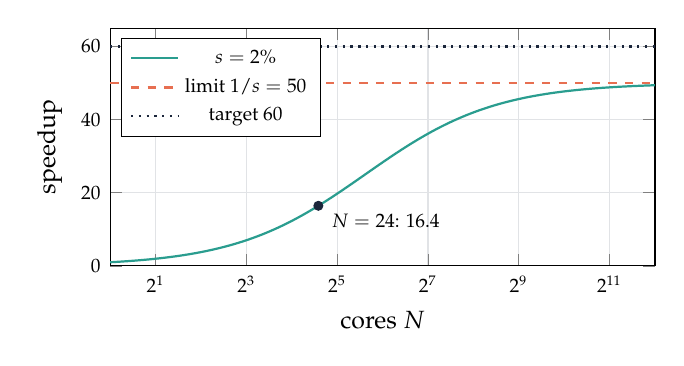
\begin{tikzpicture}
\begin{axis}[width=8.5cm,height=4.6cm,xmode=log,log basis x=2,xlabel={cores $N$},ylabel={speedup},
  xmin=1,xmax=4096,ymin=0,ymax=65,grid=both,grid style={draw=slate!20},tick label style={font=\scriptsize},
  label style={font=\small},legend style={font=\scriptsize,at={(0.02,0.96)},anchor=north west}]
\addplot[thick,teal,domain=1:4096,samples=120]{1/(0.02+0.98/x)};
\addplot[thick,dashed,coral,domain=1:4096]{50};
\addplot[thick,dotted,ink,domain=1:4096]{60};
\addplot[only marks,mark=*,mark size=1.6pt,ink] coordinates {(24,16.44)};
\node[tk,anchor=north west] at (axis cs:28,15){$N=24$: 16.4};
\legend{$s=2\%$,limit $1/s=50$,target 60}
\end{axis}\end{tikzpicture}}
To reach $60\times$ the serial part itself must change:
\begin{itemize}
  \item \textbf{Shrink the serial fraction} below $1/60=1.67\%$ (better algorithm, parallelise more of the code).
        For example, with $s=1\%$: $0.01+0.99/N=1/60\Rightarrow N\approx149$ cores.
  \item \textbf{Speed up the serial part} with faster single-thread hardware (a higher clock or better
        microarchitecture). This breaks the ``same speed on all cores'' assumption.
  \item Add far more cores, beyond 24 (needed in either case).
\end{itemize}
\ans{\textbf{No.} With 2\% serial code the speedup can never exceed $1/0.02=50\times$ (Amdahl's law). $60\times$ needs
the serial fraction reduced below $1.67\%$, plus well over 24 cores.}
\end{solution}

%---------------------------------------------------------------- PF06
\begin{question}{2021--2022 \textbullet\ Q8(a)}{CSE 305 \textbullet\ 06/04/2023 \textbullet\ PF06}{3 + 3 + 5}
Consider two different implementations (P1 and P2) of the same instruction set architecture. There are three
classes of instructions A, B, and C. Suppose, a program has 200,000 instructions divided into three classes as
25\% class A, 60\% class B, and 15\% class C. The clock rate and CPI of each implementation are given in the
following table (Table: 8.a).
\fig{\begin{tabular}{|c|c|c|c|c|}\hline
Implementation & Clock Rate & CPI of Class A & CPI of Class B & CPI of Class C\\\hline
P1 & 2.7\,GHz & 3 & 3 & 2\\\hline
P2 & 3.5\,GHz & 2 & 4 & 1\\\hline
\end{tabular}}
\begin{center}\small Table: 8.a\end{center}
\begin{enumerate}
  \item Find the total clock cycle required in both implementations.
  \item Calculate the execution time required for both implementations and determine which implementation is
        faster.
  \item How much must we improve the CPI of Class C instructions if we want the program to run two times faster
        in the better implementation determined in the previous question?
\end{enumerate}
\end{question}
\begin{solution}
\textbf{Method.} Cycles $=\sum_i \text{IC}_i\,\text{CPI}_i$, \ $T=\text{Cycles}/\text{Clock rate}$. For a target time,
solve $\text{Cycles}_{\text{target}}=\text{Cycles}_{\text{other classes}}+\text{IC}_C\cdot\text{CPI}_C^{\text{new}}$.

Counts: A $=50{,}000$, B $=120{,}000$, C $=30{,}000$.

\textbf{(i)} $\text{Cycles}_{P1}=50\text{k}(3)+120\text{k}(3)+30\text{k}(2)=150\text{k}+360\text{k}+60\text{k}=570{,}000$.\\
\phantom{\textbf{(i)} }$\text{Cycles}_{P2}=50\text{k}(2)+120\text{k}(4)+30\text{k}(1)=100\text{k}+480\text{k}+30\text{k}=610{,}000$.

\textbf{(ii)} $T_{P1}=570{,}000/2.7\times10^{9}=211.1\,\mu$s;\quad $T_{P2}=610{,}000/3.5\times10^{9}=174.3\,\mu$s.
So P2 is faster, by $211.1/174.3=1.21\times$.

\textbf{(iii)} In P2, twice as fast needs $T=87.14\,\mu$s, i.e.\ $305{,}000$ cycles. The class A and B cycles alone are
$100\text{k}+480\text{k}=580{,}000>305{,}000$:
\[
580{,}000+30{,}000\cdot\text{CPI}_C^{\text{new}}=305{,}000\ \Rightarrow\ \text{CPI}_C^{\text{new}}=-9.17\quad(\text{impossible}).
\]
Even with $\text{CPI}_C=0$, the speedup is only $610/580=1.05\times$ (Amdahl's law).
\ans{(i) 570{,}000 and 610{,}000 cycles. (ii) $211.1\,\mu$s vs.\ $174.3\,\mu$s, so \textbf{P2} is faster ($1.21\times$).
(iii) \textbf{Not possible.} Class C contributes only $30{,}000$ of P2's $610{,}000$ cycles.}
\end{solution}

%---------------------------------------------------------------- PF07
\repeated{4}
\begin{question}{2020--2021 \textbullet\ Q1}{CSE 305 \textbullet\ 24/09/2022 \textbullet\ PF07}{15}
You have surely learnt about the eight big ideas of computer architecture. They are again mentioned below to
brush up your memory:
\begin{itemize}[itemsep=0pt]
  \item Design for Moore's Law
  \item Use abstraction to simplify design
  \item Make the common case fast
  \item Performance via parallelism
  \item Performance via pipelining
  \item Performance via prediction
  \item Hierarchy of memories
  \item Dependability via redundancy
\end{itemize}
Now identify the statements below best relate to which of the above ideas. Each statement should relate to a
single idea. Elaborate the justification behind your answer.
\begin{itemize}[label={}]
  \item \textit{(a) Code reordering is done to avoid the use of load result in the next instruction.}
  \item \textit{(b) Different caches for data and memory can effectively increase bandwidth.}
  \item \textit{(c) As CPUs have hit their physical performance barrier due to power limit issues, GPUs have
        started gaining increased popularity among the programming community.}
\end{itemize}
\end{question}
\begin{question}{2020--2021 \textbullet\ Q10(a)}{CSE 305 \textbullet\ 24/09/2022 \textbullet\ PF07}{12}
Briefly explain the eight great ideas in Computer Architecture.
\end{question}
\begin{question}{2016--2017 \textbullet\ Q5(a)}{CSE 305 \textbullet\ 02/08/2017 \textbullet\ PF07}{10}
``Computer architectures have invented several great ideas in the last 60 years of computer design. These ideas
are so powerful that they have lasted long after the first computer that used them, with newer architects
demonstrating their admiration by imitating their predecessors.'' These ideas include:
(i) Design for Moore's Law \quad (ii) Use abstraction to simplify design \quad (iii) Make the common case faster
\quad (iv) Performance via parallelism \quad (v) Performance via pipelining \quad (vi) Performance via prediction
\quad (vii) Hierarchy of memories \quad (viii) Dependability via redundancy.

You are given several design features of MIPS and other modern computing systems in the following. Now, please
\textbf{identify} that which of the above great ideas are behind these design decisions.
\begin{enumerate}
  \item While implementing instructions at hardware level, it is possible to implement all the instructions as
        single cycle instructions. However, modern designers do not use this single-cycle design as it is
        inefficient. (hint: for single cycle implementation, the clock cycle must have the same length for every
        instruction and the longest instruction determine the clock cycle length.)
  \item Modern computers use a technique called prefetching. ``In prefetching, a block of data is brought into
        the cache before it is actually referenced. Many microprocessors use hardware perfectching to access the
        block needed in the future that may be difficult for software to notice''.
\end{enumerate}
\end{question}
\begin{question}{2014--2015 \textbullet\ Q5(a)}{CSE 305 \textbullet\ 26/01/2016 \textbullet\ PF07}{20}
``Computer architects have invented several great ideas in the last 60 years of computer design. These ideas
are so powerful that they have lasted long after the first computer that used them, with newer architects
demonstrating their admiration by imitating their predecessors''. These ideas include:
1.~Design for Moore's Law \quad 2.~Use abstraction to simplify design \quad 3.~Make the common case faster \quad
4.~Performance via parallelism \quad 5.~Performance via pipelining \quad 6.~Performance via prediction \quad
7.~Hierarchy of memories \quad 8.~Dependability via redundancy.

You are given several design features of MIPS and other modern computing systems in the following. Now, please
\textbf{identify} that which of the above great ideas are behind these design decisions.
\begin{enumerate}[label=\textbf{\arabic*.}]
  \item In MIPS datapath, there is an adder which computes the value of \textbf{(PC+4)}, where PC means Program
        Counter. For branch addressing the MIPS address is actually relative to this \textbf{(PC+4)} rather than
        \textbf{(PC)}. This form of branch addressing is called PC-relative addressing.
  \item In the past, most PCs (personal computers) and server systems used separate SRAM (static random access
        memory) chips for either their primary, secondary, or even tertiary caches. Today, all levels of caches
        are integrated onto the processor chip, so the market for separate SRAM chips has nearly evaporated.
  \item A fast multiplication hardware, ``unrolls the loop'' by using 31 adders rather than using a single 32-bit
        adder 31 times.
  \item Procedures or Functions allow programmers to concentrate on just one portion of the task at a time,
        parameters act as an interface between the procedure and the rest of the program and data, since they can
        pass values and return results.
  \item Modern computers use a technique called prefetching. In prefetching, a block of data is brought into the
        cache before it is actually referenced. Many microprocessors use hardware prefetching to access the block
        needed in the future that may be difficult for software to notice.
\end{enumerate}
\end{question}
\begin{solution}
\sub{The eight great ideas (answer to 2020--2021 Q10(a); used by every card)}
{\small\renewcommand{\arraystretch}{1.15}
\begin{tabularx}{\linewidth}{@{}>{\raggedright\arraybackslash\bfseries}p{3.9cm}X@{}}
\toprule
Idea & What it means \\\midrule
Design for Moore's Law & Transistor counts double every 18--24 months. A design takes years, so architects
target the technology that will exist when it ships, not when it starts.\\
Use abstraction to simplify design & Hide lower-level detail behind clean interfaces (ISA, ABI, procedures,
OS) so that each level can be designed and understood separately. This raises productivity.\\
Make the common case fast & Optimise what happens most often; this pays off more than optimising rare cases
(Amdahl's law).\\
Performance via parallelism & Do several operations at the same time: multiple ALUs or adders, multicore,
SIMD, multiple issue.\\
Performance via pipelining & A special form of parallelism. Overlap the stages of successive operations like
an assembly line, so throughput rises.\\
Performance via prediction & It can be faster on average to guess and start working than to wait, provided
recovery from a wrong guess is cheap and guesses are usually right (branch prediction, prefetching).\\
Hierarchy of memories & Fastest, smallest, costliest memory at the top (caches), slower, larger, cheaper memory
below (DRAM, disk). This gives the illusion of memory that is both fast and large.\\
Dependability via redundancy & Include spare or duplicate components so the system keeps working when one fails
(RAID, ECC, duplicated servers).\\
\bottomrule
\end{tabularx}}

\sub{2020--2021 Q1}
\begin{itemize}
  \item[(a)] \key{Performance via pipelining.} In a pipeline, a loaded value is available only after MEM, so an
        instruction that uses it immediately causes a load-use hazard and a stall. Reordering independent
        instructions into the slot after the load keeps the pipeline full (no bubble). This problem exists only
        because the instructions are pipelined.
  \item[(b)] \key{Hierarchy of memories.} Splitting the first cache level into an I-cache and a D-cache refines
        the top of the memory hierarchy: an instruction fetch and a data access can be served by the fast
        small memories in the same cycle, which doubles the bandwidth seen by the processor. (The statement
        means separate caches for data and \emph{instructions}.)
  \item[(c)] \key{Performance via parallelism.} The power wall stopped clock-rate growth, so single-core
        performance stalled. GPUs gain performance by running thousands of simple threads in parallel, which is
        why programmers moved to them.
\end{itemize}

\sub{2016--2017 Q5(a)}
\begin{enumerate}
  \item \key{Performance via pipelining}, motivated by \emph{make the common case fast}. In a single-cycle
        design the slowest instruction (\ins{lw}) sets the clock period for every instruction, so common fast
        instructions are slowed down. Splitting execution into short equal stages and overlapping them
        (pipelining) gives a short clock and a CPI near 1.
  \item \key{Performance via prediction}, within the hierarchy of memories. The hardware guesses which block
        will be needed next and brings it into the cache early. A correct guess turns a miss into a hit; a wrong
        guess costs only some bandwidth.
\end{enumerate}

\sub{2014--2015 Q5(a)}
\begin{enumerate}[label=\textbf{\arabic*.}]
  \item \key{Make the common case fast.} PC$+4$ has already been computed for the sequential (most common)
        path, and most branch targets are near the branch. Making the offset relative to PC$+4$ reuses that
        adder output and reaches nearby targets with a 16-bit offset.
  \item \key{Design for Moore's Law.} The growing number of transistors per chip let whole cache levels move on
        die. Designers planned for this transistor budget, and separate SRAM chips disappeared.
  \item \key{Performance via parallelism.} 31 adders work simultaneously (a tree of adders) instead of one adder
        being reused sequentially 31 times.
  \item \key{Use abstraction to simplify design.} A procedure hides its implementation behind an interface
        (parameters and return value), so the programmer deals with one piece at a time.
  \item \key{Performance via prediction.} The hardware predicts future accesses and fetches blocks before they
        are referenced. (The prefetched block then sits in the cache, part of the memory hierarchy.)
\end{enumerate}
\ans{Q1: (a) pipelining, (b) hierarchy of memories, (c) parallelism. 2016--17: (i) pipelining (make the common case fast),
(ii) prediction. 2014--15: 1 common case fast, 2 Moore's Law, 3 parallelism, 4 abstraction, 5 prediction.}
\end{solution}

%---------------------------------------------------------------- PF08
\begin{question}{2020--2021 \textbullet\ Q2}{CSE 305 \textbullet\ 24/09/2022 \textbullet\ PF08}{15}
What is your most favorite topic learnt from processor, memory hierarchy, and multiprocessors? Describe briefly.
\end{question}
\begin{solution}
\begin{note}This is an open question; any well-explained topic earns credit. Below is a model answer on
\textbf{pipelining} (from the processor part). A good answer names the topic, explains the core idea, gives a
small example or diagram, and mentions its issues or limits.\end{note}

\sub{Favourite topic: pipelining in the MIPS processor}
\textbf{Idea.} Instruction execution is split into five stages, each taking one clock cycle:
IF (fetch), ID (decode / register read), EX (ALU), MEM (data memory), WB (register write-back).
Pipeline registers (IF/ID, ID/EX, EX/MEM, MEM/WB) separate the stages, so a new instruction can enter every
cycle, like an assembly line.
\fig{{\small\setlength{\tabcolsep}{1pt}\begin{tabular}{l*{7}{P}}
 & 1&2&3&4&5&6&7\\
\ins{lw \ \$t0,0(\$s0)} &\IF&\ID&\EX&\MEM&\WB&&\\
\ins{add \$t1,\$t2,\$t3} & &\IF&\ID&\EX&\MEM&\WB&\\
\ins{sub \$t4,\$t5,\$t6} & & &\IF&\ID&\EX&\MEM&\WB\\
\end{tabular}}}
\textbf{Why I like it.}
\begin{itemize}
  \item Throughput rises without making any single instruction faster. Ideal speedup $\approx$ number of stages.
        With stage times 200/100/200/200/100\,ps, a single-cycle CPU needs 800\,ps per instruction; the pipeline
        completes one every 200\,ps, i.e.\ $4\times$ for long programs.
  \item It shows a whole chain of design trade-offs, the \key{hazards}:
    \begin{itemize}
      \item \emph{Structural}: two stages need the same hardware. MIPS avoids this with separate I- and D-memory.
      \item \emph{Data}: an instruction needs a result that is not yet written back. Fixes: \key{forwarding}
            (EX/MEM, MEM/WB $\rightarrow$ ALU inputs), a hazard-detection unit that stalls one cycle for a load-use
            hazard, and compiler code scheduling.
      \item \emph{Control}: the branch outcome is not known in time. Fixes: move the branch comparison into ID,
            predict (static, or dynamic with 1-/2-bit predictors), or use delayed branches.
    \end{itemize}
  \item It extends naturally to deeper pipelines and to multiple issue (superscalar/VLIW), which is the
        instruction-level parallelism used by modern CPUs.
\end{itemize}
\textbf{Takeaway:} $\text{Time}=\text{IC}\times\text{CPI}\times T_c$. Pipelining cuts $T_c$ while keeping CPI close to 1;
hazards are what push CPI above 1.
\end{solution}

%---------------------------------------------------------------- PF09
\begin{question}{2020--2021 \textbullet\ Q12(a)}{CSE 305 \textbullet\ 24/09/2022 \textbullet\ PF09}{8}
The data for the two programs A and B are given below.
\fig{\begin{tabular}{|l|>{\centering\arraybackslash}p{3cm}|>{\centering\arraybackslash}p{2.6cm}|>{\centering\arraybackslash}p{2.6cm}|}\hline
\textbf{Instruction Type} & \textbf{Clock Cycle per Instruction (CPI)} & \textbf{Instruction Count in Program A} & \textbf{Instruction Count in Program B}\\\hline
Multiplication & 3 & 2 & 3\\\hline
Addition & 1 & 1 & 2\\\hline
Subtraction & 2 & 4 & 3\\\hline
Division & 4 & 2 & 2\\\hline
\end{tabular}}
Which program has the higher average clock cycle per instruction?
\end{question}
\begin{solution}
Average CPI $=\dfrac{\sum_i \text{IC}_i\times\text{CPI}_i}{\sum_i\text{IC}_i}$.
\fig{\begin{tabular}{lccccc}\toprule
 & CPI & IC$_A$ & cycles$_A$ & IC$_B$ & cycles$_B$\\\midrule
Multiplication & 3 & 2 & 6 & 3 & 9\\
Addition & 1 & 1 & 1 & 2 & 2\\
Subtraction & 2 & 4 & 8 & 3 & 6\\
Division & 4 & 2 & 8 & 2 & 8\\\midrule
Total & & 9 & 23 & 10 & 25\\\bottomrule
\end{tabular}}
\[
\overline{\text{CPI}}_A=\frac{23}{9}=2.56,\qquad \overline{\text{CPI}}_B=\frac{25}{10}=2.50 .
\]
\ans{\textbf{Program A} has the higher average CPI (2.56 vs.\ 2.50). Program B still takes more total cycles
(25 vs.\ 23) because it executes more instructions.}
\end{solution}

%---------------------------------------------------------------- PF10
\begin{question}{2019--2020 \textbullet\ Q1(a)}{CSE 305 \textbullet\ 18/09/2021 \textbullet\ PF10}{15}
Suppose we want to compare the performance of \emph{Computer System A} with \emph{Computer System B}. For this
purpose, \emph{Program 1} is run in both the computer systems and corresponding information (logs) are captured.
The logs are presented below in Table 1.1 and Table 1.2.
\fig{{\footnotesize\renewcommand{\arraystretch}{1.1}\begin{tabular}{@{}c@{\quad}c@{}}
\begin{tabular}{|l|>{\centering\arraybackslash}p{1.9cm}|}\hline
\textbf{Operation} & \textbf{Required Clock Cycle(s)}\\\hline
Multiplication 1 of Program 1 & 4\\\hline
Addition 1 of Program 2 & 2\\\hline
I/O overhead time required by OS & 5\\\hline
Multiplication 2 of Program 1 & 4\\\hline
Division 1 of Program 1 & 5\\\hline
Multiplication 1 of Program 2 & 4\\\hline
I/O overhead time required by OS & 2\\\hline
Division 2 of Program 1 & 5\\\hline
I/O overhead time required by OS & 4\\\hline
Addition 1 of Program 3 & 2\\\hline
Addition 1 of Program 1 & 2\\\hline
\multicolumn{2}{c}{\textbf{Table 1.1: Logs from Computer System A}}
\end{tabular}
&
\begin{tabular}{|l|>{\centering\arraybackslash}p{1.9cm}|}\hline
\textbf{Operation} & \textbf{Required Clock Cycle(s)}\\\hline
Multiplication 1 of Program 4 & 5\\\hline
Multiplication 1 of Program 1 & 5\\\hline
I/O overhead time required by OS & 1\\\hline
Multiplication 2 of Program 1 & 5\\\hline
Division 1 of Program 1 & 6\\\hline
Multiplication 2 of Program 4 & 5\\\hline
Addition 1 of Program 4 & 3\\\hline
I/O overhead time required by OS & 3\\\hline
Addition 2 of Program 4 & 3\\\hline
Division 2 of Program 1 & 6\\\hline
Addition 1 of Program 1 & 3\\\hline
\multicolumn{2}{c}{\textbf{Table 1.2: Logs from Computer System B}}
\end{tabular}
\end{tabular}}}
If the clock rates of \emph{Computer System A} and \emph{Computer System B} are 2\,GHz and 2.5\,GHz respectively,
then compare their performances based on the execution time of \emph{Program 1}.
\end{question}
\begin{solution}
\textbf{Key idea.} The performance of a program is judged by its own \key{CPU time}. CPU time counts only the
cycles spent executing that program's work; it \emph{discounts} OS I/O overhead and other jobs' shares (slide:
Measuring Execution Time). So keep only the ``of Program 1'' rows.

\fig{\begin{tabular}{lcc}\toprule
Program 1 operation & System A cycles & System B cycles\\\midrule
Multiplication 1 & 4 & 5\\
Multiplication 2 & 4 & 5\\
Division 1 & 5 & 6\\
Division 2 & 5 & 6\\
Addition 1 & 2 & 3\\\midrule
\textbf{Total} & \textbf{20} & \textbf{25}\\\bottomrule
\end{tabular}}
\[
T_A=\frac{20}{2\times10^{9}}=10\text{ ns},\qquad
T_B=\frac{25}{2.5\times10^{9}}=10\text{ ns},\qquad
\frac{\text{Perf}_A}{\text{Perf}_B}=\frac{T_B}{T_A}=1 .
\]
\ans{CPU time of Program 1 is \textbf{10\,ns on both} systems, so A and B have \textbf{equal performance} for Program 1.
B's higher clock rate (2.5 vs.\ 2\,GHz) is exactly cancelled by its 25\% more cycles.}
\begin{note}If one wrongly adds the OS I/O rows (A: $5+2+4=11$, B: $1+3=4$ cycles), the totals become A $=31$ cycles
$=15.5$\,ns and B $=29$ cycles $=11.6$\,ns. That measures system/elapsed behaviour, not Program 1's CPU time.
Rows of Programs 2, 3 and 4 belong to other jobs and are always excluded.\end{note}
\end{solution}

%---------------------------------------------------------------- PF11
\begin{question}{2019--2020 \textbullet\ Q1(b)}{CSE 305 \textbullet\ 18/09/2021 \textbullet\ PF11}{4 + 8}
What is the importance of Moore's Law? ``To increase the overall performance of a computer by $x$ amount, it is
required to identify the most important aspect of the computer and improve its performance by $x$ amount.'' Do you
agree or disagree with the statement? Justify your answer with proper mathematical explanation.
\end{question}
\begin{solution}
\sub{Importance of Moore's Law}
\begin{itemize}
  \item Transistors per chip double about every 18--24 months. This exponential growth has driven the steady
        gains in cost and performance, and made new applications possible (mobile devices, the web, genome work).
  \item It is a \key{design target}: a processor takes years to design, so architects must plan for the
        transistor budget available when the product ships (``Design for Moore's Law'').
  \item It turns extra transistors into features: on-chip caches, multiple cores, wider issue.
\end{itemize}

\sub{The statement: disagree (Amdahl's law)}
Improving one aspect by a factor $x$ speeds up only the part of the time that aspect uses:
\[
T_{\text{improved}}=\frac{T_{\text{affected}}}{x}+T_{\text{unaffected}},\qquad
\text{Speedup}=\frac{1}{(1-F)+F/x}
\]
where $F$ is the fraction of time affected. Overall speedup $=x$ only if $F=1$. For any $F<1$ the speedup is
$<x$, and it can never exceed $1/(1-F)$, however large $x$ is.

\textbf{Example (slides).} Multiply takes 80\,s of a 100\,s program. To get $5\times$ overall we need 20\,s:
\[
20=\frac{80}{n}+20\ \Rightarrow\ \frac{80}{n}=0\quad\text{(impossible).}
\]
Even improving multiply by $5\times$ gives only $100/(16+20)=2.78\times$, not $5\times$.
\ans{\textbf{Disagree.} Improving one aspect by $x$ gives overall speedup $1/((1-F)+F/x)<x$ unless that aspect is 100\% of
the time. The right strategy is \emph{make the common case fast} and improve every significant part, not one part alone.}
\end{solution}

%---------------------------------------------------------------- PF12
\begin{question}{2018--2019 \textbullet\ Q7(b)}{CSE 305 \textbullet\ 29/10/2019 \textbullet\ PF12}{20}
Assume that a processor with 4\,GHz clock rate is executing a program that requires the following instruction types.
\fig{\begin{tabular}{|l|c|c|c|c|}\hline
\textbf{Instructions} & \textbf{FP} & \textbf{INT} & \textbf{L/S} & \textbf{BRANCH}\\\hline
Instruction Count ($\times10^6$) & 160 & 110 & 10 & 16\\\hline
CPI & 2 & 1 & 5 & 2\\\hline
\end{tabular}}
\begin{enumerate}
  \item Calculate the execution time of the program.
  \item If you want the program to run two times faster, then how much should you improve the CPI of
        \textbf{FP} instructions? Explain your finding.
  \item If you want the program to run two times faster, then how much should you improve the CPI of
        \textbf{L/S} instructions? Explain your finding.
  \item By how much is the execution time changed if the \textbf{CPI} of \textbf{INT} and \textbf{BRANCH}
        instructions are increased by 15\% and the \textbf{CPI} of \textbf{FP} and \textbf{L/S} instructions are
        decreased by 20\%?
\end{enumerate}
\end{question}
\begin{solution}
\textbf{Method.} $\text{Cycles}=\sum \text{IC}_i\cdot\text{CPI}_i$, \ $T=\text{Cycles}/f$. ``Two times faster'' at the same
clock means half the cycles. A class can deliver this only if
$\text{Cycles}_{\text{others}}+\text{IC}_k\cdot\text{CPI}_k^{\text{new}}=\tfrac12\text{Cycles}$ has a solution with
$\text{CPI}_k^{\text{new}}>0$.
\fig{\begin{tabular}{lcccc|c}\toprule
 & FP & INT & L/S & BR & Total\\\midrule
cycles ($10^6$) & $160\times2=320$ & $110\times1=110$ & $10\times5=50$ & $16\times2=32$ & \textbf{512}\\\bottomrule
\end{tabular}}
\textbf{(i)} $T=512\times10^{6}/4\times10^{9}=0.128$\,s.

\textbf{(ii)} Target $=256$\,M cycles. Non-FP cycles $=110+50+32=192$\,M, so
\[
192+160\cdot\text{CPI}_{FP}^{\text{new}}=256\ \Rightarrow\ \text{CPI}_{FP}^{\text{new}}=\frac{64}{160}=0.4 .
\]
FP is the dominant class (62.5\% of the cycles), so improving it can reach the target: its CPI must drop from 2 to
0.4, a \key{$5\times$ improvement} (80\% reduction).

\textbf{(iii)} Non-L/S cycles $=320+110+32=462$\,M $>256$\,M:
\[
462+10\cdot\text{CPI}_{L/S}^{\text{new}}=256\ \Rightarrow\ \text{CPI}_{L/S}^{\text{new}}=-20.6\quad\text{(impossible).}
\]
L/S is only $50/512\approx9.8\%$ of the cycles. Even $\text{CPI}_{L/S}=0$ gives at most $512/462=1.11\times$ (Amdahl's law).

\textbf{(iv)} New CPIs: INT $1.15$, BR $2.30$, FP $1.6$, L/S $4.0$.
\[
\text{Cycles}'=160(1.6)+110(1.15)+10(4)+16(2.3)=256+126.5+40+36.8=459.3\text{ M}
\]
$T'=459.3\times10^6/4\times10^9=0.1148$\,s. Change $=(512-459.3)/512=10.3\%$ less time (speedup $1.115\times$).
\ans{(i) 0.128\,s. (ii) CPI$_{FP}$: $2\rightarrow0.4$ ($5\times$ better). (iii) \textbf{Impossible} through L/S alone.
(iv) Execution time falls by $\approx$10.3\% (0.128\,s $\rightarrow$ 0.1148\,s).}
\end{solution}

%---------------------------------------------------------------- PF13
\begin{question}{2017--2018 \textbullet\ Q5(a)}{CSE 305 \textbullet\ 23/09/2018 \textbullet\ PF13}{8 + 7}
Suppose there are three classes of instructions A, B and C in a particular instruction set architecture with
CPIs 1.2, 2 and 2.5, respectively. The number of instructions from each class in two separate programs P1 and
P2 are as follows:
\fig{\begin{tabular}{|c|c|c|c|}\hline
\multirow{2}{*}{Programs} & \multicolumn{3}{c|}{Instruction Classes}\\\cline{2-4}
 & A & B & C\\\hline
P1 & 40 & 10 & 16\\\hline
P2 & 12 & 13 & 40\\\hline
\end{tabular}}
\begin{enumerate}
  \item Which program will execute faster and by how much?
  \item By how much should we improve the CPI of Instruction Class B to make P1 execute two times faster?
        Explain your finding.
\end{enumerate}
\end{question}
\begin{solution}
\textbf{Method.} Cycles $=\sum_i \text{IC}_i\,\text{CPI}_i$. Both programs run on the same machine (same clock), so
execution time $\propto$ cycles.

\textbf{(i)} $\text{Cycles}_{P1}=40(1.2)+10(2)+16(2.5)=48+20+40=108$;\quad
$\text{Cycles}_{P2}=12(1.2)+13(2)+40(2.5)=14.4+26+100=140.4$.\\
$140.4/108=1.3$.

\textbf{(ii)} For P1 to run twice as fast it needs $108/2=54$ cycles. Classes A and C alone need $48+40=88>54$:
\[
88+10\cdot\text{CPI}_B^{\text{new}}=54\ \Rightarrow\ \text{CPI}_B^{\text{new}}=-3.4\quad(\text{impossible}).
\]
Class B accounts for only $20/108=18.5\%$ of P1's time. By Amdahl's law the best possible gain is
$108/88=1.23\times$ (with $\text{CPI}_B=0$).
\ans{(i) \textbf{P1} is faster, by $\mathbf{1.3\times}$ (108 vs.\ 140.4 cycles). (ii) \textbf{Impossible}: no CPI$_B$ improvement can
give $2\times$; the maximum is $1.23\times$.}
\end{solution}

%---------------------------------------------------------------- PF14
\begin{question}{2016--2017 \textbullet\ Q5(c)}{CSE 305 \textbullet\ 02/08/2017 \textbullet\ PF14}{15}
Assume a processor with 3\,GHz clock rate is executing a program that requires following instructions,
\fig{\begin{tabular}{|l|c|c|c|c|}\hline
Instructions $\rightarrow$ & \textbf{FP} & \textbf{INT} & \textbf{L/S} & \textbf{BRANCH}\\\hline
Instruction Count ($\times10^6$) & 40 & 80 & 90 & 15\\\hline
\textbf{CPI} & 1 & 1 & 3 & 2\\\hline
\end{tabular}}
\begin{enumerate}
  \item Calculate the execution time of the program.
  \item By how much must we improve the CPI of \textbf{FP} instructions if we want the program to run two times
        faster?
  \item By how much is the execution time program changed (improved or degraded) if the \textbf{CPI} of
        \textbf{INT} and \textbf{FP} instruction is increased by 20\% and the \textbf{CPI} of \textbf{L/S} and
        Branch is reduced by 10\%?
\end{enumerate}
\end{question}
\begin{solution}
\textbf{Method.} $\text{Cycles}=\sum \text{IC}_i\cdot\text{CPI}_i$, \ $T=\text{Cycles}/f$. ``Two times faster'' at the same
clock means half the cycles, which must be reachable with $\text{CPI}_{FP}^{\text{new}}>0$.

\textbf{(i)} $\text{Cycles}=40(1)+80(1)+90(3)+15(2)=40+80+270+30=420$\,M, so $T=420\times10^6/3\times10^9=0.14$\,s.

\textbf{(ii)} Target 210\,M cycles. Non-FP cycles $=80+270+30=380$\,M $>210$\,M, so
$\text{CPI}_{FP}^{\text{new}}=(210-380)/40<0$, which is \key{impossible}. FP is only $40/420=9.5\%$ of the cycles; the
best possible is $420/380=1.105\times$. (The heavy class here is L/S, 64\% of the cycles.)

\textbf{(iii)} New CPIs: FP $1.2$, INT $1.2$, L/S $2.7$, BR $1.8$.
\[
\text{Cycles}'=40(1.2)+80(1.2)+90(2.7)+15(1.8)=48+96+243+27=414\text{ M},\qquad T'=0.138\text{ s}.
\]
\ans{(i) 0.14\,s. (ii) \textbf{Not possible} by improving FP alone. (iii) \textbf{Improved} slightly: $0.14\rightarrow0.138$\,s,
i.e.\ 1.43\% less time (speedup $1.014\times$). The 10\% L/S saving outweighs the 20\% FP/INT penalty.}
\end{solution}

%---------------------------------------------------------------- PF15
\begin{question}{2015--2016 \textbullet\ Q1(a)}{CSE 305 \textbullet\ 18/01/2017 \textbullet\ PF15}{10}
Consider three different processors P1, P2 and P3 executing the same instruction set. P1 has a 3\,GHz clock rate
and a CPI of 1.5. P2 has a 2.5\,GHz clock rate and a CPI of 1.0. P3 has a 4.0\,GHz clock rate and has a CPI of 2.2.
\begin{enumerate}
  \item Which processor has the highest performance expressed in instructions per second?
  \item If the processors each execute a program in 10 seconds, find the number of cycles and the number of
        instructions.
  \item We are trying to reduce the execution time by 30\% but this leads to an increase of 20\% in the CPI. What
        clock rate should we have to get this time reduction?
\end{enumerate}
\end{question}
\begin{solution}
\sub{(i) Instructions per second $=$ clock rate / CPI}
P1: $3\times10^9/1.5=2.0\times10^9$;\quad P2: $2.5\times10^9/1.0=2.5\times10^9$;\quad P3: $4\times10^9/2.2=1.82\times10^9$.
\ans{\textbf{P2} has the highest performance: $2.5\times10^9$ instructions/s.}

\sub{(ii) Program runs 10\,s: cycles $=T\times f$, instructions $=$ cycles / CPI}
\fig{\begin{tabular}{lccc}\toprule
 & P1 & P2 & P3\\\midrule
Cycles & $3\times10^{10}$ & $2.5\times10^{10}$ & $4\times10^{10}$\\
Instructions & $2\times10^{10}$ & $2.5\times10^{10}$ & $1.82\times10^{10}$\\\bottomrule
\end{tabular}}

\sub{(iii) New time $0.7T$, new CPI $1.2\,\text{CPI}$, same IC}
\[
0.7\,\frac{\text{IC}\cdot\text{CPI}}{f}=\frac{\text{IC}\cdot1.2\,\text{CPI}}{f_{\text{new}}}
\ \Rightarrow\ f_{\text{new}}=\frac{1.2}{0.7}f=1.714\,f .
\]
\ans{Required clock rates: P1 $3\rightarrow\mathbf{5.14}$\,GHz, P2 $2.5\rightarrow\mathbf{4.29}$\,GHz, P3 $4\rightarrow\mathbf{6.86}$\,GHz
(each $1.714\times$ the old rate).}
\end{solution}

%---------------------------------------------------------------- PF16
\begin{question}{2015--2016 \textbullet\ Q1(b)}{CSE 305 \textbullet\ 18/01/2017 \textbullet\ PF16}{10}
The following table shows the numbers of instructions for a program.
\fig{\begin{tabular}{|c|c|c|c|}\hline
Arithmetic & Store & Load & Branch\\\hline
500 & 50 & 100 & 50\\\hline
\end{tabular}}
The following table shows the number of cycles taken by each instruction.
\fig{\begin{tabular}{|c|c|c|c|}\hline
Arithmetic & Store & Load & Branch\\\hline
1 & 5 & 5 & 2\\\hline
\end{tabular}}
\begin{enumerate}
  \item What is the execution time of the program in a 4\,GHz processor?
  \item What is the CPI of the program?
  \item If the number of load instructions can be reduced by half, what is the speed-up and CPI?
\end{enumerate}
\end{question}
\begin{solution}
\fig{\begin{tabular}{lcccc|c}\toprule
 & Arithmetic & Store & Load & Branch & Total\\\midrule
IC & 500 & 50 & 100 & 50 & 700\\
Cycles & 500 & 250 & 500 & 100 & 1350\\\midrule
IC (loads halved) & 500 & 50 & 50 & 50 & 650\\
Cycles (loads halved) & 500 & 250 & 250 & 100 & 1100\\\bottomrule
\end{tabular}}
(i) $T=\dfrac{1350}{4\times10^{9}}=337.5$\,ns.

(ii) $\text{CPI}=\dfrac{1350}{700}=1.93$.

(iii) $T'=1100/4\times10^9=275$\,ns, so
$\text{Speedup}=\dfrac{1350}{1100}=1.23$ and $\text{CPI}'=\dfrac{1100}{650}=1.69$.
\ans{(i) 337.5\,ns. (ii) CPI $=1.93$. (iii) Speedup $=\mathbf{1.23\times}$ and new CPI $=\mathbf{1.69}$. Removing
slow 5-cycle loads lowers both the cycle count and the average CPI.}
\end{solution}

%---------------------------------------------------------------- PF17
\begin{question}{2015--2016 \textbullet\ Q1(c)}{CSE 305 \textbullet\ 18/01/2017 \textbullet\ PF17}{15}
Assume for arithmetic, load/store, and branch instructions, a processor has CPIs of 1, 12, and 5, respectively.
Also, assume that on a single processor a program requires the execution of 2.56 billion arithmetic
instructions, 1.28 billion load/store instructions, and 256 million branch instructions. Assume that each
processor has a 2\,GHz clock frequency. Assume that, as the program is parallelized to run over multiple cores,
the number of arithmetic and load/store instructions per processor is divided by $0.7\times p$ (where $p$ is the
number of processors) but the number of branch instructions per processor remains the same.
(1 billion $=10^9$, 1 million $=10^6$).
\begin{enumerate}
  \item Find the total execution time for this program on 1, 2, and 4 processors, and show the relative speedup
        of the 2, and 4 processors compared to the single processor.
  \item If the CPI of the arithmetic instructions was doubled, what would the impact be on the execution time of
        the program on 1, 2, and 4 processors?
  \item How much should the CPI of load/store instructions be reduced for a single processor to match the
        performance of 4 processors using the original CPI values?
\end{enumerate}
\end{question}
\begin{solution}
\textbf{Model.} Cycles per processor:
\[
C(p)=\frac{\text{IC}_{ar}\text{CPI}_{ar}+\text{IC}_{ls}\text{CPI}_{ls}}{0.7\,p}+\text{IC}_{br}\text{CPI}_{br}\quad(p\ge2),
\qquad C(1)=\text{undivided sum}.
\]
On one processor nothing is divided (the ``0.7'' factor models parallelisation overhead, which applies only when
$p>1$). This is the standard P\&H interpretation. Time $=C(p)/2\times10^9$.

\sub{(i) Original CPIs (1, 12, 5)}
Arithmetic $2.56\times10^9$ cycles, L/S $1.28\times10^9\times12=15.36\times10^9$, branch $0.256\times10^9\times5=1.28\times10^9$.
\fig{\begin{tabular}{cccc}\toprule
$p$ & cycles per processor & time & speedup vs.\ $p=1$\\\midrule
1 & $2.56+15.36+1.28=19.2\times10^9$ & 9.60\,s & 1\\
2 & $17.92/1.4+1.28=14.08\times10^9$ & 7.04\,s & 1.36\\
4 & $17.92/2.8+1.28=7.68\times10^9$ & 3.84\,s & 2.50\\\bottomrule
\end{tabular}}

\sub{(ii) Arithmetic CPI doubled (1 $\rightarrow$ 2)}
Arithmetic cycles become $5.12\times10^9$, so the parallel part is $5.12+15.36=20.48\times10^9$.
\fig{\begin{tabular}{cccc}\toprule
$p$ & cycles per processor & new time & increase\\\midrule
1 & $20.48+1.28=21.76\times10^9$ & 10.88\,s & $+13.3\%$\\
2 & $20.48/1.4+1.28=15.91\times10^9$ & 7.95\,s & $+13.0\%$\\
4 & $20.48/2.8+1.28=8.59\times10^9$ & 4.30\,s & $+11.9\%$\\\bottomrule
\end{tabular}}
The impact is modest because arithmetic is only $2.56/19.2=13.3\%$ of the single-processor cycles; L/S dominates.

\sub{(iii) Single processor matching 4 processors (3.84\,s, i.e.\ $7.68\times10^9$ cycles)}
\[
2.56\times10^9+1.28\times10^9\cdot\text{CPI}_{ls}+1.28\times10^9=7.68\times10^9
\ \Rightarrow\ \text{CPI}_{ls}=\frac{3.84}{1.28}=3 .
\]
\ans{(i) 9.6\,s, 7.04\,s, 3.84\,s; speedups $1.36\times$ ($p=2$) and $2.5\times$ ($p=4$). (ii) Times rise to 10.88, 7.95 and
4.30\,s ($\approx$12--13\% slower). (iii) CPI$_{L/S}$ must fall from 12 to \textbf{3}, a 75\% reduction ($4\times$).}
\end{solution}

%---------------------------------------------------------------- PF18
\repeated{2}
\begin{question}{2015--2016 \textbullet\ Q2(a)}{CSE 305 \textbullet\ 18/01/2017 \textbullet\ PF18}{5}
Consider the following information for two different computers.
\fig{\begin{tabular}{|c|c|c|c|}\hline
Computer & Number of Instructions & Clock Rate & CPI\\\hline
A & 10 Billion & 4\,GHz & 1\\\hline
B & 8 Billion & 4\,GHz & 1.1\\\hline
\end{tabular}}
\begin{enumerate}
  \item Which has the highest MIPS rating?
  \item Which is faster?
\end{enumerate}
\end{question}
\begin{question}{2013--2014 \textbullet\ Q5(d)}{CSE 305 \textbullet\ 05/07/2015 \textbullet\ PF18}{6}
Consider the following information for two different computers.
\fig{\begin{tabular}{|c|c|c|c|}\hline
Computer & Number of Instructions & Clock Rate & CPI\\\hline
A & 10 Billion & 4\,GHz & 1\\\hline
B & 8 Billion & 4\,GHz & 1.1\\\hline
\end{tabular}}
\begin{enumerate}
  \item Which one has the highest MIPS rating?
  \item Which one is faster?
\end{enumerate}
\end{question}
\begin{solution}
Both cards are identical.

\sub{(i) MIPS rating}
\[
\text{MIPS}=\frac{\text{Instruction count}}{\text{Execution time}\times10^{6}}=\frac{\text{Clock rate}}{\text{CPI}\times10^{6}}
\]
$\text{MIPS}_A=\dfrac{4\times10^{9}}{1\times10^{6}}=4000$;\qquad $\text{MIPS}_B=\dfrac{4\times10^{9}}{1.1\times10^{6}}=3636$.

\sub{(ii) Execution time}
$T_A=\dfrac{10\times10^{9}\times1}{4\times10^{9}}=2.5$\,s;\qquad $T_B=\dfrac{8\times10^{9}\times1.1}{4\times10^{9}}=2.2$\,s;\qquad
$\dfrac{T_A}{T_B}=1.14$.
\ans{(i) \textbf{A} has the higher MIPS rating (4000 vs.\ 3636). (ii) \textbf{B} is faster, by $1.14\times$ (2.2\,s vs.\ 2.5\,s).
This shows why MIPS is a misleading metric: it ignores instruction count.}
\end{solution}

%---------------------------------------------------------------- PF19
\begin{question}{2014--2015 \textbullet\ Q5(b)}{CSE 305 \textbullet\ 26/01/2016 \textbullet\ PF19}{15}
Assume a processor with 2\,GHz clock rate is executing a program that requires the following instructions.
\fig{\begin{tabular}{|l|c|c|c|c|}\hline
\textbf{Instructions} & \textbf{FP} & \textbf{INT} & \textbf{L/S} & \textbf{BRANCH}\\\hline
\textbf{Instruction Count ($\times10^6$)} & 160 & 110 & 10 & 16\\\hline
\textbf{CPI} & 2 & 1 & 5 & 2\\\hline
\end{tabular}}
\begin{enumerate}
  \item Calculate the execution time of the program.
  \item By how much must we improve the CPI of \textbf{FP} instructions if we want the program to run two times
        faster?
  \item By how much must we improve the CPI of \textbf{L/S} instructions if we want the program to run two times
        faster?
\end{enumerate}
\end{question}
\begin{solution}
\textbf{Method.} $\text{Cycles}=\sum \text{IC}_i\cdot\text{CPI}_i$, \ $T=\text{Cycles}/f$. ``Two times faster'' at the same
clock means half the cycles. A class can deliver this only if
$\text{Cycles}_{\text{others}}+\text{IC}_k\cdot\text{CPI}_k^{\text{new}}=\tfrac12\text{Cycles}$ has a solution with
$\text{CPI}_k^{\text{new}}>0$.
\fig{\begin{tabular}{lcccc|c}\toprule
 & FP & INT & L/S & BR & Total\\\midrule
cycles ($10^6$) & $160\times2=320$ & $110\times1=110$ & $10\times5=50$ & $16\times2=32$ & \textbf{512}\\\bottomrule
\end{tabular}}
\textbf{(i)} $T=512\times10^{6}/2\times10^{9}=0.256$\,s.

\textbf{(ii)} Target $=256$\,M cycles. Non-FP cycles $=110+50+32=192$\,M, so
\[
192+160\cdot\text{CPI}_{FP}^{\text{new}}=256\ \Rightarrow\ \text{CPI}_{FP}^{\text{new}}=\frac{64}{160}=0.4 .
\]
FP's CPI must drop from 2 to 0.4, a \key{$5\times$ improvement} (80\% reduction). This is achievable because FP is
62.5\% of the cycles.

\textbf{(iii)} Non-L/S cycles $=320+110+32=462$\,M $>256$\,M:
\[
462+10\cdot\text{CPI}_{L/S}^{\text{new}}=256\ \Rightarrow\ \text{CPI}_{L/S}^{\text{new}}=-20.6\quad\text{(impossible).}
\]
L/S is only $\approx9.8\%$ of the cycles. Even $\text{CPI}_{L/S}=0$ gives at most $512/462=1.11\times$ (Amdahl's law).
\ans{(i) 0.256\,s. (ii) CPI$_{FP}$: $2\rightarrow0.4$ ($5\times$ better). (iii) \textbf{Impossible}: no L/S CPI improvement can
make the program $2\times$ faster.}
\end{solution}

%---------------------------------------------------------------- PF20
\begin{question}{2013--2014 \textbullet\ Q5(b)}{CSE 305 \textbullet\ 05/07/2015 \textbullet\ PF20}{15}
Consider two different implementations of the same instruction set architecture. There are four classes of
instructions, A, B, C and D. The clock rate and CPI of each implementation are given in the following table:
\fig{\begin{tabular}{|c|c|c|c|c|c|}\hline
Implementation & Clock Rate & CPI Class A & CPI Class B & CPI Class C & CPI Class D\\\hline
P1 & 3\,GHz & 1 & 2 & 3 & 4\\\hline
P2 & 2\,GHz & 2 & 2 & 2 & 2\\\hline
\end{tabular}}
Given a program with 200 instruction divided into classes as follows: 10\% class A, 20\% class B, 50\% class C
and 20\% class D.
\begin{enumerate}
  \item Find the clock cycles required in both cases.
  \item Which implementation is faster?
  \item What is the global CPI for each implementation?
\end{enumerate}
\end{question}
\begin{solution}
\textbf{Method.} Cycles $=\sum_i \text{IC}_i\,\text{CPI}_i$, \ $T=\text{Cycles}/\text{Clock rate}$, \ global
CPI $=\text{Cycles}/\text{IC}$.

Counts: A $=20$, B $=40$, C $=100$, D $=40$.

\textbf{(i)} $\text{Cycles}_{P1}=20(1)+40(2)+100(3)+40(4)=20+80+300+160=560$;\quad
$\text{Cycles}_{P2}=200\times2=400$.

\textbf{(ii)} $T_{P1}=560/3\times10^{9}=186.7$\,ns;\quad $T_{P2}=400/2\times10^{9}=200$\,ns, so P1 is faster by $200/186.7=1.07$.

\textbf{(iii)} $\text{CPI}_{P1}=560/200=2.8$;\quad $\text{CPI}_{P2}=400/200=2.0$.
\ans{(i) 560 and 400 cycles. (ii) \textbf{P1} is faster ($186.7$\,ns vs.\ $200$\,ns, $1.07\times$), despite its higher CPI.
(iii) Global CPI: P1 $=2.8$, P2 $=2.0$.}
\end{solution}

%---------------------------------------------------------------- PF21
\begin{question}{2013--2014 \textbullet\ Q5(c)}{CSE 305 \textbullet\ 05/07/2015 \textbullet\ PF21}{8}
What do you mean by Amdahl's law? Write down the equation. Suppose a sample program takes 100 seconds to complete.
The division operation accounts for 80 seconds. How much improvement in division operations' performance can give
4x overall improvement?
\end{question}
\begin{solution}
\sub{Amdahl's law}
The performance gain from an improvement is limited by the fraction of time the improved part is actually used:
\[
T_{\text{improved}}=\frac{T_{\text{affected}}}{\text{improvement factor}}+T_{\text{unaffected}},
\qquad
\text{Speedup}_{\text{overall}}=\frac{1}{(1-F)+\dfrac{F}{S}}
\]
where $F$ is the fraction of time affected and $S$ is the speedup of that part. Corollary: \emph{make the common
case fast}.

\sub{Division improvement for $4\times$ overall}
Target time $=100/4=25$\,s:
\[
25=\frac{80}{n}+20\ \Rightarrow\ \frac{80}{n}=5\ \Rightarrow\ n=16 .
\]
\ans{Division must become \textbf{16 times} faster (80\,s $\rightarrow$ 5\,s). Note that $5\times$ overall would be impossible, since it needs 20\,s and the non-division part alone is 20\,s.}
\end{solution}

%---------------------------------------------------------------- PF22
\begin{question}{2012--2013 \textbullet\ Q6(a)}{CSE 305 \textbullet\ 10/05/2014 \textbullet\ PF22}{3 + 3 + 3}
Consider a computer running program with CPU times shown in the following table:
\fig{\begin{tabular}{|c|c|c|c|c|}\hline
FP intr. & INT instr. & Load/Store instr. & Branch intr. & Total Time\\\hline
50\,sec & 80\,sec & 50\,sec & 30\,sec & 210\,sec\\\hline
\end{tabular}}
\begin{enumerate}
  \item By how much (in \%) is the total time reduced if the time for FP operations is reduced by 20\%?
  \item Assume that the time for INT operations is improved. By how much (in \%) is the time for INT operations
        reduced if the total time is reduced by 20\%?
  \item Can the total time be reduced by 20\% by reducing only the time for branch instructions?
\end{enumerate}
\end{question}
\begin{solution}
(i) FP time: $50\rightarrow40$\,s (saves 10\,s). New total $=200$\,s.
\[
\text{Reduction}=\frac{10}{210}=4.76\% .
\]
(ii) A 20\% total reduction must save $0.2\times210=42$\,s, all from INT: $80\rightarrow38$\,s.
\[
\text{INT reduction}=\frac{42}{80}=52.5\% .
\]
(iii) We again need to save 42\,s, but branches take only 30\,s. Even eliminating them entirely saves
$30/210=14.3\%<20\%$.
\ans{(i) Total time falls by \textbf{4.76\%} (210\,s $\rightarrow$ 200\,s). (ii) INT time must fall by \textbf{52.5\%}
(80\,s $\rightarrow$ 38\,s). (iii) \textbf{No}: the 42\,s needed exceeds the whole 30\,s of branch time (Amdahl's law).}
\end{solution}

%---------------------------------------------------------------- PF23
\begin{question}{2011--2012 \textbullet\ Q1(a)}{CSE 305 \textbullet\ 27/07/2013 \textbullet\ PF23}{7.5}
What are the components of a computer? Mention the task of each of these components.
\end{question}
\begin{solution}
Every computer (desktop, server or embedded) has the same \key{five classic components}: input, output, memory,
and the processor, which consists of datapath and control.
\fig{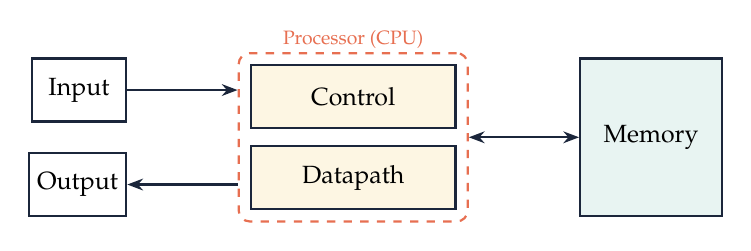
\begin{tikzpicture}[node distance=6mm and 9mm]
\node[blkg,minimum width=26mm] (ctl) {Control};
\node[blkg,minimum width=26mm,below=2mm of ctl] (dp) {Datapath};
\node[draw=coral,thick,dashed,rounded corners,inner sep=4pt,fit=(ctl)(dp),label={[tk,coral]above:Processor (CPU)}] (cpu) {};
\node[blkm,right=14mm of cpu,minimum height=20mm,minimum width=18mm] (mem) {Memory};
\node[blk,left=14mm of cpu,yshift=6mm] (in) {Input};
\node[blk,left=14mm of cpu,yshift=-6mm] (out) {Output};
\draw[wire] (in.east) -- (in.east-|cpu.west);
\draw[wire] (out.east-|cpu.west) -- (out.east);
\draw[wire,<->] (cpu.east) -- (mem.west);
\end{tikzpicture}}
\begin{itemize}
  \item \textbf{Input}: brings data and programs into the computer (keyboard, mouse, touchscreen, microphone,
        network adapter, storage devices).
  \item \textbf{Output}: sends results to the user or to other machines (display, printer, speaker, network).
  \item \textbf{Memory}: stores programs while they run and the data they need. This includes main memory
        (DRAM), caches (SRAM), and secondary storage (disk, flash) for non-volatile storage.
  \item \textbf{Datapath}: performs the arithmetic and logical operations. It holds the ALU, registers and the
        buses between them.
  \item \textbf{Control}: tells the datapath, memory and I/O what to do, according to the instruction being
        executed (it generates the control signals).
\end{itemize}
\ans{Input, Output, Memory, Datapath and Control; the datapath and control together form the processor.}
\end{solution}

%---------------------------------------------------------------- PF24
\begin{question}{2011--2012 \textbullet\ Q1(c)}{CSE 305 \textbullet\ 27/07/2013 \textbullet\ PF24}{7}
Suppose we have two implementations of the same instruction set architecture. Computer A has a clock cycle time
of 250\,ps and a CPI of 2.0 for some program, and computer B has a clock cycle time of 500\,ps and a CPI of 1.2 for
the same program. Which computer is faster for this program and by how much? (Show all steps of calculations.)
\end{question}
\begin{solution}
Same ISA and same program, so both computers execute the same instruction count $I$.
\[
\text{CPU time}=I\times\text{CPI}\times T_c
\]
\[
\text{CPU time}_A=I\times2.0\times250\text{ ps}=500\,I\text{ ps},\qquad
\text{CPU time}_B=I\times1.2\times500\text{ ps}=600\,I\text{ ps}.
\]
\[
\frac{\text{Performance}_A}{\text{Performance}_B}=\frac{\text{CPU time}_B}{\text{CPU time}_A}=\frac{600\,I}{500\,I}=1.2 .
\]
\ans{\textbf{Computer A} is faster, by a factor of \textbf{1.2}: it takes 500\,ps per instruction against B's 600\,ps.}
\end{solution}

%---------------------------------------------------------------- PF25
\begin{question}{2011--2012 \textbullet\ Q1(d)}{CSE 305 \textbullet\ 27/07/2013 \textbullet\ PF25}{6}
Suppose a program runs in 10 seconds and the program spends 50\% of its time executing floating point
instructions. We improve the floating point unit by a factor of five. How big is the speedup?
\end{question}
\begin{solution}
Amdahl's law: $T_{\text{improved}}=\dfrac{T_{\text{affected}}}{\text{improvement factor}}+T_{\text{unaffected}}$, i.e.\
$\text{Speedup}=\dfrac{1}{(1-F)+F/S}$.

Here $F=0.5$ (5\,s of FP) and $S=5$:
\[
T_{\text{new}}=\frac{5}{5}+5=6\text{ s},\qquad \text{Speedup}=\frac{10}{6}=\frac{1}{0.5+0.5/5}=1.67 .
\]
\ans{Overall speedup $=\mathbf{1.67\times}$ (10\,s $\rightarrow$ 6\,s), far below the FP unit's $5\times$. The upper bound is $1/(1-0.5)=2\times$.}
\end{solution}

%---------------------------------------------------------------- PF26
\begin{question}{2011--2012 \textbullet\ Q1(e)}{CSE 305 \textbullet\ 27/07/2013 \textbullet\ PF26}{4.5}
What are the problems with measuring performance in terms of MIPS (million instructions per second)?
\end{question}
\begin{solution}
\[
\text{MIPS}=\frac{\text{Instruction count}}{\text{Execution time}\times10^{6}}=\frac{\text{Clock rate}}{\text{CPI}\times10^{6}}
\]
MIPS is an instruction \emph{execution rate}. It does not account for:
\begin{itemize}
  \item \textbf{Differences in ISAs}: you cannot compare computers with different instruction sets, because one
        instruction does different amounts of work on each.
  \item \textbf{Differences in instruction complexity}: many simple instructions can give a high MIPS rating
        but a longer run time than fewer complex ones. Example (PF15): A rates 4000 MIPS against B's 3636, yet B
        runs the program faster (2.2\,s vs.\ 2.5\,s).
  \item \textbf{Variation of CPI between programs}: on the same CPU, MIPS changes from program to program, so a
        computer has no single MIPS rating.
\end{itemize}
In fact MIPS can even vary \emph{inversely} with performance, e.g.\ when a compiler adds cheap instructions or an
optimiser removes them.
\ans{MIPS ignores instruction count (ISA and complexity differences) and varies with the program's CPI. Use execution
time as the only reliable measure.}
\end{solution}

%===================================================================== TOPIC 02
\topic{02}{Instructions: Language of the Computer}

%---------------------------------------------------------------- IS01
\begin{question}{2023--2024 \textbullet\ Q6(b)}{CSE 209 \textbullet\ 29/04/2026 \textbullet\ IS01}{13}
Write down the MIPS assembly code for the following program.
\begin{ccode}
int main() {
    int a = 5, b = 10, c = 2;   // $t0 = a, $t1 = b, $t2 = c
    int N = 30;                 // $t3 = N
    do {
        if ((a << 2) > b) {
            a += 2;
            b += a;
        }
        else {
            a += c;
            b += c;
        }
    } while (a < N);
    return 0;
}
\end{ccode}
\end{question}
\begin{solution}
\sub{Plan}
\begin{itemize}
  \item \ins{a<<2} is one \ins{sll}. MIPS has no ``branch if greater'', so $(a\ll2) > b$ is written as $b < (a\ll2)$ with \ins{slt}, followed by \ins{beq}/\ins{bne} against \reg{zero}.
  \item A \key{do--while} tests its condition at the bottom, so the body always runs at least once.
  \item \ins{main} is a leaf procedure that only uses \reg{t} registers, so it needs no stack frame. \ins{return 0} puts 0 in \reg{v0} and returns with \ins{jr \$ra}.
\end{itemize}
\begin{mips}
main:   addi $t0, $zero, 5      # a = 5
        addi $t1, $zero, 10     # b = 10
        addi $t2, $zero, 2      # c = 2
        addi $t3, $zero, 30     # N = 30
Loop:   sll  $t4, $t0, 2        # $t4 = a << 2
        slt  $t5, $t1, $t4      # $t5 = 1 if b < (a<<2), i.e. (a<<2) > b
        beq  $t5, $zero, Else   # condition false -> else part
        addi $t0, $t0, 2        # a += 2
        add  $t1, $t1, $t0      # b += a   (uses the new a)
        j    Cond
Else:   add  $t0, $t0, $t2      # a += c
        add  $t1, $t1, $t2      # b += c
Cond:   slt  $t5, $t0, $t3      # $t5 = 1 if a < N
        bne  $t5, $zero, Loop   # repeat while (a < N)
        add  $v0, $zero, $zero  # return value 0
        jr   $ra                # return to caller
\end{mips}
\textbf{Check by tracing.} $(a,b)$ goes $(5,10)\to(7,17)\to(9,26)\to(11,37)\to(13,50)\to(15,65)\to(17,67)\to(19,86)\to(21,88)\to(23,90)\to(25,115)\to(27,117)\to(29,119)\to(31,121)$. At that point $a<N$ is false and the loop stops.
\ans{16 instructions (4 initialisations + 10-instruction loop + 2 for the return). On exit $a=31$, $b=121$ and \reg{v0}$\,=0$.}
\end{solution}

%---------------------------------------------------------------- IS02
\repeated{10}
\begin{question}{2023--2024 \textbullet\ Q6(c)}{CSE 209 \textbullet\ 29/04/2026 \textbullet\ IS02}{9}
Explain PC-relative addressing mode, Immediate addressing mode, and Base addressing mode with examples.
\end{question}
\begin{question}{2022--2023 \textbullet\ Q11(c)}{CSE 209 \textbullet\ 13/01/2025 \textbullet\ IS02}{10}
What are the different addressing modes of MIPS? Illustrate the calculation process for each addressing mode.
\end{question}
\begin{question}{2021--2022 \textbullet\ Q8(c)}{CSE 305 \textbullet\ 06/04/2023 \textbullet\ IS02}{10}
What are the different addressing modes of MIPS? Illustrate the calculation process for each addressing mode.
\end{question}
\begin{question}{2020--2021 \textbullet\ Q13(b)}{CSE 305 \textbullet\ 24/09/2022 \textbullet\ IS02}{7}
How is address calculation performed in PC-relative addressing?
\end{question}
\begin{question}{2018--2019 \textbullet\ Q6(a)}{CSE 305 \textbullet\ 29/10/2019 \textbullet\ IS02}{15}
What are the different addressing modes of MIPS? Describe and illustrate the calculation process for each addressing mode.
\end{question}
\begin{question}{2016--2017 \textbullet\ Q7(a)}{CSE 305 \textbullet\ 02/08/2017 \textbullet\ IS02}{10 + 10}
Please draw the illustrations of the five MIPS addressing modes. Also give an example instruction for each of the five addressing modes.
\end{question}
\begin{question}{2015--2016 \textbullet\ Q6(b)}{CSE 305 \textbullet\ 18/01/2017 \textbullet\ IS02}{15}
What are the different addressing modes of MIPS? Describe and illustrate the calculation process for each addressing mode.
\end{question}
\begin{question}{2014--2015 \textbullet\ Q7(a)}{CSE 305 \textbullet\ 26/01/2016 \textbullet\ IS02}{15}
Please draw the illustrations of the five MIPS addressing modes.
\end{question}
\begin{question}{2013--2014 \textbullet\ Q7(b)}{CSE 305 \textbullet\ 05/07/2015 \textbullet\ IS02}{4}
Describe MIPS addressing modes.
\end{question}
\begin{question}{2011--2012 \textbullet\ Q2(d)}{CSE 305 \textbullet\ 27/07/2013 \textbullet\ IS02}{10}
Describe MIPS addressing modes.
\end{question}
\begin{solution}
An \key{addressing mode} is the rule that tells the hardware where an instruction's operand, or its branch/jump target, is found. MIPS has \textbf{five} of them, shown below in the style of the slides' ``Addressing Mode Summary''. The 2023--24 card asks for modes 1, 3 and 4 only, and the 2020--21 card for mode 4 only, which is worked out in detail further down.

\fig{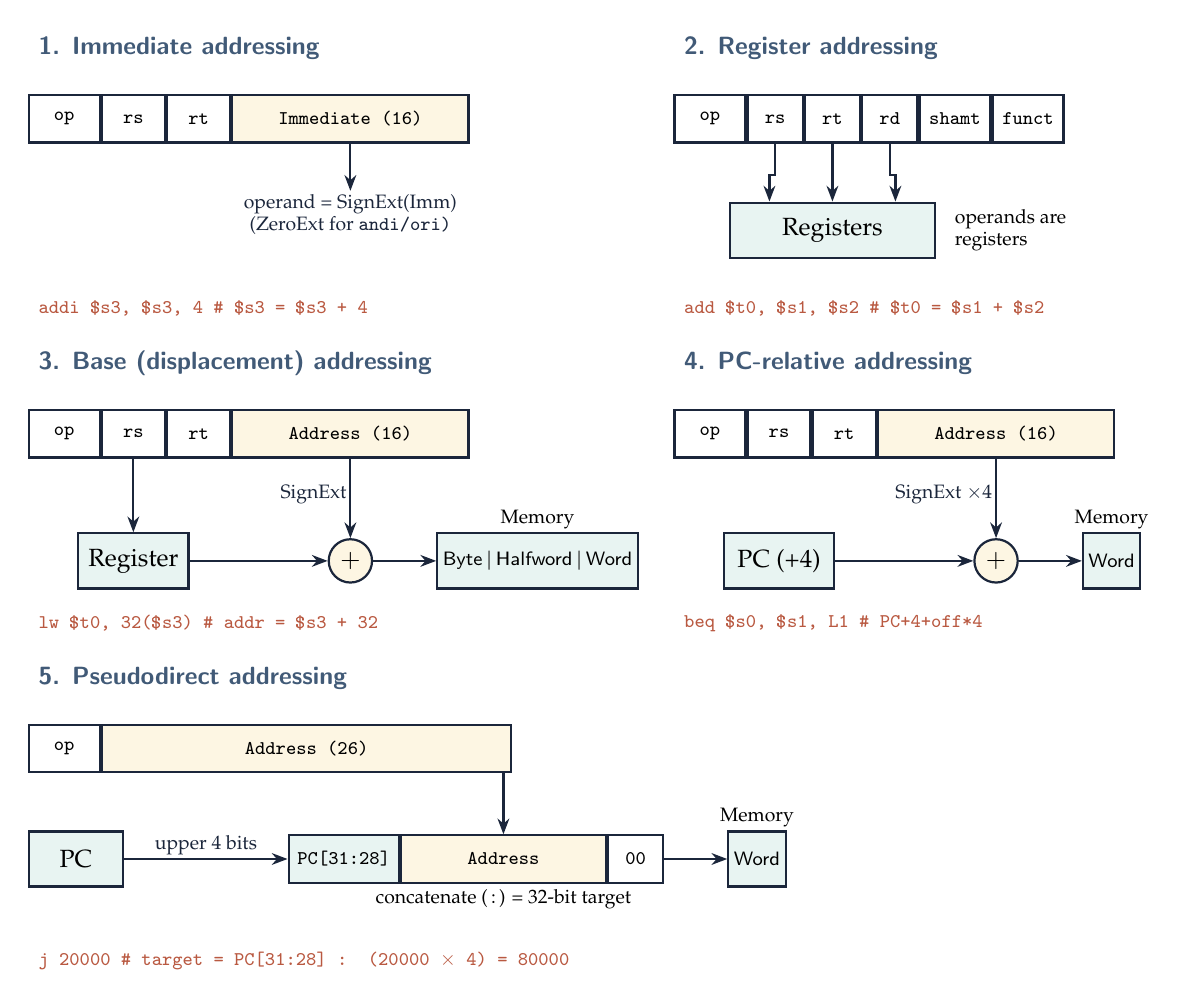
\begin{tikzpicture}[
  fld/.style={draw=ink,thick,fill=white,minimum height=6mm,font=\scriptsize\ttfamily,inner sep=1pt},
  ttl/.style={anchor=west,font=\sffamily\bfseries\small,text=inksoft},
  exm/.style={anchor=west,font=\scriptsize\ttfamily,text=coral!80!black},
  mem/.style={draw=ink,thick,fill=mist,minimum height=7mm,font=\scriptsize\sffamily,inner sep=2pt},
  sumn/.style={circle,draw=ink,thick,fill=goldbg,inner sep=0pt,minimum size=5.5mm,font=\small}]
%----------------------------------------------------- 1 immediate
\begin{scope}
\node[ttl] at (0,9mm) {1. Immediate addressing};
\node[fld,minimum width=9mm] (op1) at (4.5mm,0) {op};
\node[fld,minimum width=8mm,right=0pt of op1] (rs1) {rs};
\node[fld,minimum width=8mm,right=0pt of rs1] (rt1) {rt};
\node[fld,minimum width=30mm,fill=goldbg,right=0pt of rt1] (im1) {Immediate (16)};
\draw[wire] (im1.south) -- ++(0,-6mm) node[below,tk,align=center] {operand = SignExt(Imm)\\(ZeroExt for \ttfamily andi/ori)};
\node[exm] at (0,-24mm) {addi \$s3, \$s3, 4  \# \$s3 = \$s3 + 4};
\end{scope}
%----------------------------------------------------- 2 register
\begin{scope}[xshift=82mm]
\node[ttl] at (0,9mm) {2. Register addressing};
\node[fld,minimum width=9mm] (op2) at (4.5mm,0) {op};
\node[fld,minimum width=7mm,right=0pt of op2] (rs2) {rs};
\node[fld,minimum width=7mm,right=0pt of rs2] (rt2) {rt};
\node[fld,minimum width=7mm,right=0pt of rt2] (rd2) {rd};
\node[fld,minimum width=9mm,right=0pt of rd2] (sh2) {shamt};
\node[fld,minimum width=9mm,right=0pt of sh2] (fn2) {funct};
\node[blkm,minimum width=26mm,minimum height=7mm] (rf2) at ($(rt2.south)+(0,-11mm)$) {Registers};
\draw[wire] (rs2.south) -- ++(0,-4mm) -| ([xshift=-8mm]rf2.north);
\draw[wire] (rt2.south) -- (rf2.north);
\draw[wire] (rd2.south) -- ++(0,-4mm) -| ([xshift=8mm]rf2.north);
\node[tk,right=2mm of rf2,align=left] {operands are\\registers};
\node[exm] at (0,-24mm) {add \$t0, \$s1, \$s2  \# \$t0 = \$s1 + \$s2};
\end{scope}
%----------------------------------------------------- 3 base
\begin{scope}[yshift=-40mm]
\node[ttl] at (0,9mm) {3. Base (displacement) addressing};
\node[fld,minimum width=9mm] (op3) at (4.5mm,0) {op};
\node[fld,minimum width=8mm,right=0pt of op3] (rs3) {rs};
\node[fld,minimum width=8mm,right=0pt of rs3] (rt3) {rt};
\node[fld,minimum width=30mm,fill=goldbg,right=0pt of rt3] (ad3) {Address (16)};
\node[blkm,minimum width=14mm,minimum height=7mm] (rg3) at ($(rs3.south)+(0,-13mm)$) {Register};
\node[sumn] (s3) at ($(ad3.south)+(0,-13mm)$) {$+$};
\node[mem,right=8mm of s3] (m3) {Byte\,\textbar\,Halfword\,\textbar\,Word};
\node[tk,above=0pt of m3] {Memory};
\draw[wire] (rs3.south) -- (rg3.north);
\draw[wire] (rg3.east) -- (s3.west);
\draw[wire] (ad3.south) -- node[tk,left,pos=0.45] {SignExt} (s3.north);
\draw[wire] (s3.east) -- (m3.west);
\node[exm] at (0,-24mm) {lw \$t0, 32(\$s3)  \# addr = \$s3 + 32};
\end{scope}
%----------------------------------------------------- 4 PC-relative
\begin{scope}[xshift=82mm,yshift=-40mm]
\node[ttl] at (0,9mm) {4. PC-relative addressing};
\node[fld,minimum width=9mm] (op4) at (4.5mm,0) {op};
\node[fld,minimum width=8mm,right=0pt of op4] (rs4) {rs};
\node[fld,minimum width=8mm,right=0pt of rs4] (rt4) {rt};
\node[fld,minimum width=30mm,fill=goldbg,right=0pt of rt4] (ad4) {Address (16)};
\node[blkm,minimum width=14mm,minimum height=7mm] (pc4) at ($(rs4.south)+(0,-13mm)$) {PC (+4)};
\node[sumn] (s4) at ($(ad4.south)+(0,-13mm)$) {$+$};
\node[mem,right=8mm of s4] (m4) {Word};
\node[tk,above=0pt of m4] {Memory};
\draw[wire] (pc4.east) -- (s4.west);
\draw[wire] (ad4.south) -- node[tk,left,pos=0.45] {SignExt $\times4$} (s4.north);
\draw[wire] (s4.east) -- (m4.west);
\node[exm] at (0,-24mm) {beq \$s0, \$s1, L1  \# PC+4+off*4};
\end{scope}
%----------------------------------------------------- 5 pseudodirect
\begin{scope}[yshift=-80mm]
\node[ttl] at (0,9mm) {5. Pseudodirect addressing};
\node[fld,minimum width=9mm] (op5) at (4.5mm,0) {op};
\node[fld,minimum width=52mm,fill=goldbg,right=0pt of op5] (ad5) {Address (26)};
\node[blkm,minimum width=12mm,minimum height=7mm] (pc5) at (6mm,-14mm) {PC};
\node[fld,minimum width=14mm,fill=mist] (c1) at (40mm,-14mm) {PC[31:28]};
\node[fld,minimum width=26mm,fill=goldbg,right=0pt of c1] (c2) {Address};
\node[fld,minimum width=7mm,right=0pt of c2] (c3) {00};
\node[mem,right=8mm of c3] (m5) {Word};
\node[tk,above=0pt of m5] {Memory};
\draw[wire] (pc5.east) -- node[tk,above] {upper 4 bits} (c1.west);
\draw[wire] (ad5.south -| c2.north) -- (c2.north);
\draw[wire] (c3.east) -- (m5.west);
\node[tk,below=1pt of c2] {concatenate (\,:\,) = 32-bit target};
\node[exm] at (0,-27mm) {j 20000  \# target = PC[31:28] : (20000 $\times$ 4) = 80000};
\end{scope}
\end{tikzpicture}}

\sub{Summary and calculation process}
{\small\setlength{\tabcolsep}{4pt}
\begin{tabularx}{\linewidth}{@{}>{\raggedright\arraybackslash}p{24mm}>{\raggedright\arraybackslash}X>{\raggedright\arraybackslash}p{31mm}>{\raggedright\arraybackslash}p{29mm}@{}}
\toprule
Mode & Where the operand / target is & Example & Used by\\
\midrule
Immediate & The constant is inside the instruction (16 bits, sign-extended) & \ins{addi \$s3,\$s3,4} & \ins{addi, slti, andi, ori, lui}\\
Register & The operand is a register named by rs/rt/rd (5-bit numbers) & \ins{add \$t0,\$s1,\$s2} & R-type, \ins{jr}\\
Base & EA $=$ Reg[rs] $+$ SignExt(offset$_{16}$) & \ins{lw \$t0,32(\$s3)} & \ins{lw, sw, lb, lh, sb, ll, sc}\\
PC-relative & Target $=$ (PC$+4$) $+$ SignExt(offset$_{16}$)$\times4$ & \ins{bne \$t0,\$s5,Exit} & \ins{beq, bne}\\
Pseudodirect & Target $=$ PC$_{31..28}$ : address$_{26}$ : 00 & \ins{j Loop}, \ins{jal f} & \ins{j, jal}\\
\bottomrule
\end{tabularx}}

\sub{PC-relative addressing in detail (2020--21 card; also 2023--24)}
\begin{enumerate}
  \item While the branch is fetched, the PC has already been incremented, so the reference point is \textbf{PC$+4$}.
  \item The 16-bit offset field is a signed count of \emph{words}. It is sign-extended to 32 bits and shifted left 2 (that is, $\times4$), because instructions are word-aligned.
  \item Target $=$ (PC$+4$) $+$ SignExt(offset)$\times4$. Since offset $\in[-2^{15},\,2^{15}-1]$, a branch reaches roughly $\pm2^{15}$ instructions ($\approx\pm128$\,KB) around itself. That is enough because most branch targets are near the branch (loops, if-else).
\end{enumerate}
\textit{Example} (slides' loop at 80000): \ins{bne \$t0,\$s5,Exit} sits at 80012 and its offset field is 2, so the target is $80012+4+2\times4 = 80024$, which is \ins{Exit}.

\textit{Base example:} for \ins{lw \$t0, 32(\$s3)} with \reg{s3}$\,=\,$\hex{10010000}, EA $=$ \hex{10010000}$+32=$ \hex{10010020}. This is how \ins{A[8]} is accessed.\\
\textit{Immediate example:} \ins{addi \$s2, \$s1, -1}. The constant $-1$ (\hex{FFFF}) is sign-extended to \hex{FFFFFFFF} and added, so no load is needed. For a 32-bit constant, \ins{lui} first puts the upper 16 bits in place.
\ans{The five MIPS modes are immediate, register, base (displacement), PC-relative and pseudodirect. Branches use PC-relative addressing: target $=$ PC$+4+$SignExt(offset)$\times4$. Loads and stores use base addressing: EA $=$ rs $+$ SignExt(offset). Jumps use pseudodirect addressing: PC$_{31..28}$\,:\,addr$_{26}$\,:\,00.}
\end{solution}

%---------------------------------------------------------------- IS03
\repeated{3}
\begin{question}{2023--2024 \textbullet\ Q8(c)}{CSE 209 \textbullet\ 29/04/2026 \textbullet\ IS03}{5}
Given the following branch instruction where register \reg{s0} value equals to register \reg{s1} value and label \ins{L1} indicates an out of range branching distance. \ins{beq \$s0, \$s1, L1}.
Replace the \ins{beq} instruction by a pair of instructions that offers a much greater branching distance and resolves the out of range branching issue.
\end{question}
\begin{question}{2013--2014 \textbullet\ Q6(d)}{CSE 305 \textbullet\ 05/07/2015 \textbullet\ IS03}{3}
If branch target is too far to encode with 16-bit offset, how does the assembler rewrite the following code:
\ins{beq \$s0, \$s1, L1}
\end{question}
\begin{question}{2011--2012 \textbullet\ Q2(c)}{CSE 305 \textbullet\ 27/07/2013 \textbullet\ IS03}{3.5}
If branch target is too far to encode with 16-bit offset, how does the assembler rewrite the following code: \ins{BEQ \$s0, \$s1, L1}?
\end{question}
\begin{solution}
\sub{Why the branch can fail}
\ins{beq}/\ins{bne} are I-format instructions: \fbox{\scriptsize op\,(6)}\fbox{\scriptsize rs\,(5)}\fbox{\scriptsize rt\,(5)}\fbox{\scriptsize offset\,(16)}. They use PC-relative addressing:
\[ \text{target} = (\text{PC}+4) + \text{SignExt}(\text{offset})\times 4,\qquad -2^{15}\le \text{offset}\le 2^{15}-1 .\]
So a branch reaches only $-131072$ to $+131068$ bytes ($\pm2^{15}$ words) from PC$+4$. If \ins{L1} lies farther away, the offset does not fit in 16 bits.

\sub{The rewrite (slides: ``Branching far away'')}
Invert the condition and branch a short distance over an unconditional \ins{j}. The \ins{j} instruction has a 26-bit word address, so it reaches anywhere in the current 256\,MB region (target $=$ PC$_{31..28}$:addr$_{26}$:00).
\fig{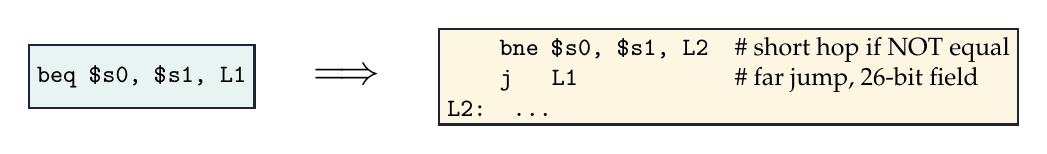
\begin{tikzpicture}[font=\small]
\node[blkm,font=\ttfamily\small] (a) {beq \$s0, \$s1, L1};
\node[right=6mm of a] (ar) {\Large$\Longrightarrow$};
\node[blkg,font=\ttfamily\small,align=left,right=6mm of ar] (b) {\phantom{L2:\ }bne \$s0, \$s1, L2\ \ \textrm{\# short hop if NOT equal}\\\phantom{L2:\ }j\ \ \ L1\ \ \ \ \ \ \ \ \ \ \ \ \textrm{\# far jump, 26-bit field}\\L2:\ \ ...};
\end{tikzpicture}}
When \reg{s0}$=$\reg{s1} (the case in the 2023--24 card), \ins{bne} falls through and \ins{j} takes control to \ins{L1}, exactly as the original \ins{beq} would. When they differ, execution continues at \ins{L2}, the instruction that followed the original \ins{beq}.
\ans{\ins{bne \$s0, \$s1, L2}; \ins{j L1}; \ins{L2: \ldots}. The inverted short branch skips over a pseudodirect jump that can reach the whole 256\,MB region.}
\end{solution}

%---------------------------------------------------------------- IS04
\begin{question}{2022--2023 \textbullet\ Q6}{CSE 209 \textbullet\ 13/01/2025 \textbullet\ IS04}{15}
The current implementation of MIPS hardware doesn't support memory values as operand for R-type instructions. You can perform R-type instructions only if both of the operand values are stored in a register. Now you want to add a new instruction type (i.e.\ M-type instruction).

In M-type instruction you should perform only addition and subtraction, where one of the operand value would be stored in the memory (i.e.\ memory operand).

Now you need to design the M-type instruction format (i.e.\ which bits will represent which value) and the conversion protocol for transforming MIPS assembly to machine code for M-type instruction. You have the full freedom to design the new format and you can set any rules you wish; you can add new control signal(s) if needed. Explain your designed instruction format with proper justification. While designing your new protocol you \textbf{mustn't} hamper the working of the three original instruction formats.

Also, there will be major change(s) needed in hardware for the above-described M-type instruction. Identify the change(s) and explain them with proper justification.
\end{question}
\begin{solution}
\sub{1. Semantics and assembly syntax (one possible design)}
\begin{gather*}
\texttt{addm rd, rt, offset(rs)}:\quad \texttt{rd} \leftarrow \texttt{rt} + \text{Mem}[\texttt{rs}+\text{SignExt(offset)}]\\
\texttt{subm rd, rt, offset(rs)}:\quad \texttt{rd} \leftarrow \texttt{rt} - \text{Mem}[\texttt{rs}+\text{SignExt(offset)}]
\end{gather*}
This keeps the three-operand style (\emph{simplicity favours regularity}) and uses the same \ins{offset(base)} notation as \ins{lw}/\ins{sw}.

\sub{2. M-type format (32 bits)}
\fig{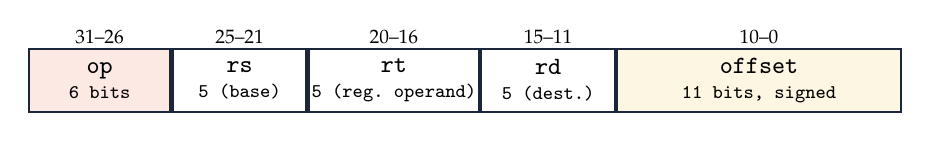
\begin{tikzpicture}[fld/.style={draw=ink,thick,minimum height=8mm,font=\small\ttfamily,align=center,inner sep=1pt}]
\node[fld,fill=rose,minimum width=18mm] (o) {op\\[-2pt]{\scriptsize 6 bits}};
\node[fld,fill=white,minimum width=17mm,right=0pt of o] (s) {rs\\[-2pt]{\scriptsize 5 (base)}};
\node[fld,fill=white,minimum width=17mm,right=0pt of s] (t) {rt\\[-2pt]{\scriptsize 5 (reg.\ operand)}};
\node[fld,fill=white,minimum width=17mm,right=0pt of t] (d) {rd\\[-2pt]{\scriptsize 5 (dest.)}};
\node[fld,fill=goldbg,minimum width=36mm,right=0pt of d] (f) {offset\\[-2pt]{\scriptsize 11 bits, signed}};
\foreach \n/\l in {o/31--26,s/25--21,t/20--16,d/15--11,f/10--0}{\node[tk,above=0pt of \n]{\l};}
\end{tikzpicture}}
\textbf{Justification}
\begin{itemize}
  \item \textbf{rs and rt sit in bits 25--21 and 20--16}, as in R- and I-format, and \textbf{rd in 15--11}, as in R-format. The register file can therefore be read before decoding finishes, and the existing RegDst mux already selects rd (\emph{good design demands good compromises}: keep formats as similar as possible).
  \item \textbf{add vs.\ sub is told apart by the opcode} (two new, currently unused opcodes, e.g.\ \texttt{24}~$=$~\ins{addm}, \texttt{25}~$=$~\ins{subm}) rather than by a funct field. This leaves $32-6-15=11$ bits for the offset (range $-1024\ldots+1023$ bytes).
  \item \textbf{Original formats are untouched}: R (op$=$0), I and J instructions keep their opcodes and fields. Only the control unit learns two more opcodes.
\end{itemize}

\sub{3. Conversion protocol (assembler rules)}
\begin{enumerate}
  \item Mnemonic $\to$ opcode: \ins{addm}$\to$\texttt{011000}, \ins{subm}$\to$\texttt{011001}.
  \item The 1st register is rd, the 2nd is rt, and the register in parentheses is rs. Each is written as its 5-bit number.
  \item The offset is a byte offset written as 11-bit two's complement. It must be a multiple of 4 (word operand). If it lies outside $[-1024,1023]$, the assembler expands the instruction into \ins{lw \$at,off(rs)} and \ins{add/sub rd,rt,\$at}, the same way pseudoinstructions are handled.
\end{enumerate}
\textit{Example:} \ins{addm \$t0, \$s1, 8(\$s2)} $\to$ op$=24$, rs$=18$, rt$=17$, rd$=8$, offset$=8$:
\[\texttt{011000\ 10010\ 10001\ 01000\ 00000001000} = \texttt{0x62514008}.\]
Similarly, \ins{subm \$t0,\$s1,-4(\$s2)} has offset field \texttt{11111111100} and encodes as \hex{665147FC}.

\sub{4. Hardware changes}
\fig{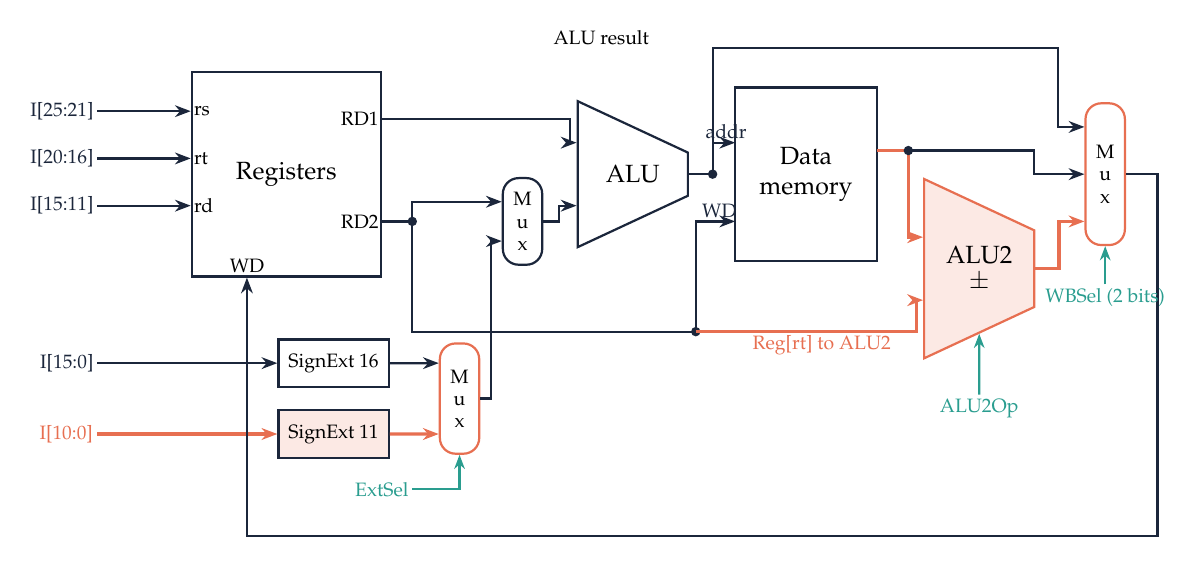
\begin{tikzpicture}[font=\small]
\node[blk,minimum width=24mm,minimum height=26mm,align=center] (rf) at (0,0) {Registers};
\node[tk,anchor=west] at ([yshift=8mm]rf.west) {rs};
\node[tk,anchor=west] at ([yshift=2mm]rf.west) {rt};
\node[tk,anchor=west] at ([yshift=-4mm]rf.west) {rd};
\node[tk,above=0.5pt] at ([xshift=-5mm]rf.south) {WD};
\node[tk,anchor=east] at ([yshift=7mm]rf.east) {RD1};
\node[tk,anchor=east] at ([yshift=-6mm]rf.east) {RD2};
\draw[wire] (-24mm,8mm) node[left,tk]{I[25:21]} -- ([yshift=8mm]rf.west);
\draw[wire] (-24mm,2mm) node[left,tk]{I[20:16]} -- ([yshift=2mm]rf.west);
\draw[wire] (-24mm,-4mm) node[left,tk]{I[15:11]} -- ([yshift=-4mm]rf.west);
\node[blk,minimum width=14mm,minimum height=6mm,font=\scriptsize] (se16) at (6mm,-24mm) {SignExt 16};
\node[blkr,minimum width=14mm,minimum height=6mm,font=\scriptsize] (se11) at (6mm,-33mm) {SignExt 11};
\draw[wire] (-24mm,-24mm) node[left,tk]{I[15:0]} -- (se16.west);
\draw[newwire] (-24mm,-33mm) node[left,tk]{I[10:0]} -- (se11.west);
\node[muxs,rectangle,rounded corners=2mm,draw=coral,minimum height=14mm] (xm) at (22mm,-28.5mm) {M\\u\\x};
\draw[wire] (se16.east) -- ([yshift=4.5mm]xm.west);
\draw[newwire] (se11.east) -- ([yshift=-4.5mm]xm.west);
\node[muxs,rectangle,rounded corners=2mm] (as) at (30mm,-6mm) {M\\u\\x};
\draw[wire] (12mm,-6mm) -- (16mm,-6mm) |- ([yshift=2.5mm]as.west);
\fill[ink] (16mm,-6mm) circle (0.6mm);
\draw[wire] (xm.east) -- (26mm,-28.5mm) |- ([yshift=-2.5mm]as.west);
\node[alu] (alu) at (44mm,0) {ALU};
\draw[wire] (12mm,7mm) -- (36mm,7mm) |- ([yshift=4mm]alu.west);
\draw[wire] (as.east) -- ++(2mm,0) |- ([yshift=-4mm]alu.west);
\coordinate (j1) at ($(alu.east)+(3mm,0)$);
\coordinate (top) at (0,16mm);
\node[blk,minimum width=18mm,minimum height=22mm,align=center] (dm) at (66mm,0) {Data\\memory};
\draw[wire] (alu.east) -- (j1) |- node[tk,above,pos=0.8]{addr} (57mm,4mm);
\fill[ink] (j1) circle (0.6mm);
\draw[wire] (16mm,-6mm) -- (16mm,-20mm) -- (52mm,-20mm) |- node[tk,above,pos=0.8]{WD} (57mm,-6mm);
\node[alu,draw=coral,fill=rose,align=center] (alu2) at (88mm,-12mm) {ALU2\\[-2pt]$\pm$};
\draw[newwire] (75mm,3mm) -- (79mm,3mm) |- ([yshift=4mm]alu2.west);
\fill[ink] (79mm,3mm) circle (0.6mm);
\fill[ink] (52mm,-20mm) circle (0.6mm);
\draw[newwire] (52mm,-20mm) -- (80mm,-20mm) |- ([yshift=-4mm]alu2.west);
\node[tk,text=coral,below] at (68mm,-20mm) {Reg[rt] to ALU2};
\node[muxs,rectangle,rounded corners=2mm,draw=coral,minimum height=18mm] (wb) at (104mm,0) {M\\u\\x};
\draw[wire] (j1) -- (j1 |- top) -| (98mm,6mm) -- ([yshift=6mm]wb.west);
\draw[wire] (79mm,3mm) -- (95mm,3mm) |- (wb.west);
\draw[newwire] (alu2.east) -- ++(3mm,0) |- ([yshift=-6mm]wb.west);
\draw[wire] (wb.east) -- ++(4mm,0) |- (-5mm,-46mm) -- ([xshift=-5mm]rf.south);
\draw[ctl] (88mm,-28mm) node[below,tk,text=teal]{ALU2Op} -- (alu2.south);
\draw[ctl] (16mm,-40mm) node[left,tk,text=teal]{ExtSel} -| (xm.south);
\draw[ctl] (104mm,-14mm) node[below,tk,text=teal]{WBSel (2 bits)} -- (wb.south);
\node[tk,above] at (40mm,16mm) {ALU result};
\end{tikzpicture}}
\begin{enumerate}
  \item \textbf{Second arithmetic unit (ALU2, add/sub) after data memory.} In a single-cycle datapath the main ALU is busy computing the address rs$+$offset in the same cycle, so the memory operand needs its own adder/subtractor. Its inputs are Mem[EA] and Reg[rt] (Read data 2, which until now went only to memory for \ins{sw}).
  \item \textbf{Write-back mux widened to 3 inputs} (ALU result / memory data / ALU2 result). MemtoReg becomes a 2-bit signal, \textsf{WBSel}.
  \item \textbf{11-bit sign extender plus a mux} (\textsf{ExtSel}), so the address offset comes from bits 10--0 for M-type and from bits 15--0 for I-type.
  \item \textbf{Control unit:} it decodes the two new opcodes and generates RegDst$=1$, ALUSrc$=1$, ALUOp$=$add, MemRead$=1$, MemWrite$=0$, RegWrite$=1$, ExtSel$=1$, WBSel$=$ALU2, ALU2Op$=0$ (\ins{addm}) or $1$ (\ins{subm}). All existing instructions get ExtSel$=0$ and their old WBSel values, so their behaviour does not change.
  \item \textbf{Timing:} the critical path becomes IM $\to$ Reg $\to$ ALU $\to$ DM $\to$ ALU2 $\to$ Reg, longer than \ins{lw}'s. In a single-cycle design \emph{every} instruction pays for this longer clock. In a pipeline it would need an extra stage (or a memory-then-execute ordering, as in x86-style pipelines) and extra forwarding and stall logic. This is exactly why load/store RISC ISAs avoid memory operands.
\end{enumerate}
\ans{Format: op(6) $|$ rs(5, base) $|$ rt(5, register operand) $|$ rd(5, destination) $|$ offset(11, signed), with opcodes 24/25 for \ins{addm}/\ins{subm}. Meaning: rd $=$ rt $\pm$ Mem[rs $+$ SignExt(offset)]. Hardware: a second add/sub unit after data memory, a 3-input write-back mux (WBSel), an 11-bit sign extender with its select mux (ExtSel), new control outputs, and a longer critical path.}
\end{solution}

%---------------------------------------------------------------- IS05
\begin{question}{2022--2023 \textbullet\ Q9(c)}{CSE 209 \textbullet\ 13/01/2025 \textbullet\ IS05}{10}
Convert the code snippet below to the MIPS assembly code.
\begin{center}\small Listing 1: Code Snippet for Question 9(c)\end{center}
\begin{ccode}[numbers=left,numberstyle=\scriptsize]
int fun(int a, int b){
    if (b == 0) return 0;
    else if (b / 2 == 0) return fun(a*4, b/8);
    return fun(a+a, b/4) + a;
}
\end{ccode}
\end{question}
\begin{solution}
\sub{Method}
\begin{itemize}
  \item Arguments: \ins{a} in \reg{a0}, \ins{b} in \reg{a1}. The result goes in \reg{v0}.
  \item Multiplying or dividing by a power of two becomes a shift: \ins{a*4} $\to$ \ins{sll 2}, \ins{b/2}, \ins{b/4}, \ins{b/8} $\to$ \ins{sra 1/2/3}. We assume $b\ge0$, so \ins{sra} gives the same result as C's truncating division.
  \item \ins{return fun(a*4, b/8)} returns the callee's value \emph{unchanged}. It can therefore be a \textbf{tail call}: set up the new arguments and \ins{j fun}. \reg{ra} still holds the original caller's address, so no stack frame is needed.
  \item \ins{fun(a+a, b/4) + a} still needs \ins{a} after the call, so that path is non-leaf. It saves \reg{ra} and \ins{a} on the stack, calls with \ins{jal}, then restores both (slides: non-leaf procedure).
\end{itemize}
\begin{mips}
fun:   bne  $a1, $zero, L1      # if (b == 0)
       add  $v0, $zero, $zero   #     return 0
       jr   $ra
L1:    sra  $t0, $a1, 1         # $t0 = b / 2
       bne  $t0, $zero, L2      # else if (b/2 == 0) ...
       sll  $a0, $a0, 2         #   a = a*4
       sra  $a1, $a1, 3         #   b = b/8
       j    fun                 #   return fun(a*4, b/8)   (tail call)
L2:    addi $sp, $sp, -8        # non-leaf part: make a 2-word frame
       sw   $ra, 4($sp)         # save return address
       sw   $a0, 0($sp)         # save a (needed after the call)
       add  $a0, $a0, $a0       # 1st arg = a + a
       sra  $a1, $a1, 2         # 2nd arg = b / 4
       jal  fun                 # $v0 = fun(a+a, b/4)
       lw   $a0, 0($sp)         # restore a
       lw   $ra, 4($sp)         # restore return address
       addi $sp, $sp, 8         # pop frame
       add  $v0, $v0, $a0       # return fun(a+a, b/4) + a
       jr   $ra
\end{mips}
(A conventional \ins{jal fun} with its own stack frame in place of the tail \ins{j fun} is also correct, just longer.)\\
\textit{Check:} \ins{fun(3,5)} $=$ \ins{fun(6,1)}$+3$. \ins{fun(6,1)}: $1/2=0$, so it returns \ins{fun(24,0)}$\,=0$. Hence the result is $3$, which the code also gives.
\ans{The 19-instruction procedure above. Shifts replace \ins{*4}, \ins{/2}, \ins{/4} and \ins{/8}. \ins{fun(a*4,b/8)} is a tail jump. Only the \ins{fun(a+a,b/4)+a} path builds a 2-word stack frame holding \reg{ra} and \ins{a}.}
\end{solution}

%---------------------------------------------------------------- IS06
\begin{question}{2022--2023 \textbullet\ Q11(b)}{CSE 209 \textbullet\ 13/01/2025 \textbullet\ IS06}{8}
How does ``\ins{jal}'' instruction differ from an unconditional jump instruction? How is the NOT operation performed in the MIPS assembly language?
\end{question}
\begin{solution}
\sub{\ins{jal} vs.\ \ins{j}}
{\small\begin{tabularx}{\linewidth}{@{}>{\raggedright\arraybackslash}p{30mm}>{\raggedright\arraybackslash}X>{\raggedright\arraybackslash}X@{}}
\toprule
 & \ins{j Label} (jump) & \ins{jal Label} (jump and link)\\
\midrule
Format / opcode & J-format, op $=2$, 26-bit address & J-format, op $=3$, 26-bit address\\
Target & PC $\leftarrow$ PC$_{31..28}$ : addr : 00 & same target computation\\
Side effect & none & \reg{ra} (reg 31) $\leftarrow$ PC$+4$, the return address\\
Purpose & \texttt{goto}, end of if-else, loop back-edge & \textbf{procedure call}. The callee returns with \ins{jr \$ra}\\
\bottomrule
\end{tabularx}}
So \ins{jal} is an unconditional jump that also \emph{links}: it saves the address of the next instruction so control can come back to the caller. A non-leaf procedure must save \reg{ra} on the stack before its own \ins{jal}, because the new \ins{jal} overwrites it.
\begin{mips}
      jal  leaf         # $ra = address of next instr; PC = leaf
      ...               # execution resumes here after the return
leaf: ...
      jr   $ra          # PC = $ra  -> back to caller
\end{mips}

\sub{NOT in MIPS}
MIPS has no \ins{not} instruction. It uses the 3-operand \ins{nor}, since $a \textsf{ NOR } 0 = \overline{a+0} = \overline{a}$ (slides: ``NOT Operations''):
\begin{mips}
nor $t0, $t1, $zero     # $t0 = ~$t1
\end{mips}
Example:
\fig{\begin{tabular}{rl}
\reg{t1} $=$ & \texttt{0000 0000 0000 0000 0011 1100 0000 0000}\\
\reg{t0} $=$ \ins{nor}(\reg{t1}, 0) $=$ & \texttt{1111 1111 1111 1111 1100 0011 1111 1111}
\end{tabular}}
The assembler pseudoinstruction \ins{not \$t0,\$t1} expands to exactly this \ins{nor}. \ins{xori \$t0,\$t1,0xFFFF} would \emph{not} work, because \ins{xori} zero-extends its immediate and so inverts only the low 16 bits.
\ans{\ins{jal} jumps like \ins{j} but also stores PC$+4$ in \reg{ra}, so a procedure can return with \ins{jr \$ra}. \ins{j} only changes the PC. NOT is done with \ins{nor rd, rs, \$zero}.}
\end{solution}

%---------------------------------------------------------------- IS07
\repeated{3}
\begin{question}{2022--2023 \textbullet\ Q12(a--b)}{CSE 209 \textbullet\ 13/01/2025 \textbullet\ IS07}{5 + 10}
\textbf{(a)} How does Just-In-Time (JIT) compilation improve the performance of a Java application? \hfill(5)\\
\textbf{(b)} What is the main difference between static linking and dynamic linking? What are the advantages of using dynamic linking? \hfill(10)
\end{question}
\begin{question}{2022--2023 \textbullet\ Q7(d)}{CSE 305 \textbullet\ 25/04/2024 \textbullet\ IS07}{15}
Write about the main difference between static linking and dynamic linking. With the necessary diagrams, explain how dynamically linked libraries (DLLs) are called.
\end{question}
\begin{question}{2019--2020 \textbullet\ Q1(c)}{CSE 305 \textbullet\ 18/09/2021 \textbullet\ IS07}{4 + 4}
What are the advantages of using Dynamically Linked Libraries (DLL) during a C program execution? What is the role of JIT in Java program execution?
\end{question}
\begin{solution}
\sub{Static vs.\ dynamic linking (main difference)}
{\small\begin{tabularx}{\linewidth}{@{}>{\raggedright\arraybackslash}p{24mm}>{\raggedright\arraybackslash}X>{\raggedright\arraybackslash}X@{}}
\toprule
 & Static linking & Dynamic linking (DLL / shared library)\\
\midrule
When & Before execution. The linker merges all object modules \emph{and} every referenced library routine into one executable. & At load time or at run time. A library routine is linked and loaded only when it is (first) called.\\
Executable & Large: it contains copies of all library code, called or not. & Small: it contains only references (stubs) to the library.\\
Library update & Program keeps the old version until it is re-linked. & The new library version is picked up automatically.\\
Requirement & none & Library code must be relocatable. There is some extra overhead on the first call.\\
\bottomrule
\end{tabularx}}

\sub{Advantages of dynamic linking / DLLs (2022--23 Q12(b), 2019--20)}
\begin{itemize}
  \item \textbf{No image bloat:} only routines that are actually called are loaded. Static linking pulls in all (transitively) referenced libraries.
  \item \textbf{Automatic upgrades and bug fixes:} a new library version is used without re-linking the program.
  \item \textbf{Sharing:} one copy of a DLL in memory can serve many running programs, which saves memory and disk.
  \item \textbf{Faster start-up with lazy linkage:} a routine is resolved only on its first call, so unused routines cost nothing.
\end{itemize}

\sub{How a DLL routine is called: lazy procedure linkage (2022--23 Q7(d))}
\fig{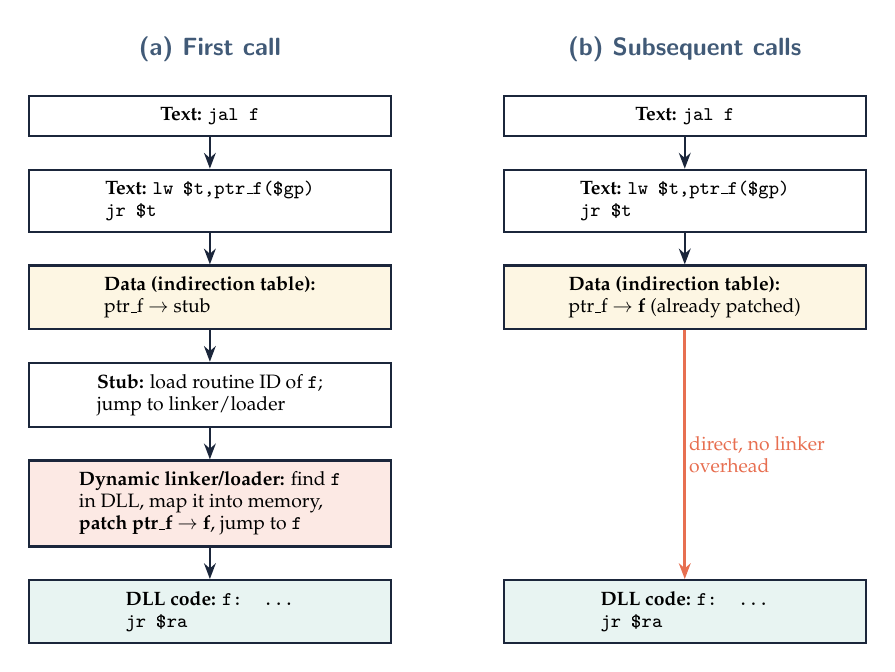
\begin{tikzpicture}[node distance=4mm,font=\small,
  b/.style={proc,minimum width=46mm,font=\scriptsize,align=left},
  hd/.style={font=\sffamily\bfseries\small,text=inksoft}]
\node[hd] (ha) {(a) First call};
\node[b,below=3mm of ha] (a1) {\textbf{Text:} \ttfamily jal f};
\node[b,below=of a1] (a2) {\textbf{Text:} \ttfamily lw \$t,ptr\_f(\$gp)\\\ttfamily jr \$t};
\node[b,fill=goldbg,below=of a2] (a3) {\textbf{Data (indirection table):}\\ptr\_f $\to$ stub};
\node[b,below=of a3] (a4) {\textbf{Stub:} load routine ID of \texttt{f};\\jump to linker/loader};
\node[b,fill=rose,below=of a4] (a5) {\textbf{Dynamic linker/loader:} find \texttt{f}\\in DLL, map it into memory,\\\textbf{patch ptr\_f $\to$ f}, jump to \texttt{f}};
\node[b,fill=mist,below=of a5] (a6) {\textbf{DLL code:} \texttt{f: \ldots}\\\ttfamily jr \$ra};
\foreach \u/\v in {a1/a2,a2/a3,a3/a4,a4/a5,a5/a6}{\draw[wire] (\u)--(\v);}
\node[hd,right=34mm of ha] (hb) {(b) Subsequent calls};
\node[b,below=3mm of hb] (b1) {\textbf{Text:} \ttfamily jal f};
\node[b,below=of b1] (b2) {\textbf{Text:} \ttfamily lw \$t,ptr\_f(\$gp)\\\ttfamily jr \$t};
\node[b,fill=goldbg,below=of b2] (b3) {\textbf{Data (indirection table):}\\ptr\_f $\to$ \textbf{f} (already patched)};
\node[b,fill=mist] (b6) at (b3 |- a6) {\textbf{DLL code:} \texttt{f: \ldots}\\\ttfamily jr \$ra};
\foreach \u/\v in {b1/b2,b2/b3}{\draw[wire] (\u)--(\v);}
\draw[newwire] (b3) -- node[tk,right,text=coral,align=left]{direct, no linker\\overhead} (b6);
\end{tikzpicture}}
\begin{enumerate}
  \item The program calls a DLL routine through an \key{indirection table} entry (one word per external routine). At first every entry points to a small \key{stub}.
  \item \textbf{First call:} \ins{jal} $\to$ load the pointer and \ins{jr} $\to$ stub. The stub loads the routine's ID and jumps to the \textbf{dynamic linker/loader}. The linker finds the routine, maps it into the address space, \emph{overwrites the indirection entry with the routine's real address}, and jumps to it.
  \item \textbf{Every later call:} the indirection word already holds the routine's address, so the call reaches the DLL code with only one extra indirect jump.
\end{enumerate}

\sub{Role of JIT in Java (2022--23 Q12(a), 2019--20)}
\fig{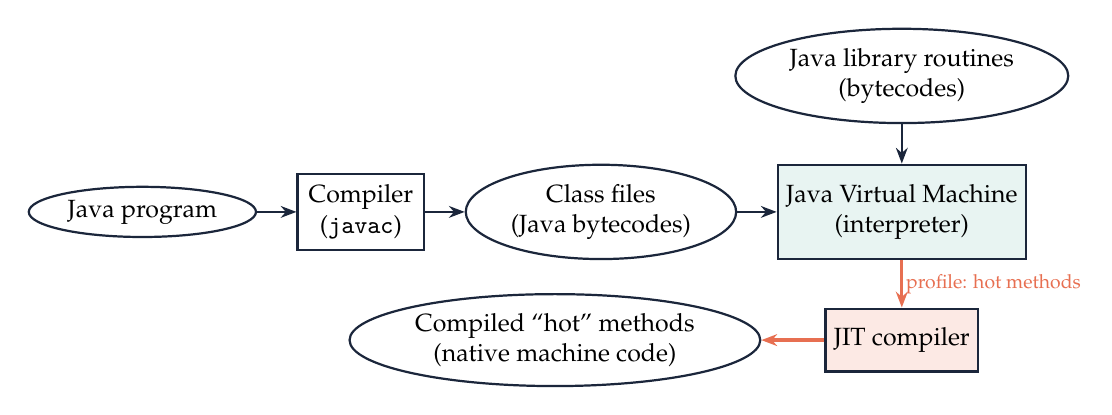
\begin{tikzpicture}[node distance=5mm,font=\small]
\node[oval] (j) {Java program};
\node[proc,right=of j] (c) {Compiler\\(\texttt{javac})};
\node[oval,right=of c] (cf) {Class files\\(Java bytecodes)};
\node[blkm,right=of cf,minimum height=12mm] (jvm) {Java Virtual Machine\\(interpreter)};
\node[oval,above=5mm of jvm] (lib) {Java library routines\\(bytecodes)};
\node[blkr,below=6mm of jvm] (jit) {JIT compiler};
\node[oval,left=8mm of jit] (nat) {Compiled ``hot'' methods\\(native machine code)};
\draw[wire] (j)--(c); \draw[wire] (c)--(cf); \draw[wire] (cf)--(jvm); \draw[wire] (lib)--(jvm);
\draw[newwire] (jvm)--node[tk,right]{profile: hot methods}(jit); \draw[newwire] (jit)--(nat);
\end{tikzpicture}}
\begin{itemize}
  \item Java is compiled to portable \textbf{bytecodes}, which the JVM normally \emph{interprets}. Interpretation is portable but slow, because every bytecode is decoded in software each time it runs.
  \item A \key{Just-In-Time compiler} profiles the running program, finds the frequently executed (``hot'') methods, and compiles their bytecodes into \textbf{native machine code} for the host machine while the program runs. The compiled code is cached and reused on later calls.
  \item Result: portability is kept, and the hot code runs at nearly compiled speed. Programs get faster the longer they run, since more of the run time is spent in native code. Only rarely used code stays interpreted.
\end{itemize}
\ans{Static linking copies all library code into the executable before it runs. Dynamic linking links each library routine only when it is loaded or first called, using an indirection table, a stub and the dynamic linker (lazy linkage). The result is smaller images, shared memory and automatic library updates. JIT speeds up Java by compiling hot bytecode methods into native code at run time instead of interpreting them.}
\end{solution}

%---------------------------------------------------------------- IS08
\begin{question}{2022--2023 \textbullet\ Q12(c)}{CSE 209 \textbullet\ 13/01/2025 \textbullet\ IS08}{10}
\begin{enumerate}
  \item Write the MIPS assembly code that creates the 32-bit constant \texttt{0010 0000 0000 0001 0100 1001 0010 0100}$_2$ and stores that value to register \reg{t1}.
  \item If the current value of the PC is \hex{00000000} can you use a single jump instruction to go to the address equal to the constant shown in question 12(c)(i)?
  \item If the current value of the PC is \hex{1FFFF000}, can you use a single branch instruction to go to the address equal to the constant shown in Question 12(c)(i)?
\end{enumerate}
\end{question}
\begin{solution}
\sub{Facts used}
\begin{itemize}
  \item 32-bit constant: \ins{lui} loads the upper 16 bits (and clears the lower half). Then \ins{ori} ORs in the lower 16 bits. \ins{ori} zero-extends its immediate, so the upper half is not disturbed.
  \item \ins{j} (pseudodirect): target $=$ (PC$+4$)$_{31..28}$ : addr$_{26}$ : 00. It can only reach addresses in the same 256\,MB region, i.e.\ with the same upper 4 bits.
  \item \ins{beq}/\ins{bne} (PC-relative): target $=$ PC$+4+$SignExt(off$_{16}$)$\times4$ with $-32768\le$ off $\le32767$.
\end{itemize}
\textbf{(i)} \texttt{0010 0000 0000 0001 \textbar\ 0100 1001 0010 0100} $=$ \hex{2001}\,\texttt{4924}. The upper half is \hex{2001} $=8193$ and the lower half is \hex{4924} $=18724$.
\begin{mips}
lui  $t1, 0x2001          # $t1 = 0x2001 0000
ori  $t1, $t1, 0x4924     # $t1 = 0x2001 4924
\end{mips}
\fig{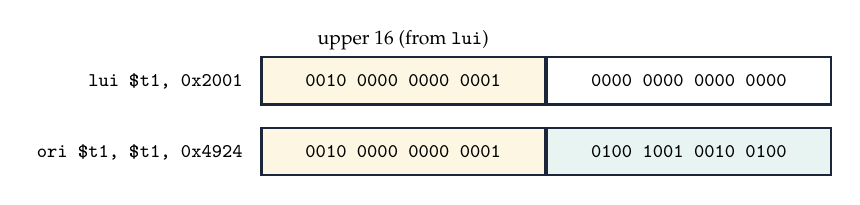
\begin{tikzpicture}[f/.style={draw=ink,thick,minimum height=6mm,minimum width=36mm,font=\scriptsize\ttfamily}]
\node[anchor=east,font=\scriptsize\ttfamily] at (-1mm,0) {lui \$t1, 0x2001};
\node[f,fill=goldbg,anchor=west] (u1) at (0,0) {0010 0000 0000 0001};
\node[f,right=0pt of u1] {0000 0000 0000 0000};
\node[anchor=east,font=\scriptsize\ttfamily] at (-1mm,-9mm) {ori \$t1, \$t1, 0x4924};
\node[f,fill=goldbg,anchor=west] (u2) at (0,-9mm) {0010 0000 0000 0001};
\node[f,fill=mist,right=0pt of u2] {0100 1001 0010 0100};
\node[tk,above=1pt of u1] {upper 16 (from \texttt{lui})};
\end{tikzpicture}}
\textbf{(ii)} PC $=$ \hex{00000000}, so PC$+4=$ \hex{00000004}, whose upper 4 bits are \texttt{0000}. The target \hex{20014924} has upper 4 bits \texttt{0010}. A \ins{j} can only produce addresses whose top 4 bits are \texttt{0000}, so \textbf{no}. (The target is word-aligned; the region is the problem.) Instead use the \ins{lui}/\ins{ori} of (i) followed by \ins{jr \$t1}.\\
\textbf{(iii)} PC$+4=$ \hex{1FFFF004}.
\[\text{offset}=\frac{\texttt{0x20014924}-\texttt{0x1FFFF004}}{4}=\frac{\texttt{0x15920}}{4}=\frac{88352}{4}=22088\ (\texttt{0x5648}) \le 2^{15}-1=32767 .\]
So \textbf{yes}: a single \ins{beq} with offset field 22088 reaches it. (A \ins{j} would fail here, because the upper bits \texttt{0001} and \texttt{0010} differ.)
\ans{(i) \ins{lui \$t1,0x2001}; \ins{ori \$t1,\$t1,0x4924}. (ii) No: the jump cannot change the upper 4 bits from 0000 to 0010. (iii) Yes: the offset is 22088, which is at most 32767.}
\end{solution}

%---------------------------------------------------------------- IS09
\begin{question}{2022--2023 \textbullet\ Q5(a)}{CSE 305 \textbullet\ 25/04/2024 \textbullet\ IS09}{7}
Rachel has a basic MIPS instruction set without support for multiple languages. In an attempt to add such support, she introduces four new instructions: \ins{lh} (load halfword), \ins{lhu} (load halfword unsigned), \ins{sh} (store halfword), and \ins{shu} (store halfword unsigned). However, Ross argued that she doesn't need all these instructions to achieve multi-language support. Do you agree with Ross? Justify your answer.
\end{question}
\begin{solution}
\textbf{Yes, I agree with Ross.} Multi-language text uses \textbf{Unicode} (UTF-16), whose characters are 16-bit \emph{halfwords} (slides: ``Character Data'', ``Byte/Halfword Operations''). Loads and stores behave differently:
\begin{itemize}
  \item \textbf{Loads widen} a 16-bit value into a 32-bit register, so the upper 16 bits must be filled somehow. \ins{lh} \emph{sign}-extends and \ins{lhu} \emph{zero}-extends. Both variants are meaningful:
  \fig{\begin{tabular}{lll}
  memory halfword \hex{8041} & \ins{lh} $\to$ \hex{FFFF8041} ($-32703$) & \ins{lhu} $\to$ \hex{00008041} ($32833$)\end{tabular}}
  \item \textbf{Stores narrow:} \ins{sh} simply writes the rightmost 16 bits of the register to memory. No extension happens, so signed and unsigned stores would write identical bits. \textbf{\ins{shu} is redundant}, which is why real MIPS has \ins{sh} but no \ins{shu}.
  \item Character codes are unsigned, so text handling really needs only \ins{lhu} (read a character) and \ins{sh} (write a character). \ins{lh} is useful for signed 16-bit integer data, not for characters. It could even be emulated as \ins{lhu}, \ins{sll 16}, \ins{sra 16}.
\end{itemize}
\ans{Agree. \ins{shu} is pointless because a store writes the same 16 bits whether the value is signed or unsigned. For Unicode text, \ins{lhu} and \ins{sh} suffice. \ins{lh} is optional and only needed for signed halfword data. So she needs 2 (at most 3) of the 4 instructions, as in real MIPS: \ins{lh}, \ins{lhu}, \ins{sh}.}
\end{solution}

%---------------------------------------------------------------- IS10
\begin{question}{2022--2023 \textbullet\ Q5(c)}{CSE 305 \textbullet\ 25/04/2024 \textbullet\ IS10}{14}
Assemble the two object files of Figure for Question 5(c)-1 and Figure for Question 5(c)-2. Find the updated addresses of the first few instructions of the completed executable file. Note that all the necessary addresses and symbols must be updated in the link process. [Use Figure for Question 5(c)-3 for reference]
\fig{{\small\begin{tabular}{l|l|l|l}
\multicolumn{4}{l}{\textbf{Object file header}}\\\hline
 & Name & Procedure A & \\
 & Text size & \texttt{150}$_{\text{hex}}$ & \\
 & Data size & \texttt{40}$_{\text{hex}}$ & \\\hline
Text segment & Address & Instruction & \\
 & 0 & \ins{lw \$a0, 0(\$gp)} & \\
 & 4 & \ins{jal 0} & \\
 & \ldots & \ldots & \\\hline
Data segment & 0 & (X) & \\
 & \ldots & \ldots & \\\hline
Relocation information & Address & Instruction type & Dependency\\
 & 0 & \ins{lw} & X\\
 & 4 & \ins{jal} & B\\\hline
Symbol table & Label & Address & \\
 & X & -- & \\
 & B & -- & \\
\end{tabular}}}
\begin{center}\small Figure for Question 5(c)-1: Object File Header for Procedure A\end{center}
\fig{{\small\begin{tabular}{l|l|l|l}
\multicolumn{4}{l}{\textbf{Object file header}}\\\hline
 & Name & Procedure B & \\
 & Text size & \texttt{350}$_{\text{hex}}$ & \\
 & Data size & \texttt{50}$_{\text{hex}}$ & \\\hline
Text segment & Address & Instruction & \\
 & 0 & \ins{sw \$a1, 0(\$gp)} & \\
 & 4 & \ins{jal 0} & \\
 & \ldots & \ldots & \\\hline
Data segment & 0 & (Y) & \\
 & \ldots & \ldots & \\\hline
Relocation information & Address & Instruction type & Dependency\\
 & 0 & \ins{sw} & Y\\
 & 4 & \ins{jal} & A\\\hline
Symbol table & Label & Address & \\
 & Y & -- & \\
 & A & -- & \\
\end{tabular}}}
\begin{center}\small Figure for Question 5(c)-2: Object File Header for Procedure B\end{center}
\fig{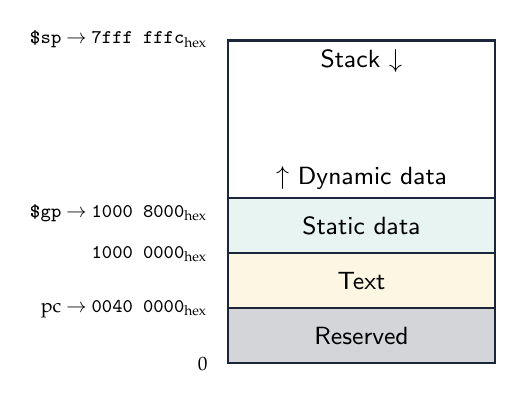
\begin{tikzpicture}[s/.style={draw=ink,thick,minimum width=34mm,font=\small\sffamily}]
\node[s,minimum height=20mm,fill=white,anchor=south] (st) at (0,27mm) {};
\node[font=\small\sffamily,anchor=north] at (st.north) {Stack $\downarrow$};
\node[font=\small\sffamily,anchor=south] at (st.south) {$\uparrow$ Dynamic data};
\node[s,minimum height=7mm,fill=mist,anchor=south] (sd) at (0,20mm) {Static data};
\node[s,minimum height=7mm,fill=goldbg,anchor=south] (tx) at (0,13mm) {Text};
\node[s,minimum height=7mm,fill=slate!30,anchor=south] (rs) at (0,6mm) {Reserved};
\node[tk,anchor=east] at ([xshift=-2mm]st.north west) {\reg{sp} $\to$ \texttt{7fff fffc}$_{\text{hex}}$};
\node[tk,anchor=east] at ([xshift=-2mm,yshift=-2mm]sd.north west) {\reg{gp} $\to$ \texttt{1000 8000}$_{\text{hex}}$};
\node[tk,anchor=east] at ([xshift=-2mm]sd.south west) {\texttt{1000 0000}$_{\text{hex}}$};
\node[tk,anchor=east] at ([xshift=-2mm]tx.south west) {pc $\to$ \texttt{0040 0000}$_{\text{hex}}$};
\node[tk,anchor=east] at ([xshift=-2mm]rs.south west) {0};
\end{tikzpicture}}
\begin{center}\small Figure for Question 5(c)-3: The MIPS memory allocation for program and data.\end{center}
\end{question}
\begin{solution}
\sub{What the linker does (slides: ``Linking Object Modules'')}
(1) \textbf{merge} the text segments and the data segments, (2) \textbf{resolve} every label to an absolute address, (3) \textbf{patch} each location listed in the relocation information.

\sub{Step 1: place the segments (Figure 5(c)-3)}
\begin{itemize}
  \item Text starts at \hex{00400000}. Procedure A's text (\hex{150} bytes) occupies \hex{00400000}--\hex{0040014C}. Procedure B's text (\hex{350} bytes) follows at \hex{00400150}--\hex{0040049C}.
  \item Static data starts at \hex{10000000}. A's data (\hex{40} bytes) is at \hex{10000000}--\hex{1000003C}, and B's data (\hex{50} bytes) follows at \hex{10000040}--\hex{1000008C}.
\end{itemize}
\sub{Step 2: resolve the symbols}
\fig{\small\begin{tabular}{llll}\toprule
Label & Belongs to & Address & Used by\\\midrule
A & start of A's text & \hex{00400000} & \ins{jal} in B\\
B & start of B's text & \hex{00400000}$+$\hex{150} $=$ \hex{00400150} & \ins{jal} in A\\
X & A's data word 0 & \hex{10000000} & \ins{lw} in A\\
Y & B's data word 0 & \hex{10000000}$+$\hex{40} $=$ \hex{10000040} & \ins{sw} in B\\\bottomrule
\end{tabular}}
\sub{Step 3: patch the relocated instructions}
\begin{itemize}
  \item \ins{lw}/\ins{sw} use base addressing off \reg{gp}$\,=\,$\hex{10008000}, so the 16-bit offset is (address $-$ \reg{gp}):\\
  X: \hex{10000000}$-$\hex{10008000} $=-$\hex{8000} $=-32768$, so the field is \hex{8000}.\\
  Y: \hex{10000040}$-$\hex{10008000} $=-$\hex{7FC0} $=-32704$, so the field is \hex{8040}.
  \item \ins{jal} uses pseudodirect addressing, so its 26-bit field is (target $\div 4$):\\
  \ins{jal B}: \hex{00400150}$/4=$ \hex{0100054}. \ins{jal A}: \hex{00400000}$/4=$ \hex{0100000}. Both lie in the same 256\,MB region as the calls (upper 4 bits 0000).
\end{itemize}
\sub{The executable file}
\fig{\small\begin{tabular}{l|l|l}\toprule
\multicolumn{3}{l}{\textbf{Executable file header}: Text size \hex{4A0} ($=$\hex{150}$+$\hex{350}), Data size \hex{90} ($=$\hex{40}$+$\hex{50})}\\\midrule
Text segment & \textbf{Address} & \textbf{Instruction}\\
 & \hex{00400000} & \ins{lw \$a0, 8000}$_{\text{hex}}$\ins{(\$gp)}\quad\textit{(i.e.\ $-32768$(\$gp) $\to$ X)}\\
 & \hex{00400004} & \ins{jal 400150}$_{\text{hex}}$\quad\textit{(field \hex{0100054})}\\
 & \ldots & \ldots\\
 & \hex{00400150} & \ins{sw \$a1, 8040}$_{\text{hex}}$\ins{(\$gp)}\quad\textit{(i.e.\ $-32704$(\$gp) $\to$ Y)}\\
 & \hex{00400154} & \ins{jal 400000}$_{\text{hex}}$\quad\textit{(field \hex{0100000})}\\
 & \ldots & \ldots\\\midrule
Data segment & \hex{10000000} & (X)\\
 & \ldots & \ldots\\
 & \hex{10000040} & (Y)\\
 & \ldots & \ldots\\\bottomrule
\end{tabular}}
\ans{A's text is at \hex{00400000} and B's at \hex{00400150}; X is at \hex{10000000} and Y at \hex{10000040}. The patched instructions are: \hex{00400000}: \ins{lw \$a0,0x8000(\$gp)}; \hex{00400004}: \ins{jal 0x00400150}; \hex{00400150}: \ins{sw \$a1,0x8040(\$gp)}; \hex{00400154}: \ins{jal 0x00400000}. The executable has text size \hex{4A0} and data size \hex{90}.}
\end{solution}

%---------------------------------------------------------------- IS11
\repeated{5}
\begin{question}{2022--2023 \textbullet\ Q6(b)}{CSE 305 \textbullet\ 25/04/2024 \textbullet\ IS11}{7}
What support does the MIPS instruction-set architecture provide for synchronization? Explain with an example.
\end{question}
\begin{question}{2016--2017 \textbullet\ Q6(b)}{CSE 305 \textbullet\ 02/08/2017 \textbullet\ IS11}{10}
What support does MIPS instruction set architecture provide for synchronization? Explain with an example.
\end{question}
\begin{question}{2015--2016 \textbullet\ Q6(c)}{CSE 305 \textbullet\ 18/01/2017 \textbullet\ IS11}{8}
What is data race? What instructions are available in MIPS to address this issue? How these instructions work?
\end{question}
\begin{question}{2014--2015 \textbullet\ Q6(b)}{CSE 305 \textbullet\ 26/01/2016 \textbullet\ IS11}{5}
What support does MIPS instruction set architecture provide for synchronization?
\end{question}
\begin{question}{2013--2014 \textbullet\ Q7(a)}{CSE 305 \textbullet\ 05/07/2015 \textbullet\ IS11}{8}
Briefly describe the two instructions used for synchronization in MIPS. Write down the MIPS code to do the following atomically:
\[\texttt{A[0] = X}\]
Consider the base address of A is in \reg{s1} and X is in \reg{s2}.
\end{question}
\begin{solution}
\sub{Data race and why hardware support is needed}
Two processors (or threads) share a memory location, and P1 writes it while P2 reads or writes it. If they do not synchronize, the result depends on the \emph{order of the accesses}. This is a \key{data race}. Example: both execute \texttt{count = count + 1} as \ins{lw}/\ins{addi}/\ins{sw}. If both \ins{lw} instructions happen before either \ins{sw}, one increment is lost. Locks need an \textbf{atomic read-modify-write}: no other access to the location may come between the read and the write. Hardware can provide this as one instruction (e.g.\ atomic swap) or as an \textbf{atomic pair of instructions}, which is what MIPS does.

\sub{MIPS support: \ins{ll} / \ins{sc}}
\begin{itemize}
  \item \ins{ll rt, offset(rs)}, \key{load linked}: loads the word like \ins{lw} and remembers (\emph{links}) its address in the hardware.
  \item \ins{sc rt, offset(rs)}, \key{store conditional}: stores rt to that address \emph{only if the location has not been changed since the matching} \ins{ll}. On success it writes \textbf{1} into rt; on failure (another store to the location, or a context switch) it does not store and writes \textbf{0} into rt.
  \item Software loops back and retries when \ins{sc} returns 0, so the \ins{ll}--\ins{sc} pair behaves as one atomic operation without locking the memory bus.
\end{itemize}

\sub{Example: atomic swap of \reg{s4} with Mem[\reg{s1}] (slides), used to build a lock}
\begin{mips}
try: add  $t0, $zero, $s4   # copy exchange value
     ll   $t1, 0($s1)       # load linked:   $t1 = Mem[$s1]
     sc   $t0, 0($s1)       # store conditional: Mem[$s1] = $t0 if unchanged
     beq  $t0, $zero, try   # sc failed (0) -> retry
     add  $s4, $zero, $t1   # put loaded (old) value in $s4
\end{mips}
With \reg{s4}$=1$ this is a \emph{test-and-set}. If the old value returned is 0, the lock was free and is now ours. If it is 1, someone else holds it, so spin and try again. The lock is released by an ordinary \ins{sw \$zero,0(\$s1)}.
\fig{\small\setlength{\tabcolsep}{5pt}\begin{tabular}{cll}\toprule
time & P1 & P2\\\midrule
1 & \ins{ll \$t1,0(\$s1)} (reads 0) & \\
2 & & \ins{ll \$t1,0(\$s1)} (reads 0)\\
3 & & \ins{sc \$t0,0(\$s1)} $\to$ \reg{t0}$=1$, lock acquired\\
4 & \ins{sc \$t0,0(\$s1)} $\to$ \reg{t0}$=0$ (location changed) & \\
5 & \ins{beq} $\to$ retry, now reads 1: busy & \\\bottomrule
\end{tabular}}

\sub{2013--2014 card: \texttt{A[0] = X} atomically (\&A[0] in \reg{s1}, X in \reg{s2})}
\begin{mips}
try: add  $t0, $zero, $s2   # $t0 = X (sc overwrites its register)
     ll   $t1, 0($s1)       # load-link A[0] (old value)
     sc   $t0, 0($s1)       # A[0] = X only if no one wrote A[0] since ll
     beq  $t0, $zero, try   # failed -> repeat
\end{mips}
After the loop, A[0] $=$ X has been written atomically, and the old A[0] is in \reg{t1} if it is needed.
\ans{MIPS provides the atomic pair \ins{ll} (load linked) and \ins{sc} (store conditional). \ins{sc} succeeds and returns 1 only if the location was not modified since the \ins{ll}; otherwise it returns 0 and the code retries. Together they implement atomic swap and locks, which prevent data races.}
\end{solution}

%---------------------------------------------------------------- IS12
\begin{question}{2022--2023 \textbullet\ Q6(c)}{CSE 305 \textbullet\ 25/04/2024 \textbullet\ IS12}{8}
Write down the equivalent MIPS code for the following C code, considering registers \reg{t1} and \reg{t2} for variables \ins{x} and \ins{y}, respectively:
\begin{ccode}
if (x > y + 131075)
    x = 8;
\end{ccode}
\end{question}
\begin{solution}
\sub{Key points}
\begin{itemize}
  \item I-format immediates are 16-bit signed ($-32768\ldots32767$). $131075 = 2\times65536+3 =$ \hex{00020003} does not fit, so it is built with \ins{lui} (upper half 2) and \ins{ori} (lower half 3).
  \item MIPS has no ``branch if greater''. Rewrite $x > y+131075$ as $(y+131075) < x$ and use \ins{slt} followed by \ins{beq} against \reg{zero}.
\end{itemize}
\begin{mips}
      lui  $t0, 2             # $t0 = 2 << 16 = 131072
      ori  $t0, $t0, 3        # $t0 = 131075
      add  $t0, $t2, $t0      # $t0 = y + 131075
      slt  $t3, $t0, $t1      # $t3 = 1 if (y+131075) < x
      beq  $t3, $zero, Exit   # condition false -> skip
      addi $t1, $zero, 8      # x = 8
Exit:
\end{mips}
\ans{Build 131075 with \ins{lui \$t0,2}; \ins{ori \$t0,\$t0,3}. Then \ins{add \$t0,\$t2,\$t0}; \ins{slt \$t3,\$t0,\$t1}; \ins{beq \$t3,\$zero,Exit}; \ins{addi \$t1,\$zero,8}; \ins{Exit:}.}
\end{solution}

%---------------------------------------------------------------- IS13
\begin{question}{2022--2023 \textbullet\ Q7(b)}{CSE 305 \textbullet\ 25/04/2024 \textbullet\ IS13}{7}
Chandler has used 40 variables in his program, whereas the MIPS architecture has only 32 registers. What does the compiler do in such a scenario?
\end{question}
\begin{solution}
The compiler performs \key{register allocation} and \key{spilling} (slides: ``Registers vs.\ Memory'': \emph{only spill to memory for less frequently used variables}).
\begin{itemize}
  \item Not all 32 registers are free for variables: \reg{zero}, \reg{at}, \reg{k0}/\reg{k1}, \reg{gp}, \reg{sp}, \reg{fp} and \reg{ra} are reserved. About 24 (\reg{s0}--\reg{s7}, \reg{t0}--\reg{t9}, \reg{a0}--\reg{a3}, \reg{v0}/\reg{v1}) can hold values.
  \item \textbf{Live-range analysis:} a register is needed only while a variable is \emph{live}, i.e.\ between its assignment and its last use. Variables whose live ranges do not overlap can share one register (graph-colouring allocation). So 40 variables often need far fewer than 40 registers at any one moment.
  \item \textbf{Spilling:} when more values are live than there are registers, the compiler keeps the most frequently used ones (e.g.\ loop counters, values in inner loops) in registers. The rest live in memory, normally in the procedure's stack frame. Before a spilled variable is used it is loaded with \ins{lw}; after it is changed it is stored back with \ins{sw}:
\begin{mips}
lw   $t0, 24($sp)     # bring spilled variable v into a register
addi $t0, $t0, 1      # v = v + 1
sw   $t0, 24($sp)     # spill it back to the stack frame
\end{mips}
  \item Callee-saved \reg{s} registers that it reuses are themselves saved and restored on the stack.
\end{itemize}
Spilled variables cost extra instructions and slower memory accesses, so good allocation (``register optimization is important'') directly improves performance.
\ans{The compiler allocates registers to the most frequently used, simultaneously live variables (reusing registers when live ranges do not overlap) and \emph{spills} the rest to memory, the stack frame, accessing them with \ins{lw}/\ins{sw} when needed.}
\end{solution}

%---------------------------------------------------------------- IS14
\begin{question}{2022--2023 \textbullet\ Q7(c)}{CSE 305 \textbullet\ 25/04/2024 \textbullet\ IS14}{8}
Translate function \ins{f} (defined below) into MIPS assembly language. If you need to use registers \reg{t0} through \reg{t7}, use the lower-numbered registers first. Assume the function declaration for \ins{func} is ``\ins{int func(int a, int b);}''. The code for function \ins{f} is as follows:
\begin{ccode}
int f (int a, int b, int c, int d) {
    return func(func(a,b), c+d);
}
\end{ccode}
\end{question}
\begin{solution}
\sub{Analysis}
\begin{itemize}
  \item By convention \ins{a}, \ins{b}, \ins{c}, \ins{d} arrive in \reg{a0}--\reg{a3}, and results come back in \reg{v0}.
  \item \ins{f} is \textbf{non-leaf}: it calls \ins{func} twice, so it must save \reg{ra}.
  \item \ins{c+d} is needed \emph{after} the first call, but \reg{a2}, \reg{a3} and \reg{t0}--\reg{t9} may be destroyed by \ins{func} (caller-saved). So we compute \ins{c+d} into \reg{t0} (lowest temporary first) and save it on the stack across the call.
  \item The first call needs \ins{(a,b)}, which are already in \reg{a0}, \reg{a1}. The second call needs \reg{a0}$=$\ins{func(a,b)} and \reg{a1}$=$\ins{c+d}.
\end{itemize}
\fig{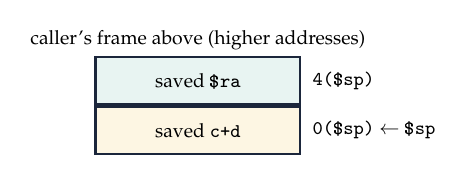
\begin{tikzpicture}[c/.style={draw=ink,thick,minimum width=26mm,minimum height=6mm,font=\scriptsize}]
\node[c,fill=mist] (r) {saved \reg{ra}};
\node[c,fill=goldbg,below=0pt of r] (s) {saved \ins{c+d}};
\node[tk,right=1mm of r] {\ins{4(\$sp)}};
\node[tk,right=1mm of s] {\ins{0(\$sp)} $\leftarrow$ \reg{sp}};
\node[tk,above=1pt of r] {caller's frame above (higher addresses)};
\end{tikzpicture}}
\begin{mips}
f:   addi $sp, $sp, -8      # make room for 2 words
     sw   $ra, 4($sp)       # save return address
     add  $t0, $a2, $a3     # $t0 = c + d
     sw   $t0, 0($sp)       # save c+d ($t0 is not preserved by func)
     jal  func              # $v0 = func(a, b)   (a,b already in $a0,$a1)
     add  $a0, $v0, $zero   # 1st argument = func(a, b)
     lw   $a1, 0($sp)       # 2nd argument = c + d
     jal  func              # $v0 = func(func(a,b), c+d)
     lw   $ra, 4($sp)       # restore return address
     addi $sp, $sp, 8       # pop the frame
     jr   $ra               # return; result already in $v0
\end{mips}
\begin{note}Optimisation (not required): the second call is a tail call. One can restore \reg{ra}, pop the frame, and then end with \ins{j func} instead of \ins{jal func} \ldots\ \ins{jr \$ra}. This saves one instruction.\end{note}
\ans{The 11-instruction procedure above. It uses a 2-word stack frame holding \reg{ra} and \ins{c+d} (computed in \reg{t0}). The first \ins{jal func} uses \reg{a0}, \reg{a1} as given. Then \reg{a0}$\leftarrow$\reg{v0} and \reg{a1}$\leftarrow$\ins{c+d}, followed by the second \ins{jal func}. The result is returned in \reg{v0}.}
\end{solution}

%---------------------------------------------------------------- IS15
\repeated{5}
\begin{question}{2021--2022 \textbullet\ Q5(a)}{CSE 305 \textbullet\ 06/04/2023 \textbullet\ IS15}{3$\times$5 = 15}
The following four design principles have been guiding the instruction-set designers to find a balance between the number of instructions needed to execute a program, the number of clock cycles needed by an instruction, and the speed of the clock.
\begin{enumerate}
  \item Simplicity favors regularity
  \item Smaller is faster
  \item Good design demands good compromise
  \item[\textbf{(vi)}] Make the common case faster
\end{enumerate}
You are given several design features of MIPS instruction-set architecture in the following. Now, please identify which of the above principle(s) is behind each of these design decisions.
\begin{enumerate}
  \item Keeping conditional branch's offset value in a range of 16 bits.
  \item Keeping 32 registers rather than many more.
  \item Consistent instruction format, i.e., always requiring three registers for R-type Instructions.
  \item Multiple instruction formats to allow flexibility.
  \item Reduced instruction set, Complex instructions (i.e., pseudo instructions like \ins{bgt}, \ins{bge}, \ins{mov} etc.) are translated into one or more basic instructions.
\end{enumerate}
\end{question}
\begin{question}{2020--2021 \textbullet\ Q11(d)}{CSE 305 \textbullet\ 24/09/2022 \textbullet\ IS15}{5}
Provide an illustrative example for showing how MIPS architecture follows the design principle: ``Good design demands good compromises.''
\end{question}
\begin{question}{2016--2017 \textbullet\ Q6(c)}{CSE 305 \textbullet\ 02/08/2017 \textbullet\ IS15}{15}
The following four design principles have been guiding the instruction-set designers to find a balance between the number of instructions needed to execute a program, the number of clock cycles needed by an instruction, and the speed of the clock.
\begin{enumerate}
  \item Simplicity favors regularity
  \item Smaller is faster
  \item Good design demands good compromise
  \item Make the common case faster
\end{enumerate}
- You are given several design features of MIPS instruction-set architecture in the following. Now, please identify that which of the above principles are behind these design decisions.
\begin{enumerate}
  \item keeping instruction immediate value in a range of 16-bits
  \item always requiring three register operands in arithmetic instructions
  \item using PC-relative addressing for conditional branching
  \item keeping 32 registers rather than many more
  \item keeping the register fields in the same place in each instruction format
\end{enumerate}
\end{question}
\begin{question}{2013--2014 \textbullet\ Q6(a)}{CSE 305 \textbullet\ 05/07/2015 \textbullet\ IS15}{8}
What are the four design principles used for MIPS instruction set design? What are the steps for starting a Java application?
\end{question}
\begin{question}{2011--2012 \textbullet\ Q2(a)}{CSE 305 \textbullet\ 27/07/2013 \textbullet\ IS15}{4 + 4}
What are the MIPS design principles? Mention one use of each of these design principles in MIPS ISA.
\end{question}
\begin{solution}
\sub{The four design principles, with one use of each (2013--14, 2011--12)}
{\small\begin{tabularx}{\linewidth}{@{}>{\raggedright\arraybackslash}p{40mm}>{\raggedright\arraybackslash}X@{}}
\toprule
Principle & Use in MIPS\\
\midrule
1. Simplicity favours regularity & Every arithmetic instruction has exactly 3 register operands (\ins{add a,b,c}). All instructions are 32 bits, and fields keep the same positions across formats. Regular hardware is simpler and faster.\\
2. Smaller is faster & Only 32 registers. A small register file has short wires and fast access, and 5-bit register fields keep instructions short.\\
3. Make the common case fast & Small constants are common, so there are immediate instructions (\ins{addi \$s3,\$s3,4}) that avoid a load. \reg{zero} makes moves cheap. Branches use PC-relative addressing because most targets are near.\\
4. Good design demands good compromises & Three formats (R, I, J) instead of one: decoding is a little more complex, but every instruction stays 32 bits. As a result immediates and branch offsets are limited to 16 bits.\\
\bottomrule
\end{tabularx}}

\sub{2021--2022 Q5(a)}
The paper numbers the fourth principle ``(vi)'', a misprint for (iv). The numbering below keeps the paper's labels.\par
{\small\begin{tabularx}{\linewidth}{@{}>{\raggedright\arraybackslash}p{40mm}>{\raggedright\arraybackslash}p{36mm}>{\raggedright\arraybackslash}X@{}}
\toprule
Decision & Principle & Reason\\
\midrule
(i) 16-bit branch offset & (iii) Good compromise (also (vi)) & Keeps a fixed 32-bit I-format with op, rs, rt. 16 bits suffice for the common near branches. Far targets use \ins{bne}$+$\ins{j}.\\
(ii) 32 registers & (ii) Smaller is faster & More registers mean a slower register file, longer clock and more field bits.\\
(iii) Always 3 registers in R-type & (i) Simplicity favours regularity & One uniform form makes decoding and the datapath simple.\\
(iv) Multiple formats & (iii) Good compromise & Different needs (registers, constants, long jump addresses) are met while the length stays at 32 bits and formats stay similar.\\
(v) Reduced set; pseudo-instructions & (vi) Common case fast (also (i)) & Hardware implements only simple, frequent operations, so they run fast. Rare ``complex'' ones (\ins{bgt}, \ins{bge}, \ins{move}) are synthesized by the assembler (\ins{slt}$+$\ins{bne}, \ins{add \$t0,\$zero,\$t1}).\\
\bottomrule
\end{tabularx}}

\sub{2016--2017 Q6(c)}
{\small\begin{tabularx}{\linewidth}{@{}>{\raggedright\arraybackslash}p{40mm}>{\raggedright\arraybackslash}p{36mm}>{\raggedright\arraybackslash}X@{}}
\toprule
Decision & Principle & Reason\\
\midrule
(i) 16-bit immediates & (iii) Good compromise (also (iv)) & Fits the fixed 32-bit format. Most constants are small, and \ins{lui}$+$\ins{ori} handle the rest.\\
(ii) 3 register operands in arithmetic & (i) Simplicity favours regularity & Same form for all arithmetic instructions.\\
(iii) PC-relative conditional branches & (iv) Make the common case fast & Most branch targets are near (loops, ifs), so a 16-bit relative offset is enough.\\
(iv) 32 registers & (ii) Smaller is faster & A larger register file would be slower.\\
(v) Register fields in the same place in every format & (i) Simplicity favours regularity (also (iii)) & Registers can be read before the opcode is decoded, and the hardware is simpler.\\
\bottomrule
\end{tabularx}}

\sub{2020--2021 Q11(d): an illustration of ``good design demands good compromises''}
MIPS wants \emph{all instructions the same length (32 bits)} for simple fetch and decode, and \emph{large constants and addresses} for convenience. These goals conflict, and the compromise is to use \textbf{several formats while keeping them as similar as possible}:
\fig{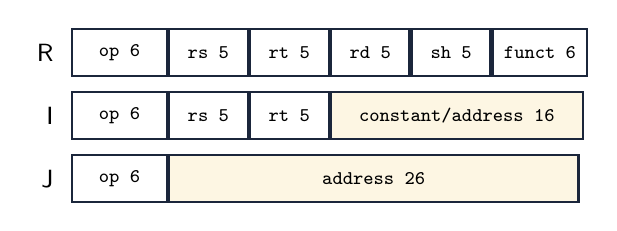
\begin{tikzpicture}[f/.style={draw=ink,thick,minimum height=6mm,font=\scriptsize\ttfamily,inner sep=1pt}]
\foreach \y/\t in {0/R,-8/I,-16/J}{\node[anchor=east,font=\small\sffamily] at (-1mm,\y mm) {\t};}
\node[f,minimum width=12mm,anchor=west] (r1) at (0,0) {op 6}; \node[f,minimum width=10mm,right=0pt of r1] (r2) {rs 5};
\node[f,minimum width=10mm,right=0pt of r2] (r3) {rt 5}; \node[f,minimum width=10mm,right=0pt of r3] (r4) {rd 5};
\node[f,minimum width=10mm,right=0pt of r4] (r5) {sh 5}; \node[f,minimum width=12mm,right=0pt of r5] {funct 6};
\node[f,minimum width=12mm,anchor=west] (i1) at (0,-8mm) {op 6}; \node[f,minimum width=10mm,right=0pt of i1] (i2) {rs 5};
\node[f,minimum width=10mm,right=0pt of i2] (i3) {rt 5}; \node[f,fill=goldbg,minimum width=32mm,right=0pt of i3] {constant/address 16};
\node[f,minimum width=12mm,anchor=west] (j1) at (0,-16mm) {op 6}; \node[f,fill=goldbg,minimum width=52mm,right=0pt of j1] {address 26};
\end{tikzpicture}}
op, rs and rt stay in the same positions, so decoding stays simple. The price is that I-format immediates and branch offsets are only 16 bits, which is why \ins{lui} is needed for 32-bit constants and \ins{bne}$+$\ins{j} for far branches. A second example is not providing \ins{blt}/\ins{bge}: a combined compare-and-branch would slow the clock for every instruction, so MIPS uses \ins{slt}$+$\ins{beq}/\ins{bne}.

\sub{Steps for starting a Java application (2013--14)}
\begin{enumerate}
  \item The Java compiler translates the Java program into \textbf{class files of Java bytecodes}, a simple, portable instruction set for the JVM.
  \item The \textbf{Java Virtual Machine} loads the class files, together with the Java library routines, which are also bytecodes.
  \item The JVM \textbf{interprets} the bytecodes, which gives portability.
  \item A \textbf{JIT compiler} profiles the program and compiles the bytecodes of ``hot'' methods into \textbf{native machine code} for the host, which is then executed directly and reused (slides: ``Starting Java Applications'').
\end{enumerate}
\ans{The four principles are simplicity favours regularity, smaller is faster, make the common case fast, and good design demands good compromises. 2021--22: (i) compromise, (ii) smaller is faster, (iii) regularity, (iv) compromise, (v) common case fast. 2016--17: (i) compromise, (ii) regularity, (iii) common case fast, (iv) smaller is faster, (v) regularity.}
\end{solution}

%---------------------------------------------------------------- IS16
\begin{question}{2021--2022 \textbullet\ Q6(a)}{CSE 305 \textbullet\ 06/04/2023 \textbullet\ IS16}{15}
Write the MIPS assembly code for the C code shown in the following figure (Figure: 6.a).
\begin{ccode}
int fib(int n) {
    if (n==0) return 0;
    else if (n == 1) return 1;
    else return fib(n-1) + fib(n-2);
}
\end{ccode}
\centerline{\small Figure: 6.a}
\end{question}
\begin{solution}
\textbf{Conventions} (slides): argument \reg{a0} $=n$, result in \reg{v0}, return address \reg{ra}.
\texttt{fib} is a \key{non-leaf} procedure that calls itself \emph{twice}, so across the calls it must keep
\reg{ra}, the original $n$ (needed to form $n-2$) and the value of \texttt{fib(n-1)} (needed for the final add).
We keep \texttt{fib(n-1)} in the callee-saved register \reg{s0}, so \reg{s0} itself must also be saved.
Both base cases return $n$ itself ($0\to0$, $1\to1$), so they share one exit.

\begin{mips}
fib:    beq  $a0, $zero, Base     # n == 0 ?
        addi $t0, $zero, 1
        beq  $a0, $t0, Base       # n == 1 ?
        addi $sp, $sp, -12        # make room for 3 words
        sw   $ra, 8($sp)          # save return address
        sw   $a0, 4($sp)          # save n
        sw   $s0, 0($sp)          # save caller's $s0
        addi $a0, $a0, -1         # argument n-1
        jal  fib                  # $v0 = fib(n-1)
        add  $s0, $v0, $zero      # keep fib(n-1) in $s0
        lw   $a0, 4($sp)          # restore n
        addi $a0, $a0, -2         # argument n-2
        jal  fib                  # $v0 = fib(n-2)
        add  $v0, $s0, $v0        # fib(n-1) + fib(n-2)
        lw   $s0, 0($sp)          # restore $s0
        lw   $ra, 8($sp)          # restore return address
        addi $sp, $sp, 12         # pop the frame
        jr   $ra                  # return
Base:   add  $v0, $a0, $zero      # return 0 or 1 (= n)
        jr   $ra
\end{mips}

\fig{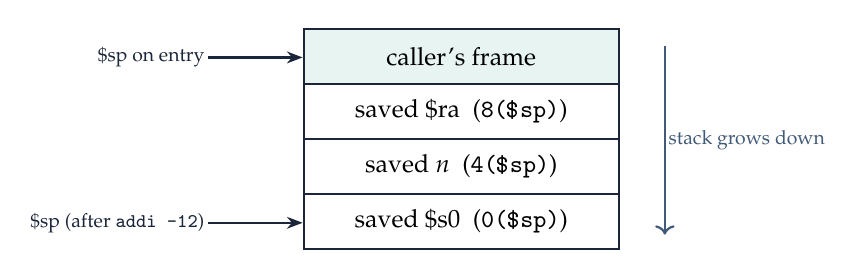
\begin{tikzpicture}[x=1mm,y=1mm,font=\small]
  \foreach \y/\t in {0/{saved \$s0 \ (\texttt{0(\$sp)})},7/{saved $n$ \ (\texttt{4(\$sp)})},14/{saved \$ra \ (\texttt{8(\$sp)})}}
    \node[blk,minimum width=40mm,minimum height=7mm,anchor=south west] at (0,\y) {\t};
  \node[blk,fill=mist,minimum width=40mm,minimum height=7mm,anchor=south west] at (0,21) {caller's frame};
  \draw[wire] (-12,3.5) node[left,tk]{\$sp (after \texttt{addi -12})} -- (0,3.5);
  \draw[wire] (-12,24.5) node[left,tk]{\$sp on entry} -- (0,24.5);
  \draw[->,thick,inksoft] (46,26) -- node[right,tk]{stack grows down} (46,2);
\end{tikzpicture}}
The base cases are tested exactly as in the C code ($n=0$, $n=1$). Each call that does not hit a base case
pushes a 3-word frame and pops it before \ins{jr \$ra}, so every caller finds \reg{sp}, \reg{s0} and \reg{ra} as it left them.
\end{solution}

%---------------------------------------------------------------- IS17
\begin{question}{2021--2022 \textbullet\ Q6(b)}{CSE 305 \textbullet\ 06/04/2023 \textbullet\ IS17}{5 + 5}
Suppose the program counter (PC) is set to \texttt{0x2000 0000}. Explain your answer for the following questions.
\begin{enumerate}
  \item Is it possible to use the jump (\ins{j}) MIPS assembly instruction to set the PC to the address \texttt{0x4000 0000}?
  \item Is it possible to use single branch (\ins{beq}/\ins{bneq}) instruction to set the PC to this same address?
\end{enumerate}
\end{question}
\begin{solution}
\sub{Facts used}
\begin{itemize}
  \item \ins{j} (pseudodirect, J-format): target $=$ (PC$+4$)$_{31..28}$ : addr$_{26}$ : 00. Only the low 28 bits come from the instruction; the upper 4 bits are copied from PC$+4$.
  \item \ins{beq}/\ins{bne} (PC-relative, I-format): target $=$ PC$+4+$SignExt(off$_{16}$)$\times4$. The reach is $-2^{17}\ldots+2^{17}-4$ bytes ($\approx\pm128$\,KB).
\end{itemize}
\textbf{(i)} PC$+4=$ \hex{20000004}, upper 4 bits \texttt{0010}. The target \hex{40000000} has upper 4 bits \texttt{0100}. These differ, so \ins{j} \textbf{cannot} reach it: the target is in another 256\,MB region.\\
\textbf{(ii)} The required distance is \hex{40000000}$-$\hex{20000004} $=$ \hex{1FFFFFFC} $=536{,}870{,}908$ bytes, i.e.\ $\approx1.3\times10^8$ words. That is far beyond the 16-bit offset limit of $32767$ words. So \textbf{no}.\\
\textbf{How to do it:} load the full address into a register and use \ins{jr}:
\begin{mips}
lui  $t0, 0x4000          # $t0 = 0x4000 0000
jr   $t0                  # PC = 0x4000 0000
\end{mips}
\ans{(i) No: \ins{j} keeps PC$_{31..28}=$\,0010, but the target needs 0100. (ii) No: the distance \hex{1FFFFFFC} bytes far exceeds the $\pm2^{17}$-byte branch range. Use \ins{lui \$t0,0x4000}; \ins{jr \$t0}.}
\end{solution}

%---------------------------------------------------------------- IS18
\begin{question}{2020--2021 \textbullet\ Q11(c)}{CSE 305 \textbullet\ 24/09/2022 \textbullet\ IS18}{12}
Write the equivalent efficient sequence of MIPS instructions for the following C code fragment.
\begin{ccode}
int testFunc (int a, int b, int c)
{
    int i=0, result=0;
    do
    {
        if(i>b)
            result += c;
        i++;
    } while (i<a);
    return result;
}
\end{ccode}
Assume, \reg{s1} and \reg{s2} will carry the values of variable \emph{i} and variable \emph{result}, respectively.
\end{question}
\begin{solution}
\textbf{Register use:} $a,b,c$ arrive in \reg{a0}, \reg{a1}, \reg{a2} (argument registers); $i=$ \reg{s1},
$result=$ \reg{s2}; the return value goes in \reg{v0}. Because \reg{s1}, \reg{s2} are \key{callee-saved}, the
procedure saves/restores them on the stack.

\textbf{Efficiency points:} a \texttt{do-while} loop needs \emph{no} test at the top --- the body runs once and the
loop-closing branch is at the bottom (one branch per iteration). MIPS has no \ins{bgt}/\ins{blt}, so
$i>b \Leftrightarrow b<i$ is computed with \ins{slt} and combined with \ins{beq}/\ins{bne} against \reg{zero}.

\begin{mips}
testFunc: addi $sp, $sp, -8       # save callee-saved registers
          sw   $s1, 4($sp)
          sw   $s2, 0($sp)
          add  $s1, $zero, $zero  # i = 0
          add  $s2, $zero, $zero  # result = 0
Loop:     slt  $t0, $a1, $s1      # $t0 = (b < i)  i.e. (i > b)
          beq  $t0, $zero, Skip   # if !(i > b) skip the add
          add  $s2, $s2, $a2      # result += c
Skip:     addi $s1, $s1, 1        # i++
          slt  $t0, $s1, $a0      # $t0 = (i < a)
          bne  $t0, $zero, Loop   # repeat while (i < a)
          add  $v0, $s2, $zero    # return result
          lw   $s2, 0($sp)        # restore $s2, $s1
          lw   $s1, 4($sp)
          addi $sp, $sp, 8
          jr   $ra
\end{mips}
The loop body is only 6 instructions (5 when the \texttt{if} is false). If the caller does not need \reg{s1},
\reg{s2} preserved, the 6 save/restore instructions can be dropped.
\end{solution}

%---------------------------------------------------------------- IS19
\begin{question}{2020--2021 \textbullet\ Q12(b)}{CSE 305 \textbullet\ 24/09/2022 \textbullet\ IS19}{10}
Consider the following MIPS code:
\begin{mips}
L1: bne $t0, $t1, L3
L2: j LX
L3: addi $t0, $t1, 1
\end{mips}
Now, if the opcode of \emph{j}, \emph{bne} and \emph{addi} are 2, 5 and 8 respectively, the register \reg{t0} and
\reg{t1} are indicated by register values 8 and 9 respectively, and the addresses are
\begin{center}L1 $\to$ 1000, \qquad L2 $\to$ 1004, \qquad L3 $\to$ 1008, \qquad LX $\to$ 131072,\end{center}
then, write down the instruction format name and the instruction values for each of the above-mentioned
instructions. The following example is provided as a hint.

\textbf{Example:} Consider the following MIPS instruction: \ins{add \$s1, \$s2, \$s3}.
The instruction format is R-format and instruction values should be:
\fig{\begin{tabular}{r|c|c|c|c|c|c|}
\cline{2-7}
Address & 6 bits & 5 bits & 5 bits & 5 bits & 5 bits & 6 bits\\ \cline{2-7}
0400 & 0 & 18 & 19 & 17 & 0 & 0\\ \cline{2-7}
\end{tabular}}
\end{question}
\begin{solution}
\sub{Method}
\fig{{\small\setlength{\tabcolsep}{0pt}%
\begin{tabular}{r|*{6}{>{\centering\arraybackslash}p{15mm}|}}
\cline{2-7}
\textbf{R}\ \ & op (6) & rs (5) & rt (5) & rd (5) & shamt (5) & funct (6)\\ \cline{2-7}
\multicolumn{7}{c}{}\\[-8pt] \cline{2-7}
\textbf{I}\ \ & op (6) & rs (5) & rt (5) & \multicolumn{3}{c|}{constant / offset (16)}\\ \cline{2-7}
\multicolumn{7}{c}{}\\[-8pt] \cline{2-7}
\textbf{J}\ \ & op (6) & \multicolumn{5}{c|}{address (26)}\\ \cline{2-7}
\end{tabular}}}
\begin{itemize}
\item \ins{bne rs, rt, L} and \ins{addi rt, rs, imm} are \key{I-format}; \ins{j} is \key{J-format}.
\item Branch (PC-relative): $\text{offset} = \dfrac{\text{target} - (\text{PC}_{\text{branch}}+4)}{4}$ words.
  Jump (pseudo-direct): $\text{field} = \dfrac{\text{target}}{4}$; the upper 4 bits of the target come from PC+4.
\end{itemize}
\sub{Encoding}
\fig{{\small\setlength{\tabcolsep}{4pt}%
\begin{tabular}{r l l|c|c|c|c|c|c|}
\cline{4-9}
Addr & Instruction & Format & 6 bits & 5 bits & 5 bits & 5 bits & 5 bits & 6 bits\\ \cline{4-9}
1000 & \ins{bne \$t0,\$t1,L3} & I-format & 5 & 8 & 9 & \multicolumn{3}{c|}{1}\\ \cline{4-9}
1004 & \ins{j LX} & J-format & 2 & \multicolumn{5}{c|}{32768}\\ \cline{4-9}
1008 & \ins{addi \$t0,\$t1,1} & I-format & 8 & 9 & 8 & \multicolumn{3}{c|}{1}\\ \cline{4-9}
\end{tabular}}}
\begin{itemize}
\item \ins{bne}: rs $=$ \reg{t0} $=8$, rt $=$ \reg{t1} $=9$; offset $=(1008-(1000+4))/4 = 1$.
\item \ins{j}: field $=131072/4 = 32768$. Since $131072 < 2^{28}$, the upper 4 bits are 0, the same as those of PC+4.
\item \ins{addi \$t0,\$t1,1}: rs $=$ \reg{t1} $=9$ (source), rt $=$ \reg{t0} $=8$ (destination), immediate 1.
\end{itemize}
\ans{bne: I-format (5, 8, 9, 1) $=$ \hex{15090001}; \ j: J-format (2, 32768) $=$ \hex{08008000}; \ addi: I-format (8, 9, 8, 1) $=$ \hex{21280001}.}
\begin{note}In the hint, the last (funct) field of \ins{add \$s1,\$s2,\$s3} is printed as 0; the correct funct for
\ins{add} is 32 (the other fields 0, 18, 19, 17, 0 are right).\end{note}
\end{solution}

%---------------------------------------------------------------- IS20
\repeated{4}
\begin{question}{2020--2021 \textbullet\ Q13(d)}{CSE 305 \textbullet\ 24/09/2022 \textbullet\ IS20}{5}
What are the main differences between x86 architecture and MIPS architecture?
\end{question}
\begin{question}{2016--2017 \textbullet\ Q4(c)}{CSE 305 \textbullet\ 02/08/2017 \textbullet\ IS20}{6}
Compare the characteristics of typical CISC and RISC architectures.
\end{question}
\begin{question}{2014--2015 \textbullet\ Q1(c)}{CSE 305 \textbullet\ 26/01/2016 \textbullet\ IS20}{8}
Compare the characteristics of typical CISC and RISC architectures.
\end{question}
\begin{question}{2011--2012 \textbullet\ Q2(e)}{CSE 305 \textbullet\ 27/07/2013 \textbullet\ IS20}{6}
Give three examples of complexity of IA-32.
\end{question}
\begin{solution}
x86 (IA-32) is the classic \key{CISC} ISA; MIPS is a typical \key{RISC} ISA (slides: ``MIPS: typical of RISC ISAs, c.f.\ x86'').
One table answers all three comparison cards:
\fig{{\small\renewcommand{\arraystretch}{1.15}%
\begin{tabular}{>{\raggedright\arraybackslash}p{30mm}>{\raggedright\arraybackslash}p{58mm}>{\raggedright\arraybackslash}p{58mm}}
\toprule
Feature & CISC / x86 (IA-32) & RISC / MIPS\\ \midrule
Instruction length & variable, 1 to 15 bytes & fixed, 32 bits (one word)\\
Formats & many, irregular (prefix, opcode, ModR/M, SIB, displacement, immediate) & 3 regular formats (R, I, J), fields in fixed places\\
Operands of ALU ops & register--memory: an ALU instruction may read/write memory directly & load--store: only \ins{lw}/\ins{sw} touch memory; ALU ops use registers only\\
Number of operands & 2 (destination is also a source: \ins{add eax, ebx}) & 3 (\ins{add \$t0,\$s1,\$s2})\\
Registers & few: 8 general-purpose (16 in x86-64), many special uses & 32 general-purpose registers\\
Addressing modes & many (base + scaled index + displacement, absolute, \dots) & few (register, immediate, base+offset, PC-relative, pseudo-direct)\\
Instruction set & large, includes complex ops (string move \ins{rep movs}, \ins{enter}/\ins{leave}) & small set of simple instructions\\
Conditions & condition codes (flags) set as side effects; \ins{cmp} + \ins{jl} & no flags: \ins{slt} writes a register, then \ins{beq}/\ins{bne}\\
Control unit & usually microcoded; modern x86 converts instructions into RISC-like micro-ops & hardwired, simple decoding\\
CPI / pipelining & many cycles, varies by instruction; hard to pipeline & about 1 cycle per instruction; easy to pipeline\\
Code size & compact (fewer, denser instructions) & larger (more, simpler instructions)\\
Who does the work & hardware (complex instructions) & compiler (combines simple instructions)\\
\bottomrule
\end{tabular}}}

\sub{2011--2012 Q2(e) \textbullet\ three examples of IA-32 complexity}
\begin{enumerate}
\item \key{Variable-length, irregular encoding.} An instruction is 1--15 bytes: optional prefixes, a 1--2 byte opcode,
  a ModR/M byte, an optional SIB byte, a 0/1/2/4-byte displacement and a 0/1/2/4-byte immediate. The decoder cannot know
  where the next instruction starts until it has partly decoded this one.
\item \key{Memory operands and complex addressing modes.} Most ALU instructions accept one operand in memory
  (e.g.\ \ins{add [ebx+esi*4+12], eax}). The address is base + scaled index + displacement, and the same instruction can
  read memory, compute and write memory back. This makes pipelining and exception handling hard.
\item \key{Backward compatibility keeps adding to the ISA} (slides: ``Backward compatibility $\Rightarrow$ instruction set doesn't change,
  but they do accrete more instructions''). 8086 16-bit modes and segment registers are still there, and on top came
  32-bit and 64-bit extensions, x87 floating point, MMX, SSE and AVX: thousands of instructions, special-purpose
  registers and flags that are set as side effects.
\end{enumerate}
Because of this, modern x86 processors translate each instruction into simple RISC-like \emph{micro-operations}
in hardware, then pipeline those.
\end{solution}

%---------------------------------------------------------------- IS21
\begin{question}{2019--2020 \textbullet\ Q3(a)}{CSE 305 \textbullet\ 18/09/2021 \textbullet\ IS21}{6 + 5 + 4}
Write down the equivalent MIPS code for each of the following the C code fragments.
\begin{enumerate}
\item Code Fragment 1:
\begin{ccode}
sum = 0;
x = 100;
while (x>=-5)
{
    sum = sum + x;
    x = x-1;
}
\end{ccode}
\item Code Fragment 2:
\begin{ccode}
if(x>y+131075)
    x=1;
\end{ccode}
\item Code Fragment 3:
\begin{ccode}
x = A[131075]+5;
\end{ccode}
\end{enumerate}
\end{question}
\begin{solution}
\sub{Register assignment (the question leaves it to us)}
\texttt{sum}$\,=\,$\reg{s0}, \texttt{x}$\,=\,$\reg{s1}, \texttt{y}$\,=\,$\reg{s2}, base address of \texttt{A}$\,=\,$\reg{s3}. Immediates are 16-bit signed, so 131075 ($=$\hex{00020003}) and large array offsets need \ins{lui}.

\textbf{(i) while loop.} $x$ starts at $100\ge-5$, so the first test is always true. The loop can therefore be compiled with the test at the bottom (one branch per iteration instead of a branch plus a jump):
\begin{mips}
      add  $s0, $zero, $zero  # sum = 0
      addi $s1, $zero, 100    # x = 100
Loop: add  $s0, $s0, $s1      # sum = sum + x
      addi $s1, $s1, -1       # x = x - 1
      slti $t0, $s1, -5       # $t0 = 1 if x < -5
      beq  $t0, $zero, Loop   # repeat while x >= -5
\end{mips}
(The general top-tested form is \ins{Loop: slti \$t0,\$s1,-5}; \ins{bne \$t0,\$zero,Exit}; body; \ins{j Loop}; \ins{Exit:}.) On exit, $x=-6$ and $\text{sum}=\sum_{k=-5}^{100}k = 5050-15 = 5035$.

\textbf{(ii)} $x > y+131075 \iff (y+131075) < x$, which is tested with \ins{slt}:
\begin{mips}
      lui  $t0, 2             # $t0 = 131072
      ori  $t0, $t0, 3        # $t0 = 131075
      add  $t0, $s2, $t0      # y + 131075
      slt  $t1, $t0, $s1      # (y+131075) < x ?
      beq  $t1, $zero, Exit
      addi $s1, $zero, 1      # x = 1
Exit:
\end{mips}
\textbf{(iii)} The byte offset of \texttt{A[131075]} is $4\times131075 = 524300 =$ \hex{0008000C}, far beyond the 16-bit displacement. Put the upper part in a register with \ins{lui} and keep the small remainder (\hex{000C} $=12$) as the displacement:
\begin{mips}
      lui  $t0, 8             # $t0 = 0x0008 0000 = 524288
      add  $t0, $t0, $s3      # $t0 = A + 524288
      lw   $t1, 12($t0)       # $t1 = Mem[A + 524300] = A[131075]
      addi $s1, $t1, 5        # x = A[131075] + 5
\end{mips}
\ans{(i) A bottom-tested loop using \ins{slti \$t0,\$s1,-5} and \ins{beq \$t0,\$zero,Loop}; it ends with sum $=5035$. (ii) \ins{lui 2}/\ins{ori 3} build 131075, then \ins{add}, \ins{slt}, \ins{beq} and \ins{addi \$s1,\$zero,1}. (iii) \ins{lui \$t0,8}; \ins{add \$t0,\$t0,\$s3}; \ins{lw \$t1,12(\$t0)}; \ins{addi \$s1,\$t1,5}.}
\end{solution}

%---------------------------------------------------------------- IS22
\repeated{2}
\begin{question}{2019--2020 \textbullet\ Q3(b)}{CSE 305 \textbullet\ 18/09/2021 \textbullet\ IS22}{12}
With an appropriate example, briefly describe how pseudoinstructions work. Suppose, there is a critical section in
your code where performance matters. Do you think it is always a good idea to write the assembly code by yourself for
such type of scenario? Justify your answer. \hfill(6+2+4)
\end{question}
\begin{question}{2015--2016 \textbullet\ Q5(c)}{CSE 305 \textbullet\ 18/01/2017 \textbullet\ IS22}{4}
What do you understand by \emph{pseudoinstructions}? Give two examples of \emph{pseudoinstructions} that MIPS
assembler accepts.
\end{question}
\begin{solution}
\sub{What a pseudoinstruction is and how it works}
Most assembly instructions map one-to-one onto machine instructions. A \key{pseudoinstruction} is a ``figment of the
assembler's imagination'' (slides): it is accepted in assembly language but has \emph{no} opcode in the hardware.
The \key{assembler} replaces it with one or more real MIPS instructions. When it needs a scratch register for this, it uses
\reg{at} (register 1, \emph{assembler temporary}), which is reserved for that purpose. The programmer gets a
richer instruction set, and the hardware stays small and regular.
\fig{{\small\renewcommand{\arraystretch}{1.15}%
\begin{tabular}{lll}
\toprule
Pseudoinstruction & Meaning & Real instructions generated by the assembler\\ \midrule
\ins{move \$t0, \$t1} & \reg{t0} $\leftarrow$ \reg{t1} & \ins{add \$t0, \$zero, \$t1}\\
\ins{blt \ \$t0, \$t1, L} & branch if \reg{t0} $<$ \reg{t1} & \ins{slt \$at, \$t0, \$t1}; \ \ins{bne \$at, \$zero, L}\\
\ins{bge \ \$t0, \$t1, L} & branch if \reg{t0} $\ge$ \reg{t1} & \ins{slt \$at, \$t0, \$t1}; \ \ins{beq \$at, \$zero, L}\\
\ins{li \ \ \$t0, 0x12345678} & load 32-bit constant & \ins{lui \$at, 0x1234}; \ \ins{ori \$t0, \$at, 0x5678}\\
\ins{la \ \ \$a0, label} & load address & \ins{lui} + \ins{ori} with the upper/lower halves of the address\\
\bottomrule
\end{tabular}}}
\textbf{Example of the process} (2019--2020 card): the programmer writes \ins{blt \$s1, \$s2, Less}. There is no
\ins{blt} opcode, because a $<$ comparator inside a branch would slow every instruction. So during translation the
assembler emits the two real instructions \ins{slt \$at,\$s1,\$s2} and \ins{bne \$at,\$zero,Less}, and computes the branch
offset as usual. The object file contains only real machine instructions.

\ans{(2015--2016 card) Two examples: \ins{move \$t0,\$t1} $\to$ \ins{add \$t0,\$zero,\$t1}, and
\ins{blt \$t0,\$t1,L} $\to$ \ins{slt \$at,\$t0,\$t1} + \ins{bne \$at,\$zero,L}.}

\sub{Hand-written assembly for a performance-critical section? (2019--2020 card)}
\key{No, not always.} The slides list ``Use assembly code for high performance'' as a \emph{fallacy}:
\begin{itemize}
\item Modern optimizing compilers are \emph{better} than most people at making fast code for modern processors. They schedule
  instructions around pipeline hazards, allocate registers, unroll loops and use the cache well, and these trade-offs change
  with every processor generation.
\item More lines of code mean more errors and less productivity. Assembly is hard to read, debug and maintain.
\item Assembly is tied to one ISA. It is not portable, and it cannot automatically benefit from a newer compiler or processor.
\end{itemize}
Hand-coding makes sense only for a tiny, measured hot spot, after profiling shows that the compiler's output really is slower
(or for special instructions such as \ins{ll}/\ins{sc} or SIMD that the compiler does not use).
\end{solution}

%---------------------------------------------------------------- IS23
\begin{question}{2019--2020 \textbullet\ Q3(c)}{CSE 305 \textbullet\ 18/09/2021 \textbullet\ IS23}{8}
Why does MIPS multiplication operation always strictly demand for three operands? Why has the number of registers
in MIPS architecture been restricted to 32? \hfill(4+4)
\end{question}
\begin{solution}
\sub{Why three operands --- Design Principle 1: Simplicity favours regularity}
\begin{itemize}
\item Every MIPS arithmetic/logical instruction has the \emph{same} form: two sources and one destination,
  \ins{op dest, src1, src2} (\ins{add}, \ins{sub}, \ins{and}, \ldots, and \ins{mul \$v0,\$a0,\$v0} as used in \texttt{fact} in the slides).
  Multiplication follows the same rule, so it fits the R-format (op, rs, rt, rd, shamt, funct) like every other ALU instruction.
\item \key{Regularity makes the hardware simpler.} The register file always reads two registers (rs, rt) and writes one (rd),
  and decoding needs no special cases for instructions with 1, 2 or variable operand counts. Simpler hardware gives higher
  performance at lower cost.
\item Three operands also mean the sources are not destroyed (unlike the x86 two-operand form \ins{imul eax, ebx}), which saves
  extra \ins{move} instructions. A longer expression is just a sequence of 3-operand instructions.
\end{itemize}
(The hardware \ins{mult rs, rt} writes its 64-bit product into the special \texttt{Hi}/\texttt{Lo} pair, which acts as the implicit
third operand. The three-register form \ins{mul rd, rs, rt} keeps the regular 3-operand format.)

\sub{Why only 32 registers --- Design Principle 2: Smaller is faster}
\begin{itemize}
\item A larger register file is \key{slower}: more entries mean longer word/bit lines and bigger decoders and multiplexers, so the
  access time, and with it the clock cycle, grows. Registers must be read and written every cycle, so this cost hits every instruction.
\item \key{Encoding:} each register field is $\log_2 32 = 5$ bits. An R-format instruction already uses $3\times5=15$ bits for register numbers.
  With 64 registers it would need 18 bits, leaving fewer bits for opcode, funct and the 16-bit immediate in a fixed 32-bit instruction.
\item 32 registers are \emph{enough} for compilers to keep the frequently used variables in registers and spill the rest
  (c.f.\ main memory with millions of locations). The designers balanced cycle time, instruction size and spill traffic.
\end{itemize}
\end{solution}

%---------------------------------------------------------------- IS24
\repeated{2}
\begin{question}{2018--2019 \textbullet\ Q6(c)}{CSE 305 \textbullet\ 29/10/2019 \textbullet\ IS24}{5}
How many instruction formats are there in MIPS? Write down the name of each instruction format along with the length
of each field therein.
\end{question}
\begin{question}{2017--2018 \textbullet\ Q8(c)}{CSE 305 \textbullet\ 23/09/2018 \textbullet\ IS24}{10}
How many instruction formats are there in MIPS? Write down the name of each instruction format along with the length
of each field in it.
\end{question}
\begin{solution}
MIPS has \key{three} instruction formats. Every instruction is 32 bits long, and the formats keep the opcode and the
register fields in the same positions (\emph{good design demands good compromises}).
\fig{{\small\setlength{\tabcolsep}{0pt}\renewcommand{\arraystretch}{1.3}%
\begin{tabular}{l|>{\centering\arraybackslash}p{18mm}|>{\centering\arraybackslash}p{15mm}|>{\centering\arraybackslash}p{15mm}|>{\centering\arraybackslash}p{15mm}|>{\centering\arraybackslash}p{15mm}|>{\centering\arraybackslash}p{18mm}|}
\multicolumn{1}{l}{} & \multicolumn{1}{c}{\tiny 31\hfill26} & \multicolumn{1}{c}{\tiny 25\hfill21} & \multicolumn{1}{c}{\tiny 20\hfill16} & \multicolumn{1}{c}{\tiny 15\hfill11} & \multicolumn{1}{c}{\tiny 10\hfill6} & \multicolumn{1}{c}{\tiny 5\hfill0}\\ \cline{2-7}
\textbf{R-format}\ \ & op & rs & rt & rd & shamt & funct\\ \cline{2-7}
\multicolumn{1}{l}{} & \multicolumn{1}{c}{\scriptsize 6 bits} & \multicolumn{1}{c}{\scriptsize 5 bits} & \multicolumn{1}{c}{\scriptsize 5 bits} & \multicolumn{1}{c}{\scriptsize 5 bits} & \multicolumn{1}{c}{\scriptsize 5 bits} & \multicolumn{1}{c}{\scriptsize 6 bits}\\[2pt] \cline{2-7}
\textbf{I-format}\ \ & op & rs & rt & \multicolumn{3}{c|}{constant or address}\\ \cline{2-7}
\multicolumn{1}{l}{} & \multicolumn{1}{c}{\scriptsize 6 bits} & \multicolumn{1}{c}{\scriptsize 5 bits} & \multicolumn{1}{c}{\scriptsize 5 bits} & \multicolumn{3}{c}{\scriptsize 16 bits}\\[2pt] \cline{2-7}
\textbf{J-format}\ \ & op & \multicolumn{5}{c|}{address}\\ \cline{2-7}
\multicolumn{1}{l}{} & \multicolumn{1}{c}{\scriptsize 6 bits} & \multicolumn{5}{c}{\scriptsize 26 bits}\\
\end{tabular}}}
\fig{{\small\renewcommand{\arraystretch}{1.12}%
\begin{tabular}{>{\raggedright\arraybackslash}p{18mm}>{\raggedright\arraybackslash}p{92mm}>{\raggedright\arraybackslash}p{38mm}}
\toprule
Format & Fields and their meaning & Example instructions\\ \midrule
R (register) & op = 0 (opcode); rs, rt = source registers; rd = destination; shamt = shift amount; funct = selects the exact operation & \ins{add}, \ins{sub}, \ins{and}, \ins{slt}, \ins{sll}, \ins{jr}\\
I (immediate) & op; rs = source / base register; rt = destination (or source for \ins{sw}, \ins{beq}); 16-bit signed constant, load/store offset or branch offset ($-2^{15}$ to $2^{15}-1$) & \ins{addi}, \ins{lw}, \ins{sw}, \ins{beq}, \ins{bne}, \ins{lui}\\
J (jump) & op; 26-bit word address, target $=$ PC$_{31..28}$ : (address $\times 4$) & \ins{j}, \ins{jal}\\
\bottomrule
\end{tabular}}}
\ans{3 formats: R $=$ 6+5+5+5+5+6, \ I $=$ 6+5+5+16, \ J $=$ 6+26 bits (each 32 bits in total).}
\end{solution}

%---------------------------------------------------------------- IS25
\begin{question}{2018--2019 \textbullet\ Q7(a)}{CSE 305 \textbullet\ 29/10/2019 \textbullet\ IS25}{10}
Consider the following MIPS assembly language code and assume that the code fragment is loaded at location
60000 in the memory:
\begin{mips}
Loop:   sll  $t1, $s2, 2
        add  $t1, $t1, $s6
        lw   $t0, 0($t1)
        beq  $t0, $s5, Lp1
        j    Exit
Lp1:    addi $s2, $s2, 1
        j    Loop
Exit:
\end{mips}
Write down the MIPS machine code with appropriate decimal values for the above assembly code.
\end{question}
\begin{solution}
\sub{Method}
\begin{itemize}
\item Formats: R $=$ op(6) rs(5) rt(5) rd(5) shamt(5) funct(6); \ I $=$ op(6) rs(5) rt(5) imm(16); \ J $=$ op(6) address(26).
\item Registers: \reg{t0}$=8$, \reg{t1}$=9$, \reg{s2}$=18$, \reg{s5}$=21$, \reg{s6}$=22$. Opcodes: R-type 0 (funct \ins{sll} 0, \ins{add} 32),
  \ins{lw} 35, \ins{beq} 4, \ins{addi} 8, \ins{j} 2. For \ins{sll rd, rt, shamt}, rs $=0$.
\item Branch offset $=(\text{target}-(\text{PC}+4))/4$; \ jump field $=\text{target}/4$.
\end{itemize}
Instructions are 4 bytes apart, so \texttt{Loop} $=60000$, \texttt{Lp1} $=60020$, \texttt{Exit} $=60028$.
\fig{{\small\setlength{\tabcolsep}{4pt}%
\begin{tabular}{r l|c|c|c|c|c|c|}
\cline{3-8}
Addr & Instruction & op & rs & rt & rd & shamt & funct\\ \cline{3-8}
60000 & \ins{Loop: sll \$t1,\$s2,2} & 0 & 0 & 18 & 9 & 2 & 0\\ \cline{3-8}
60004 & \ins{add \$t1,\$t1,\$s6} & 0 & 9 & 22 & 9 & 0 & 32\\ \cline{3-8}
60008 & \ins{lw \$t0,0(\$t1)} & 35 & 9 & 8 & \multicolumn{3}{c|}{0}\\ \cline{3-8}
60012 & \ins{beq \$t0,\$s5,Lp1} & 4 & 8 & 21 & \multicolumn{3}{c|}{1}\\ \cline{3-8}
60016 & \ins{j Exit} & 2 & \multicolumn{5}{c|}{15007}\\ \cline{3-8}
60020 & \ins{Lp1: addi \$s2,\$s2,1} & 8 & 18 & 18 & \multicolumn{3}{c|}{1}\\ \cline{3-8}
60024 & \ins{j Loop} & 2 & \multicolumn{5}{c|}{15000}\\ \cline{3-8}
60028 & \ins{Exit:} & \multicolumn{6}{c|}{\dots}\\ \cline{3-8}
\end{tabular}}}
\ans{\ins{beq} offset $=(60020-60016)/4=1$; \ \ins{j Exit} field $=60028/4=15007$; \ \ins{j Loop} field $=60000/4=15000$.}
\end{solution}

%---------------------------------------------------------------- IS26
\begin{question}{2018--2019 \textbullet\ Q8(a)}{CSE 305 \textbullet\ 29/10/2019 \textbullet\ IS26}{20}
Consider the following C code which calculates \ins{a\^{}b} (a raised power b),
\begin{ccode}
int fun (int a, int b)
{
    if (b == 0)
        return 0,
    else if (b % 2 == 0)
        return fun (a*a, b/2);
    return fun (a* a, b/2) *a;
}
\end{ccode}
Write down the equivalent MIPS assembly code for it. Use a minimal number of MIPS instructions.
\end{question}
\begin{solution}
\sub{Method}
\begin{itemize}
  \item Arguments: \ins{a} in \reg{a0}, \ins{b} in \reg{a1}. The result goes in \reg{v0}. \ins{b\%2} $\to$ \ins{andi 1}. \ins{b/2} $\to$ \ins{sra 1} (assuming $b\ge0$, an exponent). \ins{a*a} needs \ins{mul} (as in the slides' \ins{fact}).
  \item Both recursive branches use the \emph{same} new arguments \ins{(a*a, b/2)}, so they are computed once, before the parity test.
  \item Even $b$: \ins{return fun(a*a,b/2)} returns the callee's value unchanged, so it is a \textbf{tail call}. A plain branch to \ins{fun} is enough, because \reg{ra} still points to the original caller.
  \item Odd $b$: the result must still be multiplied by the original \ins{a}, so this path is non-leaf. It saves \reg{ra} and \ins{a}, calls with \ins{jal}, then restores both.
\end{itemize}
\begin{mips}
fun:   bne  $a1, $zero, L1      # if (b == 0)
       add  $v0, $zero, $zero   #     return 0      (see note)
       jr   $ra
L1:    andi $t0, $a1, 1         # $t0 = b % 2
       add  $t1, $a0, $zero     # $t1 = original a
       mul  $a0, $a0, $a0       # 1st arg = a*a
       sra  $a1, $a1, 1         # 2nd arg = b/2
       beq  $t0, $zero, fun     # b even: return fun(a*a, b/2)  (tail call)
       addi $sp, $sp, -8        # b odd: non-leaf, save $ra and a
       sw   $ra, 4($sp)
       sw   $t1, 0($sp)
       jal  fun                 # $v0 = fun(a*a, b/2)
       lw   $t1, 0($sp)         # restore a
       lw   $ra, 4($sp)
       addi $sp, $sp, 8
       mul  $v0, $v0, $t1       # return fun(a*a, b/2) * a
       jr   $ra
\end{mips}
\begin{note}As printed, the base case is \ins{return 0,}, with a comma (a misprint for \ins{;}). With \ins{return 0} the function returns 0 for every input. For a true $a^b$ the base case must be \ins{return 1}, so change the second line to \ins{addi \$v0, \$zero, 1}; nothing else changes. Check with \ins{return 1}: \ins{fun(3,5)} $=$ \ins{fun(9,2)}$\cdot3$ $=$ \ins{fun(81,1)}$\cdot3$ $=$ (\ins{fun(6561,0)}$\cdot81)\cdot3 = 1\cdot81\cdot3 = 243 = 3^5$.\end{note}
\ans{The 17-instruction procedure above. \ins{a*a} and \ins{b/2} are computed once. The even case is a tail branch (\ins{beq \$t0,\$zero,fun}). Only the odd case saves \reg{ra} and \ins{a} in a 2-word frame and multiplies the returned value by \ins{a}.}
\end{solution}

%---------------------------------------------------------------- IS27
\repeated{2}
\begin{question}{2018--2019 \textbullet\ Q8(c)}{CSE 305 \textbullet\ 29/10/2019 \textbullet\ IS27}{5}
What is the problem in the following code snippet? How can you solve the problem?
\fig{\begin{tabular}{|l|l|}\hline Address & Instruction\\\hline \ins{005000} & \ins{beq \$s0, \$s1, 30500}\\\hline\end{tabular}}
\end{question}
\begin{question}{2014--2015 \textbullet\ Q7(c)}{CSE 305 \textbullet\ 26/01/2016 \textbullet\ IS27}{5 + 5}
What is the problem in the following code snippet? How can you solve this problem?
\fig{\begin{tabular}{r|l|}\cline{2-2} Address & Instruction\\\cline{2-2} \ins{005000} & \ins{beq, \$s0, \$s1, 30500}\\\cline{2-2}\end{tabular}}
\end{question}
\begin{solution}
\sub{Branch reach}
\ins{beq} is I-format with a 16-bit signed word offset: target $=$ (PC$+4$) $+$ SignExt(offset)$\times4$, where $-32768\le$ offset $\le 32767$.

\sub{Problem}
Addresses in a MIPS memory map are written in hex, so the instruction is at \hex{00005000} and the target is \hex{00030500}.
\[ \text{offset}=\frac{\texttt{0x30500}-(\texttt{0x5000}+4)}{4}=\frac{197888-20484}{4}=\frac{177404}{4}=44351 > 2^{15}-1=32767 .\]
The offset needs 17 bits, so the target is out of \ins{beq}'s range and the instruction cannot be encoded. (The 2014--15 card also has a stray comma, \ins{beq,}, which is a syntax error; remove it.)

\sub{Solution (what the assembler does)}
Invert the test, branch over the next instruction, and reach the target with \ins{j}. \ins{j} has a 26-bit word address and reaches the whole 256\,MB region:
\begin{mips}
005000:        bne $s0, $s1, Next   # offset field = (0x5008-0x5004)/4 = 1
005004:        j   0x30500          # address field = 0x30500/4 = 0xC140 (49472)
005008: Next:  ...                  # PC+4 = 0x5008, upper 4 bits 0000 = target's
\end{mips}
\begin{note}If 005000 and 30500 were read as decimal, the offset would be $(30500-5004)/4=6374$, which fits in 16 bits and leaves nothing to fix. The question's ``what is the problem'' therefore implies the hex reading used above.\end{note}
\ans{The required offset is 44351, which exceeds the 16-bit limit of 32767, so \ins{beq} cannot reach \hex{30500}. Replace it with \ins{bne \$s0,\$s1,Next}; \ins{j 0x30500}; \ins{Next:}.}
\end{solution}

%---------------------------------------------------------------- IS28
\begin{question}{2017--2018 \textbullet\ Q7(a)}{CSE 305 \textbullet\ 23/09/2018 \textbullet\ IS28}{25}
The following C code segment can sort an array of integers in ascending order. Write down the equivalent MIPS
assembly code for it. Assume appropriate registers for the variables.
\begin{ccode}
void swap(int v[], int k)
{
    int temp;
    temp = v[k];
    v[k] = v[k+1];
    v[k+1] = temp;
}

void sort (int v[], int n)
{
    int i, j;
    for (i = 0; i < n; i += 1) {
      for (j = i - 1; j >= 0 && v[j] > v[j + 1]; j -= 1) {
         swap(v,j);
      }
    }
}
\end{ccode}
\end{question}
\begin{solution}
\textbf{Register allocation} (MIPS conventions):
\fig{{\small\begin{tabular}{lll}
\toprule
Procedure & Variable & Register\\ \midrule
\texttt{swap} (leaf) & \texttt{v}, \texttt{k}; \texttt{temp} & \reg{a0}, \reg{a1}; \reg{t0} (temporaries are enough, nothing to save)\\
\texttt{sort} (non-leaf) & \texttt{v}, \texttt{n} (copies kept across \texttt{jal}) & \reg{s2}, \reg{s3} (\reg{a0}, \reg{a1} are needed to call \texttt{swap})\\
 & \texttt{i}, \texttt{j} & \reg{s0}, \reg{s1}\\
\bottomrule
\end{tabular}}}

\sub{swap --- leaf procedure}
\begin{mips}
swap:   sll  $t1, $a1, 2        # $t1 = k * 4
        add  $t1, $a0, $t1      # $t1 = &v[k]
        lw   $t0, 0($t1)        # temp = v[k]
        lw   $t2, 4($t1)        # $t2 = v[k+1]
        sw   $t2, 0($t1)        # v[k] = v[k+1]
        sw   $t0, 4($t1)        # v[k+1] = temp
        jr   $ra                # return
\end{mips}

\sub{sort --- non-leaf procedure (calls swap)}
\begin{mips}
sort:   addi $sp, $sp, -20      # room for 5 registers
        sw   $ra, 16($sp)       # save $ra and $s0-$s3
        sw   $s3, 12($sp)
        sw   $s2, 8($sp)
        sw   $s1, 4($sp)
        sw   $s0, 0($sp)
        move $s2, $a0           # $s2 = v   (keep across calls)
        move $s3, $a1           # $s3 = n
        move $s0, $zero         # i = 0
for1tst: slt $t0, $s0, $s3      # $t0 = (i < n)
        beq  $t0, $zero, exit1  # exit outer loop if i >= n
        addi $s1, $s0, -1       # j = i - 1
for2tst: slti $t0, $s1, 0       # $t0 = (j < 0)
        bne  $t0, $zero, exit2  # exit inner loop if j < 0
        sll  $t1, $s1, 2        # $t1 = j * 4
        add  $t2, $s2, $t1      # $t2 = &v[j]
        lw   $t3, 0($t2)        # $t3 = v[j]
        lw   $t4, 4($t2)        # $t4 = v[j+1]
        slt  $t0, $t4, $t3      # $t0 = (v[j+1] < v[j])
        beq  $t0, $zero, exit2  # exit inner loop if v[j] <= v[j+1]
        move $a0, $s2           # 1st argument: v
        move $a1, $s1           # 2nd argument: j
        jal  swap               # swap(v, j)
        addi $s1, $s1, -1       # j -= 1
        j    for2tst            # test inner loop again
exit2:  addi $s0, $s0, 1        # i += 1
        j    for1tst            # test outer loop again
exit1:  lw   $s0, 0($sp)        # restore saved registers
        lw   $s1, 4($sp)
        lw   $s2, 8($sp)
        lw   $s3, 12($sp)
        lw   $ra, 16($sp)
        addi $sp, $sp, 20       # pop the frame
        jr   $ra                # return to caller
\end{mips}
\textbf{Notes.} The condition \texttt{j >= 0 \&\& v[j] > v[j+1]} is evaluated with \emph{short-circuit} order: if
$j<0$ we leave before touching \texttt{v[j]}. MIPS has no \ins{bge}/\ins{bgt}, so \ins{slt}/\ins{slti} followed by
\ins{beq}/\ins{bne} against \reg{zero} is used. \ins{move} is the pseudoinstruction \ins{add rd,\$zero,rs}.
\reg{s0}--\reg{s3} are callee-saved, so \texttt{sort} saves them, and \reg{ra} too because the \ins{jal swap} overwrites it.
\end{solution}

%---------------------------------------------------------------- IS29
\begin{question}{2017--2018 \textbullet\ Q7(b)}{CSE 305 \textbullet\ 23/09/2018 \textbullet\ IS29}{10}
Suppose you are required to jump to the instruction at address $(\texttt{4000 0001})_{\text{hex}}$. Write down the MIPS assembly code for this task.
\end{question}
\begin{solution}
\sub{Why a plain \ins{j} is not enough}
\ins{j} uses pseudodirect addressing: target $=$ (PC$+4$)$_{31..28}$ : addr$_{26}$ : 00. It can only reach the current 256\,MB region, and only word-aligned addresses. Code normally runs in the text segment at \hex{004xxxxx} (upper bits \texttt{0000}), but \hex{40000001} has upper bits \texttt{0100}. So the full 32-bit address must be built in a register and used with \ins{jr}.

\sub{Code}
An immediate has only 16 bits, so build the address with \ins{lui} (upper half) and \ins{ori} (lower half; zero-extends):
\begin{mips}
lui  $t0, 0x4000          # $t0 = 0x4000 0000
ori  $t0, $t0, 0x0001     # $t0 = 0x4000 0001
jr   $t0                  # PC = $t0
\end{mips}
\begin{note}\hex{40000001} is \textbf{not word-aligned}: instruction addresses must be multiples of 4. \ins{j} cannot even encode it, since its low 2 bits are always 00, and \ins{jr} to it raises an address-error exception. The code above is what the question literally asks. If the intended target is the aligned word \hex{40000000}, drop the \ins{ori} (\ins{lui \$t0,0x4000}; \ins{jr \$t0}).\end{note}
\ans{\ins{lui \$t0,0x4000}; \ins{ori \$t0,\$t0,0x0001}; \ins{jr \$t0}. A register jump is needed because the target lies outside the current 256\,MB region. The odd address would trap as unaligned in real hardware.}
\end{solution}

%---------------------------------------------------------------- IS30
\begin{question}{2016--2017 \textbullet\ Q6(a)}{CSE 305 \textbullet\ 02/08/2017 \textbullet\ IS30}{10}
A simple MIPS assembly code snippet and it's corresponding MIPS machine code is given below. Note that, the
former one is not complete. Please complete it with appropriate MIPS assembly code.
\fig{{\ttfamily\small\setlength{\tabcolsep}{4pt}%
\begin{tabular}{|p{10mm}|p{16mm}|}
\hline
 & sll \\ \hline
 & add \\ \hline
 & lw \\ \hline
 & bne \\ \hline
 & addi \\ \hline
 & j \\ \hline
\end{tabular}\quad
\begin{tabular}{|c|c|c|c|c|c|c|}
\hline
1000 & 0  & 00000 & 10000 & 01111 & 00010 & 000000\\ \hline
1004 & 0  & 01111 & 10001 & 01111 & 00000 & 100000\\ \hline
1008 & 35 & 01111 & 01000 & 00000 & 00000 & 000000\\ \hline
1012 & 5  & 01000 & 10111 & 00000 & 00000 & 000001\\ \hline
1016 & 8  & 10000 & 10000 & 00000 & 00000 & 000001\\ \hline
1020 & 2  & 00000 & 00000 & 00000 & 00011 & 111010\\ \hline
\end{tabular}}}
\end{question}
\begin{solution}
\sub{Method}
The opcode (2nd column) tells us the format. With op 0 the row is \key{R-format}: rs, rt, rd, shamt, funct. With op 5, 8 or 35 it is
\key{I-format}: rs, rt, then a 16-bit immediate made of the last three columns. With op 2 it is \key{J-format}: a 26-bit address made of the last five columns.
Register numbers: \reg{t0}--\reg{t7} $=8$--$15$, \reg{s0}--\reg{s7} $=16$--$23$. Branch target $=$ PC$+4+4\times$offset;
jump target $=$ PC$_{31..28}$ : (field $\times 4$).
\fig{{\small\setlength{\tabcolsep}{4pt}%
\begin{tabular}{r l l}
\toprule
Addr & Decoded fields (decimal) & Instruction\\ \midrule
1000 & R: op 0, rs 0, rt 16, rd 15, shamt 2, funct 0 (\ins{sll}) & \ins{sll \$t7, \$s0, 2}\\
1004 & R: op 0, rs 15, rt 17, rd 15, shamt 0, funct 32 (\ins{add}) & \ins{add \$t7, \$t7, \$s1}\\
1008 & I: op 35, rs 15, rt 8, imm 0 & \ins{lw \$t0, 0(\$t7)}\\
1012 & I: op 5, rs 8, rt 23, imm 1 & \ins{bne \$t0, \$s7, L1} \ ($1016+4\cdot1=1020$)\\
1016 & I: op 8, rs 16, rt 16, imm 1 & \ins{addi \$s0, \$s0, 1}\\
1020 & J: op 2, address $\bin{11111010}=250$ & \ins{j Loop} \ ($250\times4=1000$)\\
\bottomrule
\end{tabular}}}
Completed code:
\begin{mips}
Loop: sll  $t7, $s0, 2        # 1000
      add  $t7, $t7, $s1      # 1004
      lw   $t0, 0($t7)        # 1008
      bne  $t0, $s7, L1       # 1012   offset 1 -> 1020
      addi $s0, $s0, 1        # 1016
L1:   j    Loop               # 1020   250 x 4 = 1000
\end{mips}
\begin{note}The 16-bit offset of \ins{bne} is printed as 1, so its target is $1016+4=1020$ (the \ins{j}). In the
textbook version of this loop the \ins{bne} goes to an \texttt{Exit} label after the \ins{j}, which would need
offset 2 (target 1024). The code above follows the machine code as printed.\end{note}
\end{solution}

%---------------------------------------------------------------- IS31
\begin{question}{2015--2016 \textbullet\ Q5(a)}{CSE 305 \textbullet\ 18/01/2017 \textbullet\ IS31}{25}
Produce the compiled MIPS code for the following C function. Assume that addresses of \texttt{dest}, \texttt{source} in
\reg{a0}, and \reg{a1}. Use a minimal number of MIPS assembly instructions.
\begin{ccode}
void rstrcopy (char *dest, char *source)
{
    if (*source)
    {
        *dest++=*source++;
        rcopy (dest, source);
    }
    else
        *dest='\0';
}
\end{ccode}
\end{question}
\begin{solution}
\begin{note}The recursive call is printed as \texttt{rcopy(dest, source)}; it is taken to be the recursive call
\texttt{rstrcopy(dest, source)}.\end{note}
\textbf{What the function does:} if the current source character is non-zero, copy it, advance both pointers and
recurse; otherwise write the terminating \verb|'\0'|. Characters are bytes, so we use \ins{lbu}/\ins{sb}, and
\texttt{dest++}, \texttt{source++} add 1 (not 4).

\sub{(1) Direct recursive translation}
\texttt{rstrcopy} is non-leaf, so it must save \reg{ra} before \ins{jal}. \texttt{dest} and \texttt{source} are \emph{not}
used after the call, so they need not be saved.
\begin{mips}
rstrcopy: lbu  $t0, 0($a1)          # $t0 = *source
          beq  $t0, $zero, Else     # if (*source == 0) goto else-part
          addi $sp, $sp, -4         # push $ra
          sw   $ra, 0($sp)
          sb   $t0, 0($a0)          # *dest = *source
          addi $a0, $a0, 1          # dest++
          addi $a1, $a1, 1          # source++
          jal  rstrcopy             # rstrcopy(dest, source)
          lw   $ra, 0($sp)          # pop $ra
          addi $sp, $sp, 4
          jr   $ra
Else:     sb   $zero, 0($a0)        # *dest = '\0'
          jr   $ra
\end{mips}

\sub{(2) Minimal version --- tail-call elimination (the answer)}
Three observations shrink the code:
\begin{itemize}
\item The recursive call is the \key{last action} of the function (a \emph{tail call}). Nothing is done after it returns, so
  instead of \ins{jal} + saving/restoring \reg{ra} we can simply \ins{j} back to the top with the new arguments. The final
  \ins{jr \$ra} then returns straight to the original caller. No stack frame is needed at all.
\item In the else-part, $\ast$\texttt{source} $=0$, so \verb|*dest = '\0'| is the same as \texttt{*dest = *source}. One \ins{sb}
  placed \emph{before} the test serves both branches.
\item The test can then go at the \emph{bottom}: after copying and advancing, ``if the character was non-zero, call
  \texttt{rstrcopy} again'' is a single \ins{bne} back to the entry. (Advancing the pointers after the final \verb|'\0'|
  is harmless, because they are local copies.)
\end{itemize}
\begin{mips}
rstrcopy: lbu  $t0, 0($a1)          # $t0 = *source
          addi $a1, $a1, 1          # source++
          sb   $t0, 0($a0)          # *dest = *source  (copies '\0' too)
          addi $a0, $a0, 1          # dest++
          bne  $t0, $zero, rstrcopy # char != 0 : tail call rstrcopy(dest, source)
          jr   $ra                  # '\0' copied: return to the original caller
\end{mips}
\ans{6 instructions (5 executed per character), with no stack usage. It gives the same result as the
13-instruction recursive version, which needs one stack frame per character. Putting \ins{addi \$a1} between \ins{lbu} and
\ins{sb} also avoids a load-use stall in the pipeline.}
\end{solution}

%---------------------------------------------------------------- IS32
\begin{question}{2015--2016 \textbullet\ Q5(b)}{CSE 305 \textbullet\ 18/01/2017 \textbullet\ IS32}{6}
What is the MIPS assembly code to load this 32-bit constant into register \reg{s0}?\\
\texttt{0001 0000 0011 1101 0000 1001 0000 0000}
\end{question}
\begin{solution}
A 16-bit immediate cannot hold a 32-bit constant, so it is built in two steps (slides: ``32-bit Constants''). \ins{lui} copies a 16-bit constant into the upper half and clears the lower half. \ins{ori} then ORs in the lower half; it zero-extends, so the upper half is unchanged.
\begin{itemize}
  \item Upper half \texttt{0001 0000 0011 1101} $=$ \hex{103D} $=4096+61=4157$.
  \item Lower half \texttt{0000 1001 0000 0000} $=$ \hex{0900} $=2304$.
\end{itemize}
\begin{mips}
lui  $s0, 4157            # 0x103D -> $s0 = 0001 0000 0011 1101 0000 0000 0000 0000
ori  $s0, $s0, 2304       # 0x0900 -> $s0 = 0001 0000 0011 1101 0000 1001 0000 0000
\end{mips}
\ans{\ins{lui \$s0, 4157} (i.e.\ \hex{103D}) then \ins{ori \$s0, \$s0, 2304} (i.e.\ \hex{0900}). Result: \reg{s0} $=$ \hex{103D0900}.}
\end{solution}

%---------------------------------------------------------------- IS33
\begin{question}{2014--2015 \textbullet\ Q6(a)}{CSE 305 \textbullet\ 26/01/2016 \textbullet\ IS33}{15}
A simple recursive C function and it's corresponding MIPS assembly code is given below. Note that, the later one is not
complete. Please complete it with appropriate expressions.

\noindent\begin{minipage}[c]{0.50\linewidth}
\begin{ccode}
int recurseSum(int n){
   if(n<1) return 0;
   else return n+recurseSum(n-1);
}
\end{ccode}
\end{minipage}\hfill
\begin{minipage}[c]{0.46\linewidth}
{\ttfamily\small\renewcommand{\arraystretch}{1.12}%
\begin{tabular}{@{}l@{}}
recurseSum:\\
\framebox[11mm]{\rule{0pt}{2.2ex}} \$t0, \$a0, 1\\
beq \$t0, \$zero, Recurse\\
add \$v0, \$zero, \$zero\\
jr \framebox[11mm]{\rule{0pt}{2.2ex}}\\
Recurse:\\
addi \$sp, \$sp, \framebox[10mm]{\rule{0pt}{2.2ex}}\\
sw \$ra, \framebox[15mm]{\rule{0pt}{2.2ex}}\\
sw \framebox[10mm]{\rule{0pt}{2.2ex}}, 0(\$sp)\\
addi \$a0, \$a0, -1\\
jal recurseSum\\
lw \framebox[10mm]{\rule{0pt}{2.2ex}}, 0(\$sp)\\
lw \$ra, \framebox[15mm]{\rule{0pt}{2.2ex}}\\
\framebox[38mm]{\rule{0pt}{2.2ex}}\\
add \framebox[10mm]{\rule{0pt}{2.2ex}}, \$a0, \$v0\\
jr \framebox[11mm]{\rule{0pt}{2.2ex}}
\end{tabular}}
\end{minipage}
\end{question}
\begin{solution}
This is the same pattern as \texttt{fact} in the slides: test $n<1$ with \ins{slti}. In the recursive case,
save \reg{ra} and $n$ (a 2-word frame), call with $n-1$, restore, pop, then add $n$ to the returned value.
\begin{mips}
recurseSum:
        slti $t0, $a0, 1          # [slti]   $t0 = (n < 1)
        beq  $t0, $zero, Recurse  # n >= 1 -> recursive case
        add  $v0, $zero, $zero    # return 0
        jr   $ra                  # [$ra]
Recurse:
        addi $sp, $sp, -8         # [-8]       room for 2 words
        sw   $ra, 4($sp)          # [4($sp)]   save return address
        sw   $a0, 0($sp)          # [$a0]      save n
        addi $a0, $a0, -1         # argument n-1
        jal  recurseSum           # $v0 = recurseSum(n-1)
        lw   $a0, 0($sp)          # [$a0]      restore n
        lw   $ra, 4($sp)          # [4($sp)]   restore return address
        addi $sp, $sp, 8          # [addi $sp, $sp, 8]  pop the frame
        add  $v0, $a0, $v0        # [$v0]      n + recurseSum(n-1)
        jr   $ra                  # [$ra]      return
\end{mips}
\ans{Blanks in order: \ins{slti}; \ \reg{ra}; \ \ins{-8}; \ \ins{4(\$sp)}; \ \reg{a0}; \ \reg{a0}; \ \ins{4(\$sp)};
\ \ins{addi \$sp, \$sp, 8}; \ \reg{v0}; \ \reg{ra}.}
(The two offsets only need to be consistent: since \reg{a0} is stored at \texttt{0(\$sp)}, \reg{ra} must go in the other
word, \texttt{4(\$sp)}, of the 8-byte frame.)
\end{solution}

%---------------------------------------------------------------- IS34
\begin{question}{2014--2015 \textbullet\ Q6(c)}{CSE 305 \textbullet\ 26/01/2016 \textbullet\ IS34}{15}
A simple MIPS assembly code snippet and it's corresponding MIPS machine code are given below. Note that, the
later one is not complete. Please complete it with appropriate decimal values.
\par\noindent\begin{minipage}[c]{0.40\linewidth}
\begin{mips}
Loop: sll $t1, $s2, 2
      add $t1, $t1, $s6
      lw $t0, 0($t1)
      beq $t0, $s5, L1
      j Exit
L1:   addi $s2, $s2, 1
      j Loop
Exit:
\end{mips}
\end{minipage}\hfill
\begin{minipage}[c]{0.58\linewidth}\centering
\adjustbox{max width=\linewidth}{\small\setlength{\tabcolsep}{0pt}%
\begin{tabular}{|>{\centering\arraybackslash}p{12mm}|*{6}{>{\centering\arraybackslash}p{9mm}|}}
\hline
6000 & 0 & 0 & 18 & 9 &  & 0\\ \hline
6004 & 0 &  &  &  & 0 & 32\\ \hline
6008 & 35 &  &  & \multicolumn{3}{c|}{0}\\ \hline
6012 & 4 & 8 & 21 & \multicolumn{3}{c|}{}\\ \hline
6016 &  & \multicolumn{5}{c|}{}\\ \hline
6020 & 8 & 18 & 18 & \multicolumn{3}{c|}{1}\\ \hline
6024 & 2 & \multicolumn{5}{c|}{}\\ \hline
6028 & \multicolumn{6}{c|}{}\\ \hline
\end{tabular}}
\end{minipage}
\end{question}
\begin{solution}
\sub{Method}
\begin{itemize}
\item Formats: R $=$ op rs rt rd shamt funct (6-5-5-5-5-6); \ I $=$ op rs rt imm (6-5-5-16); \ J $=$ op address (6-26).
\item Registers: \reg{t0}$=8$, \reg{t1}$=9$, \reg{s2}$=18$, \reg{s5}$=21$, \reg{s6}$=22$. \ins{j} opcode $=2$.
\item \ins{sll rd, rt, shamt}: shamt $=2$. \ \ins{add rd, rs, rt}: rs $=$ \reg{t1}, rt $=$ \reg{s6}, rd $=$ \reg{t1}.
  \ins{lw rt, imm(rs)}: rs $=$ \reg{t1}, rt $=$ \reg{t0}.
\item Branch offset $=(\text{target}-(\text{PC}+4))/4$; \ jump field $=\text{target}/4$.
\end{itemize}
Blanks filled in \key{teal}:
\fig{{\small\setlength{\tabcolsep}{0pt}%
\begin{tabular}{l|>{\centering\arraybackslash}p{12mm}|*{6}{>{\centering\arraybackslash}p{9mm}|}}
\cline{2-8}
\ins{sll \$t1,\$s2,2}\ \  & 6000 & 0 & 0 & 18 & 9 & \key{2} & 0\\ \cline{2-8}
\ins{add \$t1,\$t1,\$s6}\ \  & 6004 & 0 & \key{9} & \key{22} & \key{9} & 0 & 32\\ \cline{2-8}
\ins{lw \$t0,0(\$t1)}\ \  & 6008 & 35 & \key{9} & \key{8} & \multicolumn{3}{c|}{0}\\ \cline{2-8}
\ins{beq \$t0,\$s5,L1}\ \  & 6012 & 4 & 8 & 21 & \multicolumn{3}{c|}{\key{1}}\\ \cline{2-8}
\ins{j Exit}\ \  & 6016 & \key{2} & \multicolumn{5}{c|}{\key{1507}}\\ \cline{2-8}
\ins{L1: addi \$s2,\$s2,1}\ \  & 6020 & 8 & 18 & 18 & \multicolumn{3}{c|}{1}\\ \cline{2-8}
\ins{j Loop}\ \  & 6024 & 2 & \multicolumn{5}{c|}{\key{1500}}\\ \cline{2-8}
\ins{Exit:}\ \  & 6028 & \multicolumn{6}{c|}{\dots}\\ \cline{2-8}
\end{tabular}}}
\ans{\ins{beq} offset $=(6020-6016)/4=1$; \ \ins{j Exit} field $=6028/4=1507$; \ \ins{j Loop} field $=6000/4=1500$
(the other blanks: shamt 2; add 9, 22, 9; lw 9, 8; j opcode 2).}
\end{solution}

%---------------------------------------------------------------- IS35
\begin{question}{2014--2015 \textbullet\ Q7(b)}{CSE 305 \textbullet\ 26/01/2016 \textbullet\ IS35}{10}
MIPS instruction set architecture supports \emph{beq} and \emph{bne} instructions, however, does not support other
branching instructions like \emph{blt}, \emph{bge}, etc. What is the reason behind this design decision? How could you
program these instructions (\emph{blt}, \emph{bge}, etc.) in MIPS instructions? \hfill(5+5)
\end{question}
\begin{solution}
\sub{Reason --- ``Good design demands good compromises'' (slides: Branch Instruction Design)}
\begin{itemize}
\item Testing $=$ / $\neq$ needs only an XOR/zero-detect of the two registers, which is fast. Testing $<$, $\ge$ needs a full
  \key{subtraction with carry propagation} (a magnitude comparison), which is \key{slower}.
\item Combining a slow comparison with the branch in one instruction means more work per instruction, so the
  \key{clock cycle must be longer}, and \emph{all} instructions are penalized, not only the branches.
\item \ins{beq}/\ins{bne} are the \key{common case} (comparisons against zero and equality tests dominate). The rarer $<$, $\ge$
  cases are done in two fast instructions instead: \ins{slt} (an ordinary ALU operation) $+$ \ins{beq}/\ins{bne}.
\end{itemize}

\sub{Programming them --- \ins{slt}/\ins{slti} + \ins{beq}/\ins{bne} (the assembler does this with \reg{at})}
\fig{{\small\renewcommand{\arraystretch}{1.15}%
\begin{tabular}{lll}
\toprule
Pseudo-branch & Condition & Real MIPS instructions\\ \midrule
\ins{blt \$s0, \$s1, L} & $s0 < s1$ & \ins{slt \$at, \$s0, \$s1} \quad \ins{bne \$at, \$zero, L}\\
\ins{bge \$s0, \$s1, L} & $s0 \ge s1$, i.e.\ NOT($s0<s1$) & \ins{slt \$at, \$s0, \$s1} \quad \ins{beq \$at, \$zero, L}\\
\ins{bgt \$s0, \$s1, L} & $s0 > s1$, i.e.\ $s1 < s0$ & \ins{slt \$at, \$s1, \$s0} \quad \ins{bne \$at, \$zero, L}\\
\ins{ble \$s0, \$s1, L} & $s0 \le s1$, i.e.\ NOT($s1<s0$) & \ins{slt \$at, \$s1, \$s0} \quad \ins{beq \$at, \$zero, L}\\
\ins{blt \$s0, 10, L} & $s0 < 10$ (constant) & \ins{slti \$at, \$s0, 10} \quad \ins{bne \$at, \$zero, L}\\
\bottomrule
\end{tabular}}}
\ins{slt rd, rs, rt} sets rd $=1$ if rs $<$ rt, else 0. For unsigned operands use \ins{sltu}/\ins{sltiu} instead.
\end{solution}

%---------------------------------------------------------------- IS36
\begin{question}{2013--2014 \textbullet\ Q6(b)}{CSE 305 \textbullet\ 05/07/2015 \textbullet\ IS36}{12}
Write down the MIPS code and corresponding machine code for the following C code.
\[ \texttt{A[3] = A[1] - A[2];} \]
Consider the base address of A is in \reg{s0}. The op-code for load word is 35, and for store word is 43. The
(op-code, function-code) for addition is (0, 32), and for subtraction is (0, 34). Registers \reg{t0} to \reg{t7}
are numbered from 8 to 15, and \reg{s0} to \reg{s7} are numbered from 16 to 23.
\end{question}
\begin{solution}
\sub{MIPS code}
Memory is byte addressed and an \texttt{int} is 4 bytes, so \texttt{A[k]} is at offset $4k$:
\texttt{A[1]}$\to4$, \texttt{A[2]}$\to8$, \texttt{A[3]}$\to12$.
\begin{mips}
lw  $t0, 4($s0)      # $t0 = A[1]
lw  $t1, 8($s0)      # $t1 = A[2]
sub $t0, $t0, $t1    # $t0 = A[1] - A[2]
sw  $t0, 12($s0)     # A[3] = $t0
\end{mips}
\sub{Machine code}
\ins{lw}/\ins{sw} are I-format: op, rs $=$ base (\reg{s0}$=16$), rt $=$ data register, 16-bit offset.
\ins{sub rd, rs, rt} is R-format: op 0, rs, rt, rd, shamt 0, funct 34.
\fig{{\small\setlength{\tabcolsep}{4pt}%
\begin{tabular}{l|c|c|c|c|c|c|l}
\cline{2-7}
MIPS code & op & rs & rt & rd & shamt & funct & hex\\ \cline{2-7}
\ins{lw \ \$t0, 4(\$s0)} & 35 & 16 & 8 & \multicolumn{3}{c|}{4} & \hex{8E080004}\\ \cline{2-7}
\ins{lw \ \$t1, 8(\$s0)} & 35 & 16 & 9 & \multicolumn{3}{c|}{8} & \hex{8E090008}\\ \cline{2-7}
\ins{sub \$t0, \$t0, \$t1} & 0 & 8 & 9 & 8 & 0 & 34 & \hex{01094022}\\ \cline{2-7}
\ins{sw \ \$t0, 12(\$s0)} & 43 & 16 & 8 & \multicolumn{3}{c|}{12} & \hex{AE08000C}\\ \cline{2-7}
\end{tabular}}}
Binary: \quad{\ttfamily\small
\begin{tabular}[t]{l}
100011 10000 01000 0000000000000100\\
100011 10000 01001 0000000000001000\\
000000 01000 01001 01000 00000 100010\\
101011 10000 01000 0000000000001100
\end{tabular}}
\end{solution}

%---------------------------------------------------------------- IS37
\begin{question}{2013--2014 \textbullet\ Q6(c)}{CSE 305 \textbullet\ 05/07/2015 \textbullet\ IS37}{12}
Write down the MIPS code for the following C procedure:
\begin{ccode}
int sum (int n)
{
    if (n <=0) return 0;
    else return n + sum (n - 1);
}
\end{ccode}
Consider n in \reg{a0} and result in \reg{v0}.
\end{question}
\begin{solution}
\texttt{sum} is a recursive (non-leaf) procedure, structured like \texttt{fact} in the slides. For integers,
$n\le0 \Leftrightarrow n<1$, so a single \ins{slti \$t0,\$a0,1} gives the test. Each recursive call saves \reg{ra}
(overwritten by \ins{jal}) and $n$ (needed after the call) in a 2-word stack frame.
\begin{mips}
sum:    slti $t0, $a0, 1        # $t0 = (n < 1)  i.e. (n <= 0)
        beq  $t0, $zero, L1     # n > 0 -> recursive case
        add  $v0, $zero, $zero  # return 0
        jr   $ra
L1:     addi $sp, $sp, -8       # push 2 words
        sw   $ra, 4($sp)        # save return address
        sw   $a0, 0($sp)        # save n
        addi $a0, $a0, -1       # argument n - 1
        jal  sum                # $v0 = sum(n-1)
        lw   $a0, 0($sp)        # restore n
        lw   $ra, 4($sp)        # restore return address
        addi $sp, $sp, 8        # pop 2 words
        add  $v0, $a0, $v0      # return n + sum(n-1)
        jr   $ra
\end{mips}
\fig{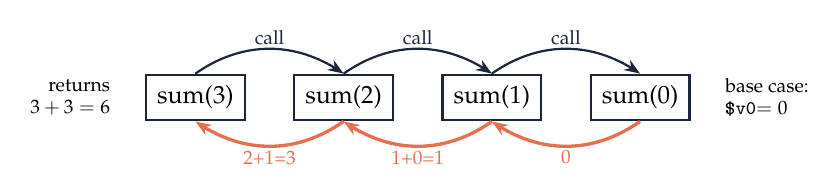
\begin{tikzpicture}[x=1mm,y=1mm,font=\small]
  \node[proc] (a) {sum(3)};
  \node[proc,right=6mm of a] (b) {sum(2)};
  \node[proc,right=6mm of b] (c) {sum(1)};
  \node[proc,right=6mm of c] (d) {sum(0)};
  \draw[wire] (a.north) to[bend left=35] node[above,tk]{call} (b.north);
  \draw[wire] (b.north) to[bend left=35] node[above,tk]{call} (c.north);
  \draw[wire] (c.north) to[bend left=35] node[above,tk]{call} (d.north);
  \draw[newwire] (d.south) to[bend left=35] node[below,tk]{0} (c.south);
  \draw[newwire] (c.south) to[bend left=35] node[below,tk]{1+0=1} (b.south);
  \draw[newwire] (b.south) to[bend left=35] node[below,tk]{2+1=3} (a.south);
  \node[tk,right=4mm of d,align=left] {base case:\\ \ins{\$v0}$=0$};
  \node[tk,left=4mm of a,align=right] {returns\\ $3+3=6$};
\end{tikzpicture}}
\end{solution}

%---------------------------------------------------------------- IS38
\begin{question}{2012--2013 \textbullet\ Q1(a)}{CSE 305 \textbullet\ 10/05/2014 \textbullet\ IS38}{15}
What is a jump address table? Discuss with an appropriate example how Case/Switch Statements can be implemented with a
jump address table.
\end{question}
\begin{solution}
\sub{Jump address table}
A \key{jump address table} (jump table) is an array of words in memory. Entry $k$ holds the \emph{address} of the code
for alternative $k$. To select alternative $k$, the program indexes the table (\texttt{base} $+ 4k$), loads that address
into a register and jumps to it with \ins{jr} (slides: \ins{jr} ``can also be used for computed jumps, e.g.\ for case/switch
statements''). This costs a constant number of instructions for any $k$, whereas a chain of \texttt{if-else} tests
costs up to one compare-and-branch per case.

\sub{Example}
\begin{ccode}
switch (k) {
  case 0: f = i + j; break;
  case 1: f = g + h; break;
  case 2: f = g - h; break;
  case 3: f = i - j; break;
}
\end{ccode}
Assume $f,g,h,i,j,k$ are in \reg{s0}--\reg{s5}, and \reg{t4} holds the base address of \texttt{JumpTable}, whose four words
contain the addresses of labels \texttt{L0}--\texttt{L3}.
\begin{mips}
        sltiu $t3, $s5, 4       # $t3 = (0 <= k < 4) ; unsigned test also rejects k < 0
        beq   $t3, $zero, Exit  # k out of range -> no case matches
        sll   $t1, $s5, 2       # $t1 = 4 * k  (byte offset of entry k)
        add   $t1, $t1, $t4     # $t1 = &JumpTable[k]
        lw    $t0, 0($t1)       # $t0 = JumpTable[k] = address of Lk
        jr    $t0               # jump to the selected case
L0:     add   $s0, $s3, $s4     # k = 0 : f = i + j
        j     Exit              # break
L1:     add   $s0, $s1, $s2     # k = 1 : f = g + h
        j     Exit
L2:     sub   $s0, $s1, $s2     # k = 2 : f = g - h
        j     Exit
L3:     sub   $s0, $s3, $s4     # k = 3 : f = i - j  (last case: no jump needed)
Exit:
\end{mips}
\fig{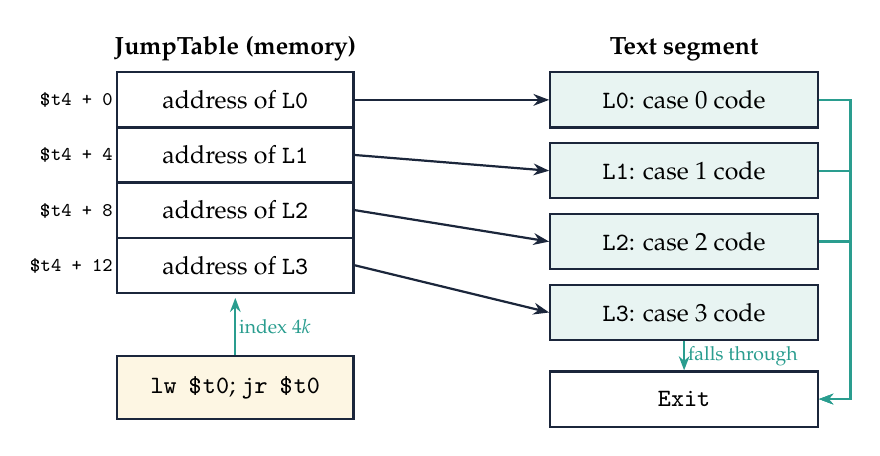
\begin{tikzpicture}[x=1mm,y=1mm,font=\small]
  \foreach \i in {0,1,2,3}{
    \node[blk,minimum width=30mm,minimum height=7mm,anchor=north west] (e\i) at (0,-7*\i) {address of \texttt{L\i}};
    \node[tk,left] at (e\i.west) {\texttt{\$t4 + \the\numexpr4*\i\relax}\ };
    \node[blkm,minimum width=34mm,minimum height=7mm,anchor=north west] (c\i) at (55,-9*\i) {\texttt{L\i}: case \i\ code};
    \draw[wire] (e\i.east) -- (c\i.west);
  }
  \node[font=\small\bfseries,above] at (e0.north) {JumpTable (memory)};
  \node[font=\small\bfseries,above] at (c0.north) {Text segment};
  \node[blkg,minimum width=30mm,anchor=north west] (k) at (0,-36) {\ins{lw \$t0}; \ins{jr \$t0}};
  \draw[ctl] (k.north) -- node[right,tk]{index $4k$} ([yshift=-0.5mm]e3.south);
  \node[blk,minimum width=34mm,minimum height=7mm,anchor=north west] (ex) at (55,-38) {\texttt{Exit}};
  \foreach \i in {0,1,2}{\draw[ctl] (c\i.east) -- ++(4,0) |- (ex.east);}
  \draw[ctl] (c3.south) -- node[right,tk]{falls through} (ex.north);
\end{tikzpicture}}
Every case ends with \ins{j Exit}, which is the \texttt{break}. The range check is required, because an out-of-range
$k$ would load a garbage address. (Two signed tests \ins{slt \$t3,\$s5,\$zero}/\ins{bne} and \ins{slti \$t3,\$s5,4}/\ins{beq}
do the same job as the single \ins{sltiu}.)
\end{solution}

%---------------------------------------------------------------- IS39
\begin{question}{2012--2013 \textbullet\ Q1(b)}{CSE 305 \textbullet\ 10/05/2014 \textbullet\ IS39}{5}
How you can create a 32 bit constant in MIPS Assembly Language?
\end{question}
\begin{solution}
I-format instructions hold only a 16-bit immediate, which covers the common case of small constants. For the occasional 32-bit constant MIPS uses two instructions (slides: ``32-bit Constants''):
\begin{enumerate}
  \item \ins{lui rt, upper16} (\emph{load upper immediate}): copies the 16-bit constant into the \emph{left} 16 bits of rt and clears the right 16 bits to 0.
  \item \ins{ori rt, rt, lower16}: ORs the lower 16 bits in. \ins{ori} \textbf{zero-extends} its immediate, so the upper half is untouched. \ins{addi} should not be used here: it sign-extends, which corrupts the upper half whenever bit 15 is 1.
\end{enumerate}
Example (slides): load \texttt{0000 0000 0111 1101 0000 1001 0000 0000} ($=$\hex{007D0900}) into \reg{s0}:
\begin{mips}
lui  $s0, 61              # $s0 = 0000 0000 0111 1101 0000 0000 0000 0000
ori  $s0, $s0, 2304       # $s0 = 0000 0000 0111 1101 0000 1001 0000 0000
\end{mips}
\fig{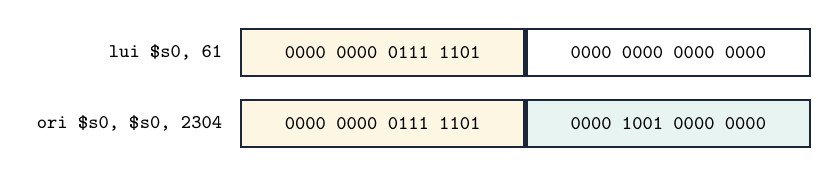
\begin{tikzpicture}[f/.style={draw=ink,thick,minimum height=6mm,minimum width=36mm,font=\scriptsize\ttfamily}]
\node[anchor=east,font=\scriptsize\ttfamily] at (-1mm,0) {lui \$s0, 61};
\node[f,fill=goldbg,anchor=west] (u1) at (0,0) {0000 0000 0111 1101};
\node[f,right=0pt of u1] {0000 0000 0000 0000};
\node[anchor=east,font=\scriptsize\ttfamily] at (-1mm,-9mm) {ori \$s0, \$s0, 2304};
\node[f,fill=goldbg,anchor=west] (u2) at (0,-9mm) {0000 0000 0111 1101};
\node[f,fill=mist,right=0pt of u2] {0000 1001 0000 0000};
\end{tikzpicture}}
The assembler does this automatically for pseudoinstructions such as \ins{li \$s0, 0x007D0900} or \ins{la}, using \reg{at} where needed.
\ans{Use \ins{lui} to put the upper 16 bits in place, then \ins{ori} to insert the lower 16 bits. Example: \ins{lui \$s0,61}; \ins{ori \$s0,\$s0,2304} gives \reg{s0} $=$ \hex{007D0900}.}
\end{solution}

%---------------------------------------------------------------- IS40
\begin{question}{2012--2013 \textbullet\ Q1(c)}{CSE 305 \textbullet\ 10/05/2014 \textbullet\ IS40}{8}
Consider the following MIPS assembly language code and assume that the code fragment is loaded at location
80000 in the memory. What should be the values of the immediate fields of \emph{bne} instruction and \emph{j}
instruction?
\begin{mips}
Loop:   sll  $t1,$s3,2
        add  $t1,$t2,$s6
        Lw   $t0, o($t1)
        bnr  $to,$s5, Exit
        addi $s3, $s3, 1
        j    Loop
Exit:
\end{mips}
\end{question}
\begin{solution}
\sub{Method}
\begin{itemize}
\item \ins{bne} is I-format and uses \key{PC-relative} addressing: the 16-bit field holds
  $\text{offset} = (\text{target} - (\text{PC}_{\text{bne}}+4))/4$ words, because PC has already been incremented by 4.
\item \ins{j} is J-format and uses \key{pseudo-direct} addressing: the 26-bit field holds target$/4$, and the upper 4 bits of
  the target come from PC+4.
\end{itemize}
Each instruction is 4 bytes, so: \ins{sll} 80000, \ins{add} 80004, \ins{lw} 80008, \ins{bne} 80012, \ins{addi} 80016,
\ins{j} 80020, \texttt{Exit} 80024.
\fig{{\small\setlength{\tabcolsep}{4pt}%
\begin{tabular}{r l|c|c|c|c|c|c|}
\cline{3-8}
Addr & Instruction & op & rs & rt & rd & shamt & funct\\ \cline{3-8}
80000 & \ins{Loop: sll \$t1,\$s3,2} & 0 & 0 & 19 & 9 & 2 & 0\\ \cline{3-8}
80004 & \ins{add \$t1,\$t1,\$s6} & 0 & 9 & 22 & 9 & 0 & 32\\ \cline{3-8}
80008 & \ins{lw \$t0,0(\$t1)} & 35 & 9 & 8 & \multicolumn{3}{c|}{0}\\ \cline{3-8}
80012 & \ins{bne \$t0,\$s5,Exit} & 5 & 8 & 21 & \multicolumn{3}{c|}{\key{2}}\\ \cline{3-8}
80016 & \ins{addi \$s3,\$s3,1} & 8 & 19 & 19 & \multicolumn{3}{c|}{1}\\ \cline{3-8}
80020 & \ins{j Loop} & 2 & \multicolumn{5}{c|}{\key{20000}}\\ \cline{3-8}
80024 & \ins{Exit:} & \multicolumn{6}{c|}{\dots}\\ \cline{3-8}
\end{tabular}}}
\ans{bne immediate $=(80024-(80012+4))/4 = 2$; \quad j address field $=80000/4 = 20000$.}
\begin{note}The printed code has typos: \texttt{bnr \$to} is read as \ins{bne \$t0}, \texttt{Lw \$t0, o(\$t1)} as
\ins{lw \$t0, 0(\$t1)}, and \texttt{add \$t1,\$t2,\$s6} is taken as \ins{add \$t1,\$t1,\$s6} (as in the slides). None of
these changes the two immediate fields.\end{note}
\end{solution}

%---------------------------------------------------------------- IS41
\begin{question}{2012--2013 \textbullet\ Q1(d)}{CSE 305 \textbullet\ 10/05/2014 \textbullet\ IS41}{7}
Explain why the assembler might have problems directly implementing the branch instruction in the following code fragment. How can this problem be fixed?
\begin{mips}
Here:  beq $s0, $s2, there
       ...
       ...
there: add $s0, $s0, $s0
\end{mips}
\end{question}
\begin{solution}
\sub{Why there may be a problem}
\ins{beq} is I-format, \fbox{\scriptsize op\,(6)}\fbox{\scriptsize rs\,(5)}\fbox{\scriptsize rt\,(5)}\fbox{\scriptsize offset\,(16)}, and uses PC-relative addressing:
\[\text{target}=(\text{PC}+4)+\text{SignExt}(\text{offset})\times4,\qquad -2^{15}\le\text{offset}\le2^{15}-1 .\]
The ``\ldots'' between \ins{Here} and \ins{there} may contain more than $2^{15}$ (32768) instructions, i.e.\ more than about 128\,KB. In that case the word offset does not fit in 16 bits, and the assembler cannot encode the branch directly.

\sub{Fix (slides: ``Branching far away'')}
Invert the condition, hop over one instruction, and use an unconditional \ins{j}, whose 26-bit field reaches anywhere in the current 256\,MB region:
\begin{mips}
Here:  bne  $s0, $s2, Skip    # opposite test; offset field = 1 (always fits)
       j    there             # pseudodirect: PC[31:28] : addr26 : 00
Skip:  ...                    # continues with the code after the old beq
       ...
there: add  $s0, $s0, $s0
\end{mips}
If \ins{there} were even in a different 256\,MB region (different PC$_{31..28}$), the \ins{j} would be replaced by a register jump: \ins{lui \$at, hi(there)}; \ins{ori \$at, \$at, lo(there)}; \ins{jr \$at}.
\ans{\ins{there} may be more than $2^{15}$ words from PC$+4$, so the 16-bit branch offset overflows. The assembler rewrites the branch as \ins{bne \$s0,\$s2,Skip}; \ins{j there}; \ins{Skip:}. For a target outside the 256\,MB region it uses \ins{lui}/\ins{ori}/\ins{jr}.}
\end{solution}

%---------------------------------------------------------------- IS42
\begin{question}{2011--2012 \textbullet\ Q2(b)}{CSE 305 \textbullet\ 27/07/2013 \textbullet\ IS42}{7.5}
Which instructions and registers are used in procedure call in MIPS hardware? What are the purpose of using these
registers and instructions?
\end{question}
\begin{solution}
\sub{Instructions}
\begin{itemize}
\item \ins{jal ProcedureLabel} (\emph{jump and link}) puts the address of the following instruction (PC$+4$) in \reg{ra} and
  jumps to the procedure, so it does both the call and remembering where to come back.
\item \ins{jr \$ra} (\emph{jump register}) copies \reg{ra} into the PC, which returns to the caller.
  (\ins{jr} with another register is also used for computed jumps, e.g.\ switch tables.)
\item \ins{sw}/\ins{lw} and \ins{addi \$sp,\$sp,$\pm$n} push and pop registers on the stack (procedure frame).
\end{itemize}
\sub{Registers}
\fig{{\small\renewcommand{\arraystretch}{1.12}%
\begin{tabular}{llp{92mm}}
\toprule
Register & Number & Purpose\\ \midrule
\reg{a0}--\reg{a3} & 4--7 & pass the first four arguments to the procedure\\
\reg{v0}, \reg{v1} & 2, 3 & return the result values to the caller\\
\reg{ra} & 31 & return address, written by \ins{jal} and used by \ins{jr}\\
\reg{sp} & 29 & stack pointer: top of the stack, where registers/locals are saved (stack grows down)\\
\reg{fp} & 30 & frame pointer: fixed base of the current procedure frame\\
\reg{gp} & 28 & global pointer to the static data segment\\
\reg{t0}--\reg{t9} & 8--15, 24--25 & temporaries, which the callee may overwrite (the caller saves them if it needs them)\\
\reg{s0}--\reg{s7} & 16--23 & saved registers, which the callee must save and restore if it uses them\\
\bottomrule
\end{tabular}}}
\textbf{Call sequence (slides):} place parameters in \reg{a0}--\reg{a3} $\to$ \ins{jal} transfers control $\to$ callee
acquires storage on the stack (moves \reg{sp}, saves \reg{ra}/\reg{s}-registers) $\to$ performs its task $\to$ puts the
result in \reg{v0}/\reg{v1} $\to$ restores registers and \reg{sp} $\to$ \ins{jr \$ra} returns to the caller.
\end{solution}

%===================================================================== TOPIC 03
\topic{03}{Arithmetic Logic Unit (ALU) Design}

%---------------------------------------------------------------- AL01
\begin{question}{2023--2024 \textbullet\ Q5(b)}{CSE 209 \textbullet\ 29/04/2026 \textbullet\ AL01}{15}
Suppose you want to design a 4-bit ALU where the inputs to the ALU are A $(A_3A_2A_1A_0)$ and B $(B_3B_2B_1B_0)$, and the selection variables are $S_2$, $S_1$, and $S_0$. Also, consider $X_i$, $Y_i$ and $Z_i$ as the inputs to the $i$-th parallel adder of the ALU. The ALU must satisfy the following functional design specification given in Table for Question 5(b) that has to be realized through the parallel adders.
\fig{\begin{tabular}{|c|c|c|c|}\hline
$S_2$ & $S_1$ & $S_0$ & Required Functions\\\hline
0&0&0& $F=A-B-1$\\\hline
0&0&1& $F=A+B+1$\\\hline
0&1&0& $F=$ Transfer $A$\\\hline
0&1&1& $F=$ Decrement $A$\\\hline
1&0&x& $F=A$ OR $B$\\\hline
1&1&x& $F=A'$\\\hline
\end{tabular}}
\begin{center}\small Table for Question 5(b)\end{center}
Devise the input equations ($X_i$, $Y_i$, $Z_i$) for the parallel adders of the ALU.
\end{question}
\begin{solution}
\sub{Method (slides: \emph{ALU Design})}
Each bit $i$ is one full-adder stage with inputs $X_i$, $Y_i$ and carry-in $Z_i$: $F_i=X_i\oplus Y_i\oplus Z_i$, $C_{i+1}=X_iY_i+X_iZ_i+Y_iZ_i$.
\begin{itemize}
\item \key{Arithmetic} ($S_2=0$): $X_i=A_i$. Choose $Y_i\in\{0,B_i,B_i',1\}$ and the input carry $C_0$ so that $F=A+Y+C_0$. For example $A-B-1=A+B'$, $A-1=A+1111$, and $A=A+1111+1$.
\item \key{Logic} ($S_2=1$): kill every carry with $Z_i=S_2'C_i$, so $F_i=X_i\oplus Y_i$. Keep $Y_i$ close to the arithmetic $Y_i$ and modify $X_i$. OR: $X=A+B$, $Y=0$. NOT: $X=A$, $Y=1$.
\end{itemize}
\fig{\small\begin{tabular}{cllll}\toprule
$S_2S_1S_0$ & $F$ & $X_i$ & $Y_i$ & $C_0$\\\midrule
000 & $A-B-1=A+B'$ & $A_i$ & $B_i'$ & 0\\
001 & $A+B+1$ & $A_i$ & $B_i$ & 1\\
010 & Transfer $A$ & $A_i$ & 1 & 1 \quad($A+1111+1=A$)\\
011 & Decrement $A$ & $A_i$ & 1 & 0\\
10x & $A$ OR $B$ & $A_i+B_i$ & 0 & -- ($Z=0$)\\
11x & $A'$ & $A_i$ & 1 & -- ($Z=0$)\\\bottomrule
\end{tabular}}

Transfer $A$ uses $Y=1111$ with carry 1 instead of $Y=0$ with carry 0. This makes $Y_i=1$ whenever $S_1=1$. For $S_2S_1=00$, $Y_i$ is $B_i'$ when $S_0=0$ and $B_i$ when $S_0=1$, i.e.\ $S_0\odot B_i$. For $S_2S_1=10$, $Y_i=0$. $X_i$ differs from $A_i$ only for OR. $C_0=1$ only for rows 001 and 010.
\ans{$X_i=A_i+S_2S_1'B_i$, \quad $Y_i=S_1+S_2'(S_0\odot B_i)$, \quad $C_0=S_1\oplus S_0$, \quad $Z_0=S_2'(S_1\oplus S_0)$, \ $Z_i=S_2'C_i\ (i=1,2,3)$.}
{\small The design was checked by simulating all $(S,A,B)$ combinations.}
\end{solution}

%---------------------------------------------------------------- AL02
\begin{question}{2022--2023 \textbullet\ Q11(a)}{CSE 209 \textbullet\ 13/01/2025 \textbullet\ AL02}{7}
Why is the overflow bit ($V$) computed by XOR-ing the last two carry bits in binary arithmetic operations?
\end{question}
\begin{solution}
In $n$-bit 2's-complement addition, overflow means the true result does not fit in $n$ bits, which can only happen when both operands have the \emph{same} sign and the result sign differs (slides: $+$ve $+$ $+$ve gives sign 1, or $-$ve $+$ $-$ve gives sign 0). Look at the sign-bit (MSB) full adder: inputs $a_{n-1}, b_{n-1}$, carry-in $c_{n-1}$; outputs sum (sign) $s_{n-1}$ and carry-out $c_n$.
\begin{center}\small\begin{tabular}{ccc|cc|l}
\toprule
$a_{n-1}$ & $b_{n-1}$ & $c_{n-1}$ & $s_{n-1}$ & $c_n$ & Case\\
\midrule
0 & 0 & 0 & 0 & 0 & $+$ $+$ $\to$ $+$: fine\\
0 & 0 & 1 & \textcolor{coral}{1} & 0 & $+$ $+$ $\to$ $-$: \textbf{overflow}, $c_{n-1}\ne c_n$\\
0/1 & 1/0 & 0 & 1 & 0 & mixed signs: never overflows, $c_{n-1}=c_n$\\
0/1 & 1/0 & 1 & 0 & 1 & mixed signs: never overflows, $c_{n-1}=c_n$\\
1 & 1 & 0 & \textcolor{coral}{0} & 1 & $-$ $-$ $\to$ $+$: \textbf{overflow}, $c_{n-1}\ne c_n$\\
1 & 1 & 1 & 1 & 1 & $-$ $-$ $\to$ $-$: fine\\
\bottomrule
\end{tabular}\end{center}
\begin{itemize}
\item Both operands positive $\Rightarrow c_n = 0$ always; the sign becomes wrongly 1 exactly when a carry \emph{enters} the sign bit ($c_{n-1}=1$).
\item Both negative $\Rightarrow c_n = 1$ always; the sign becomes wrongly 0 exactly when \emph{no} carry enters ($c_{n-1}=0$).
\item Mixed signs $\Rightarrow c_n = c_{n-1}$ always, and no overflow is possible.
\end{itemize}
So overflow $\iff$ carry into the sign bit $\ne$ carry out of it, i.e.\ $V = c_{n-1}\oplus c_n$ (in the slides' 8-bit ALU, $V = C_8\oplus C_9$). One XOR gate replaces a comparison of three sign bits, and it works for subtraction too because $A-B$ is done as $A+\overline{B}+1$.
Example (4-bit): $0111+0001 = 1000$ ($7+1\ne-8$): $c_3=1$, $c_4=0$ $\Rightarrow V=1$.
\ans{Because overflow in 2's-complement occurs exactly when the carry into the MSB differs from the carry out of the MSB: $V = C_{n-1}\oplus C_n$.}
\end{solution}

%---------------------------------------------------------------- AL03
\begin{question}{2022--2023 \textbullet\ Q11(d)}{CSE 209 \textbullet\ 13/01/2025 \textbullet\ AL03}{10}
Design a 4-bit Arithmetic Logic Unit (ALU) with three selection variables, $S_0$, $S_1$, and $S_2$. These selecting variables control the ALU to perform various operations on two 4-bit inputs, labeled as A and B. Derive the input equations ($X_i$, $Y_i$, and $Z_i$) for the parallel adders used in the ALU that satisfy the following functional design specifications, (where X means don't care).
\fig{\begin{tabular}{|c|c|c|l|}\hline
$S_2$ & $S_1$ & $S_0$ & \textbf{Required Operation}\\\hline
0&0&0& $-A-B-2$\\\hline
0&0&1& Add 1's complement of A to B\\\hline
0&1&0& $A+B$\\\hline
0&1&1& $A-B$\\\hline
1&0&x& A AND B\\\hline
1&1&x& A XOR B\\\hline
\end{tabular}}
\end{question}
\begin{solution}
\sub{Method (slides: \emph{ALU Design})}
Each bit $i$ is one full-adder stage with inputs $X_i$, $Y_i$ and carry-in $Z_i$: $F_i=X_i\oplus Y_i\oplus Z_i$, $C_{i+1}=X_iY_i+X_iZ_i+Y_iZ_i$.
\begin{itemize}
\item \key{Arithmetic} ($S_2=0$): $F=X+Y+C_0$ with $X_i\in\{A_i,A_i'\}$, $Y_i\in\{B_i,B_i'\}$ and input carry $C_0$. In 2's complement $-A=A'+1$, so $-A-B-2=(A'+1)+(B'+1)-2=A'+B'$ and $A-B=A+B'+1$.
\item \key{Logic} ($S_2=1$): kill every carry with $Z_i=S_2'C_i$, so $F_i=X_i\oplus Y_i$. XOR: $X=A$, $Y=B$. AND: $X=A+B'$, $Y=B'$, since $(A+B')\oplus B'=AB$.
\end{itemize}
\fig{\small\begin{tabular}{cllll}\toprule
$S_2S_1S_0$ & $F$ & $X_i$ & $Y_i$ & $C_0$\\\midrule
000 & $-A-B-2=A'+B'$ & $A_i'$ & $B_i'$ & 0\\
001 & $A'+B$ & $A_i'$ & $B_i$ & 0\\
010 & $A+B$ & $A_i$ & $B_i$ & 0\\
011 & $A-B=A+B'+1$ & $A_i$ & $B_i'$ & 1\\
10x & AND & $A_i+B_i'$ & $B_i'$ & -- ($Z=0$)\\
11x & XOR & $A_i$ & $B_i$ & -- ($Z=0$)\\\bottomrule
\end{tabular}}

$X_i$ is $A_i'$ when $S_2S_1=00$ and $A_i$ otherwise, plus the AND term. So $X_i=(A_i\oplus S_2'S_1')+S_2S_1'B_i'$.
$Y_i$, in the order $000,001,010,011,10x,11x$, is $B',B,B,B',B',B$. So $B_i$ is complemented exactly when $S_1'\oplus S_2'S_0=1$.
\ans{$X_i=(A_i\oplus S_2'S_1')+S_2S_1'B_i'$, \quad $Y_i=B_i\oplus S_1'\oplus S_2'S_0$, \quad $C_0=S_1S_0$, \quad $Z_0=S_2'S_1S_0$, \ $Z_i=S_2'C_i\ (i=1,2,3)$.}
{\small The design was checked by simulating all $(S,A,B)$ combinations.}
\end{solution}

%---------------------------------------------------------------- AL04
\begin{question}{2022--2023 \textbullet\ Q5(b)}{CSE 305 \textbullet\ 25/04/2024 \textbullet\ AL04}{14}
Howard wants to demonstrate his engineering skills, but Sheldon sets a challenging constraint for him. Howard is tasked with designing a 4-bit Arithmetic Logic Unit (ALU), and the constraint is that he cannot use any parallel adder. Instead, he is only allowed to use parallel subtractors and logic gates for the ALU design. The ALU should have three selection variables, denoted as S0, S1, and S2. These selection variables control the ALU to perform various operations on two 4-bit inputs, Labelled as A and B. Your task is to help Howard design the 4-bit Arithmetic Logic Unit (ALU) so that it can do the following operations:
\fig{\begin{tabular}{|c|c|c|c|}\hline
$S_2$ & $S_1$ & $S_0$ & \textit{Operation}\\\hline
0&0&0& A $-$ B\\\hline
0&0&1& A $+$ B\\\hline
0&1&0& $-$A $-$B $-$ 2\\\hline
0&1&1& B $-$ A\\\hline
1&0&0& A XOR B\\\hline
1&1&0& A AND B\\\hline
\end{tabular}}
\end{question}
\begin{solution}
\sub{Method: the ALU-design approach (slides) with a parallel \emph{subtractor}}
This follows the slides' Xi/Yi/Zi method, with a parallel subtractor in place of the adder. Each bit $i$ is a full-subtractor stage with inputs $X_i$, $Y_i$ and borrow-in $Z_i$:
\[D_i=X_i\oplus Y_i\oplus Z_i,\qquad b_{i+1}=X_i'Y_i+X_i'Z_i+Y_iZ_i,\qquad\text{4-bit result } D=X-Y-b_0 .\]
\begin{itemize}
\item \key{Arithmetic} ($S_2=0$): rewrite each operation as $X-Y-b_0$ with $X\in\{A,A'\}$, $Y\in\{B,B'\}$, using $-A=A'+1$ (2's complement):
\[\begin{gathered}A+B=A-(B'+1)=A-B'-1,\qquad -A-B-2=(A'+1)-B-2=A'-B-1,\\ B-A=(-A-1)-(-B-1)=A'-B'.\end{gathered}\]
\item \key{Logic} ($S_2=1$): the difference bit is the same XOR as an adder's sum bit. Killing every borrow ($Z_i=S_2'b_i$) gives $D_i=X_i\oplus Y_i$. XOR: $X=A$, $Y=B$. AND: $X=A+B'$, $Y=B'$, since $(A+B')\oplus B'=AB$.
\end{itemize}
\fig{\small\begin{tabular}{cllll}\toprule
$S_2S_1S_0$ & $F$ & $X_i$ & $Y_i$ & $b_0$\\\midrule
000 & $A-B$ & $A_i$ & $B_i$ & 0\\
001 & $A+B=A-B'-1$ & $A_i$ & $B_i'$ & 1\\
010 & $-A-B-2=A'-B-1$ & $A_i'$ & $B_i$ & 1\\
011 & $B-A=A'-B'$ & $A_i'$ & $B_i'$ & 0\\
100 & XOR & $A_i$ & $B_i$ & -- ($Z=0$)\\
110 & AND & $A_i+B_i'$ & $B_i'$ & -- ($Z=0$)\\
101, 111 & unused (don't care) &&&\\\bottomrule
\end{tabular}}

$X_i$ is complemented when $S_2S_1=01$, and $B_i'$ is ORed in for AND ($S_2S_1=11$). $Y_i$ is $B_i'$ in rows 001, 011 and 110. Using the don't-care rows, the complement condition becomes $S_0+S_2S_1$.
\ans{$X_i=(A_i\oplus S_2'S_1)+S_2S_1B_i'$, \quad $Y_i=B_i\oplus(S_0+S_2S_1)$, \quad $b_0=S_1\oplus S_0$, \quad $Z_0=S_2'(S_1\oplus S_0)$, \ $Z_i=S_2'\,b_i$ ($b_i$ = borrow-out of stage $i-1$).}
\begin{note}The question does not say how the subtractor's borrow is modelled. We take the standard full subtractor, $D=X-Y-b_{\text{in}}$. Rows 101 and 111 are not in the table, so we treat them as don't-cares.\end{note}
{\small The design was checked by simulating all $(S,A,B)$ combinations.}
\end{solution}

%---------------------------------------------------------------- AL05
\begin{question}{2020--2021 \textbullet\ Q10(b)}{CSE 305 \textbullet\ 24/09/2022 \textbullet\ AL05}{18}
Suppose you want to design a 4-bit ALU where the inputs to the ALU are A $(A_3A_2A_1A_0)$ and B $(B_3B_2B_1B_0)$, and the selection variables are $S_3$, $S_2$, $S_1$ and $S_0$. Also, consider $X_i$, $Y_i$ and $Z_i$ as the inputs to the $i$-th parallel adder of the ALU. The ALU must satisfy the following functional design specification (given in Table 10b) that has to be realized through the parallel adders. Your task is to derive the input equations ($X_i$, $Y_i$ and $Z_i$) for the parallel adders of the ALU. You must design using the least possible number of gates.
\fig{\begin{tabular}{|c|c|c|c|l|}\hline
$S_3$ & $S_2$ & $S_1$ & $S_0$ & Required Functions\\\hline
0&0&0&0& $F=A$\\\hline
0&0&0&1& $F=A-1$\\\hline
0&0&1&0& $F=A+B+1$\\\hline
0&0&1&1& $F=A+B$\\\hline
0&1&0&0& $F=A-B$\\\hline
0&1&0&1& $F=A-B-1$\\\hline
0&1&1&0& $F=A+1$\\\hline
0&1&1&1& $F=A$\\\hline
1&0&0&X& $F=A'$\\\hline
1&0&1&X& $F=AB'$\\\hline
1&1&0&X& $F=A\odot B$ [XNOR]\\\hline
1&1&1&X& $F=A\vee B$ [OR]\\\hline
\end{tabular}}
\begin{center}\small\textbf{Table 10(b): Required functional design specification}\end{center}
\end{question}
\begin{solution}
\sub{Method (slides: \emph{ALU Design})}
Each bit $i$ is one full-adder stage with inputs $X_i$, $Y_i$ and carry-in $Z_i$: $F_i=X_i\oplus Y_i\oplus Z_i$, $C_{i+1}=X_iY_i+X_iZ_i+Y_iZ_i$.
\begin{itemize}
\item \key{Arithmetic} ($S_3=0$): $X_i=A_i$. Choose $Y_i\in\{0,B_i,B_i',1\}$ and the input carry $C_0$ so that $F=A+Y+C_0$ (e.g.\ $A-B=A+B'+1$, $A-1=A+1111$).
\item \key{Logic} ($S_3=1$): kill every carry with $Z_i=S_3'C_i$, so $F_i=X_i\oplus Y_i$. Choose the $(X_i,Y_i)$ pair that \emph{reuses} the arithmetic $Y_i$ for the same $S_2S_1$, to save gates. NOT: $(A,1)$. $AB'$: $(A{+}B,\,B)$, since $(A+B)\oplus B=AB'$. XNOR: $(A,B')$. OR: $(A{+}B,\,0)$.
\end{itemize}
Every arithmetic row uses $X_i=A_i$. $Y_i$ depends on $S_2S_1$: $00\to S_0$ ($A$ / $A-1$), $01\to B_i$, $10\to B_i'$, $11\to 0$. For row 0111 ($F=A$) we choose $Y=0$, $C_0=0$ so that $11\to0$ holds for both values of $S_0$.

\fig{\small\begin{tabular}{cllll}\toprule
$S_3S_2S_1S_0$ & $F$ & $X_i$ & $Y_i$ & $C_0$\\\midrule
0000 / 0001 & $A$ / $A-1$ & $A_i$ & 0 / 1 & 0\\
0010 / 0011 & $A+B+1$ / $A+B$ & $A_i$ & $B_i$ & 1 / 0\\
0100 / 0101 & $A-B$ / $A-B-1$ & $A_i$ & $B_i'$ & 1 / 0\\
0110 / 0111 & $A+1$ / $A$ & $A_i$ & 0 & 1 / 0\\
100x & $A'$ & $A_i$ & 1 & --\\
101x & $AB'$ & $A_i+B_i$ & $B_i$ & --\\
110x & XNOR & $A_i$ & $B_i'$ & --\\
111x & OR & $A_i+B_i$ & 0 & --\\\bottomrule
\end{tabular}}

$X_i$ changes only when $S_3S_1=11$. $Y_i$ is a 4-to-1 selection on $S_2S_1$ of $(S_0+S_3,\;B_i,\;B_i',\;0)$. $C_0=1$ only for 0010, 0100 and 0110.
\ans{$X_i=A_i+S_3S_1B_i$, \quad $Y_i=S_2'S_1'(S_0+S_3)+S_2'S_1B_i+S_2S_1'B_i'$, \quad $C_0=S_0'(S_1+S_2)$, \quad $Z_0=S_3'S_0'(S_1+S_2)$, \ $Z_i=S_3'C_i\ (i=1,2,3)$.}
\begin{note}In the scan of Table 10(b), the ``B'' in rows $A+B$ and $A-B$ is a degraded glyph that looks like ``6''. We read it as B. The $S_3$ column header is handwritten in the scan.\end{note}
{\small The design was checked by simulating all $(S,A,B)$ combinations.}
\end{solution}

%---------------------------------------------------------------- AL06
\begin{question}{2020--2021 \textbullet\ Q12(d)}{CSE 305 \textbullet\ 24/09/2022 \textbullet\ AL06}{8}
Consider the following module.
\fig{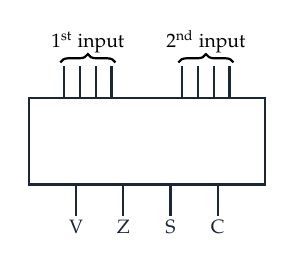
\begin{tikzpicture}[font=\small]
\node[blk,minimum width=30mm,minimum height=11mm] (M) at (0,0) {};
\foreach \x in {-1.05,-0.85,-0.65,-0.45,0.45,0.65,0.85,1.05}{\draw[thick,ink] (\x,0.55)--(\x,0.95);}
\draw[decorate,decoration={brace,amplitude=3pt},thick] (-1.1,1.0)--(-0.4,1.0) node[midway,above=2pt,tk]{1$^{\text{st}}$ input};
\draw[decorate,decoration={brace,amplitude=3pt},thick] (0.4,1.0)--(1.1,1.0) node[midway,above=2pt,tk]{2$^{\text{nd}}$ input};
\foreach \x/\l in {-0.9/V,-0.3/Z,0.3/S,0.9/C}{\draw[thick,ink] (\x,-0.55)--(\x,-0.95) node[below,tk]{\l};}
\end{tikzpicture}}
This module takes two 4-bit inputs, and shows only the four status bits (V: Overflow, Z: Zero, S: Sign and C: Carry) considering the subtraction operation of the second input from the first input. If the first 4-bit input is expressed by A and second 4-bit input is expressed by B, draw the diagram of the complete circuit that can determine whether A$>$B, A$=$B, or A$<$B.
\end{question}
\begin{solution}
\sub{Reading the status bits after $A - B$ (Mano, ALU status register)}
The module computes $A + \overline{B} + 1$. $Z=1$ iff $A=B$. For \key{signed} (2's-complement) numbers the true sign of $A-B$ is $S\oplus V$ (the sign bit is wrong exactly when overflow occurred); for \key{unsigned} numbers $C=1$ means no borrow, i.e.\ $A\ge B$.
\begin{center}\small\begin{tabular}{lll}
\toprule
Relation & signed (2's complement) & unsigned\\
\midrule
$A<B$ & $S\oplus V = 1$ & $C=0$ (borrow)\\
$A=B$ & $Z=1$ & $Z=1$\\
$A>B$ & $(S\oplus V)'\cdot Z' = (S\oplus V + Z)'$ & $C\cdot Z'$\\
\bottomrule
\end{tabular}\end{center}
Assuming signed 4-bit operands: $A<B = S\oplus V$, \ $A=B = Z$, \ $A>B = \overline{(S\oplus V)+Z}$ (one XOR $+$ one NOR).
\fig{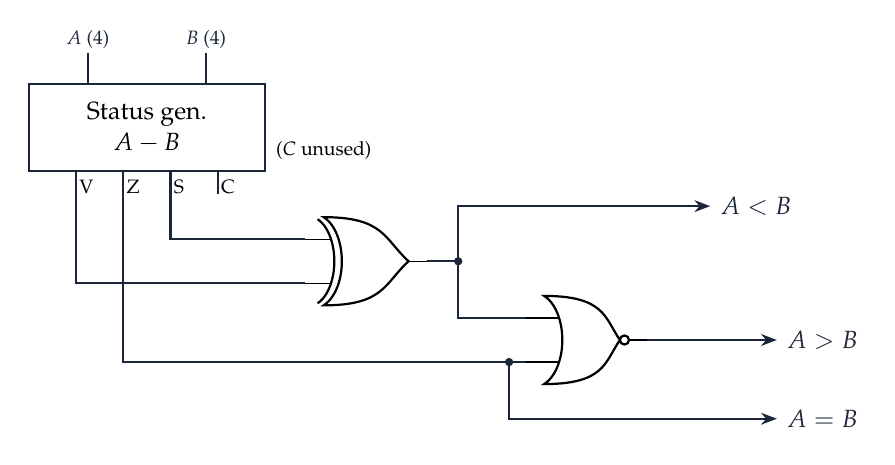
\begin{tikzpicture}[font=\small]
\node[blk,minimum width=30mm,minimum height=11mm,align=center] (M) at (0,0) {Status gen.\\$A-B$};
\draw[thick,ink] (-0.75,0.55)--(-0.75,0.95) node[above,tk]{$A$ (4)};
\draw[thick,ink] (0.75,0.55)--(0.75,0.95) node[above,tk]{$B$ (4)};
\foreach \x/\l in {-0.9/V,-0.3/Z,0.3/S,0.9/C}{\draw[thick,ink] (\x,-0.55)--(\x,-0.85); \node[tk,anchor=west] at (\x,-0.75) {\l};}
\node[xor port] (X) at (3.4,-1.7) {};
\node[nor port] (N) at (6.2,-2.7) {};
\draw[thick,ink] (0.3,-0.85) |- (X.in 1);
\draw[thick,ink] (-0.9,-0.85) |- (X.in 2);
\draw[thick,ink] (X.out) -- ++(0.4,0) coordinate (xo) |- (N.in 1);
\fill[ink] (xo) circle (1.5pt);
\draw[wire] (xo) -- ++(0,0.7) -- ++(3.2,0) node[right]{$A<B$};
\draw[thick,ink] (-0.3,-0.85) |- (N.in 2);
\fill[ink] (4.6,0 |- N.in 2) circle (1.5pt);
\draw[wire] (4.6,0 |- N.in 2) |- (8.0,-3.7) node[right]{$A=B$};
\draw[wire] (N.out) -- (8.0,0 |- N.out) node[right]{$A>B$};
\node[tk,anchor=west] at (1.6,-0.3) {($C$ unused)};
\end{tikzpicture}}
\ans{$A<B = S\oplus V$; \ $A=B = Z$; \ $A>B = \overline{(S\oplus V)+Z}$ (signed). For unsigned inputs: $A<B=\overline{C}$, $A=B=Z$, $A>B=C\cdot\overline{Z}$.}
\end{solution}

%---------------------------------------------------------------- AL07
\begin{question}{2019--2020 \textbullet\ Q2(a)}{CSE 305 \textbullet\ 18/09/2021 \textbullet\ AL07}{20}
Suppose you want to design a 4-bit ALU where the inputs to the ALU are A $(A_3A_2A_1A_0)$ and B $(B_3B_2B_1B_0)$, and the selection variables are $S_3, S_2, S_1$ and $S_0$. Also, consider $X_i, Y_i$ and $Z_i$ as the inputs to the $i^{th}$ parallel adder of the ALU. The ALU must satisfy the following functional design specification (given in Table 2a) that has to be realized through the parallel adders. Your task is to derive the input equations ($X_i, Y_i$ and $Z_i$) for the parallel adders of the ALU. You must design using the least possible number of gates.
\fig{\begin{tabular}{|c|c|c|c|l|}\hline
$S_3$ & $S_2$ & $S_1$ & $S_0$ & \textbf{Required Functions}\\\hline
0&0&0&0& $F=A'$\\\hline
0&0&0&1& $F=A'+1$\\\hline
0&0&1&0& $F=A'+B$\\\hline
0&0&1&1& $F=A'+B+1$\\\hline
0&1&0&0& $F=A'-B-1$\\\hline
0&1&0&1& $F=A'-B$\\\hline
0&1&1&0& $F=A'-1$\\\hline
0&1&1&1& $F=A'$\\\hline
1&0&0&x& $F=(AB)'$ [NAND]\\\hline
1&0&1&x& $F=A\odot B$ [XNOR]\\\hline
1&1&0&x& $F=A\oplus B$ [XOR]\\\hline
1&1&1&x& $F=A\vee B$ [OR]\\\hline
\end{tabular}}
\begin{center}\small\textbf{Table 2a: Required Functional design specification}\end{center}
\end{question}
\begin{solution}
\sub{Method (slides: \emph{ALU Design})}
Each bit $i$ is one full-adder stage with inputs $X_i$, $Y_i$ and carry-in $Z_i$: $F_i=X_i\oplus Y_i\oplus Z_i$, $C_{i+1}=X_iY_i+X_iZ_i+Y_iZ_i$.
\begin{itemize}
\item \key{Arithmetic} ($S_3=0$): this is exactly the slides' Table 9-1, but with $X_i=A_i'$. $Y_i$ is selected by $S_2S_1$: $00\to0$, $01\to B$, $10\to B'$, $11\to1111$, giving $Y_i=S_1B_i+S_2B_i'$. $S_0$ is the input carry: $C_0=S_0$. (Check: $A'-B-1=A'+B'$, $A'-B=A'+B'+1$, $A'-1=A'+1111$, $A'=A'+1111+1$.)
\item \key{Logic} ($S_3=1$): kill every carry with $Z_i=S_3'C_i$, so $F_i=X_i\oplus Y_i$. To save gates, keep the same $Y_i$ and solve $X_i\oplus Y_i=F_i$ for $X_i$.
\end{itemize}
\fig{\small\begin{tabular}{cllll}\toprule
$S_3S_2S_1$ & $F$ & $Y_i$ (fixed) & required $X_i$ & check\\\midrule
100 & NAND & 0 & $A_i'+B_i'$ & $=(AB)'$\\
101 & XNOR & $B_i$ & $A_i'$ & $A'\oplus B=A\odot B$\\
110 & XOR & $B_i'$ & $A_i'$ & $A'\oplus B'=A\oplus B$\\
111 & OR & 1 & $A_i'B_i'$ & $(A'B')'=A+B$\\\bottomrule
\end{tabular}}

So $X_i=A_i'$ everywhere except two rows. Let $K=S_3S_2S_1$ and $M=S_3S_2'S_1'$; each is one gate, shared by all four stages. Then $X_i=A_i'(KB_i)'+MB_i'$.
\ans{$X_i=A_i'\,(S_3S_2S_1B_i)'+S_3S_2'S_1'B_i'$, \quad $Y_i=S_1B_i+S_2B_i'$, \quad $C_0=S_0$, \quad $Z_0=S_3'S_0$, \ $Z_i=S_3'C_i\ (i=1,2,3)$.}
{\small The design was checked by simulating all $(S,A,B)$ combinations.}
\end{solution}

%---------------------------------------------------------------- AL08
\begin{question}{2019--2020 \textbullet\ Q2(b)}{CSE 305 \textbullet\ 18/09/2021 \textbullet\ AL08}{15}
Suppose, you want to implement a hardware unit that would produce the value of $F$ using the following logic (the logic is given in C syntax).
\begin{ccode}
if ((A>=B && C!=D) || X==0)
      F=1;
else
      F=0
\end{ccode}
Here, each of the variables $A, B, C, D$ and $X$ is of 4-bits where the variable $F$ is of 1-bit. After searching the hardware stationaries, you bought some basic gates. Also, you bought some status-generator modules (see Figure 2b) each of which takes two 4-bit inputs, and shows only the four status bits (V: Overflow, Z: Zero, S: Sign and C: Carry) considering the subtraction operation of the 2$^{\text{nd}}$ input from the 1$^{\text{st}}$ input.
\fig{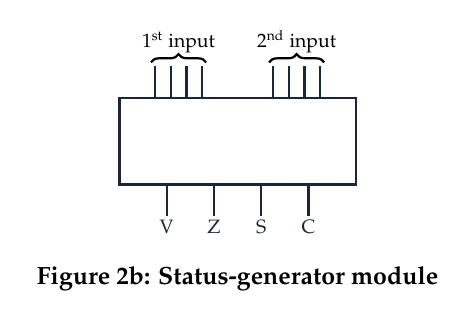
\begin{tikzpicture}[font=\small]
\node[blk,minimum width=30mm,minimum height=11mm] (M) at (0,0) {};
\foreach \x in {-1.05,-0.85,-0.65,-0.45,0.45,0.65,0.85,1.05}{\draw[thick,ink] (\x,0.55)--(\x,0.95);}
\draw[decorate,decoration={brace,amplitude=3pt},thick] (-1.1,1.0)--(-0.4,1.0) node[midway,above=2pt,tk]{1$^{\text{st}}$ input};
\draw[decorate,decoration={brace,amplitude=3pt},thick] (0.4,1.0)--(1.1,1.0) node[midway,above=2pt,tk]{2$^{\text{nd}}$ input};
\foreach \x/\l in {-0.9/V,-0.3/Z,0.3/S,0.9/C}{\draw[thick,ink] (\x,-0.55)--(\x,-0.95) node[below,tk]{\l};}
\node[below=9mm of M,font=\small\bfseries] {Figure 2b: Status-generator module};
\end{tikzpicture}}
Now, (just) draw the circuit diagram of the full hardware unit using basic gates and status-generator modules.
\end{question}
\begin{solution}
\sub{Reading the status bits after $P - Q$ (Mano, ALU status register)}
A module computes $P + \overline{Q} + 1$. $Z=1$ iff $P=Q$, so $P\ne Q = Z'$. For \key{signed} (2's-complement) numbers the true sign of $P-Q$ is $S\oplus V$, so $P\ge Q \iff S\oplus V = 0$; for \key{unsigned} numbers $P\ge Q \iff C=1$ (no borrow). Comparing $X$ with the constant $0000$ gives $X==0 \iff Z=1$.

\sub{Design (signed 4-bit operands assumed)}
Use three modules: M1 on $(A,B)$, M2 on $(C,D)$, M3 on $(X, 0000)$.
\[ A\ge B = (S_1\oplus V_1)',\qquad C\ne D = Z_2',\qquad X==0 \;=\; Z_3 \]
\[ F = (S_1\oplus V_1)'\cdot Z_2' + Z_3 = \overline{(S_1\oplus V_1) + Z_2} + Z_3 \]
So one XOR, one NOR and one OR gate suffice.
\fig{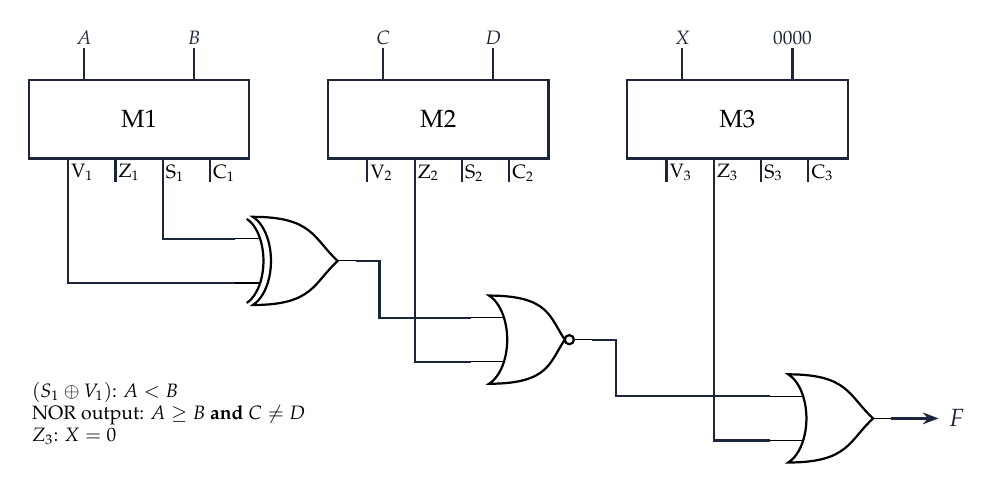
\begin{tikzpicture}[font=\small]
\foreach \n/\cx/\p/\q in {1/0/A/B,2/3.8/C/D,3/7.6/X/0000}{
 \node[blk,minimum width=28mm,minimum height=10mm] (M\n) at (\cx,0) {M\n};
 \draw[thick,ink] (\cx-0.7,0.5)--(\cx-0.7,0.9) node[above,tk]{$\p$};
 \draw[thick,ink] (\cx+0.7,0.5)--(\cx+0.7,0.9) node[above,tk]{$\q$};
 \foreach \dx/\l in {-0.9/V,-0.3/Z,0.3/S,0.9/C}{\draw[thick,ink] (\cx+\dx,-0.5)--(\cx+\dx,-0.8); \node[tk,anchor=west] at (\cx+\dx,-0.68) {\l$_\n$};}}
\node[xor port] (X) at (2.6,-1.8) {};
\node[nor port] (N) at (5.6,-2.8) {};
\node[or port] (O) at (9.4,-3.8) {};
\draw[thick,ink] (0.3,-0.8) |- (X.in 1);
\draw[thick,ink] (-0.9,-0.8) |- (X.in 2);
\draw[thick,ink] (X.out) -- ++(0.3,0) |- (N.in 1);
\draw[thick,ink] (3.5,-0.8) |- (N.in 2);
\draw[thick,ink] (N.out) -- ++(0.3,0) |- (O.in 1);
\draw[thick,ink] (7.3,-0.8) |- (O.in 2);
\draw[wire] (O.out) -- ++(0.6,0) node[right]{$F$};
\node[tk,align=left,anchor=north west] at (-1.4,-3.3) {$(S_1\oplus V_1)$: $A<B$\\NOR output: $A\ge B$ \textbf{and} $C\ne D$\\$Z_3$: $X=0$};
\end{tikzpicture}}
\ans{$F = \overline{(S_1\oplus V_1)+Z_2} + Z_3$ (signed). For unsigned $A,B$: $F = C_1\cdot\overline{Z_2} + Z_3$.}
\end{solution}

%---------------------------------------------------------------- AL09
\begin{question}{2018--2019 \textbullet\ Q5(d)}{CSE 305 \textbullet\ 29/10/2019 \textbullet\ AL09}{10}
Design a 4-bit ALU with three selection variables $S_0$, $S_1$ and $S_2$ that performs the following operations on two 4-bit inputs (A and B):
\fig{\begin{tabular}{|c|c|c|c|}\hline
$S_2$ & $S_1$ & $S_0$ & \textbf{Operation}\\\hline
0&0&0& Addition\\\hline
0&0&1& Transfer A\\\hline
0&1&0& Add 1's complement of B to A\\\hline
0&1&1& Increment A\\\hline
1&0&0& XOR\\\hline
1&0&1& NOT\\\hline
1&1&0& AND\\\hline
1&1&1& OR\\\hline
\end{tabular}}
Draw the logic diagram of one typical stage of your designed ALU.
\end{question}
\begin{solution}
\sub{Method (slides: \emph{ALU Design})}
Each bit $i$ is one full-adder stage with inputs $X_i$, $Y_i$ and carry-in $Z_i$: $F_i=X_i\oplus Y_i\oplus Z_i$, $C_{i+1}=X_iY_i+X_iZ_i+Y_iZ_i$.
\begin{itemize}
\item \key{Arithmetic} ($S_2=0$): $X_i=A_i$. Choose $Y_i\in\{0,B_i,B_i',1\}$ and the input carry $C_0$ so that $F=A+Y+C_0$.
\item \key{Logic} ($S_2=1$): kill every carry with $Z_i=S_2'C_i$, so $F_i=X_i\oplus Y_i$. Keep $Y_i$ close to the arithmetic $Y_i$ and modify $X_i$. XOR: $(A,B)$. NOT: $(A,1)$. AND: $(A{+}B',\,B')$. OR: $(A{+}B,\,0)$.
\end{itemize}
\fig{\small\begin{tabular}{cllll}\toprule
$S_2S_1S_0$ & $F$ & $X_i$ & $Y_i$ & $C_0$\\\midrule
000 & $A+B$ & $A_i$ & $B_i$ & 0\\
001 & Transfer $A$ & $A_i$ & 1 & 1 \quad($A+1111+1=A$)\\
010 & $A+B'$ & $A_i$ & $B_i'$ & 0\\
011 & $A+1$ & $A_i$ & 0 & 1\\
100 & XOR & $A_i$ & $B_i$ & --\\
101 & NOT & $A_i$ & 1 & --\\
110 & AND & $A_i+B_i'$ & $B_i'$ & --\\
111 & OR & $A_i+B_i$ & 0 & --\\\bottomrule
\end{tabular}}

Transfer $A$ uses $(Y{=}1,\,C_0{=}1)$ instead of $(Y{=}0,\,C_0{=}0)$. This makes $Y_i$ independent of $S_2$: $S_1S_0=00\to B$, $01\to1$, $10\to B'$, $11\to0$. $C_0=1$ exactly when $S_2'S_0=1$.
\ans{$X_i=A_i+S_2S_1(S_0\odot B_i)$, \quad $Y_i=S_0'(S_1\oplus B_i)+S_1'S_0$, \quad $C_0=S_0$, \quad $Z_i=S_2'C_i$ (so $Z_0=S_2'S_0$).}
\textbf{One typical stage:}
\fig{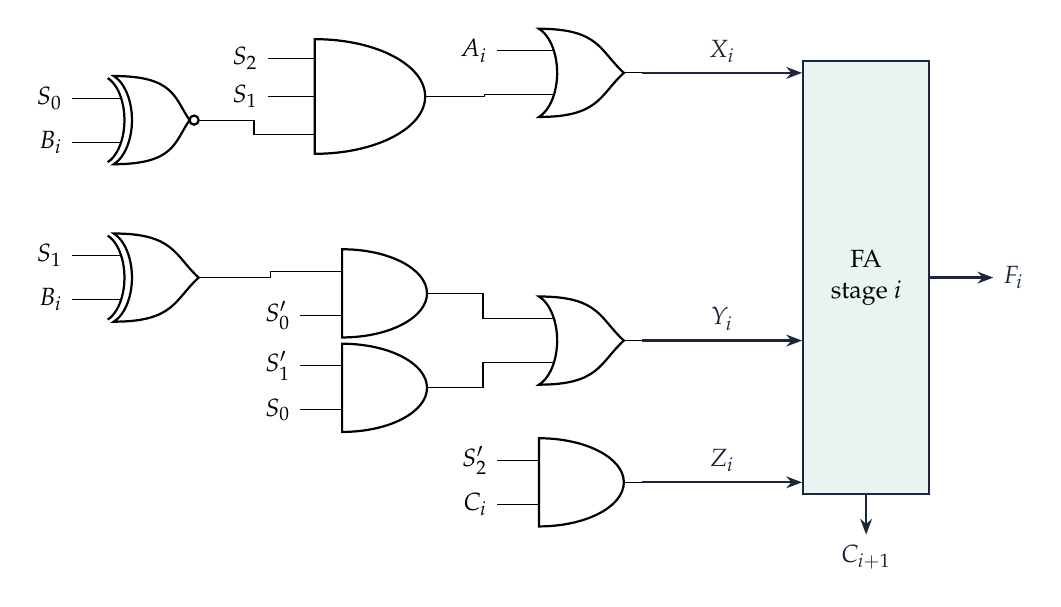
\begin{tikzpicture}[font=\small]
\node[xnor port] (g1) at (0,4) {};
\draw (g1.in 1) -- ++(-0.3,0) node[left]{$S_0$};
\draw (g1.in 2) -- ++(-0.3,0) node[left]{$B_i$};
\node[and port, number inputs=3, scale=1.3] (g2) at (2.9,4.3) {};
\draw (g2.in 1) -- ++(-0.3,0) node[left]{$S_2$};
\draw (g2.in 2) -- ++(-0.3,0) node[left]{$S_1$};
\draw (g1.out) -| ($(g1.out)!0.5!(g2.in 3)$) |- (g2.in 3);
\node[or port] (g3) at (5.4,4.6) {};
\draw (g3.in 1) -- ++(-0.3,0) node[left]{$A_i$};
\draw (g2.out) -| ($(g2.out)!0.5!(g3.in 2)$) |- (g3.in 2);
\node[xor port] (g4) at (0,2) {};
\draw (g4.in 1) -- ++(-0.3,0) node[left]{$S_1$};
\draw (g4.in 2) -- ++(-0.3,0) node[left]{$B_i$};
\node[and port] (g5) at (2.9,1.8) {};
\draw (g4.out) -| ($(g4.out)!0.5!(g5.in 1)$) |- (g5.in 1);
\draw (g5.in 2) -- ++(-0.3,0) node[left]{$S_0'$};
\node[and port] (g6) at (2.9,0.6) {};
\draw (g6.in 1) -- ++(-0.3,0) node[left]{$S_1'$};
\draw (g6.in 2) -- ++(-0.3,0) node[left]{$S_0$};
\node[or port] (g7) at (5.4,1.2) {};
\draw (g5.out) -| ($(g5.out)!0.5!(g7.in 1)$) |- (g7.in 1);
\draw (g6.out) -| ($(g6.out)!0.5!(g7.in 2)$) |- (g7.in 2);
\node[and port] (g8) at (5.4,-0.6) {};
\draw (g8.in 1) -- ++(-0.3,0) node[left]{$S_2'$};
\draw (g8.in 2) -- ++(-0.3,0) node[left]{$C_i$};
\node[blkm,minimum width=16mm,minimum height=55mm] (fa) at (8.4,2) {FA\\stage $i$};
\draw[wire] (g3.out) -- node[above]{$X_i$} (g3.out -| fa.west);
\draw[wire] (g7.out) -- node[above]{$Y_i$} (g7.out -| fa.west);
\draw[wire] (g8.out) -- node[above]{$Z_i$} (g8.out -| fa.west);
\draw[wire] (fa.east) -- ++(0.8,0) node[right]{$F_i$};
\draw[wire] (fa.south) -- ++(0,-0.5) node[below]{$C_{i+1}$};
\end{tikzpicture}}
{\small The complements $S_0',S_1',S_2'$ come from one inverter per select line, shared by all stages. In stage 0, $C_0=S_0$ is fed in place of $C_i$. The design was checked by simulating all $(S,A,B)$ combinations.}
\end{solution}

%---------------------------------------------------------------- AL10
\begin{question}{2017--2018 \textbullet\ Q6(a--b)}{CSE 305 \textbullet\ 23/09/2018 \textbullet\ AL10}{25 + 10}
\textbf{(a)} Design an ALU with three selection variables $S_2$, $S_1$ and $S_0$ that performs the following operations on two 4-bit inputs (A and B): \hfill(25)
\fig{\begin{tabular}{|c|c|c|c|}\hline
$S_2$ & $S_1$ & $S_0$ & \textbf{Operation}\\\hline
0&0&0& Addition\\\hline
0&0&1& Transfer A\\\hline
0&1&0& Decrement A\\\hline
0&1&1& Add 1's complement of B to A\\\hline
1&0&0& XOR\\\hline
1&0&1& AND\\\hline
1&1&0& NOT\\\hline
1&1&1& OR\\\hline
\end{tabular}}
Draw the logic diagram of one typical stage of your designed ALU.

\textbf{(b)} For each arithmetic operation listed in question 6(a), find out the conditions under which the output carry will be equal to 1. \hfill(10)
\end{question}
\begin{solution}
\sub{Method (slides: \emph{ALU Design})}
Each bit $i$ is one full-adder stage with inputs $X_i$, $Y_i$ and carry-in $Z_i$: $F_i=X_i\oplus Y_i\oplus Z_i$, $C_{i+1}=X_iY_i+X_iZ_i+Y_iZ_i$.
\begin{itemize}
\item \key{Arithmetic} ($S_2=0$): $X_i=A_i$. Choose $Y_i\in\{0,B_i,B_i',1\}$ and the input carry $C_0$ so that $F=A+Y+C_0$ (decrement: $A+1111$).
\item \key{Logic} ($S_2=1$): kill every carry with $Z_i=S_2'C_i$, so $F_i=X_i\oplus Y_i$. Keep $Y_i$ close to the arithmetic $Y_i$ and modify $X_i$. XOR: $(A,B)$. AND: $(A{+}B',\,B')$. NOT: $(A,1)$. OR: $(A{+}B,\,0)$.
\end{itemize}
\sub{(a) Design}
\fig{\small\begin{tabular}{cllll}\toprule
$S_2S_1S_0$ & $F$ & $X_i$ & $Y_i$ & $C_0$\\\midrule
000 & $A+B$ & $A_i$ & $B_i$ & 0\\
001 & Transfer $A$ & $A_i$ & 0 & 0\\
010 & $A-1$ & $A_i$ & 1 & 0\\
011 & $A+B'$ & $A_i$ & $B_i'$ & 0\\
100 & XOR & $A_i$ & $B_i$ & --\\
101 & AND & $A_i+B_i'$ & $B_i'$ & --\\
110 & NOT & $A_i$ & 1 & --\\
111 & OR & $A_i+B_i$ & 0 & --\\\bottomrule
\end{tabular}}

Every arithmetic row has $C_0=0$, so no carry-in logic is needed. For $S_0=0$: $Y_i=S_1+B_i$ (rows $x00\to B$, $x10\to1$). For $S_0=1$: $Y_i=B_i'$ when $S_2\ne S_1$ (rows 011, 101) and 0 otherwise (rows 001, 111).
\ans{$X_i=A_i+S_2S_0(S_1\odot B_i)$, \quad $Y_i=S_0'(S_1+B_i)+S_0B_i'(S_2\oplus S_1)$, \quad $C_0=0$, \quad $Z_i=S_2'C_i$ (so $Z_0=0$).}
\textbf{One typical stage:}
\fig{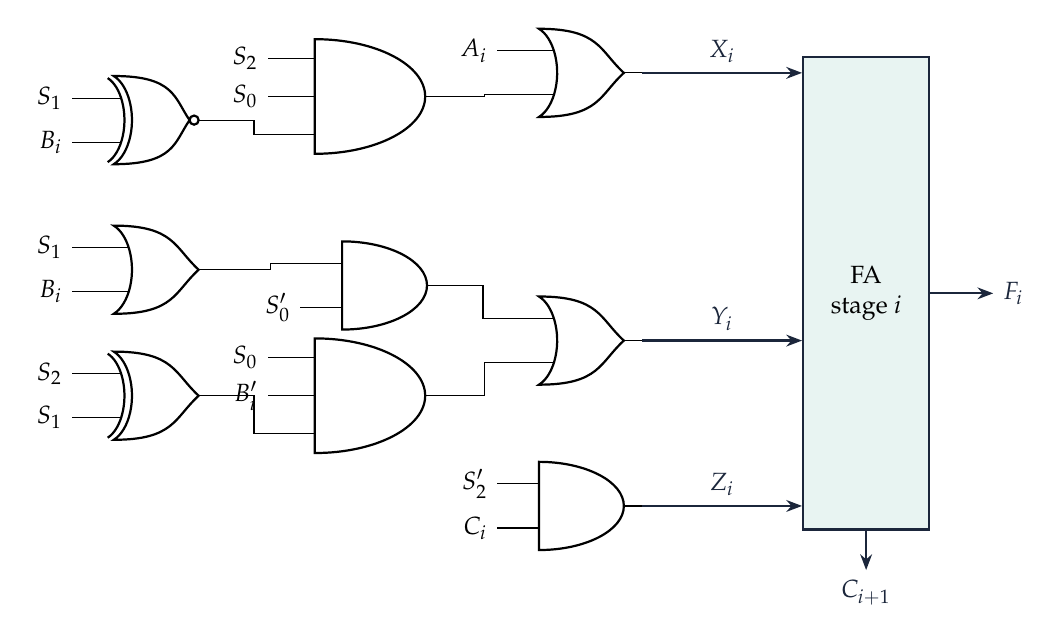
\begin{tikzpicture}[font=\small]
\node[xnor port] (g1) at (0,4) {};
\draw (g1.in 1) -- ++(-0.3,0) node[left]{$S_1$};
\draw (g1.in 2) -- ++(-0.3,0) node[left]{$B_i$};
\node[and port, number inputs=3, scale=1.3] (g2) at (2.9,4.3) {};
\draw (g2.in 1) -- ++(-0.3,0) node[left]{$S_2$};
\draw (g2.in 2) -- ++(-0.3,0) node[left]{$S_0$};
\draw (g1.out) -| ($(g1.out)!0.5!(g2.in 3)$) |- (g2.in 3);
\node[or port] (g3) at (5.4,4.6) {};
\draw (g3.in 1) -- ++(-0.3,0) node[left]{$A_i$};
\draw (g2.out) -| ($(g2.out)!0.5!(g3.in 2)$) |- (g3.in 2);
\node[or port] (g4) at (0,2.1) {};
\draw (g4.in 1) -- ++(-0.3,0) node[left]{$S_1$};
\draw (g4.in 2) -- ++(-0.3,0) node[left]{$B_i$};
\node[and port] (g5) at (2.9,1.9) {};
\draw (g4.out) -| ($(g4.out)!0.5!(g5.in 1)$) |- (g5.in 1);
\draw (g5.in 2) -- ++(-0.3,0) node[left]{$S_0'$};
\node[xor port] (g9) at (0,0.5) {};
\draw (g9.in 1) -- ++(-0.3,0) node[left]{$S_2$};
\draw (g9.in 2) -- ++(-0.3,0) node[left]{$S_1$};
\node[and port, number inputs=3, scale=1.3] (g6) at (2.9,0.5) {};
\draw (g6.in 1) -- ++(-0.3,0) node[left]{$S_0$};
\draw (g6.in 2) -- ++(-0.3,0) node[left]{$B_i'$};
\draw (g9.out) -| ($(g9.out)!0.5!(g6.in 3)$) |- (g6.in 3);
\node[or port] (g7) at (5.4,1.2) {};
\draw (g5.out) -| ($(g5.out)!0.5!(g7.in 1)$) |- (g7.in 1);
\draw (g6.out) -| ($(g6.out)!0.5!(g7.in 2)$) |- (g7.in 2);
\node[and port] (g8) at (5.4,-0.9) {};
\draw (g8.in 1) -- ++(-0.3,0) node[left]{$S_2'$};
\draw (g8.in 2) -- ++(-0.3,0) node[left]{$C_i$};
\node[blkm,minimum width=16mm,minimum height=60mm] (fa) at (8.4,1.8) {FA\\stage $i$};
\draw[wire] (g3.out) -- node[above]{$X_i$} (g3.out -| fa.west);
\draw[wire] (g7.out) -- node[above]{$Y_i$} (g7.out -| fa.west);
\draw[wire] (g8.out) -- node[above]{$Z_i$} (g8.out -| fa.west);
\draw[wire] (fa.east) -- ++(0.8,0) node[right]{$F_i$};
\draw[wire] (fa.south) -- ++(0,-0.5) node[below]{$C_{i+1}$};
\end{tikzpicture}}
{\small $S_2\oplus S_1$ is computed once and shared by all four stages. In stage 0 the $C_i$ input is tied to 0. The design was checked by simulating all $(S,A,B)$ combinations.}

\sub{(b) When is the output carry $C_{\text{out}}=1$? ($n=4$; cf.\ slide Table 9-2)}
\fig{\small\begin{tabular}{lll}\toprule
Operation (adder does) & $C_{\text{out}}=1$ when & Comment\\\midrule
Addition: $A+B$ & $A+B\ge 2^n=16$ & unsigned overflow; $F$ holds only the low 4 bits\\
Transfer $A$: $A+0+0$ & never & $C_{\text{out}}$ is always 0\\
Decrement: $A+1111$ & $A\neq0$ & $A+15\ge16 \iff A\ge1$; for $A=0$, $F=1111$, $C_{\text{out}}=0$\\
$A+B'$ ($=A-B-1$) & $A>B$ & $A+15-B\ge16\iff A>B$; else $F$ = 1's comp.\ of $(B-A)$\\\bottomrule
\end{tabular}}
\end{solution}

%===================================================================== TOPIC 04
\topic{04}{Arithmetic for Computers}

%---------------------------------------------------------------- AR01
\begin{question}{2023--2024 \textbullet\ Q7(a)}{CSE 209 \textbullet\ 29/04/2026 \textbullet\ AR01}{20}
Draw the diagram of the integer multiplication hardware following (i) long multiplication approach, and (ii) parallel add/shift approach assuming 32 bit multiplier and 32 bit multiplicand. For each approach, also simulate the steps of the multiplication with an example for two 4 bit integer numbers: 1000 (multiplicand), 1011 (multiplier).
\end{question}
\begin{solution}
\sub{(i) Long-multiplication hardware (first version)}
This copies pencil-and-paper multiplication. Each step tests Multiplier0, the multiplier's LSB. If it is 1, the multiplicand is added to the product. Then the multiplicand shifts left and the multiplier shifts right. For $32\times32$ bits this needs a 64-bit Multiplicand register (multiplicand in its right half), a 64-bit ALU, a 64-bit Product register (initially 0) and a 32-bit Multiplier register. It runs 32 iterations of up to 3 steps each.
\fig{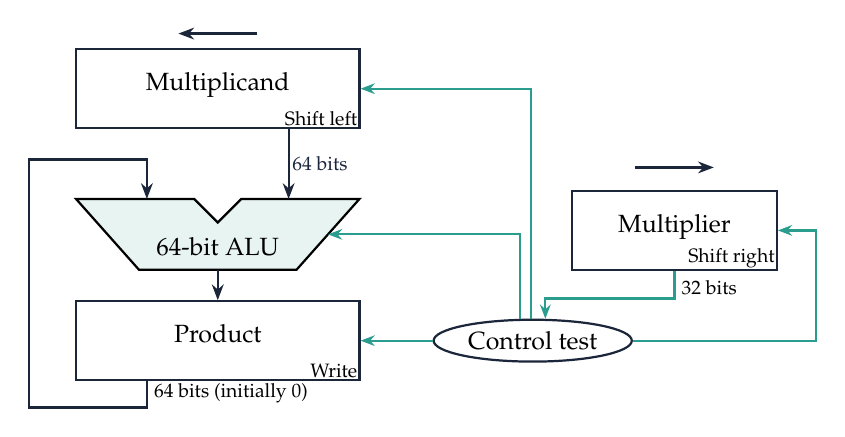
\begin{tikzpicture}[font=\small]
\node[blk,minimum width=36mm,minimum height=10mm] (mc) at (0,3) {\raisebox{5pt}{Multiplicand}};
\node[tk,anchor=south east] at (mc.south east) {Shift left};
\draw[wire] (0.5,3.7) -- (-0.5,3.7);
\draw[thick,fill=mist] (-1.8,1.6) -- (-0.3,1.6) -- (0,1.3) -- (0.3,1.6) -- (1.8,1.6) -- (1.0,0.7) -- (-1.0,0.7) -- cycle;
\node at (0,1.0) {64-bit ALU};
\draw[wire] (0.9,2.5) -- node[right,tk]{64 bits} (0.9,1.6);
\node[blk,minimum width=36mm,minimum height=10mm] (pr) at (0,-0.2) {\raisebox{5pt}{Product}};
\node[tk,anchor=south east] at (pr.south east) {Write};
\draw[wire] (0,0.7) -- (pr.north);
\draw[wire] (-0.9,-0.7) -- (-0.9,-1.05) -- (-2.4,-1.05) -- (-2.4,2.1) -- (-0.9,2.1) -- (-0.9,1.6);
\node[tk,anchor=north west] at (-0.85,-0.7) {64 bits (initially 0)};
\node[blk,minimum width=26mm,minimum height=10mm] (mp) at (5.8,1.2) {\raisebox{5pt}{Multiplier}};
\node[tk,anchor=south east] at (mp.south east) {Shift right};
\draw[wire] (5.3,2.0) -- (6.3,2.0);
\node[oval] (ct) at (4.0,-0.2) {Control test};
\node[tk,anchor=west] at (5.85,0.48) {32 bits};
\draw[ctl] (ct.west) -- (pr.east);
\draw[ctl] (ct.120) |- (1.4,1.15);
\draw[ctl] (ct.95) |- (mc.east);
\draw[ctl] (mp.south) -- ++(0,-0.35) -| (ct.60);
\draw[ctl] (ct.east) -- (7.6,-0.2) |- (mp.east);
\end{tikzpicture}}
\sub{(ii) Parallel add/shift hardware (refined version)}
The multiplicand stays still and the \emph{product shifts right}, so only a 32-bit Multiplicand register and a 32-bit ALU are needed. The ALU adds into the left half of the product. The multiplier is loaded into the right half of the 64-bit Product register, and the bit tested is Product0. The add and the shift are done in the same cycle, so the multiply takes 32 cycles.
\fig{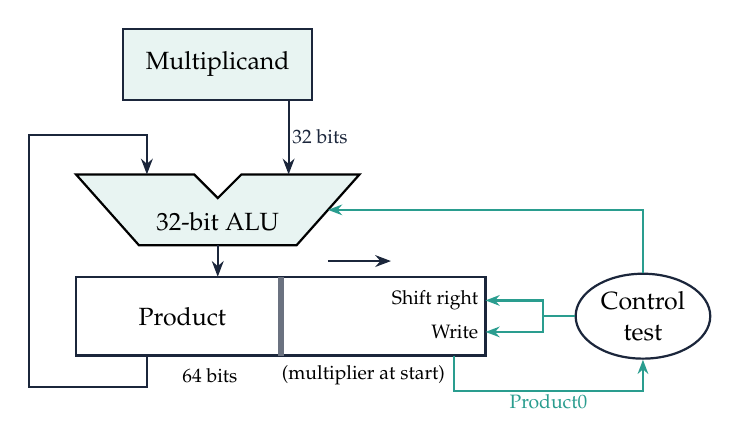
\begin{tikzpicture}[font=\small]
\node[blkm,minimum width=24mm,minimum height=9mm] (mc) at (0,3) {Multiplicand};
\draw[thick,fill=mist] (-1.8,1.6) -- (-0.3,1.6) -- (0,1.3) -- (0.3,1.6) -- (1.8,1.6) -- (1.0,0.7) -- (-1.0,0.7) -- cycle;
\node at (0,1.0) {32-bit ALU};
\draw[wire] (0.9,2.55) -- node[right,tk]{32 bits} (0.9,1.6);
\node[blk,minimum width=52mm,minimum height=10mm] (pr) at (0.8,-0.2) {};
\node at (-0.45,-0.2) {Product};
\draw[slate,line width=2pt] (0.8,-0.7) -- (0.8,0.3);
\node[tk,anchor=east] at (3.35,0.0) {Shift right};
\node[tk,anchor=east] at (3.35,-0.4) {Write};
\draw[wire] (1.4,0.5) -- (2.2,0.5);
\draw[wire] (0,0.7) -- (0,0.3);
\draw[wire] (-0.9,-0.7) -- (-0.9,-1.1) -- (-2.4,-1.1) -- (-2.4,2.1) -- (-0.9,2.1) -- (-0.9,1.6);
\node[tk] at (-0.1,-0.95) {64 bits};
\node[tk] at (1.85,-0.95) {(multiplier at start)};
\node[oval] (ct) at (5.4,-0.2) {Control\\test};
\draw[ctl] (ct.west) -- ++(-0.4,0) |- (3.4,0.0);
\draw[ctl] (ct.west) -- ++(-0.4,0) |- (3.4,-0.4);
\draw[ctl] (ct.north) |- (1.4,1.15);
\draw[ctl] (3.0,-0.7) -- (3.0,-1.15) -| node[below,tk,pos=0.25]{Product0} (ct.south);
\end{tikzpicture}}

\sub{Simulation of $1000\times1011$ \textbullet\ expected $8\times11=88=0101\,1000_2$}
Pencil-and-paper view: $1000\times1011=1000+10000+0+1000000=1011000_2$.

\textbf{(i) Long-multiplication hardware} (scaled to 4 bits: 8-bit Multiplicand and Product, 4-bit Multiplier):
\fig{\small\begin{tabular}{clccc}\toprule
Iteration & Step & Multiplier & Multiplicand & Product\\\midrule
0 & Initial values & 1011 & 0000 1000 & 0000 0000\\\midrule
1 & 1a: $1\Rightarrow$ Prod $=$ Prod $+$ Mcand & 101\textbf{1} & 0000 1000 & 0000 1000\\
  & 2: Shift left Multiplicand & 1011 & 0001 0000 & 0000 1000\\
  & 3: Shift right Multiplier & 0101 & 0001 0000 & 0000 1000\\\midrule
2 & 1a: $1\Rightarrow$ Prod $=$ Prod $+$ Mcand & 010\textbf{1} & 0001 0000 & 0001 1000\\
  & 2: Shift left Multiplicand & 0101 & 0010 0000 & 0001 1000\\
  & 3: Shift right Multiplier & 0010 & 0010 0000 & 0001 1000\\\midrule
3 & 1: $0\Rightarrow$ no operation & 001\textbf{0} & 0010 0000 & 0001 1000\\
  & 2: Shift left Multiplicand & 0010 & 0100 0000 & 0001 1000\\
  & 3: Shift right Multiplier & 0001 & 0100 0000 & 0001 1000\\\midrule
4 & 1a: $1\Rightarrow$ Prod $=$ Prod $+$ Mcand & 000\textbf{1} & 0100 0000 & 0101 1000\\
  & 2: Shift left Multiplicand & 0001 & 1000 0000 & 0101 1000\\
  & 3: Shift right Multiplier & 0000 & 1000 0000 & \textbf{0101 1000}\\\bottomrule
\end{tabular}}
\textbf{(ii) Parallel add/shift hardware} (4-bit Multiplicand, 4-bit ALU, 8-bit Product with the multiplier in its right half):
\fig{\small\begin{tabular}{clcc}\toprule
Iteration & Step & Multiplicand & Product\\\midrule
0 & Initial values (multiplier in right half) & 1000 & 0000 1011\\\midrule
1 & 1a: Prod0 $=1\Rightarrow$ left half $+=$ Mcand & 1000 & 1000 101\textbf{1}\\
  & 2: Shift right Product & 1000 & 0100 0101\\\midrule
2 & 1a: Prod0 $=1\Rightarrow$ $0100+1000$ & 1000 & 1100 010\textbf{1}\\
  & 2: Shift right Product & 1000 & 0110 0010\\\midrule
3 & 1: Prod0 $=0\Rightarrow$ no operation & 1000 & 0110 001\textbf{0}\\
  & 2: Shift right Product & 1000 & 0011 0001\\\midrule
4 & 1a: Prod0 $=1\Rightarrow$ $0011+1000$ & 1000 & 1011 000\textbf{1}\\
  & 2: Shift right Product & 1000 & \textbf{0101 1000}\\\bottomrule
\end{tabular}}
\ans{Both approaches give $1000\times1011 = 0101\,1000_2 = 88_{10}$ after 4 iterations (32 iterations for 32-bit operands). The first version needs up to 3 steps per iteration; the add/shift version needs 1 cycle per iteration.}
\end{solution}

%---------------------------------------------------------------- AR02
\repeated{4}
\begin{question}{2023--2024 \textbullet\ Q7(b)}{CSE 209 \textbullet\ 29/04/2026 \textbullet\ AR02}{15}
What is the purpose of using a positive BIAS value in IEEE 754 floating point representation? Devise the smallest and largest values that can be expressed in (i) single precision (32 bit), and (ii) double precision (64 bits) using IEEE 754 floating point representation.
\end{question}
\begin{question}{2018--2019 \textbullet\ Q7(c)}{CSE 305 \textbullet\ 29/10/2019 \textbullet\ AR02}{5}
What is the use of Bias in floating point representation? Give the encoding of the floating point ``infinity''.
\end{question}
\begin{question}{2015--2016 \textbullet\ Q7(c)}{CSE 305 \textbullet\ 18/01/2017 \textbullet\ AR02}{10}
What is the use of \emph{Bias} in floating point representation? Give the encoding of floating point \texttt{infinity}.
\end{question}
\begin{question}{2012--2013 \textbullet\ Q8(a)}{CSE 305 \textbullet\ 10/05/2014 \textbullet\ AR02}{5}
What is the purpose of using biased notation for representing exponents of floating point numbers?
\end{question}
\begin{solution}
\sub{Purpose of the bias (all four cards)}
IEEE 754 stores the exponent in \key{excess (biased) form}: stored $E$ = actual exponent + Bias, with Bias $=127$ (single, 8-bit $E$) or $1023$ (double, 11-bit $E$).
\begin{itemize}
\item \key{The exponent field is unsigned.} Negative exponents need no sign bit or 2's complement. The most negative exponent is stored as $00\ldots01$ and the most positive as $11\ldots10$.
\item \key{Fast comparison and sorting.} The layout is sign | exponent | fraction. With a biased exponent, a larger exponent is always a larger unsigned bit pattern, so two FP numbers can be compared (and sorted) with ordinary \emph{integer} compare hardware. With a 2's-complement exponent, $1.0\times2^{-1}$ (exponent \texttt{1111\,1111}) would look larger than $1.0\times2^{+1}$ (exponent \texttt{0000\,0001}). With bias 127 they are \texttt{0111\,1110} $<$ \texttt{1000\,0000}, which is correct.
\item The two end codes are left free for special values: $E=0$ for zero and denormals, $E=$ all 1s for $\pm\infty$ and NaN.
\end{itemize}
Value of a normalized number: $x=(-1)^S\times(1+\text{Fraction})\times2^{(E-\text{Bias})}$.

\sub{Smallest and largest values (2023--24 Q7(b))}
\fig{\small\begin{tabular}{@{}llll@{}}\toprule
 & Bit pattern & Value & Approx.\\\midrule
\multicolumn{4}{@{}l}{\textbf{Single} (1 + 8 + 23 bits, Bias 127)}\\
Largest & $E=1111\,1110$ ($254-127=+127$), F $=1\ldots1$ \ (\hex{7F7FFFFF}) & $(2-2^{-23})\times2^{127}$ & $3.40\times10^{38}$\\
Smallest normalized & $E=0000\,0001$ ($1-127=-126$), F $=0\ldots0$ \ (\hex{00800000}) & $1.0\times2^{-126}$ & $1.18\times10^{-38}$\\
Smallest denormal & $E=0$, F $=0\ldots01$ \ (\hex{00000001}) & $2^{-23}\times2^{-127}=2^{-150}$ & $7.0\times10^{-46}$\\\midrule
\multicolumn{4}{@{}l}{\textbf{Double} (1 + 11 + 52 bits, Bias 1023)}\\
Largest & $E=111\,1111\,1110$ ($2046-1023=+1023$), F all 1s & $(2-2^{-52})\times2^{1023}$ & $1.80\times10^{308}$\\
Smallest normalized & $E=000\,0000\,0001$ ($1-1023=-1022$), F all 0s & $1.0\times2^{-1022}$ & $2.23\times10^{-308}$\\
Smallest denormal & $E=0$, F $=0\ldots01$ & $2^{-52}\times2^{-1023}=2^{-1075}$ & $2.5\times10^{-324}$\\\bottomrule
\end{tabular}}
Denormals use the slides' formula $x=(-1)^S\times(0+\text{Fraction})\times2^{-\text{Bias}}$.
\begin{note}Real IEEE-754 hardware scales denormals by $2^{1-\text{Bias}}$ instead, so the actual hardware minimums are $2^{-149}\approx1.4\times10^{-45}$ (single) and $2^{-1074}\approx4.9\times10^{-324}$ (double). The table follows the course slides.\end{note}

The sign bit is separate, so each range is symmetric. The most negative values are $-(2-2^{-23})\times2^{127}\approx-3.4\times10^{38}$ (single) and $-(2-2^{-52})\times2^{1023}\approx-1.8\times10^{308}$ (double).
\ans{Single: $\pm1.0\times2^{-126}\approx\pm1.2\times10^{-38}$ to $\pm(2-2^{-23})\times2^{127}\approx\pm3.4\times10^{38}$. \ Double: $\pm1.0\times2^{-1022}\approx\pm2.2\times10^{-308}$ to $\pm(2-2^{-52})\times2^{1023}\approx\pm1.8\times10^{308}$.}

\sub{Encoding of infinity (2018--19 Q7(c), 2015--16 Q7(c))}
Infinity is \key{exponent all 1s, fraction all 0s}. The sign bit tells $+\infty$ from $-\infty$. If the exponent is all 1s and the fraction is \emph{not} zero, the value is NaN (e.g.\ $0/0$).
\fig{\small\begin{tabular}{lccl}\toprule
 & S & Exponent & Fraction \quad(hex)\\\midrule
$+\infty$ (single) & 0 & 1111\,1111 & 000\ldots0 \quad(\hex{7F800000})\\
$-\infty$ (single) & 1 & 1111\,1111 & 000\ldots0 \quad(\hex{FF800000})\\
$+\infty$ (double) & 0 & 111\,1111\,1111 & 000\ldots0 \quad(\hex{7FF0000000000000})\\\bottomrule
\end{tabular}}
$\pm\infty$ is produced on overflow (e.g.\ $1/0$). It can be used in later calculations without a separate overflow check.
\end{solution}

%---------------------------------------------------------------- AR03
\repeated{5}
\begin{question}{2022--2023 \textbullet\ Q1(a)}{CSE 209 \textbullet\ 13/01/2025 \textbullet\ AR03}{10}
Express the steps of floating-point addition using a flow chart. Also, write down the conditions of overflow, underflow, NaN and infinity during a floating-point addition.
\end{question}
\begin{question}{2018--2019 \textbullet\ Q8(b)}{CSE 305 \textbullet\ 29/10/2019 \textbullet\ AR03}{10}
What are the steps of floating point addition? Describe with an example. Also, write down the condition of overflow and underflow during a floating point addition.
\end{question}
\begin{question}{2015--2016 \textbullet\ Q6(a)}{CSE 305 \textbullet\ 18/01/2017 \textbullet\ AR03}{12}
What are the steps of floating point addition? Describe with an example.
\end{question}
\begin{question}{2013--2014 \textbullet\ Q3(a)}{CSE 305 \textbullet\ 05/07/2015 \textbullet\ AR03}{10}
Write down the steps for the addition of two binary floating point numbers.
\end{question}
\begin{question}{2011--2012 \textbullet\ Q5(a)}{CSE 305 \textbullet\ 27/07/2013 \textbullet\ AR03}{8 + 2}
Draw the flow diagram of floating point addition. Also write down the condition of overflow or underflow during a floating point addition.
\end{question}
\begin{solution}
\sub{Steps / flow chart of FP addition (all cards)}
For $x = (-1)^{s_x}\,1.f_x\times 2^{e_x}$ and $y = (-1)^{s_y}\,1.f_y\times 2^{e_y}$:
\begin{enumerate}[label=\textbf{\arabic*.}]
\item \key{Align}: compare exponents (small ALU computes $e_x-e_y$); shift the significand of the number with the \emph{smaller} exponent right by $|e_x-e_y|$ places; the result takes the larger exponent.
\item \key{Add} the (signed) significands in the big ALU.
\item \key{Normalize}: shift the sum right and increment the exponent, or shift left and decrement it, until it is $1.xxx$; then \key{check for overflow/underflow}.
\item \key{Round} the significand to the available bits (using guard/round/sticky); if rounding de-normalizes it (e.g.\ $1.111\to10.000$), go back to step 3.
\end{enumerate}
\fig{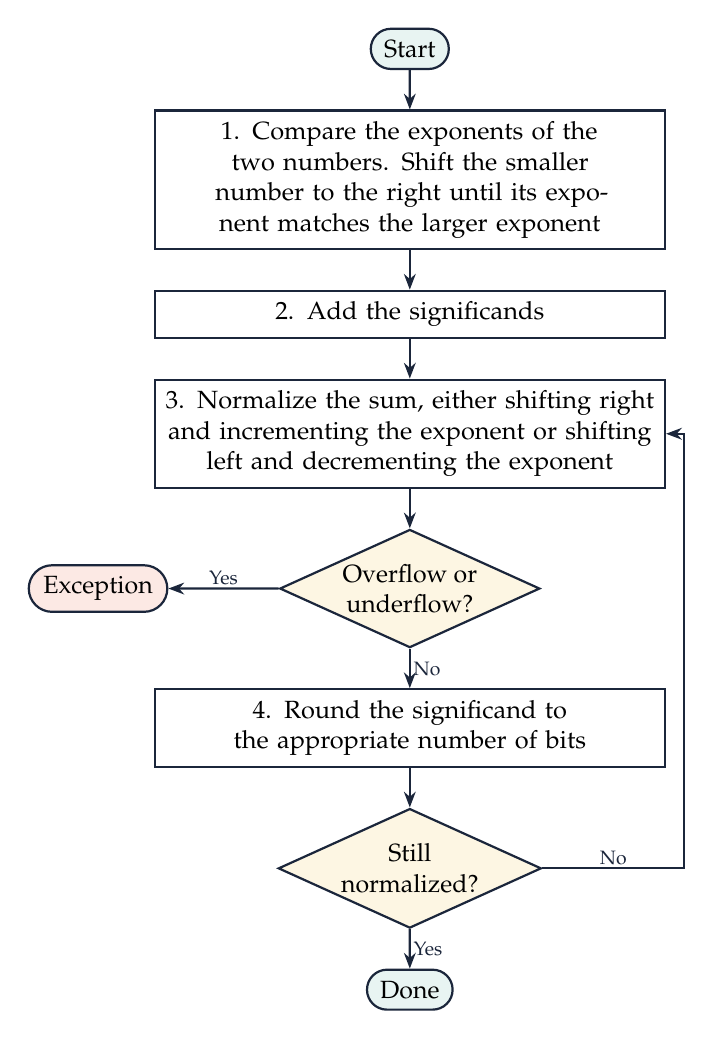
\begin{tikzpicture}[node distance=5mm]
\node[term] (s) {Start};
\node[proc,below=of s,text width=62mm] (p1) {1. Compare the exponents of the two numbers. Shift the smaller number to the right until its exponent matches the larger exponent};
\node[proc,below=of p1,text width=62mm] (p2) {2. Add the significands};
\node[proc,below=of p2,text width=62mm] (p3) {3. Normalize the sum, either shifting right and incrementing the exponent or shifting left and decrementing the exponent};
\node[dec,below=of p3] (d1) {Overflow or\\underflow?};
\node[term,fill=rose,left=14mm of d1] (ex) {Exception};
\node[proc,below=of d1,text width=62mm] (p4) {4. Round the significand to the appropriate number of bits};
\node[dec,below=of p4] (d2) {Still\\normalized?};
\node[term,below=of d2] (dn) {Done};
\draw[wire] (s)--(p1); \draw[wire] (p1)--(p2); \draw[wire] (p2)--(p3); \draw[wire] (p3)--(d1);
\draw[wire] (d1)--node[tk,above]{Yes}(ex);
\draw[wire] (d1)--node[tk,right]{No}(p4);
\draw[wire] (p4)--(d2);
\draw[wire] (d2)--node[tk,right]{Yes}(dn);
\draw[wire] (d2.east)--node[tk,above]{No}++(18mm,0) |- (p3.east);
\end{tikzpicture}}

\sub{Example (2018--19 Q8(b), 2015--16 Q6(a)) --- 4-bit significands: $0.5 + (-0.4375)$}
{\small\begin{tabular}{@{}ll@{}}
Operands & $1.000_2\times2^{-1}$ \ and \ $-1.110_2\times2^{-2}$\\
1. Align (shift smaller right by 1) & $1.000\times2^{-1} + (-0.111\times2^{-1})$\\
2. Add significands & $1.000-0.111 = 0.001\times2^{-1}$\\
3. Normalize (shift left 3, exponent $-1-3$) & $1.000\times2^{-4}$; $-126\le -4\le 127$ $\Rightarrow$ no over/underflow\\
4. Round & $1.000\times2^{-4}$ (no change) $= 0.0625$ \ok
\end{tabular}}

\sub{Exception conditions (IEEE single; biased exponent $E$, 1\,..\,254 for normal numbers)}
\begin{itemize}
\item \key{Overflow}: after normalization (right shift, exponent incremented) the exponent exceeds the largest value, i.e.\ $E > 254$ (true exponent $>+127$; double: $>+1023$). Result is set to $\pm\infty$.
\item \key{Underflow}: after normalization (left shift, exponent decremented) the exponent falls below the smallest value, i.e.\ $E < 1$ (true exponent $<-126$; double: $<-1022$). Result becomes a denormal or $0$.
\item \key{NaN} (2022--23 card): either operand is a NaN ($E=255$, $F\ne0$), or the operation is $(+\infty)+(-\infty)$ (invalid). Result: NaN.
\item \key{Infinity} (2022--23 card): an operand is $\pm\infty$ ($E=255$, $F=0$) and the other is finite or the same-signed $\infty$ $\Rightarrow$ result is that $\infty$; also produced by overflow.
\end{itemize}
\end{solution}

%---------------------------------------------------------------- AR04
\begin{question}{2022--2023 \textbullet\ Q1(b)}{CSE 209 \textbullet\ 13/01/2025 \textbullet\ AR04}{10}
Suppose you have a 6-bit ALU and you are required to perform a division operation, where the dividend is \texttt{1011 1100 1111} and the divisor is \texttt{110101}. Determine the result of the division process; show the step-by-step calculation along with the value of each relevant register at each step.
\end{question}
\begin{solution}
\sub{Hardware: the Optimized Divider (slides)}
With a 6-bit ALU, $n=6$: the \textbf{Divisor} register is 6 bits and the \textbf{Remainder} register is $2n=12$ bits. There is no separate Quotient register. The ALU works on the left half Rem$_{hi}$ and the Divisor, and the quotient bits are shifted in from the right end of the Remainder.
\fig{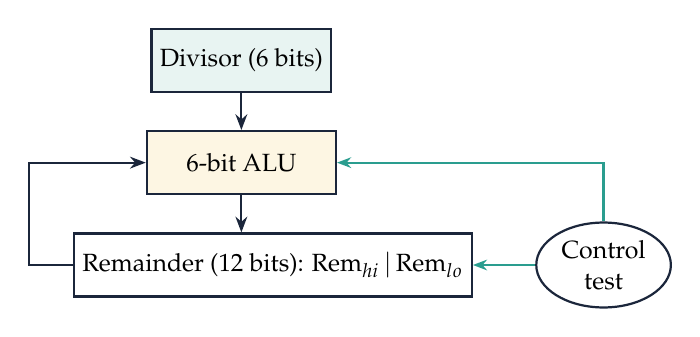
\begin{tikzpicture}[font=\small]
 \node[blkm,minimum width=20mm] (dv) at (0,0) {Divisor (6 bits)};
 \node[blkg,minimum width=24mm] (al) at (0,-1.3) {6-bit ALU};
 \node[blk,minimum width=48mm] (rm) at (0.4,-2.6) {Remainder (12 bits): Rem$_{hi}$\,$|$\,Rem$_{lo}$};
 \node[oval] (ct) at (4.6,-2.6) {Control\\test};
 \draw[wire] (dv) -- (al);
 \draw[wire] (al) -- ($(rm.north)+(-0.4,0)$);
 \draw[wire] ($(rm.west)$) -| (-2.7,-1.3) -- (al.west);
 \draw[ctl] (ct.west) -- (rm.east);
 \draw[ctl] (ct.north) |- (al.east);
\end{tikzpicture}}
\textbf{Algorithm (slides).} \textbf{0.}~Remainder $\leftarrow$ dividend, then shift Remainder left 1.
Repeat $n=6$ times: \textbf{1.}~Rem$_{hi}\leftarrow$ Rem$_{hi}-$Divisor; \textbf{2a.}~if Rem$_{hi}\ge0$: shift Remainder left, new rightmost bit $=1$; \textbf{2b.}~if Rem$_{hi}<0$: restore (Rem$_{hi}\leftarrow$ Rem$_{hi}+$Divisor), shift Remainder left, new rightmost bit $=0$. \textbf{3.}~Finally shift Rem$_{hi}$ right 1. Then Rem$_{hi}=$ remainder and Rem$_{lo}=$ quotient.

\textbf{Why shift first?} The first quotient bit has weight $2^{n-1}$: it asks whether Divisor$\times2^{n-1}$ fits, i.e.\ it compares the Divisor with the dividend's top $n{+}1$ bits, which is what the left half holds after one left shift. Subtracting from the unshifted left half would test Divisor$\times2^{n}$, a quotient bit an $n$-bit quotient cannot have (it always fails for a valid division). The extra left shift is undone by the final right shift of Rem$_{hi}$.

\begin{note}The dividend's leading bit is 1, so the first left shift pushes a bit out of the 6-bit left half. The ALU must keep that bit (as its carry/7th bit), otherwise the dividend would be corrupted. In the table Rem$_{hi}$ is therefore shown with this extra leading bit (7 bits). Negative differences are in 2's complement. Values that change are in \textcolor{coral}{\textbf{coral}}.\end{note}

\sub{Trace: $\texttt{101111001111}_2 \div \texttt{110101}_2$ \ ($3023 \div 53$)}
\fig{\footnotesize\setlength{\tabcolsep}{4pt}\begin{tabular}{c>{\raggedright\arraybackslash}p{50mm}ccc}
\toprule
Iter. & Step & Divisor & Remainder (Rem$_{hi}$\,$|$\,Rem$_{lo}$) & sign\\
\midrule
0 & Initial values & \texttt{110101} & \texttt{0101111}\,$|$\,\texttt{001111} & \\
 & Shift Rem left 1 & \texttt{110101} & \textcolor{coral}{\textbf{\texttt{1011110}}}\,$|$\,\textcolor{coral}{\textbf{\texttt{011110}}} & \\
\midrule
1 & 1: Rem$_{hi}$ $\leftarrow$ Rem$_{hi}-$Div & \texttt{110101} & \textcolor{coral}{\textbf{\texttt{0101001}}}\,$|$\,\texttt{011110} & $\ge 0$\\
 & 2a: Rem$\ge$0: sll Rem, Rem$_0{=}1$ & \texttt{110101} & \textcolor{coral}{\textbf{\texttt{1010010}}}\,$|$\,\textcolor{coral}{\textbf{\texttt{111101}}} & \\
\midrule
2 & 1: Rem$_{hi}$ $\leftarrow$ Rem$_{hi}-$Div & \texttt{110101} & \textcolor{coral}{\textbf{\texttt{0011101}}}\,$|$\,\texttt{111101} & $\ge 0$\\
 & 2a: Rem$\ge$0: sll Rem, Rem$_0{=}1$ & \texttt{110101} & \textcolor{coral}{\textbf{\texttt{0111011}}}\,$|$\,\textcolor{coral}{\textbf{\texttt{111011}}} & \\
\midrule
3 & 1: Rem$_{hi}$ $\leftarrow$ Rem$_{hi}-$Div & \texttt{110101} & \textcolor{coral}{\textbf{\texttt{0000110}}}\,$|$\,\texttt{111011} & $\ge 0$\\
 & 2a: Rem$\ge$0: sll Rem, Rem$_0{=}1$ & \texttt{110101} & \textcolor{coral}{\textbf{\texttt{0001101}}}\,$|$\,\textcolor{coral}{\textbf{\texttt{110111}}} & \\
\bottomrule
\end{tabular}}
\fig{\footnotesize\setlength{\tabcolsep}{4pt}\begin{tabular}{c>{\raggedright\arraybackslash}p{50mm}ccc}
\toprule
Iter. & Step & Divisor & Remainder (Rem$_{hi}$\,$|$\,Rem$_{lo}$) & sign \ \textit{(cont.)}\\
\midrule
4 & 1: Rem$_{hi}$ $\leftarrow$ Rem$_{hi}-$Div & \texttt{110101} & \textcolor{coral}{\textbf{\texttt{1011000}}}\,$|$\,\texttt{110111} & $<0$\\
 & 2b: Rem$<$0: $+$Div, sll Rem, Rem$_0{=}0$ & \texttt{110101} & \textcolor{coral}{\textbf{\texttt{0011011}}}\,$|$\,\textcolor{coral}{\textbf{\texttt{101110}}} & \\
\midrule
5 & 1: Rem$_{hi}$ $\leftarrow$ Rem$_{hi}-$Div & \texttt{110101} & \textcolor{coral}{\textbf{\texttt{1100110}}}\,$|$\,\texttt{101110} & $<0$\\
 & 2b: Rem$<$0: $+$Div, sll Rem, Rem$_0{=}0$ & \texttt{110101} & \textcolor{coral}{\textbf{\texttt{0110111}}}\,$|$\,\textcolor{coral}{\textbf{\texttt{011100}}} & \\
\midrule
6 & 1: Rem$_{hi}$ $\leftarrow$ Rem$_{hi}-$Div & \texttt{110101} & \textcolor{coral}{\textbf{\texttt{0000010}}}\,$|$\,\texttt{011100} & $\ge 0$\\
 & 2a: Rem$\ge$0: sll Rem, Rem$_0{=}1$ & \texttt{110101} & \textcolor{coral}{\textbf{\texttt{0000100}}}\,$|$\,\textcolor{coral}{\textbf{\texttt{111001}}} & \\
\midrule
 & 3: Shift Rem$_{hi}$ right 1 & \texttt{110101} & \textcolor{coral}{\textbf{\texttt{0000010}}}\,$|$\,\texttt{111001} & \\
\bottomrule
\end{tabular}}
\ans{Quotient $=$ Rem$_{lo}=\texttt{111001}_2 = 57$, Remainder $=$ Rem$_{hi}=\texttt{000010}_2 = 2$. \ Check: $53\times57+2 = 3023$ \ok}
\end{solution}

%---------------------------------------------------------------- AR05
\repeated{6}
\begin{question}{2022--2023 \textbullet\ Q4}{CSE 209 \textbullet\ 13/01/2025 \textbullet\ AR05}{15}
Draw the hardware block diagram and the flowchart of the sequential version of the multiplication algorithm. Also, draw the hardware block diagram and the flowchart of the refined version of the algorithm.
\end{question}
\begin{question}{2019--2020 \textbullet\ Q4(b)}{CSE 305 \textbullet\ 18/09/2021 \textbullet\ AR05}{12}
See the diagram (Figure 4b) of the following multiplication hardware.
\fig{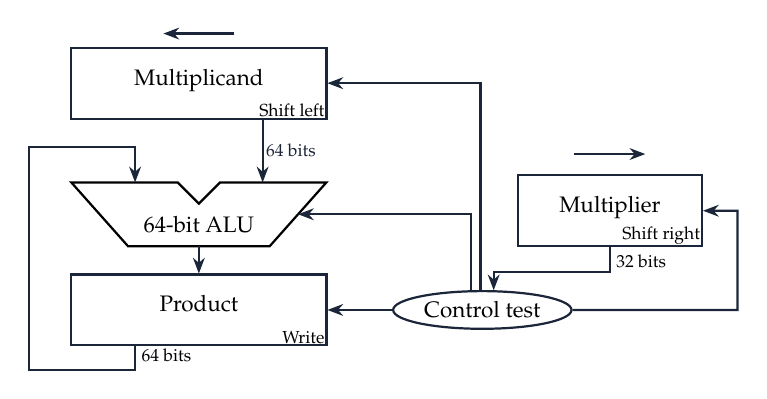
\begin{tikzpicture}[font=\small,scale=0.9,transform shape]
\node[blk,minimum width=36mm,minimum height=10mm] (mc) at (0,3) {\raisebox{5pt}{Multiplicand}};
\node[tk,anchor=south east] at (mc.south east) {Shift left};
\draw[wire] (0.5,3.7) -- (-0.5,3.7);
\draw[thick,fill=white] (-1.8,1.6) -- (-0.3,1.6) -- (0,1.3) -- (0.3,1.6) -- (1.8,1.6) -- (1.0,0.7) -- (-1.0,0.7) -- cycle;
\node at (0,1.0) {64-bit ALU};
\draw[wire] (0.9,2.5) -- node[right,tk]{64 bits} (0.9,1.6);
\node[blk,minimum width=36mm,minimum height=10mm] (pr) at (0,-0.2) {\raisebox{5pt}{Product}};
\node[tk,anchor=south east] at (pr.south east) {Write};
\draw[wire] (0,0.7) -- (pr.north);
\draw[wire] (-0.9,-0.7) -- (-0.9,-1.05) -- (-2.4,-1.05) -- (-2.4,2.1) -- (-0.9,2.1) -- (-0.9,1.6);
\node[tk,anchor=north west] at (-0.85,-0.7) {64 bits};
\node[blk,minimum width=26mm,minimum height=10mm] (mp) at (5.8,1.2) {\raisebox{5pt}{Multiplier}};
\node[tk,anchor=south east] at (mp.south east) {Shift right};
\draw[wire] (5.3,2.0) -- (6.3,2.0);
\node[oval] (ct) at (4.0,-0.2) {Control test};
\node[tk,anchor=west] at (5.85,0.48) {32 bits};
\draw[wire] (ct.west) -- (pr.east);
\draw[wire] (ct.120) |- (1.4,1.15);
\draw[wire] (ct.95) |- (mc.east);
\draw[wire] (mp.south) -- ++(0,-0.35) -| (ct.60);
\draw[wire] (ct.east) -- (7.6,-0.2) |- (mp.east);
\end{tikzpicture}}
\begin{center}\small\textbf{Figure 4b: Multiplication Hardware}\end{center}
Briefly describe the reasons why this hardware is inefficient for a multiplication operation. What changes are required to make this hardware efficient? Draw the diagram of the efficient hardware.
\end{question}
\begin{question}{2018--2019 \textbullet\ Q5(a)}{CSE 305 \textbullet\ 29/10/2019 \textbullet\ AR05}{12}
Draw the hardware block diagram and the flowchart of the sequential version of the multiplication algorithm. Also, draw the flowchart of the refined version of the algorithm.
\end{question}
\begin{question}{2014--2015 \textbullet\ Q8(b)}{CSE 305 \textbullet\ 26/01/2016 \textbullet\ AR05}{8 + 5}
In the following figure, a multiplication hardware is given. Now draw the flowchart of a the sequential version of multiplication algorithm for this hardware. Please note that, this simple hardware is not register-optimized, therefore, draw a register-optimized refined version of this hardware.
\fig{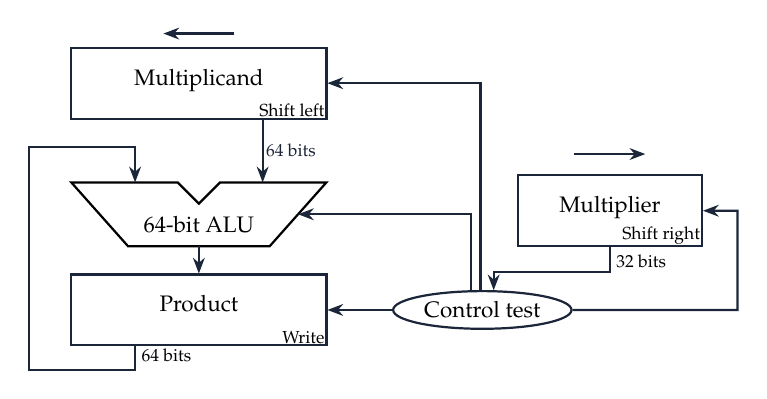
\begin{tikzpicture}[font=\small,scale=0.9,transform shape]
\node[blk,minimum width=36mm,minimum height=10mm] (mc) at (0,3) {\raisebox{5pt}{Multiplicand}};
\node[tk,anchor=south east] at (mc.south east) {Shift left};
\draw[wire] (0.5,3.7) -- (-0.5,3.7);
\draw[thick,fill=white] (-1.8,1.6) -- (-0.3,1.6) -- (0,1.3) -- (0.3,1.6) -- (1.8,1.6) -- (1.0,0.7) -- (-1.0,0.7) -- cycle;
\node at (0,1.0) {64-bit ALU};
\draw[wire] (0.9,2.5) -- node[right,tk]{64 bits} (0.9,1.6);
\node[blk,minimum width=36mm,minimum height=10mm] (pr) at (0,-0.2) {\raisebox{5pt}{Product}};
\node[tk,anchor=south east] at (pr.south east) {Write};
\draw[wire] (0,0.7) -- (pr.north);
\draw[wire] (-0.9,-0.7) -- (-0.9,-1.05) -- (-2.4,-1.05) -- (-2.4,2.1) -- (-0.9,2.1) -- (-0.9,1.6);
\node[tk,anchor=north west] at (-0.85,-0.7) {64 bits};
\node[blk,minimum width=26mm,minimum height=10mm] (mp) at (5.8,1.2) {\raisebox{5pt}{Multiplier}};
\node[tk,anchor=south east] at (mp.south east) {Shift right};
\draw[wire] (5.3,2.0) -- (6.3,2.0);
\node[oval] (ct) at (4.0,-0.2) {Control test};
\node[tk,anchor=west] at (5.85,0.48) {32 bits};
\draw[wire] (ct.west) -- (pr.east);
\draw[wire] (ct.120) |- (1.4,1.15);
\draw[wire] (ct.95) |- (mc.east);
\draw[wire] (mp.south) -- ++(0,-0.35) -| (ct.60);
\draw[wire] (ct.east) -- (7.6,-0.2) |- (mp.east);
\end{tikzpicture}}
\end{question}
\begin{question}{2013--2014 \textbullet\ Q3(c)}{CSE 305 \textbullet\ 05/07/2015 \textbullet\ AR05}{15}
Draw a block diagram of hardware organization and corresponding flowchart for the multiplication of two 32-bit binary unsigned integer numbers, where there is no separate multiplier register.
\end{question}
\begin{question}{2011--2012 \textbullet\ Q6(a)}{CSE 305 \textbullet\ 27/07/2013 \textbullet\ AR05}{15}
Draw diagrams of the first and refined versions of the multiplication hardware. Discuss the improvement of the refined version over the first version.
\end{question}
\begin{solution}
\sub{1. First (sequential) version \textbullet\ hardware + flowchart (Figure 4b is exactly this hardware)}
This copies pencil-and-paper multiplication. The multiplicand shifts left one place per step. The multiplier shifts right, so the bit to test is always Multiplier0, and a partial product is added only when that bit is 1. For $32\times32$ bits the hardware is:
\begin{itemize}
\item a 64-bit Multiplicand register (right half initially holds the multiplicand, left half 0);
\item a 64-bit ALU;
\item a 64-bit Product register (initially 0);
\item a 32-bit Multiplier register.
\end{itemize}
\fig{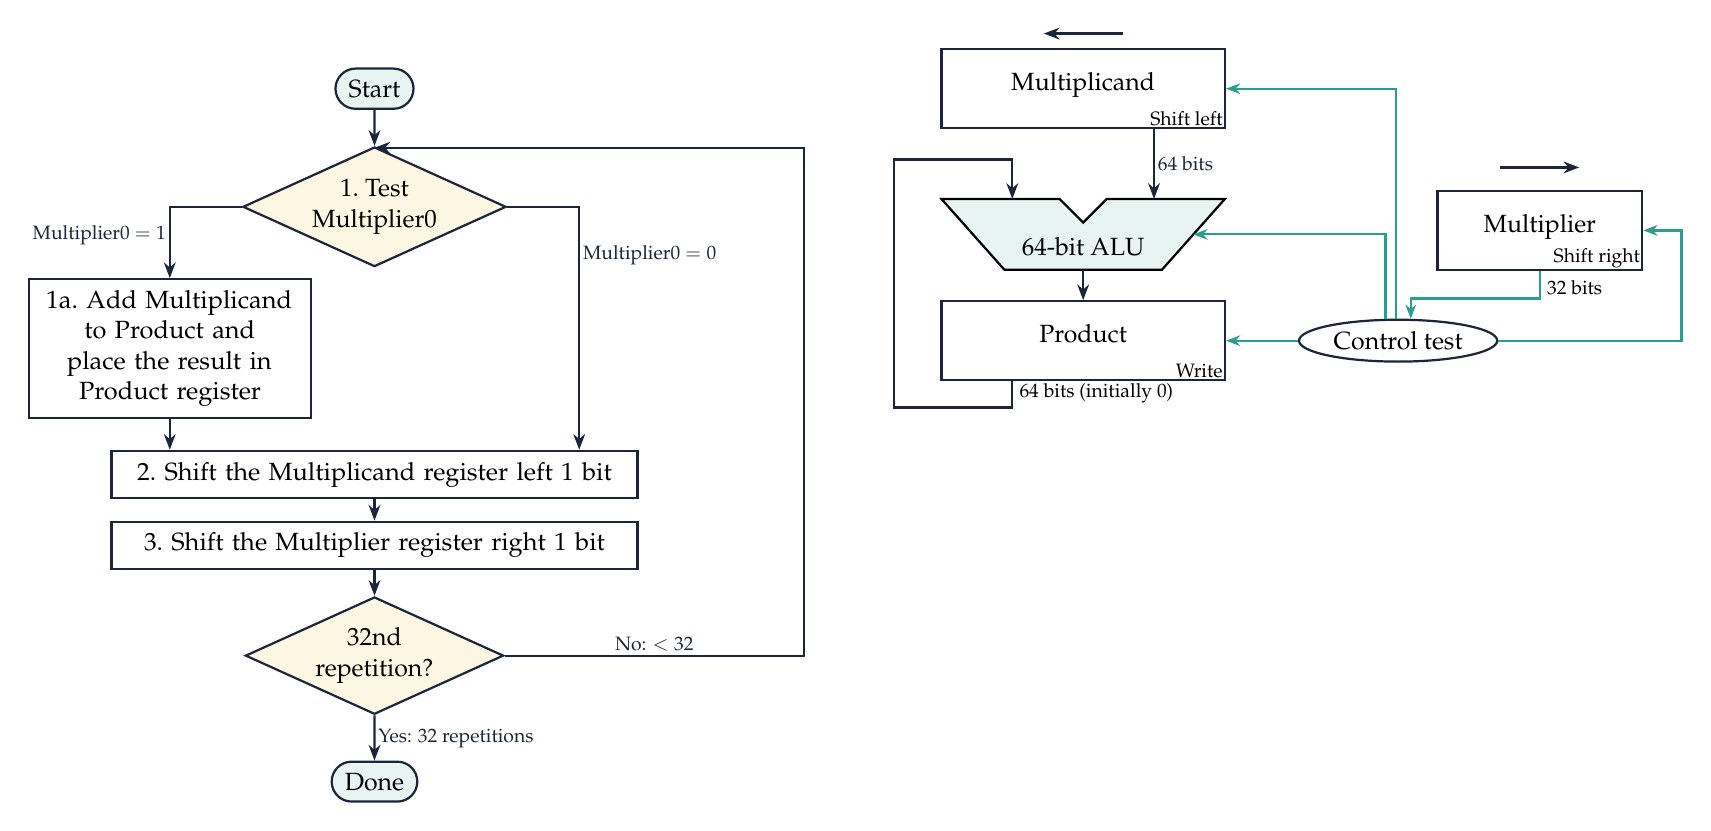
\begin{tikzpicture}[font=\small]
\begin{scope}
\node[term] (s) at (0,0) {Start};
\node[dec] (t) at (0,-1.5) {1.\ Test\\Multiplier0};
\node[proc,text width=33mm] (a) at (-2.6,-3.3) {1a.\ Add Multiplicand to Product and place the result in Product register};
\node[proc,text width=64mm] (p2) at (0,-4.9) {2.\ Shift the Multiplicand register left 1 bit};
\node[proc,text width=64mm] (p3) at (0,-5.8) {3.\ Shift the Multiplier register right 1 bit};
\node[dec] (r) at (0,-7.2) {32nd\\repetition?};
\node[term] (d) at (0,-8.8) {Done};
\draw[wire] (s) -- (t);
\draw[wire] (t.west) -| node[left,tk,pos=0.7]{Multiplier0 $=1$} (a.north);
\draw[wire] (a.south) -- (a.south |- p2.north);
\draw[wire] (t.east) -| node[right,tk,pos=0.6]{Multiplier0 $=0$} ($(p2.north)+(2.6,0)$);
\draw[wire] (p2) -- (p3);
\draw[wire] (p3) -- (r);
\draw[wire] (r.south) -- node[right,tk]{Yes: 32 repetitions} (d);
\draw[wire] (r.east) -- ++(3.8,0) node[above,tk,pos=0.5]{No: $<32$} |- (0,-0.75);
\end{scope}
\begin{scope}[xshift=9cm,yshift=-3cm]
\node[blk,minimum width=36mm,minimum height=10mm] (mc) at (0,3) {\raisebox{5pt}{Multiplicand}};
\node[tk,anchor=south east] at (mc.south east) {Shift left};
\draw[wire] (0.5,3.7) -- (-0.5,3.7);
\draw[thick,fill=mist] (-1.8,1.6) -- (-0.3,1.6) -- (0,1.3) -- (0.3,1.6) -- (1.8,1.6) -- (1.0,0.7) -- (-1.0,0.7) -- cycle;
\node at (0,1.0) {64-bit ALU};
\draw[wire] (0.9,2.5) -- node[right,tk]{64 bits} (0.9,1.6);
\node[blk,minimum width=36mm,minimum height=10mm] (pr) at (0,-0.2) {\raisebox{5pt}{Product}};
\node[tk,anchor=south east] at (pr.south east) {Write};
\draw[wire] (0,0.7) -- (pr.north);
\draw[wire] (-0.9,-0.7) -- (-0.9,-1.05) -- (-2.4,-1.05) -- (-2.4,2.1) -- (-0.9,2.1) -- (-0.9,1.6);
\node[tk,anchor=north west] at (-0.85,-0.7) {64 bits (initially 0)};
\node[blk,minimum width=26mm,minimum height=10mm] (mp) at (5.8,1.2) {\raisebox{5pt}{Multiplier}};
\node[tk,anchor=south east] at (mp.south east) {Shift right};
\draw[wire] (5.3,2.0) -- (6.3,2.0);
\node[oval] (ct) at (4.0,-0.2) {Control test};
\node[tk,anchor=west] at (5.85,0.48) {32 bits};
\draw[ctl] (ct.west) -- (pr.east);
\draw[ctl] (ct.120) |- (1.4,1.15);
\draw[ctl] (ct.95) |- (mc.east);
\draw[ctl] (mp.south) -- ++(0,-0.35) -| (ct.60);
\draw[ctl] (ct.east) -- (7.6,-0.2) |- (mp.east);
\end{scope}
\end{tikzpicture}}

\sub{2. Refined (register-optimized) version \textbullet\ hardware + flowchart}
The multiplicand stays still and the \emph{product shifts right} instead. Only 32 bits are added in each step, so the ALU and the Multiplicand register shrink to 32 bits. The multiplier starts in the right half of the 64-bit Product register, so \key{there is no separate Multiplier register}; this is the design asked for in 2013--14 Q3(c). The bit tested is Product0. The ALU writes the left half, and its carry-out enters the MSB on the shift. Add and shift happen in the same clock cycle, so each iteration takes one cycle.
\fig{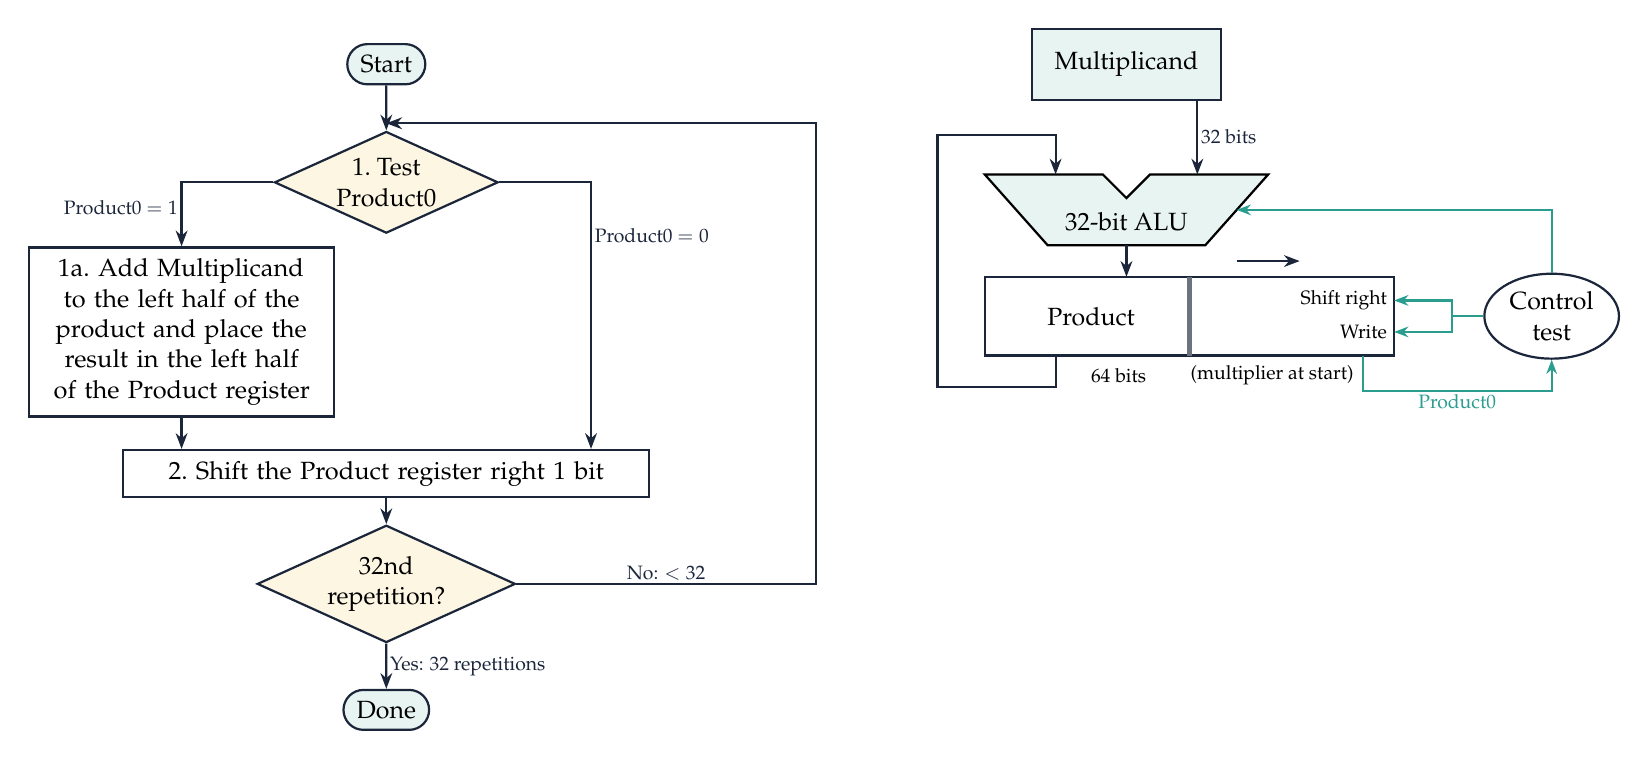
\begin{tikzpicture}[font=\small]
\begin{scope}
\node[term] (s) at (0,0) {Start};
\node[dec] (t) at (0,-1.5) {1.\ Test\\Product0};
\node[proc,text width=36mm] (a) at (-2.6,-3.4) {1a.\ Add Multiplicand to the left half of the product and place the result in the left half of the Product register};
\node[proc,text width=64mm] (p2) at (0,-5.2) {2.\ Shift the Product register right 1 bit};
\node[dec] (r) at (0,-6.6) {32nd\\repetition?};
\node[term] (d) at (0,-8.2) {Done};
\draw[wire] (s) -- (t);
\draw[wire] (t.west) -| node[left,tk,pos=0.7]{Product0 $=1$} (a.north);
\draw[wire] (a.south) -- (a.south |- p2.north);
\draw[wire] (t.east) -| node[right,tk,pos=0.6]{Product0 $=0$} ($(p2.north)+(2.6,0)$);
\draw[wire] (p2) -- (r);
\draw[wire] (r.south) -- node[right,tk]{Yes: 32 repetitions} (d);
\draw[wire] (r.east) -- ++(3.8,0) node[above,tk,pos=0.5]{No: $<32$} |- (0,-0.75);
\end{scope}
\begin{scope}[xshift=9.4cm,yshift=-3cm]
\node[blkm,minimum width=24mm,minimum height=9mm] (mc) at (0,3) {Multiplicand};
\draw[thick,fill=mist] (-1.8,1.6) -- (-0.3,1.6) -- (0,1.3) -- (0.3,1.6) -- (1.8,1.6) -- (1.0,0.7) -- (-1.0,0.7) -- cycle;
\node at (0,1.0) {32-bit ALU};
\draw[wire] (0.9,2.55) -- node[right,tk]{32 bits} (0.9,1.6);
\node[blk,minimum width=52mm,minimum height=10mm] (pr) at (0.8,-0.2) {};
\node at (-0.45,-0.2) {Product};
\draw[slate,line width=2pt] (0.8,-0.7) -- (0.8,0.3);
\node[tk,anchor=east] at (3.35,0.0) {Shift right};
\node[tk,anchor=east] at (3.35,-0.4) {Write};
\draw[wire] (1.4,0.5) -- (2.2,0.5);
\draw[wire] (0,0.7) -- (0,0.3);
\draw[wire] (-0.9,-0.7) -- (-0.9,-1.1) -- (-2.4,-1.1) -- (-2.4,2.1) -- (-0.9,2.1) -- (-0.9,1.6);
\node[tk] at (-0.1,-0.95) {64 bits};
\node[tk] at (1.85,-0.95) {(multiplier at start)};
\node[oval] (ct) at (5.4,-0.2) {Control\\test};
\draw[ctl] (ct.west) -- ++(-0.4,0) |- (3.4,0.0);
\draw[ctl] (ct.west) -- ++(-0.4,0) |- (3.4,-0.4);
\draw[ctl] (ct.north) |- (1.4,1.15);
\draw[ctl] (3.0,-0.7) -- (3.0,-1.15) -| node[below,tk,pos=0.25]{Product0} (ct.south);
\end{scope}
\end{tikzpicture}}

\sub{3. Why the first version is inefficient, and the improvement (2019--20 Q4(b), 2011--12 Q6(a), 2014--15 Q8(b))}
\begin{tabular}{@{}p{0.47\linewidth}p{0.49\linewidth}@{}}
\textbf{Inefficiencies of the first version (Figure 4b)} & \textbf{Changes in the refined hardware}\\\midrule
At any moment half of the 64-bit Multiplicand register holds only 0s. & The Multiplicand register is 32 bits and is never shifted.\\
The 64-bit ALU is twice as wide as needed. Each addition really involves only 32 significant bits, because the low product bits are already final. & The product is shifted right instead, so a \key{32-bit ALU} adds into the left half only.\\
A separate 32-bit Multiplier register is used, while the right half of the Product register is empty at the start. & The multiplier is loaded into the \key{right half of the Product register}. It is consumed bit by bit as the product shifts in, so one register is saved.\\
Each iteration takes up to 3 steps (add, shift left, shift right), about $3\times32\approx 96$ cycles in all. & Add and shift are done \key{in parallel}: one cycle per iteration, 32 cycles in total.\\
\end{tabular}
\end{solution}

%---------------------------------------------------------------- AR06
\repeated{2}
\begin{question}{2022--2023 \textbullet\ Q8(a)}{CSE 305 \textbullet\ 25/04/2024 \textbullet\ AR06}{7}
Write down equivalent efficient sequence of MIPS instructions for the following C code fragment. Assume appropriate registers for each of the variables.
\begin{ccode}
float a, b, c;
double w, x, y, z;
if (a+b>c)
    x=(y*z)/ w;
\end{ccode}
\end{question}
\begin{question}{2020--2021 \textbullet\ Q13(c)}{CSE 305 \textbullet\ 24/09/2022 \textbullet\ AR06}{7}
Write the equivalent efficient sequence of MIPS instructions for the following C code fragment. Assume appropriate registers for each of the variables.
\begin{ccode}
float a, b, c;
double w, x, y, z;
if (a+b>c)
    x=(y*z)/w;
\end{ccode}
\end{question}
\begin{solution}
\sub{Rules used (slides: FP instructions in MIPS)}
FP values live in coprocessor-1 registers \reg{f0}--\reg{f31}; a \emph{double} uses an even/odd pair (\reg{f4}/\reg{f5}, \ldots), so doubles get even registers. Single ops end in \ins{.s}, double ops in \ins{.d}. A comparison \ins{c.xx.s}/\ins{c.xx.d} sets the FP condition flag, tested by \ins{bc1t}/\ins{bc1f}.

\sub{Code}
Assume (singles) $a\to$\reg{f0}, $b\to$\reg{f1}, $c\to$\reg{f2}; (doubles) $w\to$\reg{f4}, $x\to$\reg{f6}, $y\to$\reg{f8}, $z\to$\reg{f10}. \ $a+b$ is a \emph{float} expression compared with a float, and $x=(y*z)/w$ is entirely double, so no conversion (\ins{cvt}) is needed.
\begin{mips}
      add.s  $f12, $f0, $f1      # $f12 = a + b          (single)
      c.lt.s $f2, $f12           # flag = (c < a+b)  i.e. (a+b > c)
      bc1f   Skip                # condition false -> skip
      mul.d  $f14, $f8, $f10     # $f14/$f15 = y * z     (double)
      div.d  $f6, $f14, $f4      # x = (y*z) / w
Skip:
\end{mips}
5 instructions. (MIPS has no \ins{c.gt}, so $a+b>c$ is written as $c<a+b$; with \ins{bc1f} an unordered/NaN comparison also skips, matching C.)
\end{solution}

%---------------------------------------------------------------- AR07
\begin{question}{2022--2023 \textbullet\ Q8(b)}{CSE 305 \textbullet\ 25/04/2024 \textbullet\ AR07}{2 + 3 + 3}
Consider a 32-bit system where 19 bits are reserved for fraction, one bit for sign, and the rest for exponent. Answer the following questions:
\begin{enumerate}
\item What is the precision range of this system?
\item What are the smallest and the largest absolute values that can be stored in this system?
\item What is the smallest denormalized number that can be stored using this system?
\end{enumerate}
\end{question}
\begin{solution}
\sub{Format and rules (IEEE-754 style)}
$32-1-19 = 12$ exponent bits. Bias $=2^{12-1}-1=2047$; exponent fields all-0 (zero/denormals) and all-1 ($\infty$/NaN) are reserved, so normal numbers use $E=1\ldots4094$, i.e.\ true exponent $-2046\ldots+2047$.
\fig{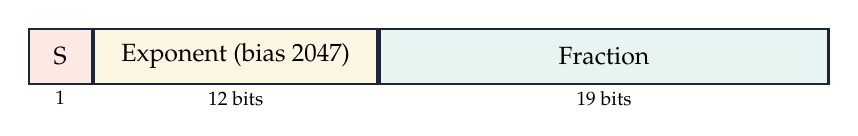
\begin{tikzpicture}[font=\small]
\node[draw=ink,thick,fill=rose,minimum width=8mm,minimum height=7mm] (s) {S};
\node[draw=ink,thick,fill=goldbg,minimum width=36mm,minimum height=7mm,right=0pt of s] (e) {Exponent (bias 2047)};
\node[draw=ink,thick,fill=mist,minimum width=57mm,minimum height=7mm,right=0pt of e] (f) {Fraction};
\node[tk,below=1pt of s]{1}; \node[tk,below=1pt of e]{12 bits}; \node[tk,below=1pt of f]{19 bits};
\end{tikzpicture}}
\begin{enumerate}
\item Precision: 20 significant bits (hidden 1 + 19) $\Rightarrow$ relative precision $2^{-19}\approx1.9\times10^{-6}$, i.e.\ about $19\times\log_{10}2\approx5.7$ (5--6) decimal digits. Representable magnitudes span roughly $10^{-622}$ (denormal) / $10^{-616}$ (normal) to $10^{616}$ (parts ii, iii).
\item Smallest $=1.0\times2^{-2046}\approx1.24\times10^{-616}$; \ Largest $=(2-2^{-19})\times2^{2047}\approx3.23\times10^{616}$.
\item Denormal (exponent field $=0$, hidden bit $0$), slides' formula: $x=(-1)^S\times(0+\text{Fraction})\times2^{-\text{Bias}}$. The smallest non-zero fraction is $0.00\ldots01_2=2^{-19}$, so
smallest denormal $=2^{-19}\times2^{-2047}=2^{-2066}\approx1.18\times10^{-622}$.
\begin{note}Real IEEE-754 hardware scales denormals by $2^{1-\text{Bias}}$ (so they join smoothly with the smallest normal $2^{-2046}$), which would give $2^{-19}\times2^{-2046}=2^{-2065}$. The answer above follows the course slides, which use $2^{-\text{Bias}}$.\end{note}
\end{enumerate}
\end{solution}

%---------------------------------------------------------------- AR08
\begin{question}{2022--2023 \textbullet\ Q8(c)}{CSE 305 \textbullet\ 25/04/2024 \textbullet\ AR08}{10 + 10}
Consider two normalized floating point numbers f1 and f2 that are represented as IEEE single precision floats. This defines two 32-bit strings.
\begin{enumerate}
\item Suppose f1 is less than f2, that is, f1 $<$ f2. If the same two 32-bit strings were treated as unsigned integers (call them i1 and i2, respectively), can we conclude that i1 $<$ i2?
\item Similar to (i), if the two 32-bit strings were treated as signed integers j1 and j2, can we conclude that j1 $<$ j2?
\end{enumerate}
\end{question}
\begin{solution}
\sub{Key fact}
An IEEE float is \key{sign--magnitude}: bit 31 is the sign, and bits 30--0 (biased exponent, then fraction) form the magnitude. Because the exponent is biased (unsigned) and placed before the fraction, for two \emph{non-negative} floats a larger value always has a larger 31-bit pattern. Integers, however, read bit 31 differently: unsigned as weight $+2^{31}$, signed (2's complement) as $-2^{31}$, and 2's complement does \emph{not} reverse the order of the remaining bits like sign--magnitude does.

\sub{Case analysis for f1 $<$ f2}
\fig{\small\renewcommand{\arraystretch}{1.25}
\begin{tabular}{llcc}
\toprule
Case & Example (f1, f2) & i1 $<$ i2 ? & j1 $<$ j2 ?\\
\midrule
$0\le$ f1 $<$ f2 & $1.0=\hex{3F800000}$, $2.0=\hex{40000000}$ & \ok & \ok\\
f1 $<0\le$ f2 & $-1.0=\hex{BF800000}$, $1.0=\hex{3F800000}$ & \no\ ($3212836864 > 1065353216$) & \ok\ ($-1082130432<1065353216$)\\
f1 $<$ f2 $<0$ & $-2.0=\hex{C0000000}$, $-1.0=\hex{BF800000}$ & \no\ ($3221225472>3212836864$) & \no\ ($-1073741824>-1082130432$)\\
\bottomrule
\end{tabular}}

\begin{enumerate}
\item \textbf{Unsigned: No.} It holds only when both numbers are non-negative. If f1 is negative its sign bit makes i1 $\ge 2^{31}$, larger than any non-negative f2's pattern; and if both are negative, the one with the larger magnitude (the smaller value f1) has the larger pattern, so i1 $>$ i2.
\item \textbf{Signed: No (not in general).} It works when both are non-negative (same as unsigned) and when f1 $<0\le$ f2 (j1 is a negative integer, j2 non-negative). But when \emph{both are negative}, both integers are negative and the more negative float (larger magnitude) has the larger bit pattern, hence the \emph{larger} signed integer: j1 $>$ j2. The order is reversed.
\end{enumerate}
\ans{(i) No --- i1 $<$ i2 is guaranteed only if both floats are non-negative. (ii) No --- j1 $<$ j2 holds when both are non-negative or f1 is negative and f2 non-negative, but fails when both are negative (order reverses).}
Remark: integer hardware can still sort floats if each pattern is first mapped as ``if sign $=1$ invert all bits, else flip only the sign bit'', and the results are compared as unsigned integers --- the reason IEEE put the sign first and used a biased exponent.
\end{solution}

%---------------------------------------------------------------- AR09
\begin{question}{2021--2022 \textbullet\ Q5(c)}{CSE 305 \textbullet\ 06/04/2023 \textbullet\ AR09}{10}
Discuss how can subword parallelism be used to accelerate common operations, such as matrix multiplication or image processing?
\end{question}
\begin{solution}
\sub{Idea}
\key{Subword parallelism} (data-level parallelism / SIMD, e.g.\ x86 SSE/AVX) partitions one wide register and one wide adder/multiplier into independent lanes. A single instruction then operates on all lanes at once: a 128-bit adder can do sixteen 8-bit, eight 16-bit, four 32-bit or two 64-bit additions (carries are simply cut at lane boundaries).
\fig{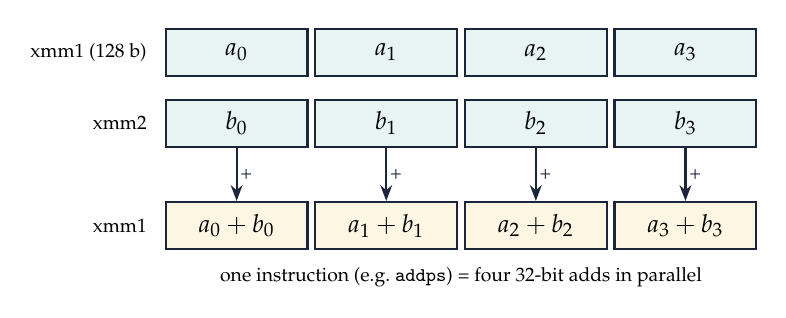
\begin{tikzpicture}[font=\small]
\foreach \i in {0,1,2,3}{
 \node[draw=ink,thick,fill=mist,minimum width=18mm,minimum height=6mm] (a\i) at (\i*1.9,0) {$a_\i$};
 \node[draw=ink,thick,fill=mist,minimum width=18mm,minimum height=6mm] (b\i) at (\i*1.9,-0.9) {$b_\i$};
 \node[draw=ink,thick,fill=goldbg,minimum width=18mm,minimum height=6mm] (c\i) at (\i*1.9,-2.2) {$a_\i+b_\i$};
 \draw[wire] (b\i.south)--node[tk,right]{+}(c\i.north);}
\node[tk,anchor=east] at (-1.1,0) {xmm1 (128 b)};
\node[tk,anchor=east] at (-1.1,-0.9) {xmm2};
\node[tk,anchor=east] at (-1.1,-2.2) {xmm1};
\node[tk] at (2.85,-2.85) {one instruction (e.g.\ \texttt{addps}) = four 32-bit adds in parallel};
\end{tikzpicture}}
\sub{Matrix multiplication (slides: DGEMM with AVX)}
\begin{itemize}
\item In $C = C + A\times B$ the same multiply-add is done on many independent elements. With 256-bit AVX registers, four doubles of a column of $C$ are kept in one register: \texttt{\_mm256\_load\_pd} loads 4 elements of $A$, \texttt{\_mm256\_broadcast\_sd} makes 4 copies of $B[k][j]$, then \texttt{\_mm256\_mul\_pd} and \texttt{\_mm256\_add\_pd} (\texttt{vmulpd}, \texttt{vaddpd}) update 4 results per instruction.
\item The loop over $i$ advances by 4, so the number of FP instructions (and loop overhead) drops about $4\times$; P\&H reports $\approx3.8\times$ speed-up for DGEMM from this change alone.
\end{itemize}
\sub{Image / media processing}
\begin{itemize}
\item Pixels are 8-bit (or 16-bit) values, so a 128-bit register holds 16 pixels. Brightness change, blending/alpha compositing, filtering and colour conversion apply the same operation to every pixel: one SIMD instruction processes 16 pixels, giving up to $16\times$ fewer instructions.
\item Media SIMD adds \key{saturating} arithmetic (e.g.\ $250+10\to255$, not wrap-around to 4), packed min/max/average, and pack/unpack/shuffle to rearrange subwords --- all common in graphics and audio.
\end{itemize}
Benefits: no extra datapath width is needed (the existing wide adder is reused), fewer instructions fetched/decoded, better use of memory bandwidth because whole cache blocks of data are consumed per instruction. Requirement: data must be laid out contiguously and aligned, and the work must be the same for all lanes.
\end{solution}

%---------------------------------------------------------------- AR10
\begin{question}{2021--2022 \textbullet\ Q6(c)}{CSE 305 \textbullet\ 06/04/2023 \textbullet\ AR10}{10}
Draw the block diagram of 32-bit combined multiplication and division hardware which uses 32-bit ALU, and briefly mention functions of different components of this hardware.
\end{question}
\begin{solution}
The refined (optimized) multiplier and the optimized divider have the same structure: a 32-bit register, a 32-bit ALU and a 64-bit shift register. The slides note that the same hardware can be used for both. Only the ALU operation (add or subtract) and the shift direction differ.
\fig{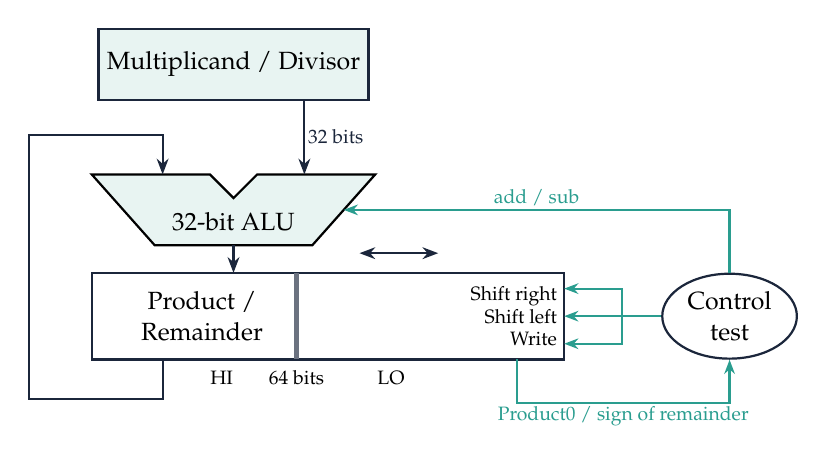
\begin{tikzpicture}[font=\small]
\node[blkm,minimum width=34mm,minimum height=9mm] (mc) at (0,3) {Multiplicand / Divisor};
\draw[thick,fill=mist] (-1.8,1.6) -- (-0.3,1.6) -- (0,1.3) -- (0.3,1.6) -- (1.8,1.6) -- (1.0,0.7) -- (-1.0,0.7) -- cycle;
\node at (0,1.0) {32-bit ALU};
\draw[wire] (0.9,2.55) -- node[right,tk]{32 bits} (0.9,1.6);
\node[blk,minimum width=60mm,minimum height=11mm] (pr) at (1.2,-0.2) {};
\node[align=center] at (-0.4,-0.2) {Product /\\Remainder};
\node[tk] at (-0.15,-0.98) {HI};
\node[tk] at (2.0,-0.98) {LO};
\node[tk] at (0.8,-0.98) {64 bits};
\draw[slate,line width=2pt] (0.8,-0.75) -- (0.8,0.35);
\node[tk,anchor=east,align=right] at (4.15,-0.2) {Shift right\\Shift left\\Write};
\draw[wire,<->] (1.6,0.6) -- (2.6,0.6);
\draw[wire] (0,0.7) -- (0,0.35);
\draw[wire] (-0.9,-0.75) -- (-0.9,-1.25) -- (-2.6,-1.25) -- (-2.6,2.1) -- (-0.9,2.1) -- (-0.9,1.6);
\node[oval] (ct) at (6.3,-0.2) {Control\\test};
\draw[ctl] (ct.west) -- ++(-0.5,0) |- (4.2,0.15);
\draw[ctl] (ct.west) -- ++(-0.5,0) |- (4.2,-0.2);
\draw[ctl] (ct.west) -- ++(-0.5,0) |- (4.2,-0.55);
\draw[ctl] (ct.north) |- node[above,tk,pos=0.75]{add / sub} (1.4,1.15);
\draw[ctl] (3.6,-0.75) -- (3.6,-1.3) -| node[below,tk,pos=0.25]{Product0 / sign of remainder} (ct.south);
\end{tikzpicture}}
\begin{itemize}
\item \key{Multiplicand/Divisor register (32 bits)}: holds the multiplicand or the divisor. It never shifts.
\item \key{32-bit ALU}: when multiplying, it adds the multiplicand to the left half (HI). When dividing, it subtracts the divisor from HI, and adds it back to restore if the result is negative.
\item \key{64-bit Product/Remainder register}:
  \begin{itemize}
  \item Multiply: starts as HI $=0$, LO $=$ multiplier. It \emph{shifts right} each step and ends holding the 64-bit product.
  \item Divide: starts with the dividend in LO and \emph{shifts left}; each new quotient bit enters at the right end. At the end HI $=$ remainder and LO $=$ quotient, which are the MIPS HI/LO registers. A final right shift of the left half corrects the remainder.
  \end{itemize}
\item \key{Control test}: looks at Product0 (multiply) or the sign of the new remainder (divide). From that it chooses add or subtract, write, and the shift direction. It also counts the 32 repetitions.
\end{itemize}
\end{solution}

%---------------------------------------------------------------- AR11
\begin{question}{2021--2022 \textbullet\ Q8(b)}{CSE 305 \textbullet\ 06/04/2023 \textbullet\ AR11}{14}
Consider representing the set of consecutive positive integers $\{1, 2, 3, 4, \ldots, n\}$ using IEEE single precision floating point (8-bit exponent and 23-bit mantissa). Find the largest $n$ such that every number in the above set can be represented.
\end{question}
\begin{solution}
A normalized single has a \key{24-bit significand} ($1$ hidden bit $+$ 23 fraction bits): $x = 1.f_1f_2\ldots f_{23}\times2^{e}$.
\begin{itemize}
\item An integer $k$ with $2^{m}\le k<2^{m+1}$ is $1.b_{m-1}\ldots b_0\times2^{m}$: it needs $m$ fraction bits. So every integer with at most 24 significant bits ($k<2^{24}$, i.e.\ $m\le23$) is exact. The exponent range ($e\le127$) is no limit here.
\item $2^{24} = 1.0\times2^{24}$ is also exact (fraction all 0, $E=24+127=151$).
\item $2^{24}+1 = 1.\underbrace{00\ldots0}_{23}1_2\times2^{24}$ needs \textbf{24} fraction bits; only 23 exist, so it cannot be represented (it rounds to $2^{24}$; above $2^{24}$ the spacing of floats is 2).
\end{itemize}
\begin{center}\small\begin{tabular}{lll}
\toprule
Integer & Single-precision pattern & exact?\\
\midrule
$2^{24}-1 = 16\,777\,215$ & \texttt{0 10010110 11111111111111111111111} $=\hex{4B7FFFFF}$ & \ok\\
$2^{24} = 16\,777\,216$ & \texttt{0 10010111 00000000000000000000000} $=\hex{4B800000}$ & \ok\\
$2^{24}+1 = 16\,777\,217$ & would need fraction \texttt{0\ldots0}\,\texttt{1} (24 bits) & \no\ (rounds to $2^{24}$)\\
$2^{24}+2 = 16\,777\,218$ & \texttt{0 10010111 00000000000000000000001} $=\hex{4B800001}$ & \ok\\
\bottomrule
\end{tabular}\end{center}
\ans{$n = 2^{24} = 16\,777\,216$. All of $1,\ldots,2^{24}$ are exactly representable; $2^{24}+1$ is the first integer that is not.}
\end{solution}

%---------------------------------------------------------------- AR12
\begin{question}{2020--2021 \textbullet\ Q10(c)}{CSE 305 \textbullet\ 24/09/2022 \textbullet\ AR12}{5}
Briefly describe how to perform a signed multiplication operation.
\end{question}
\begin{solution}
\sub{Sign--magnitude method (P\&H)}
\begin{enumerate}[label=\textbf{\arabic*.}]
\item Record the signs and convert both operands to positive (2's-complement negate a negative operand).
\item Multiply the magnitudes with the unsigned shift-and-add multiplier, using $n-1$ iterations for the magnitude bits (31 for MIPS) --- the sign bits are left out.
\item Product sign $=$ sign(multiplicand) $\oplus$ sign(multiplier); if it is 1, negate the $2n$-bit product.
\end{enumerate}
Example (4-bit): $(-3)\times5$: $|{-3}|=0011$, $0011\times0101 = 0000\,1111$ (15); signs differ $\Rightarrow$ negate: $1111\,0001 = -15$.

\sub{Alternatives}
Keep the operands in 2's complement and \emph{sign-extend} the partial products (shifting the product right arithmetically), subtracting at the last step for a negative multiplier; \key{Booth's algorithm} does this efficiently by examining bit pairs $(q_0,q_{-1})$: $10\Rightarrow$ subtract multiplicand, $01\Rightarrow$ add, $00/11\Rightarrow$ nothing, then arithmetic shift right. In MIPS, \ins{mult} gives the signed 64-bit product in HI/LO (\ins{multu} for unsigned).
\end{solution}

%---------------------------------------------------------------- AR13
\begin{question}{2020--2021 \textbullet\ Q12(c)}{CSE 305 \textbullet\ 24/09/2022 \textbullet\ AR13}{9}
Briefly explain the importance of guard digit, round digit, and sticky bit during rounding an intermediate floating point number.
\end{question}
\begin{solution}
During alignment and normalization, bits are shifted out to the right of the significand. If they were simply dropped the result could be off by more than half an ulp. IEEE 754 therefore keeps extra bits in the intermediate result (slides: ``extra bits of precision (guard, round, sticky)''):
\begin{itemize}
\item \key{Guard bit}: the first bit beyond the kept significand. It is needed because after a subtraction or a carry the result may be shifted \emph{left} one place during normalization; the guard bit then becomes the new LSB instead of a lost 0.
\item \key{Round bit}: the second extra bit. After a possible normalization shift it still leaves one bit to decide the rounding direction (above/below half).
\item \key{Sticky bit}: the OR of \emph{all} bits shifted past the round bit. It records whether anything non-zero was lost, which distinguishes an exact half-way case from ``slightly more than half''. This makes round-to-nearest-even exact.
\end{itemize}
\sub{Effect --- decimal example (3 significant digits)}
$2.56\times10^{0}+2.34\times10^{2}$: aligned, $0.0256\times10^2$. \emph{With} guard (5) and round (6): $2.3400+0.0256=2.3656\to\mathbf{2.37}\times10^2$ (correct). \emph{Without} them: $2.34+0.02=2.36\times10^2$ --- off by 1 in the last digit.

\sub{Round-to-nearest-even decision (G R S after the LSB)}
{\small\begin{tabular}{@{}ll@{}}
\texttt{0xx} & below half $\Rightarrow$ truncate\\
\texttt{100} & exactly half $\Rightarrow$ round to make the LSB even\\
\texttt{101}, \texttt{11x} & above half $\Rightarrow$ round up (add 1 ulp)
\end{tabular}}

Binary example: $1.0100\,|\,\texttt{G=1 R=0 S=1}$ is above half, so it rounds up to $1.0101$. Without the sticky bit it would look like an exact tie ($\texttt{10}$) and round-to-even would give $1.0100$ --- wrong.
\ans{Guard and round bits keep two extra bits so that normalization and rounding do not lose accuracy; the sticky bit remembers whether any non-zero bit was lost beyond them, so ties are detected correctly. Together they let the hardware round as if the result had been computed exactly.}
\end{solution}

%---------------------------------------------------------------- AR14
\begin{question}{2020--2021 \textbullet\ Q13(a)}{CSE 305 \textbullet\ 24/09/2022 \textbullet\ AR14}{4$\times$4}
Consider a 32-bit system where 24 bits are reserved for fraction, one bit for sign, and the rest for exponent. Answer the following questions.
\begin{enumerate}
\item Why is bias used during the floating point representation?
\item What should be the value of the bias for this system? Why?
\item What are the smallest and the largest absolute values that can be stored in this system?
\item What is the smallest denormalized number that can be stored using this system?
\end{enumerate}
\end{question}
\begin{solution}
\sub{Format}
$32-1-24 = 7$ exponent bits.
\fig{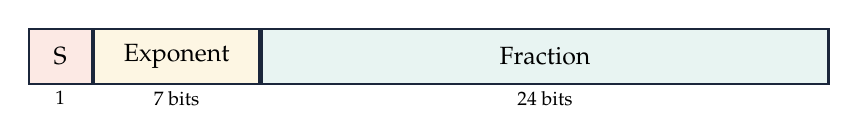
\begin{tikzpicture}[font=\small]
\node[draw=ink,thick,fill=rose,minimum width=8mm,minimum height=7mm] (s) {S};
\node[draw=ink,thick,fill=goldbg,minimum width=21mm,minimum height=7mm,right=0pt of s] (e) {Exponent};
\node[draw=ink,thick,fill=mist,minimum width=72mm,minimum height=7mm,right=0pt of e] (f) {Fraction};
\node[tk,below=1pt of s]{1}; \node[tk,below=1pt of e]{7 bits}; \node[tk,below=1pt of f]{24 bits};
\end{tikzpicture}}
\begin{enumerate}
\item \textbf{Why bias:}
\begin{itemize}
\item The exponent must hold negative and positive values. Storing it as \emph{(true exponent $+$ bias)} makes the field an \key{unsigned} number, so floats can be compared/sorted with simple integer hardware (sign, then exponent, then fraction) --- no 2's-complement exponent handling.
\item The smallest exponent field becomes all 0s (used for $0$ and denormals) and the largest all 1s ($\infty$, NaN).
\end{itemize}
\item \textbf{Bias $=2^{7-1}-1=63$.} With fields 0 and 127 reserved, $E=1\ldots126$ gives true exponents $-62\ldots+63$: the middle of the field, splitting the range almost symmetrically so that $2^{e_{\max}}\approx1/2^{e_{\min}}$ (the reciprocal of the smallest normal number does not overflow), following the IEEE rule bias $=2^{k-1}-1$.
\item Smallest normal $=1.0\times2^{-62}\approx2.17\times10^{-19}$; \ Largest $=(2-2^{-24})\times2^{63}\approx1.84\times10^{19}$.
\item Denormal (exponent field $=0$), slides' formula $x=(-1)^S\times(0+\text{Fraction})\times2^{-\text{Bias}}$: smallest denormal $=0.00\ldots01_2\times2^{-63}=2^{-24}\times2^{-63}=2^{-87}\approx6.46\times10^{-27}$.
\begin{note}Real IEEE-754 hardware uses $2^{1-\text{Bias}}$ for denormals, which would give $2^{-24}\times2^{-62}=2^{-86}$. The answer follows the course slides ($2^{-\text{Bias}}$).\end{note}
\end{enumerate}
\end{solution}

%---------------------------------------------------------------- AR15
\begin{question}{2019--2020 \textbullet\ Q4(a)}{CSE 305 \textbullet\ 18/09/2021 \textbullet\ AR15}{6 + 5 + 4}
Suppose, you are working in a system where 16 bits are used to represent a floating-point value. The largest absolute floating-point value that can be represented by the system is $1.11\ldots1_{two}\times2^{63}$ while the smallest absolute floating point value that can be represented by the system is $1.00\ldots0_{two}\times2^{-62}$.
\begin{enumerate}
\item Show the floating-point representation format (bit distribution among sign, exponent and fraction portion) of this system.
\item Show the floating-point representation for the number $-110.11_{two}\times2^{1}$ in this system assuming an appropriate bias.
\item What is the smallest absolute denormalized floating-point value that can be stored in this system?
\end{enumerate}
\end{question}
\begin{solution}
\sub{Rules (IEEE-754 style, $k$ exponent bits)}
Bias $=2^{k-1}-1$; fields all-0 (zero/denormals) and all-1 ($\infty$/NaN) reserved, so normal exponents run from $1-\text{bias}$ to $+\text{bias}$. Denormal (slides): $x=(-1)^S\times(0+\text{Fraction})\times2^{-\text{Bias}}$.
\begin{enumerate}
\item True exponents run from $-62$ to $+63$: $126$ values, plus the two reserved codes $=128=2^7$ $\Rightarrow$ \textbf{7} exponent bits with bias $63$ ($E=1\ldots126$). Remaining: $16-1-7=$ \textbf{8} fraction bits.
\fig{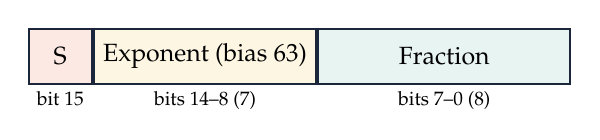
\begin{tikzpicture}[font=\small]
\node[draw=ink,thick,fill=rose,minimum width=8mm,minimum height=7mm] (s) {S};
\node[draw=ink,thick,fill=goldbg,minimum width=28mm,minimum height=7mm,right=0pt of s] (e) {Exponent (bias 63)};
\node[draw=ink,thick,fill=mist,minimum width=32mm,minimum height=7mm,right=0pt of e] (f) {Fraction};
\node[tk,below=1pt of s]{bit 15}; \node[tk,below=1pt of e]{bits 14--8 (7)}; \node[tk,below=1pt of f]{bits 7--0 (8)};
\end{tikzpicture}}
\item $-110.11_2\times2^1 = -1.1011_2\times2^{3}$ \ ($=-13.5$). \ $S=1$, $E=3+63=66=\texttt{1000010}$, $F=\texttt{10110000}$.
\fig{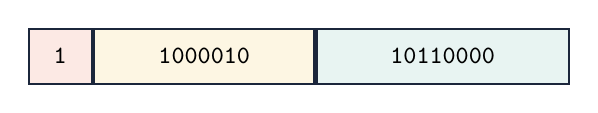
\begin{tikzpicture}[font=\small\ttfamily]
\node[draw=ink,thick,fill=rose,minimum width=8mm,minimum height=7mm] (s) {1};
\node[draw=ink,thick,fill=goldbg,minimum width=28mm,minimum height=7mm,right=0pt of s] (e) {1000010};
\node[draw=ink,thick,fill=mist,minimum width=32mm,minimum height=7mm,right=0pt of e] (f) {10110000};
\end{tikzpicture}}
\ans{$-110.11_2\times2^1 \to \texttt{1 1000010 10110000} = \hex{C2B0}$}
\item Smallest denormal $=0.00000001_2\times2^{-63}=2^{-8}\times2^{-63}=2^{-71}\approx4.24\times10^{-22}$.
\begin{note}Real IEEE-754 hardware uses $2^{1-\text{Bias}}$ for denormals, which would give $2^{-8}\times2^{-62}=2^{-70}$. The answer follows the course slides ($2^{-\text{Bias}}$).\end{note}
\end{enumerate}
\end{solution}

%---------------------------------------------------------------- AR16
\begin{question}{2019--2020 \textbullet\ Q4(c)}{CSE 305 \textbullet\ 18/09/2021 \textbullet\ AR16}{8}
Consider the following C code fragment.
\begin{ccode}
if(a>b)
   c = c-(c*e)/d;
else
   c = c+d;
\end{ccode}
If $a, b, c, d$ and $e$ are variables of type \emph{double} and their values are already loaded in registers \reg{f2}, \reg{f4}, \$6, \reg{f8} and \reg{f10} respectively, then write down the equivalent MIPS assembly code for it. Use the least number of MIPS instructions possible.
\end{question}
\begin{solution}
\sub{Rules used (slides: FP instructions in MIPS)}
All variables are double, so every operation uses the \ins{.d} forms (\ins{mul.d}, \ins{div.d}, \ins{sub.d}, \ins{add.d}); the comparison \ins{c.lt.d} sets the FP condition flag, tested by \ins{bc1t}/\ins{bc1f}. There is no ``greater than'' compare, so $a>b$ is tested as $b<a$.
\begin{mips}
      c.lt.d $f4, $f2            # flag = (b < a)  i.e. (a > b)
      bc1f   Else                # not (a > b) -> else part
      mul.d  $f12, $f6, $f10     # $f12 = c * e
      div.d  $f12, $f12, $f8     # $f12 = (c*e) / d
      sub.d  $f6, $f6, $f12      # c = c - (c*e)/d
      j      Exit
Else: add.d  $f6, $f6, $f8       # c = c + d
Exit:
\end{mips}
7 instructions (minimum: one compare, one conditional branch, one jump to skip the else, plus four arithmetic ops). \reg{f12} (pair \reg{f12}/\reg{f13}) is a temporary.
\begin{note}The scan prints the register of $c$ as ``\$6''; since $c$ is a double it must be the FP register \reg{f6} (an integer register cannot hold a double) --- treated as a misprint.\end{note}
\end{solution}

%---------------------------------------------------------------- AR17
\begin{question}{2018--2019 \textbullet\ Q5(b)}{CSE 305 \textbullet\ 29/10/2019 \textbullet\ AR17}{8}
Consider a 16-bit floating point representation system, where the exponent is 4 bits long. With this system, represent the floating point numbers $(-1.25)_{10}$ and $(0.375)_{10}$ into a bit string of length 16 using appropriate bias.
\end{question}
\begin{solution}
\sub{Format (IEEE-754 style)}
16 bits $=$ 1 sign $+$ 4 exponent $+$ 11 fraction. \ Bias $=2^{4-1}-1 = 7$ ($E=1\ldots14$ for normal numbers, true exponent $-6\ldots+7$; $0000$ and $1111$ reserved). Value $=(-1)^S\times1.F\times2^{E-7}$.
\fig{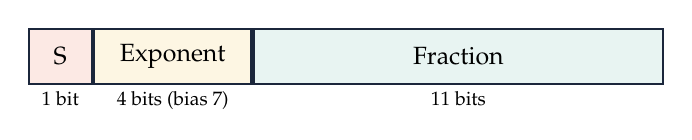
\begin{tikzpicture}[font=\small]
\node[draw=ink,thick,fill=rose,minimum width=8mm,minimum height=7mm] (s) {S};
\node[draw=ink,thick,fill=goldbg,minimum width=20mm,minimum height=7mm,right=0pt of s] (e) {Exponent};
\node[draw=ink,thick,fill=mist,minimum width=52mm,minimum height=7mm,right=0pt of e] (f) {Fraction};
\node[tk,below=1pt of s]{1 bit}; \node[tk,below=1pt of e]{4 bits (bias 7)}; \node[tk,below=1pt of f]{11 bits};
\end{tikzpicture}}
\sub{Encoding}
\begin{itemize}
\item $-1.25 = -1.01_2\times2^{0}$: $S=1$, $E=0+7=7=\texttt{0111}$, $F=\texttt{01000000000}$.
\item $0.375 = 0.011_2 = 1.1_2\times2^{-2}$: $S=0$, $E=-2+7=5=\texttt{0101}$, $F=\texttt{10000000000}$.
\end{itemize}
\fig{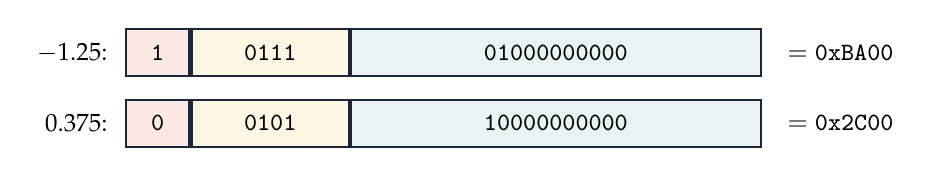
\begin{tikzpicture}[font=\small\ttfamily]
\node[font=\small,anchor=east] at (-0.1,0) {$-1.25$:};
\node[draw=ink,thick,fill=rose,minimum width=8mm,minimum height=6mm,anchor=west] (s) at (0,0) {1};
\node[draw=ink,thick,fill=goldbg,minimum width=20mm,minimum height=6mm,right=0pt of s] (e) {0111};
\node[draw=ink,thick,fill=mist,minimum width=52mm,minimum height=6mm,right=0pt of e] (f) {01000000000};
\node[font=\small,right=2mm of f] {$=\hex{BA00}$};
\node[font=\small,anchor=east] at (-0.1,-0.9) {$0.375$:};
\node[draw=ink,thick,fill=rose,minimum width=8mm,minimum height=6mm,anchor=west] (s2) at (0,-0.9) {0};
\node[draw=ink,thick,fill=goldbg,minimum width=20mm,minimum height=6mm,right=0pt of s2] (e2) {0101};
\node[draw=ink,thick,fill=mist,minimum width=52mm,minimum height=6mm,right=0pt of e2] (f2) {10000000000};
\node[font=\small,right=2mm of f2] {$=\hex{2C00}$};
\end{tikzpicture}}
\ans{$-1.25 \to \texttt{1 0111 01000000000}$ $(\hex{BA00})$; \quad $0.375\to\texttt{0 0101 10000000000}$ $(\hex{2C00})$.}
\end{solution}

%---------------------------------------------------------------- AR18
\begin{question}{2018--2019 \textbullet\ Q5(c)}{CSE 305 \textbullet\ 29/10/2019 \textbullet\ AR18}{5}
Determine the decimal value of the floating point number represented by the hexadecimal value $(\texttt{DF80 7500})_{16}$ according to IEEE 754 single precision floating point format.
\end{question}
\begin{solution}
Split the 32 bits into $S$ (1) $|$ $E$ (8) $|$ $F$ (23); for $1\le E\le254$: value $=(-1)^S(1+F/2^{23})\,2^{E-127}$.
\fig{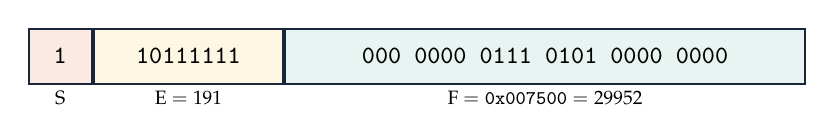
\begin{tikzpicture}[font=\small\ttfamily]
\node[draw=ink,thick,fill=rose,minimum width=8mm,minimum height=7mm] (s) {1};
\node[draw=ink,thick,fill=goldbg,minimum width=24mm,minimum height=7mm,right=0pt of s] (e) {10111111};
\node[draw=ink,thick,fill=mist,minimum width=66mm,minimum height=7mm,right=0pt of e] (f) {000 0000 0111 0101 0000 0000};
\node[tk,below=1pt of s]{S}; \node[tk,below=1pt of e]{E $=191$}; \node[tk,below=1pt of f]{F $=\hex{007500}=29952$};
\end{tikzpicture}}
$\texttt{DF807500} = \texttt{1101\,1111\,1000\,0000\,0111\,0101\,0000\,0000}$.
$S=1$ (negative); $E=\texttt{10111111}=191\Rightarrow$ exponent $191-127=64$;
$1.F = 1.00000000111010100000000_2 = 1+2^{-9}+2^{-10}+2^{-11}+2^{-13}+2^{-15} = 1.003570556640625$.
\[ x = -1.003570556640625\times2^{64} = -18\,512\,609\,218\,259\,845\,120 \]
\ans{$(\texttt{DF807500})_{16} = -1.003570556640625\times2^{64}\approx -1.8513\times10^{19}$.}
\end{solution}

%---------------------------------------------------------------- AR19
\begin{question}{2018--2019 \textbullet\ Q6(b)}{CSE 305 \textbullet\ 29/10/2019 \textbullet\ AR19}{15}
Suppose you have a 4-bit ALU and you are required to perform a division operation, where the dividend is \texttt{11001001} and the divisor is \texttt{1011}. Show the division process step by step along with the value of each relevant register at each step.
\end{question}
\begin{solution}
\sub{Hardware and algorithm: the Optimized Divider (slides)}
With a 4-bit ALU, $n=4$: a 4-bit \textbf{Divisor} register and an 8-bit \textbf{Remainder} register (left half Rem$_{hi}$, right half Rem$_{lo}$). There is no Quotient register; quotient bits enter at the right end of the Remainder.
\textbf{0.}~Remainder $\leftarrow$ dividend, shift Remainder left 1. Repeat $n$ times: \textbf{1.}~Rem$_{hi}\leftarrow$ Rem$_{hi}-$Divisor; \textbf{2a.}~if $\ge0$: shift Remainder left, new rightmost bit $=1$; \textbf{2b.}~if $<0$: restore (Rem$_{hi}+$Divisor), shift Remainder left, new rightmost bit $=0$. \textbf{3.}~Shift Rem$_{hi}$ right 1. Result: Rem$_{lo}=$ quotient, Rem$_{hi}=$ remainder.

\textbf{Why shift first?} The first quotient bit has weight $2^{n-1}$: it asks whether Divisor$\times2^{n-1}$ fits, i.e.\ it compares the Divisor with the dividend's top $n{+}1$ bits, which is what the left half holds after one left shift. Subtracting from the unshifted left half would test Divisor$\times2^{n}$, a quotient bit an $n$-bit quotient cannot have; if that test succeeds the division overflows (as happens here). The extra left shift is undone by the final right shift of Rem$_{hi}$.
\fig{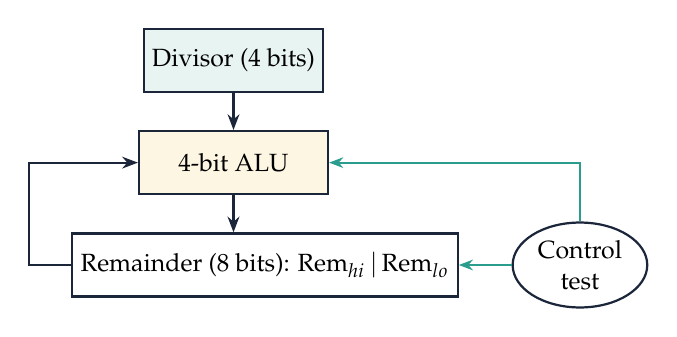
\begin{tikzpicture}[font=\small]
 \node[blkm,minimum width=20mm] (dv) at (0,0) {Divisor (4 bits)};
 \node[blkg,minimum width=24mm] (al) at (0,-1.3) {4-bit ALU};
 \node[blk,minimum width=46mm] (rm) at (0.4,-2.6) {Remainder (8 bits): Rem$_{hi}$\,$|$\,Rem$_{lo}$};
 \node[oval] (ct) at (4.4,-2.6) {Control\\test};
 \draw[wire] (dv) -- (al);
 \draw[wire] (al) -- ($(rm.north)+(-0.4,0)$);
 \draw[wire] ($(rm.west)$) -| (-2.6,-1.3) -- (al.west);
 \draw[ctl] (ct.west) -- (rm.east);
 \draw[ctl] (ct.north) |- (al.east);
\end{tikzpicture}}

\sub{Divide-overflow check}
The quotient can have only $n=4$ bits (it lives in Rem$_{lo}$). That works only if the dividend's left half is smaller than the divisor. Here Rem$_{hi}=\texttt{1100}=12 \ge \texttt{1011}=11$, so the true quotient $201\div11=18=\texttt{10010}_2$ needs 5 bits: this is a \key{divide overflow}. Real hardware checks Rem$_{hi}\ge$ Divisor before starting and signals overflow. Below the 4-bit trace is shown as asked, and then the same algorithm on a 5-bit ALU, which gives the correct result.

\sub{(i) Strict 4-bit trace: $\texttt{11001001}_2 \div \texttt{1011}_2$}
The first left shift pushes the dividend's leading 1 out of the 8-bit register, so the hardware is already working on the wrong number. Changed values are in \textcolor{coral}{\textbf{coral}}; a negative difference is signalled by the ALU's borrow.
\fig{\footnotesize\setlength{\tabcolsep}{4pt}\begin{tabular}{c>{\raggedright\arraybackslash}p{50mm}ccc}
\toprule
Iter. & Step & Divisor & Remainder (Rem$_{hi}$\,$|$\,Rem$_{lo}$) & sign\\
\midrule
0 & Initial values & \texttt{1011} & \texttt{1100}\,$|$\,\texttt{1001} & \\
 & Shift Rem left 1 (MSB 1 lost) & \texttt{1011} & \textcolor{coral}{\textbf{\texttt{1001}}}\,$|$\,\textcolor{coral}{\textbf{\texttt{0010}}} & \\
\midrule
1 & 1: Rem$_{hi}$ $\leftarrow$ Rem$_{hi}-$Div & \texttt{1011} & \textcolor{coral}{\textbf{\texttt{1110}}}\,$|$\,\texttt{0010} & $<0$\\
 & 2b: Rem$<$0: $+$Div, sll Rem, Rem$_0{=}0$ & \texttt{1011} & \textcolor{coral}{\textbf{\texttt{0010}}}\,$|$\,\textcolor{coral}{\textbf{\texttt{0100}}} & \\
\midrule
2 & 1: Rem$_{hi}$ $\leftarrow$ Rem$_{hi}-$Div & \texttt{1011} & \textcolor{coral}{\textbf{\texttt{0111}}}\,$|$\,\texttt{0100} & $<0$\\
 & 2b: Rem$<$0: $+$Div, sll Rem, Rem$_0{=}0$ & \texttt{1011} & \textcolor{coral}{\textbf{\texttt{0100}}}\,$|$\,\textcolor{coral}{\textbf{\texttt{1000}}} & \\
\bottomrule
\end{tabular}}
\fig{\footnotesize\setlength{\tabcolsep}{4pt}\begin{tabular}{c>{\raggedright\arraybackslash}p{50mm}ccc}
\toprule
Iter. & Step & Divisor & Remainder (Rem$_{hi}$\,$|$\,Rem$_{lo}$) & sign \ \textit{(cont.)}\\
\midrule
3 & 1: Rem$_{hi}$ $\leftarrow$ Rem$_{hi}-$Div & \texttt{1011} & \textcolor{coral}{\textbf{\texttt{1001}}}\,$|$\,\texttt{1000} & $<0$\\
 & 2b: Rem$<$0: $+$Div, sll Rem, Rem$_0{=}0$ & \texttt{1011} & \textcolor{coral}{\textbf{\texttt{1001}}}\,$|$\,\textcolor{coral}{\textbf{\texttt{0000}}} & \\
\midrule
4 & 1: Rem$_{hi}$ $\leftarrow$ Rem$_{hi}-$Div & \texttt{1011} & \textcolor{coral}{\textbf{\texttt{1110}}}\,$|$\,\texttt{0000} & $<0$\\
 & 2b: Rem$<$0: $+$Div, sll Rem, Rem$_0{=}0$ & \texttt{1011} & \textcolor{coral}{\textbf{\texttt{0010}}}\,$|$\,\textcolor{coral}{\textbf{\texttt{0000}}} & \\
\midrule
 & 3: Shift Rem$_{hi}$ right 1 & \texttt{1011} & \textcolor{coral}{\textbf{\texttt{0001}}}\,$|$\,\texttt{0000} & \\
\bottomrule
\end{tabular}}
The 4-bit hardware ends with quotient $\texttt{0000}$ and remainder $\texttt{0001}$, which is \textbf{wrong} ($11\times0+1\ne201$). This is the divide overflow: an $n$-bit divider cannot produce an $(n{+}1)$-bit quotient.

\sub{(ii) Same algorithm on a 5-bit ALU (correct result)}
With $n=5$ the dividend is $\texttt{00\,1100\,1001}$ (10-bit Remainder) and the Divisor is $\texttt{01011}$; now Rem$_{hi}=\texttt{00110}<\texttt{01011}$, so no overflow.
\fig{\footnotesize\setlength{\tabcolsep}{4pt}\begin{tabular}{c>{\raggedright\arraybackslash}p{50mm}ccc}
\toprule
Iter. & Step & Divisor & Remainder (Rem$_{hi}$\,$|$\,Rem$_{lo}$) & sign\\
\midrule
0 & Initial values & \texttt{01011} & \texttt{00110}\,$|$\,\texttt{01001} & \\
 & Shift Rem left 1 & \texttt{01011} & \textcolor{coral}{\textbf{\texttt{01100}}}\,$|$\,\textcolor{coral}{\textbf{\texttt{10010}}} & \\
\midrule
1 & 1: Rem$_{hi}$ $\leftarrow$ Rem$_{hi}-$Div & \texttt{01011} & \textcolor{coral}{\textbf{\texttt{00001}}}\,$|$\,\texttt{10010} & $\ge 0$\\
 & 2a: Rem$\ge$0: sll Rem, Rem$_0{=}1$ & \texttt{01011} & \textcolor{coral}{\textbf{\texttt{00011}}}\,$|$\,\textcolor{coral}{\textbf{\texttt{00101}}} & \\
\midrule
2 & 1: Rem$_{hi}$ $\leftarrow$ Rem$_{hi}-$Div & \texttt{01011} & \textcolor{coral}{\textbf{\texttt{11000}}}\,$|$\,\texttt{00101} & $<0$\\
 & 2b: Rem$<$0: $+$Div, sll Rem, Rem$_0{=}0$ & \texttt{01011} & \textcolor{coral}{\textbf{\texttt{00110}}}\,$|$\,\textcolor{coral}{\textbf{\texttt{01010}}} & \\
\midrule
3 & 1: Rem$_{hi}$ $\leftarrow$ Rem$_{hi}-$Div & \texttt{01011} & \textcolor{coral}{\textbf{\texttt{11011}}}\,$|$\,\texttt{01010} & $<0$\\
 & 2b: Rem$<$0: $+$Div, sll Rem, Rem$_0{=}0$ & \texttt{01011} & \textcolor{coral}{\textbf{\texttt{01100}}}\,$|$\,\textcolor{coral}{\textbf{\texttt{10100}}} & \\
\bottomrule
\end{tabular}}
\fig{\footnotesize\setlength{\tabcolsep}{4pt}\begin{tabular}{c>{\raggedright\arraybackslash}p{50mm}ccc}
\toprule
Iter. & Step & Divisor & Remainder (Rem$_{hi}$\,$|$\,Rem$_{lo}$) & sign \ \textit{(cont.)}\\
\midrule
4 & 1: Rem$_{hi}$ $\leftarrow$ Rem$_{hi}-$Div & \texttt{01011} & \textcolor{coral}{\textbf{\texttt{00001}}}\,$|$\,\texttt{10100} & $\ge 0$\\
 & 2a: Rem$\ge$0: sll Rem, Rem$_0{=}1$ & \texttt{01011} & \textcolor{coral}{\textbf{\texttt{00011}}}\,$|$\,\textcolor{coral}{\textbf{\texttt{01001}}} & \\
\midrule
5 & 1: Rem$_{hi}$ $\leftarrow$ Rem$_{hi}-$Div & \texttt{01011} & \textcolor{coral}{\textbf{\texttt{11000}}}\,$|$\,\texttt{01001} & $<0$\\
 & 2b: Rem$<$0: $+$Div, sll Rem, Rem$_0{=}0$ & \texttt{01011} & \textcolor{coral}{\textbf{\texttt{00110}}}\,$|$\,\textcolor{coral}{\textbf{\texttt{10010}}} & \\
\midrule
 & 3: Shift Rem$_{hi}$ right 1 & \texttt{01011} & \textcolor{coral}{\textbf{\texttt{00011}}}\,$|$\,\texttt{10010} & \\
\bottomrule
\end{tabular}}
\ans{The 4-bit divider overflows (quotient needs 5 bits) and gives a wrong result. With a 5-bit ALU: Quotient $=\texttt{10010}_2=18$, Remainder $=\texttt{00011}_2=3$. \ Check: $11\times18+3=201$ \ok}
\end{solution}

%---------------------------------------------------------------- AR20
\begin{question}{2017--2018 \textbullet\ Q5(b)}{CSE 305 \textbullet\ 23/09/2018 \textbullet\ AR20}{15}
Consider a half precision floating point representation system where each floating point is represented by 16 bits in which the exponent is 4 bits long. Now convert the two floating points $(0.75)_{10}$ and $(1.25)_{10}$ into the mentioned representation system and then demonstrate the addition of them step by step along with the values of exponent and fraction fields at every step.
\end{question}
\begin{solution}
\sub{Format (IEEE-754 style)}
16 bits $=$ 1 sign $+$ 4 exponent $+$ 11 fraction. \ Bias $=2^{4-1}-1 = 7$ ($E=1\ldots14$ for normal numbers, true exponent $-6\ldots+7$; $0000$ and $1111$ reserved). Value $=(-1)^S\times1.F\times2^{E-7}$.
\fig{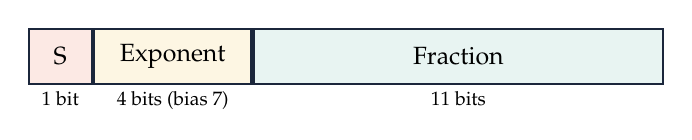
\begin{tikzpicture}[font=\small]
\node[draw=ink,thick,fill=rose,minimum width=8mm,minimum height=7mm] (s) {S};
\node[draw=ink,thick,fill=goldbg,minimum width=20mm,minimum height=7mm,right=0pt of s] (e) {Exponent};
\node[draw=ink,thick,fill=mist,minimum width=52mm,minimum height=7mm,right=0pt of e] (f) {Fraction};
\node[tk,below=1pt of s]{1 bit}; \node[tk,below=1pt of e]{4 bits (bias 7)}; \node[tk,below=1pt of f]{11 bits};
\end{tikzpicture}}
\sub{Conversion}
$0.75 = 0.11_2 = 1.1_2\times2^{-1}$: $E=-1+7=6$ $\Rightarrow$ \texttt{0 0110 10000000000} $=\hex{3400}$. \quad
$1.25 = 1.01_2\times2^{0}$: $E=7$ $\Rightarrow$ \texttt{0 0111 01000000000} $=\hex{3A00}$.

\sub{Addition (align, add, normalize, round)}
\fig{\small\renewcommand{\arraystretch}{1.25}
\begin{tabular}{lccc}
\toprule
Step & Exponent field & Significand (hidden bit shown) & Fraction field\\
\midrule
$0.75$ & \texttt{0110} ($-1$) & \texttt{1.10000000000} & \texttt{10000000000}\\
$1.25$ & \texttt{0111} ($0$) & \texttt{1.01000000000} & \texttt{01000000000}\\
\midrule
1. Align: $7-6=1$, shift $0.75$ right 1 & \texttt{0111} & \texttt{0.11000000000} & \texttt{11000000000}\\
2. Add significands & \texttt{0111} & \begin{tabular}[t]{@{}r@{}}\texttt{0.11000000000}\\ $+$\,\texttt{1.01000000000}\\ $=$\,\texttt{10.00000000000}\end{tabular} & ---\\
3. Normalize: shift right 1, $E+1$ & \texttt{1000} ($+1$) & \texttt{1.00000000000} & \texttt{00000000000}\\
\quad over/underflow? & \multicolumn{3}{l}{$1\le E=8\le14$ $\Rightarrow$ none}\\
4. Round (bit shifted out $=0$) & \texttt{1000} & \texttt{1.00000000000} & \texttt{00000000000}\\
\bottomrule
\end{tabular}}
\ans{$0.75+1.25 = 1.0_2\times2^{1} = 2.0$, \ stored as \texttt{0 1000 00000000000} $=\hex{4000}$.}
\end{solution}

%---------------------------------------------------------------- AR21
\begin{question}{2017--2018 \textbullet\ Q5(c)}{CSE 305 \textbullet\ 23/09/2018 \textbullet\ AR21}{5}
Determine the decimal value of the floating point represented by the hexadecimal value $(\texttt{7F80 0005})_{hex}$ according to IEEE 754 single precision floating point format.
\end{question}
\begin{solution}
Split the 32 bits into $S$ (1) $|$ $E$ (8) $|$ $F$ (23). If $1\le E\le254$ the value is $(-1)^S(1+F/2^{23})\,2^{E-127}$; $E=255$ is reserved: $F=0\Rightarrow\pm\infty$, $F\ne0\Rightarrow$ NaN.
\fig{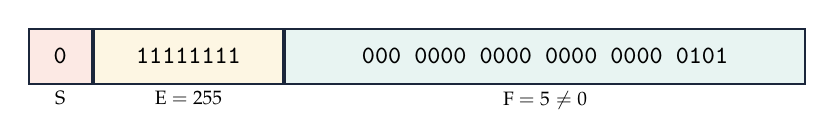
\begin{tikzpicture}[font=\small\ttfamily]
\node[draw=ink,thick,fill=rose,minimum width=8mm,minimum height=7mm] (s) {0};
\node[draw=ink,thick,fill=goldbg,minimum width=24mm,minimum height=7mm,right=0pt of s] (e) {11111111};
\node[draw=ink,thick,fill=mist,minimum width=66mm,minimum height=7mm,right=0pt of e] (f) {000 0000 0000 0000 0000 0101};
\node[tk,below=1pt of s]{S}; \node[tk,below=1pt of e]{E $=255$}; \node[tk,below=1pt of f]{F $=5\ne0$};
\end{tikzpicture}}
$\texttt{7F800005}=\texttt{0111\,1111\,1000\,0000\,0000\,0000\,0000\,0101}$: $S=0$, $E=\texttt{11111111}=255$ (reserved), $F=5\ne0$.
\ans{$(\texttt{7F800005})_{16}$ is \textbf{NaN} (Not-a-Number) --- it has no decimal value. (With the fraction MSB $=0$ it is a \emph{signalling} NaN.)}
\end{solution}

%---------------------------------------------------------------- AR22
\begin{question}{2017--2018 \textbullet\ Q8(a)}{CSE 305 \textbullet\ 23/09/2018 \textbullet\ AR22}{15}
Suppose you have a 4-bit ALU and you are required to perform a division operation, where the dividend is \texttt{11010101} and the divisor is \texttt{1011}. Show the division process step by step along with value of each relevant register at every step.
\end{question}
\begin{solution}
\sub{Hardware and algorithm: the Optimized Divider (slides)}
With a 4-bit ALU, $n=4$: a 4-bit \textbf{Divisor} register and an 8-bit \textbf{Remainder} register (left half Rem$_{hi}$, right half Rem$_{lo}$). There is no Quotient register; quotient bits enter at the right end of the Remainder.
\textbf{0.}~Remainder $\leftarrow$ dividend, shift Remainder left 1. Repeat $n$ times: \textbf{1.}~Rem$_{hi}\leftarrow$ Rem$_{hi}-$Divisor; \textbf{2a.}~if $\ge0$: shift Remainder left, new rightmost bit $=1$; \textbf{2b.}~if $<0$: restore (Rem$_{hi}+$Divisor), shift Remainder left, new rightmost bit $=0$. \textbf{3.}~Shift Rem$_{hi}$ right 1. Result: Rem$_{lo}=$ quotient, Rem$_{hi}=$ remainder.

\textbf{Why shift first?} The first quotient bit has weight $2^{n-1}$: it asks whether Divisor$\times2^{n-1}$ fits, i.e.\ it compares the Divisor with the dividend's top $n{+}1$ bits, which is what the left half holds after one left shift. Subtracting from the unshifted left half would test Divisor$\times2^{n}$, a quotient bit an $n$-bit quotient cannot have; if that test succeeds the division overflows (as happens here). The extra left shift is undone by the final right shift of Rem$_{hi}$.
\fig{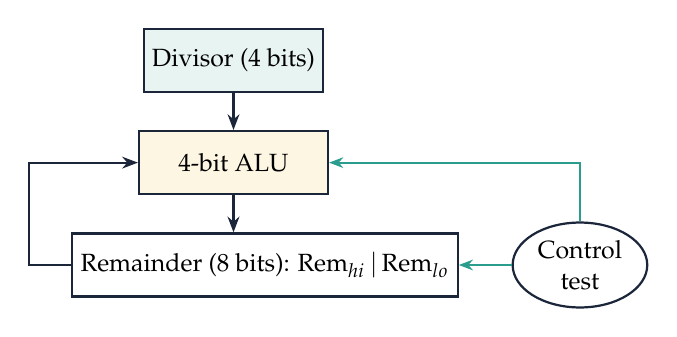
\begin{tikzpicture}[font=\small]
 \node[blkm,minimum width=20mm] (dv) at (0,0) {Divisor (4 bits)};
 \node[blkg,minimum width=24mm] (al) at (0,-1.3) {4-bit ALU};
 \node[blk,minimum width=46mm] (rm) at (0.4,-2.6) {Remainder (8 bits): Rem$_{hi}$\,$|$\,Rem$_{lo}$};
 \node[oval] (ct) at (4.4,-2.6) {Control\\test};
 \draw[wire] (dv) -- (al);
 \draw[wire] (al) -- ($(rm.north)+(-0.4,0)$);
 \draw[wire] ($(rm.west)$) -| (-2.6,-1.3) -- (al.west);
 \draw[ctl] (ct.west) -- (rm.east);
 \draw[ctl] (ct.north) |- (al.east);
\end{tikzpicture}}

\sub{Divide-overflow check}
The quotient can have only $n=4$ bits (it lives in Rem$_{lo}$). That works only if the dividend's left half is smaller than the divisor. Here Rem$_{hi}=\texttt{1101}=13 \ge \texttt{1011}=11$, so the true quotient $213\div11=19=\texttt{10011}_2$ needs 5 bits: this is a \key{divide overflow}. Real hardware checks Rem$_{hi}\ge$ Divisor before starting and signals overflow. Below the 4-bit trace is shown as asked, and then the same algorithm on a 5-bit ALU, which gives the correct result.

\sub{(i) Strict 4-bit trace: $\texttt{11010101}_2 \div \texttt{1011}_2$}
The first left shift pushes the dividend's leading 1 out of the 8-bit register, so the hardware is already working on the wrong number. Changed values are in \textcolor{coral}{\textbf{coral}}; a negative difference is signalled by the ALU's borrow.
\fig{\footnotesize\setlength{\tabcolsep}{4pt}\begin{tabular}{c>{\raggedright\arraybackslash}p{50mm}ccc}
\toprule
Iter. & Step & Divisor & Remainder (Rem$_{hi}$\,$|$\,Rem$_{lo}$) & sign\\
\midrule
0 & Initial values & \texttt{1011} & \texttt{1101}\,$|$\,\texttt{0101} & \\
 & Shift Rem left 1 (MSB 1 lost) & \texttt{1011} & \textcolor{coral}{\textbf{\texttt{1010}}}\,$|$\,\textcolor{coral}{\textbf{\texttt{1010}}} & \\
\midrule
1 & 1: Rem$_{hi}$ $\leftarrow$ Rem$_{hi}-$Div & \texttt{1011} & \textcolor{coral}{\textbf{\texttt{1111}}}\,$|$\,\texttt{1010} & $<0$\\
 & 2b: Rem$<$0: $+$Div, sll Rem, Rem$_0{=}0$ & \texttt{1011} & \textcolor{coral}{\textbf{\texttt{0101}}}\,$|$\,\textcolor{coral}{\textbf{\texttt{0100}}} & \\
\midrule
2 & 1: Rem$_{hi}$ $\leftarrow$ Rem$_{hi}-$Div & \texttt{1011} & \textcolor{coral}{\textbf{\texttt{1010}}}\,$|$\,\texttt{0100} & $<0$\\
 & 2b: Rem$<$0: $+$Div, sll Rem, Rem$_0{=}0$ & \texttt{1011} & \textcolor{coral}{\textbf{\texttt{1010}}}\,$|$\,\textcolor{coral}{\textbf{\texttt{1000}}} & \\
\bottomrule
\end{tabular}}
\fig{\footnotesize\setlength{\tabcolsep}{4pt}\begin{tabular}{c>{\raggedright\arraybackslash}p{50mm}ccc}
\toprule
Iter. & Step & Divisor & Remainder (Rem$_{hi}$\,$|$\,Rem$_{lo}$) & sign \ \textit{(cont.)}\\
\midrule
3 & 1: Rem$_{hi}$ $\leftarrow$ Rem$_{hi}-$Div & \texttt{1011} & \textcolor{coral}{\textbf{\texttt{1111}}}\,$|$\,\texttt{1000} & $<0$\\
 & 2b: Rem$<$0: $+$Div, sll Rem, Rem$_0{=}0$ & \texttt{1011} & \textcolor{coral}{\textbf{\texttt{0101}}}\,$|$\,\textcolor{coral}{\textbf{\texttt{0000}}} & \\
\midrule
4 & 1: Rem$_{hi}$ $\leftarrow$ Rem$_{hi}-$Div & \texttt{1011} & \textcolor{coral}{\textbf{\texttt{1010}}}\,$|$\,\texttt{0000} & $<0$\\
 & 2b: Rem$<$0: $+$Div, sll Rem, Rem$_0{=}0$ & \texttt{1011} & \textcolor{coral}{\textbf{\texttt{1010}}}\,$|$\,\textcolor{coral}{\textbf{\texttt{0000}}} & \\
\midrule
 & 3: Shift Rem$_{hi}$ right 1 & \texttt{1011} & \textcolor{coral}{\textbf{\texttt{0101}}}\,$|$\,\texttt{0000} & \\
\bottomrule
\end{tabular}}
The 4-bit hardware ends with quotient $\texttt{0000}$ and remainder $\texttt{0101}$, which is \textbf{wrong} ($11\times0+5\ne213$). This is the divide overflow: an $n$-bit divider cannot produce an $(n{+}1)$-bit quotient.

\sub{(ii) Same algorithm on a 5-bit ALU (correct result)}
With $n=5$ the dividend is $\texttt{00\,1101\,0101}$ (10-bit Remainder) and the Divisor is $\texttt{01011}$; now Rem$_{hi}=\texttt{00110}<\texttt{01011}$, so no overflow.
\fig{\footnotesize\setlength{\tabcolsep}{4pt}\begin{tabular}{c>{\raggedright\arraybackslash}p{50mm}ccc}
\toprule
Iter. & Step & Divisor & Remainder (Rem$_{hi}$\,$|$\,Rem$_{lo}$) & sign\\
\midrule
0 & Initial values & \texttt{01011} & \texttt{00110}\,$|$\,\texttt{10101} & \\
 & Shift Rem left 1 & \texttt{01011} & \textcolor{coral}{\textbf{\texttt{01101}}}\,$|$\,\textcolor{coral}{\textbf{\texttt{01010}}} & \\
\midrule
1 & 1: Rem$_{hi}$ $\leftarrow$ Rem$_{hi}-$Div & \texttt{01011} & \textcolor{coral}{\textbf{\texttt{00010}}}\,$|$\,\texttt{01010} & $\ge 0$\\
 & 2a: Rem$\ge$0: sll Rem, Rem$_0{=}1$ & \texttt{01011} & \textcolor{coral}{\textbf{\texttt{00100}}}\,$|$\,\textcolor{coral}{\textbf{\texttt{10101}}} & \\
\midrule
2 & 1: Rem$_{hi}$ $\leftarrow$ Rem$_{hi}-$Div & \texttt{01011} & \textcolor{coral}{\textbf{\texttt{11001}}}\,$|$\,\texttt{10101} & $<0$\\
 & 2b: Rem$<$0: $+$Div, sll Rem, Rem$_0{=}0$ & \texttt{01011} & \textcolor{coral}{\textbf{\texttt{01001}}}\,$|$\,\textcolor{coral}{\textbf{\texttt{01010}}} & \\
\midrule
3 & 1: Rem$_{hi}$ $\leftarrow$ Rem$_{hi}-$Div & \texttt{01011} & \textcolor{coral}{\textbf{\texttt{11110}}}\,$|$\,\texttt{01010} & $<0$\\
 & 2b: Rem$<$0: $+$Div, sll Rem, Rem$_0{=}0$ & \texttt{01011} & \textcolor{coral}{\textbf{\texttt{10010}}}\,$|$\,\textcolor{coral}{\textbf{\texttt{10100}}} & \\
\bottomrule
\end{tabular}}
\fig{\footnotesize\setlength{\tabcolsep}{4pt}\begin{tabular}{c>{\raggedright\arraybackslash}p{50mm}ccc}
\toprule
Iter. & Step & Divisor & Remainder (Rem$_{hi}$\,$|$\,Rem$_{lo}$) & sign \ \textit{(cont.)}\\
\midrule
4 & 1: Rem$_{hi}$ $\leftarrow$ Rem$_{hi}-$Div & \texttt{01011} & \textcolor{coral}{\textbf{\texttt{00111}}}\,$|$\,\texttt{10100} & $\ge 0$\\
 & 2a: Rem$\ge$0: sll Rem, Rem$_0{=}1$ & \texttt{01011} & \textcolor{coral}{\textbf{\texttt{01111}}}\,$|$\,\textcolor{coral}{\textbf{\texttt{01001}}} & \\
\midrule
5 & 1: Rem$_{hi}$ $\leftarrow$ Rem$_{hi}-$Div & \texttt{01011} & \textcolor{coral}{\textbf{\texttt{00100}}}\,$|$\,\texttt{01001} & $\ge 0$\\
 & 2a: Rem$\ge$0: sll Rem, Rem$_0{=}1$ & \texttt{01011} & \textcolor{coral}{\textbf{\texttt{01000}}}\,$|$\,\textcolor{coral}{\textbf{\texttt{10011}}} & \\
\midrule
 & 3: Shift Rem$_{hi}$ right 1 & \texttt{01011} & \textcolor{coral}{\textbf{\texttt{00100}}}\,$|$\,\texttt{10011} & \\
\bottomrule
\end{tabular}}
\ans{The 4-bit divider overflows (quotient needs 5 bits) and gives a wrong result. With a 5-bit ALU: Quotient $=\texttt{10011}_2=19$, Remainder $=\texttt{00100}_2=4$. \ Check: $11\times19+4=213$ \ok}
\end{solution}

%---------------------------------------------------------------- AR23
\begin{question}{2017--2018 \textbullet\ Q8(b)}{CSE 305 \textbullet\ 23/09/2018 \textbullet\ AR23}{10}
Write down the equivalent MIPS assembly code for the following function, written in C programming language. Assume appropriate registers for the variables.
\begin{ccode}
float convert (float cels)
{
    float ferh = (9.0 * cels) / 5.0;
    ferh = ferh + 32.0;
    return ferh;
}
\end{ccode}
\end{question}
\begin{solution}
\sub{Rules used (slides: FP instructions in MIPS, \texttt{f2c} example)}
FP registers \reg{f0}--\reg{f31} (doubles in even/odd pairs); single ops \ins{.s}, double ops \ins{.d}; loads \ins{lwc1} (single) / \ins{ldc1} (double); conversions \ins{cvt.d.s} / \ins{cvt.s.d}.
Convention: argument \texttt{cels} in \reg{f12}, result in \reg{f0}, constants in the global data area (offsets from \reg{gp}).

\sub{Exact C semantics}
In C the literals \texttt{9.0}, \texttt{5.0}, \texttt{32.0} are \emph{double}, so \texttt{cels} is promoted, the arithmetic is double, and the value is converted back to float at each assignment to \texttt{ferh}:
\begin{mips}
convert:
      ldc1    $f16, const9($gp)   # $f16 = 9.0  (double constant)
      cvt.d.s $f18, $f12          # $f18 = (double) cels
      mul.d   $f16, $f16, $f18    # 9.0 * cels
      ldc1    $f18, const5($gp)   # $f18 = 5.0
      div.d   $f16, $f16, $f18    # (9.0*cels) / 5.0
      cvt.s.d $f0, $f16           # ferh = (float) result
      cvt.d.s $f16, $f0           # promote ferh for ferh + 32.0
      ldc1    $f18, const32($gp)  # $f18 = 32.0
      add.d   $f16, $f16, $f18    # ferh + 32.0 (double)
      cvt.s.d $f0, $f16           # ferh = (float) ..., return in $f0
      jr      $ra
\end{mips}
\sub{All-single version}
If the constants are stored as single-precision floats (as in the slides' \texttt{f2c} example, i.e.\ \texttt{9.0f} etc.), everything stays single and no conversions are needed:
\begin{mips}
convert:
      lwc1  $f16, const9($gp)     # 9.0f
      mul.s $f16, $f16, $f12      # 9.0 * cels
      lwc1  $f18, const5($gp)     # 5.0f
      div.s $f16, $f16, $f18      # ferh = (9.0*cels)/5.0
      lwc1  $f18, const32($gp)    # 32.0f
      add.s $f0, $f16, $f18       # ferh = ferh + 32.0 -> $f0
      jr    $ra
\end{mips}
\end{solution}

%---------------------------------------------------------------- AR24
\begin{question}{2016--2017 \textbullet\ Q7(b)}{CSE 305 \textbullet\ 02/08/2017 \textbullet\ AR24}{15}
Consider the following block diagram of a floating point addition hardware.

\fig{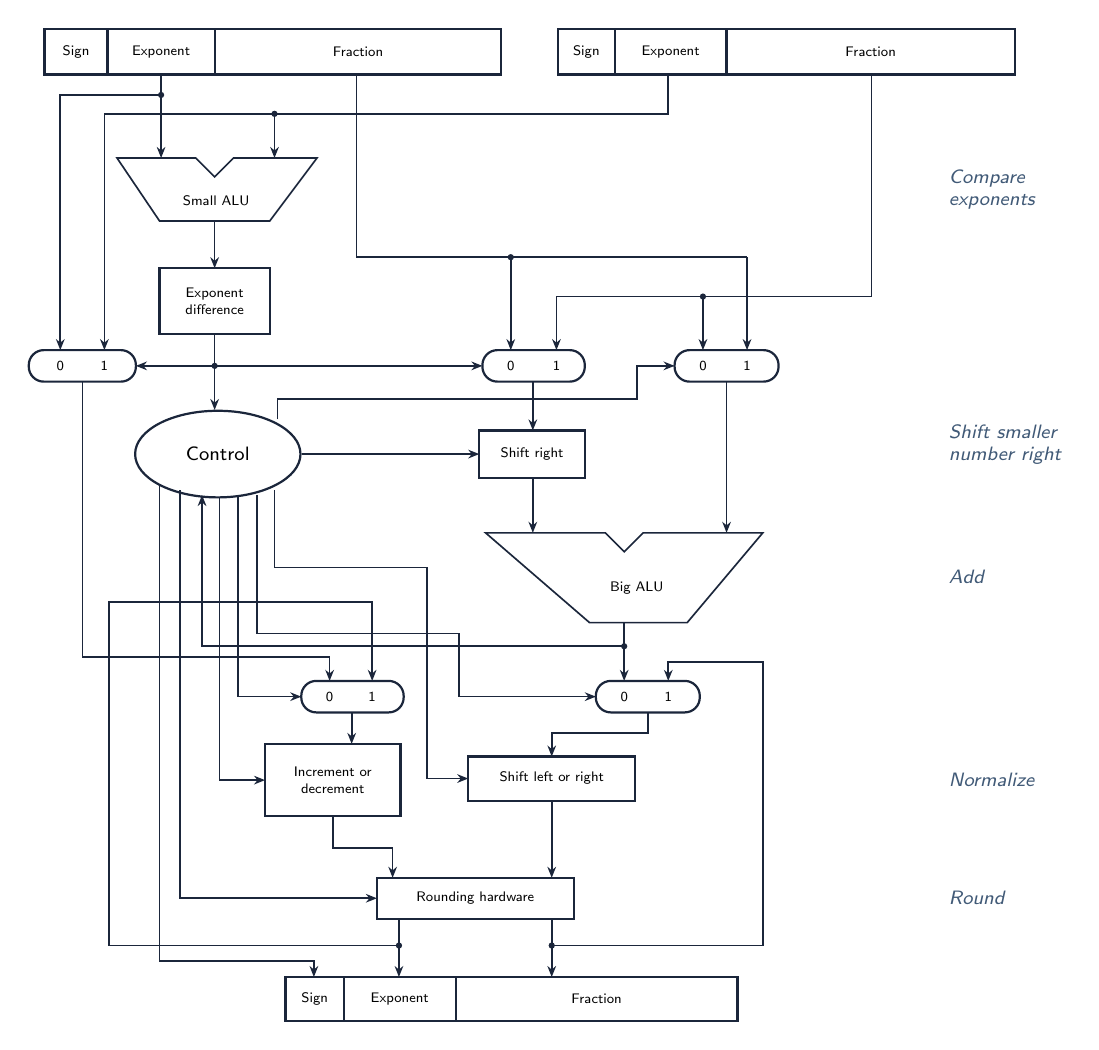
\begin{tikzpicture}[x=0.02cm,y=-0.02cm,font=\sffamily\scriptsize,
  w/.style={->,>={Stealth[length=1.4mm,width=1.1mm]},semithick,ink},
  l/.style={semithick,ink},
  bx/.style={draw=ink,thick,fill=white},
  hm/.style={draw=ink,thick,fill=white,rounded corners=1.9mm},
  dt/.style={circle,fill=ink,inner sep=0.8pt},
  lb/.style={font=\sffamily\tiny,inner sep=1pt},
  st/.style={font=\sffamily\scriptsize\itshape,text=inksoft,anchor=west,align=left}]
% ---------- operand registers
\draw[bx] (272,598) rectangle node[lb]{Sign} (312,627);
\draw[bx] (312,598) rectangle node[lb]{Exponent} (380,627);
\draw[bx] (380,598) rectangle node[lb]{Fraction} (562,627);
\draw[bx] (598,598) rectangle node[lb]{Sign} (634,627);
\draw[bx] (634,598) rectangle node[lb]{Exponent} (705,627);
\draw[bx] (705,598) rectangle node[lb]{Fraction} (888,627);
% ---------- compare exponents
\draw[l,fill=white] (318,680) -- (368,680) -- (380,692) -- (392,680) -- (445,680) -- (415,720) -- (345,720) -- cycle;
\node[lb] at (381,707) {Small ALU};
\draw[w] (346,627) -- (346,680); \node[dt] at (346,640) {};
\draw[w] (346,640) -- (282,640) -- (282,802);
\draw[l] (668,627) -- (668,652) -- (310,652); \node[dt] at (418,652) {};
\draw[w] (418,652) -- (418,680);
\draw[w] (310,652) -- (310,802);
\draw[bx] (345,750) rectangle node[lb,align=center]{Exponent\\difference} (415,792);
\draw[w] (380,720) -- (380,750);
\draw[w] (380,792) -- (380,840); \node[dt] at (380,812) {};
% ---------- the three upper muxes
\draw[hm] (262,802) rectangle (330,822); \node[lb] at (282,812) {0}; \node[lb] at (310,812) {1};
\draw[hm] (550,802) rectangle (615,822); \node[lb] at (568,812) {0}; \node[lb] at (597,812) {1};
\draw[hm] (672,802) rectangle (738,822); \node[lb] at (690,812) {0}; \node[lb] at (718,812) {1};
\draw[w] (380,812) -- (330,812);
\draw[w] (380,812) -- (550,812);
\draw[l] (470,627) -- (470,743) -- (718,743); \node[dt] at (568,743) {};
\draw[w] (718,743) -- (718,802);
\draw[w] (568,743) -- (568,802);
\draw[l] (797,627) -- (797,768) -- (597,768); \node[dt] at (690,768) {};
\draw[w] (597,768) -- (597,802);
\draw[w] (690,768) -- (690,802);
% ---------- shift smaller number right, add
\node[draw=ink,thick,fill=white,ellipse,minimum width=21mm,minimum height=11mm,inner sep=0pt] (ctl) at (382,868) {Control};
\draw[w] (420,846) -- (420,833) -- (648,833) -- (648,812) -- (672,812);
\draw[bx] (548,853) rectangle node[lb]{Shift right} (615,883);
\draw[w] (582,822) -- (582,853);
\draw[w] (ctl.east) -- (548,868);
\draw[l,fill=white] (552,918) -- (628,918) -- (640,930) -- (652,918) -- (728,918) -- (680,975) -- (618,975) -- cycle;
\node[lb] at (648,953) {Big ALU};
\draw[w] (582,883) -- (582,918);
\draw[w] (705,822) -- (705,918);
% ---------- normalize
\draw[hm] (435,1012) rectangle (500,1032); \node[lb] at (453,1022) {0}; \node[lb] at (480,1022) {1};
\draw[hm] (622,1012) rectangle (688,1032); \node[lb] at (640,1022) {0}; \node[lb] at (668,1022) {1};
\draw[l] (640,975) -- (640,990); \node[dt] at (640,990) {};
\draw[w] (640,990) -- (640,1012);
\draw[w] (640,990) -- (372,990) -- (372,894);
\draw[w] (296,822) -- (296,997) -- (453,997) -- (453,1012);
\draw[bx] (412,1052) rectangle node[lb,align=center]{Increment or\\decrement} (498,1098);
\draw[bx] (541,1060) rectangle node[lb]{Shift left or right} (647,1088);
\draw[w] (467,1032) -- (467,1052);
\draw[w] (655,1032) -- (655,1045) -- (594,1045) -- (594,1060);
\draw[w] (395,895) -- (395,1022) -- (435,1022);
\draw[w] (383,896) -- (383,1075) -- (412,1075);
\draw[w] (418,891) -- (418,940) -- (515,940) -- (515,1074) -- (541,1074);
\draw[w] (407,894) -- (407,982) -- (535,982) -- (535,1022) -- (622,1022);
% ---------- round
\draw[bx] (483,1137) rectangle node[lb]{Rounding hardware} (608,1163);
\draw[w] (455,1098) -- (455,1118) -- (493,1118) -- (493,1137);
\draw[w] (594,1088) -- (594,1137);
\draw[w] (358,891) -- (358,1150) -- (483,1150);
\draw[w] (497,1163) -- (497,1200); \node[dt] at (497,1180) {};
\draw[w] (594,1163) -- (594,1200); \node[dt] at (594,1180) {};
\draw[w] (497,1180) -- (313,1180) -- (313,962) -- (480,962) -- (480,1012);
\draw[w] (594,1180) -- (728,1180) -- (728,1000) -- (668,1000) -- (668,1012);
\draw[w] (345,888) -- (345,1190) -- (443,1190) -- (443,1200);
% ---------- result
\draw[bx] (425,1200) rectangle node[lb]{Sign} (462,1228);
\draw[bx] (462,1200) rectangle node[lb]{Exponent} (533,1228);
\draw[bx] (533,1200) rectangle node[lb]{Fraction} (712,1228);
% ---------- step labels
\node[st] at (840,700) {Compare\\exponents};
\node[st] at (840,862) {Shift smaller\\number right};
\node[st] at (840,946) {Add};
\node[st] at (840,1075) {Normalize};
\node[st] at (840,1150) {Round};
\end{tikzpicture}}
{\centering\small\itshape Block diagram of the floating-point addition hardware\par}

Using the given hardware, simulate the floating addition algorithm by filling up the following tables. The two numbers for addition are, $-(0.25)_{10}$ and $(0.625)_{10}$.

\begin{center}\renewcommand{\arraystretch}{1.6}
\begin{tabular}{lccc}
 & \fbox{\makebox[26mm]{$-(0.25)_{10}$}} & & \fbox{\makebox[26mm]{$(0.625)_{10}$}}\\
Binary & \fbox{\makebox[26mm]{\strut}} & & \fbox{\makebox[26mm]{\strut}}\\
Step1: Exponent Matching & \fbox{\makebox[26mm]{\strut}} & & \fbox{\makebox[26mm]{\strut}}\\
Step2: Significand Addition & & & \\
Step3: Normalization & \fbox{\makebox[26mm]{\strut}} & $=$ & \fbox{\makebox[26mm]{\strut}}\\
Step4: Rounding & \fbox{\makebox[26mm]{\strut}} & & \\
\end{tabular}\end{center}
\end{question}
\begin{solution}
\sub{Method}
The hardware does the four steps of FP addition: (1) the small ALU subtracts the exponents and the control shifts the significand of the number with the smaller exponent right by the difference; (2) the big ALU adds the signed significands; (3) the result is normalized (shift left/right with exponent decrement/increment) and checked for over/underflow; (4) the rounding hardware rounds (and renormalizes if needed). 4-bit significands are used, as in the slides.

\sub{Filled tables}
$-0.25 = -0.01_2 = -1.000_2\times2^{-2}$ (fields \texttt{1\,|\,01111101\,|\,000\ldots}) and
$0.625 = 0.101_2 = 1.010_2\times2^{-1}$ (fields \texttt{0\,|\,01111110\,|\,010\ldots}).
\begin{center}\small\renewcommand{\arraystretch}{1.35}
\begin{tabular}{lccc}
\toprule
 & $-(0.25)_{10}$ & & $(0.625)_{10}$\\
\midrule
Binary & $-1.000\times2^{-2}$ & & $1.010\times2^{-1}$\\
Step1: Exponent matching & $-0.100\times2^{-1}$ & & $1.010\times2^{-1}$\\
Step2: Significand addition & \multicolumn{3}{c}{$1.010\times2^{-1} + (-0.100\times2^{-1}) = 0.110\times2^{-1}$}\\
Step3: Normalization & $0.110\times2^{-1}$ & $=$ & $1.100\times2^{-2}$\\
Step4: Rounding & $1.100\times2^{-2}$ & & (already fits; $=0.375$)\\
\bottomrule
\end{tabular}\end{center}
\sub{How the hardware does it}
\fig{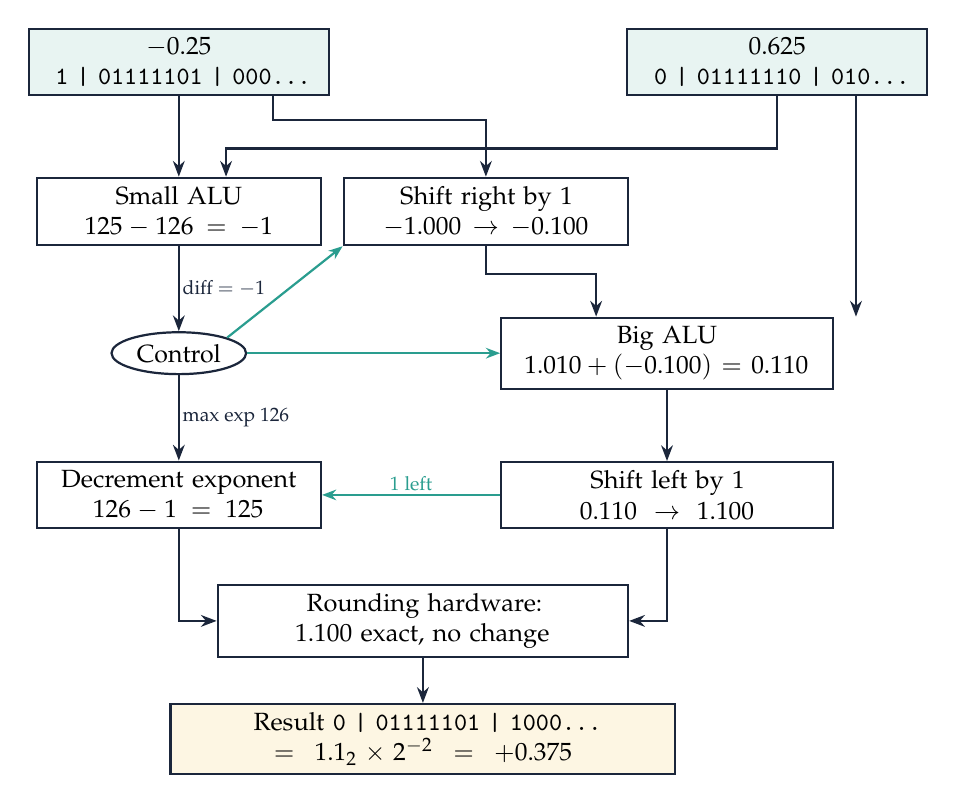
\begin{tikzpicture}[font=\small]
\node[blkm,text width=36mm] (A) at (0,0) {$-0.25$\\\texttt{1 | 01111101 | 000\ldots}};
\node[blkm,text width=36mm] (B) at (7.6,0) {$0.625$\\\texttt{0 | 01111110 | 010\ldots}};
\node[blk,text width=34mm] (sa) at (0,-1.9) {Small ALU\\$125-126=-1$};
\node[oval] (ct) at (0,-3.7) {Control};
\node[blk,text width=34mm] (sh) at (3.9,-1.9) {Shift right by 1\\$-1.000\to-0.100$};
\node[blk,text width=40mm] (big) at (6.2,-3.7) {Big ALU\\$1.010+(-0.100)=0.110$};
\node[blk,text width=34mm] (id) at (0,-5.5) {Decrement exponent\\$126-1=125$};
\node[blk,text width=40mm] (sl) at (6.2,-5.5) {Shift left by 1\\$0.110\to1.100$};
\node[blk,text width=50mm] (rd) at (3.1,-7.1) {Rounding hardware: $1.100$ exact, no change};
\node[blkg,text width=62mm] (out) at (3.1,-8.6) {Result \texttt{0 | 01111101 | 1000\ldots} $=1.1_2\times2^{-2}=+0.375$};
\draw[wire] (A.south)--(sa.north);
\draw[wire] (B.south) -- (B.south |- 0,-1.1) -| ([xshift=6mm]sa.north);
\draw[wire] ([xshift=12mm]A.south) |- ++(0,-0.3) -| (sh.north);
\draw[wire] (sh.south) |- ++(0,-0.35) -| ([xshift=-9mm]big.north);
\draw[wire] ([xshift=10mm]B.south)--([xshift=10mm]B.south |- big.north);
\draw[wire] (sa)--node[tk,right]{diff $=-1$}(ct);
\draw[ctl] (ct.north east)--(sh.south west);
\draw[ctl] (ct)--(big);
\draw[wire] (ct)--node[tk,right]{max exp 126}(id);
\draw[wire] (big)--(sl);
\draw[ctl] (sl)--node[tk,above]{1 left}(id);
\draw[wire] (id.south) |- (rd.west);
\draw[wire] (sl.south) |- (rd.east);
\draw[wire] (rd)--(out);
\end{tikzpicture}}
Exponent after normalization $=-2$ (biased 125), inside $[-126,127]$: no overflow/underflow, and rounding leaves it normalized.
\ans{$-0.25+0.625 = 1.100_2\times2^{-2} = +0.375$; single precision \texttt{0 01111101 10000000000000000000000} $=\hex{3EC00000}$.}
\end{solution}

%---------------------------------------------------------------- AR25
\repeated{2}
\begin{question}{2016--2017 \textbullet\ Q8(a)}{CSE 305 \textbullet\ 02/08/2017 \textbullet\ AR25}{5 + 5}
The following table illustrates the various combinations of two operands for binary addition-subtraction. Please identify the overflow conditions in that table. Then, formulate the overflow boolean variable as a logical function of various input variables (You don't need to simplify the function).
\begin{center}\begin{minipage}[c]{0.3\linewidth}\centering\small
\begin{tabular}{|c|c|c|c|c|}
\hline
$O$ & $S_A$ & $S_B$ & $S_R$ & $V$\\\hline
0&0&0&&\\\hline 0&0&1&&\\\hline 0&1&0&&\\\hline 0&1&1&&\\\hline
1&0&0&&\\\hline 1&0&1&&\\\hline 1&1&0&&\\\hline 1&1&1&&\\\hline
\end{tabular}\end{minipage}\hfill
\begin{minipage}[c]{0.62\linewidth}\small
Here,\\[2pt]
Operation, $O=\begin{cases}0, & A+B\\ 1, & A-B\end{cases}$\\[4pt]
Sign bit of Operand A, $S_A=\begin{cases}0, & A\ge0\\ 1, & A<0\end{cases}$\\[4pt]
Sign bit of Operand B, $S_B=\begin{cases}0, & B\ge0\\ 1, & B<0\end{cases}$\\[4pt]
Sign bit of Result R, $S_R=\begin{cases}0, & R\ge0\\ 1, & R<0\end{cases}$\\[4pt]
Overflow, $V=\begin{cases}1, & \text{Overflow occurred}\\ 0, & \text{No overflow possible}\end{cases}$
\end{minipage}\end{center}
\end{question}
\begin{question}{2014--2015 \textbullet\ Q8(a)}{CSE 305 \textbullet\ 26/01/2016 \textbullet\ AR25}{8 + 4}
The following table illustrates the various combinations of two operands for binary addition-subtraction. Please identify the overflow conditions in that table. Then, formulate the overflow boolean variable as a logical function of various input variables (You don't need to simplify the function).

\begin{center}\begin{minipage}[c]{0.3\linewidth}\centering\small
\begin{tabular}{|c|c|c|c|c|}
\hline
$O$ & $S_A$ & $S_B$ & $S_R$ & $V$\\\hline
0&0&0&&\\\hline 0&0&1&&\\\hline 0&1&0&&\\\hline 0&1&1&&\\\hline
1&0&0&&\\\hline 1&0&1&&\\\hline 1&1&0&&\\\hline 1&1&1&&\\\hline
\end{tabular}\end{minipage}\hfill
\begin{minipage}[c]{0.62\linewidth}\small
Here,\\[2pt]
Operation, $O=\begin{cases}0, & A+B\\ 1, & A-B\end{cases}$\\[4pt]
Sign bit if Operand A, $S_A=\begin{cases}0, & A\ge0\\ 1, & A<0\end{cases}$\\[4pt]
Sign bit of Operand B, $S_B=\begin{cases}0, & B\ge0\\ 1, & B<0\end{cases}$\\[4pt]
Sign bit of Result R, $S_R=\begin{cases}0, & R\ge0\\ 1, & R<0\end{cases}$\\[4pt]
Overflow, $V=\begin{cases}0, & \text{Overflow occured}\\ 1, & \text{No overflow possible}\end{cases}$
\end{minipage}\end{center}
\end{question}
\begin{solution}
\sub{Identifying overflow}
Overflow is possible only when the \emph{effective} operands have the same sign: $A+B$ with $S_A=S_B$, or $A-B$ (i.e.\ $A+(-B)$) with $S_A\ne S_B$. It then occurs when the result sign $S_R$ differs from $S_A$ (slides: $+$ve $+$ $+$ve $\to$ sign 1, $-$ve $+$ $-$ve $\to$ sign 0, $+$ve $-$ $-$ve $\to$ sign 1, $-$ve $-$ $+$ve $\to$ sign 0). For the other rows overflow is impossible whatever $S_R$ is.
\begin{center}\small\begin{tabular}{ccc|c|c|l}
\toprule
$O$ & $S_A$ & $S_B$ & $S_R$ & $V$ & Meaning\\
\midrule
0&0&0& \textcolor{coral}{\textbf{1}} & \textcolor{coral}{\textbf{1}} & $(+)+(+)$ gives $-$: overflow\\
0&0&1& x & 0 & $(+)+(-)$: no overflow possible\\
0&1&0& x & 0 & $(-)+(+)$: no overflow possible\\
0&1&1& \textcolor{coral}{\textbf{0}} & \textcolor{coral}{\textbf{1}} & $(-)+(-)$ gives $+$: overflow\\
1&0&0& x & 0 & $(+)-(+)$: no overflow possible\\
1&0&1& \textcolor{coral}{\textbf{1}} & \textcolor{coral}{\textbf{1}} & $(+)-(-)$ gives $-$: overflow\\
1&1&0& \textcolor{coral}{\textbf{0}} & \textcolor{coral}{\textbf{1}} & $(-)-(+)$ gives $+$: overflow\\
1&1&1& x & 0 & $(-)-(-)$: no overflow possible\\
\bottomrule
\end{tabular}\end{center}
(x $=$ either value; with the opposite $S_R$ in the four overflow rows, $V=0$.)

\sub{Overflow function (sum of the four minterms in $O, S_A, S_B, S_R$)}
\[ V = \overline{O}\,\overline{S_A}\,\overline{S_B}\,S_R \;+\; \overline{O}\,S_A\,S_B\,\overline{S_R} \;+\; O\,\overline{S_A}\,S_B\,S_R \;+\; O\,S_A\,\overline{S_B}\,\overline{S_R} \]
(Optionally simplified: $V = \overline{S_A\oplus S_B\oplus O}\cdot(S_A\oplus S_R)$ --- the effective signs agree and the result sign differs.)

\begin{note}\textbf{2014--2015 card:} the scan defines $V=0$ for ``overflow occurred'' and $V=1$ for ``no overflow possible'' --- the reverse of the 2016--17 paper and of the usual convention (probably a misprint). Under the definition exactly as printed, the $V$ column above is simply complemented (1 in the four ``no overflow'' rows, 0 in the overflow rows), and
$V_{\text{printed}} = \overline{\,\overline{O}\,\overline{S_A}\,\overline{S_B}\,S_R + \overline{O}\,S_A\,S_B\,\overline{S_R} + O\,\overline{S_A}\,S_B\,S_R + O\,S_A\,\overline{S_B}\,\overline{S_R}\,}$.\end{note}
\end{solution}

%---------------------------------------------------------------- AR26
\begin{question}{2016--2017 \textbullet\ Q8(c)}{CSE 305 \textbullet\ 02/08/2017 \textbullet\ AR26}{15}
Consider the following multiplication hardware.
\fig{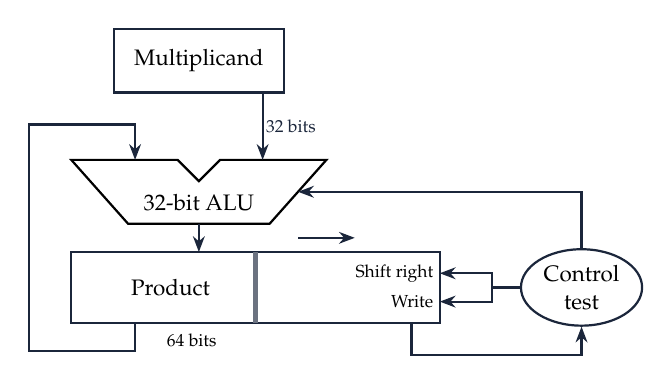
\begin{tikzpicture}[font=\small,scale=0.9,transform shape]
\node[blk,minimum width=24mm,minimum height=9mm] (mc) at (0,3) {Multiplicand};
\draw[thick,fill=white] (-1.8,1.6) -- (-0.3,1.6) -- (0,1.3) -- (0.3,1.6) -- (1.8,1.6) -- (1.0,0.7) -- (-1.0,0.7) -- cycle;
\node at (0,1.0) {32-bit ALU};
\draw[wire] (0.9,2.55) -- node[right,tk]{32 bits} (0.9,1.6);
\node[blk,minimum width=52mm,minimum height=10mm] (pr) at (0.8,-0.2) {};
\node at (-0.4,-0.2) {Product};
\draw[slate,line width=2pt] (0.8,-0.7) -- (0.8,0.3);
\node[tk,anchor=east] at (3.35,0.0) {Shift right};
\node[tk,anchor=east] at (3.35,-0.4) {Write};
\draw[wire] (1.4,0.5) -- (2.2,0.5);
\draw[wire] (0,0.7) -- (0,0.3);
\draw[wire] (-0.9,-0.7) -- (-0.9,-1.1) -- (-2.4,-1.1) -- (-2.4,2.1) -- (-0.9,2.1) -- (-0.9,1.6);
\node[tk] at (-0.1,-0.95) {64 bits};
\node[oval] (ct) at (5.4,-0.2) {Control\\test};
\draw[wire] (ct.west) -- ++(-0.4,0) |- (3.4,0.0);
\draw[wire] (ct.west) -- ++(-0.4,0) |- (3.4,-0.4);
\draw[wire] (ct.north) |- (1.4,1.15);
\draw[wire] (3.0,-0.7) -- (3.0,-1.15) -| (ct.south);
\end{tikzpicture}}
Using the given hardware, simulate the unsigned multiplication algorithm by filling up the following tables for Multiplicand, 0110 and Multiplier, 0110.
\fig{\begin{tikzpicture}[x=5.5mm,y=5.5mm]
\foreach \y in {0,-2.2,-3.2,-5.4,-6.4,-8.6,-9.6,-11.8,-12.8} {\foreach \k in {0,...,7} {\draw[thick] (\k,\y) rectangle ++(1,0.8);}}
\foreach \y/\n in {-1/1,-4.2/2,-7.4/3,-10.6/4} {\node[font=\small] at (-0.8,\y+0.4) {\n}; \foreach \k in {0,...,3} {\draw[thick] (\k,\y) rectangle ++(1,0.8);}}
\foreach \y in {-1.5,-4.7,-7.9,-11.1} {\draw (-1.5,\y) -- (9,\y);}
\end{tikzpicture}}
\end{question}
\begin{solution}
\sub{Algorithm for the given (refined) hardware}
The 64-bit Product register starts with 0 in its left half and the multiplier in its right half. Each of the $n$ iterations (here $n=4$) does two things:
\begin{enumerate}
\item If Product0 $=1$, add the Multiplicand to the left half of the Product and write the result back into the left half.
\item Shift the Product register right 1 bit; the ALU carry-out enters at the MSB.
\end{enumerate}
Expected result: $6\times6=36=0010\,0100_2$.
\fig{\small\begin{tabular}{clcc}\toprule
Iteration & Step & Multiplicand & Product\\\midrule
0 & Initial values & 0110 & 0000 0110\\\midrule
1 & 1: Prod0 $=0\Rightarrow$ no operation & 0110 & 0000 011\textbf{0}\\
  & 2: Shift right Product & 0110 & 0000 0011\\\midrule
2 & 1a: Prod0 $=1\Rightarrow$ $0000+0110$ & 0110 & 0110 001\textbf{1}\\
  & 2: Shift right Product & 0110 & 0011 0001\\\midrule
3 & 1a: Prod0 $=1\Rightarrow$ $0011+0110$ & 0110 & 1001 000\textbf{1}\\
  & 2: Shift right Product & 0110 & 0100 1000\\\midrule
4 & 1: Prod0 $=0\Rightarrow$ no operation & 0110 & 0100 100\textbf{0}\\
  & 2: Shift right Product & 0110 & \textbf{0010 0100}\\\bottomrule
\end{tabular}}
The same values written into the answer form. The 8-box rows are the Product register; the 4-box rows are the Multiplicand used in iteration $k$:
\fig{\begin{tikzpicture}[x=5.5mm,y=5.5mm,font=\small]
\foreach \y/\bits/\t in {0/{0,0,0,0,0,1,1,0}/{initial Product},
 -2.2/{0,0,0,0,0,1,1,0}/{it.\,1: Prod0$=0$, no add},-3.2/{0,0,0,0,0,0,1,1}/{it.\,1: shift right},
 -5.4/{0,1,1,0,0,0,1,1}/{it.\,2: add Mcand},-6.4/{0,0,1,1,0,0,0,1}/{it.\,2: shift right},
 -8.6/{1,0,0,1,0,0,0,1}/{it.\,3: add Mcand},-9.6/{0,1,0,0,1,0,0,0}/{it.\,3: shift right},
 -11.8/{0,1,0,0,1,0,0,0}/{it.\,4: Prod0$=0$, no add},-12.8/{0,0,1,0,0,1,0,0}/{it.\,4: shift right $\Rightarrow$ 36}}
 {\foreach \b [count=\k from 0] in \bits {\draw[thick] (\k,\y) rectangle ++(1,0.8); \node[font=\small\ttfamily] at (\k+0.5,\y+0.4) {\b};}
  \node[tk,anchor=west] at (8.3,\y+0.4) {\t};}
\foreach \y/\n in {-1/1,-4.2/2,-7.4/3,-10.6/4} {\node[font=\small] at (-0.8,\y+0.4) {\n};
  \foreach \b [count=\k from 0] in {0,1,1,0} {\draw[thick] (\k,\y) rectangle ++(1,0.8); \node[font=\small\ttfamily] at (\k+0.5,\y+0.4) {\b};}
  \node[tk,anchor=west] at (4.3,\y+0.4) {Multiplicand};}
\foreach \y in {-1.5,-4.7,-7.9,-11.1} {\draw[slate] (-1.5,\y) -- (15,\y);}
\end{tikzpicture}}
\ans{$0110\times0110 = 0010\,0100_2 = 36_{10}$.}
\begin{note}The answer form in the scan has no row labels. We read it as: the initial Product, then for each iteration $k$ the Multiplicand box ``$k$'', followed by the Product after step 1 (add or no-op) and after the right shift.\end{note}
\end{solution}

%---------------------------------------------------------------- AR27
\begin{question}{2013--2014 \textbullet\ Q3(b)}{CSE 305 \textbullet\ 05/07/2015 \textbullet\ AR27}{10}
Show the IEEE 754 binary representation of the number $-0.75_{\text{ten}}$ in single precision.
\end{question}
\begin{solution}
\begin{enumerate}[label=\textbf{\arabic*.}]
\item Binary: $0.75 = 0.5+0.25 = 0.11_2$, so $-0.75 = -0.11_2$.
\item Normalize: $-0.11_2 = (-1)^1\times1.1_2\times2^{-1}$.
\item Sign $S=1$; Fraction $F = \texttt{1000\ldots0}$ (the leading 1 is hidden); Exponent $E = -1 + 127 = 126 = \texttt{01111110}_2$.
\end{enumerate}
\fig{\begin{tikzpicture}[font=\small\ttfamily]
\node[draw=ink,thick,fill=rose,minimum width=8mm,minimum height=7mm] (s) {1};
\node[draw=ink,thick,fill=goldbg,minimum width=24mm,minimum height=7mm,right=0pt of s] (e) {01111110};
\node[draw=ink,thick,fill=mist,minimum width=66mm,minimum height=7mm,right=0pt of e] (f) {100 0000 0000 0000 0000 0000};
\node[tk,below=1pt of s]{S}; \node[tk,below=1pt of e]{E: bits 30--23}; \node[tk,below=1pt of f]{F: bits 22--0};
\end{tikzpicture}}
Check: $(-1)^1\times(1+0.5)\times2^{126-127} = -1.5\times0.5 = -0.75$ \ok
\ans{$-0.75 = \texttt{1 01111110 10000000000000000000000}_2 = \hex{BF400000}$.}
\end{solution}

%---------------------------------------------------------------- AR28
\begin{question}{2012--2013 \textbullet\ Q8(b)}{CSE 305 \textbullet\ 10/05/2014 \textbullet\ AR28}{12}
Draw the flowchart showing the execution steps of the division operation for the division hardware organization given below:
\fig{\begin{tikzpicture}[font=\small]
\node[blk,minimum width=22mm] (dv) at (2.3,1.3) {Divisor};
\draw[thick,ink,fill=white] (0,0)--(1.25,0)--(1.5,-0.3)--(1.75,0)--(3,0)--(2.3,-0.85)--(0.7,-0.85)--cycle;
\node at (1.5,-0.6) {32-bit ALU};
\draw[wire] (dv.south)--node[tk,right]{32 bits}(2.3,0);
\node[blk,minimum width=50mm,minimum height=10mm] (rm) at (1.6,-2.2) {};
\node at (1.0,-2.2) {Remainder};
\node[tk,align=right,anchor=east] at (4.05,-2.2) {Shift right\\Shift left\\Write};
\draw[<->,thick,ink] (1.1,-1.45)--(1.9,-1.45);
\node[oval] (ct) at (6.1,-2.2) {Control\\test};
\draw[wire] (1.5,-0.85)--(1.5,-1.7);
\draw[ctl] (ct.west)--(4.1,-2.2);
\draw[ctl] (ct.north west)++(0,0.02) -- (4.1,-1.95);
\draw[ctl] (ct.south west)++(0,-0.02) -- (4.1,-2.45);
\draw[ctl] (ct.north) |- (2.65,-0.42);
\draw[wire] (0.6,-2.7)--(0.6,-3.15) -- (-1.2,-3.15) -- (-1.2,0.45) -- (0.7,0.45) -- (0.7,-0.02);
\draw[wire] (0.6,-3.15) -| (ct.south);
\node[tk] at (1.5,-2.95) {64 bits};
\end{tikzpicture}}
\end{question}
\begin{solution}
\sub{The hardware}
This is the refined (optimized) divider: there is no separate Quotient register and the divisor does not move. The 64-bit Remainder register initially holds the dividend (in its right half); its left half feeds the 32-bit ALU together with the Divisor; quotient bits are shifted in from the right; the control tests the sign of the result to decide whether to restore.

\sub{Flowchart (restoring division, 32 repetitions)}
\fig{\begin{tikzpicture}[node distance=5mm]
\node[term] (s) {Start};
\node[proc,below=of s,text width=70mm] (p1) {1. Shift the Remainder register left 1 bit};
\node[proc,below=of p1,text width=60mm] (p2) {2. Subtract the Divisor register from the left half of the Remainder register and place the result in the left half of the Remainder register};
\node[dec,below=of p2] (d1) {Test\\Remainder};
\node[proc,anchor=north,text width=42mm] (a) at ($(d1.south)+(-38mm,-5mm)$) {3a. Shift the Remainder register to the left, setting the new rightmost bit to 1};
\node[proc,anchor=north,text width=50mm] (b) at ($(d1.south)+(36mm,-5mm)$) {3b. Restore the original value by adding the Divisor register to the left half of the Remainder register and place the sum in the left half. Also shift the Remainder register to the left, setting the new rightmost bit to 0};
\node[dec,anchor=north] (d2) at ($(d1 |- b.south)+(0,-9mm)$) {32nd\\repetition?};
\node[proc,below=of d2,text width=60mm] (p5) {Done. Shift left half of Remainder right 1 bit};
\node[term,below=of p5] (dn) {Done};
\draw[wire] (s)--(p1); \draw[wire] (p1)--(p2); \draw[wire] (p2)--(d1);
\draw[wire] (d1.west) -| node[tk,above,pos=0.4]{Remainder $\ge 0$} (a.north);
\draw[wire] (d1.east) -| node[tk,above,pos=0.4]{Remainder $<0$} (b.north);
\coordinate (m) at ($(d2.north)+(0,4mm)$);
\draw[thick,ink] (a.south) |- (m);
\draw[thick,ink] (b.south) |- (m);
\draw[wire] (m)--(d2.north);
\draw[wire] (d2)--node[tk,right]{Yes: 32 repetitions}(p5);
\draw[wire] (p5)--(dn);
\draw[wire] (d2.west) -- node[tk,above]{No: $<32$ repetitions} ($(a.west |- d2.west)+(-6mm,0)$) |- (p2.west);
\end{tikzpicture}}
At the end the \key{left half} of the Remainder register holds the remainder and the \key{right half} holds the quotient (the final right shift of the left half undoes the one extra left shift).
Quick check with 4 bits, $7\div2$: \texttt{0000\,0111} $\to$ shift \texttt{0000\,1110} $\to$ (restore) \texttt{0001\,1100} $\to$ (restore) \texttt{0011\,1000} $\to$ (subtract ok) \texttt{0011\,0001} $\to$ (subtract ok) \texttt{0010\,0011} $\to$ final \texttt{0001\,0011}: remainder 1, quotient 3 \ok
\end{solution}

%===================================================================== TOPIC 05
\topic{05}{The Processor: Datapath and Control}

%---------------------------------------------------------------- DP01
\begin{question}{2023--2024 \textbullet\ Q5(a)}{CSE 209 \textbullet\ 29/04/2026 \textbullet\ DP01}{20}
Consider a modified MIPS instruction set, called MIPS-v22, where each instruction is represented in 32-bits. Figure for Question 5(a) shows the format of R-type and I-type instruction of MIPS-v22.
\begin{center}
{\small\sffamily
\textbf{R-type Instruction Format}\\[2pt]
\setlength{\tabcolsep}{0pt}\begin{tabular}{|p{14mm}<{\centering}|p{12mm}<{\centering}|p{12mm}<{\centering}|p{12mm}<{\centering}|p{12mm}<{\centering}|p{12mm}<{\centering}|}
\multicolumn{6}{l}{\scriptsize 31 30 \dotfill 1 0}\\\hline
opcode & rt & rd & rs & shamt & funct\\\hline
\multicolumn{1}{c}{\scriptsize 6 bits} & \multicolumn{1}{c}{\scriptsize 5 bits} & \multicolumn{1}{c}{\scriptsize 5 bits} & \multicolumn{1}{c}{\scriptsize 5 bits} & \multicolumn{1}{c}{\scriptsize 5 bits} & \multicolumn{1}{c}{\scriptsize 6 bits}\\
\end{tabular}\\[1pt]
{\scriptsize rs: first source register number \quad rt: second source register number \quad rd: destination register number\\ shamt: shift amount \quad funct: function code (extends opcode)}\\[6pt]
\textbf{I-type Instruction Format}\\[2pt]
\begin{tabular}{|p{14mm}<{\centering}|p{12mm}<{\centering}|p{12mm}<{\centering}|p{36mm}<{\centering}|}
\multicolumn{4}{l}{\scriptsize 31 30 \dotfill 1 0}\\\hline
opcode & rt & rs & Constant or address\\\hline
\multicolumn{1}{c}{\scriptsize 6 bits} & \multicolumn{1}{c}{\scriptsize 5 bits} & \multicolumn{1}{c}{\scriptsize 5 bits} & \multicolumn{1}{c}{\scriptsize 16 bits}\\
\end{tabular}\\[1pt]
{\scriptsize rs: source register number \quad rt: destination or source register number}\\[3pt]
Figure for Question 5(a): R-type and I-type Instruction Formats for MIPS-v22}
\end{center}
\begin{enumerate}
\item Develop a block diagram of the partial single cycle datapath for R-type and I-type instructions of MIPS-v22 containing only an Instruction Memory, a Register file, and one or more MUXs (as required). Note that the output of the Instruction memory is a 32 bit MIPS-v22 instruction. Your task is to devise only connections from the Instruction Memory to the following 3 inputs of the Register File: Read register 1 number, Read register 2 number, Write register number. You may use as many MUXs as required. Clearly show the bit size of the connections.
\item Consider the numbers of the registers \reg{t0}, \reg{t1}, and \reg{t2} are 2, 3, 4 in decimal respectively. Translate the following 3 instructions in the binary format following the given MIPS-v22 instruction format. Assume shamt $=0_{10}$, and funct $=0_{10}$.
\begin{itemize}
\item \ins{add \$t0, \$t1, \$t2}\quad Here \reg{t0}: destination, \reg{t1}: source 1, \reg{t2}: source 2, opcode $=0_{10}$
\item \ins{addi \$t2, \$t0, 1}\quad Here \reg{t2}: destination, \reg{t0}: source 1, opcode $=6_{10}$
\item \ins{lw \$t1, 4(\$t0)}\quad Here \reg{t1}: destination, \reg{t0}: base address, opcode $=5_{10}$
\end{itemize}
\end{enumerate}
\end{question}
\begin{solution}
\sub{(i) Where each register number sits}
\begin{center}
{\small\setlength{\tabcolsep}{5pt}\begin{tabular}{@{}lccc@{}}
\toprule
RF input & R-type field & I-type field & Hardware\\\midrule
Read register 1 (first source, rs) & [15--11] & [20--16] & 2-to-1 mux\\
Read register 2 (second source, rt) & [25--21] & [25--21] (rt, for \ins{sw}/\ins{beq}) & direct wire\\
Write register (destination) & [20--16] (rd) & [25--21] (rt) & 2-to-1 mux\\\bottomrule
\end{tabular}}
\end{center}
Two 5-bit 2-to-1 muxes are needed. Both can share one control line, \key{RegDst} (1 for R-type, 0 for I-type). Read register 2 is always Instr[25--21], so it needs no mux. Every connection from the 32-bit instruction is a 5-bit field.

\fig{\begin{tikzpicture}[font=\scriptsize\sffamily,
  mx/.style={draw=ink,thick,fill=white,rectangle,rounded corners=2.2mm,minimum width=4.4mm,minimum height=11mm,inner sep=0pt,font=\fontsize{4.5}{5}\selectfont\sffamily,align=center},
  pt/.style={font=\fontsize{6.5}{7.5}\selectfont\sffamily,inner sep=1pt,align=center},
  cs/.style={font=\fontsize{6.5}{7.5}\selectfont\sffamily,text=teal,inner sep=1pt},
  w/.style={->,>={Stealth[length=1.6mm]},thick,ink},
  c/.style={->,>={Stealth[length=1.4mm]},semithick,teal},
  tick/.style={thin,ink}]
\node[blk,minimum width=20mm,minimum height=30mm] (im) at (0,0.2) {};
\node[pt,anchor=west] at (-0.95,0.2) {Read address};
\node[pt,anchor=east] at (0.95,1.2) {Instruction};
\node[pt,font=\fontsize{7}{8}\selectfont\sffamily\bfseries] at (0,-0.8) {Instruction\\memory};
\draw[w] (-1.6,0.2) -- (-1.0,0.2) node[pt,midway,above] {PC};
\draw[ultra thick,ink] (1.0,1.2) -- (2.0,1.2);
\draw[tick] (1.42,1.05) -- (1.58,1.35); \node[pt,above] at (1.5,1.3) {32};
\draw[ultra thick,ink] (2.0,2.3) -- (2.0,-1.6);
% mux A -> Read register 1
\node[mx] (ma) at (5.3,1.3) {1\\M\\u\\x\\0};
\draw[w] (2.0,1.65) -- (5.08,1.65) node[pt,pos=0.3,above] {Instr [15--11] (rs, R)};
\draw[w] (2.0,0.95) -- (5.08,0.95) node[pt,pos=0.3,above] {Instr [20--16] (rs, I)};
\draw[c] (5.3,2.35) node[cs,above] {RegDst} -- (ma.north);
% direct -> Read register 2
\draw[w] (2.0,0.2) -- (7.0,0.2) node[pt,pos=0.18,above] {Instr [25--21] (rt)};
% mux B -> Write register
\node[mx] (mb) at (5.3,-0.9) {1\\M\\u\\x\\0};
\draw[w] (2.0,-0.55) -- (5.08,-0.55) node[pt,pos=0.3,above] {Instr [20--16] (rd, R)};
\draw[w] (2.0,-1.25) -- (5.08,-1.25) node[pt,pos=0.3,above] {Instr [25--21] (rt, I)};
\draw[c] (5.3,-1.95) node[cs,below] {RegDst} -- (mb.south);
\draw[w] (ma.east) -- (7.0,1.3);
\draw[w] (mb.east) -- (7.0,-0.9);
\foreach \y in {1.65,0.95,-0.55,-1.25} {\draw[tick] (4.52,\y-0.12) -- (4.68,\y+0.12); \node[pt] at (4.6,\y-0.22) {5};}
\foreach \y in {1.3,0.2,-0.9} {\draw[tick] (6.32,\y-0.12) -- (6.48,\y+0.12); \node[pt] at (6.4,\y-0.22) {5};}
% register file
\node[blk,minimum width=26mm,minimum height=40mm] (rf) at (8.3,0.1) {};
\node[pt,anchor=west] at (7.05,1.3) {Read register 1};
\node[pt,anchor=west] at (7.05,0.2) {Read register 2};
\node[pt,anchor=west] at (7.05,-0.9) {Write register};
\node[pt,anchor=west] at (7.05,-1.5) {Write data};
\node[pt,anchor=east] at (9.55,1.0) {Read data 1};
\node[pt,anchor=east] at (9.55,-0.3) {Read data 2};
\node[pt,font=\fontsize{7}{8}\selectfont\sffamily\bfseries] at (8.6,-1.5) {Registers};
\end{tikzpicture}}
Opcode-based control: for R-type (opcode 0) RegDst $=1$, so the muxes pass rs $=$ [15--11] and rd $=$ [20--16]. For I-type RegDst $=0$, so they pass rs $=$ [20--16] and rt $=$ [25--21].

\sub{(ii) Encodings (\reg{t0}=2, \reg{t1}=3, \reg{t2}=4)}
{\small\setlength{\tabcolsep}{3.5pt}
\begin{tabular}{@{}lcccccc@{}}
\toprule
 & opcode & rt & rd & rs & shamt & funct\\\midrule
\ins{add \$t0,\$t1,\$t2} & \texttt{000000} & \texttt{00100} (\reg{t2}) & \texttt{00010} (\reg{t0}) & \texttt{00011} (\reg{t1}) & \texttt{00000} & \texttt{000000}\\\bottomrule
\end{tabular}}

{\small\setlength{\tabcolsep}{3.5pt}
\begin{tabular}{@{}lcccc@{}}
\toprule
 & opcode & rt & rs & constant / address\\\midrule
\ins{addi \$t2,\$t0,1} & \texttt{000110} & \texttt{00100} (\reg{t2}) & \texttt{00010} (\reg{t0}) & \texttt{0000\,0000\,0000\,0001}\\
\ins{lw \$t1,4(\$t0)} & \texttt{000101} & \texttt{00011} (\reg{t1}) & \texttt{00010} (\reg{t0}) & \texttt{0000\,0000\,0000\,0100}\\\bottomrule
\end{tabular}}
\ans{\ins{add}: \texttt{000000 00100 00010 00011 00000 000000} $=$ \hex{00821800}\\
\ins{addi}: \texttt{000110 00100 00010 0000000000000001} $=$ \hex{18820001}\\
\ins{lw}: \texttt{000101 00011 00010 0000000000000100} $=$ \hex{14620004}}
\end{solution}

%---------------------------------------------------------------- DP02
\begin{question}{2023--2024 \textbullet\ Q8(a)}{CSE 209 \textbullet\ 29/04/2026 \textbullet\ DP02}{20}
A single cycle datapath implementation of a subset of 32-bit MIPS instruction set has been shown in Figure for Question 8(a). Answer the following:

\begin{enumerate}
\item Why is PC incremented by 4?
\item How is the length of the clock cycle determined in a single cycle execution?
\item Why is the upper 4 bits of PC $+$ 4 concatenated in jump address calculation?
\item ``A single physical memory unit can be used to implement both instruction memory and data memory in a hardware based implementation of a single cycle datapath'' -- agree or disagree? Justify your answer.
\end{enumerate}
\fig{\begin{tikzpicture}[
  w/.style={->,>={Stealth[length=1.5mm,width=1.2mm]},semithick,ink},
  l/.style={semithick,ink},
  pt/.style={font=\fontsize{6}{6.6}\selectfont\sffamily,inner sep=1pt,align=left},
  bt/.style={font=\fontsize{6.5}{7}\selectfont\sffamily\bfseries,inner sep=1pt,align=center},
  dt/.style={circle,fill=ink,inner sep=0pt,minimum size=2.6pt},
  bx/.style={draw=ink,thick,fill=white},
  mx/.style={draw=ink,thick,fill=white,rectangle,rounded corners=2.2mm,minimum width=4.4mm,minimum height=11mm,inner sep=0pt,font=\fontsize{4.5}{5}\selectfont\sffamily\bfseries,align=center},
  ov/.style={ellipse,draw=ink,thick,fill=white,inner sep=0pt,font=\fontsize{6}{6.6}\selectfont\sffamily\bfseries,align=center},
  pics/alu/.style={code={\draw[ink,thick,fill=white] (-0.45,0.95)--(0.45,0.45)--(0.45,-0.45)--(-0.45,-0.95)--(-0.45,-0.18)--(-0.28,0)--(-0.45,0.18)--cycle; \node[bt] at (0.07,0) {#1};}},
  pics/bigalu/.style={code={\draw[ink,thick,fill=white] (-0.7,1.2)--(0.7,0.55)--(0.7,-0.55)--(-0.7,-1.2)--(-0.7,-0.22)--(-0.5,0)--(-0.7,0.22)--cycle; \node[bt] at (-0.2,0) {ALU}; \node[pt,anchor=east] at (0.68,0.3) {Zero}; \node[pt,anchor=east,align=right] at (0.68,-0.28) {ALU\\result};}}]
% ---- PC and instruction memory
\draw[bx] (0.6,2.6) rectangle (1.1,4.4); \node[bt] at (0.85,3.5) {PC};
\draw[bx] (1.6,1.6) rectangle (3.6,4.2);
\node[pt,anchor=west] at (1.62,3.5) {Read\\address};
\node[pt,anchor=east,align=right] at (3.58,2.9) {Instruction\\{[31--0]}};
\node[bt] at (2.45,1.95) {Instruction\\memory};
\draw[w] (1.1,3.5) -- (1.6,3.5); \node[dt] at (1.35,3.5) {};
% ---- PC + 4 adder
\pic at (3.2,9.3) {alu=Add};
\draw[w] (1.35,3.5) |- (2.75,9.85);
\node[pt] at (2.3,8.75) {4}; \draw[w] (2.42,8.75) -- (2.75,8.75);
% ---- instruction bus and fields
\draw[l] (3.6,2.9) -- (4.2,2.9); \node[dt] at (4.2,2.9) {};
\draw[l] (4.2,0.9) -- (4.2,6.55);
\draw[w] (4.2,6.55) -- (6.55,6.55); \node[pt,anchor=south west] at (4.25,6.55) {Instruction [31--26]};
\node[dt] at (4.2,4.25) {}; \draw[w] (4.2,4.25) -- (8.0,4.25); \node[pt,anchor=south west] at (4.25,4.25) {Instruction [25--21]};
\node[dt] at (4.2,3.6) {}; \draw[w] (4.2,3.6) -- (8.0,3.6); \node[pt,anchor=south west] at (4.25,3.6) {Instruction [20--16]};
\node[dt] at (6.6,3.6) {}; \draw[w] (6.6,3.6) |- (7.23,3.1);
\node[dt] at (4.2,2.6) {}; \draw[w] (4.2,2.6) -- (7.23,2.6); \node[pt,anchor=south west] at (4.25,2.6) {Instruction [15--11]};
\node[mx] at (7.45,2.85) {0\\M\\u\\x\\1};
\draw[w] (7.67,2.85) -- (8.0,2.85);
% ---- register file
\draw[bx] (8.0,1.8) rectangle (10.4,4.6);
\node[pt,anchor=west] at (8.02,4.25) {Read\\register 1};
\node[pt,anchor=west] at (8.02,3.6) {Read\\register 2};
\node[pt,anchor=west] at (8.02,2.85) {Write\\register};
\node[pt,anchor=west] at (8.02,2.15) {Write\\data};
\node[pt,anchor=east,align=right] at (10.38,3.8) {Read\\data 1};
\node[pt,anchor=east,align=right] at (10.38,2.85) {Read\\data 2};
\node[bt,anchor=south east] at (10.38,1.85) {Registers};
% ---- control unit and its outputs
\draw[w] (7.2,7.6) -- (8.8,7.6) -- (8.8,8.45) -- (3.9,8.45) -- (3.9,1.85) -- (7.45,1.85) -- (7.45,2.3);
\draw[w] (7.2,7.3) -- (14.55,7.3) -- (14.55,8.1) -- (14.8,8.1);
\draw[w] (7.2,7.0) -- (18.3,7.0) -- (18.3,0.6) -- (15.9,0.6) -- (15.9,1.2);
\draw[w] (7.2,6.7) -- (17.5,6.7) -- (17.5,3.2);
\draw[w,line width=1.1pt] (7.2,6.4) -- (10.95,6.4) -- (10.95,-0.2) -- (13.1,-0.2) -- (13.1,0.3);
\draw[w] (7.2,6.1) -- (15.2,6.1) -- (15.2,3.6);
\draw[w] (7.2,5.8) -- (11.6,5.8) -- (11.6,3.15);
\draw[w] (7.2,5.5) -- (9.2,5.5) -- (9.2,4.6);
\node[ov,minimum width=13mm,minimum height=29mm] at (7.2,6.55) {Control};
\foreach \yy/\nn in {7.6/RegDst,7.3/Branch,7.0/MemRead,6.7/MemtoReg,6.4/ALUOp,6.1/MemWrite,5.8/ALUSrc,5.5/RegWrite}
  \node[pt,anchor=south west,inner sep=0.5pt] at (7.95,\yy) {\nn};
% ---- sign extend and Instruction[5--0]
\draw[w] (4.2,0.9) -- (8.65,0.9); \node[pt,anchor=south west] at (4.25,0.9) {Instruction [15--0]};
\node[pt,anchor=south] at (8.4,0.92) {16};
\node[ov,minimum width=11mm,minimum height=10mm,font=\fontsize{6}{6.6}\selectfont\sffamily\bfseries] at (9.2,0.9) {Sign-\\extend};
\draw[l] (9.75,0.9) -- (11.15,0.9); \node[pt,anchor=south] at (10.4,0.92) {32};
\draw[w] (11.15,0.9) -- (11.15,2.35) -- (11.38,2.35); \node[dt] at (11.15,2.35) {};
\node[dt] at (8.1,0.9) {};
\draw[w] (8.1,0.9) -- (8.1,0.15) -- (12.2,0.15) -- (12.2,0.75) -- (12.5,0.75);
\node[pt,anchor=north west] at (8.2,0.12) {Instruction [5--0]};
% ---- ALUSrc mux and ALU
\node[mx] at (11.6,2.6) {0\\M\\u\\x\\1};
\draw[w] (10.4,2.85) -- (11.38,2.85); \node[dt] at (10.65,2.85) {};
\draw[w] (10.65,2.85) -- (10.65,1.6) -- (14.5,1.6);
\draw[w] (11.82,2.6) -- (12.4,2.6);
\draw[w] (10.4,3.8) -- (12.4,3.8);
\pic at (13.1,3.2) {bigalu};
\node[ov,minimum width=12mm,minimum height=9mm] at (13.1,0.75) {ALU\\control};
\draw[w] (13.1,1.2) -- (13.1,2.33);
% ---- data memory and MemtoReg mux
\draw[bx] (14.5,1.2) rectangle (16.6,3.6);
\node[pt,anchor=west] at (14.52,2.9) {Address};
\node[pt,anchor=east,align=right] at (16.58,2.9) {Read\\data};
\node[pt,anchor=west] at (14.52,1.6) {Write\\data};
\node[bt,anchor=south east] at (16.58,1.25) {Data\\memory};
\draw[w] (13.8,2.9) -- (14.5,2.9); \node[dt] at (14.1,2.9) {};
\draw[w] (14.1,2.9) -- (14.1,0.9) -- (17.0,0.9) -- (17.0,2.4) -- (17.28,2.4);
\draw[w] (16.6,2.9) -- (17.28,2.9);
\node[mx] at (17.5,2.65) {1\\M\\u\\x\\0};
\draw[w] (17.72,2.65) -- (18.0,2.65) -- (18.0,-0.5) -- (7.8,-0.5) -- (7.8,2.15) -- (8.0,2.15);
% ---- branch hardware
\draw[w] (11.15,2.35) -- (11.15,8.2) -- (11.4,8.2);
\node[ov,minimum width=10mm,minimum height=8mm] at (11.9,8.2) {Shift\\left 2};
\draw[w] (12.4,8.2) -- (13.15,8.2);
\pic at (13.6,8.75) {alu=Add};
\draw[l] (3.65,9.3) -- (12.6,9.3); \node[dt] at (12.6,9.3) {};
\draw[w] (12.6,9.3) -- (13.15,9.3);
\draw[w] (12.6,9.3) -- (12.6,9.85) -- (15.28,9.85);
\draw[w] (14.05,8.75) -- (14.6,8.75) -- (14.6,9.35) -- (15.28,9.35);
\node[mx] at (15.5,9.6) {0\\M\\u\\x\\1};
\draw[w] (13.8,3.5) -- (14.3,3.5) -- (14.3,7.9) -- (14.8,7.9);
\draw[bx] (14.8,7.75) -- (15.0,7.75) arc (-90:90:0.25) -- (14.8,8.25) -- cycle;
\draw[w] (15.25,8.0) -- (15.5,8.0) -- (15.5,9.05);
\draw[w] (15.72,9.6) -- (16.1,9.6) -- (16.1,10.6) -- (0.3,10.6) -- (0.3,3.5) -- (0.6,3.5);
\end{tikzpicture}}
{\centering\small\itshape Figure for Question 8(a): Single cycle datapath with control signals\par}
\end{question}
\begin{solution}
\begin{enumerate}
\item \textbf{PC $+$ 4.} MIPS memory is \emph{byte addressed}, and every instruction is exactly 32 bits $=$ 4 bytes, stored word-aligned. The next sequential instruction therefore starts 4 byte-addresses later, so the PC adder adds 4. Branch offsets are also counted from PC$+4$.

\item \textbf{Clock cycle length.} Each instruction completes in one cycle, so the period must cover the \emph{longest} (critical) combinational path from one state element to the next, plus register setup and clock-to-Q times. That path belongs to \ins{lw}:
\[
T_{clk} \ge t_{\text{I-mem}} + t_{\text{reg read}} + t_{\text{ALU}} + t_{\text{D-mem}} + t_{\text{mux}} + t_{\text{reg setup}}.
\]
For example, with 200/100/200/200/100 ps stages this gives 800 ps. Every instruction, even a fast \ins{add} or \ins{j}, then takes 800 ps.

\item \textbf{Upper 4 bits of PC$+$4 in jumps.} The J-format has only 26 bits for the target. Since instructions are word aligned, the two low bits are always 00, so Instr[25--0]$\ll 2$ gives 28 bits. The missing 4 high bits are taken from PC$+4$ (pseudo-direct addressing): JTA $=\{(\text{PC}+4)[31{:}28],\,\text{Instr}[25{:}0],\,00\}$. This gives a full 32-bit address, and the jump stays inside the current 256 MB region. PC$+4$ is used rather than PC because the incremented value is already available, and the region is defined relative to the next instruction.

\item \textbf{Disagree.} In a single-cycle datapath every functional unit can be used only \emph{once per clock cycle}. A \ins{lw} or \ins{sw} must, in the same cycle, (1) fetch its own instruction and (2) read or write a data word. A single-ported memory cannot do both at once, so there is a structural conflict. That is why the single-cycle design has \emph{separate} instruction and data memories, just as it has separate adders for PC$+4$ and the branch target. A single unified memory works in a \emph{multicycle} design, where fetch and data access happen in different cycles. A true dual-ported memory would really be two access paths, i.e.\ logically two memories.
\end{enumerate}
\end{solution}

%---------------------------------------------------------------- DP03
\begin{question}{2023--2024 \textbullet\ Q8(b)}{CSE 209 \textbullet\ 29/04/2026 \textbullet\ DP03}{10}
Identify the component(s) required to be added to implement the jump instruction in the Figure for Question 8(a). Draw the diagram in your answer script implementing jump instruction assuming 32 bit addressing. [Include only the relevant components and control lines to implement jump instruction in your drawing.]

\fig{\begin{tikzpicture}[
  w/.style={->,>={Stealth[length=1.5mm,width=1.2mm]},semithick,ink},
  l/.style={semithick,ink},
  pt/.style={font=\fontsize{6}{6.6}\selectfont\sffamily,inner sep=1pt,align=left},
  bt/.style={font=\fontsize{6.5}{7}\selectfont\sffamily\bfseries,inner sep=1pt,align=center},
  dt/.style={circle,fill=ink,inner sep=0pt,minimum size=2.6pt},
  bx/.style={draw=ink,thick,fill=white},
  mx/.style={draw=ink,thick,fill=white,rectangle,rounded corners=2.2mm,minimum width=4.4mm,minimum height=11mm,inner sep=0pt,font=\fontsize{4.5}{5}\selectfont\sffamily\bfseries,align=center},
  ov/.style={ellipse,draw=ink,thick,fill=white,inner sep=0pt,font=\fontsize{6}{6.6}\selectfont\sffamily\bfseries,align=center},
  pics/alu/.style={code={\draw[ink,thick,fill=white] (-0.45,0.95)--(0.45,0.45)--(0.45,-0.45)--(-0.45,-0.95)--(-0.45,-0.18)--(-0.28,0)--(-0.45,0.18)--cycle; \node[bt] at (0.07,0) {#1};}},
  pics/bigalu/.style={code={\draw[ink,thick,fill=white] (-0.7,1.2)--(0.7,0.55)--(0.7,-0.55)--(-0.7,-1.2)--(-0.7,-0.22)--(-0.5,0)--(-0.7,0.22)--cycle; \node[bt] at (-0.2,0) {ALU}; \node[pt,anchor=east] at (0.68,0.3) {Zero}; \node[pt,anchor=east,align=right] at (0.68,-0.28) {ALU\\result};}}]
% ---- PC and instruction memory
\draw[bx] (0.6,2.6) rectangle (1.1,4.4); \node[bt] at (0.85,3.5) {PC};
\draw[bx] (1.6,1.6) rectangle (3.6,4.2);
\node[pt,anchor=west] at (1.62,3.5) {Read\\address};
\node[pt,anchor=east,align=right] at (3.58,2.9) {Instruction\\{[31--0]}};
\node[bt] at (2.45,1.95) {Instruction\\memory};
\draw[w] (1.1,3.5) -- (1.6,3.5); \node[dt] at (1.35,3.5) {};
% ---- PC + 4 adder
\pic at (3.2,9.3) {alu=Add};
\draw[w] (1.35,3.5) |- (2.75,9.85);
\node[pt] at (2.3,8.75) {4}; \draw[w] (2.42,8.75) -- (2.75,8.75);
% ---- instruction bus and fields
\draw[l] (3.6,2.9) -- (4.2,2.9); \node[dt] at (4.2,2.9) {};
\draw[l] (4.2,0.9) -- (4.2,6.55);
\draw[w] (4.2,6.55) -- (6.55,6.55); \node[pt,anchor=south west] at (4.25,6.55) {Instruction [31--26]};
\node[dt] at (4.2,4.25) {}; \draw[w] (4.2,4.25) -- (8.0,4.25); \node[pt,anchor=south west] at (4.25,4.25) {Instruction [25--21]};
\node[dt] at (4.2,3.6) {}; \draw[w] (4.2,3.6) -- (8.0,3.6); \node[pt,anchor=south west] at (4.25,3.6) {Instruction [20--16]};
\node[dt] at (6.6,3.6) {}; \draw[w] (6.6,3.6) |- (7.23,3.1);
\node[dt] at (4.2,2.6) {}; \draw[w] (4.2,2.6) -- (7.23,2.6); \node[pt,anchor=south west] at (4.25,2.6) {Instruction [15--11]};
\node[mx] at (7.45,2.85) {0\\M\\u\\x\\1};
\draw[w] (7.67,2.85) -- (8.0,2.85);
% ---- register file
\draw[bx] (8.0,1.8) rectangle (10.4,4.6);
\node[pt,anchor=west] at (8.02,4.25) {Read\\register 1};
\node[pt,anchor=west] at (8.02,3.6) {Read\\register 2};
\node[pt,anchor=west] at (8.02,2.85) {Write\\register};
\node[pt,anchor=west] at (8.02,2.15) {Write\\data};
\node[pt,anchor=east,align=right] at (10.38,3.8) {Read\\data 1};
\node[pt,anchor=east,align=right] at (10.38,2.85) {Read\\data 2};
\node[bt,anchor=south east] at (10.38,1.85) {Registers};
% ---- control unit and its outputs
\draw[w] (7.2,7.6) -- (8.8,7.6) -- (8.8,8.45) -- (3.9,8.45) -- (3.9,1.85) -- (7.45,1.85) -- (7.45,2.3);
\draw[w] (7.2,7.3) -- (14.55,7.3) -- (14.55,8.1) -- (14.8,8.1);
\draw[w] (7.2,7.0) -- (18.3,7.0) -- (18.3,0.6) -- (15.9,0.6) -- (15.9,1.2);
\draw[w] (7.2,6.7) -- (17.5,6.7) -- (17.5,3.2);
\draw[w,line width=1.1pt] (7.2,6.4) -- (10.95,6.4) -- (10.95,-0.2) -- (13.1,-0.2) -- (13.1,0.3);
\draw[w] (7.2,6.1) -- (15.2,6.1) -- (15.2,3.6);
\draw[w] (7.2,5.8) -- (11.6,5.8) -- (11.6,3.15);
\draw[w] (7.2,5.5) -- (9.2,5.5) -- (9.2,4.6);
\node[ov,minimum width=13mm,minimum height=29mm] at (7.2,6.55) {Control};
\foreach \yy/\nn in {7.6/RegDst,7.3/Branch,7.0/MemRead,6.7/MemtoReg,6.4/ALUOp,6.1/MemWrite,5.8/ALUSrc,5.5/RegWrite}
  \node[pt,anchor=south west,inner sep=0.5pt] at (7.95,\yy) {\nn};
% ---- sign extend and Instruction[5--0]
\draw[w] (4.2,0.9) -- (8.65,0.9); \node[pt,anchor=south west] at (4.25,0.9) {Instruction [15--0]};
\node[pt,anchor=south] at (8.4,0.92) {16};
\node[ov,minimum width=11mm,minimum height=10mm,font=\fontsize{6}{6.6}\selectfont\sffamily\bfseries] at (9.2,0.9) {Sign-\\extend};
\draw[l] (9.75,0.9) -- (11.15,0.9); \node[pt,anchor=south] at (10.4,0.92) {32};
\draw[w] (11.15,0.9) -- (11.15,2.35) -- (11.38,2.35); \node[dt] at (11.15,2.35) {};
\node[dt] at (8.1,0.9) {};
\draw[w] (8.1,0.9) -- (8.1,0.15) -- (12.2,0.15) -- (12.2,0.75) -- (12.5,0.75);
\node[pt,anchor=north west] at (8.2,0.12) {Instruction [5--0]};
% ---- ALUSrc mux and ALU
\node[mx] at (11.6,2.6) {0\\M\\u\\x\\1};
\draw[w] (10.4,2.85) -- (11.38,2.85); \node[dt] at (10.65,2.85) {};
\draw[w] (10.65,2.85) -- (10.65,1.6) -- (14.5,1.6);
\draw[w] (11.82,2.6) -- (12.4,2.6);
\draw[w] (10.4,3.8) -- (12.4,3.8);
\pic at (13.1,3.2) {bigalu};
\node[ov,minimum width=12mm,minimum height=9mm] at (13.1,0.75) {ALU\\control};
\draw[w] (13.1,1.2) -- (13.1,2.33);
% ---- data memory and MemtoReg mux
\draw[bx] (14.5,1.2) rectangle (16.6,3.6);
\node[pt,anchor=west] at (14.52,2.9) {Address};
\node[pt,anchor=east,align=right] at (16.58,2.9) {Read\\data};
\node[pt,anchor=west] at (14.52,1.6) {Write\\data};
\node[bt,anchor=south east] at (16.58,1.25) {Data\\memory};
\draw[w] (13.8,2.9) -- (14.5,2.9); \node[dt] at (14.1,2.9) {};
\draw[w] (14.1,2.9) -- (14.1,0.9) -- (17.0,0.9) -- (17.0,2.4) -- (17.28,2.4);
\draw[w] (16.6,2.9) -- (17.28,2.9);
\node[mx] at (17.5,2.65) {1\\M\\u\\x\\0};
\draw[w] (17.72,2.65) -- (18.0,2.65) -- (18.0,-0.5) -- (7.8,-0.5) -- (7.8,2.15) -- (8.0,2.15);
% ---- branch hardware
\draw[w] (11.15,2.35) -- (11.15,8.2) -- (11.4,8.2);
\node[ov,minimum width=10mm,minimum height=8mm] at (11.9,8.2) {Shift\\left 2};
\draw[w] (12.4,8.2) -- (13.15,8.2);
\pic at (13.6,8.75) {alu=Add};
\draw[l] (3.65,9.3) -- (12.6,9.3); \node[dt] at (12.6,9.3) {};
\draw[w] (12.6,9.3) -- (13.15,9.3);
\draw[w] (12.6,9.3) -- (12.6,9.85) -- (15.28,9.85);
\draw[w] (14.05,8.75) -- (14.6,8.75) -- (14.6,9.35) -- (15.28,9.35);
\node[mx] at (15.5,9.6) {0\\M\\u\\x\\1};
\draw[w] (13.8,3.5) -- (14.3,3.5) -- (14.3,7.9) -- (14.8,7.9);
\draw[bx] (14.8,7.75) -- (15.0,7.75) arc (-90:90:0.25) -- (14.8,8.25) -- cycle;
\draw[w] (15.25,8.0) -- (15.5,8.0) -- (15.5,9.05);
\draw[w] (15.72,9.6) -- (16.1,9.6) -- (16.1,10.6) -- (0.3,10.6) -- (0.3,3.5) -- (0.6,3.5);
\end{tikzpicture}}
{\centering\small\itshape Figure for Question 8(a): Single cycle datapath with control signals\par}
\end{question}
\begin{solution}
\textbf{Jump target (pseudo-direct addressing):} JTA $=\{(\text{PC}+4)[31{:}28],\ \text{Instr}[25{:}0],\ 00\}$, i.e.\ a 26-bit word address shifted left by 2 and topped up with the 4 high bits of PC$+4$ to make 32 bits.

\textbf{Components to add:}
\begin{enumerate}
\item a \emph{shift-left-2} on Instr[25--0] (26 $\rightarrow$ 28 bits; it is only wiring);
\item a \emph{concatenation} of PC$+4$[31--28] with those 28 bits, giving the 32-bit jump address;
\item one more \emph{2-to-1 mux} in front of the PC, choosing between the existing branch-mux output (PC$+4$ or BTA) and the jump address;
\item a new main-control output \key{Jump}, which is 1 only for opcode $000010$ (for \ins{j}, RegWrite $=$ MemWrite $=0$).
\end{enumerate}

\fig{\begin{tikzpicture}[font=\scriptsize\sffamily,
  mx/.style={draw=ink,thick,fill=white,rectangle,rounded corners=2.2mm,minimum width=4.4mm,minimum height=11mm,inner sep=0pt,font=\fontsize{4.5}{5}\selectfont\sffamily,align=center},
  mxr/.style={mx,draw=coral,fill=rose},
  pt/.style={font=\fontsize{6}{7}\selectfont\sffamily,inner sep=1pt,align=center},
  dt/.style={circle,fill=ink,inner sep=0pt,minimum size=2.8pt},
  dtr/.style={dt,fill=coral},
  cs/.style={font=\fontsize{6}{7}\selectfont\sffamily,text=teal,inner sep=1pt},
  w/.style={->,>={Stealth[length=1.6mm]},thick,ink},
  nw/.style={->,>={Stealth[length=1.6mm]},very thick,coral},
  c/.style={->,>={Stealth[length=1.4mm]},semithick,teal},
  pics/alu/.style={code={\draw[ink,thick,fill=white] (-0.45,0.95)--(0.45,0.45)--(0.45,-0.45)--(-0.45,-0.95)--(-0.45,-0.18)--(-0.28,0)--(-0.45,0.18)--cycle; \node[font=\fontsize{6}{7}\selectfont\sffamily\bfseries] at (0.07,0) {#1};}},
  pics/alur/.style={code={\draw[coral,very thick,fill=rose] (-0.45,0.95)--(0.45,0.45)--(0.45,-0.45)--(-0.45,-0.95)--(-0.45,-0.18)--(-0.28,0)--(-0.45,0.18)--cycle; \node[font=\fontsize{6}{7}\selectfont\sffamily\bfseries] at (0.07,0) {#1};}}]
% PC, IM, PC+4
\node[blk,minimum width=7mm,minimum height=12mm,font=\scriptsize\sffamily\bfseries] (pc) at (0.2,-0.3) {PC};
\node[blk,minimum width=18mm,minimum height=24mm] (im) at (2.0,-0.3) {};
\node[pt,anchor=west] at (1.12,-0.3) {Read address};
\node[pt,anchor=east] at (2.88,0.3) {Instr [31--0]};
\node[pt,font=\fontsize{6.5}{7.5}\selectfont\sffamily\bfseries] at (2.0,-1.0) {Instruction\\memory};
\draw[w] (pc.east) -- (1.1,-0.3);
\node[dt] at (0.8,-0.3) {};
\pic[scale=0.75] at (2.2,3.4) {alu=Add};
\draw[w] (0.8,-0.3) |- (1.86,3.85);
\node[pt] (four) at (1.35,2.95) {4};
\draw[w] (four) -- (1.86,2.95);
% bus
\draw[thick,ink] (2.9,0.3) -- (3.3,0.3);
\node[dt] at (3.3,0.3) {};
\draw[thick,ink] (3.3,1.9) -- (3.3,-2.2);
\draw[very thick,coral] (3.3,1.9) -- (3.3,4.75);
\node[oval,minimum width=12mm,minimum height=12mm,font=\scriptsize\sffamily\bfseries] (ctl) at (4.6,1.9) {Control};
\draw[w] (3.3,1.9) -- (ctl.west) node[pt,midway,above] {[31--26]};
\node[cs,anchor=west,align=left] at (5.3,1.9) {Branch\\ALUOp\\\textcolor{coral}{Jump}};
% register file (read side only)
\draw[w] (3.3,0.45) -- (5.8,0.45) node[pt,pos=0.2,above] {[25--21] rs};
\draw[w] (3.3,-0.3) -- (5.8,-0.3) node[pt,pos=0.2,above] {[20--16] rt};
\node[blk,minimum width=24mm,minimum height=20mm] (rf) at (7.0,-0.2) {};
\node[pt,anchor=west] at (5.85,0.45) {Read reg 1};
\node[pt,anchor=west] at (5.85,-0.3) {Read reg 2};
\node[pt,anchor=east] at (8.15,0.55) {Read data 1};
\node[pt,anchor=east] at (8.15,-0.65) {Read data 2};
\node[pt,anchor=south,font=\fontsize{6.5}{7.5}\selectfont\sffamily\bfseries] at (7.0,-1.18) {Registers};
% sign extend
\draw[w] (3.3,-2.2) -- (6.35,-2.2) node[pt,pos=0.15,above] {[15--0]} node[pt,pos=0.9,above] {16};
\node[oval,minimum width=13mm,minimum height=8mm,font=\fontsize{6}{7}\selectfont\sffamily] (se) at (7.0,-2.2) {Sign-\\extend};
% ALU
\pic at (10.5,-0.05) {alu=ALU};
\draw[w] (8.2,0.55) -- (10.05,0.55);
\draw[w] (8.2,-0.65) -- (10.05,-0.65);
\node[pt,anchor=east] at (10.93,0.25) {Zero};
\node[oval,minimum width=12mm,minimum height=7mm,font=\fontsize{6}{7}\selectfont\sffamily] (aluc) at (10.5,-2.0) {ALU\\control};
\draw[w] (aluc.north) -- (10.5,-0.75) node[pt,midway,right] {subtract};
\draw[c] (11.75,-2.0) node[cs,right] {ALUOp $=01$} -- (aluc.east);
% branch hardware (coral)
\draw[w] (se.east) -- (8.7,-2.2) node[pt,pos=0.45,above] {32} -- (8.7,2.05) -- (9.0,2.05);
\node[oval,minimum width=10mm,minimum height=7mm,font=\fontsize{6}{7}\selectfont\sffamily,inner sep=0pt] (sl) at (9.5,2.05) {Shift\\left 2};
\pic[scale=0.75] at (10.8,2.5) {alu=Add};
\draw[w] (sl.east) -- (10.46,2.05);
\draw[w] (2.54,3.4) -- (11.68,3.4) node[pt,pos=0.06,above] {PC+4};
\node[dt] at (10.1,3.4) {};
\draw[w] (10.1,3.4) -- (10.1,2.95) -- (10.46,2.95);
\node[mx] (pcs) at (11.9,3.05) {0\\M\\u\\x\\1};
\draw[w] (11.14,2.5) -- (11.4,2.5) node[pt,midway,below] {BTA} -- (11.4,2.7) -- (11.68,2.7);
\draw[ink,thick,fill=white] (11.68,1.28) -- (12.12,1.28) -- (12.12,1.5) arc (0:180:0.22) -- cycle;
\draw[w] (11.9,1.72) -- (pcs.south) node[pt,midway,right] {PCSrc};
\draw[w] (10.95,0.25) -- (12.0,0.25) -- (12.0,1.28);
\draw[c] (11.3,1.05) node[cs,left] {Branch} -- (11.8,1.05) -- (11.8,1.28);
% jump hardware (coral)
\draw[nw] (3.3,4.75) -- (4.95,4.75) node[pt,pos=0.4,above] {[25--0]} node[pt,pos=0.88,above] {26};
\node[oval,minimum width=10mm,minimum height=7mm,font=\fontsize{6}{7}\selectfont\sffamily,inner sep=0pt,draw=coral,fill=rose] (sj) at (5.45,4.75) {Shift\\left 2};
\node[blkr,draw=coral,minimum width=10mm,minimum height=6mm,font=\fontsize{6}{7}\selectfont\sffamily] (cat) at (7.6,4.75) {concat};
\draw[nw] (sj.east) -- (cat.west) node[pt,pos=0.5,above] {28};
\node[dtr] at (7.6,3.4) {};
\draw[nw] (7.6,3.4) -- (cat.south) node[pt,pos=0.5,right] {[31--28] (4)};
\draw[nw] (cat.east) -- (12.3,4.75) node[pt,pos=0.5,above] {jump address [31--0] (32)} -- (12.3,4.1) -- (12.88,4.1);
\node[mxr] (jm) at (13.1,3.75) {1\\M\\u\\x\\0};
\draw[nw] (pcs.east) -- (12.5,3.05) -- (12.5,3.4) -- (12.88,3.4);
\draw[c] (13.1,2.7) node[cs,below] {Jump} -- (jm.south);
\draw[nw] (jm.east) -- (13.7,3.75) -- (13.7,5.25) -- (-0.5,5.25) -- (-0.5,-0.3) -- (pc.west);
\end{tikzpicture}}
{\small Coral $=$ the added jump hardware. Black $=$ existing relevant parts (fetch, PC$+4$, branch mux).}
\end{solution}

%---------------------------------------------------------------- DP04
\begin{question}{2022--2023 \textbullet\ Q3}{CSE 209 \textbullet\ 13/01/2025 \textbullet\ DP04}{15}
In the given incomplete MIPS single cycle data path shown in the Figure for Question 3, add new connections (no need to draw the control unit; if you need control signal(s) just naming them will suffice) to support \ins{beq}, \ins{bneq}, \ins{j} and \ins{jr} instructions using minimum numbers of MUX. You can only use 2 $\times$ 1 MUXs.

\fig{\begin{tikzpicture}[
  w/.style={->,>={Stealth[length=1.5mm,width=1.2mm]},semithick,ink},
  l/.style={semithick,ink},
  pt/.style={font=\fontsize{6}{6.6}\selectfont\sffamily,inner sep=1pt,align=left},
  bt/.style={font=\fontsize{6.5}{7}\selectfont\sffamily\bfseries,inner sep=1pt,align=center},
  dt/.style={circle,fill=ink,inner sep=0pt,minimum size=2.6pt},
  bx/.style={draw=ink,thick,fill=white},
  mx/.style={draw=ink,thick,fill=white,rectangle,rounded corners=2.2mm,minimum width=4.4mm,minimum height=11mm,inner sep=0pt,font=\fontsize{4.5}{5}\selectfont\sffamily\bfseries,align=center},
  ov/.style={ellipse,draw=ink,thick,fill=white,inner sep=0pt,font=\fontsize{6}{6.6}\selectfont\sffamily\bfseries,align=center}]
% ---- "Instruction" input fanning out to the register file and sign-extend
\node[pt,anchor=east] at (0.3,3.5) {Instruction};
\draw[l] (0.3,3.5) -- (0.8,3.5); \node[dt] at (0.8,3.5) {};
\draw[l] (0.8,4.2) -- (0.8,0.5);
\node[dt] at (0.8,4.2) {}; \draw[w] (0.8,4.2) -- (1.6,4.2);
\draw[w] (0.8,3.5) -- (1.6,3.5);
\node[dt] at (0.8,2.8) {}; \draw[w] (0.8,2.8) -- (1.6,2.8);
\draw[w] (0.8,0.5) -- (3.05,0.5); \node[pt,anchor=south] at (2.5,0.52) {16};
% ---- register file
\draw[bx] (1.6,1.6) rectangle (4.4,4.6);
\node[pt,anchor=west] at (1.62,4.2) {Read\\register 1};
\node[pt,anchor=west] at (1.62,3.5) {Read\\register 2};
\node[pt,anchor=west] at (1.62,2.8) {Write\\register};
\node[pt,anchor=west] at (1.62,2.0) {Write\\data};
\node[pt,anchor=east,align=right] at (4.38,3.65) {Read\\data 1};
\node[pt,anchor=east,align=right] at (4.38,2.8) {Read\\data 2};
\node[bt] at (3.05,3.05) {Registers};
\draw[l] (2.7,1.6) -- (2.7,1.3); \node[pt,anchor=east] at (2.68,1.35) {RegWrite};
% ---- sign extend
\node[ov,minimum width=11mm,minimum height=12mm] at (3.6,0.5) {Sign-\\extend};
\draw[l] (4.15,0.5) -- (5.0,0.5); \node[pt,anchor=south] at (4.6,0.52) {32};
\draw[w] (5.0,0.5) -- (5.0,2.3) -- (5.48,2.3);
% ---- ALUSrc mux
\node[mx] at (5.7,2.55) {0\\M\\u\\x\\1};
\draw[l] (5.7,3.1) -- (5.7,3.4); \node[pt,anchor=south] at (5.7,3.4) {ALUSrc};
\draw[w] (4.4,2.8) -- (5.48,2.8); \node[dt] at (4.7,2.8) {};
\draw[w] (4.7,2.8) -- (4.7,1.4) -- (8.6,1.4);
% ---- ALU
\draw[ink,thick,fill=white] (6.3,4.3)--(7.7,3.65)--(7.7,2.55)--(6.3,1.9)--(6.3,2.88)--(6.5,3.1)--(6.3,3.32)--cycle;
\node[bt] at (6.8,3.1) {ALU};
\node[pt,anchor=east] at (7.68,3.4) {Zero};
\node[pt,anchor=east,align=right] at (7.68,2.82) {ALU\\result};
\draw[w] (4.4,3.65) -- (6.3,3.65);
\draw[w] (5.92,2.55) -- (6.3,2.55);
\draw[w] (7.0,4.75) -- (7.0,3.98);
\node[pt,anchor=west] at (7.1,4.65) {ALU operation};
\draw[l] (6.9,4.3) -- (7.1,4.5); \node[pt,anchor=east] at (6.92,4.5) {4};
\draw[w] (7.7,3.4) -- (8.15,3.4);
% ---- data memory
\draw[bx] (8.6,1.1) rectangle (10.6,3.6);
\node[pt,anchor=west] at (8.62,2.85) {Address};
\node[pt,anchor=east,align=right] at (10.58,2.85) {Read\\data};
\node[pt,anchor=west] at (8.62,1.45) {Write\\data};
\node[bt,anchor=south east] at (10.58,1.15) {Data\\memory};
\draw[l] (9.6,3.6) -- (9.6,3.95); \node[pt,anchor=west] at (9.65,3.95) {MemWrite};
\draw[l] (9.9,1.1) -- (9.9,0.5); \node[pt,anchor=west] at (9.95,0.5) {MemRead};
\draw[w] (7.7,2.85) -- (8.6,2.85); \node[dt] at (8.2,2.85) {};
\draw[w] (8.2,2.85) -- (8.2,0.8) -- (10.9,0.8) -- (10.9,2.35) -- (11.08,2.35);
% ---- MemtoReg mux and write-back
\draw[w] (10.6,2.85) -- (11.08,2.85);
\node[mx] at (11.3,2.6) {1\\M\\u\\x\\0};
\draw[l] (11.3,3.15) -- (11.3,3.5); \node[pt,anchor=south] at (11.3,3.5) {MemtoReg};
\draw[w] (11.52,2.6) -- (11.8,2.6) -- (11.8,-0.6) -- (1.2,-0.6) -- (1.2,2.0) -- (1.6,2.0);
\end{tikzpicture}}
{\centering\small\itshape Figure for Question 3\par}
\end{question}
\begin{solution}
\sub{What the four instructions need}
\begin{itemize}
\item \ins{beq rs,rt,L}: PC $\leftarrow$ BTA $=$ PC$+4+$SignExt(imm)$\times 4$ if rs $=$ rt. The ALU subtracts and gives Zero.
\item \ins{bneq rs,rt,L}: the same target, taken if rs $\neq$ rt. It shares the BTA mux; only the select logic differs.
\item \ins{j L}: PC $\leftarrow\{$PC$+4[31{:}28]$, Instr[25--0], 00$\}$.
\item \ins{jr rs}: PC $\leftarrow$ Reg[rs] $=$ Read data 1.
\end{itemize}
So the PC has \emph{four} possible sources: PC$+4$, BTA, jump address and Reg[rs]. Choosing among $n$ sources with 2:1 muxes needs at least $n-1$ of them, so the minimum is \key{3 muxes}.

\fig{\begin{tikzpicture}[font=\scriptsize\sffamily,
  mx/.style={draw=ink,thick,fill=white,rectangle,rounded corners=2.2mm,minimum width=4.4mm,minimum height=11mm,inner sep=0pt,font=\fontsize{4.5}{5}\selectfont\sffamily,align=center},
  mxr/.style={mx,draw=coral,very thick,fill=rose},
  pt/.style={font=\fontsize{6}{7}\selectfont\sffamily,inner sep=1pt,align=center},
  dt/.style={circle,fill=ink,inner sep=0pt,minimum size=2.8pt},
  dtr/.style={dt,fill=coral},
  cs/.style={font=\fontsize{6}{7}\selectfont\sffamily,text=teal,inner sep=1pt},
  w/.style={->,>={Stealth[length=1.6mm]},thick,ink},
  nw/.style={->,>={Stealth[length=1.6mm]},very thick,coral},
  c/.style={->,>={Stealth[length=1.4mm]},semithick,teal},
  pics/alu/.style={code={\draw[ink,thick,fill=white] (-0.45,0.95)--(0.45,0.45)--(0.45,-0.45)--(-0.45,-0.95)--(-0.45,-0.18)--(-0.28,0)--(-0.45,0.18)--cycle; \node[font=\fontsize{6}{7}\selectfont\sffamily\bfseries] at (0.07,0) {#1};}},
  pics/alur/.style={code={\draw[coral,very thick,fill=rose] (-0.45,0.95)--(0.45,0.45)--(0.45,-0.45)--(-0.45,-0.95)--(-0.45,-0.18)--(-0.28,0)--(-0.45,0.18)--cycle; \node[font=\fontsize{6}{7}\selectfont\sffamily\bfseries] at (0.07,0) {#1};}}]
% ---- PC & instruction memory
\node[blkr,draw=coral,very thick,minimum width=7mm,minimum height=12mm,font=\scriptsize\sffamily\bfseries] (pc) at (0.2,-0.3) {PC};
\node[blkr,draw=coral,very thick,minimum width=18mm,minimum height=24mm] (im) at (2.0,-0.3) {};
\node[pt,anchor=west] at (1.12,-0.3) {Read address};
\node[pt,anchor=east] at (2.88,0.3) {Instr [31--0]};
\node[pt,font=\fontsize{6.5}{7.5}\selectfont\sffamily\bfseries] at (2.0,-1.0) {Instruction\\memory};
\draw[nw] (pc.east) -- (1.1,-0.3);
\node[dt] at (0.8,-0.3) {};
\pic[scale=0.75] at (2.2,3.4) {alur=Add};
\draw[nw] (0.8,-0.3) |- (1.86,3.85);
\node[pt] (four) at (1.35,2.95) {4};
\draw[nw] (four) -- (1.86,2.95);
% ---- instruction bus and fields
\draw[very thick,coral] (2.9,0.3) -- (3.3,0.3);
\node[dt] at (3.3,0.3) {};
\draw[thick,ink] (3.3,2.3) -- (3.3,-2.7);
\draw[very thick,coral] (3.3,2.3) -- (3.3,4.75);
\draw[w] (3.3,0.6) -- (6.4,0.6) node[pt,pos=0.17,above] {[25--21]};
\draw[w] (3.3,0.05) -- (6.4,0.05) node[pt,pos=0.17,above] {[20--16]};
\node[dt] at (4.7,0.05) {};
\draw[w] (4.7,0.05) |- (5.28,-0.4);
\draw[w] (3.3,-1.1) -- (5.28,-1.1) node[pt,pos=0.3,above] {[15--11]};
\node[mx] (rd) at (5.5,-0.75) {0\\M\\u\\x\\1};
\draw[c] (5.5,-1.75) node[cs,below,xshift=-2mm] {RegDst} -- (rd.south);
\draw[w] (rd.east) -- (6.4,-0.75);
% ---- register file
\node[blk,minimum width=26mm,minimum height=28mm] (rf) at (7.7,-0.5) {};
\node[pt,anchor=west] at (6.45,0.6) {Read reg 1};
\node[pt,anchor=west] at (6.45,0.05) {Read reg 2};
\node[pt,anchor=west] at (6.45,-0.75) {Write reg};
\node[pt,anchor=west] at (6.45,-1.5) {Write data};
\node[pt,anchor=east] at (8.95,0.3) {Read data 1};
\node[pt,anchor=east] at (8.95,-0.55) {Read data 2};
\node[pt,anchor=east,font=\fontsize{6.5}{7.5}\selectfont\sffamily\bfseries] at (8.95,-1.6) {Registers};
\draw[c] (7.7,1.35) node[cs,above] {RegWrite} -- (7.7,0.9);
% ---- sign extend
\draw[w] (3.3,-2.7) -- (7.05,-2.7) node[pt,pos=0.12,above] {[15--0]} node[pt,pos=0.93,above] {16};
\node[oval,minimum width=13mm,minimum height=8mm,font=\fontsize{6}{7}\selectfont\sffamily] (se) at (7.7,-2.7) {Sign-\\extend};
\draw[thick,ink] (se.east) -- (9.3,-2.7) node[pt,pos=0.4,above] {32};
\node[dt] at (6.8,-2.7) {};
\draw[w] (6.8,-2.7) -- (6.8,-3.3) -- (10.5,-3.3) node[pt,pos=0.15,below] {[5--0]} |- (10.8,-2.85);
% ---- ALUSrc mux & ALU
\node[mx] (as) at (10.1,-0.9) {0\\M\\u\\x\\1};
\draw[w] (9.0,-0.55) -- (9.88,-0.55);
\node[dt] at (9.55,-0.55) {};
\draw[w] (9.55,-0.55) -- (9.55,-1.6) -- (13.2,-1.6);
\draw[w] (9.3,-2.7) -- (9.3,-1.25) -- (9.88,-1.25);
\node[dt] at (9.3,-1.25) {};
\draw[c] (10.1,-0.02) node[cs,above] {ALUSrc} -- (as.north);
\pic at (11.4,-0.3) {alu=ALU};
\draw[w] (9.0,0.3) -- (10.95,0.3);
\draw[w] (as.east) -- (10.95,-0.9);
\node[pt,anchor=east] at (11.83,0.05) {Zero};
\node[oval,minimum width=12mm,minimum height=7mm,font=\fontsize{6}{7}\selectfont\sffamily] (aluc) at (11.4,-2.85) {ALU\\control};
\draw[w] (aluc.north) -- (11.4,-1.0);
\draw[c] (12.55,-2.85) node[cs,right] {ALUOp} -- (aluc.east);
\draw[c] (aluc.south) -- (11.4,-3.55) node[cs,right,text=coral] {JR (funct $=001000$)};
% ---- data memory
\node[blk,minimum width=20mm,minimum height=22mm] (dm) at (14.2,-0.8) {};
\node[pt,anchor=west] at (13.25,-0.3) {Address};
\node[pt,anchor=west] at (13.25,-1.6) {Write data};
\node[pt,anchor=east] at (15.15,-0.3) {Read data};
\node[pt,font=\fontsize{6.5}{7.5}\selectfont\sffamily\bfseries] at (14.65,-1.1) {Data\\memory};
\draw[w] (11.85,-0.3) -- (13.2,-0.3);
\node[dt] at (12.4,-0.3) {};
\draw[c] (13.9,0.75) node[cs,above] {MemWrite} -- (13.9,0.3);
\draw[c] (14.8,0.75) node[cs,above] {MemRead} -- (14.8,0.3);
% ---- MemtoReg mux & write back
\node[mx] (mr) at (16.0,-0.65) {1\\M\\u\\x\\0};
\draw[w] (15.2,-0.3) -- (15.78,-0.3);
\draw[w] (12.4,-0.3) -- (12.4,-2.25) -- (15.55,-2.25) -- (15.55,-1.0) -- (15.78,-1.0);
\draw[c] (16.0,0.35) node[cs,above] {MemtoReg} -- (mr.north);
\draw[w] (mr.east) -- (16.5,-0.65) -- (16.5,-3.8) -- (6.0,-3.8) -- (6.0,-1.5) -- (6.4,-1.5);
% ---- branch logic (beq + bne)
\draw[nw] (9.3,-1.25) -- (9.3,2.05) -- (9.4,2.05);
\node[oval,draw=coral,very thick,fill=rose,minimum width=10mm,minimum height=7mm,font=\fontsize{6}{7}\selectfont\sffamily,inner sep=0pt] (sl) at (9.9,2.05) {Shift\\left 2};
\pic[scale=0.75] at (11.2,2.5) {alur=Add};
\draw[nw] (sl.east) -- (10.86,2.05);
\draw[nw] (2.54,3.4) -- (12.58,3.4);
\node[dt] at (10.4,3.4) {};
\draw[nw] (10.4,3.4) -- (10.4,2.95) -- (10.86,2.95);
\node[mxr] (pcs) at (12.8,3.05) {0\\M\\u\\x\\1};
\draw[nw] (11.54,2.5) -- (11.9,2.5) -- (11.9,2.7) -- (12.58,2.7);
\node[blkr,draw=coral,very thick,minimum width=11mm,minimum height=6mm,font=\fontsize{5.5}{6.5}\selectfont\sffamily,inner sep=1pt] (bl) at (12.85,1.5) {PCSrc\\logic};
\draw[nw] (bl.north) -- (12.85,2.5);
\draw[nw] (11.85,0.05) -- (12.85,0.05) -- (bl.south);
\draw[c] (11.95,1.62) node[cs,left] {Branch} -- (12.3,1.62);
\draw[c,teal] (11.95,1.36) node[cs,left,text=coral] {BranchNE} -- (12.3,1.36);
% ---- jump hardware
\draw[nw] (3.3,4.75) -- (4.95,4.75) node[pt,pos=0.4,above] {[25--0]} node[pt,pos=0.88,above] {26};
\node[oval,minimum width=10mm,minimum height=7mm,font=\fontsize{6}{7}\selectfont\sffamily,inner sep=0pt,draw=coral,very thick,fill=rose] (sj) at (5.45,4.75) {Shift\\left 2};
\node[blkr,draw=coral,very thick,minimum width=10mm,minimum height=6mm,font=\fontsize{6}{7}\selectfont\sffamily] (cat) at (8.0,4.75) {concat};
\draw[nw] (sj.east) -- (cat.west) node[pt,pos=0.5,above] {28};
\node[dtr] at (8.0,3.4) {};
\draw[nw] (8.0,3.4) -- (cat.south) node[pt,pos=0.5,right] {[31--28]};
\draw[nw] (cat.east) -- (13.3,4.75) node[pt,pos=0.6,above] {jump address} -- (13.3,4.1) -- (13.68,4.1);
\node[mxr] (jm) at (13.9,3.75) {1\\M\\u\\x\\0};
\draw[nw] (pcs.east) -- (13.45,3.05) -- (13.45,3.4) -- (13.68,3.4);
\draw[c] (13.9,2.75) node[cs,below,text=coral] {Jump} -- (jm.south);
% ---- jr hardware
\node[dtr] at (10.6,0.3) {};
\draw[nw] (10.6,0.3) -- (10.6,5.1) -- (14.6,5.1) -- (14.6,4.45) -- (14.78,4.45);
\node[pt,text=coral,anchor=south] at (12.4,5.1) {Read data 1 (rs)};
\node[mxr] (jrm) at (15.0,4.1) {1\\M\\u\\x\\0};
\draw[nw] (jm.east) -- (14.78,3.75);
\draw[c] (15.0,3.1) node[cs,below,text=coral] {JR} -- (jrm.south);
\draw[nw] (jrm.east) -- (15.5,4.1) -- (15.5,5.5) -- (-0.5,5.5) -- (-0.5,-0.3) -- (pc.west);
\end{tikzpicture}}
{\small Black $=$ the given partial datapath. Coral $=$ added hardware: PC, instruction memory, PC$+4$ adder, shift-left-2 $+$ branch adder, PCSrc logic, jump shift $+$ concatenation, and the three 2:1 muxes (branch, Jump, JR).}

\textbf{PCSrc logic} (two AND gates, one inverter, one OR gate):
\[
\text{PCSrc} = \text{Branch}\cdot\text{Zero} \;+\; \text{BranchNE}\cdot\overline{\text{Zero}}.
\]
\textbf{The three muxes:} (1) branch mux: PC$+4$ / BTA (PCSrc); (2) jump mux: previous / jump address (Jump); (3) JR mux: previous / Read data 1 (JR).

\begin{center}
{\small\setlength{\tabcolsep}{5pt}\begin{tabular}{@{}lccccccc@{}}
\toprule
Instr. & Branch & BranchNE & Jump & JR & RegWrite & MemWrite & ALU op\\\midrule
\ins{beq}  & 1 & 0 & 0 & 0 & 0 & 0 & subtract\\
\ins{bneq} & 0 & 1 & 0 & 0 & 0 & 0 & subtract\\
\ins{j}    & 0 & 0 & 1 & 0 & 0 & 0 & X\\
\ins{jr}   & 0 & 0 & X & 1 & 0 & 0 & X\\\bottomrule
\end{tabular}}
\end{center}
{\small \ins{jr} is R-type (op $=0$, funct $=8$), so JR is decoded from the funct field and must force RegWrite $=0$.}
\end{solution}

%---------------------------------------------------------------- DP05
\begin{question}{2022--2023 \textbullet\ Q4(a)}{CSE 305 \textbullet\ 25/04/2024 \textbullet\ DP05}{16}
Consider the following branch type instruction format given in Figure for Question 4(a) assuming 32 bit addressing. Construct the formula to calculate branch target address. Draw the single cycle datapath for branch-on-equal instruction assuming 32 bit addressing. [Include only the relevant components and control lines in your design. For example, you can exclude data memory from your design.]
\begin{center}
{\small\sffamily\setlength{\tabcolsep}{0pt}
\begin{tabular}{r|p{12mm}<{\centering}|p{14mm}<{\centering}|p{14mm}<{\centering}|p{36mm}<{\centering}|}
\cline{2-5}
Branch\ \ & 4 & rs & rt & address\\\cline{2-5}
\multicolumn{1}{r}{} & \multicolumn{1}{c}{\scriptsize 31:26} & \multicolumn{1}{c}{\scriptsize 25:21} & \multicolumn{1}{c}{\scriptsize 20:16} & \multicolumn{1}{c}{\scriptsize 15:0}\\
\end{tabular}}\\[1pt]
{\small Figure for Question 4(a): Branch Instruction Format in MIPS}
\end{center}
\end{question}
\begin{solution}
\sub{Branch target address}
The 16-bit \emph{address} field is a signed \emph{word} offset relative to the next instruction:
\[
\text{BTA} = (\text{PC}+4) + \big(\text{SignExt}_{32}(\text{Instr}[15{:}0]) \ll 2\big) = \text{PC}+4+4\times\text{offset}.
\]
The reach is $-2^{15}\ldots 2^{15}-1$ words from PC$+4$.

\sub{Single-cycle datapath for beq (relevant parts only)}
\fig{\begin{tikzpicture}[font=\scriptsize\sffamily,
  mx/.style={draw=ink,thick,fill=white,rectangle,rounded corners=2.2mm,minimum width=4.4mm,minimum height=11mm,inner sep=0pt,font=\fontsize{4.5}{5}\selectfont\sffamily,align=center},
  mxr/.style={mx,draw=coral,fill=rose},
  pt/.style={font=\fontsize{6}{7}\selectfont\sffamily,inner sep=1pt,align=center},
  dt/.style={circle,fill=ink,inner sep=0pt,minimum size=2.8pt},
  dtr/.style={dt,fill=coral},
  cs/.style={font=\fontsize{6}{7}\selectfont\sffamily,text=teal,inner sep=1pt},
  w/.style={->,>={Stealth[length=1.6mm]},thick,ink},
  nw/.style={->,>={Stealth[length=1.6mm]},very thick,coral},
  c/.style={->,>={Stealth[length=1.4mm]},semithick,teal},
  pics/alu/.style={code={\draw[ink,thick,fill=white] (-0.45,0.95)--(0.45,0.45)--(0.45,-0.45)--(-0.45,-0.95)--(-0.45,-0.18)--(-0.28,0)--(-0.45,0.18)--cycle; \node[font=\fontsize{6}{7}\selectfont\sffamily\bfseries] at (0.07,0) {#1};}},
  pics/alur/.style={code={\draw[coral,very thick,fill=rose] (-0.45,0.95)--(0.45,0.45)--(0.45,-0.45)--(-0.45,-0.95)--(-0.45,-0.18)--(-0.28,0)--(-0.45,0.18)--cycle; \node[font=\fontsize{6}{7}\selectfont\sffamily\bfseries] at (0.07,0) {#1};}}]
% PC, IM, PC+4
\node[blk,minimum width=7mm,minimum height=12mm,font=\scriptsize\sffamily\bfseries] (pc) at (0.2,-0.3) {PC};
\node[blk,minimum width=18mm,minimum height=24mm] (im) at (2.0,-0.3) {};
\node[pt,anchor=west] at (1.12,-0.3) {Read address};
\node[pt,anchor=east] at (2.88,0.3) {Instr [31--0]};
\node[pt,font=\fontsize{6.5}{7.5}\selectfont\sffamily\bfseries] at (2.0,-1.0) {Instruction\\memory};
\draw[w] (pc.east) -- (1.1,-0.3);
\node[dt] at (0.8,-0.3) {};
\pic[scale=0.75] at (2.2,3.4) {alu=Add};
\draw[w] (0.8,-0.3) |- (1.86,3.85);
\node[pt] (four) at (1.35,2.95) {4};
\draw[w] (four) -- (1.86,2.95);
% bus
\draw[thick,ink] (2.9,0.3) -- (3.3,0.3);
\node[dt] at (3.3,0.3) {};
\draw[thick,ink] (3.3,1.9) -- (3.3,-2.2);
\node[oval,minimum width=12mm,minimum height=12mm,font=\scriptsize\sffamily\bfseries] (ctl) at (4.6,1.9) {Control};
\draw[w] (3.3,1.9) -- (ctl.west) node[pt,midway,above] {[31--26]};
\node[cs,anchor=west,align=left] at (5.3,1.9) {Branch\\ALUOp};
% register file (read side only)
\draw[w] (3.3,0.45) -- (5.8,0.45) node[pt,pos=0.2,above] {[25--21] rs};
\draw[w] (3.3,-0.3) -- (5.8,-0.3) node[pt,pos=0.2,above] {[20--16] rt};
\node[blk,minimum width=24mm,minimum height=20mm] (rf) at (7.0,-0.2) {};
\node[pt,anchor=west] at (5.85,0.45) {Read reg 1};
\node[pt,anchor=west] at (5.85,-0.3) {Read reg 2};
\node[pt,anchor=east] at (8.15,0.55) {Read data 1};
\node[pt,anchor=east] at (8.15,-0.65) {Read data 2};
\node[pt,anchor=south,font=\fontsize{6.5}{7.5}\selectfont\sffamily\bfseries] at (7.0,-1.18) {Registers};
% sign extend
\draw[w] (3.3,-2.2) -- (6.35,-2.2) node[pt,pos=0.15,above] {[15--0]} node[pt,pos=0.9,above] {16};
\node[oval,minimum width=13mm,minimum height=8mm,font=\fontsize{6}{7}\selectfont\sffamily] (se) at (7.0,-2.2) {Sign-\\extend};
% ALU
\pic at (10.5,-0.05) {alu=ALU};
\draw[w] (8.2,0.55) -- (10.05,0.55);
\draw[w] (8.2,-0.65) -- (10.05,-0.65);
\node[pt,anchor=east] at (10.93,0.25) {Zero};
\node[oval,minimum width=12mm,minimum height=7mm,font=\fontsize{6}{7}\selectfont\sffamily] (aluc) at (10.5,-2.0) {ALU\\control};
\draw[w] (aluc.north) -- (10.5,-0.75) node[pt,midway,right] {subtract};
\draw[c] (11.75,-2.0) node[cs,right] {ALUOp $=01$} -- (aluc.east);
% branch hardware (coral)
\draw[w] (se.east) -- (8.7,-2.2) node[pt,pos=0.45,above] {32} -- (8.7,2.05) -- (9.0,2.05);
\node[oval,minimum width=10mm,minimum height=7mm,font=\fontsize{6}{7}\selectfont\sffamily,inner sep=0pt] (sl) at (9.5,2.05) {Shift\\left 2};
\pic[scale=0.75] at (10.8,2.5) {alu=Add};
\draw[w] (sl.east) -- (10.46,2.05);
\draw[w] (2.54,3.4) -- (11.68,3.4) node[pt,pos=0.06,above] {PC+4};
\node[dt] at (10.1,3.4) {};
\draw[w] (10.1,3.4) -- (10.1,2.95) -- (10.46,2.95);
\node[mx] (pcs) at (11.9,3.05) {0\\M\\u\\x\\1};
\draw[w] (11.14,2.5) -- (11.4,2.5) node[pt,midway,below] {BTA} -- (11.4,2.7) -- (11.68,2.7);
\draw[ink,thick,fill=white] (11.68,1.28) -- (12.12,1.28) -- (12.12,1.5) arc (0:180:0.22) -- cycle;
\draw[w] (11.9,1.72) -- (pcs.south) node[pt,midway,right] {PCSrc};
\draw[w] (10.95,0.25) -- (12.0,0.25) -- (12.0,1.28);
\draw[c] (11.3,1.05) node[cs,left] {Branch} -- (11.8,1.05) -- (11.8,1.28);
\draw[w] (pcs.east) -- (12.5,3.05) -- (12.5,4.3) -- (-0.5,4.3) -- (-0.5,-0.3) -- (pc.west);
\end{tikzpicture}}
\begin{itemize}
\item \textbf{Fetch:} PC addresses the instruction memory, and an adder forms PC$+4$.
\item \textbf{Compare:} rs and rt are read. The ALU subtracts them (Control: ALUOp $=01$ $\rightarrow$ ALU control $=$ subtract), and \emph{Zero} $=1$ if they are equal.
\item \textbf{Target:} Instr[15--0] is sign-extended to 32 bits, shifted left 2, and added to PC$+4$ by a separate adder (BTA).
\item \textbf{Select:} PCSrc $=$ Branch $\cdot$ Zero picks BTA, otherwise PC$+4$. For \ins{beq}: Branch $=1$, RegWrite $=$ MemWrite $=$ MemRead $=0$, ALUSrc $=0$.
\end{itemize}
\end{solution}

%---------------------------------------------------------------- DP06
\begin{question}{2021--2022 \textbullet\ Q1(a)}{CSE 305 \textbullet\ 06/04/2023 \textbullet\ DP06}{10}
Complete the provided incomplete diagram of the MIPS single cycle datapath for the branch if equal (\ins{beq}) and jump (\ins{j}) instructions.

\fig{\begin{tikzpicture}[
  w/.style={->,>={Stealth[length=1.5mm,width=1.2mm]},semithick,ink},
  l/.style={semithick,ink},
  pt/.style={font=\fontsize{6}{6.6}\selectfont\sffamily,inner sep=1pt,align=left},
  bt/.style={font=\fontsize{6.5}{7}\selectfont\sffamily\bfseries,inner sep=1pt,align=center},
  dt/.style={circle,fill=ink,inner sep=0pt,minimum size=2.6pt},
  bx/.style={draw=ink,thick,fill=white},
  mx/.style={draw=ink,thick,fill=white,rectangle,rounded corners=2.2mm,minimum width=4.4mm,minimum height=11mm,inner sep=0pt,font=\fontsize{4.5}{5}\selectfont\sffamily\bfseries,align=center},
  ov/.style={ellipse,draw=ink,thick,fill=white,inner sep=0pt,font=\fontsize{6}{6.6}\selectfont\sffamily\bfseries,align=center},
  pics/alu/.style={code={\draw[ink,thick,fill=white] (-0.45,0.95)--(0.45,0.45)--(0.45,-0.45)--(-0.45,-0.95)--(-0.45,-0.18)--(-0.28,0)--(-0.45,0.18)--cycle; \node[bt] at (0.07,0) {#1};}},
  pics/bigalu/.style={code={\draw[ink,thick,fill=white] (-0.7,1.2)--(0.7,0.55)--(0.7,-0.55)--(-0.7,-1.2)--(-0.7,-0.22)--(-0.5,0)--(-0.7,0.22)--cycle; \node[bt] at (-0.2,0) {ALU}; \node[pt,anchor=east,align=right] at (0.68,-0.28) {ALU\\result};}}]
% ---- PC and instruction memory
\draw[bx] (0.6,2.6) rectangle (1.1,4.4); \node[bt] at (0.85,3.5) {PC};
\draw[bx] (1.6,1.6) rectangle (3.6,4.2);
\node[pt,anchor=west] at (1.62,3.5) {Read\\address};
\node[pt,anchor=east,align=right] at (3.58,2.9) {Instruction\\{[31--0]}};
\node[bt] at (2.45,1.95) {Instruction\\memory};
\draw[w] (1.1,3.5) -- (1.6,3.5); \node[dt] at (1.35,3.5) {};
% ---- PC + 4 adder (its output goes straight back to the PC)
\pic at (3.2,9.3) {alu=Add};
\draw[w] (1.35,3.5) |- (2.75,9.85);
\node[pt] at (2.3,8.75) {4}; \draw[w] (2.42,8.75) -- (2.75,8.75);
\draw[w] (3.65,9.3) -- (4.6,9.3) -- (4.6,10.6) -- (0.3,10.6) -- (0.3,3.5) -- (0.6,3.5);
% ---- instruction bus and fields
\draw[l] (3.6,2.9) -- (4.2,2.9); \node[dt] at (4.2,2.9) {};
\draw[l] (4.2,0.9) -- (4.2,6.55);
\draw[w] (4.2,6.55) -- (6.55,6.55); \node[pt,anchor=south west] at (4.25,6.55) {Instruction [31--26]};
\node[dt] at (4.2,4.25) {}; \draw[w] (4.2,4.25) -- (8.0,4.25); \node[pt,anchor=south west] at (4.25,4.25) {Instruction [25--21]};
\node[dt] at (4.2,3.6) {}; \draw[w] (4.2,3.6) -- (8.0,3.6); \node[pt,anchor=south west] at (4.25,3.6) {Instruction [20--16]};
\node[dt] at (6.6,3.6) {}; \draw[w] (6.6,3.6) |- (7.23,3.1);
\node[dt] at (4.2,2.6) {}; \draw[w] (4.2,2.6) -- (7.23,2.6); \node[pt,anchor=south west] at (4.25,2.6) {Instruction [15--11]};
\node[mx] at (7.45,2.85) {0\\M\\u\\x\\1};
\draw[w] (7.67,2.85) -- (8.0,2.85);
% ---- register file
\draw[bx] (8.0,1.8) rectangle (10.4,4.6);
\node[pt,anchor=west] at (8.02,4.25) {Read\\register 1};
\node[pt,anchor=west] at (8.02,3.6) {Read\\register 2};
\node[pt,anchor=west] at (8.02,2.85) {Write\\register};
\node[pt,anchor=west] at (8.02,2.15) {Write\\data};
\node[pt,anchor=east,align=right] at (10.38,3.8) {Read\\data 1};
\node[pt,anchor=east,align=right] at (10.38,2.85) {Read\\data 2};
\node[bt,anchor=south east] at (10.38,1.85) {Registers};
% ---- control unit and its outputs (Branch is left unconnected)
\draw[w] (7.2,7.6) -- (8.8,7.6) -- (8.8,8.45) -- (3.9,8.45) -- (3.9,1.85) -- (7.45,1.85) -- (7.45,2.3);
\draw[l] (7.2,7.3) -- (13.4,7.3);
\draw[w] (7.2,7.0) -- (18.3,7.0) -- (18.3,0.6) -- (15.9,0.6) -- (15.9,1.2);
\draw[w] (7.2,6.7) -- (17.5,6.7) -- (17.5,3.2);
\draw[w,line width=1.1pt] (7.2,6.4) -- (10.95,6.4) -- (10.95,-0.2) -- (13.1,-0.2) -- (13.1,0.3);
\draw[w] (7.2,6.1) -- (15.2,6.1) -- (15.2,3.6);
\draw[w] (7.2,5.8) -- (11.6,5.8) -- (11.6,3.15);
\draw[w] (7.2,5.5) -- (9.2,5.5) -- (9.2,4.6);
\node[ov,minimum width=13mm,minimum height=29mm] at (7.2,6.55) {Control};
\foreach \yy/\nn in {7.6/RegDst,7.3/Branch,7.0/MemRead,6.7/MemtoReg,6.4/ALUOp,6.1/MemWrite,5.8/ALUSrc,5.5/RegWrite}
  \node[pt,anchor=south west,inner sep=0.5pt] at (7.95,\yy) {\nn};
% ---- sign extend and Instruction[5--0]
\draw[w] (4.2,0.9) -- (8.65,0.9); \node[pt,anchor=south west] at (4.25,0.9) {Instruction [15--0]};
\node[pt,anchor=south] at (8.4,0.92) {16};
\node[ov,minimum width=11mm,minimum height=10mm,font=\fontsize{6}{6.6}\selectfont\sffamily\bfseries] at (9.2,0.9) {Sign-\\extend};
\draw[l] (9.75,0.9) -- (11.15,0.9); \node[pt,anchor=south] at (10.4,0.92) {32};
\draw[w] (11.15,0.9) -- (11.15,2.35) -- (11.38,2.35); \node[dt] at (11.15,2.35) {};
\draw[w] (11.15,2.35) -- (11.15,8.2);
\node[dt] at (8.1,0.9) {};
\draw[w] (8.1,0.9) -- (8.1,0.15) -- (12.2,0.15) -- (12.2,0.75) -- (12.5,0.75);
\node[pt,anchor=north west] at (8.2,0.12) {Instruction [5--0]};
% ---- ALUSrc mux and ALU
\node[mx] at (11.6,2.6) {0\\M\\u\\x\\1};
\draw[w] (10.4,2.85) -- (11.38,2.85); \node[dt] at (10.65,2.85) {};
\draw[w] (10.65,2.85) -- (10.65,1.6) -- (14.5,1.6);
\draw[w] (11.82,2.6) -- (12.4,2.6);
\draw[w] (10.4,3.8) -- (12.4,3.8);
\pic at (13.1,3.2) {bigalu};
\node[ov,minimum width=12mm,minimum height=9mm] at (13.1,0.75) {ALU\\control};
\draw[w] (13.1,1.2) -- (13.1,2.33);
% ---- data memory and MemtoReg mux
\draw[bx] (14.5,1.2) rectangle (16.6,3.6);
\node[pt,anchor=west] at (14.52,2.9) {Address};
\node[pt,anchor=east,align=right] at (16.58,2.9) {Read\\data};
\node[pt,anchor=west] at (14.52,1.6) {Write\\data};
\node[bt,anchor=south east] at (16.58,1.25) {Data\\memory};
\draw[w] (13.8,2.9) -- (14.5,2.9); \node[dt] at (14.1,2.9) {};
\draw[w] (14.1,2.9) -- (14.1,0.9) -- (17.0,0.9) -- (17.0,2.4) -- (17.28,2.4);
\draw[w] (16.6,2.9) -- (17.28,2.9);
\node[mx] at (17.5,2.65) {1\\M\\u\\x\\0};
\draw[w] (17.72,2.65) -- (18.0,2.65) -- (18.0,-0.5) -- (7.8,-0.5) -- (7.8,2.15) -- (8.0,2.15);
\end{tikzpicture}}
{\centering\small\itshape Figure for Question 1(a)\par}
\end{question}
\begin{solution}
\textbf{Target addresses.} BTA $=(\text{PC}+4)+(\text{SignExt}(\text{Instr}[15{:}0])\ll 2)$ and JTA $=\{(\text{PC}+4)[31{:}28],\ \text{Instr}[25{:}0],\ 00\}$.

The completed PC-update part is drawn below (added hardware in coral). The rest of the given figure (data memory, write-back mux, RegDst and ALUSrc muxes) is unchanged and omitted for clarity.
\fig{\begin{tikzpicture}[font=\scriptsize\sffamily,
  mx/.style={draw=ink,thick,fill=white,rectangle,rounded corners=2.2mm,minimum width=4.4mm,minimum height=11mm,inner sep=0pt,font=\fontsize{4.5}{5}\selectfont\sffamily,align=center},
  mxr/.style={mx,draw=coral,fill=rose},
  pt/.style={font=\fontsize{6}{7}\selectfont\sffamily,inner sep=1pt,align=center},
  dt/.style={circle,fill=ink,inner sep=0pt,minimum size=2.8pt},
  dtr/.style={dt,fill=coral},
  cs/.style={font=\fontsize{6}{7}\selectfont\sffamily,text=teal,inner sep=1pt},
  w/.style={->,>={Stealth[length=1.6mm]},thick,ink},
  nw/.style={->,>={Stealth[length=1.6mm]},very thick,coral},
  c/.style={->,>={Stealth[length=1.4mm]},semithick,teal},
  pics/alu/.style={code={\draw[ink,thick,fill=white] (-0.45,0.95)--(0.45,0.45)--(0.45,-0.45)--(-0.45,-0.95)--(-0.45,-0.18)--(-0.28,0)--(-0.45,0.18)--cycle; \node[font=\fontsize{6}{7}\selectfont\sffamily\bfseries] at (0.07,0) {#1};}},
  pics/alur/.style={code={\draw[coral,very thick,fill=rose] (-0.45,0.95)--(0.45,0.45)--(0.45,-0.45)--(-0.45,-0.95)--(-0.45,-0.18)--(-0.28,0)--(-0.45,0.18)--cycle; \node[font=\fontsize{6}{7}\selectfont\sffamily\bfseries] at (0.07,0) {#1};}}]
% PC, IM, PC+4
\node[blk,minimum width=7mm,minimum height=12mm,font=\scriptsize\sffamily\bfseries] (pc) at (0.2,-0.3) {PC};
\node[blk,minimum width=18mm,minimum height=24mm] (im) at (2.0,-0.3) {};
\node[pt,anchor=west] at (1.12,-0.3) {Read address};
\node[pt,anchor=east] at (2.88,0.3) {Instr [31--0]};
\node[pt,font=\fontsize{6.5}{7.5}\selectfont\sffamily\bfseries] at (2.0,-1.0) {Instruction\\memory};
\draw[w] (pc.east) -- (1.1,-0.3);
\node[dt] at (0.8,-0.3) {};
\pic[scale=0.75] at (2.2,3.4) {alu=Add};
\draw[w] (0.8,-0.3) |- (1.86,3.85);
\node[pt] (four) at (1.35,2.95) {4};
\draw[w] (four) -- (1.86,2.95);
% bus
\draw[thick,ink] (2.9,0.3) -- (3.3,0.3);
\node[dt] at (3.3,0.3) {};
\draw[thick,ink] (3.3,1.9) -- (3.3,-2.2);
\draw[very thick,coral] (3.3,1.9) -- (3.3,4.75);
\node[oval,minimum width=12mm,minimum height=12mm,font=\scriptsize\sffamily\bfseries] (ctl) at (4.6,1.9) {Control};
\draw[w] (3.3,1.9) -- (ctl.west) node[pt,midway,above] {[31--26]};
\node[cs,anchor=west,align=left] at (5.3,1.9) {Branch\\ALUOp\\\textcolor{coral}{Jump}};
% register file (read side only)
\draw[w] (3.3,0.45) -- (5.8,0.45) node[pt,pos=0.2,above] {[25--21] rs};
\draw[w] (3.3,-0.3) -- (5.8,-0.3) node[pt,pos=0.2,above] {[20--16] rt};
\node[blk,minimum width=24mm,minimum height=20mm] (rf) at (7.0,-0.2) {};
\node[pt,anchor=west] at (5.85,0.45) {Read reg 1};
\node[pt,anchor=west] at (5.85,-0.3) {Read reg 2};
\node[pt,anchor=east] at (8.15,0.55) {Read data 1};
\node[pt,anchor=east] at (8.15,-0.65) {Read data 2};
\node[pt,anchor=south,font=\fontsize{6.5}{7.5}\selectfont\sffamily\bfseries] at (7.0,-1.18) {Registers};
% sign extend
\draw[w] (3.3,-2.2) -- (6.35,-2.2) node[pt,pos=0.15,above] {[15--0]} node[pt,pos=0.9,above] {16};
\node[oval,minimum width=13mm,minimum height=8mm,font=\fontsize{6}{7}\selectfont\sffamily] (se) at (7.0,-2.2) {Sign-\\extend};
% ALU
\pic at (10.5,-0.05) {alu=ALU};
\draw[w] (8.2,0.55) -- (10.05,0.55);
\draw[w] (8.2,-0.65) -- (10.05,-0.65);
\node[pt,anchor=east] at (10.93,0.25) {Zero};
\node[oval,minimum width=12mm,minimum height=7mm,font=\fontsize{6}{7}\selectfont\sffamily] (aluc) at (10.5,-2.0) {ALU\\control};
\draw[w] (aluc.north) -- (10.5,-0.75) node[pt,midway,right] {subtract};
\draw[c] (11.75,-2.0) node[cs,right] {ALUOp $=01$} -- (aluc.east);
% branch hardware (coral)
\draw[nw] (se.east) -- (8.7,-2.2) node[pt,pos=0.45,above] {32} -- (8.7,2.05) -- (9.0,2.05);
\node[oval,minimum width=10mm,minimum height=7mm,font=\fontsize{6}{7}\selectfont\sffamily,inner sep=0pt,draw=coral,fill=rose] (sl) at (9.5,2.05) {Shift\\left 2};
\pic[scale=0.75] at (10.8,2.5) {alur=Add};
\draw[nw] (sl.east) -- (10.46,2.05);
\draw[w] (2.54,3.4) -- (11.68,3.4) node[pt,pos=0.06,above] {PC+4};
\node[dtr] at (10.1,3.4) {};
\draw[nw] (10.1,3.4) -- (10.1,2.95) -- (10.46,2.95);
\node[mxr] (pcs) at (11.9,3.05) {0\\M\\u\\x\\1};
\draw[nw] (11.14,2.5) -- (11.4,2.5) node[pt,midway,below] {BTA} -- (11.4,2.7) -- (11.68,2.7);
\draw[coral,very thick,fill=rose] (11.68,1.28) -- (12.12,1.28) -- (12.12,1.5) arc (0:180:0.22) -- cycle;
\draw[nw] (11.9,1.72) -- (pcs.south) node[pt,midway,right] {PCSrc};
\draw[nw] (10.95,0.25) -- (12.0,0.25) -- (12.0,1.28);
\draw[c] (11.3,1.05) node[cs,left] {Branch} -- (11.8,1.05) -- (11.8,1.28);
% jump hardware (coral)
\draw[nw] (3.3,4.75) -- (4.95,4.75) node[pt,pos=0.4,above] {[25--0]} node[pt,pos=0.88,above] {26};
\node[oval,minimum width=10mm,minimum height=7mm,font=\fontsize{6}{7}\selectfont\sffamily,inner sep=0pt,draw=coral,fill=rose] (sj) at (5.45,4.75) {Shift\\left 2};
\node[blkr,draw=coral,minimum width=10mm,minimum height=6mm,font=\fontsize{6}{7}\selectfont\sffamily] (cat) at (7.6,4.75) {concat};
\draw[nw] (sj.east) -- (cat.west) node[pt,pos=0.5,above] {28};
\node[dtr] at (7.6,3.4) {};
\draw[nw] (7.6,3.4) -- (cat.south) node[pt,pos=0.5,right] {[31--28] (4)};
\draw[nw] (cat.east) -- (12.3,4.75) node[pt,pos=0.5,above] {jump address [31--0] (32)} -- (12.3,4.1) -- (12.88,4.1);
\node[mxr] (jm) at (13.1,3.75) {1\\M\\u\\x\\0};
\draw[nw] (pcs.east) -- (12.5,3.05) -- (12.5,3.4) -- (12.88,3.4);
\draw[c] (13.1,2.7) node[cs,below] {Jump} -- (jm.south);
\draw[nw] (jm.east) -- (13.7,3.75) -- (13.7,5.25) -- (-0.5,5.25) -- (-0.5,-0.3) -- (pc.west);
\end{tikzpicture}}
\begin{itemize}
\item \key{beq}: add a shift-left-2 on the sign-extended offset, an adder (PC$+4$ $+$ offset$\times$4), an AND gate (Branch $\cdot$ Zero $=$ PCSrc) and a 2:1 mux (PC$+4$ / BTA). The ALU subtracts (ALUOp $=01$) to produce Zero.
\item \key{j}: add a shift-left-2 on Instr[25--0], a concatenation with PC$+4$[31--28], and a second 2:1 mux driven by a new control output \emph{Jump}.
\end{itemize}
\begin{center}
{\small\setlength{\tabcolsep}{4pt}\begin{tabular}{@{}lccccccccc@{}}
\toprule
Instr. & RegDst & ALUSrc & MemtoReg & RegWrite & MemRead & MemWrite & Branch & ALUOp & Jump\\\midrule
\ins{beq} & X & 0 & X & 0 & 0 & 0 & 1 & 01 & 0\\
\ins{j}   & X & X & X & 0 & 0 & 0 & 0 & XX & 1\\\bottomrule
\end{tabular}}
\end{center}
\end{solution}

%---------------------------------------------------------------- DP07
\begin{question}{2020--2021 \textbullet\ Q3}{CSE 305 \textbullet\ 24/09/2022 \textbullet\ DP07}{15}
A full datapath with a control unit is given in Figure 1. Highlight the datapath elements that will be active for the \ins{ori \$t1, 100(\$t2)} instruction. Also, mention which control bits will be set. [You may highlight the given figure and attach it to your answer script.]

\fig{\begin{tikzpicture}[
  w/.style={->,>={Stealth[length=1.5mm,width=1.2mm]},semithick,ink},
  l/.style={semithick,ink},
  pt/.style={font=\fontsize{6}{6.6}\selectfont\sffamily,inner sep=1pt,align=left},
  bt/.style={font=\fontsize{6.5}{7}\selectfont\sffamily\bfseries,inner sep=1pt,align=center},
  dt/.style={circle,fill=ink,inner sep=0pt,minimum size=2.6pt},
  bx/.style={draw=ink,thick,fill=white},
  mx/.style={draw=ink,thick,fill=white,rectangle,rounded corners=2.2mm,minimum width=4.4mm,minimum height=11mm,inner sep=0pt,font=\fontsize{4.5}{5}\selectfont\sffamily\bfseries,align=center},
  ov/.style={ellipse,draw=ink,thick,fill=white,inner sep=0pt,font=\fontsize{6}{6.6}\selectfont\sffamily\bfseries,align=center},
  pics/alu/.style={code={\draw[ink,thick,fill=white] (-0.45,0.95)--(0.45,0.45)--(0.45,-0.45)--(-0.45,-0.95)--(-0.45,-0.18)--(-0.28,0)--(-0.45,0.18)--cycle; \node[bt] at (0.07,0) {#1};}},
  pics/bigalu/.style={code={\draw[ink,thick,fill=white] (-0.7,1.2)--(0.7,0.55)--(0.7,-0.55)--(-0.7,-1.2)--(-0.7,-0.22)--(-0.5,0)--(-0.7,0.22)--cycle; \node[bt] at (-0.2,0) {ALU}; \node[pt,anchor=east] at (0.68,0.3) {Zero}; \node[pt,anchor=east,align=right] at (0.68,-0.28) {ALU\\result};}}]
% ---- PC and instruction memory
\draw[bx] (0.6,2.6) rectangle (1.1,4.4); \node[bt] at (0.85,3.5) {PC};
\draw[bx] (1.6,1.6) rectangle (3.6,4.2);
\node[pt,anchor=west] at (1.62,3.5) {Read\\address};
\node[pt,anchor=east,align=right] at (3.58,2.9) {Instruction\\{[31--0]}};
\node[bt] at (2.45,1.95) {Instruction\\memory};
\draw[w] (1.1,3.5) -- (1.6,3.5); \node[dt] at (1.35,3.5) {};
% ---- PC + 4 adder
\pic at (3.2,9.3) {alu=Add};
\draw[w] (1.35,3.5) |- (2.75,9.85);
\node[pt] at (2.3,8.75) {4}; \draw[w] (2.42,8.75) -- (2.75,8.75);
% ---- instruction bus and fields
\draw[l] (3.6,2.9) -- (4.2,2.9); \node[dt] at (4.2,2.9) {};
\draw[l] (4.2,0.9) -- (4.2,6.55);
\draw[w] (4.2,6.55) -- (6.55,6.55); \node[pt,anchor=south west] at (4.25,6.55) {Instruction [31--26]};
\node[dt] at (4.2,4.25) {}; \draw[w] (4.2,4.25) -- (8.0,4.25); \node[pt,anchor=south west] at (4.25,4.25) {Instruction [25--21]};
\node[dt] at (4.2,3.6) {}; \draw[w] (4.2,3.6) -- (8.0,3.6); \node[pt,anchor=south west] at (4.25,3.6) {Instruction [20--16]};
\node[dt] at (6.6,3.6) {}; \draw[w] (6.6,3.6) |- (7.23,3.1);
\node[dt] at (4.2,2.6) {}; \draw[w] (4.2,2.6) -- (7.23,2.6); \node[pt,anchor=south west] at (4.25,2.6) {Instruction [15--11]};
\node[mx] at (7.45,2.85) {0\\M\\u\\x\\1};
\draw[w] (7.67,2.85) -- (8.0,2.85);
% ---- register file
\draw[bx] (8.0,1.8) rectangle (10.4,4.6);
\node[pt,anchor=west] at (8.02,4.25) {Read\\register 1};
\node[pt,anchor=west] at (8.02,3.6) {Read\\register 2};
\node[pt,anchor=west] at (8.02,2.85) {Write\\register};
\node[pt,anchor=west] at (8.02,2.15) {Write\\data};
\node[pt,anchor=east,align=right] at (10.38,3.8) {Read\\data 1};
\node[pt,anchor=east,align=right] at (10.38,2.85) {Read\\data 2};
\node[bt,anchor=south east] at (10.38,1.85) {Registers};
% ---- control unit and its outputs
\draw[w] (7.2,7.6) -- (8.8,7.6) -- (8.8,8.45) -- (3.9,8.45) -- (3.9,1.85) -- (7.45,1.85) -- (7.45,2.3);
\draw[w] (7.2,7.3) -- (14.55,7.3) -- (14.55,8.1) -- (14.8,8.1);
\draw[w] (7.2,7.0) -- (18.3,7.0) -- (18.3,0.6) -- (15.9,0.6) -- (15.9,1.2);
\draw[w] (7.2,6.7) -- (17.5,6.7) -- (17.5,3.2);
\draw[w,line width=1.1pt] (7.2,6.4) -- (10.95,6.4) -- (10.95,-0.2) -- (13.1,-0.2) -- (13.1,0.3);
\draw[w] (7.2,6.1) -- (15.2,6.1) -- (15.2,3.6);
\draw[w] (7.2,5.8) -- (11.6,5.8) -- (11.6,3.15);
\draw[w] (7.2,5.5) -- (9.2,5.5) -- (9.2,4.6);
\node[ov,minimum width=13mm,minimum height=29mm] at (7.2,6.55) {Control};
\foreach \yy/\nn in {7.6/RegDst,7.3/Branch,7.0/MemRead,6.7/MemtoReg,6.4/ALUOp,6.1/MemWrite,5.8/ALUSrc,5.5/RegWrite}
  \node[pt,anchor=south west,inner sep=0.5pt] at (7.95,\yy) {\nn};
% ---- sign extend and Instruction[5--0]
\draw[w] (4.2,0.9) -- (8.65,0.9); \node[pt,anchor=south west] at (4.25,0.9) {Instruction [15--0]};
\node[pt,anchor=south] at (8.4,0.92) {16};
\node[ov,minimum width=11mm,minimum height=10mm,font=\fontsize{6}{6.6}\selectfont\sffamily\bfseries] at (9.2,0.9) {Sign-\\extend};
\draw[l] (9.75,0.9) -- (11.15,0.9); \node[pt,anchor=south] at (10.4,0.92) {32};
\draw[w] (11.15,0.9) -- (11.15,2.35) -- (11.38,2.35); \node[dt] at (11.15,2.35) {};
\node[dt] at (8.1,0.9) {};
\draw[w] (8.1,0.9) -- (8.1,0.15) -- (12.2,0.15) -- (12.2,0.75) -- (12.5,0.75);
\node[pt,anchor=north west] at (8.2,0.12) {Instruction [5--0]};
% ---- ALUSrc mux and ALU
\node[mx] at (11.6,2.6) {0\\M\\u\\x\\1};
\draw[w] (10.4,2.85) -- (11.38,2.85); \node[dt] at (10.65,2.85) {};
\draw[w] (10.65,2.85) -- (10.65,1.6) -- (14.5,1.6);
\draw[w] (11.82,2.6) -- (12.4,2.6);
\draw[w] (10.4,3.8) -- (12.4,3.8);
\pic at (13.1,3.2) {bigalu};
\node[ov,minimum width=12mm,minimum height=9mm] at (13.1,0.75) {ALU\\control};
\draw[w] (13.1,1.2) -- (13.1,2.33);
% ---- data memory and MemtoReg mux
\draw[bx] (14.5,1.2) rectangle (16.6,3.6);
\node[pt,anchor=west] at (14.52,2.9) {Address};
\node[pt,anchor=east,align=right] at (16.58,2.9) {Read\\data};
\node[pt,anchor=west] at (14.52,1.6) {Write\\data};
\node[bt,anchor=south east] at (16.58,1.25) {Data\\memory};
\draw[w] (13.8,2.9) -- (14.5,2.9); \node[dt] at (14.1,2.9) {};
\draw[w] (14.1,2.9) -- (14.1,0.9) -- (17.0,0.9) -- (17.0,2.4) -- (17.28,2.4);
\draw[w] (16.6,2.9) -- (17.28,2.9);
\node[mx] at (17.5,2.65) {1\\M\\u\\x\\0};
\draw[w] (17.72,2.65) -- (18.0,2.65) -- (18.0,-0.5) -- (7.8,-0.5) -- (7.8,2.15) -- (8.0,2.15);
% ---- branch hardware
\draw[w] (11.15,2.35) -- (11.15,8.2) -- (11.4,8.2);
\node[ov,minimum width=10mm,minimum height=8mm] at (11.9,8.2) {Shift\\left 2};
\draw[w] (12.4,8.2) -- (13.15,8.2);
\pic at (13.6,8.75) {alu=Add};
\draw[l] (3.65,9.3) -- (12.6,9.3); \node[dt] at (12.6,9.3) {};
\draw[w] (12.6,9.3) -- (13.15,9.3);
\draw[w] (12.6,9.3) -- (12.6,9.85) -- (15.28,9.85);
\draw[w] (14.05,8.75) -- (14.6,8.75) -- (14.6,9.35) -- (15.28,9.35);
\node[mx] at (15.5,9.6) {0\\M\\u\\x\\1};
\draw[w] (13.8,3.5) -- (14.3,3.5) -- (14.3,7.9) -- (14.8,7.9);
\draw[bx] (14.8,7.75) -- (15.0,7.75) arc (-90:90:0.25) -- (14.8,8.25) -- cycle;
\draw[w] (15.25,8.0) -- (15.5,8.0) -- (15.5,9.05);
\draw[w] (15.72,9.6) -- (16.1,9.6) -- (16.1,10.6) -- (0.3,10.6) -- (0.3,3.5) -- (0.6,3.5);
\end{tikzpicture}}
{\centering\small\itshape Figure 1 (missing from the scan; the standard single-cycle datapath with control unit is shown)\par}
\end{question}
\begin{solution}
\begin{note}Figure 1 is not in the scan. It is taken to be the standard single-cycle MIPS datapath with control (as in the slides), redrawn below. The operand syntax \ins{100(\$t2)} is unusual for \ins{ori}, which is a logical-immediate I-type instruction. It is read as \ins{ori \$t1, \$t2, 100}, i.e.\ \reg{t1} $\leftarrow$ \reg{t2} OR 100: rs $=$ \reg{t2}, rt $=$ \reg{t1}, immediate $=100$.\end{note}

\textbf{What \ins{ori} needs.} Fetch and PC$+4$. Read rs (\reg{t2}). Feed the immediate into the ALU's second input (ALUSrc $=1$). The ALU does \emph{OR}. Write the ALU result (not memory data) into rt (\reg{t1}) (RegDst $=0$, MemtoReg $=0$, RegWrite $=1$). Data memory and the branch path are \emph{not} used.

\fig{\begin{tikzpicture}[font=\scriptsize\sffamily,
  mx/.style={draw=ink!40,thick,fill=white,rectangle,rounded corners=2.2mm,minimum width=4.4mm,minimum height=11mm,inner sep=0pt,font=\fontsize{4.5}{5}\selectfont\sffamily,align=center},
  mxa/.style={mx,draw=coral,very thick,fill=rose},
  pt/.style={font=\fontsize{6}{7}\selectfont\sffamily,inner sep=1pt,align=center},
  dt/.style={circle,fill=ink!40,inner sep=0pt,minimum size=2.8pt},
  dta/.style={dt,fill=coral},
  cs/.style={font=\fontsize{6}{7}\selectfont\sffamily\bfseries,text=teal,inner sep=1pt},
  w/.style={->,>={Stealth[length=1.6mm]},thick,ink!35},
  a/.style={->,>={Stealth[length=1.6mm]},very thick,coral},
  c/.style={->,>={Stealth[length=1.4mm]},semithick,teal},
  gb/.style={blk,draw=ink!40},
  ab/.style={blk,draw=coral,very thick,fill=rose},
  pics/alu/.style={code={\draw[ink!40,thick,fill=white] (-0.45,0.95)--(0.45,0.45)--(0.45,-0.45)--(-0.45,-0.95)--(-0.45,-0.18)--(-0.28,0)--(-0.45,0.18)--cycle; \node[font=\fontsize{6}{7}\selectfont\sffamily\bfseries] at (0.07,0) {#1};}},
  pics/alua/.style={code={\draw[coral,very thick,fill=rose] (-0.45,0.95)--(0.45,0.45)--(0.45,-0.45)--(-0.45,-0.95)--(-0.45,-0.18)--(-0.28,0)--(-0.45,0.18)--cycle; \node[font=\fontsize{6}{7}\selectfont\sffamily\bfseries] at (0.07,0) {#1};}}]
% ---- PC & instruction memory
\node[ab,minimum width=7mm,minimum height=12mm,font=\scriptsize\sffamily\bfseries] (pc) at (0.2,-0.3) {PC};
\node[ab,minimum width=18mm,minimum height=24mm] (im) at (2.0,-0.3) {};
\node[pt,anchor=west] at (1.12,-0.3) {Read address};
\node[pt,anchor=east] at (2.88,0.3) {Instr [31--0]};
\node[pt,font=\fontsize{6.5}{7.5}\selectfont\sffamily\bfseries] at (2.0,-1.0) {Instruction\\memory};
\draw[a] (pc.east) -- (1.1,-0.3);
\node[dta] at (0.8,-0.3) {};
\pic[scale=0.75] at (2.2,3.4) {alua=Add};
\draw[a] (0.8,-0.3) |- (1.86,3.85);
\node[pt] (four) at (1.35,2.95) {4};
\draw[a] (four) -- (1.86,2.95);
% ---- instruction bus and fields
\draw[very thick,coral] (2.9,0.3) -- (3.3,0.3);
\node[dta] at (3.3,0.3) {};
\draw[very thick,coral] (3.3,2.3) -- (3.3,-2.7);
\node[oval,draw=coral,very thick,fill=rose,minimum width=12mm,minimum height=15mm,font=\scriptsize\sffamily\bfseries] (ctl) at (4.9,2.3) {Control};
\draw[a] (3.3,2.3) -- (ctl.west) node[pt,midway,above] {[31--26]};
\draw[a] (3.3,0.6) -- (6.4,0.6) node[pt,pos=0.17,above] {[25--21]};
\draw[a] (3.3,0.05) -- (4.7,0.05) node[pt,pos=0.4,above] {[20--16]};
\draw[w] (4.7,0.05) -- (6.4,0.05);
\node[dta] at (4.7,0.05) {};
\draw[a] (4.7,0.05) |- (5.28,-0.4);
\draw[w] (3.3,-1.1) -- (5.28,-1.1) node[pt,pos=0.3,above] {[15--11]};
\node[mxa] (rd) at (5.5,-0.75) {0\\M\\u\\x\\1};
\draw[c] (5.5,-1.85) node[cs,below,xshift=-3mm] {RegDst $=0$} -- (rd.south);
\draw[a] (rd.east) -- (6.4,-0.75);
% ---- register file
\node[ab,minimum width=26mm,minimum height=28mm] (rf) at (7.7,-0.5) {};
\node[pt,anchor=west] at (6.45,0.6) {Read reg 1};
\node[pt,anchor=west] at (6.45,0.05) {Read reg 2};
\node[pt,anchor=west] at (6.45,-0.75) {Write reg};
\node[pt,anchor=west] at (6.45,-1.5) {Write data};
\node[pt,anchor=east] at (8.95,0.3) {Read data 1};
\node[pt,anchor=east] at (8.95,-0.55) {Read data 2};
\node[pt,anchor=east,font=\fontsize{6.5}{7.5}\selectfont\sffamily\bfseries] at (8.95,-1.6) {Registers};
\draw[c] (7.7,1.35) node[cs,above] {RegWrite $=1$} -- (7.7,0.9);
% ---- sign extend
\draw[a] (3.3,-2.7) -- (7.05,-2.7) node[pt,pos=0.12,above] {[15--0]} node[pt,pos=0.93,above] {16};
\node[oval,draw=coral,very thick,fill=rose,minimum width=13mm,minimum height=8mm,font=\fontsize{6}{7}\selectfont\sffamily] (se) at (7.7,-2.7) {Sign-\\extend};
\draw[very thick,coral] (se.east) -- (9.3,-2.7) node[pt,pos=0.4,above] {32};
\node[dt] at (6.8,-2.7) {};
\draw[w] (6.8,-2.7) -- (6.8,-3.3) -- (10.5,-3.3) node[pt,pos=0.15,below] {[5--0]} |- (10.8,-2.85);
% ---- ALUSrc mux & ALU
\node[mxa] (as) at (10.1,-0.9) {0\\M\\u\\x\\1};
\draw[w] (9.0,-0.55) -- (9.88,-0.55);
\node[dt] at (9.55,-0.55) {};
\draw[w] (9.55,-0.55) -- (9.55,-1.6) -- (13.2,-1.6);
\draw[a] (9.3,-2.7) -- (9.3,-1.25) -- (9.88,-1.25);
\node[dt] at (9.3,-1.25) {};
\draw[c] (10.1,-0.02) node[cs,above] {ALUSrc $=1$} -- (as.north);
\pic at (11.4,-0.3) {alua=ALU};
\draw[a] (9.0,0.3) -- (10.95,0.3);
\draw[a] (as.east) -- (10.95,-0.9);
\node[pt,anchor=east] at (11.83,0.05) {Zero};
\node[oval,draw=coral,very thick,fill=rose,minimum width=12mm,minimum height=7mm,font=\fontsize{6}{7}\selectfont\sffamily] (aluc) at (11.4,-2.85) {ALU\\control};
\draw[a] (aluc.north) -- (11.4,-1.0) node[pt,pos=0.45,right] {OR (0001)};
\draw[c] (12.55,-2.85) node[cs,right] {ALUOp $=11$ (OR)} -- (aluc.east);
% ---- data memory (idle)
\node[gb,minimum width=20mm,minimum height=24mm] (dm) at (14.2,-0.7) {};
\node[pt,anchor=west,text=ink!50] at (13.25,-0.3) {Address};
\node[pt,anchor=west,text=ink!50] at (13.25,-1.6) {Write data};
\node[pt,anchor=east,text=ink!50] at (15.15,-0.3) {Read data};
\node[pt,font=\fontsize{6.5}{7.5}\selectfont\sffamily\bfseries,text=ink!50] at (14.65,-1.05) {Data\\memory};
\draw[w] (12.4,-0.3) -- (13.2,-0.3);
\draw[very thick,coral] (11.85,-0.3) -- (12.4,-0.3);
\node[dta] at (12.4,-0.3) {};
\draw[c] (13.7,0.95) node[cs,above] {MemWrite $=0$} -- (13.7,0.5);
\draw[c] (14.7,1.4) node[cs,above] {MemRead $=0$} -- (14.7,0.5);
% ---- MemtoReg mux & write back
\node[mxa] (mr) at (16.0,-0.65) {1\\M\\u\\x\\0};
\draw[w] (15.2,-0.3) -- (15.78,-0.3);
\draw[a] (12.4,-0.3) -- (12.4,-2.25) -- (15.55,-2.25) -- (15.55,-1.0) -- (15.78,-1.0);
\draw[c] (16.0,0.35) node[cs,above] {MemtoReg $=0$} -- (mr.north);
\draw[a] (mr.east) -- (16.5,-0.65) -- (16.5,-3.8) -- (6.0,-3.8) -- (6.0,-1.5) -- (6.4,-1.5);
% ---- branch logic (idle)
\draw[w] (9.3,-1.25) -- (9.3,2.05) -- (9.4,2.05);
\node[oval,draw=ink!40,minimum width=10mm,minimum height=7mm,font=\fontsize{6}{7}\selectfont\sffamily,inner sep=0pt,text=ink!50] (sl) at (9.9,2.05) {Shift\\left 2};
\pic[scale=0.75] at (11.2,2.5) {alu=Add};
\draw[w] (sl.east) -- (10.86,2.05);
\draw[a] (2.54,3.4) -- (12.58,3.4) node[pt,pos=0.04,above] {PC+4};
\node[dt] at (10.4,3.4) {};
\draw[w] (10.4,3.4) -- (10.4,2.95) -- (10.86,2.95);
\node[mxa] (pcs) at (12.8,3.05) {0\\M\\u\\x\\1};
\draw[w] (11.54,2.5) -- (11.9,2.5) -- (11.9,2.7) -- (12.58,2.7);
\draw[ink!40,thick,fill=white] (12.58,1.4) -- (13.02,1.4) -- (13.02,1.62) arc (0:180:0.22) -- cycle;
\draw[w] (12.8,1.84) -- (pcs.south) node[pt,midway,right,text=teal] {PCSrc $=0$};
\draw[w] (11.85,0.05) -- (12.9,0.05) -- (12.9,1.4);
\draw[c] (12.1,1.15) node[cs,left] {Branch $=0$} -- (12.7,1.15) -- (12.7,1.4);
\draw[a] (pcs.east) -- (13.4,3.05) -- (13.4,4.35) -- (-0.5,4.35) -- (-0.5,-0.3) -- (pc.west);
\end{tikzpicture}}
{\small Coral $=$ active elements and paths for \ins{ori}. Grey $=$ idle (the data memory, the branch adder/shift path, the rt read port's data and the [15--11] field). Teal $=$ control values.}

\sub{Control bits}
\begin{center}
{\small\setlength{\tabcolsep}{4pt}\begin{tabular}{@{}ccccccccc@{}}
\toprule
RegDst & ALUSrc & MemtoReg & RegWrite & MemRead & MemWrite & Branch & ALUOp & ALU control\\\midrule
0 & 1 & 0 & \textbf{1} & 0 & 0 & 0 & 11 & 0001 (OR)\\\bottomrule
\end{tabular}}
\end{center}
\ans{Set (=1): \textbf{ALUSrc} and \textbf{RegWrite}. All the others are 0 (RegDst, MemtoReg, MemRead, MemWrite, Branch/PCSrc). The ALU must perform OR. The basic 2-bit ALUOp codes (00 add, 01 sub, 10 funct) cannot ask for OR without a funct field, so a new code, ALUOp $=11$ $\rightarrow$ OR, is assumed.}
\begin{note}Strictly, \ins{ori} \emph{zero}-extends its immediate. With the standard sign-extend unit the result is still correct here, because 100 is positive (bit 15 $=0$). A full implementation adds a zero-extend option, chosen by an \emph{ExtOp} control bit.\end{note}
\end{solution}

%---------------------------------------------------------------- DP08
\begin{question}{2019--2020 \textbullet\ Q8(a)}{CSE 305 \textbullet\ 18/09/2021 \textbullet\ DP08}{5$\times$3 = 15}
Figure 8a shows a single cycle datapath implementation of a subset of MIPS instruction set. For each of the following three instructions: \textbf{add}, \textbf{sw}, \textbf{beq}, determine the values (0/1) of the following control signals shown in Figure 8a.

\quad RegDst,\ Branch,\ MemRead,\ MemtoReg,\ MemWrite,\ ALUSrc,\ RegWrite

\fig{\begin{tikzpicture}[
  w/.style={->,>={Stealth[length=1.5mm,width=1.2mm]},semithick,ink},
  l/.style={semithick,ink},
  pt/.style={font=\fontsize{6}{6.6}\selectfont\sffamily,inner sep=1pt,align=left},
  bt/.style={font=\fontsize{6.5}{7}\selectfont\sffamily\bfseries,inner sep=1pt,align=center},
  dt/.style={circle,fill=ink,inner sep=0pt,minimum size=2.6pt},
  bx/.style={draw=ink,thick,fill=white},
  mx/.style={draw=ink,thick,fill=white,rectangle,rounded corners=2.2mm,minimum width=4.4mm,minimum height=11mm,inner sep=0pt,font=\fontsize{4.5}{5}\selectfont\sffamily\bfseries,align=center},
  ov/.style={ellipse,draw=ink,thick,fill=white,inner sep=0pt,font=\fontsize{6}{6.6}\selectfont\sffamily\bfseries,align=center},
  pics/alu/.style={code={\draw[ink,thick,fill=white] (-0.45,0.95)--(0.45,0.45)--(0.45,-0.45)--(-0.45,-0.95)--(-0.45,-0.18)--(-0.28,0)--(-0.45,0.18)--cycle; \node[bt] at (0.07,0) {#1};}},
  pics/bigalu/.style={code={\draw[ink,thick,fill=white] (-0.7,1.2)--(0.7,0.55)--(0.7,-0.55)--(-0.7,-1.2)--(-0.7,-0.22)--(-0.5,0)--(-0.7,0.22)--cycle; \node[bt] at (-0.2,0) {ALU}; \node[pt,anchor=east] at (0.68,0.3) {Zero}; \node[pt,anchor=east,align=right] at (0.68,-0.28) {ALU\\result};}}]
% ---- PC and instruction memory
\draw[bx] (0.6,2.6) rectangle (1.1,4.4); \node[bt] at (0.85,3.5) {PC};
\draw[bx] (1.6,1.6) rectangle (3.6,4.2);
\node[pt,anchor=west] at (1.62,3.5) {Read\\address};
\node[pt,anchor=east,align=right] at (3.58,2.9) {Instruction\\{[31--0]}};
\node[bt] at (2.45,1.95) {Instruction\\memory};
\draw[w] (1.1,3.5) -- (1.6,3.5); \node[dt] at (1.35,3.5) {};
% ---- PC + 4 adder
\pic at (3.2,9.3) {alu=Add};
\draw[w] (1.35,3.5) |- (2.75,9.85);
\node[pt] at (2.3,8.75) {4}; \draw[w] (2.42,8.75) -- (2.75,8.75);
% ---- instruction bus and fields
\draw[l] (3.6,2.9) -- (4.2,2.9); \node[dt] at (4.2,2.9) {};
\draw[l] (4.2,0.9) -- (4.2,6.55);
\draw[w] (4.2,6.55) -- (6.55,6.55); \node[pt,anchor=south west] at (4.25,6.55) {Instruction [31--26]};
\node[dt] at (4.2,4.25) {}; \draw[w] (4.2,4.25) -- (8.0,4.25); \node[pt,anchor=south west] at (4.25,4.25) {Instruction [25--21]};
\node[dt] at (4.2,3.6) {}; \draw[w] (4.2,3.6) -- (8.0,3.6); \node[pt,anchor=south west] at (4.25,3.6) {Instruction [20--16]};
\node[dt] at (6.6,3.6) {}; \draw[w] (6.6,3.6) |- (7.23,3.1);
\node[dt] at (4.2,2.6) {}; \draw[w] (4.2,2.6) -- (7.23,2.6); \node[pt,anchor=south west] at (4.25,2.6) {Instruction [15--11]};
\node[mx] at (7.45,2.85) {0\\M\\u\\x\\1};
\draw[w] (7.67,2.85) -- (8.0,2.85);
% ---- register file
\draw[bx] (8.0,1.8) rectangle (10.4,4.6);
\node[pt,anchor=west] at (8.02,4.25) {Read\\register 1};
\node[pt,anchor=west] at (8.02,3.6) {Read\\register 2};
\node[pt,anchor=west] at (8.02,2.85) {Write\\register};
\node[pt,anchor=west] at (8.02,2.15) {Write\\data};
\node[pt,anchor=east,align=right] at (10.38,3.8) {Read\\data 1};
\node[pt,anchor=east,align=right] at (10.38,2.85) {Read\\data 2};
\node[bt,anchor=south east] at (10.38,1.85) {Registers};
% ---- control unit and its outputs
\draw[w] (7.2,7.6) -- (8.8,7.6) -- (8.8,8.45) -- (3.9,8.45) -- (3.9,1.85) -- (7.45,1.85) -- (7.45,2.3);
\draw[w] (7.2,7.3) -- (14.55,7.3) -- (14.55,8.1) -- (14.8,8.1);
\draw[w] (7.2,7.0) -- (18.3,7.0) -- (18.3,0.6) -- (15.9,0.6) -- (15.9,1.2);
\draw[w] (7.2,6.7) -- (17.5,6.7) -- (17.5,3.2);
\draw[w,line width=1.1pt] (7.2,6.4) -- (10.95,6.4) -- (10.95,-0.2) -- (13.1,-0.2) -- (13.1,0.3);
\draw[w] (7.2,6.1) -- (15.2,6.1) -- (15.2,3.6);
\draw[w] (7.2,5.8) -- (11.6,5.8) -- (11.6,3.15);
\draw[w] (7.2,5.5) -- (9.2,5.5) -- (9.2,4.6);
\node[ov,minimum width=13mm,minimum height=29mm] at (7.2,6.55) {Control};
\foreach \yy/\nn in {7.6/RegDst,7.3/Branch,7.0/MemRead,6.7/MemtoReg,6.4/ALUOp,6.1/MemWrite,5.8/ALUSrc,5.5/RegWrite}
  \node[pt,anchor=south west,inner sep=0.5pt] at (7.95,\yy) {\nn};
% ---- sign extend and Instruction[5--0]
\draw[w] (4.2,0.9) -- (8.65,0.9); \node[pt,anchor=south west] at (4.25,0.9) {Instruction [15--0]};
\node[pt,anchor=south] at (8.4,0.92) {16};
\node[ov,minimum width=11mm,minimum height=10mm,font=\fontsize{6}{6.6}\selectfont\sffamily\bfseries] at (9.2,0.9) {Sign-\\extend};
\draw[l] (9.75,0.9) -- (11.15,0.9); \node[pt,anchor=south] at (10.4,0.92) {32};
\draw[w] (11.15,0.9) -- (11.15,2.35) -- (11.38,2.35); \node[dt] at (11.15,2.35) {};
\node[dt] at (8.1,0.9) {};
\draw[w] (8.1,0.9) -- (8.1,0.15) -- (12.2,0.15) -- (12.2,0.75) -- (12.5,0.75);
\node[pt,anchor=north west] at (8.2,0.12) {Instruction [5--0]};
% ---- ALUSrc mux and ALU
\node[mx] at (11.6,2.6) {0\\M\\u\\x\\1};
\draw[w] (10.4,2.85) -- (11.38,2.85); \node[dt] at (10.65,2.85) {};
\draw[w] (10.65,2.85) -- (10.65,1.6) -- (14.5,1.6);
\draw[w] (11.82,2.6) -- (12.4,2.6);
\draw[w] (10.4,3.8) -- (12.4,3.8);
\pic at (13.1,3.2) {bigalu};
\node[ov,minimum width=12mm,minimum height=9mm] at (13.1,0.75) {ALU\\control};
\draw[w] (13.1,1.2) -- (13.1,2.33);
% ---- data memory and MemtoReg mux
\draw[bx] (14.5,1.2) rectangle (16.6,3.6);
\node[pt,anchor=west] at (14.52,2.9) {Address};
\node[pt,anchor=east,align=right] at (16.58,2.9) {Read\\data};
\node[pt,anchor=west] at (14.52,1.6) {Write\\data};
\node[bt,anchor=south east] at (16.58,1.25) {Data\\memory};
\draw[w] (13.8,2.9) -- (14.5,2.9); \node[dt] at (14.1,2.9) {};
\draw[w] (14.1,2.9) -- (14.1,0.9) -- (17.0,0.9) -- (17.0,2.4) -- (17.28,2.4);
\draw[w] (16.6,2.9) -- (17.28,2.9);
\node[mx] at (17.5,2.65) {1\\M\\u\\x\\0};
\draw[w] (17.72,2.65) -- (18.0,2.65) -- (18.0,-0.5) -- (7.8,-0.5) -- (7.8,2.15) -- (8.0,2.15);
% ---- branch hardware
\draw[w] (11.15,2.35) -- (11.15,8.2) -- (11.4,8.2);
\node[ov,minimum width=10mm,minimum height=8mm] at (11.9,8.2) {Shift\\left 2};
\draw[w] (12.4,8.2) -- (13.15,8.2);
\pic at (13.6,8.75) {alu=Add};
\draw[l] (3.65,9.3) -- (12.6,9.3); \node[dt] at (12.6,9.3) {};
\draw[w] (12.6,9.3) -- (13.15,9.3);
\draw[w] (12.6,9.3) -- (12.6,9.85) -- (15.28,9.85);
\draw[w] (14.05,8.75) -- (14.6,8.75) -- (14.6,9.35) -- (15.28,9.35);
\node[mx] at (15.5,9.6) {0\\M\\u\\x\\1};
\draw[w] (13.8,3.5) -- (14.3,3.5) -- (14.3,7.9) -- (14.8,7.9);
\draw[bx] (14.8,7.75) -- (15.0,7.75) arc (-90:90:0.25) -- (14.8,8.25) -- cycle;
\draw[w] (15.25,8.0) -- (15.5,8.0) -- (15.5,9.05);
\draw[w] (15.72,9.6) -- (16.1,9.6) -- (16.1,10.6) -- (0.3,10.6) -- (0.3,3.5) -- (0.6,3.5);
\end{tikzpicture}}
{\centering\small\itshape Figure 8a: Single cycle datapath with control signals\par}
\end{question}
\begin{solution}
\begin{itemize}
\item \ins{add} (R-type): writes rd (RegDst $=1$, RegWrite $=1$). The second operand is Read data 2 (ALUSrc $=0$), the result comes from the ALU (MemtoReg $=0$), and there is no memory access and no branch.
\item \ins{sw}: the address is rs $+$ offset (ALUSrc $=1$). It writes memory (MemWrite $=1$) and \emph{no} register (RegWrite $=0$), so RegDst and MemtoReg are don't-care.
\item \ins{beq}: compares rs and rt by subtraction (ALUSrc $=0$, ALUOp $=01$) with Branch $=1$, and writes neither memory nor a register.
\end{itemize}
\begin{center}
{\small\setlength{\tabcolsep}{5pt}\begin{tabular}{@{}lccccccc@{}}
\toprule
Instr. & RegDst & Branch & MemRead & MemtoReg & MemWrite & ALUSrc & RegWrite\\\midrule
\ins{add} & 1 & 0 & 0 & 0 & 0 & 0 & 1\\
\ins{sw}  & X (0) & 0 & 0 & X (0) & 1 & 1 & 0\\
\ins{beq} & X (0) & 1 & 0 & X (0) & 0 & 0 & 0\\\bottomrule
\end{tabular}}
\end{center}
{\small X $=$ don't care: the instruction writes no register, so the value is irrelevant. Write 0 if a strict 0/1 answer is required. For completeness, ALUOp $=10$ (add), $00$ (sw), $01$ (beq).}
\end{solution}

%---------------------------------------------------------------- DP09
\begin{question}{2018--2019 \textbullet\ Q1(a--b)}{CSE 305 \textbullet\ 29/10/2019 \textbullet\ DP09}{30 + 5}
\textbf{(a)} Consider the single cycle datapath shown in Figure 1.A. Update the figure to implement the following MIPS instructions: \ins{bne, j, jr, jal, slt, lui}. Briefly explain your updates. You can make the changes in Figure 1.A and have that page stapled with your script. The question page containing Figure 1.A must then be signed by the invigilator. \hfill(30)

\textbf{(b)} Why are single cycle implementations not very efficient? \hfill(5)
\fig{\begin{tikzpicture}[
  w/.style={->,>={Stealth[length=1.5mm,width=1.2mm]},semithick,ink},
  l/.style={semithick,ink},
  pt/.style={font=\fontsize{6}{6.6}\selectfont\sffamily,inner sep=1pt,align=left},
  bt/.style={font=\fontsize{6.5}{7}\selectfont\sffamily\bfseries,inner sep=1pt,align=center},
  dt/.style={circle,fill=ink,inner sep=0pt,minimum size=2.6pt},
  bx/.style={draw=ink,thick,fill=white},
  mx/.style={draw=ink,thick,fill=white,rectangle,rounded corners=2.2mm,minimum width=4.4mm,minimum height=11mm,inner sep=0pt,font=\fontsize{4.5}{5}\selectfont\sffamily\bfseries,align=center},
  ov/.style={ellipse,draw=ink,thick,fill=white,inner sep=0pt,font=\fontsize{6}{6.6}\selectfont\sffamily\bfseries,align=center},
  pics/alu/.style={code={\draw[ink,thick,fill=white] (-0.45,0.95)--(0.45,0.45)--(0.45,-0.45)--(-0.45,-0.95)--(-0.45,-0.18)--(-0.28,0)--(-0.45,0.18)--cycle; \node[bt] at (0.07,0) {#1};}},
  pics/bigalu/.style={code={\draw[ink,thick,fill=white] (-0.7,1.2)--(0.7,0.55)--(0.7,-0.55)--(-0.7,-1.2)--(-0.7,-0.22)--(-0.5,0)--(-0.7,0.22)--cycle; \node[bt] at (-0.2,0) {ALU}; \node[pt,anchor=east] at (0.68,0.3) {Zero}; \node[pt,anchor=east,align=right] at (0.68,-0.28) {ALU\\result};}}]
% ---- PC and instruction memory
\draw[bx] (0.6,2.6) rectangle (1.1,4.4); \node[bt] at (0.85,3.5) {PC};
\draw[bx] (1.6,1.6) rectangle (3.6,4.2);
\node[pt,anchor=west] at (1.62,3.5) {Read\\address};
\node[pt,anchor=east,align=right] at (3.58,2.9) {Instruction\\{[31--0]}};
\node[bt] at (2.45,1.95) {Instruction\\memory};
\draw[w] (1.1,3.5) -- (1.6,3.5); \node[dt] at (1.35,3.5) {};
% ---- PC + 4 adder
\pic at (3.2,9.3) {alu=Add};
\draw[w] (1.35,3.5) |- (2.75,9.85);
\node[pt] at (2.3,8.75) {4}; \draw[w] (2.42,8.75) -- (2.75,8.75);
% ---- instruction bus and fields
\draw[l] (3.6,2.9) -- (4.2,2.9); \node[dt] at (4.2,2.9) {};
\draw[l] (4.2,0.9) -- (4.2,6.55);
\draw[w] (4.2,6.55) -- (6.55,6.55); \node[pt,anchor=south west] at (4.25,6.55) {Instruction [31--26]};
\node[dt] at (4.2,4.25) {}; \draw[w] (4.2,4.25) -- (8.0,4.25); \node[pt,anchor=south west] at (4.25,4.25) {Instruction [25--21]};
\node[dt] at (4.2,3.6) {}; \draw[w] (4.2,3.6) -- (8.0,3.6); \node[pt,anchor=south west] at (4.25,3.6) {Instruction [20--16]};
\node[dt] at (6.6,3.6) {}; \draw[w] (6.6,3.6) |- (7.23,3.1);
\node[dt] at (4.2,2.6) {}; \draw[w] (4.2,2.6) -- (7.23,2.6); \node[pt,anchor=south west] at (4.25,2.6) {Instruction [15--11]};
\node[mx] at (7.45,2.85) {0\\M\\u\\x\\1};
\draw[w] (7.67,2.85) -- (8.0,2.85);
% ---- register file
\draw[bx] (8.0,1.8) rectangle (10.4,4.6);
\node[pt,anchor=west] at (8.02,4.25) {Read\\register 1};
\node[pt,anchor=west] at (8.02,3.6) {Read\\register 2};
\node[pt,anchor=west] at (8.02,2.85) {Write\\register};
\node[pt,anchor=west] at (8.02,2.15) {Write\\data};
\node[pt,anchor=east,align=right] at (10.38,3.8) {Read\\data 1};
\node[pt,anchor=east,align=right] at (10.38,2.85) {Read\\data 2};
\node[bt,anchor=south east] at (10.38,1.85) {Registers};
% ---- control unit and its outputs
\draw[w] (7.2,7.6) -- (8.8,7.6) -- (8.8,8.45) -- (3.9,8.45) -- (3.9,1.85) -- (7.45,1.85) -- (7.45,2.3);
\draw[w] (7.2,7.3) -- (14.55,7.3) -- (14.55,8.1) -- (14.8,8.1);
\draw[w] (7.2,7.0) -- (18.3,7.0) -- (18.3,0.6) -- (15.9,0.6) -- (15.9,1.2);
\draw[w] (7.2,6.7) -- (17.5,6.7) -- (17.5,3.2);
\draw[w,line width=1.1pt] (7.2,6.4) -- (10.95,6.4) -- (10.95,-0.2) -- (13.1,-0.2) -- (13.1,0.3);
\draw[w] (7.2,6.1) -- (15.2,6.1) -- (15.2,3.6);
\draw[w] (7.2,5.8) -- (11.6,5.8) -- (11.6,3.15);
\draw[w] (7.2,5.5) -- (9.2,5.5) -- (9.2,4.6);
\node[ov,minimum width=13mm,minimum height=29mm] at (7.2,6.55) {Control};
\foreach \yy/\nn in {7.6/RegDst,7.3/Branch,7.0/MemRead,6.7/MemtoReg,6.4/ALUOp,6.1/MemWrite,5.8/ALUSrc,5.5/RegWrite}
  \node[pt,anchor=south west,inner sep=0.5pt] at (7.95,\yy) {\nn};
% ---- sign extend and Instruction[5--0]
\draw[w] (4.2,0.9) -- (8.65,0.9); \node[pt,anchor=south west] at (4.25,0.9) {Instruction [15--0]};
\node[pt,anchor=south] at (8.4,0.92) {16};
\node[ov,minimum width=11mm,minimum height=10mm,font=\fontsize{6}{6.6}\selectfont\sffamily\bfseries] at (9.2,0.9) {Sign-\\extend};
\draw[l] (9.75,0.9) -- (11.15,0.9); \node[pt,anchor=south] at (10.4,0.92) {32};
\draw[w] (11.15,0.9) -- (11.15,2.35) -- (11.38,2.35); \node[dt] at (11.15,2.35) {};
\node[dt] at (8.1,0.9) {};
\draw[w] (8.1,0.9) -- (8.1,0.15) -- (12.2,0.15) -- (12.2,0.75) -- (12.5,0.75);
\node[pt,anchor=north west] at (8.2,0.12) {Instruction [5--0]};
% ---- ALUSrc mux and ALU
\node[mx] at (11.6,2.6) {0\\M\\u\\x\\1};
\draw[w] (10.4,2.85) -- (11.38,2.85); \node[dt] at (10.65,2.85) {};
\draw[w] (10.65,2.85) -- (10.65,1.6) -- (14.5,1.6);
\draw[w] (11.82,2.6) -- (12.4,2.6);
\draw[w] (10.4,3.8) -- (12.4,3.8);
\pic at (13.1,3.2) {bigalu};
\node[ov,minimum width=12mm,minimum height=9mm] at (13.1,0.75) {ALU\\control};
\draw[w] (13.1,1.2) -- (13.1,2.33);
% ---- data memory and MemtoReg mux
\draw[bx] (14.5,1.2) rectangle (16.6,3.6);
\node[pt,anchor=west] at (14.52,2.9) {Address};
\node[pt,anchor=east,align=right] at (16.58,2.9) {Read\\data};
\node[pt,anchor=west] at (14.52,1.6) {Write\\data};
\node[bt,anchor=south east] at (16.58,1.25) {Data\\memory};
\draw[w] (13.8,2.9) -- (14.5,2.9); \node[dt] at (14.1,2.9) {};
\draw[w] (14.1,2.9) -- (14.1,0.9) -- (17.0,0.9) -- (17.0,2.4) -- (17.28,2.4);
\draw[w] (16.6,2.9) -- (17.28,2.9);
\node[mx] at (17.5,2.65) {1\\M\\u\\x\\0};
\draw[w] (17.72,2.65) -- (18.0,2.65) -- (18.0,-0.5) -- (7.8,-0.5) -- (7.8,2.15) -- (8.0,2.15);
% ---- branch hardware
\draw[w] (11.15,2.35) -- (11.15,8.2) -- (11.4,8.2);
\node[ov,minimum width=10mm,minimum height=8mm] at (11.9,8.2) {Shift\\left 2};
\draw[w] (12.4,8.2) -- (13.15,8.2);
\pic at (13.6,8.75) {alu=Add};
\draw[l] (3.65,9.3) -- (12.6,9.3); \node[dt] at (12.6,9.3) {};
\draw[w] (12.6,9.3) -- (13.15,9.3);
\draw[w] (12.6,9.3) -- (12.6,9.85) -- (15.28,9.85);
\draw[w] (14.05,8.75) -- (14.6,8.75) -- (14.6,9.35) -- (15.28,9.35);
\node[mx] at (15.5,9.6) {0\\M\\u\\x\\1};
\draw[w] (13.8,3.5) -- (14.3,3.5) -- (14.3,7.9) -- (14.8,7.9);
\draw[bx] (14.8,7.75) -- (15.0,7.75) arc (-90:90:0.25) -- (14.8,8.25) -- cycle;
\draw[w] (15.25,8.0) -- (15.5,8.0) -- (15.5,9.05);
\draw[w] (15.72,9.6) -- (16.1,9.6) -- (16.1,10.6) -- (0.3,10.6) -- (0.3,3.5) -- (0.6,3.5);
\end{tikzpicture}}
{\centering\small\itshape Figure 1.A\par}
\end{question}
\begin{solution}
\sub{(a) Updates, one per instruction}
\begin{center}
{\small\setlength{\tabcolsep}{4pt}\begin{tabularx}{\linewidth}{@{}lX@{}}
\toprule
Instr. & Required behaviour \(\Rightarrow\) hardware added (coral in the figures)\\\midrule
\ins{bne} & PC $\leftarrow$ BTA if rs $\neq$ rt. Reuse the ALU subtract and the branch adder/mux. Add control \key{BranchNE} and gates: PCSrc $=$ Branch$\cdot$Zero $+$ BranchNE$\cdot\overline{\text{Zero}}$.\\
\ins{j} & PC $\leftarrow\{$PC$+4[31{:}28]$, Instr[25--0], 00$\}$. Add shift-left-2 on [25--0], a concatenation, a 2:1 \emph{jump mux}, and control \key{Jump}.\\
\ins{jr} & PC $\leftarrow$ Reg[rs]. Add a wire from Read data 1 to a 2:1 \emph{JR mux} in front of the PC, and control \key{JR}. \ins{jr} is R-type (op $=0$, funct $=8$), so JR is decoded from funct, and RegWrite is gated: RegWrite$_{\text{eff}}=$ RegWrite$\cdot\overline{\text{JR}}$.\\
\ins{jal} & \$ra(31) $\leftarrow$ PC$+4$; PC $\leftarrow$ jump address. Reuse the jump path (Jump $=1$). Add a 2:1 mux that forces Write register $=31$, a 2:1 mux that routes PC$+4$ to Write data, and control \key{Jal}.\\
\ins{slt} & R-type with funct 101010. The ALU (``set on less than'', ALU control 0111) and the R-type path already support it, so \emph{no hardware change} is needed.\\
\ins{lui} & rt $\leftarrow$ imm $\ll 16$. Add a ``shift-left-16'' unit (imm $\|$ 16 zeros), a 2:1 mux into Write data, and control \key{LUI}. RegDst $=0$ (rt).\\\bottomrule
\end{tabularx}}
\end{center}

\sub{Figure A --- PC-update side (bne, j, jr, and the jump half of jal)}
\fig{\begin{tikzpicture}[font=\scriptsize\sffamily,
  mx/.style={draw=ink,thick,fill=white,rectangle,rounded corners=2.2mm,minimum width=4.4mm,minimum height=11mm,inner sep=0pt,font=\fontsize{4.5}{5}\selectfont\sffamily,align=center},
  mxr/.style={mx,draw=coral,very thick,fill=rose},
  pt/.style={font=\fontsize{6}{7}\selectfont\sffamily,inner sep=1pt,align=center},
  dt/.style={circle,fill=ink,inner sep=0pt,minimum size=2.8pt},
  dtr/.style={dt,fill=coral},
  cs/.style={font=\fontsize{6}{7}\selectfont\sffamily,text=teal,inner sep=1pt},
  w/.style={->,>={Stealth[length=1.6mm]},thick,ink},
  nw/.style={->,>={Stealth[length=1.6mm]},very thick,coral},
  c/.style={->,>={Stealth[length=1.4mm]},semithick,teal},
  pics/alu/.style={code={\draw[ink,thick,fill=white] (-0.45,0.95)--(0.45,0.45)--(0.45,-0.45)--(-0.45,-0.95)--(-0.45,-0.18)--(-0.28,0)--(-0.45,0.18)--cycle; \node[font=\fontsize{6}{7}\selectfont\sffamily\bfseries] at (0.07,0) {#1};}},
  pics/alur/.style={code={\draw[coral,very thick,fill=rose] (-0.45,0.95)--(0.45,0.45)--(0.45,-0.45)--(-0.45,-0.95)--(-0.45,-0.18)--(-0.28,0)--(-0.45,0.18)--cycle; \node[font=\fontsize{6}{7}\selectfont\sffamily\bfseries] at (0.07,0) {#1};}}]
% ---- PC & instruction memory
\node[blk,minimum width=7mm,minimum height=12mm,font=\scriptsize\sffamily\bfseries] (pc) at (0.2,-0.3) {PC};
\node[blk,minimum width=18mm,minimum height=24mm] (im) at (2.0,-0.3) {};
\node[pt,anchor=west] at (1.12,-0.3) {Read address};
\node[pt,anchor=east] at (2.88,0.3) {Instr [31--0]};
\node[pt,font=\fontsize{6.5}{7.5}\selectfont\sffamily\bfseries] at (2.0,-1.0) {Instruction\\memory};
\draw[w] (pc.east) -- (1.1,-0.3);
\node[dt] at (0.8,-0.3) {};
\pic[scale=0.75] at (2.2,3.4) {alu=Add};
\draw[w] (0.8,-0.3) |- (1.86,3.85);
\node[pt] (four) at (1.35,2.95) {4};
\draw[w] (four) -- (1.86,2.95);
% ---- instruction bus and fields
\draw[thick,ink] (2.9,0.3) -- (3.3,0.3);
\node[dt] at (3.3,0.3) {};
\draw[thick,ink] (3.3,2.3) -- (3.3,-2.7);
\draw[very thick,coral] (3.3,2.3) -- (3.3,4.75);
\node[oval,minimum width=12mm,minimum height=15mm,font=\scriptsize\sffamily\bfseries] (ctl) at (4.9,2.3) {Control};
\draw[w] (3.3,2.3) -- (ctl.west) node[pt,midway,above] {[31--26]};
\node[cs,anchor=west,align=left,font=\fontsize{5.5}{6.3}\selectfont\sffamily] at (5.8,2.3) {RegDst\\Branch\\MemRead\\MemtoReg\\ALUOp\\MemWrite\\ALUSrc\\RegWrite};
\node[cs,anchor=west,align=left,text=coral,font=\fontsize{5.5}{6.3}\selectfont\sffamily\bfseries] at (6.75,2.65) {BranchNE\\Jump\\Jal, LUI};
\draw[w] (3.3,0.6) -- (6.4,0.6) node[pt,pos=0.17,above] {[25--21]};
\draw[w] (3.3,0.05) -- (6.4,0.05) node[pt,pos=0.17,above] {[20--16]};
\node[dt] at (4.7,0.05) {};
\draw[w] (4.7,0.05) |- (5.28,-0.4);
\draw[w] (3.3,-1.1) -- (5.28,-1.1) node[pt,pos=0.3,above] {[15--11]};
\node[mx] (rd) at (5.5,-0.75) {0\\M\\u\\x\\1};
\draw[c] (5.5,-1.75) node[cs,below,xshift=-2mm] {RegDst} -- (rd.south);
\draw[w] (rd.east) -- (6.4,-0.75);
% ---- register file
\node[blk,minimum width=26mm,minimum height=28mm] (rf) at (7.7,-0.5) {};
\node[pt,anchor=west] at (6.45,0.6) {Read reg 1};
\node[pt,anchor=west] at (6.45,0.05) {Read reg 2};
\node[pt,anchor=west] at (6.45,-0.75) {Write reg};
\node[pt,anchor=west] at (6.45,-1.5) {Write data};
\node[pt,anchor=east] at (8.95,0.3) {Read data 1};
\node[pt,anchor=east] at (8.95,-0.55) {Read data 2};
\node[pt,anchor=east,font=\fontsize{6.5}{7.5}\selectfont\sffamily\bfseries] at (8.95,-1.6) {Registers};
\draw[c] (7.7,1.35) node[cs,above] {RegWrite} -- (7.7,0.9);
% ---- sign extend
\draw[w] (3.3,-2.7) -- (7.05,-2.7) node[pt,pos=0.12,above] {[15--0]} node[pt,pos=0.93,above] {16};
\node[oval,minimum width=13mm,minimum height=8mm,font=\fontsize{6}{7}\selectfont\sffamily] (se) at (7.7,-2.7) {Sign-\\extend};
\draw[thick,ink] (se.east) -- (9.3,-2.7) node[pt,pos=0.4,above] {32};
\node[dt] at (6.8,-2.7) {};
\draw[w] (6.8,-2.7) -- (6.8,-3.3) -- (10.5,-3.3) node[pt,pos=0.15,below] {[5--0]} |- (10.8,-2.85);
% ---- ALUSrc mux & ALU
\node[mx] (as) at (10.1,-0.9) {0\\M\\u\\x\\1};
\draw[w] (9.0,-0.55) -- (9.88,-0.55);
\node[dt] at (9.55,-0.55) {};
\draw[w] (9.55,-0.55) -- (9.55,-1.6) -- (13.2,-1.6);
\draw[w] (9.3,-2.7) -- (9.3,-1.25) -- (9.88,-1.25);
\node[dt] at (9.3,-1.25) {};
\draw[c] (10.1,-0.02) node[cs,above] {ALUSrc} -- (as.north);
\pic at (11.4,-0.3) {alu=ALU};
\draw[w] (9.0,0.3) -- (10.95,0.3);
\draw[w] (as.east) -- (10.95,-0.9);
\node[pt,anchor=east] at (11.83,0.05) {Zero};
\node[oval,minimum width=12mm,minimum height=7mm,font=\fontsize{6}{7}\selectfont\sffamily] (aluc) at (11.4,-2.85) {ALU\\control};
\draw[w] (aluc.north) -- (11.4,-1.0);
\draw[c] (12.55,-2.85) node[cs,right] {ALUOp} -- (aluc.east);
\draw[c] (aluc.south) -- (11.4,-3.55) node[cs,right,text=coral] {JR (funct $=001000$)};
% ---- data memory
\node[blk,minimum width=20mm,minimum height=22mm] (dm) at (14.2,-0.8) {};
\node[pt,anchor=west] at (13.25,-0.3) {Address};
\node[pt,anchor=west] at (13.25,-1.6) {Write data};
\node[pt,anchor=east] at (15.15,-0.3) {Read data};
\node[pt,font=\fontsize{6.5}{7.5}\selectfont\sffamily\bfseries] at (14.65,-1.1) {Data\\memory};
\draw[w] (11.85,-0.3) -- (13.2,-0.3);
\node[dt] at (12.4,-0.3) {};
\draw[c] (13.9,0.75) node[cs,above] {MemWrite} -- (13.9,0.3);
\draw[c] (14.8,0.75) node[cs,above] {MemRead} -- (14.8,0.3);
% ---- MemtoReg mux & write back
\node[mx] (mr) at (16.0,-0.65) {1\\M\\u\\x\\0};
\draw[w] (15.2,-0.3) -- (15.78,-0.3);
\draw[w] (12.4,-0.3) -- (12.4,-2.25) -- (15.55,-2.25) -- (15.55,-1.0) -- (15.78,-1.0);
\draw[c] (16.0,0.35) node[cs,above] {MemtoReg} -- (mr.north);
\draw[w] (mr.east) -- (16.5,-0.65) -- (16.5,-3.8) node[pt,pos=0.5,right,text=coral] {(see Fig.\ B)} -- (6.0,-3.8) -- (6.0,-1.5) -- (6.4,-1.5);
% ---- branch logic (beq + bne)
\draw[w] (9.3,-1.25) -- (9.3,2.05) -- (9.4,2.05);
\node[oval,minimum width=10mm,minimum height=7mm,font=\fontsize{6}{7}\selectfont\sffamily,inner sep=0pt] (sl) at (9.9,2.05) {Shift\\left 2};
\pic[scale=0.75] at (11.2,2.5) {alu=Add};
\draw[w] (sl.east) -- (10.86,2.05);
\draw[w] (2.54,3.4) -- (12.58,3.4);
\node[dt] at (10.4,3.4) {};
\draw[w] (10.4,3.4) -- (10.4,2.95) -- (10.86,2.95);
\node[mx] (pcs) at (12.8,3.05) {0\\M\\u\\x\\1};
\draw[w] (11.54,2.5) -- (11.9,2.5) -- (11.9,2.7) -- (12.58,2.7);
\node[blkr,draw=coral,very thick,minimum width=11mm,minimum height=6mm,font=\fontsize{5.5}{6.5}\selectfont\sffamily,inner sep=1pt] (bl) at (12.85,1.5) {PCSrc\\logic};
\draw[nw] (bl.north) -- (12.85,2.5);
\draw[w] (11.85,0.05) -- (12.85,0.05) -- (bl.south);
\draw[c] (11.95,1.62) node[cs,left] {Branch} -- (12.3,1.62);
\draw[c,teal] (11.95,1.36) node[cs,left,text=coral] {BranchNE} -- (12.3,1.36);
% ---- jump hardware
\draw[nw] (3.3,4.75) -- (4.95,4.75) node[pt,pos=0.4,above] {[25--0]} node[pt,pos=0.88,above] {26};
\node[oval,minimum width=10mm,minimum height=7mm,font=\fontsize{6}{7}\selectfont\sffamily,inner sep=0pt,draw=coral,very thick,fill=rose] (sj) at (5.45,4.75) {Shift\\left 2};
\node[blkr,draw=coral,very thick,minimum width=10mm,minimum height=6mm,font=\fontsize{6}{7}\selectfont\sffamily] (cat) at (8.0,4.75) {concat};
\draw[nw] (sj.east) -- (cat.west) node[pt,pos=0.5,above] {28};
\node[dtr] at (8.0,3.4) {};
\draw[nw] (8.0,3.4) -- (cat.south) node[pt,pos=0.5,right] {[31--28]};
\draw[nw] (cat.east) -- (13.3,4.75) node[pt,pos=0.6,above] {jump address} -- (13.3,4.1) -- (13.68,4.1);
\node[mxr] (jm) at (13.9,3.75) {1\\M\\u\\x\\0};
\draw[nw] (pcs.east) -- (13.45,3.05) -- (13.45,3.4) -- (13.68,3.4);
\draw[c] (13.9,2.75) node[cs,below,text=coral] {Jump} -- (jm.south);
% ---- jr hardware
\node[dtr] at (10.6,0.3) {};
\draw[nw] (10.6,0.3) -- (10.6,5.1) -- (14.6,5.1) -- (14.6,4.45) -- (14.78,4.45);
\node[pt,text=coral,anchor=south] at (12.4,5.1) {Read data 1 (rs)};
\node[mxr] (jrm) at (15.0,4.1) {1\\M\\u\\x\\0};
\draw[nw] (jm.east) -- (14.78,3.75);
\draw[c] (15.0,3.1) node[cs,below,text=coral] {JR} -- (jrm.south);
\draw[nw] (jrm.east) -- (15.5,4.1) -- (15.5,5.5) -- (-0.5,5.5) -- (-0.5,-0.3) -- (pc.west);
\end{tikzpicture}}
{\small PCSrc logic $=$ two AND gates and an OR gate: PCSrc $=$ Branch$\cdot$Zero $+$ BranchNE$\cdot\overline{\text{Zero}}$ (one inverter on Zero). The PC now has four sources (PC$+4$, BTA, jump address, Reg[rs]), so three 2:1 muxes are needed.}

\sub{Figure B --- write-back side (jal, lui)}
\fig{\begin{tikzpicture}[font=\scriptsize\sffamily,
  mx/.style={draw=ink,thick,fill=white,rectangle,rounded corners=2.2mm,minimum width=4.4mm,minimum height=11mm,inner sep=0pt,font=\fontsize{4.5}{5}\selectfont\sffamily,align=center},
  mxr/.style={mx,draw=coral,very thick,fill=rose},
  pt/.style={font=\fontsize{6.5}{7.5}\selectfont\sffamily,inner sep=1pt,align=center},
  cs/.style={font=\fontsize{6.5}{7.5}\selectfont\sffamily,text=teal,inner sep=1pt},
  w/.style={->,>={Stealth[length=1.6mm]},thick,ink},
  nw/.style={->,>={Stealth[length=1.6mm]},very thick,coral},
  c/.style={->,>={Stealth[length=1.4mm]},semithick,teal}]
% write register chain
\node[mx] (rdm) at (2.0,2.2) {0\\M\\u\\x\\1};
\draw[w] (-0.4,2.55) node[pt,left] {Instr [20--16] (rt)} -- (1.78,2.55);
\draw[w] (-0.4,1.85) node[pt,left] {Instr [15--11] (rd)} -- (1.78,1.85);
\draw[c] (2.0,3.15) node[cs,above] {RegDst} -- (rdm.north);
\node[mxr] (ja) at (3.6,1.85) {0\\M\\u\\x\\1};
\draw[w] (rdm.east) -- (3.38,2.2);
\draw[nw] (1.0,1.2) node[pt,left,text=coral] {31 (\texttt{11111}, \$ra)} -- (2.8,1.2) -- (2.8,1.5) -- (3.38,1.5);
\draw[c] (3.6,0.85) node[cs,below,text=coral] {Jal} -- (ja.south);
\draw[nw] (ja.east) -- (6.0,1.85);
% write data chain
\node[mx] (mr) at (2.0,-0.8) {1\\M\\u\\x\\0};
\draw[w] (-0.4,-0.45) node[pt,left] {Data memory Read data} -- (1.78,-0.45);
\draw[w] (-0.4,-1.15) node[pt,left] {ALU result} -- (1.78,-1.15);
\draw[c] (2.0,0.15) node[cs,above] {MemtoReg} -- (mr.north);
\node[blkr,draw=coral,very thick,minimum width=14mm,minimum height=7mm,font=\fontsize{6}{7}\selectfont\sffamily,align=center] (s16) at (1.3,-2.3) {Shift left 16\\(imm $\|$ \texttt{0x0000})};
\draw[nw] (-0.4,-2.3) node[pt,left,text=coral] {Instr [15--0]} -- (s16.west);
\node[mxr] (lu) at (3.6,-1.15) {0\\M\\u\\x\\1};
\draw[w] (mr.east) -- (3.38,-0.8);
\draw[nw] (s16.east) -- (2.9,-2.3) -- (2.9,-1.5) -- (3.38,-1.5);
\draw[c] (3.6,-0.2) node[cs,above,text=coral] {LUI} -- (lu.north);
\node[mxr] (jb) at (5.0,-1.5) {0\\M\\u\\x\\1};
\draw[nw] (lu.east) -- (4.78,-1.15);
\draw[nw] (-0.4,-3.1) node[pt,left,text=coral] {PC$+4$} -- (4.3,-3.1) -- (4.3,-1.85) -- (4.78,-1.85);
\draw[c] (5.0,-2.45) node[cs,below,text=coral] {Jal} -- (jb.south);
\draw[nw] (jb.east) -- (6.0,-1.5);
% register file
\node[blk,minimum width=24mm,minimum height=56mm] (rf) at (7.2,0.2) {};
\node[pt,anchor=west] at (6.05,2.55) {Read reg 1};
\node[pt,anchor=west] at (6.05,2.25) {Read reg 2};
\node[pt,anchor=west] at (6.05,1.85) {Write register};
\node[pt,anchor=west] at (6.05,-1.5) {Write data};
\node[pt,font=\fontsize{7}{8}\selectfont\sffamily\bfseries] at (7.6,0.2) {Registers};
\draw[c] (7.2,3.5) node[cs,above] {RegWrite$\cdot\overline{\text{JR}}$} -- (7.2,3.0);
\end{tikzpicture}}

\sub{Control values}
\fig{{\small\setlength{\tabcolsep}{2.6pt}\begin{tabular}{@{}lccccccccccccc@{}}
\toprule
Instr. & RegDst & Jal & ALUSrc & MemtoReg & LUI & RegWrite & MemRead & MemWrite & Branch & \textcolor{coral}{BranchNE} & \textcolor{coral}{Jump} & \textcolor{coral}{JR} & ALUOp\\\midrule
\ins{bne} & X & 0 & 0 & X & X & 0 & 0 & 0 & 0 & 1 & 0 & 0 & 01\\
\ins{j}   & X & 0 & X & X & X & 0 & 0 & 0 & 0 & 0 & 1 & 0 & XX\\
\ins{jr}  & X & 0 & X & X & X & 0$^\ast$ & 0 & 0 & 0 & 0 & X & 1 & XX\\
\ins{jal} & X & 1 & X & X & X & 1 & 0 & 0 & 0 & 0 & 1 & 0 & XX\\
\ins{slt} & 1 & 0 & 0 & 0 & 0 & 1 & 0 & 0 & 0 & 0 & 0 & 0 & 10\\
\ins{lui} & 0 & 0 & X & X & 1 & 1 & 0 & 0 & 0 & 0 & 0 & 0 & XX\\\bottomrule
\end{tabular}}}
{\small $^\ast$The main control gives R-type values for \ins{jr} (op $=0$). JR is decoded from funct $=001000$, and RegWrite$\cdot\overline{\text{JR}}=0$. The new lines (Jal, LUI, BranchNE, Jump, JR) are 0 for all the original instructions.}

\sub{(b) Why single-cycle is inefficient}
\begin{itemize}
\item The clock period is fixed by the \emph{slowest} instruction (\ins{lw}: I-mem $\rightarrow$ reg $\rightarrow$ ALU $\rightarrow$ D-mem $\rightarrow$ reg). Fast instructions (R-type, \ins{beq}, \ins{j}) waste most of the cycle, which violates ``make the common case fast''.
\item Hardware cannot be reused within an instruction, so it is duplicated: separate instruction and data memories, and extra adders.
\item Slow operations (floating-point divide, complex addressing) would stretch the cycle even more. Multicycle and pipelined designs solve this by using a short cycle and overlapping work.
\end{itemize}
\end{solution}

%---------------------------------------------------------------- DP10
\begin{question}{2017--2018 \textbullet\ Q1(b)}{CSE 305 \textbullet\ 23/09/2018 \textbullet\ DP10}{15}
Consider the following set of instructions:\quad \ins{add, lw, beq}

Draw the complete single cycle data path (not pipelined) and control that can execute the above set of instructions.
\end{question}
\begin{solution}
The PC addresses the instruction memory, and a dedicated adder forms PC$+4$. Instruction fields go to the register file, the sign-extender and the Control unit. The ALU does the R-type operation, the \ins{lw} address calculation and the \ins{beq} comparison. The data memory is only \emph{read} (\ins{lw}), so there is no Write-data port or MemWrite. A separate adder computes the branch target. Control signals are teal.

\fig{\begin{tikzpicture}[font=\scriptsize\sffamily,
  mx/.style={draw=ink,thick,fill=white,rectangle,rounded corners=2.2mm,minimum width=4.4mm,minimum height=11mm,inner sep=0pt,font=\fontsize{4.5}{5}\selectfont\sffamily,align=center},
  pt/.style={font=\fontsize{6}{7}\selectfont\sffamily,inner sep=1pt,align=center},
  dt/.style={circle,fill=ink,inner sep=0pt,minimum size=2.8pt},
  cs/.style={font=\fontsize{6}{7}\selectfont\sffamily,text=teal,inner sep=1pt},
  w/.style={->,>={Stealth[length=1.6mm]},thick,ink},
  c/.style={->,>={Stealth[length=1.4mm]},semithick,teal},
  pics/alu/.style={code={\draw[ink,thick,fill=white] (-0.45,0.95)--(0.45,0.45)--(0.45,-0.45)--(-0.45,-0.95)--(-0.45,-0.18)--(-0.28,0)--(-0.45,0.18)--cycle; \node[font=\fontsize{6}{7}\selectfont\sffamily\bfseries] at (0.07,0) {#1};}}]
% ---- PC & instruction memory
\node[blk,minimum width=7mm,minimum height=12mm,font=\scriptsize\sffamily\bfseries] (pc) at (0.2,-0.3) {PC};
\node[blk,minimum width=18mm,minimum height=24mm] (im) at (2.0,-0.3) {};
\node[pt,anchor=west] at (1.12,-0.3) {Read address};
\node[pt,anchor=east] at (2.88,0.3) {Instr [31--0]};
\node[pt,font=\fontsize{6.5}{7.5}\selectfont\sffamily\bfseries] at (2.0,-1.0) {Instruction\\memory};
\draw[w] (pc.east) -- (1.1,-0.3);
\node[dt] at (0.8,-0.3) {};
% ---- PC+4 adder
\pic[scale=0.75] at (2.2,3.4) {alu=Add};
\draw[w] (0.8,-0.3) |- (1.86,3.85);
\node[pt] (four) at (1.35,2.95) {4};
\draw[w] (four) -- (1.86,2.95);
% ---- instruction bus and fields
\draw[thick,ink] (2.9,0.3) -- (3.3,0.3);
\node[dt] at (3.3,0.3) {};
\draw[thick,ink] (3.3,2.3) -- (3.3,-2.7);
\node[oval,minimum width=12mm,minimum height=15mm,font=\scriptsize\sffamily\bfseries] (ctl) at (4.9,2.3) {Control};
\draw[w] (3.3,2.3) -- (ctl.west) node[pt,midway,above] {[31--26]};
\node[cs,anchor=west,align=left,font=\fontsize{5.5}{6.3}\selectfont\sffamily] at (5.8,2.3) {RegDst\\Branch\\MemRead\\MemtoReg\\ALUOp\\ALUSrc\\RegWrite};
\draw[w] (3.3,0.6) -- (6.4,0.6) node[pt,pos=0.17,above] {[25--21]};
\draw[w] (3.3,0.05) -- (6.4,0.05) node[pt,pos=0.17,above] {[20--16]};
\node[dt] at (4.7,0.05) {};
\draw[w] (4.7,0.05) |- (5.28,-0.4);
\draw[w] (3.3,-1.1) -- (5.28,-1.1) node[pt,pos=0.3,above] {[15--11]};
\node[mx] (rd) at (5.5,-0.75) {0\\M\\u\\x\\1};
\draw[c] (5.5,-1.85) node[cs,below] {RegDst} -- (rd.south);
\draw[w] (rd.east) -- (6.4,-0.75);
% ---- register file
\node[blk,minimum width=26mm,minimum height=28mm] (rf) at (7.7,-0.5) {};
\node[pt,anchor=west] at (6.45,0.6) {Read reg 1};
\node[pt,anchor=west] at (6.45,0.05) {Read reg 2};
\node[pt,anchor=west] at (6.45,-0.75) {Write reg};
\node[pt,anchor=west] at (6.45,-1.5) {Write data};
\node[pt,anchor=east] at (8.95,0.3) {Read data 1};
\node[pt,anchor=east] at (8.95,-0.55) {Read data 2};
\node[pt,anchor=east,font=\fontsize{6.5}{7.5}\selectfont\sffamily\bfseries] at (8.95,-1.6) {Registers};
\draw[c] (7.7,1.35) node[cs,above] {RegWrite} -- (7.7,0.9);
% ---- sign extend
\draw[w] (3.3,-2.7) -- (7.05,-2.7) node[pt,pos=0.12,above] {[15--0]} node[pt,pos=0.93,above] {16};
\node[oval,minimum width=13mm,minimum height=8mm,font=\fontsize{6}{7}\selectfont\sffamily] (se) at (7.7,-2.7) {Sign-\\extend};
\draw[thick,ink] (se.east) -- (9.3,-2.7) node[pt,pos=0.4,above] {32};
\node[dt] at (6.8,-2.7) {};
\draw[w] (6.8,-2.7) -- (6.8,-3.3) -- (10.5,-3.3) node[pt,pos=0.15,below] {[5--0]} |- (10.8,-2.85);
% ---- ALUSrc mux & ALU
\node[mx] (as) at (10.1,-0.9) {0\\M\\u\\x\\1};
\draw[w] (9.0,-0.55) -- (9.88,-0.55);
\draw[w] (9.3,-2.7) -- (9.3,-1.25) -- (9.88,-1.25);
\node[dt] at (9.3,-1.25) {};
\draw[c] (10.1,-0.02) node[cs,above] {ALUSrc} -- (as.north);
\pic at (11.4,-0.3) {alu=ALU};
\draw[w] (9.0,0.3) -- (10.95,0.3);
\draw[w] (as.east) -- (10.95,-0.9);
\node[pt,anchor=east] at (11.83,0.05) {Zero};
\node[oval,minimum width=12mm,minimum height=7mm,font=\fontsize{6}{7}\selectfont\sffamily] (aluc) at (11.4,-2.85) {ALU\\control};
\draw[w] (aluc.north) -- (11.4,-1.0);
\draw[c] (12.55,-2.85) node[cs,right] {ALUOp} -- (aluc.east);
% ---- data memory
\node[blk,minimum width=20mm,minimum height=24mm] (dm) at (14.2,-0.7) {};
\node[pt,anchor=west] at (13.25,-0.3) {Address};
\node[pt,anchor=east] at (15.15,-0.3) {Read data};
\node[pt,font=\fontsize{6.5}{7.5}\selectfont\sffamily\bfseries] at (14.65,-1.05) {Data\\memory};
\draw[w] (11.85,-0.3) -- (13.2,-0.3);
\node[dt] at (12.4,-0.3) {};
\draw[c] (14.7,0.95) node[cs,above] {MemRead} -- (14.7,0.5);
% ---- MemtoReg mux & write back
\node[mx] (mr) at (16.0,-0.65) {1\\M\\u\\x\\0};
\draw[w] (15.2,-0.3) -- (15.78,-0.3);
\draw[w] (12.4,-0.3) -- (12.4,-2.25) -- (15.55,-2.25) -- (15.55,-1.0) -- (15.78,-1.0);
\draw[c] (16.0,0.35) node[cs,above] {MemtoReg} -- (mr.north);
\draw[w] (mr.east) -- (16.5,-0.65) -- (16.5,-3.8) -- (6.0,-3.8) -- (6.0,-1.5) -- (6.4,-1.5);
% ---- branch logic
\draw[w] (9.3,-1.25) -- (9.3,2.05) -- (9.4,2.05);
\node[oval,minimum width=10mm,minimum height=7mm,font=\fontsize{6}{7}\selectfont\sffamily,inner sep=0pt] (sl) at (9.9,2.05) {Shift\\left 2};
\pic[scale=0.75] at (11.2,2.5) {alu=Add};
\draw[w] (sl.east) -- (10.86,2.05);
\draw[w] (2.54,3.4) -- (12.58,3.4);
\node[dt] at (10.4,3.4) {};
\draw[w] (10.4,3.4) -- (10.4,2.95) -- (10.86,2.95);
\node[mx] (pcs) at (12.8,3.05) {0\\M\\u\\x\\1};
\draw[w] (11.54,2.5) -- (11.9,2.5) -- (11.9,2.7) -- (12.58,2.7);
\draw[ink,thick,fill=white] (12.58,1.4) -- (13.02,1.4) -- (13.02,1.62) arc (0:180:0.22) -- cycle;
\draw[w] (12.8,1.84) -- (pcs.south) node[pt,midway,right] {PCSrc};
\draw[w] (11.85,0.05) -- (12.9,0.05) -- (12.9,1.4);
\draw[c] (12.1,1.15) node[cs,left] {Branch} -- (12.7,1.15) -- (12.7,1.4);
\draw[w] (pcs.east) -- (13.4,3.05) -- (13.4,4.35) -- (-0.5,4.35) -- (-0.5,-0.3) -- (pc.west);
\end{tikzpicture}}

\sub{Control (main control + ALU control)}
\begin{center}
{\small\setlength{\tabcolsep}{4pt}
\begin{tabular}{@{}lcccccccc@{}}
\toprule
Instr. & RegDst & ALUSrc & MemtoReg & RegWrite & MemRead & Branch & ALUOp1 & ALUOp0\\
\midrule
\ins{add} (R) & 1 & 0 & 0 & 1 & 0 & 0 & 1 & 0\\
\ins{lw}  & 0 & 1 & 1 & 1 & 1 & 0 & 0 & 0\\
\ins{beq} & X & 0 & X & 0 & 0 & 1 & 0 & 1\\
\bottomrule
\end{tabular}}
\end{center}
ALU control: ALUOp $=00\rightarrow$ add (0010) for \ins{lw}; $01\rightarrow$ subtract (0110) for \ins{beq}; $10$ with funct $100000\rightarrow$ add (0010). Branch logic: PCSrc $=$ Branch $\cdot$ Zero.
\begin{itemize}
\item The RegDst mux is needed because \ins{add} writes rd (Instr[15--11]) while \ins{lw} writes rt (Instr[20--16]).
\item The MemtoReg mux is needed because \ins{add} writes the ALU result while \ins{lw} writes memory data.
\end{itemize}
\end{solution}

%---------------------------------------------------------------- DP11
\begin{question}{2016--2017 \textbullet\ Q2(a--e)}{CSE 305 \textbullet\ 02/08/2017 \textbullet\ DP11}{5 + 10 + 10 + 5 + 5}
Answer the following questions based on MIPS architecture shown in Figure 1.

\textbf{(a)} Write the functions of the control signals ALUSrc, ALUOp, RegDst, MemWrite and RegWrite. \hfill(5)

\textbf{(b)} Explain how the ALU control bits are set depending on the ALUOp control bits and the function codes for the R-type instruction. \hfill(10)

\textbf{(c)} Describe the datapaths for R-type instructions. \hfill(10)

\textbf{(d)} How is the content of the PC updated for the branch (beq) instruction? \hfill(5)

\textbf{(e)} What are the two inputs of the MUX at the input of the ALU? \hfill(5)
\fig{\begin{tikzpicture}[
  w/.style={->,>={Stealth[length=1.5mm,width=1.2mm]},semithick,ink},
  l/.style={semithick,ink},
  pt/.style={font=\fontsize{6}{6.6}\selectfont\sffamily,inner sep=1pt,align=left},
  bt/.style={font=\fontsize{6.5}{7}\selectfont\sffamily\bfseries,inner sep=1pt,align=center},
  dt/.style={circle,fill=ink,inner sep=0pt,minimum size=2.6pt},
  bx/.style={draw=ink,thick,fill=white},
  mx/.style={draw=ink,thick,fill=white,rectangle,rounded corners=2.2mm,minimum width=4.4mm,minimum height=11mm,inner sep=0pt,font=\fontsize{4.5}{5}\selectfont\sffamily\bfseries,align=center},
  ov/.style={ellipse,draw=ink,thick,fill=white,inner sep=0pt,font=\fontsize{6}{6.6}\selectfont\sffamily\bfseries,align=center},
  pics/alu/.style={code={\draw[ink,thick,fill=white] (-0.45,0.95)--(0.45,0.45)--(0.45,-0.45)--(-0.45,-0.95)--(-0.45,-0.18)--(-0.28,0)--(-0.45,0.18)--cycle; \node[bt] at (0.07,0) {#1};}},
  pics/bigalu/.style={code={\draw[ink,thick,fill=white] (-0.7,1.2)--(0.7,0.55)--(0.7,-0.55)--(-0.7,-1.2)--(-0.7,-0.22)--(-0.5,0)--(-0.7,0.22)--cycle; \node[bt] at (-0.2,0) {ALU}; \node[pt,anchor=east] at (0.68,0.3) {Zero}; \node[pt,anchor=east,align=right] at (0.68,-0.28) {ALU\\result};}}]
% ---- PC and instruction memory
\draw[bx] (0.6,2.6) rectangle (1.1,4.4); \node[bt] at (0.85,3.5) {PC};
\draw[bx] (1.6,1.6) rectangle (3.6,4.2);
\node[pt,anchor=west] at (1.62,3.5) {Read\\address};
\node[pt,anchor=east,align=right] at (3.58,2.9) {Instruction\\{[31--0]}};
\node[bt] at (2.45,1.95) {Instruction\\memory};
\draw[w] (1.1,3.5) -- (1.6,3.5); \node[dt] at (1.35,3.5) {};
% ---- PC + 4 adder
\pic at (3.2,9.3) {alu=Add};
\draw[w] (1.35,3.5) |- (2.75,9.85);
\node[pt] at (2.3,8.75) {4}; \draw[w] (2.42,8.75) -- (2.75,8.75);
% ---- instruction bus and fields
\draw[l] (3.6,2.9) -- (4.2,2.9); \node[dt] at (4.2,2.9) {};
\draw[l] (4.2,0.9) -- (4.2,6.55);
\draw[w] (4.2,6.55) -- (6.55,6.55); \node[pt,anchor=south west] at (4.25,6.55) {Instruction [31--26]};
\node[dt] at (4.2,4.25) {}; \draw[w] (4.2,4.25) -- (8.0,4.25); \node[pt,anchor=south west] at (4.25,4.25) {Instruction [25--21]};
\node[dt] at (4.2,3.6) {}; \draw[w] (4.2,3.6) -- (8.0,3.6); \node[pt,anchor=south west] at (4.25,3.6) {Instruction [20--16]};
\node[dt] at (6.6,3.6) {}; \draw[w] (6.6,3.6) |- (7.23,3.1);
\node[dt] at (4.2,2.6) {}; \draw[w] (4.2,2.6) -- (7.23,2.6); \node[pt,anchor=south west] at (4.25,2.6) {Instruction [15--11]};
\node[mx] at (7.45,2.85) {0\\M\\u\\x\\1};
\draw[w] (7.67,2.85) -- (8.0,2.85);
% ---- register file
\draw[bx] (8.0,1.8) rectangle (10.4,4.6);
\node[pt,anchor=west] at (8.02,4.25) {Read\\register 1};
\node[pt,anchor=west] at (8.02,3.6) {Read\\register 2};
\node[pt,anchor=west] at (8.02,2.85) {Write\\register};
\node[pt,anchor=west] at (8.02,2.15) {Write\\data};
\node[pt,anchor=east,align=right] at (10.38,3.8) {Read\\data 1};
\node[pt,anchor=east,align=right] at (10.38,2.85) {Read\\data 2};
\node[bt,anchor=south east] at (10.38,1.85) {Registers};
% ---- control unit and its outputs
\draw[w] (7.2,7.6) -- (8.8,7.6) -- (8.8,8.45) -- (3.9,8.45) -- (3.9,1.85) -- (7.45,1.85) -- (7.45,2.3);
\draw[w] (7.2,7.3) -- (14.55,7.3) -- (14.55,8.1) -- (14.8,8.1);
\draw[w] (7.2,7.0) -- (18.3,7.0) -- (18.3,0.6) -- (15.9,0.6) -- (15.9,1.2);
\draw[w] (7.2,6.7) -- (17.5,6.7) -- (17.5,3.2);
\draw[w,line width=1.1pt] (7.2,6.4) -- (10.95,6.4) -- (10.95,-0.2) -- (13.1,-0.2) -- (13.1,0.3);
\draw[w] (7.2,6.1) -- (15.2,6.1) -- (15.2,3.6);
\draw[w] (7.2,5.8) -- (11.6,5.8) -- (11.6,3.15);
\draw[w] (7.2,5.5) -- (9.2,5.5) -- (9.2,4.6);
\node[ov,minimum width=13mm,minimum height=29mm] at (7.2,6.55) {Control};
\foreach \yy/\nn in {7.6/RegDst,7.3/Branch,7.0/MemRead,6.7/MemtoReg,6.4/ALUOp,6.1/MemWrite,5.8/ALUSrc,5.5/RegWrite}
  \node[pt,anchor=south west,inner sep=0.5pt] at (7.95,\yy) {\nn};
% ---- sign extend and Instruction[5--0]
\draw[w] (4.2,0.9) -- (8.65,0.9); \node[pt,anchor=south west] at (4.25,0.9) {Instruction [15--0]};
\node[pt,anchor=south] at (8.4,0.92) {16};
\node[ov,minimum width=11mm,minimum height=10mm,font=\fontsize{6}{6.6}\selectfont\sffamily\bfseries] at (9.2,0.9) {Sign-\\extend};
\draw[l] (9.75,0.9) -- (11.15,0.9); \node[pt,anchor=south] at (10.4,0.92) {32};
\draw[w] (11.15,0.9) -- (11.15,2.35) -- (11.38,2.35); \node[dt] at (11.15,2.35) {};
\node[dt] at (8.1,0.9) {};
\draw[w] (8.1,0.9) -- (8.1,0.15) -- (12.2,0.15) -- (12.2,0.75) -- (12.5,0.75);
\node[pt,anchor=north west] at (8.2,0.12) {Instruction [5--0]};
% ---- ALUSrc mux and ALU
\node[mx] at (11.6,2.6) {0\\M\\u\\x\\1};
\draw[w] (10.4,2.85) -- (11.38,2.85); \node[dt] at (10.65,2.85) {};
\draw[w] (10.65,2.85) -- (10.65,1.6) -- (14.5,1.6);
\draw[w] (11.82,2.6) -- (12.4,2.6);
\draw[w] (10.4,3.8) -- (12.4,3.8);
\pic at (13.1,3.2) {bigalu};
\node[ov,minimum width=12mm,minimum height=9mm] at (13.1,0.75) {ALU\\control};
\draw[w] (13.1,1.2) -- (13.1,2.33);
% ---- data memory and MemtoReg mux
\draw[bx] (14.5,1.2) rectangle (16.6,3.6);
\node[pt,anchor=west] at (14.52,2.9) {Address};
\node[pt,anchor=east,align=right] at (16.58,2.9) {Read\\data};
\node[pt,anchor=west] at (14.52,1.6) {Write\\data};
\node[bt,anchor=south east] at (16.58,1.25) {Data\\memory};
\draw[w] (13.8,2.9) -- (14.5,2.9); \node[dt] at (14.1,2.9) {};
\draw[w] (14.1,2.9) -- (14.1,0.9) -- (17.0,0.9) -- (17.0,2.4) -- (17.28,2.4);
\draw[w] (16.6,2.9) -- (17.28,2.9);
\node[mx] at (17.5,2.65) {1\\M\\u\\x\\0};
\draw[w] (17.72,2.65) -- (18.0,2.65) -- (18.0,-0.5) -- (7.8,-0.5) -- (7.8,2.15) -- (8.0,2.15);
% ---- branch hardware
\draw[w] (11.15,2.35) -- (11.15,8.2) -- (11.4,8.2);
\node[ov,minimum width=10mm,minimum height=8mm] at (11.9,8.2) {Shift\\left 2};
\draw[w] (12.4,8.2) -- (13.15,8.2);
\pic at (13.6,8.75) {alu=Add};
\draw[l] (3.65,9.3) -- (12.6,9.3); \node[dt] at (12.6,9.3) {};
\draw[w] (12.6,9.3) -- (13.15,9.3);
\draw[w] (12.6,9.3) -- (12.6,9.85) -- (15.28,9.85);
\draw[w] (14.05,8.75) -- (14.6,8.75) -- (14.6,9.35) -- (15.28,9.35);
\node[mx] at (15.5,9.6) {0\\M\\u\\x\\1};
\draw[w] (13.8,3.5) -- (14.3,3.5) -- (14.3,7.9) -- (14.8,7.9);
\draw[bx] (14.8,7.75) -- (15.0,7.75) arc (-90:90:0.25) -- (14.8,8.25) -- cycle;
\draw[w] (15.25,8.0) -- (15.5,8.0) -- (15.5,9.05);
\draw[w] (15.72,9.6) -- (16.1,9.6) -- (16.1,10.6) -- (0.3,10.6) -- (0.3,3.5) -- (0.6,3.5);
\end{tikzpicture}}
{\centering\small\itshape Figure 1: Figure for Question 2.\par}
\end{question}
\begin{solution}
\sub{(a) Functions of the control signals}
\begin{center}
{\small\setlength{\tabcolsep}{4pt}\begin{tabularx}{\linewidth}{@{}lX@{}}
\toprule
Signal & Function\\\midrule
\key{ALUSrc} & Selects the ALU's second operand: 0 $=$ Read data 2 (register rt), 1 $=$ sign-extended Instr[15--0].\\
\key{ALUOp} (2 bits) & Tells ALU control what class of operation is needed: 00 $=$ add (lw/sw), 01 $=$ subtract (beq), 10 $=$ decided by the funct field (R-type).\\
\key{RegDst} & Selects the destination register number: 0 $=$ rt (Instr[20--16], for lw), 1 $=$ rd (Instr[15--11], for R-type).\\
\key{MemWrite} & When 1, the data memory at the given address is written with Write data (sw).\\
\key{RegWrite} & When 1, the register named by Write register is written with Write data on the clock edge (R-type, lw).\\\bottomrule
\end{tabularx}}
\end{center}

\sub{(b) ALU control}
ALU control is a small combinational block. Its inputs are ALUOp (from the main control, derived from the opcode) and the 6-bit funct field Instr[5--0]. Its output is the 4-bit ALU control code. Funct is consulted \emph{only} when ALUOp $=10$ (R-type).
\begin{center}
{\small\setlength{\tabcolsep}{5pt}\begin{tabular}{@{}lcllcc@{}}
\toprule
Opcode & ALUOp & Operation & funct & ALU function & ALU control\\\midrule
lw & 00 & load word & XXXXXX & add & 0010\\
sw & 00 & store word & XXXXXX & add & 0010\\
beq & 01 & branch equal & XXXXXX & subtract & 0110\\
R-type & 10 & add & 100000 & add & 0010\\
 & & subtract & 100010 & subtract & 0110\\
 & & AND & 100100 & AND & 0000\\
 & & OR & 100101 & OR & 0001\\
 & & set-on-less-than & 101010 & slt & 0111\\\bottomrule
\end{tabular}}
\end{center}
The 4-bit code is (Ainvert, Bnegate, Operation$_1$, Operation$_0$). For R-type it is decoded from funct: e.g.\ funct $=100010$ (sub) $\rightarrow$ Bnegate $=1$, Operation $=10$ (adder) $\rightarrow$ 0110. Two-level decoding keeps the main control small, since it only needs to know the instruction class.

\sub{(c) Datapath for R-type (e.g.\ \ins{add rd, rs, rt}) --- active path in coral}
\fig{\begin{tikzpicture}[font=\scriptsize\sffamily,
  mx/.style={draw=ink,thick,fill=white,rectangle,rounded corners=2.2mm,minimum width=4.4mm,minimum height=11mm,inner sep=0pt,font=\fontsize{4.5}{5}\selectfont\sffamily,align=center},
  pt/.style={font=\fontsize{6}{7}\selectfont\sffamily,inner sep=1pt,align=center},
  dt/.style={circle,fill=coral,inner sep=0pt,minimum size=2.8pt},
  cs/.style={font=\fontsize{6}{7}\selectfont\sffamily\bfseries,text=teal,inner sep=1pt},
  a/.style={->,>={Stealth[length=1.6mm]},very thick,coral},
  g/.style={->,>={Stealth[length=1.6mm]},thick,ink!35},
  c/.style={->,>={Stealth[length=1.4mm]},semithick,teal},
  pics/alu/.style={code={\draw[ink,thick,fill=white] (-0.45,0.95)--(0.45,0.45)--(0.45,-0.45)--(-0.45,-0.95)--(-0.45,-0.18)--(-0.28,0)--(-0.45,0.18)--cycle; \node[font=\fontsize{6}{7}\selectfont\sffamily\bfseries] at (0.07,0) {#1};}}]
\node[blk,minimum width=7mm,minimum height=12mm,font=\scriptsize\sffamily\bfseries] (pc) at (-1.5,0) {PC};
\pic[scale=0.7] at (-0.3,2.0) {alu=Add};
\node[pt] (four) at (-1.0,1.6) {4};
\draw[a] (four) -- (-0.62,1.6);
\node[dt] at (-1.0,0) {};
\draw[a] (-1.0,0) |- (-0.62,2.42);
\draw[a] (0.02,2.0) -- (0.4,2.0) -- (0.4,2.8) -- (-2.2,2.8) node[pt,pos=0.5,above] {PC+4} -- (-2.2,0) -- (pc.west);
\node[blk,minimum width=17mm,minimum height=22mm] (im) at (0.9,0) {};
\node[pt,anchor=west] at (0.08,-0.3) {Read address};
\node[pt,font=\fontsize{6.5}{7.5}\selectfont\sffamily\bfseries] at (0.9,-0.8) {Instruction\\memory};
\draw[a] (pc.east) -- (0.05,0);
\draw[very thick,coral] (1.75,0.5) -- (2.2,0.5);
\draw[very thick,coral] (2.2,1.2) -- (2.2,-2.7);
\draw[a] (2.2,0.8) -- (5.0,0.8) node[pt,pos=0.3,above] {[25--21] rs};
\draw[a] (2.2,0.2) -- (5.0,0.2) node[pt,pos=0.3,above] {[20--16] rt};
\node[circle,fill=ink!35,inner sep=0pt,minimum size=2.8pt] at (3.4,0.2) {};
\draw[g] (3.4,0.2) |- (4.08,-0.35);
\draw[a] (2.2,-1.05) -- (4.08,-1.05) node[pt,pos=0.4,above] {[15--11] rd};
\node[mx,draw=coral,fill=rose] (rdm) at (4.3,-0.7) {0\\M\\u\\x\\1};
\draw[c] (4.3,-1.6) node[cs,below] {RegDst $=1$} -- (rdm.south);
\draw[a] (rdm.east) -- (5.0,-0.7);
\node[blk,minimum width=24mm,minimum height=26mm,draw=coral,fill=rose] (rf) at (6.2,-0.3) {};
\node[pt,anchor=west] at (5.05,0.8) {Read reg 1};
\node[pt,anchor=west] at (5.05,0.2) {Read reg 2};
\node[pt,anchor=west] at (5.05,-0.7) {Write reg};
\node[pt,anchor=west] at (5.05,-1.4) {Write data};
\node[pt,anchor=east] at (7.35,0.4) {Read data 1};
\node[pt,anchor=east] at (7.35,-0.45) {Read data 2};
\draw[c] (6.2,1.45) node[cs,above] {RegWrite $=1$} -- (6.2,1.0);
\draw[g] (2.2,-2.0) -- (5.6,-2.0) node[pt,pos=0.3,above,text=ink!50] {[15--0]};
\node[oval,draw=ink!40,minimum width=12mm,minimum height=7mm,font=\fontsize{6}{7}\selectfont\sffamily,text=ink!50] (se) at (6.2,-2.0) {Sign-\\extend};
\draw[g] (se.east) -- (7.9,-2.0) -- (7.9,-1.15) -- (8.18,-1.15);
\node[mx,draw=coral,fill=rose] (as) at (8.4,-0.8) {0\\M\\u\\x\\1};
\draw[a] (7.4,-0.45) -- (8.18,-0.45);
\draw[c] (8.4,0.05) node[cs,above] {ALUSrc $=0$} -- (as.north);
\pic at (9.9,-0.2) {alu=ALU};
\draw[a] (7.4,0.4) -- (9.45,0.4);
\draw[a] (as.east) -- (9.45,-0.8);
\draw[a] (2.2,-2.7) -- (8.95,-2.7) node[pt,pos=0.3,above] {[5--0] funct} -- (8.95,-2.3) -- (9.3,-2.3);
\node[oval,draw=coral,fill=rose,minimum width=12mm,minimum height=7mm,font=\fontsize{6}{7}\selectfont\sffamily] (aluc) at (9.9,-2.3) {ALU\\control};
\draw[a] (aluc.north) -- (9.9,-0.9);
\draw[c] (11.1,-2.3) node[cs,right] {ALUOp $=10$} -- (aluc.east);
\node[mx,draw=coral,fill=rose] (mr) at (11.9,-0.55) {0\\M\\u\\x\\1};
\draw[a] (10.35,-0.2) -- (11.68,-0.2) node[pt,midway,above] {ALU result};
\draw[g] (11.2,-0.9) node[left,pt,text=ink!50] {Mem data} -- (11.68,-0.9);
\draw[c] (11.9,0.4) node[cs,above] {MemtoReg $=0$} -- (mr.north);
\draw[a] (mr.east) -- (12.5,-0.55) -- (12.5,-3.2) -- (4.7,-3.2) -- (4.7,-1.4) -- (5.0,-1.4);
\end{tikzpicture}}
Steps for \ins{add rd, rs, rt} in one cycle:
\begin{enumerate}
\item Fetch the instruction at PC, and compute PC$+4$ (the new PC, since Branch $=0$).
\item Read rs (Instr[25--21]) and rt (Instr[20--16]) from the register file.
\item The ALU operates on Read data 1 and Read data 2 (ALUSrc $=0$). The operation is set by ALU control from funct (ALUOp $=10$).
\item The ALU result goes through the MemtoReg mux (0) to Write data. It is written into rd (RegDst $=1$, Instr[15--11]) because RegWrite $=1$. MemRead $=$ MemWrite $=0$.
\end{enumerate}

\sub{(d) PC update for beq}
The ALU computes rs $-$ rt, and its \emph{Zero} output is ANDed with the \emph{Branch} control signal:
\[
\text{PC} \leftarrow \begin{cases} (\text{PC}+4) + \big(\text{SignExt}(\text{Instr}[15{:}0])\ll 2\big) & \text{if Branch}\cdot\text{Zero}=1 \ (\text{rs}=\text{rt})\\ \text{PC}+4 & \text{otherwise.}\end{cases}
\]
The target is formed by the separate branch adder from PC$+4$ and the shifted offset. PCSrc $=$ Branch $\cdot$ Zero selects it in the PC mux.

\sub{(e) Inputs of the ALUSrc mux}
\begin{itemize}
\item Input 0: \key{Read data 2} of the register file (rt). Used by R-type and \ins{beq}.
\item Input 1: the \key{sign-extended 16-bit immediate} Instr[15--0] (32 bits). Used by \ins{lw}/\ins{sw} (and immediates) as the offset.
\end{itemize}
\end{solution}

%---------------------------------------------------------------- DP12
\begin{question}{2014--2015 \textbullet\ Q8(c)}{CSE 305 \textbullet\ 26/01/2016 \textbullet\ DP12}{10}
A simple MIPS datapath and its respective control signals are illustrated below. Please design the control bits corresponding to the instruction ``\ins{beq rs, rt, address}'' for this datapath.

\begin{center}
{\small\setlength{\tabcolsep}{3pt}\begin{tabular}{|c|c|c|}
\hline
Control Signal & 0 & 1\\\hline
RegDst & Write register address $=$ rt & Write register address $=$ rd\\\hline
RegWrite & -- & Write register\\\hline
ALUSrc & ALU Second Operand $=$ Read data 2 & ALU Second Operand $=$ lower 16-bit\\ & & of instruction\\\hline
MemRead & -- & Read data from memory\\\hline
MemWrite & -- & Write data into memory\\\hline
MemtoReg & Register Write Data from ALU & Register Write Data from data memory\\\hline
PCSrc & PC$=$PC$+$4 & PC$=$branch target\\\hline
ALUOP1 & not dependent on function & dependent on function\\\hline
ALUOP0 & addition & subtraction\\\hline
\end{tabular}}
\end{center}
\fig{\begin{tikzpicture}[
  w/.style={->,>={Stealth[length=1.5mm,width=1.2mm]},semithick,ink},
  l/.style={semithick,ink},
  pt/.style={font=\fontsize{6}{6.6}\selectfont\sffamily,inner sep=1pt,align=left},
  bt/.style={font=\fontsize{6.5}{7}\selectfont\sffamily\bfseries,inner sep=1pt,align=center},
  cl/.style={font=\fontsize{6.5}{7}\selectfont\sffamily\bfseries,inner sep=1pt},
  dt/.style={circle,fill=ink,inner sep=0pt,minimum size=2.6pt},
  bx/.style={draw=ink,thick,fill=white},
  mx/.style={draw=ink,thick,fill=white,rectangle,rounded corners=2.2mm,minimum width=4.4mm,minimum height=11mm,inner sep=0pt,font=\fontsize{4.5}{5}\selectfont\sffamily\bfseries,align=center},
  ov/.style={ellipse,draw=ink,thick,fill=white,inner sep=0pt,font=\fontsize{6}{6.6}\selectfont\sffamily\bfseries,align=center},
  pics/alu/.style={code={\draw[ink,thick,fill=white] (-0.45,0.95)--(0.45,0.45)--(0.45,-0.45)--(-0.45,-0.95)--(-0.45,-0.18)--(-0.28,0)--(-0.45,0.18)--cycle; \node[bt] at (0.07,0) {#1};}},
  pics/bigalu/.style={code={\draw[ink,thick,fill=white] (-0.7,1.2)--(0.7,0.55)--(0.7,-0.55)--(-0.7,-1.2)--(-0.7,-0.22)--(-0.5,0)--(-0.7,0.22)--cycle; \node[bt] at (-0.2,0) {ALU}; \node[pt,anchor=east] at (0.68,0.3) {Zero}; \node[pt,anchor=east,align=right] at (0.68,-0.28) {ALU\\result};}}]
% ---- PC and instruction memory
\draw[bx] (0.6,2.6) rectangle (1.1,4.4); \node[bt] at (0.85,3.5) {PC};
\draw[bx] (1.6,1.6) rectangle (3.6,4.2);
\node[pt,anchor=west] at (1.62,3.5) {Read\\address};
\node[pt,anchor=east,align=right] at (3.58,2.9) {Instruction\\{[31:0]}};
\node[bt] at (2.45,1.95) {Instruction\\memory};
\draw[w] (1.1,3.5) -- (1.6,3.5); \node[dt] at (1.35,3.5) {};
% ---- PC + 4 adder
\pic at (3.2,6.3) {alu=Add};
\draw[w] (1.35,3.5) |- (2.75,6.85);
\node[pt] at (2.3,5.75) {4}; \draw[w] (2.42,5.75) -- (2.75,5.75);
% ---- instruction bus and fields
\draw[l] (3.6,2.9) -- (4.2,2.9); \node[dt] at (4.2,2.9) {};
\draw[l] (4.2,0.9) -- (4.2,4.25);
\draw[w] (4.2,4.25) -- (8.0,4.25); \node[pt,anchor=south west] at (4.25,4.25) {Instruction [25:21]};
\node[dt] at (4.2,3.6) {}; \draw[w] (4.2,3.6) -- (8.0,3.6); \node[pt,anchor=south west] at (4.25,3.6) {Instruction [20:16]};
\node[dt] at (6.6,3.6) {}; \draw[w] (6.6,3.6) |- (7.23,3.1);
\node[dt] at (4.2,2.6) {}; \draw[w] (4.2,2.6) -- (7.23,2.6); \node[pt,anchor=south west] at (4.25,2.6) {Instruction [15:11]};
\node[mx] at (7.45,2.85) {0\\M\\u\\x\\1};
\draw[w] (7.67,2.85) -- (8.0,2.85);
\draw[l] (7.45,2.3) -- (7.45,2.0); \node[cl,anchor=north] at (7.45,2.0) {RegDst};
% ---- register file
\draw[bx] (8.0,1.8) rectangle (10.4,4.6);
\node[pt,anchor=west] at (8.02,4.25) {Read\\register 1};
\node[pt,anchor=west] at (8.02,3.6) {Read\\register 2};
\node[pt,anchor=west] at (8.02,2.85) {Write\\register};
\node[pt,anchor=west] at (8.02,2.15) {Write\\data};
\node[pt,anchor=east,align=right] at (10.38,3.8) {Read\\data 1};
\node[pt,anchor=east,align=right] at (10.38,2.85) {Read\\data 2};
\node[bt,anchor=south east] at (10.38,1.85) {Registers};
\draw[l] (9.2,4.6) -- (9.2,5.0); \node[cl,anchor=south] at (9.2,5.0) {RegWrite};
% ---- sign extend and Instruction[5:0]
\draw[w] (4.2,0.9) -- (8.65,0.9); \node[pt,anchor=south west] at (4.25,0.9) {Instruction [15:0]};
\node[pt,anchor=south] at (8.4,0.92) {16};
\node[ov,minimum width=11mm,minimum height=10mm,font=\fontsize{6}{6.6}\selectfont\sffamily\bfseries] at (9.2,0.9) {Sign-\\extend};
\draw[l] (9.75,0.9) -- (11.15,0.9); \node[pt,anchor=south] at (10.4,0.92) {32};
\draw[w] (11.15,0.9) -- (11.15,2.35) -- (11.38,2.35); \node[dt] at (11.15,2.35) {};
\node[dt] at (8.1,0.9) {};
\draw[w] (8.1,0.9) -- (8.1,0.15) -- (12.2,0.15) -- (12.2,0.75) -- (12.5,0.75);
\node[pt,anchor=north west] at (8.2,0.12) {Instruction [5:0]};
% ---- ALUSrc mux and ALU
\node[mx] at (11.6,2.6) {0\\M\\u\\x\\1};
\draw[l] (11.6,3.15) -- (11.6,3.45); \node[cl,anchor=south] at (11.6,3.45) {ALUSrc};
\draw[w] (10.4,2.85) -- (11.38,2.85); \node[dt] at (10.65,2.85) {};
\draw[w] (10.65,2.85) -- (10.65,1.6) -- (14.5,1.6);
\draw[w] (11.82,2.6) -- (12.4,2.6);
\draw[w] (10.4,3.8) -- (12.4,3.8);
\pic at (13.1,3.2) {bigalu};
\draw[w] (13.8,3.5) -- (14.25,3.5);
\node[ov,minimum width=12mm,minimum height=9mm] at (13.1,0.75) {ALU\\control};
\draw[w] (13.1,1.2) -- (13.1,2.33);
\draw[l] (13.1,0.3) -- (13.1,0.0); \node[cl,anchor=north] at (13.1,0.0) {ALUOp};
% ---- data memory and MemtoReg mux
\draw[bx] (14.5,1.2) rectangle (16.6,3.6);
\node[pt,anchor=west] at (14.52,2.9) {Address};
\node[pt,anchor=east,align=right] at (16.58,2.9) {Read\\data};
\node[pt,anchor=west] at (14.52,1.6) {Write\\data};
\node[bt,anchor=south east] at (16.58,1.25) {Data\\memory};
\draw[l] (15.55,3.6) -- (15.55,3.95); \node[cl,anchor=south] at (15.55,3.95) {MemWrite};
\draw[l] (15.55,1.2) -- (15.55,0.45); \node[cl,anchor=north] at (15.55,0.45) {MemRead};
\draw[w] (13.8,2.9) -- (14.5,2.9); \node[dt] at (14.1,2.9) {};
\draw[w] (14.1,2.9) -- (14.1,0.9) -- (17.0,0.9) -- (17.0,2.4) -- (17.28,2.4);
\draw[w] (16.6,2.9) -- (17.28,2.9);
\node[mx] at (17.5,2.65) {1\\M\\u\\x\\0};
\draw[l] (17.5,3.2) -- (17.5,3.55); \node[cl,anchor=south] at (17.5,3.55) {MemtoReg};
\draw[w] (17.72,2.65) -- (18.0,2.65) -- (18.0,-0.5) -- (7.8,-0.5) -- (7.8,2.15) -- (8.0,2.15);
% ---- branch hardware
\draw[w] (11.15,2.35) -- (11.15,5.2) -- (11.4,5.2);
\node[ov,minimum width=10mm,minimum height=8mm] at (11.9,5.2) {Shift\\left 2};
\draw[w] (12.4,5.2) -- (13.15,5.2);
\pic at (13.6,5.75) {alu=Add};
\draw[l] (3.65,6.3) -- (12.6,6.3); \node[dt] at (12.6,6.3) {};
\draw[w] (12.6,6.3) -- (13.15,6.3);
\draw[w] (12.6,6.3) -- (12.6,6.85) -- (15.28,6.85);
\draw[w] (14.05,5.75) -- (14.6,5.75) -- (14.6,6.35) -- (15.28,6.35);
\node[mx] at (15.5,6.6) {0\\M\\u\\x\\1};
\draw[l] (15.5,7.15) -- (15.5,7.4); \node[cl,anchor=east] at (15.45,7.35) {PCSrc};
\draw[w] (15.72,6.6) -- (16.1,6.6) -- (16.1,7.8) -- (0.3,7.8) -- (0.3,3.5) -- (0.6,3.5);
\end{tikzpicture}}
{\centering\small\itshape Figure for Question 8(c): a simple MIPS datapath with its control signals\par}
\end{question}
\begin{solution}
\begin{note}In the scan, the ``rt''/``rd'' entries of the RegDst row and the signal names on the figure are handwritten. They match the standard meanings and are used as such.\end{note}
\begin{center}
{\small\setlength{\tabcolsep}{5pt}\begin{tabular}{@{}lccccccccc@{}}
\toprule
 & RegDst & RegWrite & ALUSrc & MemRead & MemWrite & MemtoReg & PCSrc & ALUOP1 & ALUOP0\\\midrule
\ins{beq} & X & 0 & 0 & 0 & 0 & X & Zero & 0 & 1\\\bottomrule
\end{tabular}}
\end{center}
\begin{itemize}
\item ALUSrc $=0$: the ALU must compare Read data 1 (rs) with Read data 2 (rt), not with the immediate.
\item ALUOP1 $=0$ (operation does not depend on the funct field) and ALUOP0 $=1$ (subtraction), so the ALU computes rs $-$ rt and asserts \emph{Zero} if they are equal.
\item PCSrc $=1$ only when the branch is taken: PCSrc $=$ Branch $\cdot$ Zero, i.e.\ PCSrc $=$ Zero for \ins{beq}. If rs $=$ rt, PC $\leftarrow$ PC$+4+$SignExt(address)$\times 4$; otherwise PC $\leftarrow$ PC$+4$.
\item \ins{beq} writes neither register nor memory: RegWrite $=$ MemRead $=$ MemWrite $=0$. RegDst and MemtoReg are don't-cares.
\end{itemize}
\end{solution}

%---------------------------------------------------------------- DP13
\begin{question}{2013--2014 \textbullet\ Q7(c)}{CSE 305 \textbullet\ 05/07/2015 \textbullet\ DP13}{14}
Consider the following set of instruction:\quad \ins{add, sw, beq}

Draw the complete single cycle datapath (not pipelined) and control that can execute the above set of instructions.
\end{question}
\begin{solution}
Only \ins{add} writes a register. It always writes the ALU result into rd, so the RegDst and MemtoReg muxes are not needed: Write register $=$ Instr[15--11] and Write data $=$ ALU result. The data memory is only \emph{written} (\ins{sw}: address $=$ rs $+$ offset, data $=$ rt), so it has no Read-data output or MemRead. \ins{beq} uses the ALU subtraction (Zero) and the separate branch adder.

\fig{\begin{tikzpicture}[font=\scriptsize\sffamily,
  mx/.style={draw=ink,thick,fill=white,rectangle,rounded corners=2.2mm,minimum width=4.4mm,minimum height=11mm,inner sep=0pt,font=\fontsize{4.5}{5}\selectfont\sffamily,align=center},
  pt/.style={font=\fontsize{6}{7}\selectfont\sffamily,inner sep=1pt,align=center},
  dt/.style={circle,fill=ink,inner sep=0pt,minimum size=2.8pt},
  cs/.style={font=\fontsize{6}{7}\selectfont\sffamily,text=teal,inner sep=1pt},
  w/.style={->,>={Stealth[length=1.6mm]},thick,ink},
  c/.style={->,>={Stealth[length=1.4mm]},semithick,teal},
  pics/alu/.style={code={\draw[ink,thick,fill=white] (-0.45,0.95)--(0.45,0.45)--(0.45,-0.45)--(-0.45,-0.95)--(-0.45,-0.18)--(-0.28,0)--(-0.45,0.18)--cycle; \node[font=\fontsize{6}{7}\selectfont\sffamily\bfseries] at (0.07,0) {#1};}}]
% ---- PC & instruction memory
\node[blk,minimum width=7mm,minimum height=12mm,font=\scriptsize\sffamily\bfseries] (pc) at (0.2,-0.3) {PC};
\node[blk,minimum width=18mm,minimum height=24mm] (im) at (2.0,-0.3) {};
\node[pt,anchor=west] at (1.12,-0.3) {Read address};
\node[pt,anchor=east] at (2.88,0.3) {Instr [31--0]};
\node[pt,font=\fontsize{6.5}{7.5}\selectfont\sffamily\bfseries] at (2.0,-1.0) {Instruction\\memory};
\draw[w] (pc.east) -- (1.1,-0.3);
\node[dt] at (0.8,-0.3) {};
% ---- PC+4 adder
\pic[scale=0.75] at (2.2,3.4) {alu=Add};
\draw[w] (0.8,-0.3) |- (1.86,3.85);
\node[pt] (four) at (1.35,2.95) {4};
\draw[w] (four) -- (1.86,2.95);
% ---- instruction bus and fields
\draw[thick,ink] (2.9,0.3) -- (3.3,0.3);
\node[dt] at (3.3,0.3) {};
\draw[thick,ink] (3.3,2.3) -- (3.3,-2.7);
\node[oval,minimum width=12mm,minimum height=15mm,font=\scriptsize\sffamily\bfseries] (ctl) at (4.9,2.3) {Control};
\draw[w] (3.3,2.3) -- (ctl.west) node[pt,midway,above] {[31--26]};
\node[cs,anchor=west,align=left,font=\fontsize{5.5}{6.3}\selectfont\sffamily] at (5.8,2.3) {Branch\\ALUOp\\MemWrite\\ALUSrc\\RegWrite};
\draw[w] (3.3,0.6) -- (6.4,0.6) node[pt,pos=0.17,above] {[25--21]};
\draw[w] (3.3,0.05) -- (6.4,0.05) node[pt,pos=0.17,above] {[20--16]};
\draw[w] (3.3,-0.75) -- (6.4,-0.75) node[pt,pos=0.17,above] {[15--11]};
\draw[w] (12.4,-0.3) -- (12.4,-2.25) -- (16.5,-2.25) -- (16.5,-3.8) -- (6.0,-3.8) -- (6.0,-1.5) -- (6.4,-1.5);
% ---- register file
\node[blk,minimum width=26mm,minimum height=28mm] (rf) at (7.7,-0.5) {};
\node[pt,anchor=west] at (6.45,0.6) {Read reg 1};
\node[pt,anchor=west] at (6.45,0.05) {Read reg 2};
\node[pt,anchor=west] at (6.45,-0.75) {Write reg};
\node[pt,anchor=west] at (6.45,-1.5) {Write data};
\node[pt,anchor=east] at (8.95,0.3) {Read data 1};
\node[pt,anchor=east] at (8.95,-0.55) {Read data 2};
\node[pt,anchor=east,font=\fontsize{6.5}{7.5}\selectfont\sffamily\bfseries] at (8.95,-1.6) {Registers};
\draw[c] (7.7,1.35) node[cs,above] {RegWrite} -- (7.7,0.9);
% ---- sign extend
\draw[w] (3.3,-2.7) -- (7.05,-2.7) node[pt,pos=0.12,above] {[15--0]} node[pt,pos=0.93,above] {16};
\node[oval,minimum width=13mm,minimum height=8mm,font=\fontsize{6}{7}\selectfont\sffamily] (se) at (7.7,-2.7) {Sign-\\extend};
\draw[thick,ink] (se.east) -- (9.3,-2.7) node[pt,pos=0.4,above] {32};
\node[dt] at (6.8,-2.7) {};
\draw[w] (6.8,-2.7) -- (6.8,-3.3) -- (10.5,-3.3) node[pt,pos=0.15,below] {[5--0]} |- (10.8,-2.85);
% ---- ALUSrc mux & ALU
\node[mx] (as) at (10.1,-0.9) {0\\M\\u\\x\\1};
\draw[w] (9.0,-0.55) -- (9.88,-0.55);
\node[dt] at (9.55,-0.55) {};
\draw[w] (9.55,-0.55) -- (9.55,-1.6) -- (13.2,-1.6);
\draw[w] (9.3,-2.7) -- (9.3,-1.25) -- (9.88,-1.25);
\node[dt] at (9.3,-1.25) {};
\draw[c] (10.1,-0.02) node[cs,above] {ALUSrc} -- (as.north);
\pic at (11.4,-0.3) {alu=ALU};
\draw[w] (9.0,0.3) -- (10.95,0.3);
\draw[w] (as.east) -- (10.95,-0.9);
\node[pt,anchor=east] at (11.83,0.05) {Zero};
\node[oval,minimum width=12mm,minimum height=7mm,font=\fontsize{6}{7}\selectfont\sffamily] (aluc) at (11.4,-2.85) {ALU\\control};
\draw[w] (aluc.north) -- (11.4,-1.0);
\draw[c] (12.55,-2.85) node[cs,right] {ALUOp} -- (aluc.east);
% ---- data memory
\node[blk,minimum width=20mm,minimum height=24mm] (dm) at (14.2,-0.7) {};
\node[pt,anchor=west] at (13.25,-0.3) {Address};
\node[pt,anchor=west] at (13.25,-1.6) {Write data};
\node[pt,font=\fontsize{6.5}{7.5}\selectfont\sffamily\bfseries] at (14.65,-1.05) {Data\\memory};
\draw[w] (11.85,-0.3) -- (13.2,-0.3);
\node[dt] at (12.4,-0.3) {};
\draw[c] (13.7,0.95) node[cs,above] {MemWrite} -- (13.7,0.5);
% ---- write back
% ---- branch logic
\draw[w] (9.3,-1.25) -- (9.3,2.05) -- (9.4,2.05);
\node[oval,minimum width=10mm,minimum height=7mm,font=\fontsize{6}{7}\selectfont\sffamily,inner sep=0pt] (sl) at (9.9,2.05) {Shift\\left 2};
\pic[scale=0.75] at (11.2,2.5) {alu=Add};
\draw[w] (sl.east) -- (10.86,2.05);
\draw[w] (2.54,3.4) -- (12.58,3.4);
\node[dt] at (10.4,3.4) {};
\draw[w] (10.4,3.4) -- (10.4,2.95) -- (10.86,2.95);
\node[mx] (pcs) at (12.8,3.05) {0\\M\\u\\x\\1};
\draw[w] (11.54,2.5) -- (11.9,2.5) -- (11.9,2.7) -- (12.58,2.7);
\draw[ink,thick,fill=white] (12.58,1.4) -- (13.02,1.4) -- (13.02,1.62) arc (0:180:0.22) -- cycle;
\draw[w] (12.8,1.84) -- (pcs.south) node[pt,midway,right] {PCSrc};
\draw[w] (11.85,0.05) -- (12.9,0.05) -- (12.9,1.4);
\draw[c] (12.1,1.15) node[cs,left] {Branch} -- (12.7,1.15) -- (12.7,1.4);
\draw[w] (pcs.east) -- (13.4,3.05) -- (13.4,4.35) -- (-0.5,4.35) -- (-0.5,-0.3) -- (pc.west);
\end{tikzpicture}}

\sub{Control (main control + ALU control)}
\begin{center}
{\small\setlength{\tabcolsep}{5pt}
\begin{tabular}{@{}lcccccc@{}}
\toprule
Instr. & ALUSrc & RegWrite & MemWrite & Branch & ALUOp1 & ALUOp0\\
\midrule
\ins{add} (R) & 0 & 1 & 0 & 0 & 1 & 0\\
\ins{sw}  & 1 & 0 & 1 & 0 & 0 & 0\\
\ins{beq} & 0 & 0 & 0 & 1 & 0 & 1\\
\bottomrule
\end{tabular}}
\end{center}
ALU control: ALUOp $=00\rightarrow$ add (0010) for the \ins{sw} address; $01\rightarrow$ subtract (0110) for \ins{beq}; $10$ with funct $100000\rightarrow$ add. PCSrc $=$ Branch $\cdot$ Zero.
\end{solution}

%---------------------------------------------------------------- DP14
\begin{question}{2012--2013 \textbullet\ Q2}{CSE 305 \textbullet\ 10/05/2014 \textbullet\ DP14}{35}
Consider the single cycle datapath in Figure 2 which is constructed for \emph{add, sub, and, or, lw, sw, beq}. Now, implement the following instructions in the datapath: \emph{bne, j, jr, jal}. You need to clearly explain your implementation and mention the values of the control lines (including any additional control lines you have introduced) for the new instructions.

[You may modify Figure 2 (separate sheet) and attach the update figure with your answer script after having it signed by the respected invigilator.]

\fig{\begin{tikzpicture}[
  w/.style={->,>={Stealth[length=1.5mm,width=1.2mm]},semithick,ink},
  l/.style={semithick,ink},
  pt/.style={font=\fontsize{6}{6.6}\selectfont\sffamily,inner sep=1pt,align=left},
  bt/.style={font=\fontsize{6.5}{7}\selectfont\sffamily\bfseries,inner sep=1pt,align=center},
  dt/.style={circle,fill=ink,inner sep=0pt,minimum size=2.6pt},
  bx/.style={draw=ink,thick,fill=white},
  mx/.style={draw=ink,thick,fill=white,rectangle,rounded corners=2.2mm,minimum width=4.4mm,minimum height=11mm,inner sep=0pt,font=\fontsize{4.5}{5}\selectfont\sffamily\bfseries,align=center},
  ov/.style={ellipse,draw=ink,thick,fill=white,inner sep=0pt,font=\fontsize{6}{6.6}\selectfont\sffamily\bfseries,align=center},
  pics/alu/.style={code={\draw[ink,thick,fill=white] (-0.45,0.95)--(0.45,0.45)--(0.45,-0.45)--(-0.45,-0.95)--(-0.45,-0.18)--(-0.28,0)--(-0.45,0.18)--cycle; \node[bt] at (0.07,0) {#1};}},
  pics/bigalu/.style={code={\draw[ink,thick,fill=white] (-0.7,1.2)--(0.7,0.55)--(0.7,-0.55)--(-0.7,-1.2)--(-0.7,-0.22)--(-0.5,0)--(-0.7,0.22)--cycle; \node[bt] at (-0.2,0) {ALU}; \node[pt,anchor=east] at (0.68,0.3) {Zero}; \node[pt,anchor=east,align=right] at (0.68,-0.28) {ALU\\result};}}]
% ---- PC and instruction memory
\draw[bx] (0.6,2.6) rectangle (1.1,4.4); \node[bt] at (0.85,3.5) {PC};
\draw[bx] (1.6,1.6) rectangle (3.6,4.2);
\node[pt,anchor=west] at (1.62,3.5) {Read\\address};
\node[pt,anchor=east,align=right] at (3.58,2.9) {Instruction\\{[31--0]}};
\node[bt] at (2.45,1.95) {Instruction\\memory};
\draw[w] (1.1,3.5) -- (1.6,3.5); \node[dt] at (1.35,3.5) {};
% ---- PC + 4 adder
\pic at (3.2,9.3) {alu=Add};
\draw[w] (1.35,3.5) |- (2.75,9.85);
\node[pt] at (2.3,8.75) {4}; \draw[w] (2.42,8.75) -- (2.75,8.75);
% ---- instruction bus and fields
\draw[l] (3.6,2.9) -- (4.2,2.9); \node[dt] at (4.2,2.9) {};
\draw[l] (4.2,0.9) -- (4.2,6.55);
\draw[w] (4.2,6.55) -- (6.55,6.55); \node[pt,anchor=south west] at (4.25,6.55) {Instruction [31--26]};
\node[dt] at (4.2,4.25) {}; \draw[w] (4.2,4.25) -- (8.0,4.25); \node[pt,anchor=south west] at (4.25,4.25) {Instruction [25--21]};
\node[dt] at (4.2,3.6) {}; \draw[w] (4.2,3.6) -- (8.0,3.6); \node[pt,anchor=south west] at (4.25,3.6) {Instruction [20--16]};
\node[dt] at (6.6,3.6) {}; \draw[w] (6.6,3.6) |- (7.23,3.1);
\node[dt] at (4.2,2.6) {}; \draw[w] (4.2,2.6) -- (7.23,2.6); \node[pt,anchor=south west] at (4.25,2.6) {Instruction [15--11]};
\node[mx] at (7.45,2.85) {0\\M\\u\\x\\1};
\draw[w] (7.67,2.85) -- (8.0,2.85);
% ---- register file
\draw[bx] (8.0,1.8) rectangle (10.4,4.6);
\node[pt,anchor=west] at (8.02,4.25) {Read\\register 1};
\node[pt,anchor=west] at (8.02,3.6) {Read\\register 2};
\node[pt,anchor=west] at (8.02,2.85) {Write\\register};
\node[pt,anchor=west] at (8.02,2.15) {Write\\data};
\node[pt,anchor=east,align=right] at (10.38,3.8) {Read\\data 1};
\node[pt,anchor=east,align=right] at (10.38,2.85) {Read\\data 2};
\node[bt,anchor=south east] at (10.38,1.85) {Registers};
% ---- control unit and its outputs
\draw[w] (7.2,7.6) -- (8.8,7.6) -- (8.8,8.45) -- (3.9,8.45) -- (3.9,1.85) -- (7.45,1.85) -- (7.45,2.3);
\draw[w] (7.2,7.3) -- (14.55,7.3) -- (14.55,8.1) -- (14.8,8.1);
\draw[w] (7.2,7.0) -- (18.3,7.0) -- (18.3,0.6) -- (15.9,0.6) -- (15.9,1.2);
\draw[w] (7.2,6.7) -- (17.5,6.7) -- (17.5,3.2);
\draw[w,line width=1.1pt] (7.2,6.4) -- (10.95,6.4) -- (10.95,-0.2) -- (13.1,-0.2) -- (13.1,0.3);
\draw[w] (7.2,6.1) -- (15.2,6.1) -- (15.2,3.6);
\draw[w] (7.2,5.8) -- (11.6,5.8) -- (11.6,3.15);
\draw[w] (7.2,5.5) -- (9.2,5.5) -- (9.2,4.6);
\node[ov,minimum width=13mm,minimum height=29mm] at (7.2,6.55) {Control};
\foreach \yy/\nn in {7.6/RegDst,7.3/Branch,7.0/MemRead,6.7/MemtoReg,6.4/ALUOp,6.1/MemWrite,5.8/ALUSrc,5.5/RegWrite}
  \node[pt,anchor=south west,inner sep=0.5pt] at (7.95,\yy) {\nn};
% ---- sign extend and Instruction[5--0]
\draw[w] (4.2,0.9) -- (8.65,0.9); \node[pt,anchor=south west] at (4.25,0.9) {Instruction [15--0]};
\node[pt,anchor=south] at (8.4,0.92) {16};
\node[ov,minimum width=11mm,minimum height=10mm,font=\fontsize{6}{6.6}\selectfont\sffamily\bfseries] at (9.2,0.9) {Sign-\\extend};
\draw[l] (9.75,0.9) -- (11.15,0.9); \node[pt,anchor=south] at (10.4,0.92) {32};
\draw[w] (11.15,0.9) -- (11.15,2.35) -- (11.38,2.35); \node[dt] at (11.15,2.35) {};
\node[dt] at (8.1,0.9) {};
\draw[w] (8.1,0.9) -- (8.1,0.15) -- (12.2,0.15) -- (12.2,0.75) -- (12.5,0.75);
\node[pt,anchor=north west] at (8.2,0.12) {Instruction [5--0]};
% ---- ALUSrc mux and ALU
\node[mx] at (11.6,2.6) {0\\M\\u\\x\\1};
\draw[w] (10.4,2.85) -- (11.38,2.85); \node[dt] at (10.65,2.85) {};
\draw[w] (10.65,2.85) -- (10.65,1.6) -- (14.5,1.6);
\draw[w] (11.82,2.6) -- (12.4,2.6);
\draw[w] (10.4,3.8) -- (12.4,3.8);
\pic at (13.1,3.2) {bigalu};
\node[ov,minimum width=12mm,minimum height=9mm] at (13.1,0.75) {ALU\\control};
\draw[w] (13.1,1.2) -- (13.1,2.33);
% ---- data memory and MemtoReg mux
\draw[bx] (14.5,1.2) rectangle (16.6,3.6);
\node[pt,anchor=west] at (14.52,2.9) {Address};
\node[pt,anchor=east,align=right] at (16.58,2.9) {Read\\data};
\node[pt,anchor=west] at (14.52,1.6) {Write\\data};
\node[bt,anchor=south east] at (16.58,1.25) {Data\\memory};
\draw[w] (13.8,2.9) -- (14.5,2.9); \node[dt] at (14.1,2.9) {};
\draw[w] (14.1,2.9) -- (14.1,0.9) -- (17.0,0.9) -- (17.0,2.4) -- (17.28,2.4);
\draw[w] (16.6,2.9) -- (17.28,2.9);
\node[mx] at (17.5,2.65) {1\\M\\u\\x\\0};
\draw[w] (17.72,2.65) -- (18.0,2.65) -- (18.0,-0.5) -- (7.8,-0.5) -- (7.8,2.15) -- (8.0,2.15);
% ---- branch hardware
\draw[w] (11.15,2.35) -- (11.15,8.2) -- (11.4,8.2);
\node[ov,minimum width=10mm,minimum height=8mm] at (11.9,8.2) {Shift\\left 2};
\draw[w] (12.4,8.2) -- (13.15,8.2);
\pic at (13.6,8.75) {alu=Add};
\draw[l] (3.65,9.3) -- (12.6,9.3); \node[dt] at (12.6,9.3) {};
\draw[w] (12.6,9.3) -- (13.15,9.3);
\draw[w] (12.6,9.3) -- (12.6,9.85) -- (15.28,9.85);
\draw[w] (14.05,8.75) -- (14.6,8.75) -- (14.6,9.35) -- (15.28,9.35);
\node[mx] at (15.5,9.6) {0\\M\\u\\x\\1};
\draw[w] (13.8,3.5) -- (14.3,3.5) -- (14.3,7.9) -- (14.8,7.9);
\draw[bx] (14.8,7.75) -- (15.0,7.75) arc (-90:90:0.25) -- (14.8,8.25) -- cycle;
\draw[w] (15.25,8.0) -- (15.5,8.0) -- (15.5,9.05);
\draw[w] (15.72,9.6) -- (16.1,9.6) -- (16.1,10.6) -- (0.3,10.6) -- (0.3,3.5) -- (0.6,3.5);
\end{tikzpicture}}
{\centering\small\itshape Figure 2\par}
\end{question}
\begin{solution}
\sub{Implementation}
\begin{itemize}
\item \key{bne} (PC $\leftarrow$ BTA if rs $\neq$ rt): reuse the ALU subtraction, the branch adder and the branch mux. Add a control line \key{BranchNE} and gate logic so that PCSrc $=$ Branch$\cdot$Zero $+$ BranchNE$\cdot\overline{\text{Zero}}$.
\item \key{j} (PC $\leftarrow\{$PC$+4[31{:}28]$, Instr[25--0], 00$\}$): add a shift-left-2 on Instr[25--0] (26 $\rightarrow$ 28 bits), concatenate it with PC$+4$[31--28], and add a 2:1 \emph{jump mux} before the PC with control \key{Jump}.
\item \key{jr} (PC $\leftarrow$ Reg[rs]): connect Read data 1 to a new 2:1 \emph{JR mux}, the last mux before the PC. \ins{jr} is R-type (op $=0$, funct $=001000$), so \key{JR} is decoded from funct next to ALU control. It also gates RegWrite (RegWrite$_{\text{eff}} =$ RegWrite$\cdot\overline{\text{JR}}$) so that no register is written.
\item \key{jal} (\$ra $\leftarrow$ PC$+4$, PC $\leftarrow$ jump address): reuse the jump path (Jump $=1$). Add a 2:1 mux after the RegDst mux that forces Write register $=31$, and a 2:1 mux after the MemtoReg mux that selects PC$+4$ as Write data. Both are driven by the new control \key{Jal}.
\end{itemize}

\sub{Figure A --- PC-update side (added hardware in coral)}
\fig{\begin{tikzpicture}[font=\scriptsize\sffamily,
  mx/.style={draw=ink,thick,fill=white,rectangle,rounded corners=2.2mm,minimum width=4.4mm,minimum height=11mm,inner sep=0pt,font=\fontsize{4.5}{5}\selectfont\sffamily,align=center},
  mxr/.style={mx,draw=coral,very thick,fill=rose},
  pt/.style={font=\fontsize{6}{7}\selectfont\sffamily,inner sep=1pt,align=center},
  dt/.style={circle,fill=ink,inner sep=0pt,minimum size=2.8pt},
  dtr/.style={dt,fill=coral},
  cs/.style={font=\fontsize{6}{7}\selectfont\sffamily,text=teal,inner sep=1pt},
  w/.style={->,>={Stealth[length=1.6mm]},thick,ink},
  nw/.style={->,>={Stealth[length=1.6mm]},very thick,coral},
  c/.style={->,>={Stealth[length=1.4mm]},semithick,teal},
  pics/alu/.style={code={\draw[ink,thick,fill=white] (-0.45,0.95)--(0.45,0.45)--(0.45,-0.45)--(-0.45,-0.95)--(-0.45,-0.18)--(-0.28,0)--(-0.45,0.18)--cycle; \node[font=\fontsize{6}{7}\selectfont\sffamily\bfseries] at (0.07,0) {#1};}},
  pics/alur/.style={code={\draw[coral,very thick,fill=rose] (-0.45,0.95)--(0.45,0.45)--(0.45,-0.45)--(-0.45,-0.95)--(-0.45,-0.18)--(-0.28,0)--(-0.45,0.18)--cycle; \node[font=\fontsize{6}{7}\selectfont\sffamily\bfseries] at (0.07,0) {#1};}}]
% ---- PC & instruction memory
\node[blk,minimum width=7mm,minimum height=12mm,font=\scriptsize\sffamily\bfseries] (pc) at (0.2,-0.3) {PC};
\node[blk,minimum width=18mm,minimum height=24mm] (im) at (2.0,-0.3) {};
\node[pt,anchor=west] at (1.12,-0.3) {Read address};
\node[pt,anchor=east] at (2.88,0.3) {Instr [31--0]};
\node[pt,font=\fontsize{6.5}{7.5}\selectfont\sffamily\bfseries] at (2.0,-1.0) {Instruction\\memory};
\draw[w] (pc.east) -- (1.1,-0.3);
\node[dt] at (0.8,-0.3) {};
\pic[scale=0.75] at (2.2,3.4) {alu=Add};
\draw[w] (0.8,-0.3) |- (1.86,3.85);
\node[pt] (four) at (1.35,2.95) {4};
\draw[w] (four) -- (1.86,2.95);
% ---- instruction bus and fields
\draw[thick,ink] (2.9,0.3) -- (3.3,0.3);
\node[dt] at (3.3,0.3) {};
\draw[thick,ink] (3.3,2.3) -- (3.3,-2.7);
\draw[very thick,coral] (3.3,2.3) -- (3.3,4.75);
\node[oval,minimum width=12mm,minimum height=15mm,font=\scriptsize\sffamily\bfseries] (ctl) at (4.9,2.3) {Control};
\draw[w] (3.3,2.3) -- (ctl.west) node[pt,midway,above] {[31--26]};
\node[cs,anchor=west,align=left,font=\fontsize{5.5}{6.3}\selectfont\sffamily] at (5.8,2.3) {RegDst\\Branch\\MemRead\\MemtoReg\\ALUOp\\MemWrite\\ALUSrc\\RegWrite};
\node[cs,anchor=west,align=left,text=coral,font=\fontsize{5.5}{6.3}\selectfont\sffamily\bfseries] at (6.75,2.65) {BranchNE\\Jump\\Jal};
\draw[w] (3.3,0.6) -- (6.4,0.6) node[pt,pos=0.17,above] {[25--21]};
\draw[w] (3.3,0.05) -- (6.4,0.05) node[pt,pos=0.17,above] {[20--16]};
\node[dt] at (4.7,0.05) {};
\draw[w] (4.7,0.05) |- (5.28,-0.4);
\draw[w] (3.3,-1.1) -- (5.28,-1.1) node[pt,pos=0.3,above] {[15--11]};
\node[mx] (rd) at (5.5,-0.75) {0\\M\\u\\x\\1};
\draw[c] (5.5,-1.75) node[cs,below,xshift=-2mm] {RegDst} -- (rd.south);
\draw[w] (rd.east) -- (6.4,-0.75);
% ---- register file
\node[blk,minimum width=26mm,minimum height=28mm] (rf) at (7.7,-0.5) {};
\node[pt,anchor=west] at (6.45,0.6) {Read reg 1};
\node[pt,anchor=west] at (6.45,0.05) {Read reg 2};
\node[pt,anchor=west] at (6.45,-0.75) {Write reg};
\node[pt,anchor=west] at (6.45,-1.5) {Write data};
\node[pt,anchor=east] at (8.95,0.3) {Read data 1};
\node[pt,anchor=east] at (8.95,-0.55) {Read data 2};
\node[pt,anchor=east,font=\fontsize{6.5}{7.5}\selectfont\sffamily\bfseries] at (8.95,-1.6) {Registers};
\draw[c] (7.7,1.35) node[cs,above] {RegWrite} -- (7.7,0.9);
% ---- sign extend
\draw[w] (3.3,-2.7) -- (7.05,-2.7) node[pt,pos=0.12,above] {[15--0]} node[pt,pos=0.93,above] {16};
\node[oval,minimum width=13mm,minimum height=8mm,font=\fontsize{6}{7}\selectfont\sffamily] (se) at (7.7,-2.7) {Sign-\\extend};
\draw[thick,ink] (se.east) -- (9.3,-2.7) node[pt,pos=0.4,above] {32};
\node[dt] at (6.8,-2.7) {};
\draw[w] (6.8,-2.7) -- (6.8,-3.3) -- (10.5,-3.3) node[pt,pos=0.15,below] {[5--0]} |- (10.8,-2.85);
% ---- ALUSrc mux & ALU
\node[mx] (as) at (10.1,-0.9) {0\\M\\u\\x\\1};
\draw[w] (9.0,-0.55) -- (9.88,-0.55);
\node[dt] at (9.55,-0.55) {};
\draw[w] (9.55,-0.55) -- (9.55,-1.6) -- (13.2,-1.6);
\draw[w] (9.3,-2.7) -- (9.3,-1.25) -- (9.88,-1.25);
\node[dt] at (9.3,-1.25) {};
\draw[c] (10.1,-0.02) node[cs,above] {ALUSrc} -- (as.north);
\pic at (11.4,-0.3) {alu=ALU};
\draw[w] (9.0,0.3) -- (10.95,0.3);
\draw[w] (as.east) -- (10.95,-0.9);
\node[pt,anchor=east] at (11.83,0.05) {Zero};
\node[oval,minimum width=12mm,minimum height=7mm,font=\fontsize{6}{7}\selectfont\sffamily] (aluc) at (11.4,-2.85) {ALU\\control};
\draw[w] (aluc.north) -- (11.4,-1.0);
\draw[c] (12.55,-2.85) node[cs,right] {ALUOp} -- (aluc.east);
\draw[c] (aluc.south) -- (11.4,-3.55) node[cs,right,text=coral] {JR (funct $=001000$)};
% ---- data memory
\node[blk,minimum width=20mm,minimum height=22mm] (dm) at (14.2,-0.8) {};
\node[pt,anchor=west] at (13.25,-0.3) {Address};
\node[pt,anchor=west] at (13.25,-1.6) {Write data};
\node[pt,anchor=east] at (15.15,-0.3) {Read data};
\node[pt,font=\fontsize{6.5}{7.5}\selectfont\sffamily\bfseries] at (14.65,-1.1) {Data\\memory};
\draw[w] (11.85,-0.3) -- (13.2,-0.3);
\node[dt] at (12.4,-0.3) {};
\draw[c] (13.9,0.75) node[cs,above] {MemWrite} -- (13.9,0.3);
\draw[c] (14.8,0.75) node[cs,above] {MemRead} -- (14.8,0.3);
% ---- MemtoReg mux & write back
\node[mx] (mr) at (16.0,-0.65) {1\\M\\u\\x\\0};
\draw[w] (15.2,-0.3) -- (15.78,-0.3);
\draw[w] (12.4,-0.3) -- (12.4,-2.25) -- (15.55,-2.25) -- (15.55,-1.0) -- (15.78,-1.0);
\draw[c] (16.0,0.35) node[cs,above] {MemtoReg} -- (mr.north);
\draw[w] (mr.east) -- (16.5,-0.65) -- (16.5,-3.8) node[pt,pos=0.5,right,text=coral] {(see Fig.\ B)} -- (6.0,-3.8) -- (6.0,-1.5) -- (6.4,-1.5);
% ---- branch logic (beq + bne)
\draw[w] (9.3,-1.25) -- (9.3,2.05) -- (9.4,2.05);
\node[oval,minimum width=10mm,minimum height=7mm,font=\fontsize{6}{7}\selectfont\sffamily,inner sep=0pt] (sl) at (9.9,2.05) {Shift\\left 2};
\pic[scale=0.75] at (11.2,2.5) {alu=Add};
\draw[w] (sl.east) -- (10.86,2.05);
\draw[w] (2.54,3.4) -- (12.58,3.4);
\node[dt] at (10.4,3.4) {};
\draw[w] (10.4,3.4) -- (10.4,2.95) -- (10.86,2.95);
\node[mx] (pcs) at (12.8,3.05) {0\\M\\u\\x\\1};
\draw[w] (11.54,2.5) -- (11.9,2.5) -- (11.9,2.7) -- (12.58,2.7);
\node[blkr,draw=coral,very thick,minimum width=11mm,minimum height=6mm,font=\fontsize{5.5}{6.5}\selectfont\sffamily,inner sep=1pt] (bl) at (12.85,1.5) {PCSrc\\logic};
\draw[nw] (bl.north) -- (12.85,2.5);
\draw[w] (11.85,0.05) -- (12.85,0.05) -- (bl.south);
\draw[c] (11.95,1.62) node[cs,left] {Branch} -- (12.3,1.62);
\draw[c,teal] (11.95,1.36) node[cs,left,text=coral] {BranchNE} -- (12.3,1.36);
% ---- jump hardware
\draw[nw] (3.3,4.75) -- (4.95,4.75) node[pt,pos=0.4,above] {[25--0]} node[pt,pos=0.88,above] {26};
\node[oval,minimum width=10mm,minimum height=7mm,font=\fontsize{6}{7}\selectfont\sffamily,inner sep=0pt,draw=coral,very thick,fill=rose] (sj) at (5.45,4.75) {Shift\\left 2};
\node[blkr,draw=coral,very thick,minimum width=10mm,minimum height=6mm,font=\fontsize{6}{7}\selectfont\sffamily] (cat) at (8.0,4.75) {concat};
\draw[nw] (sj.east) -- (cat.west) node[pt,pos=0.5,above] {28};
\node[dtr] at (8.0,3.4) {};
\draw[nw] (8.0,3.4) -- (cat.south) node[pt,pos=0.5,right] {[31--28]};
\draw[nw] (cat.east) -- (13.3,4.75) node[pt,pos=0.6,above] {jump address} -- (13.3,4.1) -- (13.68,4.1);
\node[mxr] (jm) at (13.9,3.75) {1\\M\\u\\x\\0};
\draw[nw] (pcs.east) -- (13.45,3.05) -- (13.45,3.4) -- (13.68,3.4);
\draw[c] (13.9,2.75) node[cs,below,text=coral] {Jump} -- (jm.south);
% ---- jr hardware
\node[dtr] at (10.6,0.3) {};
\draw[nw] (10.6,0.3) -- (10.6,5.1) -- (14.6,5.1) -- (14.6,4.45) -- (14.78,4.45);
\node[pt,text=coral,anchor=south] at (12.4,5.1) {Read data 1 (rs)};
\node[mxr] (jrm) at (15.0,4.1) {1\\M\\u\\x\\0};
\draw[nw] (jm.east) -- (14.78,3.75);
\draw[c] (15.0,3.1) node[cs,below,text=coral] {JR} -- (jrm.south);
\draw[nw] (jrm.east) -- (15.5,4.1) -- (15.5,5.5) -- (-0.5,5.5) -- (-0.5,-0.3) -- (pc.west);
\end{tikzpicture}}
{\small PCSrc logic: PCSrc $=$ Branch$\cdot$Zero $+$ BranchNE$\cdot\overline{\text{Zero}}$ (2 AND, 1 NOT, 1 OR).}

\sub{Figure B --- write-back side for jal}
\fig{\begin{tikzpicture}[font=\scriptsize\sffamily,
  mx/.style={draw=ink,thick,fill=white,rectangle,rounded corners=2.2mm,minimum width=4.4mm,minimum height=11mm,inner sep=0pt,font=\fontsize{4.5}{5}\selectfont\sffamily,align=center},
  mxr/.style={mx,draw=coral,very thick,fill=rose},
  pt/.style={font=\fontsize{6.5}{7.5}\selectfont\sffamily,inner sep=1pt,align=center},
  cs/.style={font=\fontsize{6.5}{7.5}\selectfont\sffamily,text=teal,inner sep=1pt},
  w/.style={->,>={Stealth[length=1.6mm]},thick,ink},
  nw/.style={->,>={Stealth[length=1.6mm]},very thick,coral},
  c/.style={->,>={Stealth[length=1.4mm]},semithick,teal}]
% write register chain
\node[mx] (rdm) at (2.0,2.2) {0\\M\\u\\x\\1};
\draw[w] (-0.4,2.55) node[pt,left] {Instr [20--16] (rt)} -- (1.78,2.55);
\draw[w] (-0.4,1.85) node[pt,left] {Instr [15--11] (rd)} -- (1.78,1.85);
\draw[c] (2.0,3.15) node[cs,above] {RegDst} -- (rdm.north);
\node[mxr] (ja) at (3.6,1.85) {0\\M\\u\\x\\1};
\draw[w] (rdm.east) -- (3.38,2.2);
\draw[nw] (1.0,1.2) node[pt,left,text=coral] {31 (\texttt{11111}, \$ra)} -- (2.8,1.2) -- (2.8,1.5) -- (3.38,1.5);
\draw[c] (3.6,0.85) node[cs,below,text=coral] {Jal} -- (ja.south);
\draw[nw] (ja.east) -- (6.0,1.85);
% write data chain
\node[mx] (mr) at (2.0,-0.8) {1\\M\\u\\x\\0};
\draw[w] (mr.east) -- (4.0,-0.8) -- (4.0,-1.15) -- (4.78,-1.15);
\draw[w] (-0.4,-0.45) node[pt,left] {Data memory Read data} -- (1.78,-0.45);
\draw[w] (-0.4,-1.15) node[pt,left] {ALU result} -- (1.78,-1.15);
\draw[c] (2.0,0.15) node[cs,above] {MemtoReg} -- (mr.north);
\node[mxr] (jb) at (5.0,-1.5) {0\\M\\u\\x\\1};
\draw[nw] (-0.4,-3.1) node[pt,left,text=coral] {PC$+4$} -- (4.3,-3.1) -- (4.3,-1.85) -- (4.78,-1.85);
\draw[c] (5.0,-2.45) node[cs,below,text=coral] {Jal} -- (jb.south);
\draw[nw] (jb.east) -- (6.0,-1.5);
% register file
\node[blk,minimum width=24mm,minimum height=56mm] (rf) at (7.2,0.2) {};
\node[pt,anchor=west] at (6.05,2.55) {Read reg 1};
\node[pt,anchor=west] at (6.05,2.25) {Read reg 2};
\node[pt,anchor=west] at (6.05,1.85) {Write register};
\node[pt,anchor=west] at (6.05,-1.5) {Write data};
\node[pt,font=\fontsize{7}{8}\selectfont\sffamily\bfseries] at (7.6,0.2) {Registers};
\draw[c] (7.2,3.5) node[cs,above] {RegWrite$\cdot\overline{\text{JR}}$} -- (7.2,3.0);
\end{tikzpicture}}

\sub{Control-line values for the new instructions}
\fig{{\small\setlength{\tabcolsep}{3pt}\begin{tabular}{@{}lcccccccccccc@{}}
\toprule
Instr. & RegDst & \textcolor{coral}{Jal} & ALUSrc & MemtoReg & RegWrite & MemRead & MemWrite & Branch & \textcolor{coral}{BranchNE} & \textcolor{coral}{Jump} & \textcolor{coral}{JR} & ALUOp\\\midrule
\ins{bne} & X & 0 & 0 & X & 0 & 0 & 0 & 0 & 1 & 0 & 0 & 01\\
\ins{j}   & X & 0 & X & X & 0 & 0 & 0 & 0 & 0 & 1 & 0 & XX\\
\ins{jr}  & X & 0 & X & X & 0$^\ast$ & 0 & 0 & 0 & 0 & X & 1 & XX\\
\ins{jal} & X & 1 & X & X & 1 & 0 & 0 & 0 & 0 & 1 & 0 & XX\\\bottomrule
\end{tabular}}}
{\small $^\ast$Effective value after gating with $\overline{\text{JR}}$ (the main control alone gives R-type values for op $=0$). For the original instructions \ins{add, sub, and, or, lw, sw, beq}, the new lines Jal, BranchNE, Jump and JR are all 0.}
\end{solution}

%---------------------------------------------------------------- DP15
\begin{question}{2011--2012 \textbullet\ Q3(a--b)}{CSE 305 \textbullet\ 27/07/2013 \textbullet\ DP15}{15 + 6}
\textbf{(a)} Consider the following set of instructions: \ins{ADD, SW, JUMP}. Draw the single cycle datapath and control that can execute the above set of instructions. Minimize the number of hardware used as much as possible, i.e., there should be no redundant hardware in your design. (Note that explanation is not required.) \hfill(15)

\textbf{(b)} Write the purpose of using ALU unit for R-type, load/store, and branch instructions. \hfill(6)
\end{question}
\begin{solution}
\sub{(a) Minimal datapath for ADD, SW, JUMP}
\ins{ADD} and \ins{SW} both need only an \emph{addition}, so the ALU is a plain adder and there is no ALU control. Nothing branches, so there is no Zero output, branch adder or shift of the offset. Only \ins{ADD} writes a register (always rd, always the adder output), so there is no RegDst or MemtoReg mux. The memory is write-only. Jump adds a 26-bit field shift, a concatenation with PC$+4$[31--28], and one mux.

\fig{\begin{tikzpicture}[font=\scriptsize\sffamily,
  mx/.style={draw=ink,thick,fill=white,rectangle,rounded corners=2.2mm,minimum width=4.4mm,minimum height=11mm,inner sep=0pt,font=\fontsize{4.5}{5}\selectfont\sffamily,align=center},
  pt/.style={font=\fontsize{6}{7}\selectfont\sffamily,inner sep=1pt,align=center},
  dt/.style={circle,fill=ink,inner sep=0pt,minimum size=2.8pt},
  cs/.style={font=\fontsize{6}{7}\selectfont\sffamily,text=teal,inner sep=1pt},
  w/.style={->,>={Stealth[length=1.6mm]},thick,ink},
  c/.style={->,>={Stealth[length=1.4mm]},semithick,teal},
  pics/alu/.style={code={\draw[ink,thick,fill=white] (-0.45,0.95)--(0.45,0.45)--(0.45,-0.45)--(-0.45,-0.95)--(-0.45,-0.18)--(-0.28,0)--(-0.45,0.18)--cycle; \node[font=\fontsize{6}{7}\selectfont\sffamily\bfseries] at (0.07,0) {#1};}}]
\node[blk,minimum width=7mm,minimum height=12mm,font=\scriptsize\sffamily\bfseries] (pc) at (0.2,-0.3) {PC};
\node[blk,minimum width=18mm,minimum height=24mm] (im) at (2.0,-0.3) {};
\node[pt,anchor=west] at (1.12,-0.3) {Read address};
\node[pt,anchor=east] at (2.88,0.3) {Instr [31--0]};
\node[pt,font=\fontsize{6.5}{7.5}\selectfont\sffamily\bfseries] at (2.0,-1.0) {Instruction\\memory};
\draw[w] (pc.east) -- (1.1,-0.3);
\node[dt] at (0.8,-0.3) {};
\pic[scale=0.75] at (2.2,3.4) {alu=Add};
\draw[w] (0.8,-0.3) |- (1.86,3.85);
\node[pt] (four) at (1.35,2.95) {4};
\draw[w] (four) -- (1.86,2.95);
\draw[thick,ink] (2.9,0.3) -- (3.3,0.3);
\node[dt] at (3.3,0.3) {};
\draw[thick,ink] (3.3,4.6) -- (3.3,-2.2);
\node[oval,minimum width=12mm,minimum height=13mm,font=\scriptsize\sffamily\bfseries] (ctl) at (4.9,2.0) {Control};
\draw[w] (3.3,2.0) -- (ctl.west) node[pt,midway,above] {[31--26]};
\node[cs,anchor=west,align=left,font=\fontsize{5.5}{6.3}\selectfont\sffamily] at (5.8,2.0) {Jump\\MemWrite\\ALUSrc\\RegWrite};
\draw[w] (3.3,0.6) -- (6.4,0.6) node[pt,pos=0.17,above] {[25--21]};
\draw[w] (3.3,0.05) -- (6.4,0.05) node[pt,pos=0.17,above] {[20--16]};
\draw[w] (3.3,-0.75) -- (6.4,-0.75) node[pt,pos=0.17,above] {[15--11]};
\node[blk,minimum width=26mm,minimum height=28mm] (rf) at (7.7,-0.5) {};
\node[pt,anchor=west] at (6.45,0.6) {Read reg 1};
\node[pt,anchor=west] at (6.45,0.05) {Read reg 2};
\node[pt,anchor=west] at (6.45,-0.75) {Write reg};
\node[pt,anchor=west] at (6.45,-1.5) {Write data};
\node[pt,anchor=east] at (8.95,0.3) {Read data 1};
\node[pt,anchor=east] at (8.95,-0.55) {Read data 2};
\node[pt,anchor=east,font=\fontsize{6.5}{7.5}\selectfont\sffamily\bfseries] at (8.95,-1.6) {Registers};
\draw[c] (7.7,1.35) node[cs,above] {RegWrite} -- (7.7,0.9);
\draw[w] (3.3,-2.2) -- (7.05,-2.2) node[pt,pos=0.12,above] {[15--0]} node[pt,pos=0.93,above] {16};
\node[oval,minimum width=13mm,minimum height=8mm,font=\fontsize{6}{7}\selectfont\sffamily] (se) at (7.7,-2.2) {Sign-\\extend};
\draw[thick,ink] (se.east) -- (9.3,-2.2) node[pt,pos=0.4,above] {32};
\node[mx] (as) at (10.1,-0.9) {0\\M\\u\\x\\1};
\draw[w] (9.0,-0.55) -- (9.88,-0.55);
\node[dt] at (9.55,-0.55) {};
\draw[w] (9.55,-0.55) -- (9.55,-1.6) -- (13.2,-1.6);
\draw[w] (9.3,-2.2) -- (9.3,-1.25) -- (9.88,-1.25);
\draw[c] (10.1,-0.02) node[cs,above] {ALUSrc} -- (as.north);
\pic at (11.4,-0.3) {alu=Add};
\draw[w] (9.0,0.3) -- (10.95,0.3);
\draw[w] (as.east) -- (10.95,-0.9);
\node[blk,minimum width=20mm,minimum height=24mm] (dm) at (14.2,-0.7) {};
\node[pt,anchor=west] at (13.25,-0.3) {Address};
\node[pt,anchor=west] at (13.25,-1.6) {Write data};
\node[pt,font=\fontsize{6.5}{7.5}\selectfont\sffamily\bfseries] at (14.65,-1.05) {Data\\memory};
\draw[w] (11.85,-0.3) -- (13.2,-0.3);
\node[dt] at (12.4,-0.3) {};
\draw[c] (14.2,0.95) node[cs,above] {MemWrite} -- (14.2,0.5);
\draw[w] (12.4,-0.3) -- (12.4,-2.9) -- (6.0,-2.9) -- (6.0,-1.5) -- (6.4,-1.5);
% jump
\draw[w] (3.3,4.6) -- (5.0,4.6) node[pt,pos=0.35,above] {[25--0]} node[pt,pos=0.85,above] {26};
\node[oval,minimum width=10mm,minimum height=7mm,font=\fontsize{6}{7}\selectfont\sffamily,inner sep=0pt] (sj) at (5.5,4.6) {Shift\\left 2};
\node[blk,minimum width=10mm,minimum height=6mm,font=\fontsize{6}{7}\selectfont\sffamily] (cat) at (7.4,4.6) {concat};
\draw[w] (sj.east) -- (cat.west) node[pt,pos=0.5,above] {28};
\draw[w] (2.54,3.4) -- (12.58,3.4);
\node[dt] at (7.4,3.4) {};
\draw[w] (7.4,3.4) -- (cat.south) node[pt,pos=0.45,right] {PC+4 [31--28]};
\node[mx] (jm) at (12.8,3.75) {1\\M\\u\\x\\0};
\draw[w] (cat.east) -- (12.3,4.6) node[pt,pos=0.5,above] {jump address [31--0]} -- (12.3,4.1) -- (12.58,4.1);
\draw[c] (12.8,2.75) node[cs,below] {Jump} -- (jm.south);
\draw[w] (jm.east) -- (13.4,3.75) -- (13.4,5.1) -- (-0.5,5.1) -- (-0.5,-0.3) -- (pc.west);
\end{tikzpicture}}
\begin{center}{\small\setlength{\tabcolsep}{5pt}\begin{tabular}{@{}lcccc@{}}
\toprule
 & RegWrite & ALUSrc & MemWrite & Jump\\\midrule
\ins{ADD} & 1 & 0 & 0 & 0\\
\ins{SW} & 0 & 1 & 1 & 0\\
\ins{JUMP} & 0 & X & 0 & 1\\\bottomrule
\end{tabular}}\end{center}

\sub{(b) Purpose of the ALU}
\begin{itemize}
\item \key{R-type}: performs the actual operation (add, sub, AND, OR, slt) on the two register operands. The operation is chosen by the funct field (ALUOp $=10$).
\item \key{Load/store}: computes the memory \emph{effective address} $=$ Reg[rs] $+$ sign-extended 16-bit offset (ALU does \emph{add}, ALUOp $=00$).
\item \key{Branch (beq)}: compares the two registers by \emph{subtracting} them (ALUOp $=01$). The \emph{Zero} output tells whether they are equal, and that decides PCSrc. The target address itself comes from the separate branch adder.
\end{itemize}
\end{solution}

%===================================================================== TOPIC 06
\topic{06}{The Processor: Pipelining, Hazards and ILP}

%---------------------------------------------------------------- PL01
\begin{question}{CT-3 \textbullet\ Q1}{CSE 209 \textbullet\ Class Test \textbullet\ PL01}{20}
You are given the following MIPS code:

\begin{minipage}[t]{0.47\linewidth}
\begin{mips}
1. lw   $t0, 0($s0)
2. sub  $t1, $t0, $s1
3. beq  $t1, $zero, L1
4. add  $t2, $t1, $s2
5. sw   $t2, 4($s0)
6. j    L2
L1:
7. add  $t2, $t0, $s3
8. sw   $t2, 8($s0)
L2:
9. or   $t4, $t1, $t2
\end{mips}
\end{minipage}\hfill
\begin{minipage}[t]{0.5\linewidth}
\textbf{Assumptions:}
\begin{itemize}
  \item 5 stage MIPS: IF -- ID -- EX -- MEM -- WB
  \item Code rescheduling is not available
  \item All stage forwarding available
  \item Branch resolved in ID
  \item Taken branch penalty = 1 cycle
  \item Load-use hazard = 1 stall
  \item Unconditional jump penalty = 1 cycle
\end{itemize}
\end{minipage}

Here, L1 and L2 are labels used for simplification; they are not instructions.

\textbf{Determine the following:}
\begin{enumerate}[label=\alph*)]
  \item List all data hazards.
  \item Which hazards cause stalls?
  \item Identify all control hazards.
  \item Calculate total cycles if: (i) Branch at instruction 3 is not taken; (ii) Branch at instruction 3 is taken.
\end{enumerate}
\end{question}
\begin{solution}
\sub{Rules used (course slides, Chapter 4 Part 2)}
\begin{itemize}
  \item \key{Load-use:} an instruction that needs a \ins{lw} result in EX right after the load waits 1 cycle, then gets it by forwarding from MEM/WB.
  \item \key{ALU result into ALU / store data:} forwarded from EX/MEM or MEM/WB, so no stall.
  \item \key{Branch resolved in ID:} the comparator works in ID, so its operands are needed one stage \emph{earlier} than an ALU instruction needs them. If a compared register is written by the \emph{immediately preceding ALU} instruction, the branch waits \textbf{1 stall} and then takes the value forwarded from EX/MEM into the comparator.
  \item \key{Control:} predict not taken. A taken branch or a \ins{j} flushes the one instruction fetched behind it (1 cycle).
  \item \key{Cycle count:} total $= 5 + (n-1) + \text{stalls} + \text{flushes}$, where $n$ is the number of instructions actually executed. A \textsf{stall} cell means the instruction repeats its previous stage while a bubble moves ahead.
\end{itemize}
\begin{note}The assumptions list only the load-use stall, but they also say ``branch resolved in ID'' with forwarding. By the slides' rule (``Data hazards for branches''), \ins{beq \$t1} right after \ins{sub \$t1} costs 1 extra stall, and it is counted below.\end{note}

\textbf{a) Data hazards (RAW).}
\begin{center}\small
\begin{tabular}{@{}llll@{}}\toprule
Producer $\to$ consumer & Reg & Kind & Resolution\\\midrule
1 \ins{lw} $\to$ 2 \ins{sub} & \reg{t0} & load-use & 1 stall + MEM/WB$\to$EX forward\\
2 \ins{sub} $\to$ 3 \ins{beq} & \reg{t1} & ALU $\to$ branch in ID & 1 stall + EX/MEM$\to$ID forward\\
2 \ins{sub} $\to$ 4 \ins{add} & \reg{t1} & ALU $\to$ ALU (distance 2) & forwarding, no stall\\
4 \ins{add} $\to$ 5 \ins{sw} & \reg{t2} & ALU $\to$ store data & EX/MEM forward, no stall\\
7 \ins{add} $\to$ 8 \ins{sw} & \reg{t2} & ALU $\to$ store data & EX/MEM forward, no stall\\
4 or 7 \ins{add} $\to$ 9 \ins{or} & \reg{t2} & ALU $\to$ ALU & MEM/WB forward / register file\\
2 \ins{sub} $\to$ 9 \ins{or}; 1 \ins{lw} $\to$ 7 \ins{add} & \reg{t1}, \reg{t0} & far apart & register file, no action\\\bottomrule
\end{tabular}\end{center}
The \reg{t2} writes in 4 and 7 lie on different paths. WAR and WAW cases are not hazards in the in-order 5-stage pipeline.

\textbf{b) Hazards that stall:} \ins{lw}$\to$\ins{sub} (\reg{t0}, 1 stall) and \ins{sub}$\to$\ins{beq} (\reg{t1}, 1 stall), giving \textbf{2 data stalls} on either path.

\textbf{c) Control hazards:} instruction 3 \ins{beq} costs 1 cycle only when taken (it flushes instruction 4). Instruction 6 \ins{j} always costs 1 cycle, because the target is known only in ID, so the instruction fetched behind it (7) is flushed. \ins{j} runs only on the not-taken path.

\textbf{d)(i) Branch not taken}: executes 1,2,3,4,5,6,9, so $n=7$, with 2 stalls + 1 jump flush.
\fig{{\small\setlength{\tabcolsep}{1pt}\begin{tabular}{l*{14}{P}}
 & 1&2&3&4&5&6&7&8&9&10&11&12&13&14\\
\ins{lw \$t0,0(\$s0)}    &\IF&\ID&\EX&\MEM&\WB\\
\ins{sub \$t1,\$t0,\$s1} & &\IF&\ID&\STALL&\EX&\MEM&\WB\\
\ins{beq \$t1,\$zero,L1} & & &\IF&\STALL&\ID&\STALL&\EX&\MEM&\WB\\
\ins{add \$t2,\$t1,\$s2} & & & & &\IF&\STALL&\ID&\EX&\MEM&\WB\\
\ins{sw \$t2,4(\$s0)}    & & & & & & &\IF&\ID&\EX&\MEM&\WB\\
\ins{j L2}               & & & & & & & &\IF&\ID&\EX&\MEM&\WB\\
\ins{add \$t2,\$t0,\$s3} & & & & & & & & &\IF&\FL\\
\ins{or \$t4,\$t1,\$t2}  & & & & & & & & & &\IF&\ID&\EX&\MEM&\WB\\
\end{tabular}}}
\ans{Not taken: $5 + (7-1) + 2 + 1 = \mathbf{14}$ cycles.}

\textbf{d)(ii) Branch taken}: executes 1,2,3,7,8,9, so $n=6$, with 2 stalls + 1 taken-branch flush.
\fig{{\small\setlength{\tabcolsep}{1pt}\begin{tabular}{l*{13}{P}}
 & 1&2&3&4&5&6&7&8&9&10&11&12&13\\
\ins{lw \$t0,0(\$s0)}    &\IF&\ID&\EX&\MEM&\WB\\
\ins{sub \$t1,\$t0,\$s1} & &\IF&\ID&\STALL&\EX&\MEM&\WB\\
\ins{beq \$t1,\$zero,L1} & & &\IF&\STALL&\ID&\STALL&\EX&\MEM&\WB\\
\ins{add \$t2,\$t1,\$s2} & & & & &\IF&\STALL&\FL\\
\ins{add \$t2,\$t0,\$s3} & & & & & & &\IF&\ID&\EX&\MEM&\WB\\
\ins{sw \$t2,8(\$s0)}    & & & & & & & &\IF&\ID&\EX&\MEM&\WB\\
\ins{or \$t4,\$t1,\$t2}  & & & & & & & & &\IF&\ID&\EX&\MEM&\WB\\
\end{tabular}}}
\ans{Taken: $5 + (6-1) + 2 + 1 = \mathbf{13}$ cycles.}
\end{solution}

%---------------------------------------------------------------- PL02
\repeated{5}
\begin{question}{2023--2024 \textbullet\ Q1(a)}{CSE 209 \textbullet\ 29/04/2026 \textbullet\ PL02}{10}
Design a complete forwarding unit in the provided diagram in Figure for Question 1(a) with the necessary equations for the MIPS pipeline, considering double data hazard.

{\small\itshape (The figure is not in the available scan. It is assumed to be the same simplified pipelined datapath as in the 2021--2022 paper, drawn below.)\par}
\fig{\begin{tikzpicture}[x=0.012cm,y=-0.012cm,font=\sffamily\scriptsize,
  w/.style={->,>={Stealth[length=1.4mm,width=1.1mm]},semithick,ink},
  l/.style={semithick,ink},
  mx/.style={draw=ink,thick,fill=white,rounded corners=2mm,minimum width=4.2mm,minimum height=9mm,inner sep=0pt,font=\fontsize{4.5}{5}\selectfont\sffamily\bfseries,align=center},
  bx/.style={draw=ink,thick,fill=white,inner sep=1pt,align=center,font=\sffamily\scriptsize\bfseries},
  pr/.style={draw=ink,thick,fill=slate!15},
  dt/.style={circle,fill=ink,inner sep=0.8pt},
  lb/.style={font=\sffamily\tiny,inner sep=1pt,align=left}]
% ---------- pipeline registers
\draw[pr] (533,75) rectangle (570,585); \node[lb,font=\sffamily\tiny\bfseries] at (551,62) {IF/ID};
\draw[pr] (852,75) rectangle (888,585); \node[lb,font=\sffamily\tiny\bfseries] at (870,62) {ID/EX};
\draw[pr] (1137,75) rectangle (1175,585); \node[lb,font=\sffamily\tiny\bfseries] at (1156,62) {EX/MEM};
\draw[pr] (1405,75) rectangle (1445,585); \node[lb,font=\sffamily\tiny\bfseries] at (1425,62) {MEM/WB};
% ---------- IF
\node[mx] (pcm) at (180,285) {0\\M\\u\\x\\1};
\node[bx,minimum width=4mm,minimum height=8.2mm] (pc) at (238,285) {PC};
\draw[w] (pcm.east) -- (pc.west);
\draw[w] (pc.east) -- (303,285); \node[dt] at (272,285) {};
\draw[w] (272,285) -- (272,115) -- (372,115);
\draw[l,fill=white] (372,95) -- (430,122) -- (430,165) -- (372,192) -- (372,157) -- (383,143) -- (372,129) -- cycle;
\node[font=\sffamily\tiny\bfseries] at (408,143) {Add};
\draw[w] (330,175) node[lb,left] {4} -- (372,175);
\draw[l] (430,143) -- (452,143); \node[dt] at (452,143) {};
\draw[w] (452,143) -- (533,143);
\draw[w] (452,143) -- (452,35) -- (135,35) -- (135,262) -- (161,262);
\draw[bx] (303,277) rectangle (470,430);
\node[lb,anchor=west] at (306,287) {Address};
\node[font=\sffamily\tiny\bfseries,align=center] at (386,355) {Instruction\\memory};
\draw[w] (470,350) -- (533,350);
% ---------- ID
\draw[w] (570,143) -- (852,143);
\draw[l] (570,350) -- (590,350); \node[dt] at (590,350) {};
\node[font=\sffamily\tiny,rotate=90] at (580,300) {Instruction};
\draw[l] (590,297) -- (590,572);
\draw[w] (590,297) -- (632,297);
\draw[w] (590,338) -- (632,338); \node[dt] at (590,338) {};
\draw[w] (590,505) -- (735,505); \node[dt] at (590,505) {};
\draw[w] (590,572) -- (852,572);
\draw[bx] (632,277) rectangle (800,430);
\node[lb,font=\fontsize{4.5}{5}\selectfont\sffamily,anchor=west] at (634,297) {Read\\register 1};
\node[lb,font=\fontsize{4.5}{5}\selectfont\sffamily,anchor=west] at (634,336) {Read\\register 2};
\node[lb,font=\fontsize{4.5}{5}\selectfont\sffamily,anchor=west] at (634,372) {Write\\register};
\node[lb,font=\fontsize{4.5}{5}\selectfont\sffamily,anchor=west] at (634,410) {Write\\data};
\node[lb,font=\fontsize{4.5}{5}\selectfont\sffamily,anchor=east,align=right] at (798,303) {Read\\data 1};
\node[lb,font=\fontsize{4.5}{5}\selectfont\sffamily,anchor=east,align=right] at (798,365) {Read\\data 2};
\node[font=\sffamily\tiny\bfseries] at (745,412) {Registers};
\draw[w] (580,598) -- (580,372) -- (632,372);
\draw[w] (600,612) -- (600,410) -- (632,410);
\draw[w] (800,303) -- (852,303);
\draw[w] (800,365) -- (852,365);
\node[bx,ellipse,minimum width=7.2mm,minimum height=10.8mm,inner sep=0pt,font=\sffamily\tiny\bfseries] (se) at (765,505) {Sign-\\extend};
\draw[l] (695,515) -- (705,495); \node[lb] at (690,485) {16};
\draw[w] (se.east) -- (852,505);
\draw[l] (815,515) -- (825,495); \node[lb] at (828,485) {32};
% ---------- EX
\draw[w] (888,143) -- (982,143);
\draw[l,fill=white] (982,125) -- (1050,158) -- (1050,207) -- (982,240) -- (982,197) -- (994,182) -- (982,168) -- cycle;
\draw[w] (1050,182) -- (1137,182);
\node[draw=ink,thick,fill=white,ellipse,minimum width=5.3mm,minimum height=9.1mm,inner sep=0pt] (sl) at (917,210) {};
\draw[w] (sl.east) -- (982,210);
\draw[l] (888,505) -- (917,505); \node[dt] at (917,415) {};
\draw[w] (917,505) -- (sl.south);
\draw[w] (917,415) -- (942,415);
\draw[w] (888,303) -- (1000,303);
\draw[l] (888,365) -- (905,365); \node[dt] at (905,365) {};
\draw[w] (905,365) -- (942,365);
\draw[w] (905,365) -- (905,455) -- (1137,455);
\node[mx,minimum width=3.6mm,minimum height=8.4mm] (asm) at (957,390) {0\\M\\u\\x\\1};
\draw[w] (asm.east) -- (1000,390);
\draw[l,fill=white] (1000,280) -- (1110,320) -- (1110,372) -- (1000,412) -- (1000,364) -- (1015,346) -- (1000,328) -- cycle;
\node[font=\sffamily\tiny\bfseries] at (1035,346) {ALU};
\node[lb,anchor=east] at (1108,328) {Zero};
\node[lb,anchor=east,align=right] at (1108,357) {ALU\\result};
\draw[w] (1110,327) -- (1137,327);
\draw[w] (1110,357) -- (1137,357);
\draw[w] (888,572) -- (1137,572);
% ---------- MEM
\draw[l] (1175,182) -- (1240,182) -- (1240,15) -- (122,15) -- (122,308);
\draw[w] (122,308) -- (161,308);
\draw[w] (1175,327) -- (1205,327);
\draw[l] (1175,357) -- (1190,357); \node[dt] at (1190,357) {};
\draw[w] (1190,357) -- (1217,357);
\draw[w] (1190,357) -- (1190,490) -- (1405,490);
\draw[w] (1175,455) -- (1217,455);
\draw[bx] (1217,318) rectangle (1383,472);
\node[lb,anchor=west] at (1220,357) {Address};
\node[lb,anchor=north east,align=right] at (1380,335) {Read\\data};
\node[lb,anchor=north west] at (1220,432) {Write\\data};
\node[font=\sffamily\tiny\bfseries,align=center] at (1300,400) {Data\\memory};
\draw[w] (1383,357) -- (1405,357);
\draw[w] (1175,572) -- (1405,572);
% ---------- WB
\node[mx,minimum width=3.6mm,minimum height=9.6mm] (wbm) at (1497,385) {1\\M\\u\\x\\0};
\draw[w] (1445,357) -- (1482,357);
\draw[w] (1445,490) -- (1465,490) -- (1465,412) -- (1482,412);
\draw[l] (1445,572) -- (1490,572) -- (1490,598) -- (580,598);
\draw[l] (wbm.east) -- (1530,385) -- (1530,612) -- (600,612);
\end{tikzpicture}}
{\centering\small\itshape Figure for Question 1(a)\par}
\end{question}
\begin{question}{2021--2022 \textbullet\ Q2(a)}{CSE 305 \textbullet\ 06/04/2023 \textbullet\ PL02}{15}
What do you mean by forwarding for data hazard? Design a complete forwarding unit in the provided diagram with necessary equations for the MIPS pipeline considering double data hazard.

\fig{\begin{tikzpicture}[x=0.012cm,y=-0.012cm,font=\sffamily\scriptsize,
  w/.style={->,>={Stealth[length=1.4mm,width=1.1mm]},semithick,ink},
  l/.style={semithick,ink},
  mx/.style={draw=ink,thick,fill=white,rounded corners=2mm,minimum width=4.2mm,minimum height=9mm,inner sep=0pt,font=\fontsize{4.5}{5}\selectfont\sffamily\bfseries,align=center},
  bx/.style={draw=ink,thick,fill=white,inner sep=1pt,align=center,font=\sffamily\scriptsize\bfseries},
  pr/.style={draw=ink,thick,fill=slate!15},
  dt/.style={circle,fill=ink,inner sep=0.8pt},
  lb/.style={font=\sffamily\tiny,inner sep=1pt,align=left}]
% ---------- pipeline registers
\draw[pr] (533,75) rectangle (570,585); \node[lb,font=\sffamily\tiny\bfseries] at (551,62) {IF/ID};
\draw[pr] (852,75) rectangle (888,585); \node[lb,font=\sffamily\tiny\bfseries] at (870,62) {ID/EX};
\draw[pr] (1137,75) rectangle (1175,585); \node[lb,font=\sffamily\tiny\bfseries] at (1156,62) {EX/MEM};
\draw[pr] (1405,75) rectangle (1445,585); \node[lb,font=\sffamily\tiny\bfseries] at (1425,62) {MEM/WB};
% ---------- IF
\node[mx] (pcm) at (180,285) {0\\M\\u\\x\\1};
\node[bx,minimum width=4mm,minimum height=8.2mm] (pc) at (238,285) {PC};
\draw[w] (pcm.east) -- (pc.west);
\draw[w] (pc.east) -- (303,285); \node[dt] at (272,285) {};
\draw[w] (272,285) -- (272,115) -- (372,115);
\draw[l,fill=white] (372,95) -- (430,122) -- (430,165) -- (372,192) -- (372,157) -- (383,143) -- (372,129) -- cycle;
\node[font=\sffamily\tiny\bfseries] at (408,143) {Add};
\draw[w] (330,175) node[lb,left] {4} -- (372,175);
\draw[l] (430,143) -- (452,143); \node[dt] at (452,143) {};
\draw[w] (452,143) -- (533,143);
\draw[w] (452,143) -- (452,35) -- (135,35) -- (135,262) -- (161,262);
\draw[bx] (303,277) rectangle (470,430);
\node[lb,anchor=west] at (306,287) {Address};
\node[font=\sffamily\tiny\bfseries,align=center] at (386,355) {Instruction\\memory};
\draw[w] (470,350) -- (533,350);
% ---------- ID
\draw[w] (570,143) -- (852,143);
\draw[l] (570,350) -- (590,350); \node[dt] at (590,350) {};
\node[font=\sffamily\tiny,rotate=90] at (580,300) {Instruction};
\draw[l] (590,297) -- (590,572);
\draw[w] (590,297) -- (632,297);
\draw[w] (590,338) -- (632,338); \node[dt] at (590,338) {};
\draw[w] (590,505) -- (735,505); \node[dt] at (590,505) {};
\draw[w] (590,572) -- (852,572);
\draw[bx] (632,277) rectangle (800,430);
\node[lb,font=\fontsize{4.5}{5}\selectfont\sffamily,anchor=west] at (634,297) {Read\\register 1};
\node[lb,font=\fontsize{4.5}{5}\selectfont\sffamily,anchor=west] at (634,336) {Read\\register 2};
\node[lb,font=\fontsize{4.5}{5}\selectfont\sffamily,anchor=west] at (634,372) {Write\\register};
\node[lb,font=\fontsize{4.5}{5}\selectfont\sffamily,anchor=west] at (634,410) {Write\\data};
\node[lb,font=\fontsize{4.5}{5}\selectfont\sffamily,anchor=east,align=right] at (798,303) {Read\\data 1};
\node[lb,font=\fontsize{4.5}{5}\selectfont\sffamily,anchor=east,align=right] at (798,365) {Read\\data 2};
\node[font=\sffamily\tiny\bfseries] at (745,412) {Registers};
\draw[w] (580,598) -- (580,372) -- (632,372);
\draw[w] (600,612) -- (600,410) -- (632,410);
\draw[w] (800,303) -- (852,303);
\draw[w] (800,365) -- (852,365);
\node[bx,ellipse,minimum width=7.2mm,minimum height=10.8mm,inner sep=0pt,font=\sffamily\tiny\bfseries] (se) at (765,505) {Sign-\\extend};
\draw[l] (695,515) -- (705,495); \node[lb] at (690,485) {16};
\draw[w] (se.east) -- (852,505);
\draw[l] (815,515) -- (825,495); \node[lb] at (828,485) {32};
% ---------- EX
\draw[w] (888,143) -- (982,143);
\draw[l,fill=white] (982,125) -- (1050,158) -- (1050,207) -- (982,240) -- (982,197) -- (994,182) -- (982,168) -- cycle;
\draw[w] (1050,182) -- (1137,182);
\node[draw=ink,thick,fill=white,ellipse,minimum width=5.3mm,minimum height=9.1mm,inner sep=0pt] (sl) at (917,210) {};
\draw[w] (sl.east) -- (982,210);
\draw[l] (888,505) -- (917,505); \node[dt] at (917,415) {};
\draw[w] (917,505) -- (sl.south);
\draw[w] (917,415) -- (942,415);
\draw[w] (888,303) -- (1000,303);
\draw[l] (888,365) -- (905,365); \node[dt] at (905,365) {};
\draw[w] (905,365) -- (942,365);
\draw[w] (905,365) -- (905,455) -- (1137,455);
\node[mx,minimum width=3.6mm,minimum height=8.4mm] (asm) at (957,390) {0\\M\\u\\x\\1};
\draw[w] (asm.east) -- (1000,390);
\draw[l,fill=white] (1000,280) -- (1110,320) -- (1110,372) -- (1000,412) -- (1000,364) -- (1015,346) -- (1000,328) -- cycle;
\node[font=\sffamily\tiny\bfseries] at (1035,346) {ALU};
\node[lb,anchor=east] at (1108,328) {Zero};
\node[lb,anchor=east,align=right] at (1108,357) {ALU\\result};
\draw[w] (1110,327) -- (1137,327);
\draw[w] (1110,357) -- (1137,357);
\draw[w] (888,572) -- (1137,572);
% ---------- MEM
\draw[l] (1175,182) -- (1240,182) -- (1240,15) -- (122,15) -- (122,308);
\draw[w] (122,308) -- (161,308);
\draw[w] (1175,327) -- (1205,327);
\draw[l] (1175,357) -- (1190,357); \node[dt] at (1190,357) {};
\draw[w] (1190,357) -- (1217,357);
\draw[w] (1190,357) -- (1190,490) -- (1405,490);
\draw[w] (1175,455) -- (1217,455);
\draw[bx] (1217,318) rectangle (1383,472);
\node[lb,anchor=west] at (1220,357) {Address};
\node[lb,anchor=north east,align=right] at (1380,335) {Read\\data};
\node[lb,anchor=north west] at (1220,432) {Write\\data};
\node[font=\sffamily\tiny\bfseries,align=center] at (1300,400) {Data\\memory};
\draw[w] (1383,357) -- (1405,357);
\draw[w] (1175,572) -- (1405,572);
% ---------- WB
\node[mx,minimum width=3.6mm,minimum height=9.6mm] (wbm) at (1497,385) {1\\M\\u\\x\\0};
\draw[w] (1445,357) -- (1482,357);
\draw[w] (1445,490) -- (1465,490) -- (1465,412) -- (1482,412);
\draw[l] (1445,572) -- (1490,572) -- (1490,598) -- (580,598);
\draw[l] (wbm.east) -- (1530,385) -- (1530,612) -- (600,612);
\end{tikzpicture}}
{\centering\small\itshape Figure for Question 2 (a)\par}
\end{question}
\begin{question}{2017--2018 \textbullet\ Q2(a--b)}{CSE 305 \textbullet\ 23/09/2018 \textbullet\ PL02}{10 + 15}
\textbf{(a)} Briefly explain double data hazard with example. How MIPS detect hazard due to the use of load instruction and how MIPS stall the pipeline? \hfill(10)

\textbf{(b)} Design a complete forwarding unit with necessary equations for MIPS considering double data hazard. Draw the complete forwarding unit using the provided figure below. \hfill(15)

\fig{\begin{tikzpicture}[x=0.0095cm,y=-0.0095cm,font=\sffamily\scriptsize,
  w/.style={->,>={Stealth[length=1.4mm,width=1.1mm]},semithick,ink},
  l/.style={semithick,ink},
  mx/.style={draw=ink,thick,fill=white,rounded corners=2mm,minimum width=3.8mm,minimum height=10.9mm,inner sep=0pt,font=\fontsize{4.5}{5}\selectfont\sffamily\bfseries,align=center},
  bx/.style={draw=ink,thick,fill=white,inner sep=1pt,align=center,font=\sffamily\scriptsize\bfseries},
  pr/.style={draw=ink,thick,fill=slate!15},
  cf/.style={draw=ink,thick,fill=white,font=\sffamily\tiny},
  dt/.style={circle,fill=ink,inner sep=0.8pt},
  lb/.style={font=\sffamily\tiny,inner sep=1pt,align=left}]
% ---------- pipeline registers
\draw[pr] (498,400) rectangle (548,1205); \node[lb,font=\sffamily\tiny\bfseries] at (523,383) {IF/ID};
\draw[pr] (933,397) rectangle (983,1207); \node[lb,font=\sffamily\tiny\bfseries] at (958,138) {ID/EX};
\draw[cf] (933,155) rectangle node{WB} (983,240); \draw[cf] (933,240) rectangle node{M} (983,323); \draw[cf] (933,323) rectangle node{EX} (983,397);
\draw[pr] (1305,397) rectangle (1358,1205); \node[lb,font=\sffamily\tiny\bfseries] at (1331,215) {EX/MEM};
\draw[cf] (1305,232) rectangle node{WB} (1358,318); \draw[cf] (1305,318) rectangle node{M} (1358,397);
\draw[pr] (1650,400) rectangle (1705,1205); \node[lb,font=\sffamily\tiny\bfseries] at (1678,298) {MEM/WB};
\draw[cf] (1650,315) rectangle node{WB} (1705,400);
% ---------- IF
\node[mx] (pcm) at (85,693) {0\\M\\u\\x\\1};
\node[lb,font=\sffamily\tiny\bfseries] at (395,38) {PCSrc};
\node[bx,minimum width=4.1mm,minimum height=9.5mm] (pc) at (156,693) {PC};
\draw[w] (pcm.east) -- (pc.west);
\draw[w] (pc.east) -- (233,693); \node[dt] at (198,693) {};
\draw[w] (198,693) -- (198,460) -- (325,460);
\draw[l,fill=white] (325,432) -- (397,468) -- (397,527) -- (325,562) -- (325,520) -- (340,497) -- (325,475) -- cycle;
\node[font=\sffamily\tiny\bfseries] at (370,497) {Add};
\draw[w] (282,543) node[lb,left] {4} -- (325,543);
\draw[l] (397,497) -- (418,497); \node[dt] at (418,497) {};
\draw[w] (418,497) -- (498,497);
\draw[w] (418,497) -- (418,350) -- (40,350) -- (40,655) -- (65,655);
\draw[bx] (233,680) rectangle (445,897);
\node[lb,anchor=west] at (236,692) {Address};
\node[font=\sffamily\tiny\bfseries,align=center] at (340,790) {Instruction\\memory};
\draw[w] (445,790) -- (498,790);
% ---------- ID
\draw[w] (548,497) -- (933,497);
\draw[l] (548,790) -- (595,790); \node[dt] at (595,790) {};
\node[font=\sffamily\tiny,rotate=90] at (568,735) {Instruction};
\draw[l] (595,275) -- (595,1178);
\node[bx,ellipse,minimum width=9.9mm,minimum height=17.7mm,inner sep=0pt,font=\sffamily\tiny\bfseries] (ctl) at (847,280) {Control};
\draw[w] (595,275) -- (ctl.west);
\draw[w] (868,195) -- (933,195); \draw[w] (ctl.east) -- (933,280); \draw[w] (868,365) -- (933,365);
\draw[bx] (653,678) rectangle (863,895);
\node[lb,anchor=north west] at (656,684) {Read\\register 1};
\node[lb,anchor=north west] at (656,741) {Read\\register 2};
\node[lb,anchor=north west] at (656,800) {Write\\register};
\node[lb,anchor=north west] at (656,850) {Write\\data};
\node[lb,anchor=north east,align=right] at (860,700) {Read\\data 1};
\node[lb,anchor=north east,align=right] at (860,790) {Read\\data 2};
\node[font=\sffamily\tiny\bfseries] at (790,760) {Registers};
\draw[w] (595,705) -- (653,705); \node[dt] at (595,705) {};
\draw[w] (595,760) -- (653,760); \node[dt] at (595,760) {};
\draw[w] (570,1272) -- (570,822) -- (653,822);
\draw[w] (605,1297) -- (605,870) -- (653,870);
\draw[w] (1730,355) -- (1730,113) -- (765,113) -- (765,678);
\node[lb,rotate=90,anchor=south west] at (762,560) {RegWrite};
\draw[w] (863,718) -- (933,718);
\draw[w] (863,805) -- (933,805);
\draw[w] (595,1003) -- (778,1003); \node[dt] at (595,1003) {};
\node[lb,anchor=south west] at (610,1003) {Instruction\\{[15--0]}};
\draw[l] (725,1013) -- (735,993); \node[lb] at (732,980) {16};
\node[bx,ellipse,minimum width=7.6mm,minimum height=12.4mm,inner sep=0pt,font=\sffamily\tiny\bfseries] (se) at (818,1003) {Sign-\\extend};
\draw[w] (se.east) -- (933,1003);
\draw[l] (885,1013) -- (895,993); \node[lb] at (882,980) {32};
\draw[w] (595,1097) -- (933,1097); \node[dt] at (595,1097) {};
\node[lb,anchor=south west] at (610,1097) {Instruction\\{[20--16]}};
\draw[w] (595,1178) -- (933,1178);
\node[lb,anchor=south west] at (610,1178) {Instruction\\{[15--11]}};
% ---------- EX
\draw[w] (983,497) -- (1100,497);
\draw[l,fill=white] (1100,470) -- (1215,520) -- (1215,570) -- (1100,618) -- (1100,565) -- (1114,544) -- (1100,523) -- cycle;
\node[font=\sffamily\tiny\bfseries] at (1130,544) {Add};
\node[lb,anchor=east,align=right] at (1213,545) {Add\\result};
\draw[w] (1215,545) -- (1305,545);
\node[bx,ellipse,minimum width=5.7mm,minimum height=9.9mm,inner sep=0pt,font=\sffamily\tiny\bfseries] (sl) at (1018,575) {Shift\\left 2};
\draw[w] (sl.east) -- (1100,575);
\draw[w] (983,718) -- (1122,718);
\draw[l] (983,805) -- (998,805); \node[dt] at (998,805) {};
\draw[w] (998,805) -- (1043,805);
\draw[w] (998,805) -- (998,935) -- (1305,935);
\draw[l] (983,1003) -- (1015,1003); \node[dt] at (1015,1003) {};
\draw[w] (1015,1003) -- (1015,628);
\node[dt] at (1015,885) {}; \draw[w] (1015,885) -- (1043,885);
\draw[w] (1015,1003) -- (1070,1003);
\draw[l] (1035,1013) -- (1045,993); \node[lb] at (1040,980) {6};
\node[mx] (asm) at (1063,845) {0\\M\\u\\x\\1};
\draw[w] (asm.east) -- (1122,845);
\draw[l,fill=white] (1122,690) -- (1250,742) -- (1250,815) -- (1122,867) -- (1122,800) -- (1139,778) -- (1122,756) -- cycle;
\node[font=\sffamily\tiny\bfseries] at (1160,778) {ALU};
\node[lb,anchor=east] at (1248,755) {Zero};
\node[lb,anchor=east,align=right] at (1248,795) {ALU\\result};
\draw[w] (1250,755) -- (1305,755);
\draw[w] (1250,795) -- (1305,795);
\node[bx,ellipse,minimum width=7.6mm,minimum height=9.9mm,inner sep=0pt,font=\sffamily\tiny\bfseries] (ac) at (1110,1020) {ALU\\control};
\draw[w] (ac.east) -- (1200,1020) -- (1200,838);
\draw[w] (983,385) -- (1240,385) -- (1240,618) -- (1063,618) -- (asm.north);
\node[lb,anchor=north] at (1185,620) {ALUSrc};
\draw[w] (983,375) -- (1255,375) -- (1255,1097) -- (1110,1097) -- (ac.south);
\node[lb,anchor=north] at (1180,1097) {ALUOp};
\node[mx] (rdm) at (1043,1135) {0\\M\\u\\x\\1};
\draw[w] (983,1097) -- (1026,1097);
\draw[w] (983,1178) -- (1026,1178);
\draw[w] (983,365) -- (1270,365) -- (1270,1225) -- (1043,1225) -- (rdm.south);
\node[lb,anchor=north] at (1150,1225) {RegDst};
\draw[w] (rdm.east) -- (1305,1127);
\draw[w] (983,195) -- (1280,195) -- (1280,262) -- (1305,262);
\draw[w] (983,280) -- (1290,280) -- (1290,358) -- (1305,358);
% ---------- MEM
\draw[l] (1358,545) -- (1470,545) -- (1470,93) -- (445,93) -- (445,320) -- (30,320) -- (30,735);
\draw[w] (30,735) -- (65,735);
\draw[l,fill=white] (1405,580) -- (1440,580) .. controls (1482,580) and (1482,640) .. (1440,640) -- (1405,640) -- cycle;
\node[lb,anchor=south] at (1435,578) {Branch};
\draw[w] (1358,335) -- (1385,335) -- (1385,595) -- (1405,595);
\draw[w] (1358,755) -- (1375,755) -- (1375,625) -- (1405,625);
\draw[l] (1476,610) -- (1505,610) -- (1505,55) -- (93,55);
\draw[w] (93,55) -- (pcm.north);
\draw[w] (1358,355) -- (1520,355) -- (1520,742);
\node[lb,rotate=90,anchor=north west] at (1524,630) {MemWrite};
\draw[w] (1358,380) -- (1635,380) -- (1635,1015) -- (1560,1015) -- (1560,960);
\node[lb,anchor=north] at (1590,1015) {MemRead};
\draw[w] (1358,262) -- (1620,262) -- (1620,340) -- (1650,340);
\draw[l] (1358,795) -- (1372,795); \node[dt] at (1372,795) {};
\draw[w] (1372,795) -- (1410,795);
\draw[w] (1372,795) -- (1372,988) -- (1650,988);
\draw[w] (1358,935) -- (1410,935);
\draw[w] (1358,1127) -- (1650,1127);
\draw[bx] (1410,742) rectangle (1622,960);
\node[lb,anchor=west] at (1413,797) {Address};
\node[lb,anchor=north east,align=right] at (1619,775) {Read\\data};
\node[lb,anchor=north west] at (1413,912) {Write\\data};
\node[font=\sffamily\tiny\bfseries,align=center] at (1515,860) {Data\\memory};
\draw[w] (1622,797) -- (1650,797);
% ---------- WB
\node[mx,minimum width=4.3mm] (wbm) at (1773,835) {0\\M\\u\\x\\1};
\draw[w] (1705,797) -- (1752,797);
\draw[w] (1705,988) -- (1720,988) -- (1720,872) -- (1752,872);
\draw[l] (1705,355) -- (1730,355);
\draw[w] (1705,385) -- (1773,385) -- (wbm.north);
\node[lb,rotate=90,anchor=south west] at (1770,640) {MemtoReg};
\draw[l] (wbm.east) -- (1810,835) -- (1810,1297) -- (605,1297);
\draw[l] (1705,1127) -- (1755,1127) -- (1755,1272) -- (570,1272);
\end{tikzpicture}}
{\centering\small\itshape Figure for Question 2(b)\par}
\end{question}
\begin{question}{2015--2016 \textbullet\ Q3(a)}{CSE 305 \textbullet\ 18/01/2017 \textbullet\ PL02}{10}
What do you mean by double data hazard? Write down the equations to detect forwarding in MIPS considering double data hazard? How MIPS detect hazard due to the use of load instruction?
\end{question}
\begin{question}{2012--2013 \textbullet\ Q4(a)}{CSE 305 \textbullet\ 10/05/2014 \textbullet\ PL02}{17}
Discuss how you can detect data hazards and solve those with the help of a forwarding unit.
\end{question}
\begin{solution}
\sub{Forwarding (bypassing)}
A data hazard occurs when an instruction needs a register value that an earlier instruction has not yet written back. With \emph{forwarding}, the result is used as soon as it has been computed: it is taken from the EX/MEM or MEM/WB pipeline register and routed through extra paths and muxes straight to the ALU inputs, instead of waiting for WB. Example: in \ins{sub \$2,\$1,\$3; and \$12,\$2,\$5}, the \ins{sub} result sits in EX/MEM when \ins{and} is in EX, so it is forwarded and no stall is needed.

\sub{Detecting the need to forward}
Register numbers travel down the pipeline. The ALU operands in EX are named by \ins{ID/EX.RegisterRs} and \ins{ID/EX.RegisterRt}. A hazard exists when
\begin{center}\small
\begin{tabular}{@{}ll@{\qquad}ll@{}}
1a. & EX/MEM.RegisterRd = ID/EX.RegisterRs & 2a. & MEM/WB.RegisterRd = ID/EX.RegisterRs\\
1b. & EX/MEM.RegisterRd = ID/EX.RegisterRt & 2b. & MEM/WB.RegisterRd = ID/EX.RegisterRt
\end{tabular}\end{center}
Cases 1a/1b forward from EX/MEM, and cases 2a/2b forward from MEM/WB. A forward happens only if the earlier instruction really writes a register (\ins{RegWrite}) and its destination is not \reg{zero}. Here ``RegisterRd'' is the destination after the RegDst mux, so it is \ins{rt} for \ins{lw} and \ins{addi}.

\sub{Double data hazard}
\begin{mips}
add $1,$1,$2      # $1 = 10+30 = 40
add $1,$1,$3      # $1 = 40+20 = 60
add $1,$1,$4      # needs 60, result 64
\end{mips}
(The values follow the slides: initially \reg{1}=10, \reg{2}=30, \reg{3}=20, \reg{4}=4.) When the third \ins{add} is in EX, EX/MEM holds 60 from the 2nd \ins{add} and MEM/WB holds 40 from the 1st. \emph{Both} conditions 1a and 2a are true. The most recent value (60) must be used. If the MEM condition were allowed to override, 40 would be forwarded, which is wrong. The fix is to \key{forward from MEM/WB only if the EX hazard condition is not true}.

\sub{Complete forwarding equations (with the revised MEM hazard)}
{\small\ttfamily
\textbf{EX hazard}\\
if (EX/MEM.RegWrite and (EX/MEM.RegisterRd $\neq$ 0)\\
\hspace*{2em}and (EX/MEM.RegisterRd = ID/EX.RegisterRs)) ForwardA = 10\\
if (EX/MEM.RegWrite and (EX/MEM.RegisterRd $\neq$ 0)\\
\hspace*{2em}and (EX/MEM.RegisterRd = ID/EX.RegisterRt)) ForwardB = 10\\[3pt]
\textbf{MEM hazard (revised for double data hazard)}\\
if (MEM/WB.RegWrite and (MEM/WB.RegisterRd $\neq$ 0)\\
\hspace*{2em}and not (EX/MEM.RegWrite and (EX/MEM.RegisterRd $\neq$ 0)\\
\hspace*{8em}and (EX/MEM.RegisterRd = ID/EX.RegisterRs))\\
\hspace*{2em}and (MEM/WB.RegisterRd = ID/EX.RegisterRs)) ForwardA = 01\\
if (MEM/WB.RegWrite and (MEM/WB.RegisterRd $\neq$ 0)\\
\hspace*{2em}and not (EX/MEM.RegWrite and (EX/MEM.RegisterRd $\neq$ 0)\\
\hspace*{8em}and (EX/MEM.RegisterRd = ID/EX.RegisterRt))\\
\hspace*{2em}and (MEM/WB.RegisterRd = ID/EX.RegisterRt)) ForwardB = 01\\[3pt]
otherwise ForwardA = 00, ForwardB = 00
}

\sub{Forwarding unit added to the datapath (new hardware in coral)}
\fig{\begin{tikzpicture}[x=1cm,y=1cm,font=\scriptsize,
   mx/.style={draw=ink,thick,fill=white,rounded corners=2.5mm,minimum width=6mm,minimum height=#1,inner sep=0pt},
   mx/.default=14mm]
 % pipeline registers
 \node[preg,minimum height=60mm] (idex)  at (0,2.5)  {};
 \node[preg,minimum height=60mm] (exmem) at (8,2.5) {};
 \node[preg,minimum height=60mm] (memwb) at (11.5,2.5) {};
 \node[tk,above] at (idex.north) {ID/EX};
 \node[tk,above] at (exmem.north) {EX/MEM};
 \node[tk,above] at (memwb.north) {MEM/WB};
 % datapath elements
 \node[mx=15mm,fill=rose] (ma) at (3,4.2) {};
 \node[mx=15mm,fill=rose] (mb) at (3,2.2) {};
 \foreach \m in {ma,mb}{
   \node[font=\tiny] at ($(\m.center)+(0,0.45)$) {00};
   \node[font=\tiny] at ($(\m.center)$) {01};
   \node[font=\tiny] at ($(\m.center)+(0,-0.45)$) {10};}
 \node[mx=10mm] (ms) at (4.6,2.0) {};
 \node[font=\tiny] at ($(ms.center)+(0,0.25)$) {0};
 \node[font=\tiny] at ($(ms.center)+(0,-0.25)$) {1};
 \node[alu] (alu) at (6.3,3.2) {ALU};
 \node[blk,minimum height=17mm,font=\scriptsize] (dm) at (9.75,3.2) {Data\\memory};
 \node[mx=10mm] (mw) at (12.45,4.2) {};
 \node[blkr,minimum width=34mm,minimum height=9mm,font=\small] (fu) at (4.0,-1.45) {Forwarding unit};
 % ID/EX -> mux 00 inputs, immediate
 \draw[wire] (0.15,4.65) -- node[tk,above,pos=0.3]{Read data 1} ($(ma.west)+(0,0.45)$);
 \draw[wire] (0.15,2.65) -- node[tk,above,pos=0.3]{Read data 2} ($(mb.west)+(0,0.45)$);
 \draw[wire] (0.15,1.0) -- node[tk,above,pos=0.3]{sign-ext.\ imm} (4.0,1.0) |- ($(ms.west)+(0,-0.25)$);
 % mux outputs
 \draw[wire] (ma.east) -- (5.0,4.2) |- ($(alu.west)+(0,0.45)$);
 \draw[wire] (mb.east) -- ($(ms.west)+(0,0.25)$);
 \draw[wire] (ms.east) -- ($(alu.west)+(0,-0.45)$ -| ms.east) -- ($(alu.west)+(0,-0.45)$);
 \fill[ink] (3.8,2.25) circle (1.3pt);
 \draw[wire] (3.8,2.25) -- (3.8,0.5) -- node[tk,above,pos=0.6]{store data} (7.85,0.5);
 % ALU -> EX/MEM -> DM -> MEM/WB -> WB mux
 \draw[wire] (alu.east) -- (7.85,3.2);
 \draw[wire] (8.15,3.2) -- node[tk,above,pos=0.55]{Addr} (dm.west);
 \draw[wire] (8.15,0.5) -| node[tk,right,pos=0.85]{Write data} (dm.south);
 \draw[wire] (dm.east) -- (11.35,3.2);
 \draw[wire] (8.5,3.2) -- (8.5,5.2) -- (11.35,5.2);
 \fill[ink] (8.5,3.2) circle (1.3pt);
 \draw[wire] (11.65,3.2) -- (11.9,3.2) |- ($(mw.west)+(0,-0.25)$);
 \draw[wire] (11.65,5.2) -- (11.9,5.2) |- ($(mw.west)+(0,0.25)$);
 % forwarding path EX/MEM -> input 10
 \draw[newwire] (8.5,5.2) -- (8.5,6.1) -- (2.3,6.1) -- (2.3,1.75) -- ($(mb.west)+(0,-0.45)$);
 \draw[newwire] (2.3,3.75) -- ($(ma.west)+(0,-0.45)$);
 \fill[coral] (2.3,3.75) circle (1.6pt);
 \fill[ink] (8.5,5.2) circle (1.3pt);
 \node[tk,coral,above] at (5.4,6.1) {EX/MEM ALU result (ForwardA/B = 10)};
 % forwarding path MEM/WB -> input 01
 \draw[newwire] (mw.east) -- (13.1,4.2) -- (13.1,6.5) -- (1.8,6.5) -- (1.8,2.2) -- (mb.west);
 \draw[newwire] (1.8,4.2) -- (ma.west);
 \fill[coral] (1.8,4.2) circle (1.6pt);
 \node[tk,coral,above] at (5.4,6.5) {MEM/WB write-back value (ForwardA/B = 01)};
 \node[tk,right,align=left] at (13.1,5.4) {to register\\file write data};
 % register numbers / control into forwarding unit
 \draw[newwire] (0.05,-0.5) |- node[tk,above,pos=0.72]{ID/EX.RegisterRs} ([yshift=1.8mm]fu.west);
 \draw[newwire] (-0.05,-0.5) |- node[tk,below,pos=0.72]{ID/EX.RegisterRt} ([yshift=-1.8mm]fu.west);
 \draw[newwire] (exmem.south) ++(0,-0.3) |- ([yshift=1.8mm]fu.east);
 \node[tk,align=left,right] at (8,-0.95) {EX/MEM.RegisterRd\\EX/MEM.RegWrite};
 \draw[newwire] (memwb.south) ++(0,-0.3) |- node[tk,below,pos=0.7]{MEM/WB.RegisterRd, MEM/WB.RegWrite} ([yshift=-1.8mm]fu.east);
 % mux selects
 \draw[newwire] (3.0,-1.0) -- node[tk,left,pos=0.3]{ForwardB} (mb.south);
 \draw[newwire] (3.5,-1.0) -- (3.5,3.1) -| (ma.south);
 \node[tk,right,coral] at (3.5,-0.6) {ForwardA};
\end{tikzpicture}}
\begin{center}\small
\begin{tabular}{@{}lll@{}}\toprule
Mux control & Source & Meaning\\\midrule
ForwardA/B = 00 & ID/EX & operand from the register file (no hazard)\\
ForwardA/B = 10 & EX/MEM & forwarded result of the instruction 1 ahead (EX hazard)\\
ForwardA/B = 01 & MEM/WB & ALU or load result of the instruction 2 ahead (MEM hazard)\\\bottomrule
\end{tabular}\end{center}
Forwarding into ID is not needed. The register file is written in the first half of a cycle and read in the second half, so an instruction 3 ahead is handled by the register file itself.

\sub{Hazard that forwarding cannot remove: load-use (2017--18 (a), 2015--16)}
A \ins{lw} has its data only at the end of MEM, but the very next instruction needs it at the start of its EX, one cycle too early (``can't forward backward in time''). The hazard detection unit in ID checks
{\small\ttfamily
\hspace*{2em}ID/EX.MemRead and ((ID/EX.RegisterRt = IF/ID.RegisterRs)\\
\hspace*{10em}or (ID/EX.RegisterRt = IF/ID.RegisterRt))\par}
\textbf{How the pipeline is stalled:} (1) force the control fields written into ID/EX to 0, so a bubble (nop) goes through EX, MEM and WB; (2) set PCWrite = 0 and IF/IDWrite = 0, so the using instruction is decoded again and the following instruction is fetched again. After the 1-cycle stall the loaded value is in MEM/WB and is forwarded to EX (ForwardA/B = 01).
\fig{{\small\setlength{\tabcolsep}{1pt}\begin{tabular}{l*{8}{P}}
 & 1&2&3&4&5&6&7&8\\
\ins{lw \$2,20(\$1)}  &\IF&\ID&\EX&\MEM&\WB\\
\ins{and \$4,\$2,\$5} & &\IF&\ID&\STALL&\EX&\MEM&\WB\\
\ins{or \$8,\$2,\$6}  & & &\IF&\STALL&\ID&\EX&\MEM&\WB\\
\end{tabular}}}
\ans{Forwarding unit: ForwardA/ForwardB select 10 on an EX hazard and 01 on a MEM hazard only when no EX hazard exists for the same operand. Both cases need RegWrite = 1 and Rd $\neq 0$. A load-use hazard is detected in ID and costs one stall (bubble + PC/IF--ID hold).}
\end{solution}

%---------------------------------------------------------------- PL03
\begin{question}{2023--2024 \textbullet\ Q1(b)}{CSE 209 \textbullet\ 29/04/2026 \textbullet\ PL03}{15}
You are given the following MIPS code:
\begin{mips}
      lw   $t0, 0($s0)
      add  $t1, $t0, $s1
      beq  $t1, $zero, L1
      add  $t2, $t1, $s2
      bne  $t2, $zero, L2
      sub  $t3, $t2, $t1
L1:   and  $t4, $t1, $t2
L2:   or   $t5, $t3, $t4
\end{mips}
You can assume the following:
\begin{itemize}
  \item 5 stage MIPS: IF -- ID -- EX -- MEM -- WB
  \item Code rescheduling is not available
  \item All stage forwarding available
  \item Branch resolved in ID
  \item Taken branch penalty = 1 cycle
  \item Load-use hazard = 1 stall
\end{itemize}
Now, identify all the data and control hazards and evaluate the following:
\begin{enumerate}
  \item Total stall cycles
  \item Total cycles if both branches are not taken
  \item Total cycles if the first branch is taken
  \item Total cycles if the first branch is not taken, but the second branch is taken
\end{enumerate}
\end{question}
\begin{solution}
\sub{Rules used (course slides)}
Load-use costs 1 stall, then MEM/WB$\to$EX forwarding. ALU$\to$ALU dependences are forwarded with no stall. The branch is resolved in ID, so if it compares a register written by the \emph{immediately preceding ALU} instruction it waits \textbf{1 stall}, then gets the value forwarded from EX/MEM into the comparator (slides: ``Data hazards for branches''). Predict not taken: a taken branch flushes 1 instruction. Total $= 5 + (n-1) + \text{stalls} + \text{flushes}$, with $n$ = instructions executed. A \textsf{stall} cell means the instruction repeats its previous stage.
\begin{note}The assumptions list only the load-use stall. With the branch resolved in ID, the slides' rule adds 1 stall for each branch that follows the ALU instruction producing its operand (\ins{add \$t1}$\to$\ins{beq}, \ins{add \$t2}$\to$\ins{bne}). These stalls are counted below.\end{note}

\textbf{Data hazards:} \ins{lw}$\to$\ins{add \$t1} (\reg{t0}, load-use, \textbf{1 stall}); \ins{add \$t1}$\to$\ins{beq} (\reg{t1}, ALU$\to$branch in ID, \textbf{1 stall}); \ins{add \$t2}$\to$\ins{bne} (\reg{t2}, ALU$\to$branch in ID, \textbf{1 stall}). These pairs are covered by forwarding with no stall: \reg{t1} into \ins{add \$t2}, \ins{sub}, \ins{and}; \reg{t2} into \ins{sub}, \ins{and}; \reg{t3} from \ins{sub} into \ins{or} (MEM/WB); \reg{t4} from \ins{and} into \ins{or} (EX/MEM).\\
\textbf{Control hazards:} \ins{beq} and \ins{bne}, each costing a 1-cycle flush when taken.

\textbf{(i) Total stall cycles.}
\begin{center}\small
\begin{tabular}{@{}lccc@{}}\toprule
Path & data stalls & taken-branch flushes & total stall cycles\\\midrule
both not taken & 3 & 0 & 3\\
first taken (\ins{bne} never executed) & 2 & 1 & 3\\
first not taken, second taken & 3 & 1 & 4\\\bottomrule
\end{tabular}\end{center}
If every instruction executes, there are 3 data-hazard stalls.

\textbf{(ii) Both not taken}: $n=8$, 3 stalls.
\fig{{\small\setlength{\tabcolsep}{1pt}\begin{tabular}{l*{15}{P}}
 & 1&2&3&4&5&6&7&8&9&10&11&12&13&14&15\\
\ins{lw \$t0,0(\$s0)}    &\IF&\ID&\EX&\MEM&\WB\\
\ins{add \$t1,\$t0,\$s1} & &\IF&\ID&\STALL&\EX&\MEM&\WB\\
\ins{beq \$t1,\$zero,L1} & & &\IF&\STALL&\ID&\STALL&\EX&\MEM&\WB\\
\ins{add \$t2,\$t1,\$s2} & & & & &\IF&\STALL&\ID&\EX&\MEM&\WB\\
\ins{bne \$t2,\$zero,L2} & & & & & & &\IF&\ID&\STALL&\EX&\MEM&\WB\\
\ins{sub \$t3,\$t2,\$t1} & & & & & & & &\IF&\STALL&\ID&\EX&\MEM&\WB\\
\ins{and \$t4,\$t1,\$t2} & & & & & & & & & &\IF&\ID&\EX&\MEM&\WB\\
\ins{or \$t5,\$t3,\$t4}  & & & & & & & & & & &\IF&\ID&\EX&\MEM&\WB\\
\end{tabular}}}
\ans{$5 + (8-1) + 3 = \mathbf{15}$ cycles.}

\textbf{(iii) First branch taken}: executes \ins{lw, add, beq, and, or}, so $n=5$, with 2 stalls + 1 flush.
\fig{{\small\setlength{\tabcolsep}{1pt}\begin{tabular}{l*{12}{P}}
 & 1&2&3&4&5&6&7&8&9&10&11&12\\
\ins{lw \$t0,0(\$s0)}    &\IF&\ID&\EX&\MEM&\WB\\
\ins{add \$t1,\$t0,\$s1} & &\IF&\ID&\STALL&\EX&\MEM&\WB\\
\ins{beq \$t1,\$zero,L1} & & &\IF&\STALL&\ID&\STALL&\EX&\MEM&\WB\\
\ins{add \$t2,\$t1,\$s2} & & & & &\IF&\STALL&\FL\\
\ins{and \$t4,\$t1,\$t2} & & & & & & &\IF&\ID&\EX&\MEM&\WB\\
\ins{or \$t5,\$t3,\$t4}  & & & & & & & &\IF&\ID&\EX&\MEM&\WB\\
\end{tabular}}}
\ans{$5 + (5-1) + 2 + 1 = \mathbf{12}$ cycles.}

\textbf{(iv) First not taken, second taken}: executes \ins{lw, add, beq, add, bne, or}, so $n=6$, with 3 stalls + 1 flush.
\fig{{\small\setlength{\tabcolsep}{1pt}\begin{tabular}{l*{14}{P}}
 & 1&2&3&4&5&6&7&8&9&10&11&12&13&14\\
\ins{lw \$t0,0(\$s0)}    &\IF&\ID&\EX&\MEM&\WB\\
\ins{add \$t1,\$t0,\$s1} & &\IF&\ID&\STALL&\EX&\MEM&\WB\\
\ins{beq \$t1,\$zero,L1} & & &\IF&\STALL&\ID&\STALL&\EX&\MEM&\WB\\
\ins{add \$t2,\$t1,\$s2} & & & & &\IF&\STALL&\ID&\EX&\MEM&\WB\\
\ins{bne \$t2,\$zero,L2} & & & & & & &\IF&\ID&\STALL&\EX&\MEM&\WB\\
\ins{sub \$t3,\$t2,\$t1} & & & & & & & &\IF&\STALL&\FL\\
\ins{or \$t5,\$t3,\$t4}  & & & & & & & & & &\IF&\ID&\EX&\MEM&\WB\\
\end{tabular}}}
\ans{$5 + (6-1) + 3 + 1 = \mathbf{14}$ cycles.}
\end{solution}

%---------------------------------------------------------------- PL04
\repeated{6}
\begin{question}{2023--2024 \textbullet\ Q1(c)}{CSE 209 \textbullet\ 29/04/2026 \textbullet\ PL04}{10}
Consider the following code:
\begin{mips}
outer:
        // some code
inner:
        // some code
beq $t0, $zero, inner
// some code
beq $t1, $zero, outer
\end{mips}
Explain the problem with the above code if we use 1 bit branch predictor? How can you solve that?\\
``Even with a perfect branch predictor, 1-cycle penalty for a taken branch'' -- why does this penalty occur, and how can it be eliminated?
\end{question}
\begin{question}{2021--2022 \textbullet\ Q1(d)}{CSE 305 \textbullet\ 06/04/2023 \textbullet\ PL04}{5}
Consider the following code:
\begin{mips}
outer:
        // some code
inner:
        // some code
        beq $t0, $zero, inner
        // some code
        beq $t1, $zero, outer
\end{mips}
What is the problem with the above code if we use 1 bit branch predictor? How can you solve that?
\end{question}
\begin{question}{2017--2018 \textbullet\ Q1(d)}{CSE 305 \textbullet\ 23/09/2018 \textbullet\ PL04}{5}
``Even with a perfect branch predictor, 1-cycle penalty for a taken branch''. Why is that? How to solve this?
\end{question}
\begin{question}{2017--2018 \textbullet\ Q2(d)}{CSE 305 \textbullet\ 23/09/2018 \textbullet\ PL04}{5}
Consider the following code:
\begin{mips}
outer:
        // some code
inner:
        // some code
        beq $t0, $zero, inner
        // some code
        beq $t1, $zero, outer
\end{mips}
What is the problem with the above code if we use 1 bit branch predictor? How can you solve that?
\end{question}
\begin{question}{2015--2016 \textbullet\ Q2(e)}{CSE 305 \textbullet\ 18/01/2017 \textbullet\ PL04}{5}
``Even with a perfect branch predictor, 1-cycle penalty for a taken branch''. Why is that? How to solve this?
\end{question}
\begin{question}{2013--2014 \textbullet\ Q8(d)}{CSE 305 \textbullet\ 05/07/2015 \textbullet\ PL04}{4}
Consider the following code:
\begin{mips}
outer:
        // some code
inner:
        // some code
beq $t0, $zero, inner
// some code
beq $t1, $zero, outer
\end{mips}
What is the problem with the above code if we use 1 bit branch predictor? How you can solve that? Explain
\end{question}
\begin{solution}
\sub{Part 1 --- the 1-bit predictor problem (2023--24, 2021--22, 2017--18 Q2(d), 2013--14)}
A 1-bit predictor (branch history table) stores only the \emph{last} outcome of each branch and predicts the same outcome next time. On a misprediction it flushes and flips the bit.

The inner-loop branch \ins{beq \$t0,\$zero,inner} is taken on every iteration except the last. Say the inner loop runs $N$ times per outer iteration: the branch goes T,T,\dots,T,NT.
\begin{itemize}
  \item \textbf{Last inner iteration:} the bit says T (from the previous iteration), but the branch falls through. That is misprediction 1, and the bit becomes NT.
  \item The outer loop then branches back and the inner loop starts again. \textbf{First inner iteration:} the bit still says NT, but the branch is taken. That is misprediction 2.
\end{itemize}
So the inner-loop branch is \key{mispredicted twice per pass} even though it is ``almost always taken''. Accuracy is $(N-2)/N$; for example, $N=10$ gives only 80\%.
\begin{center}\small
\begin{tabular}{@{}lcccccc@{}}\toprule
Inner iteration & 1 & 2 & \dots & $N-1$ & $N$ & (next pass) 1\\\midrule
Actual & T & T & \dots & T & NT & T\\
1-bit prediction & \textbf{NT} & T & \dots & T & \textbf{T} & \textbf{NT}\\
Correct? & \no & \ok & \dots & \ok & \no & \no\\\bottomrule
\end{tabular}\end{center}

\textbf{Solution: 2-bit predictor.} The prediction changes only after \emph{two successive} mispredictions. The single NT at loop exit moves the state from ``strongly taken'' to ``weakly taken'', and the prediction is still T. So the first iteration of the next pass is predicted correctly: only \textbf{1 misprediction per pass}, giving accuracy $(N-1)/N$ (90\% for $N=10$).
\fig{\begin{tikzpicture}[aut,node distance=34mm,every state/.style={draw=ink,thick,fill=white,minimum size=13mm,inner sep=1pt,font=\scriptsize,align=center}]
 \node[state,fill=mist] (st) {Predict T\\(strong)\\11};
 \node[state,fill=mist,right=of st] (wt) {Predict T\\(weak)\\10};
 \node[state,fill=rose,right=of wt] (wn) {Predict NT\\(weak)\\01};
 \node[state,fill=rose,right=of wn] (sn) {Predict NT\\(strong)\\00};
 \path (st) edge[loop above] node{T} ()
       (st) edge[bend left=20] node{NT} (wt)
       (wt) edge[bend left=20] node{T} (st)
       (wt) edge[bend left=20] node{NT} (wn)
       (wn) edge[bend left=20] node{T} (wt)
       (wn) edge[bend left=20] node{NT} (sn)
       (sn) edge[bend left=20] node{T} (wn)
       (sn) edge[loop above] node{NT} ();
\end{tikzpicture}}
The outer branch behaves the same way, but it runs far less often. (Further improvements are correlating / tournament predictors.)

\sub{Part 2 --- why a perfect predictor still costs 1 cycle on a taken branch (2023--24, 2017--18 Q1(d), 2015--16)}
A predictor only answers \emph{whether} the branch is taken. To fetch the target, the processor also needs \emph{where} it is: $\text{PC}+4+(\text{sign-ext(imm)}\ll 2)$. In the MIPS pipeline that target is computed by the branch adder in the \textbf{ID} stage, once the instruction has been fetched and decoded. During the cycle in which the branch itself is fetched (IF), nobody yet knows it is a branch or what its offset is. So the next fetch can only go to $\text{PC}+4$, and that slot is lost when the branch is taken:
\fig{{\small\setlength{\tabcolsep}{1pt}\begin{tabular}{l*{6}{P}}
 & 1&2&3&4&5&6\\
\ins{beq} (predicted T, correct) &\IF&\ID&\EX&\MEM&\WB\\
\ins{PC+4} instruction & &\IF&\FL\\
target instruction & & &\IF&\ID&\EX&\MEM\\
\end{tabular}}}
\textbf{Elimination --- branch target buffer (BTB):} a small cache of target addresses, indexed by the PC \emph{at fetch time}. In IF, the PC is looked up in the BTB in parallel with the instruction-memory access. On a hit for a branch that is predicted taken, the stored target becomes the next PC immediately, so the target is fetched in cycle 2 and the penalty is 0. The real target and outcome are still checked in ID; on a mismatch the pipeline flushes and the BTB entry is updated. (A compiler-filled \emph{delayed branch} slot is the other way to hide this cycle.)
\fig{\begin{tikzpicture}[font=\scriptsize]
 \node[blk] (pc) at (0,0) {PC};
 \node[blk,minimum height=11mm,font=\scriptsize] (im) at (3,-1.4) {Instruction\\memory};
 \node[blkr,font=\scriptsize,inner sep=2pt] (btb) at (3.6,1.3) {\begin{tabular}{c|c|c}\multicolumn{3}{c}{\textbf{Branch target buffer}}\\\hline tag (PC) & target & pred.\\\hline \dots & \dots & \dots\end{tabular}};
 \node[draw=ink,thick,fill=white,rounded corners=2.5mm,minimum width=6mm,minimum height=12mm] (mx) at (8.5,0) {};
 \node[tk] at ($(mx.center)+(0,0.3)$) {1};
 \node[tk] at ($(mx.center)+(0,-0.3)$) {0};
 \node[blk,font=\scriptsize] (add) at (6.2,-1.4) {PC + 4};
 \draw[wire] (pc.east) -- (1.0,0) |- (im.west);
 \draw[wire] (1.0,0) |- (btb.west);
 \fill[ink] (1.0,0) circle (1.3pt);
 \fill[ink] (1.0,-1.4) circle (1.3pt);
 \draw[wire] (1.0,-1.4) -- (1.0,-2.3) -| (add.south);
 \draw[newwire] ($(btb.south east)+(-0.4,0)$) |- node[tk,below,pos=0.75]{predicted target} ($(mx.west)+(0,0.3)$);
 \draw[wire] (add.east) -- (7.8,-1.4) |- ($(mx.west)+(0,-0.3)$);
 \draw[ctl] (btb.east) -| node[tk,right,pos=0.75]{hit \& predict T} (mx.north);
 \draw[wire] (mx.east) -- (9.3,0) |- (0,2.6) -- (pc.north);
 \node[tk,above] at (4.5,2.6) {next PC};
\end{tikzpicture}}
\ans{1-bit predictor: the inner-loop branch is mispredicted twice per outer iteration (at loop exit and at loop re-entry). A 2-bit (hysteresis) predictor cuts this to one. Perfect predictor: the target address is known only after decode (ID), so one fetch slot is lost on every taken branch. A branch target buffer looked up in IF supplies the target at once and removes that penalty.}
\end{solution}

%---------------------------------------------------------------- PL05
\repeated{2}
\begin{question}{2023--2024 \textbullet\ Q4(b)}{CSE 209 \textbullet\ 29/04/2026 \textbullet\ PL05}{15}
Consider the following program:
\begin{mips}
Loop: lw   $t0, 0($s1)
      addu $t0, $t0, $s2
      sw   $t0, 0($s1)
      addi $s1, $s1, -4
      bne  $s1, $zero, Loop
\end{mips}
Schedule the above program for a dual-issue MIPS with the following configuration:
Two-issue packets, one ALU/branch instruction, one load/store instruction, ALU/branch then load/store.

What will be the IPC for this scheduling? Which technique can further increase the IPC, and How?
\end{question}
\begin{question}{2021--2022 \textbullet\ Q2(c)}{CSE 305 \textbullet\ 06/04/2023 \textbullet\ PL05}{10}
Consider the following program:
\begin{mips}
Loop: lw   $t0, 0($s1)
      addu $t0, $t0, $s2
      sw   $t0, 0($s1)
      addi $s1, $s1, -4
      bne  $s1, $zero, Loop
\end{mips}
Schedule the above program for a dual-issue MIPS with the following configuration:
Two-issue packets, one ALU/branch instruction, one load/store instruction, ALU/branch then load/store.

What will be the Instructions per Cycle (IPC) for this scheduling? Which technique can increase the IPC even more?
\end{question}
\begin{solution}
\sub{Scheduling rules of the static dual-issue MIPS (slides)}
\begin{itemize}
\item A packet = one ALU/branch slot + one load/store slot; an empty slot holds a \ins{nop}.
\item No true dependence inside a packet: an ALU result can be used by a load/store only in a
  \emph{later} packet (EX data hazard). A register may be read and overwritten in the same packet
  (the read happens in ID, the write in WB).
\item Load-use latency is still one cycle: a load in cycle $n$ feeds an ALU instruction in cycle $n+2$.
\item If \ins{addi} moves above a load/store that uses the same base register, adjust the offset
  (e.g.\ \ins{sw \$t0,0(\$s1)} becomes \ins{sw \$t0,4(\$s1)}).
\end{itemize}

\sub{Schedule (one ALU/branch + one load/store slot per packet)}
\begin{center}\small
\begin{tabular}{lllc}\toprule
 & \textbf{ALU/branch} & \textbf{Load/store} & \textbf{cycle}\\\midrule
\ins{Loop:} & \ins{nop} & \ins{lw \ \$t0, 0(\$s1)} & 1\\
 & \ins{addi \$s1, \$s1, -4} & \ins{nop} & 2\\
 & \ins{addu \$t0, \$t0, \$s2} & \ins{nop} & 3\\
 & \ins{bne \ \$s1, \$zero, Loop} & \ins{sw \ \$t0, 4(\$s1)} & 4\\\bottomrule
\end{tabular}\end{center}
\ins{addu} has to wait for the load (cycle 3). \ins{addi} is moved up into the free cycle 2, so the
store now uses offset 4. The store and the branch share the last packet.
\ans{5 instructions in 4 cycles: $\text{IPC}=5/4=\mathbf{1.25}$ (the peak is 2).}

\sub{How to increase the IPC: loop unrolling with register renaming}
Copy the loop body 4 times, so there is one \ins{addi}/\ins{bne} pair for every 4 elements (less
loop-control overhead). Give each copy its own temporary register (\reg{t0}--\reg{t3}). This is
register renaming: it removes the name (anti-)dependences on \reg{t0}, so the copies can be
interleaved freely. (Assume the element count is a multiple of 4.)
\begin{center}\small
\begin{tabular}{lllc}\toprule
 & \textbf{ALU/branch} & \textbf{Load/store} & \textbf{cycle}\\\midrule
\ins{Loop:} & \ins{addi \$s1, \$s1, -16} & \ins{lw \ \$t0, 0(\$s1)} & 1\\
 & \ins{nop} & \ins{lw \ \$t1, 12(\$s1)} & 2\\
 & \ins{addu \$t0, \$t0, \$s2} & \ins{lw \ \$t2, 8(\$s1)} & 3\\
 & \ins{addu \$t1, \$t1, \$s2} & \ins{lw \ \$t3, 4(\$s1)} & 4\\
 & \ins{addu \$t2, \$t2, \$s2} & \ins{sw \ \$t0, 16(\$s1)} & 5\\
 & \ins{addu \$t3, \$t3, \$s2} & \ins{sw \ \$t1, 12(\$s1)} & 6\\
 & \ins{nop} & \ins{sw \ \$t2, 8(\$s1)} & 7\\
 & \ins{bne \ \$s1, \$zero, Loop} & \ins{sw \ \$t3, 4(\$s1)} & 8\\\bottomrule
\end{tabular}\end{center}
\ans{Unrolled: 14 instructions in 8 cycles, $\text{IPC}=14/8=\mathbf{1.75}$. This is closer to 2, but it
costs more registers and larger code. Dynamic multiple issue (out-of-order superscalar) can also raise IPC.}
\begin{note}The slides print the 6th packet as \ins{addu \$t3, \$t4, \$s2}. That is a typo; it should
be \ins{addu \$t3, \$t3, \$s2}, as used above.\end{note}
\end{solution}

%---------------------------------------------------------------- PL06
\repeated{3}
\begin{question}{2022--2023 \textbullet\ Q1(c)}{CSE 209 \textbullet\ 13/01/2025 \textbullet\ PL06}{10}
Consider the following code
\begin{center}$A = B + C;$\qquad $D = A + E;$\end{center}
All the above are memory instructions (i.e.\ the values of the variable are stored in a memory location). The base address is in register \reg{t0} and the offsets are 0, 4, 8, 12, 16 for A, B, C, D, and E, respectively. Write the equivalent MIPS assembly code to determine the number of cycles that are required to execute the code.

Can you reduce the number of cycles computed above using code scheduling? If yes, then rearrange the MIPS assembly code and recount the number of cycles required to execute the rearranged code.
\end{question}
\begin{question}{2017--2018 \textbullet\ Q1(a)}{CSE 305 \textbullet\ 23/09/2018 \textbullet\ PL06}{10}
Consider the following C code:
\begin{center}$A = B + C;\ D = A + E;$\end{center}
All the above are memory instructions. The base address is in register t0 and the offsets are A (0), B (4), C (8), D (12), E (16). How many cycles are required to execute the above? Can you reduce the number of cycles using code scheduling? If yes, what will be resulting number of cycles? Show each step.
\end{question}
\begin{question}{2015--2016 \textbullet\ Q2(d)}{CSE 305 \textbullet\ 18/01/2017 \textbullet\ PL06}{10}
Consider the following C code
\begin{center}$A = B + C;\quad D = A + E;$\end{center}
All the above are memory instructions. The base address is in register t0 and the offset are A(0), B(4), C(8), D(12), E(16). How many cycles are required to execute the above? Can you reduce the number of cycles using code scheduling? If yes, what will be the resulting number of cycles? Show each step.
\end{question}
\begin{solution}
\sub{Method}
The pipeline is the 5-stage MIPS pipeline with full forwarding (as in the slides). ALU$\to$ALU and ALU$\to$\ins{sw} values are forwarded with no stall. The only stall is the \key{load-use hazard}: an instruction that uses a \ins{lw} result right after the load waits \textbf{1 cycle}, then gets it from MEM/WB. Total $= 5 + (n-1) + \text{stalls}$. \textsf{stall} = the instruction repeats its previous stage.

\begin{minipage}[t]{0.48\linewidth}
\textbf{Step 1: straightforward code}
\begin{mips}
lw   $t1, 4($t0)     # B
lw   $t2, 8($t0)     # C
add  $t3, $t1, $t2   # A=B+C  (stall)
sw   $t3, 0($t0)     # store A
lw   $t4, 16($t0)    # E
add  $t5, $t3, $t4   # D=A+E  (stall)
sw   $t5, 12($t0)    # store D
\end{mips}
\end{minipage}\hfill
\begin{minipage}[t]{0.48\linewidth}
\textbf{Step 2: scheduled code}
\begin{mips}
lw   $t1, 4($t0)     # B
lw   $t2, 8($t0)     # C
lw   $t4, 16($t0)    # E  (moved up)
add  $t3, $t1, $t2   # A
sw   $t3, 0($t0)
add  $t5, $t3, $t4   # D
sw   $t5, 12($t0)
\end{mips}
\end{minipage}

\textbf{Step 1 count.} \ins{add \$t3} uses \reg{t2} right after its load, which costs 1 stall. \ins{add \$t5} uses \reg{t4} right after its load, another stall. Both \ins{sw}s get their data by forwarding, and A is kept in \reg{t3}, so it is not re-loaded.
\fig{{\small\setlength{\tabcolsep}{1pt}\begin{tabular}{l*{13}{P}}
 & 1&2&3&4&5&6&7&8&9&10&11&12&13\\
\ins{lw \$t1,4(\$t0)}   &\IF&\ID&\EX&\MEM&\WB\\
\ins{lw \$t2,8(\$t0)}   & &\IF&\ID&\EX&\MEM&\WB\\
\ins{add \$t3,\$t1,\$t2}& & &\IF&\ID&\STALL&\EX&\MEM&\WB\\
\ins{sw \$t3,0(\$t0)}   & & & &\IF&\STALL&\ID&\EX&\MEM&\WB\\
\ins{lw \$t4,16(\$t0)}  & & & & & &\IF&\ID&\EX&\MEM&\WB\\
\ins{add \$t5,\$t3,\$t4}& & & & & & &\IF&\ID&\STALL&\EX&\MEM&\WB\\
\ins{sw \$t5,12(\$t0)}  & & & & & & & &\IF&\STALL&\ID&\EX&\MEM&\WB\\
\end{tabular}}}
Total $= 5 + (7-1) + 2 = 13$ cycles.

\textbf{Step 2 count.} The load of E depends on nothing above it, so it moves into the slot after \ins{lw \$t2}. Now \ins{add \$t3} is 2 instructions after \ins{lw \$t2} (MEM/WB forward), and \ins{add \$t5} is 3 after \ins{lw \$t4} (register file). There are no stalls.
\fig{{\small\setlength{\tabcolsep}{1pt}\begin{tabular}{l*{11}{P}}
 & 1&2&3&4&5&6&7&8&9&10&11\\
\ins{lw \$t1,4(\$t0)}   &\IF&\ID&\EX&\MEM&\WB\\
\ins{lw \$t2,8(\$t0)}   & &\IF&\ID&\EX&\MEM&\WB\\
\ins{lw \$t4,16(\$t0)}  & & &\IF&\ID&\EX&\MEM&\WB\\
\ins{add \$t3,\$t1,\$t2}& & & &\IF&\ID&\EX&\MEM&\WB\\
\ins{sw \$t3,0(\$t0)}   & & & & &\IF&\ID&\EX&\MEM&\WB\\
\ins{add \$t5,\$t3,\$t4}& & & & & &\IF&\ID&\EX&\MEM&\WB\\
\ins{sw \$t5,12(\$t0)}  & & & & & & &\IF&\ID&\EX&\MEM&\WB\\
\end{tabular}}}
\ans{Original: 2 load-use stalls, $5+6+2 = $ \textbf{13 cycles}. Yes, scheduling helps: move \ins{lw} of E above the first \ins{add}, giving 0 stalls and $5+6+0 = $ \textbf{11 cycles}.}
\end{solution}

%---------------------------------------------------------------- PL07
\begin{question}{2022--2023 \textbullet\ Q2}{CSE 209 \textbullet\ 13/01/2025 \textbullet\ PL07}{15}
Consider the following code snippet:
\begin{mips}
lw    $t0, 55($t1)
addi  $t1, $t0, 1
lw    $t0, 57($t1)
sw    $t0, 32($t4)
\end{mips}
Identify the hazard(s) present in the given code snippet. Write the detection conditions for each identified hazard. Complete the \emph{Hazard Detection Unit} by including all the necessary input and output signals in the provided reference figure (Figure for Question 2) to ensure that hazard(s) can be detected and stalls can be applied when necessary. Draw the given partial diagram in your script and complete only the Hazard Detection Unit.
\fig{\begin{tikzpicture}[font=\scriptsize]
 \node[blk,minimum width=7mm] (pc) at (0,0) {PC};
 \node[blk,minimum height=14mm] (im) at (1.8,0) {Instruction\\memory};
 \node[preg,minimum height=46mm] (ifid) at (3.4,0.6) {};
 \node[tk,below] at (ifid.south) {IF/ID};
 \node[oval,minimum height=10mm] (ctl) at (6.4,2.6) {Control};
 \node[blk,minimum height=17mm,minimum width=16mm] (rf) at (6.6,0) {Registers};
 \node[draw=ink,thick,fill=white,rounded corners=2.5mm,minimum width=6mm,minimum height=12mm] (mx) at (8.5,2.6) {};
 \node[tk,align=center] at (mx.center) {M\\[-1pt]u\\[-1pt]x};
 \node[preg,minimum height=56mm] (idex) at (9.8,0.9) {};
 \node[tk,below] at (idex.south) {ID/EX};
 \node[draw=ink,fill=white,font=\tiny,minimum width=5mm] at (9.8,3.0) {WB};
 \node[draw=ink,fill=white,font=\tiny,minimum width=5mm] at (9.8,2.6) {M};
 \node[draw=ink,fill=white,font=\tiny,minimum width=5mm] at (9.8,2.2) {EX};
 \node[blkr,rounded corners=3mm,minimum width=24mm] (hdu) at (6.6,4.5) {Hazard\\detection unit};
 \draw[wire] (pc) -- (im);
 \draw[wire] (im) -- (3.25,0);
 \draw[wire] (3.55,2.6) -- (ctl.west);
 \draw[wire] (ctl.east) -- (mx.west);
 \draw[wire] (mx.east) -- (9.65,2.6);
 \draw[wire] (3.55,0.4) -- node[tk,above,pos=0.2]{rs} (rf.west |- 0,0.4);
 \draw[wire] (3.55,-0.3) -- node[tk,above,pos=0.2]{rt} (rf.west |- 0,-0.3);
 \draw[wire] (rf.east |- 0,0.4) -- (9.65,0.4);
 \draw[wire] (rf.east |- 0,-0.3) -- (9.65,-0.3);
 \draw[wire] (5.0,-0.3) |- node[tk,above,pos=0.75]{rt} (9.65,-1.2);
 \fill[ink] (5.0,-0.3) circle (1.2pt);
 \draw[wire] (4.4,0.4) |- node[tk,above,pos=0.8]{rs} (9.65,-1.7);
 \fill[ink] (4.4,0.4) circle (1.2pt);
\end{tikzpicture}}
\begin{center}\small Figure for Question 2 (redrawn)\end{center}
\end{question}
\begin{solution}
\sub{Hazards in the snippet}
{\small
\begin{tabularx}{\linewidth}{@{}llX@{}}\toprule
Pair & Register & Type and handling\\\midrule
\ins{lw \$t0,55(\$t1)} $\to$ \ins{addi \$t1,\$t0,1} & \reg{t0} (rs) & \textbf{load-use} RAW: \textbf{1 stall} by the hazard detection unit, then MEM/WB$\to$EX forward\\
\ins{addi \$t1,\$t0,1} $\to$ \ins{lw \$t0,57(\$t1)} & \reg{t1} (rs = base) & ALU$\to$address RAW: EX/MEM$\to$EX forward (ForwardA = 10), no stall\\
\ins{lw \$t0,57(\$t1)} $\to$ \ins{sw \$t0,32(\$t4)} & \reg{t0} (rt = store data) & \textbf{load$\to$store} RAW: caught by the load-use check on rt, so 1 stall, then forward\\
\ins{lw}/\ins{lw} on \reg{t0}; \ins{lw}/\ins{addi} on \reg{t1} & --- & WAW / WAR: not hazards in the in-order 5-stage pipeline\\\bottomrule
\end{tabularx}}

\sub{Detection conditions}
{\small\ttfamily
(1) load-use (lw$\to$addi), checked when addi is in ID:\\
\hspace*{2em}ID/EX.MemRead and ((ID/EX.RegisterRt = IF/ID.RegisterRs)\\
\hspace*{12em}or (ID/EX.RegisterRt = IF/ID.RegisterRt))\\
\hspace*{2em}here ID/EX.RegisterRt = \$t0 = IF/ID.RegisterRs \;$\Rightarrow$ stall\\[3pt]
(2) EX hazard (addi$\to$lw), checked when lw is in EX:\\
\hspace*{2em}EX/MEM.RegWrite and (EX/MEM.RegisterRd $\neq$ 0)\\
\hspace*{2em}and (EX/MEM.RegisterRd = ID/EX.RegisterRs) \;$\Rightarrow$ ForwardA = 10\\
\hspace*{2em}(RegisterRd = RegDst-selected destination = rt = \$t1 for addi)\\[3pt]
(3) load$\to$store (lw$\to$sw), checked when sw is in ID: same as (1),\\
\hspace*{2em}matching ID/EX.RegisterRt = \$t0 = IF/ID.RegisterRt \;$\Rightarrow$ stall\\
}
\begin{note}The \ins{sw} needs \reg{t0} only in its MEM stage, so this stall could be avoided by an extra MEM/WB$\to$data-memory forward (``Load $\to$ Store'' slide). The standard hazard detection unit of the slides compares rt as well, so it stalls one cycle and then forwards MEM/WB$\to$EX. The timing below uses the standard unit.\end{note}

\sub{Completed hazard detection unit (added signals in coral)}
\fig{\begin{tikzpicture}[font=\scriptsize]
 \node[blk,minimum width=7mm] (pc) at (0,0) {PC};
 \node[blk,minimum height=14mm] (im) at (1.8,0) {Instruction\\memory};
 \node[preg,minimum height=46mm] (ifid) at (3.4,0.6) {};
 \node[tk,below] at (ifid.south) {IF/ID};
 \node[oval,minimum height=10mm] (ctl) at (6.4,2.6) {Control};
 \node[blk,minimum height=17mm,minimum width=16mm] (rf) at (6.6,0) {Registers};
 \node[draw=ink,thick,fill=white,rounded corners=2.5mm,minimum width=6mm,minimum height=12mm] (mx) at (8.5,2.6) {};
 \node[tk,align=center] at (mx.center) {M\\[-1pt]u\\[-1pt]x};
 \node[preg,minimum height=56mm] (idex) at (9.8,0.9) {};
 \node[tk,below] at (idex.south) {ID/EX};
 \node[draw=ink,fill=white,font=\tiny,minimum width=5mm] at (9.8,3.0) {WB};
 \node[draw=ink,fill=white,font=\tiny,minimum width=5mm] at (9.8,2.6) {M};
 \node[draw=ink,fill=white,font=\tiny,minimum width=5mm] at (9.8,2.2) {EX};
 \node[blkr,rounded corners=3mm,minimum width=24mm] (hdu) at (6.6,4.5) {Hazard\\detection unit};
 \draw[wire] (pc) -- (im);
 \draw[wire] (im) -- (3.25,0);
 \draw[wire] (3.55,2.6) -- (ctl.west);
 \draw[wire] (ctl.east) -- ($(mx.west)+(0,0.3)$);
 \draw[wire] ($(mx.west)+(-0.35,-0.3)$) node[tk,left]{0} -- ($(mx.west)+(0,-0.3)$);
 \draw[wire] (mx.east) -- (9.65,2.6);
 \draw[wire] (3.55,0.4) -- node[tk,above,pos=0.2]{rs} (rf.west |- 0,0.4);
 \draw[wire] (3.55,-0.3) -- node[tk,above,pos=0.2]{rt} (rf.west |- 0,-0.3);
 \draw[wire] (rf.east |- 0,0.4) -- (9.65,0.4);
 \draw[wire] (rf.east |- 0,-0.3) -- (9.65,-0.3);
 \draw[wire] (5.0,-0.3) |- node[tk,above,pos=0.75]{rt} (9.65,-1.2);
 \draw[wire] (4.4,0.4) |- node[tk,above,pos=0.8]{rs} (9.65,-1.7);
 % ---- added inputs
 \draw[newwire] (4.4,0.4) -- (4.4,4.65) -- (hdu.west |- 0,4.65);
 \draw[newwire] (5.0,-0.3) -- (5.0,4.35) -- (hdu.west |- 0,4.35);
 \fill[coral] (4.4,0.4) circle (1.6pt);
 \fill[coral] (5.0,-0.3) circle (1.6pt);
 \node[tk,coral,left,align=right] at (4.35,1.5) {IF/ID.\\Rs};
 \node[tk,coral,right,align=left] at (5.05,1.5) {IF/ID.\\Rt};
 \draw[newwire] (9.95,2.6) -- (10.6,2.6) |- node[tk,coral,below,pos=0.7]{ID/EX.MemRead} (hdu.east |- 0,4.35);
 \draw[newwire] (9.95,-1.2) -- (11.1,-1.2) |- node[tk,coral,above,pos=0.7]{ID/EX.RegisterRt} (hdu.east |- 0,4.65);
 % ---- added outputs
 \draw[newwire] ([xshift=-4mm]hdu.north) -- ++(0,0.65) -| (pc.north);
 \node[tk,coral,above] at (1.5,5.6) {PCWrite};
 \draw[newwire] ([xshift=-9mm]hdu.north) -- ++(0,0.25) -| (ifid.north);
 \node[tk,coral,above] at (4.1,5.2) {IF/IDWrite};
 \draw[newwire] ([xshift=8mm]hdu.south) |- (8.5,3.6) node[tk,coral,above,pos=0.75]{stall} -- (mx.north);
\end{tikzpicture}}
\begin{center}\small
\begin{tabular}{@{}ll@{}}\toprule
Signal & Equation\\\midrule
\texttt{stall} & ID/EX.MemRead $\wedge$ [(ID/EX.Rt = IF/ID.Rs) $\vee$ (ID/EX.Rt = IF/ID.Rt)]\\
\texttt{PCWrite} & $\overline{\texttt{stall}}$ \quad(PC holds; the next instruction is fetched again)\\
\texttt{IF/IDWrite} & $\overline{\texttt{stall}}$ \quad(the using instruction stays in ID, decoded again)\\
control-mux select & \texttt{stall} \quad(EX/M/WB control bits into ID/EX forced to 0 = bubble)\\\bottomrule
\end{tabular}\end{center}

\sub{Resulting timing (standard unit, full forwarding)}
\fig{{\small\setlength{\tabcolsep}{1pt}\begin{tabular}{l*{10}{P}}
 & 1&2&3&4&5&6&7&8&9&10\\
\ins{lw \$t0,55(\$t1)}  &\IF&\ID&\EX&\MEM&\WB\\
\ins{addi \$t1,\$t0,1}  & &\IF&\ID&\STALL&\EX&\MEM&\WB\\
\ins{lw \$t0,57(\$t1)}  & & &\IF&\STALL&\ID&\EX&\MEM&\WB\\
\ins{sw \$t0,32(\$t4)}  & & & & &\IF&\ID&\STALL&\EX&\MEM&\WB\\
\end{tabular}}}
\ans{Hazards: load-use on \reg{t0} (stall + forward), ALU$\to$base on \reg{t1} (forward 10, no stall), load$\to$store on \reg{t0} (caught by the rt comparison, 1 stall). The hazard detection unit takes IF/ID.Rs, IF/ID.Rt, ID/EX.Rt and ID/EX.MemRead, and drives PCWrite, IF/IDWrite and the control-zeroing mux. Total $5+3+2 = 10$ cycles.}
\end{solution}

%---------------------------------------------------------------- PL08
\repeated{2}
\begin{question}{2022--2023 \textbullet\ Q5}{CSE 209 \textbullet\ 13/01/2025 \textbullet\ PL08}{15}
Consider the following code snippet:
\begin{mips}
beq $1, $2, TARGET   # branch is/will be taken for this one
lw  $3, 40($4)
add $2, $3, $4
sw  $2, 40($4)

TARGET:
or $1,$1,$2
\end{mips}
Assume that branch decision is checked using the ALU zero signal (i.e., no separate hardware is placed to decide early). Now can an attempt to flush and stall the pipeline occur simultaneously? If yes, explain with the help of an illustration.

Will there be an issue if flush and stall signals occur simultaneously? If there is an issue, you need to provide a solution. If there is no issue, you need to clearly explain why not.
\end{question}
\begin{question}{2018--2019 \textbullet\ Q2(a)}{CSE 305 \textbullet\ 29/10/2019 \textbullet\ PL08}{10}
Consider the following code snippet:
\begin{mips}
        beq $1, $2, TARGET   # branch is/will be taken for this one
        lw  $3, 40($4)
        add $2, $3, $4
        sw  $2, 40($4)
TARGET: or  $1, $1, $2
\end{mips}
Assume that branch decision is checked using the ALU zero signal (i.e., no separate hardware is placed to decide early). Now can an attempt to flush and stall the pipeline occur simultaneously? If yes, then will there be an issue? Explain with the help of a single cycle illustration. If there is an issue, you need to provide a solution. If there is no issue, you need to clearly explain why not.
\end{question}
\begin{solution}
\sub{Setting}
There is no early-branch hardware, so the pipeline is the standard one of the slides (``Branch Hazards: if branch outcome determined in MEM''). The ALU produces \texttt{Zero} in EX, it is latched in EX/MEM, and $\texttt{PCSrc} = \texttt{Branch}\wedge\texttt{Zero}$ is formed in \textbf{MEM}. When the branch is taken, the three younger instructions (in IF, ID, EX) are flushed by zeroing their control values. Predict-not-taken: \ins{lw}, \ins{add}, \ins{sw} are fetched behind the \ins{beq}.

\sub{Yes --- both happen in clock cycle 4}
\fig{{\small\setlength{\tabcolsep}{1pt}\begin{tabular}{l*{6}{P}}
 & 1&2&3&\textbf{4}&5&6\\
\ins{beq \$1,\$2,TARGET} &\IF&\ID&\EX&\pc{coral!40}{MEM}&\WB\\
\ins{lw \$3,40(\$4)}     & &\IF&\ID&\pc{gold!45}{EX}\\
\ins{add \$2,\$3,\$4}    & & &\IF&\pc{mist}{ID}\\
\ins{sw \$2,40(\$4)}     & & & &\pc{mist}{IF}\\
\end{tabular}}}
In cycle 4:
\begin{itemize}
  \item \ins{lw \$3} is in EX (ID/EX.MemRead = 1, ID/EX.Rt = \reg{3}) and \ins{add \$2,\$3,\$4} is in ID (IF/ID.Rs = \reg{3}). The \key{hazard detection unit} sees a load-use hazard, so it asserts \textbf{stall}: PCWrite = 0, IF/IDWrite = 0, and a bubble goes into ID/EX.
  \item \ins{beq} is in MEM with Zero = 1, so PCSrc = 1. The \key{branch logic} asserts \textbf{flush}: load PC $\leftarrow$ TARGET, and zero IF/ID, the ID/EX controls and the EX/MEM controls (kill \ins{sw}, \ins{add}, \ins{lw}).
\end{itemize}
\textbf{Single-cycle illustration (cycle 4):}
\fig{\begin{tikzpicture}[font=\scriptsize]
 \foreach \x/\s/\i [count=\k] in {0/IF/{sw \$2,40(\$4)},3.3/ID/{add \$2,\$3,\$4},6.6/EX/{lw \$3,40(\$4)},9.9/MEM/{beq \$1,\$2,TARGET},13.2/WB/{(older instr.)}}{
   \node[blk,minimum width=25mm,minimum height=10mm,align=center] (s\k) at (\x,0) {\textbf{\s}\\{\tiny\ttfamily \i}};}
 \foreach \x in {1.65,4.95,8.25,11.55}{\node[preg,minimum height=13mm] at (\x,0) {};}
 \node[tk,below] at (1.65,-0.7) {IF/ID};
 \node[tk,below] at (4.95,-0.7) {ID/EX};
 \node[tk,below] at (8.25,-0.7) {EX/MEM};
 \node[tk,below] at (11.55,-0.7) {MEM/WB};
 \node[blkg,minimum width=30mm] (hdu) at (1.65,2.2) {Hazard detection unit\\\textbf{stall = 1}};
 \node[blkr,minimum width=30mm] (br) at (9.9,2.2) {Branch $\wedge$ Zero (in MEM)\\\textbf{PCSrc = flush = 1}};
 \draw[ctl] ([xshift=-6mm]hdu.south) -- node[tk,left,align=right]{PCWrite = 0\\IF/IDWrite = 0} ([xshift=-6mm]hdu.south |- 0,0.5);
 \draw[ctl] ([xshift=6mm]hdu.south) -- node[tk,right,align=left]{ID/EX\\ctrl $\leftarrow$ 0} ([xshift=6mm]hdu.south |- 0,0.5);
 \draw[newwire] (br.north) -- ++(0,0.5) -| (-1.8,0) -- (s1.west);
 \node[tk,coral,above] at (5.5,3.15) {PC $\leftarrow$ TARGET; flush IF/ID, ID/EX, EX/MEM};
 \node[tk,coral] at (6.6,-1.45) {conflict: stall says ``hold PC and IF/ID'', flush says ``load PC with TARGET and clear IF/ID''};
\end{tikzpicture}}

\sub{Is there an issue? Yes}
If the stall wins (PCWrite = 0, IF/IDWrite = 0), then:
\begin{itemize}
  \item the PC is \emph{not} loaded with TARGET. The \ins{beq} leaves MEM in this cycle, so the taken branch is lost for good;
  \item IF/ID is held, not cleared, so the wrong-path \ins{add} (and then \ins{sw}) is decoded again and executes after the bubble. It writes \reg{2} and memory, which the program never intended.
\end{itemize}
The result is incorrect execution: \ins{or} at TARGET is reached late or not at all, and wrong-path instructions change the state.

\sub{Solution: give the flush (the older instruction) priority over the stall}
The stall exists only to help \ins{add}, which is being squashed anyway. So the hazard detection unit's stall is suppressed whenever a taken branch is flushing:
\begin{center}\small
$\texttt{stall}_{\text{eff}} = \texttt{stall}\wedge\overline{\texttt{PCSrc}}$,\qquad
$\texttt{PCWrite} = \texttt{IF/IDWrite} = \overline{\texttt{stall}_{\text{eff}}} = \overline{\texttt{stall}}\vee\texttt{PCSrc}$,\\[2pt]
$\texttt{IF.Flush} = \texttt{ID.Flush} = \texttt{EX.Flush} = \texttt{PCSrc}$.
\end{center}
In hardware this is one AND gate (with PCSrc inverted) on the hazard unit's output, or equivalently a priority rule in the control: flush $>$ stall. Zeroing the ID/EX controls is needed by both actions, so there is no conflict there.
\fig{{\small\setlength{\tabcolsep}{1pt}\begin{tabular}{l*{9}{P}}
 & 1&2&3&4&5&6&7&8&9\\
\ins{beq \$1,\$2,TARGET} &\IF&\ID&\EX&\MEM&\WB\\
\ins{lw \$3,40(\$4)}     & &\IF&\ID&\EX&\FL\\
\ins{add \$2,\$3,\$4}    & & &\IF&\ID&\FL\\
\ins{sw \$2,40(\$4)}     & & & &\IF&\FL\\
\ins{or \$1,\$1,\$2}     & & & & &\IF&\ID&\EX&\MEM&\WB\\
\end{tabular}}}
\ans{Yes. In cycle 4 the load-use hazard (\ins{lw \$3}$\to$\ins{add}) asks for a stall while the taken \ins{beq} in MEM asks for a flush. If the stall wins, the branch target is never loaded and wrong-path instructions execute. Fix: let the flush override the stall ($\texttt{stall}\wedge\overline{\texttt{PCSrc}}$), so the PC loads TARGET and the three younger instructions are squashed. \ins{or} is fetched in cycle 5 (3-cycle branch penalty).}
\end{solution}

%---------------------------------------------------------------- PL09
\begin{question}{2022--2023 \textbullet\ Q7}{CSE 209 \textbullet\ 13/01/2025 \textbullet\ PL09}{15}
Read the following conversation between three friends.

\emph{Chandler}: In the pipelined version of MIPS implementation, every jump instruction would need a 1-cycle stall.\\
\emph{Joey}: If we just move the control unit in IF stage, we won't need any stall for jump instruction.\\
\emph{Ross}: That would cause other problems. I have a better solution to avoid stalls (most of the time) which wouldn't cause any side effect problem.

Now answer the following:
\begin{enumerate}
  \item Do you agree with Chandler's statement? Justify your answer.
  \item If you implement Joey's solution what would be the problem? Explain your answer.
  \item Can you rediscover Ross's solution, which avoids the problem present in Joey's solution? Provide a brief explanation of your solution.
\end{enumerate}
\end{question}
\begin{solution}
\textbf{(i) Chandler --- yes, for the standard 5-stage pipeline.}
A \ins{j} is recognised only when the control unit decodes it in \textbf{ID}. Its target $\{\text{PC+4}[31{:}28],\ \text{address}\times 4\}$ is also formed there. While \ins{j} was being fetched, IF had no way of knowing that it was a jump, so it fetched PC+4. That instruction has to be flushed (IF.Flush), which loses one cycle on \emph{every} jump, since a jump is always taken. (Strictly it is a flush/bubble, not a data-hazard stall, but the cost is the same: 1 cycle.) The only exception is a delayed-branch ISA, where a useful instruction placed in the delay slot hides the cycle.
\fig{{\small\setlength{\tabcolsep}{1pt}\begin{tabular}{l*{7}{P}}
 & 1&2&3&4&5&6&7\\
\ins{j L}              &\IF&\pc{coral!40}{ID}&\EX&\MEM&\WB\\
\ins{PC+4} instruction & &\IF&\FL\\
\ins{L:} target        & & &\IF&\ID&\EX&\MEM&\WB\\
\end{tabular}}}

\textbf{(ii) Joey's idea --- decode in IF.} The instruction word only comes out of instruction memory at the \emph{end} of IF. Decoding it, forming the jump target and steering the PC mux in the same cycle puts IM access + control decode + target mux + PC set-up all on one combinational path:
\begin{itemize}
  \item IF becomes by far the longest stage. The clock period is set by the slowest stage, so \key{every instruction} (not just the 2--3\% that are jumps) runs slower, and the pipeline is no longer balanced. The loss is much larger than the one cycle saved per jump.
  \item The control signals produced in IF must now also be carried in IF/ID (a wider pipeline register). The hazard logic that zeroes control on a stall or flush (which lives in ID) has to reach back into IF, which complicates stalling: a stalled or flushed instruction may already have changed the PC.
\end{itemize}

\textbf{(iii) Ross's solution --- predict the jump target in IF with a Branch/Jump Target Buffer.}
\begin{itemize}
  \item Add a small cache (BTB) indexed by the \emph{PC of the instruction being fetched}. Each entry holds a tag (the PC of a jump/taken branch) and its target address.
  \item In IF, look up the BTB \emph{in parallel} with the instruction-memory access. This needs no decoding and does not lengthen the IF path much. On a hit, the next PC is the stored target, so the target is fetched in the very next cycle with \textbf{0 penalty}.
  \item The first time a jump is seen (or after it is evicted) the BTB misses. The jump then costs the normal 1-cycle flush and its target is written into the BTB. This is why it avoids the stall ``most of the time''.
  \item No side effect: the clock period is unchanged, and the decode in ID still checks the target. A wrong BTB prediction (e.g.\ an aliased entry) is simply flushed like a misprediction.
\end{itemize}
\fig{\begin{tikzpicture}[font=\scriptsize]
 \node[blk] (pc) at (0,0) {PC};
 \node[blk,minimum height=11mm] (im) at (3,-1.4) {Instruction\\memory};
 \node[blkr,inner sep=2pt] (btb) at (4.5,1.3) {\begin{tabular}{c|c}\multicolumn{2}{c}{\textbf{Jump/branch target buffer}}\\\hline tag (PC of jump) & target address\\\hline \dots & \dots\end{tabular}};
 \node[draw=ink,thick,fill=white,rounded corners=2.5mm,minimum width=6mm,minimum height=12mm] (mx) at (8.6,0) {};
 \node[tk] at ($(mx.center)+(0,0.3)$) {1};
 \node[tk] at ($(mx.center)+(0,-0.3)$) {0};
 \node[blk] (add) at (6.2,-1.4) {PC + 4};
 \node[preg,minimum height=20mm] (ifid) at (5.0,-1.4) {};
 \node[tk,above] at (ifid.north) {IF/ID};
 \draw[wire] (pc.east) -- (1.0,0) |- (im.west);
 \draw[wire] (1.0,0) |- (btb.west);
 \fill[ink] (1.0,0) circle (1.3pt);
 \fill[ink] (1.0,-1.4) circle (1.3pt);
 \draw[wire] (1.0,-1.4) -- (1.0,-2.6) -| (add.south);
 \draw[wire] (im.east) -- (4.85,-1.4);
 \draw[newwire] ($(btb.south east)+(-0.4,0)$) |- node[tk,below,pos=0.45]{predicted target} ($(mx.west)+(0,0.3)$);
 \draw[wire] (add.east) -- (7.9,-1.4) |- ($(mx.west)+(0,-0.3)$);
 \draw[ctl] (btb.east) -| node[tk,right,pos=0.75]{hit} (mx.north);
 \draw[wire] (mx.east) -- (9.4,0) |- (0,2.6) -- (pc.north);
 \node[tk,above] at (4.5,2.6) {next PC (selected in the same IF cycle)};
\end{tikzpicture}}
\ans{(i) Agree: a jump is identified and its target formed only in ID, so the fetch behind it is always flushed (1 cycle per jump, unless a delay slot is used). (ii) Decoding in IF puts IM access + decode + target selection in one stage, which lengthens the clock for every instruction and complicates stalling and flushing. (iii) A jump (branch) target buffer looked up with the PC in IF supplies the target in the same cycle: 0 penalty on a hit, the normal 1 cycle on a miss, and no change to the cycle time.}
\end{solution}

%---------------------------------------------------------------- PL10
\begin{question}{2022--2023 \textbullet\ Q1(a--c)}{CSE 305 \textbullet\ 25/04/2024 \textbullet\ PL10}{12 + 16 + 7}
\textbf{(a)} Assume pipelined execution for the following sequence of instructions.
\begin{mips}
ins 1: sub $2, $1, $3
ins 2: and $2, $2, $5
ins 3: or  $6, $2, $7
\end{mips}
Assume that \textbf{no data forwarding mechanism} is available to you. Construct the execution pipeline for the given sequence along with the stalls required to produce correct output. Evaluate the total number of clock cycles required to execute all three instructions. \hfill(12)

\textbf{(b)} Adapt \textbf{data forwarding mechanism} for the instruction set in Question 1(a) to enhance parallelism. Reconstruct the execution pipeline for the given sequence showing all pipelined registers and the forwarding lines. Revise the evaluation of the total number of clock cycles required to execute all three instructions. Explain double-data hazard with the help of your constructed pipeline. \hfill(16)

\textbf{(c)} Formulate the data forwarding condition between ins 1 and ins 2 in your constructed pipeline for 1 (b). \hfill(7)
\end{question}
\begin{solution}
\sub{Dependences}
\ins{and} reads \reg{2} written by \ins{sub} (RAW, distance 1). \ins{or} reads \reg{2}, and the value it must get is the one written by \ins{and} (the most recent writer). \ins{sub} also writes \reg{2}, two instructions earlier. Cycle count: total $= 5 + (n-1) + \text{stalls}$.

\textbf{(a) No forwarding.} A value can be used only after it has been written to the register file. Writes happen in the first half of WB and reads in the second half of ID, so a consumer's (final) ID may coincide with the producer's WB. \ins{and} must wait until \ins{sub}'s WB in cycle 5, which costs 2 stalls. \ins{or} must wait for \ins{and}'s WB in cycle 8, another 2 stalls. (\textsf{stall} = the instruction repeats its previous stage.)
\fig{{\small\setlength{\tabcolsep}{1pt}\begin{tabular}{l*{11}{P}}
 & 1&2&3&4&5&6&7&8&9&10&11\\
\ins{sub \$2,\$1,\$3} &\IF&\ID&\EX&\MEM&\WB\\
\ins{and \$2,\$2,\$5} & &\IF&\ID&\STALL&\STALL&\EX&\MEM&\WB\\
\ins{or \$6,\$2,\$7}  & & &\IF&\STALL&\STALL&\ID&\STALL&\STALL&\EX&\MEM&\WB\\
\end{tabular}}}
\ans{No forwarding: 4 stall cycles; total $= 5 + 2 + 4 = \mathbf{11}$ clock cycles.}

\textbf{(b) With forwarding.} Each result is taken from the pipeline register as soon as the ALU has produced it, so no stalls are needed:
\fig{\begin{tikzpicture}[font=\scriptsize,x=0.95cm,y=1cm]
 \foreach \c in {1,...,7}{\node[tk,slate] at (2*\c-1,1.0) {CC\c};}
 \foreach \i/\nm in {0/{sub \$2,\$1,\$3},1/{and \$2,\$2,\$5},2/{or \$6,\$2,\$7}}{
  \begin{scope}[shift={(2*\i,-1.9*\i)}]
   \node[font=\scriptsize\ttfamily,left] at (0.2,0) {\nm};
   \node[blk,minimum width=8mm,minimum height=7mm,inner sep=1pt,font=\scriptsize] (im\i) at (1,0) {IM};
   \node[preg,minimum height=13mm] (r1\i) at (2,0) {};
   \node[blk,dashed,minimum width=8mm,minimum height=7mm,inner sep=1pt,font=\scriptsize] (rg\i) at (3,0) {Reg};
   \node[preg,minimum height=13mm] (r2\i) at (4,0) {};
   \node[alu,minimum height=11mm,font=\scriptsize] (alu\i) at (5,0) {ALU};
   \node[preg,minimum height=13mm] (r3\i) at (6,0) {};
   \node[blk,minimum width=8mm,minimum height=7mm,inner sep=1pt,font=\scriptsize] (dm\i) at (7,0) {DM};
   \node[preg,minimum height=13mm] (r4\i) at (8,0) {};
   \node[blk,dashed,minimum width=8mm,minimum height=7mm,inner sep=1pt,font=\scriptsize] (wb\i) at (9,0) {Reg};
   \draw[thick,ink] (im\i)--(r1\i) (r1\i)--(rg\i) (rg\i)--(r2\i) (r2\i)--(alu\i) (alu\i)--(r3\i) (r3\i)--(dm\i) (dm\i)--(r4\i) (r4\i)--(wb\i);
  \end{scope}}
 \node[tk,slate,below] at (2,-0.65) {IF/ID};
 \node[tk,slate,below] at (4,-0.65) {ID/EX};
 \node[tk,slate,below,xshift=-3mm] at (6,-0.65) {EX/MEM};
 \node[tk,slate,below,xshift=-3mm] at (8,-0.65) {MEM/WB};
 % sub -> and : EX/MEM -> ALU (upper input, rs)
 \draw[newwire,teal] (6,-0.65) -- (6.45,-1.62);
 \node[circle,draw=teal,fill=white,inner sep=0.6pt,font=\tiny\bfseries,text=teal] at (6.22,-1.13) {1};
 % and -> or : EX/MEM of and -> ALU of or
 \draw[newwire] (8,-2.55) -- (8.45,-3.52);
 \node[circle,draw=coral,fill=white,inner sep=0.6pt,font=\tiny\bfseries,text=coral] at (8.22,-3.03) {2};
 % sub -> or via MEM/WB : would be wrong (blocked)
 \draw[->,thick,dashed,slate] (8.05,-0.65) -- (8.5,-3.45);
 \node[circle,draw=slate,fill=white,inner sep=0.6pt,font=\tiny\bfseries,text=slate] at (8.3,-1.75) {3};
 \node[tk,align=left,below] at (6,-4.5) {\textcolor{teal}{\textbf{1}} sub$\to$and: EX/MEM$\to$ALU, ForwardA = 10\\\textcolor{coral}{\textbf{2}} and$\to$or: EX/MEM$\to$ALU, ForwardA = 10\\\textcolor{slate}{\textbf{3}} sub$\to$or via MEM/WB: also matches \$2,\\\phantom{3} but \emph{blocked} (older value)};
\end{tikzpicture}}
\begin{itemize}
  \item \textbf{CC4} (\ins{and} in EX): EX/MEM holds \ins{sub}'s result, and EX/MEM.Rd = \reg{2} = ID/EX.Rs, so ForwardA = 10 (path 1).
  \item \textbf{CC5} (\ins{or} in EX): EX/MEM holds \ins{and}'s result for \reg{2}, and MEM/WB holds \ins{sub}'s result, also for \reg{2}. That is the \key{double data hazard}: both the EX-hazard and the MEM-hazard conditions are true for ID/EX.Rs = \reg{2}. The correct value is the most recent one (\ins{and}), so ForwardA = 10 (path 2). The revised MEM-hazard condition (``forward from MEM/WB only if the EX hazard condition is not true'') suppresses path 3. Forwarding \ins{sub}'s value would give \ins{or} the wrong \reg{2}.
\end{itemize}
\fig{{\small\setlength{\tabcolsep}{1pt}\begin{tabular}{l*{7}{P}}
 & 1&2&3&4&5&6&7\\
\ins{sub \$2,\$1,\$3} &\IF&\ID&\EX&\MEM&\WB\\
\ins{and \$2,\$2,\$5} & &\IF&\ID&\EX&\MEM&\WB\\
\ins{or \$6,\$2,\$7}  & & &\IF&\ID&\EX&\MEM&\WB\\
\end{tabular}}}
\ans{With forwarding: 0 stalls; total $= 5 + 2 + 0 = \mathbf{7}$ clock cycles (down from 11).}

\textbf{(c) Forwarding condition ins 1 $\to$ ins 2} (EX hazard on the first ALU operand, evaluated in CC4):
{\small\ttfamily
\\if (EX/MEM.RegWrite and (EX/MEM.RegisterRd $\neq$ 0)\\
\hspace*{2em}and (EX/MEM.RegisterRd = ID/EX.RegisterRs)) ForwardA = 10\par}
Here EX/MEM.RegWrite = 1 (\ins{sub} is R-type), EX/MEM.RegisterRd = 2 $\neq$ 0, and ID/EX.RegisterRs = 2. So ForwardA = 10 and the ALU's upper input takes \ins{sub}'s result from EX/MEM. ID/EX.RegisterRt = 5 $\neq$ 2, so ForwardB = 00.
\ans{ForwardA = 10 when EX/MEM.RegWrite $\wedge$ (EX/MEM.Rd $\ne 0$) $\wedge$ (EX/MEM.Rd = ID/EX.Rs), true here with Rd = Rs = \reg{2}.}
\end{solution}

%---------------------------------------------------------------- PL11
\begin{question}{2022--2023 \textbullet\ Q4(b)}{CSE 305 \textbullet\ 25/04/2024 \textbullet\ PL11}{12}
Four hardware components have been added in the ID stage of the pipelined datapath design as shown in Figure for Question 4(b) to reduce branch stalls. Write down the names of these four newly added components. Explain how the branch decision and the target address becomes available by the end of the ID stage of the \emph{beq} instruction.

\fig{\begin{tikzpicture}[x=0.01cm,y=-0.01cm,font=\sffamily\scriptsize,
  w/.style={->,>={Stealth[length=1.3mm,width=1.1mm]},semithick,ink},
  l/.style={semithick,ink},
  mx/.style={draw=ink,thick,fill=white,rounded corners=1.7mm,minimum width=3.5mm,inner sep=0pt,font=\fontsize{4.5}{5}\selectfont\sffamily\bfseries,align=center},
  bx/.style={draw=ink,thick,fill=white,inner sep=1pt,align=center,font=\sffamily\scriptsize\bfseries},
  pr/.style={draw=ink,thick,fill=slate!15},
  cf/.style={draw=ink,thick,fill=white,font=\sffamily\tiny},
  dt/.style={circle,fill=ink,inner sep=0.8pt},
  lb/.style={font=\sffamily\tiny,inner sep=1pt},
  val/.style={font=\sffamily\tiny\bfseries,inner sep=1pt,text=inksoft}]
% ---------- stage banners (clock cycle 3)
\foreach \x in {449,948,1305,1543} \draw[slate,densely dashed] (\x,-25) -- (\x,45);
\node[font=\sffamily\scriptsize] at (250,10) {\textbf{44:} and \$12, \$2, \$5};
\node[font=\sffamily\scriptsize] at (700,10) {\textbf{40:} beq \$1, \$3, 7};
\node[font=\sffamily\scriptsize] at (1127,10) {\textbf{36:} sub \$10, \$4, \$8};
\node[font=\sffamily\scriptsize] at (1424,10) {before\textless 1\textgreater};
\node[font=\sffamily\scriptsize] at (1620,10) {before\textless 2\textgreater};
\node[font=\sffamily\scriptsize\bfseries] at (110,1085) {Clock 3};
% ---------- pipeline registers
\draw[pr] (430,440) rectangle (468,945); \node[lb,font=\sffamily\tiny\bfseries] at (449,962) {IF/ID};
\draw[pr] (932,280) rectangle (965,935); \node[lb,font=\sffamily\tiny\bfseries] at (948,265) {ID/EX};
\draw[cf] (932,280) rectangle node{WB} (965,325); \draw[cf] (932,325) rectangle node{M} (965,370); \draw[cf] (932,370) rectangle node{EX} (965,415);
\draw[pr] (1285,325) rectangle (1325,930); \node[lb,font=\sffamily\tiny\bfseries] at (1305,310) {EX/MEM};
\draw[cf] (1285,325) rectangle node{WB} (1325,370); \draw[cf] (1285,370) rectangle node{M} (1325,415);
\draw[pr] (1522,375) rectangle (1565,930); \node[lb,font=\sffamily\tiny\bfseries] at (1543,360) {MEM/WB};
\draw[cf] (1522,375) rectangle node{WB} (1565,420);
% ---------- IF
\node[mx,minimum height=12mm] (pcm) at (182,655) {M\\u\\x};
\node[bx,minimum width=3.5mm,minimum height=7mm] (pc) at (235,655) {PC};
\node[bx,minimum width=12.5mm,minimum height=22mm] (im) at (342,655) {\tiny Instruction\\\tiny memory};
\draw[w] (pcm.east) -- (pc.west);
\draw[w] (pc.east) -- (im.west);
\node[dt] at (262,655) {}; \draw[w] (262,655) |- (325,458);
\draw[l,fill=white] (325,435) -- (355,460) -- (355,535) -- (325,560) -- (325,515) -- (334,498) -- (325,480) -- cycle;
\node[lb] at (345,498) {+};
\draw[w] (295,535) node[lb,left] {4} -- (325,535);
\draw[l] (355,498) -- (385,498); \node[dt] at (385,498) {}; \draw[w] (385,498) -- (430,498);
\draw[w] (385,498) -- (385,375) -- (135,375) -- (135,625) -- (165,625);
\draw[w] (im.east) -- (430,655);
% ---------- hazard detection unit, control
\node[bx,rounded corners=3mm,minimum width=15mm,minimum height=9.5mm,font=\sffamily\tiny\bfseries] (hdu) at (604,182) {Hazard\\detection\\unit};
\draw[w] (529,160) -- (230,160) -- (230,620);
\draw[w] (529,180) -- (449,180) -- (449,440);
\node[bx,ellipse,minimum width=7mm,minimum height=14.4mm,inner sep=0pt] (ctl) at (605,357) {\tiny Control};
\draw[l] (468,690) -- (490,690); \node[dt] at (490,690) {};
\draw[l] (490,205) -- (490,900);
\draw[w] (490,205) -- (529,205);
\draw[w] (490,357) -- (ctl.west); \node[dt] at (490,357) {};
\draw[w] (631,310) -- (710,310) -- (710,120) -- (150,120) -- (150,915) -- (430,915);
\node[lb,anchor=south west,font=\sffamily\tiny\bfseries] at (155,120) {IF.Flush};
\draw[w] (679,200) -- (849,200) -- (849,287);
\node[mx,minimum height=12mm] (cmx) at (849,347) {M\\u\\x};
\draw[w] (639,347) -- (832,347);
\draw[w] (805,392) node[lb,left] {0} -- (832,392);
\draw[l] (866,347) -- (895,347); \node[dt] at (895,347) {};
\draw[w] (895,347) |- (932,302); \draw[w] (895,347) -- (932,347); \draw[w] (895,347) |- (932,392);
% ---------- branch in ID
\draw[l,fill=white] (705,365) -- (730,385) -- (730,425) -- (705,445) -- (705,415) -- (712,405) -- (705,395) -- cycle;
\node[lb] at (721,405) {+};
\draw[l] (468,448) -- (685,448); \node[val,anchor=south] at (500,448) {44};
\draw[w] (685,448) -- (685,385) -- (705,385);
\node[bx,circle,minimum size=6.4mm,inner sep=0pt,font=\sffamily\tiny\bfseries] (sl) at (668,490) {Shift\\left 2};
\draw[w] (sl.north) -- (668,425) -- (705,425);
\draw[w] (730,405) -- (755,405) -- (755,97) -- (125,97) -- (125,685) -- (165,685);
\node[val,anchor=south] at (742,405) {72};
\node[bx,minimum width=12.5mm,minimum height=22.3mm] (rf) at (767,576) {Registers};
\node[bx,ellipse,minimum width=7mm,minimum height=10mm,inner sep=0pt,font=\sffamily\tiny\bfseries] (se) at (668,760) {Sign-\\extend};
\draw[w] (se.north) -- (sl.south);
\draw[w] (490,760) -- (se.west); \node[dt] at (490,760) {}; \node[val,anchor=south] at (605,760) {7};
\draw[w] (se.east) -- (932,760);
\draw[w] (490,535) -- (705,535); \node[dt] at (490,535) {};
\draw[w] (490,555) -- (705,555); \node[dt] at (490,555) {};
\node[dt] at (518,535) {}; \draw[w] (518,535) -- (518,830) -- (932,830);
\node[dt] at (545,555) {}; \draw[w] (545,555) -- (545,860) -- (932,860);
\draw[w] (490,900) -- (932,900);
\draw[w] (570,1100) -- (570,615) -- (705,615);
\draw[w] (610,1068) -- (610,660) -- (705,660);
\draw[w] (1600,398) -- (1600,70) -- (765,70) -- (765,465);
\draw[w] (830,515) -- (932,515); \draw[w] (830,635) -- (932,635);
\node[val,anchor=south] at (905,515) {\$1}; \node[val,anchor=south] at (905,635) {\$3};
\node[bx,ellipse,minimum width=4.4mm,minimum height=7mm,inner sep=0pt] (eq) at (875,575) {=};
\node[dt] at (875,515) {}; \node[dt] at (875,635) {};
\draw[w] (875,515) -- (eq.north); \draw[w] (875,635) -- (eq.south);
% ---------- EX
\draw[w] (965,302) -- (1240,302) -- (1240,347) -- (1285,347);
\draw[w] (965,360) -- (1262,360) -- (1262,392) -- (1285,392); \node[dt] at (1010,360) {};
\draw[w] (1010,360) -- (1010,160) -- (679,160);
\node[mx,minimum height=12mm] (fa) at (1085,530) {M\\u\\x};
\node[mx,minimum height=12mm] (fb) at (1085,690) {M\\u\\x};
\node[mx,minimum height=12mm] (rdm) at (1085,880) {M\\u\\x};
\draw[w] (965,500) -- (1068,500);
\draw[w] (965,645) -- (1068,645);
\draw[l,fill=white] (1195,500) -- (1255,560) -- (1255,655) -- (1195,715) -- (1195,630) -- (1212,607) -- (1195,585) -- cycle;
\node[font=\sffamily\tiny\bfseries] at (1228,607) {ALU};
\draw[w] (fa.east) -- (1195,530); \node[val,anchor=south] at (1140,530) {\$4};
\draw[w] (fb.east) -- (1195,690); \node[val,anchor=south] at (1125,690) {\$8};
\node[dt] at (1150,690) {}; \draw[w] (1150,690) -- (1150,805) -- (1285,805);
\draw[w] (1255,607) -- (1285,607);
\draw[w] (965,860) -- (1068,860); \draw[w] (965,900) -- (1068,900);
\node[val,anchor=north] at (985,900) {10};
\draw[w] (rdm.east) -- (1285,880);
\node[bx,rounded corners=3.5mm,minimum width=12mm,minimum height=7.5mm,font=\sffamily\tiny\bfseries] (fu) at (1230,982) {Forwarding\\unit};
\draw[w] (1180,945) -- (1180,610) -- (1085,610) -- (fa.south);
\draw[w] (1205,945) -- (1205,775) -- (1085,775) -- (fb.south);
\draw[w] (965,830) -- (1030,830) -- (1030,965) -- (1170,965);
\node[dt] at (1050,860) {}; \draw[w] (1050,860) -- (1050,995) -- (1170,995);
% ---------- MEM
\node[bx,minimum width=10.5mm,minimum height=22.5mm] (dm) at (1437,667) {\tiny Data\\\tiny memory};
\draw[w] (1325,607) -- (1385,607); \node[dt] at (1355,607) {};
\draw[w] (1325,805) -- (1385,805);
\draw[w] (1355,607) -- (1355,840) -- (1522,840); \node[dt] at (1355,840) {};
\draw[w] (1355,840) -- (1355,1040) -- (1010,1040) -- (1010,530) -- (1068,530);
\node[dt] at (1010,690) {}; \draw[w] (1010,690) -- (1068,690);
\draw[w] (1325,347) -- (1480,347) -- (1480,398) -- (1522,398);
\draw[w] (1325,392) -- (1437,392) -- (dm.north);
\draw[w] (1325,880) -- (1522,880);
\node[dt] at (1345,880) {}; \draw[w] (1345,880) -- (1345,965) -- (1290,965);
% ---------- WB
\node[mx,minimum height=12mm] (wbm) at (1640,620) {M\\u\\x};
\draw[w] (1490,590) -- (1522,590); \draw[w] (1565,590) -- (1623,590);
\draw[w] (1565,840) -- (1610,840) -- (1610,650) -- (1623,650);
\draw[l] (1565,398) -- (1600,398); \node[dt] at (1600,398) {};
\draw[w] (1600,398) -- (1640,398) -- (wbm.north);
\draw[w] (wbm.east) -- (1680,620) -- (1680,1068) -- (610,1068);
\node[dt] at (990,1068) {}; \draw[w] (990,1068) -- (990,560) -- (1068,560);
\node[dt] at (990,730) {}; \draw[w] (990,730) -- (1068,730);
\draw[l] (1565,880) -- (1590,880) -- (1590,1100) -- (570,1100);
\node[dt] at (1590,995) {}; \draw[w] (1590,995) -- (1290,995);
\end{tikzpicture}}
{\centering\small\itshape Figure for Question 4(b): Branch Stall Reduction Mechanism\par}
\end{question}
\begin{solution}
\begin{note}The figure is too blurry to read every label. It shows the slides' ``Reducing Branch Delay'' example (36: \ins{sub}, 40: \ins{beq \$1,\$3,7}, 44: \ins{and}, \dots, 72: \ins{lw \$4,50(\$7)}), i.e.\ P\&H Fig.\ 4.62. The four components named below are those of that standard figure.\end{note}

\sub{The four components added in ID}
\begin{enumerate}
  \item \textbf{Shift-left-2 unit} for the sign-extended branch offset, moved from EX into ID.
  \item \textbf{Branch target adder}, moved into ID: it adds IF/ID.PC+4 and (offset $\ll 2$).
  \item \textbf{Register equality comparator} (``$=$'', a bank of XORs feeding a NOR) on the two register-file outputs. It replaces the ALU \texttt{Zero} test done in EX.
  \item \textbf{IF.Flush control}: a control line from the branch logic that zeroes the instruction field of IF/ID (turning the wrongly fetched instruction into a nop), together with the AND gate that forms PCSrc = Branch $\wedge$ Equal and drives the PC mux.
\end{enumerate}
\fig{\begin{tikzpicture}[font=\scriptsize]
 \node[preg,minimum height=52mm] (ifid) at (0,0) {};
 \node[tk,above] at (ifid.north) {IF/ID};
 \node[preg,minimum height=52mm] (idex) at (8.6,0) {};
 \node[tk,above] at (idex.north) {ID/EX};
 \node[blk,minimum height=17mm,minimum width=16mm] (rf) at (3,-0.4) {Registers};
 \node[blkr,circle,minimum size=8mm,inner sep=0pt] (eq) at (5.6,-0.4) {$=$};
 \node[oval,minimum height=8mm] (se) at (3,-2.1) {Sign-\\extend};
 \node[blkr,ellipse,minimum height=8mm,inner sep=1pt] (sl) at (4.9,-2.1) {Shift\\left 2};
 \node[alu,minimum height=11mm,fill=rose] (add) at (6.6,1.6) {Add};
 \node[draw=coral,very thick,fill=rose,inner sep=1pt] (and) at (7.3,-0.4) {AND};
 \node[oval] (ctl) at (3,1.9) {Control};
 \draw[wire] (0.15,1.9) -- (ctl.west);
 \draw[wire] (0.15,-0.1) -- node[tk,above,pos=0.3]{rs} (rf.west |- 0,-0.1);
 \draw[wire] (0.15,-0.7) -- node[tk,above,pos=0.3]{rt} (rf.west |- 0,-0.7);
 \draw[wire] (0.15,-2.1) -- node[tk,above,pos=0.4]{imm} (se.west);
 \draw[newwire] ($(rf.east)+(0,0.3)$) -- ($(eq.west)+(-0.25,0.3)$) -- ($(eq.west)+(0,0.12)$);
 \draw[newwire] ($(rf.east)+(0,-0.3)$) -- ($(eq.west)+(-0.25,-0.3)$) -- ($(eq.west)+(0,-0.12)$);
 \draw[newwire] (se.east) -- (sl.west);
 \draw[newwire] (sl.east) -| (6.0,1.15) -- ($(add.west)+(0,-0.35)$);
 \draw[newwire] (0.15,2.6) -- node[tk,above,pos=0.2]{PC+4} (6.0,2.6) |- ($(add.west)+(0,0.35)$);
 \draw[newwire] (eq.east) -- node[tk,above]{Equal} (and.west);
 \draw[ctl] (ctl.east) -- (4.4,1.9) -- (4.4,0.7) -| node[tk,right,pos=0.85]{Branch} (and.north);
 \draw[newwire] (add.east) -- ++(0.6,0) |- (9.4,3.4) node[tk,coral,right]{branch target $\to$ PC mux (input 1)};
 \draw[newwire] (and.south) |- (9.4,-2.9) node[tk,coral,right]{PCSrc $\to$ PC mux select};
 \draw[newwire] (7.3,-2.9) -- (7.3,-3.4) -| node[tk,coral,above,pos=0.25]{IF.Flush (zero IF/ID instruction)} (0,-2.6);
\end{tikzpicture}}

\sub{How the decision and the target are ready at the end of ID (\ins{beq \$1,\$3,7} at address 40, clock cycle 3)}
\begin{itemize}
  \item \textbf{Target:} IF/ID carries PC+4 = 44. The 16-bit offset 7 is sign-extended and shifted left 2 ($7\times4=28$). The ID-stage adder gives $44 + 28 = \mathbf{72}$ within cycle 3.
  \item \textbf{Decision:} the register file reads \reg{1} and \reg{3} in the first part of ID, and the equality comparator compares them directly. No subtraction in the ALU is needed, which is why it fits in ID. Control decodes \ins{beq} (Branch = 1), and the AND gate produces PCSrc = Branch $\wedge$ Equal.
  \item \textbf{End of cycle 3 (taken):} the PC mux loads 72 instead of 48. IF.Flush zeroes IF/ID, so the \ins{and} at 44 already fetched becomes a nop. In cycle 4 \ins{lw \$4,50(\$7)} at 72 is fetched. A taken branch costs only \textbf{1 cycle} instead of 3 (decision in MEM).
  \item The comparator needs its operands earlier, so forwarding paths into ID (from EX/MEM, MEM/WB) and stalls for a just-computed or just-loaded operand are required. These are the ``data hazards for branches'' cases.
\end{itemize}
\ans{Added in ID: shift-left-2, branch-target adder, register equality comparator, and the IF.Flush control (with the Branch $\wedge$ Equal gate driving the PC mux). The target PC+4+(imm$\ll$2) and the equality test both finish in ID, so the PC is redirected at the end of ID and only the one instruction in IF is flushed (1-cycle penalty).}
\end{solution}

%---------------------------------------------------------------- PL12
\begin{question}{2021--2022 \textbullet\ Q1(b)}{CSE 305 \textbullet\ 06/04/2023 \textbullet\ PL12}{10}
Consider the following MIPS code:
\begin{mips}
lw   $t1, 0($t0)
lw   $t2, 4($t0)
add  $t3, $t1, $t2
sw   $t3, 12($t0)
lw   $t4, 8($t0)
add  $t5, $t1, $t4
sw   $t5, 16($t0)
\end{mips}
How many cycles are required to execute the above code? Can you reduce the number of cycles using code scheduling? If yes, what will be resulting number of cycles?
\end{question}
\begin{solution}
\sub{Method}
The pipeline is the 5-stage MIPS pipeline with full forwarding. ALU$\to$ALU and ALU$\to$\ins{sw} dependences are forwarded. Only a \key{load-use hazard} (a \ins{lw} result needed by the very next instruction) costs \textbf{1 stall}. Total $= 5 + (n-1) + \text{stalls}$. This is the slides' example $A=B+E;\ C=B+F$.

\textbf{Original code.} \ins{lw \$t2}$\to$\ins{add \$t3} is a load-use hazard (1 stall), and so is \ins{lw \$t4}$\to$\ins{add \$t5} (1 stall). \ins{add}$\to$\ins{sw} values are forwarded from EX/MEM.
\fig{{\small\setlength{\tabcolsep}{1pt}\begin{tabular}{l*{13}{P}}
 & 1&2&3&4&5&6&7&8&9&10&11&12&13\\
\ins{lw \$t1,0(\$t0)}   &\IF&\ID&\EX&\MEM&\WB\\
\ins{lw \$t2,4(\$t0)}   & &\IF&\ID&\EX&\MEM&\WB\\
\ins{add \$t3,\$t1,\$t2}& & &\IF&\ID&\STALL&\EX&\MEM&\WB\\
\ins{sw \$t3,12(\$t0)}  & & & &\IF&\STALL&\ID&\EX&\MEM&\WB\\
\ins{lw \$t4,8(\$t0)}   & & & & & &\IF&\ID&\EX&\MEM&\WB\\
\ins{add \$t5,\$t1,\$t4}& & & & & & &\IF&\ID&\STALL&\EX&\MEM&\WB\\
\ins{sw \$t5,16(\$t0)}  & & & & & & & &\IF&\STALL&\ID&\EX&\MEM&\WB\\
\end{tabular}}}
Total $= 5 + 6 + 2 = 13$ cycles.

\textbf{Scheduled code.} \ins{lw \$t4} is independent of the instructions above it, so it moves up to third place. Every load is then at least 2 instructions ahead of its use:
\begin{mips}
lw   $t1, 0($t0)
lw   $t2, 4($t0)
lw   $t4, 8($t0)      # moved up
add  $t3, $t1, $t2    # $t2 forwarded from MEM/WB
sw   $t3, 12($t0)     # $t3 forwarded from EX/MEM
add  $t5, $t1, $t4    # $t4 via register file
sw   $t5, 16($t0)
\end{mips}
\fig{{\small\setlength{\tabcolsep}{1pt}\begin{tabular}{l*{11}{P}}
 & 1&2&3&4&5&6&7&8&9&10&11\\
\ins{lw \$t1,0(\$t0)}   &\IF&\ID&\EX&\MEM&\WB\\
\ins{lw \$t2,4(\$t0)}   & &\IF&\ID&\EX&\MEM&\WB\\
\ins{lw \$t4,8(\$t0)}   & & &\IF&\ID&\EX&\MEM&\WB\\
\ins{add \$t3,\$t1,\$t2}& & & &\IF&\ID&\EX&\MEM&\WB\\
\ins{sw \$t3,12(\$t0)}  & & & & &\IF&\ID&\EX&\MEM&\WB\\
\ins{add \$t5,\$t1,\$t4}& & & & & &\IF&\ID&\EX&\MEM&\WB\\
\ins{sw \$t5,16(\$t0)}  & & & & & & &\IF&\ID&\EX&\MEM&\WB\\
\end{tabular}}}
\ans{\textbf{13 cycles} (2 load-use stalls). Yes: moving \ins{lw \$t4,8(\$t0)} up removes both stalls, giving $5+6+0 = $ \textbf{11 cycles}.}
\end{solution}

%---------------------------------------------------------------- PL13
\repeated{3}
\begin{question}{2021--2022 \textbullet\ Q1(c)}{CSE 305 \textbullet\ 06/04/2023 \textbullet\ PL13}{10}
What do you mean by data hazard for branches? Give MIPS code examples with explanations for each of the following cases of data hazard for branches:
\begin{enumerate}
  \item Needs no stall to resolve
  \item Needs one cycle stall to resolve
  \item Needs two cycle stalls to resolve
\end{enumerate}
\end{question}
\begin{question}{2017--2018 \textbullet\ Q2(c)}{CSE 305 \textbullet\ 23/09/2018 \textbullet\ PL13}{5}
Give the MIPS codes for each of the following cases of data hazard for branches:
\begin{enumerate}
  \item Needs one cycle stall to resolve
  \item Needs two cycle stalls to resolve
\end{enumerate}
\end{question}
\begin{question}{2013--2014 \textbullet\ Q8(c)}{CSE 305 \textbullet\ 05/07/2015 \textbullet\ PL13}{9}
What do you mean by data hazard for branches? Give examples with MIPS code for each of the following cases of data hazards for branches:
\begin{enumerate}
  \item Needs no stall to resolve
  \item Needs one cycle stall to resolve
  \item Needs two cycle stalls to resolve
\end{enumerate}
\end{question}
\begin{solution}
\sub{Data hazard for branches}
To cut the branch penalty to 1 cycle, MIPS moves the branch decision into \textbf{ID}: a register comparator there tests \ins{rs}~$=$~\ins{rt}. The comparator therefore needs its operands at ID, one stage \emph{earlier} than an ALU instruction needs them (EX). If a compared register is the destination of a recent instruction whose result is not yet available, that is a \key{data hazard for branches}. It is handled by forwarding into the ID comparator (from EX/MEM or MEM/WB) and, when the value does not exist yet, by stalling the branch in ID.
\fig{\begin{tikzpicture}[font=\scriptsize]
 \node[blk,minimum height=15mm] (rf) at (0,0) {Registers};
 \node[draw=ink,thick,fill=rose,rounded corners=2.5mm,minimum width=6mm,minimum height=11mm] (m1) at (2.2,0.55) {};
 \node[draw=ink,thick,fill=rose,rounded corners=2.5mm,minimum width=6mm,minimum height=11mm] (m2) at (2.2,-0.9) {};
 \node[blkr,circle,minimum size=8mm,inner sep=0pt] (eq) at (3.8,-0.15) {$=$};
 \draw[wire] ($(rf.east)+(0,0.4)$) -- ($(m1.west)+(0,0.3)$);
 \draw[wire] ($(rf.east)+(0,-0.4)$) -- ($(m2.west)+(0,0.3)$);
 \draw[newwire] (1.3,-2.0) node[left,tk,coral]{EX/MEM.ALUResult} -| (1.6,0.25) -- ($(m1.west)+(0,-0.3)$);
 \draw[newwire] (1.6,-1.2) -- ($(m2.west)+(0,-0.3)$);
 \fill[coral] (1.6,-1.2) circle (1.5pt);
 \draw[wire] (m1.east) -- (eq.north west);
 \draw[wire] (m2.east) -- (eq.south west);
 \draw[wire] (eq.east) -- (6.4,-0.15) node[tk,right]{Equal $\to$ PCSrc};
 \node[tk,align=left,right] at (4.4,-1.2) {forwarding muxes into the ID comparator\\(MEM/WB values arrive through the\\register file: write 1st half, read 2nd half)};
\end{tikzpicture}}
(\textsf{stall} cells below mean the \ins{beq} repeats ID while bubbles go ahead.)

\sub{(i) No stall --- the producer is the 2nd or 3rd preceding ALU instruction}
\begin{mips}
add $4, $5, $6
add $1, $2, $3
sub $7, $8, $9       # independent instruction
beq $1, $4, target
\end{mips}
When \ins{beq} is in ID (cycle 5), \ins{add \$1} is in MEM, so \reg{1} is forwarded from EX/MEM into the comparator. \ins{add \$4} is in WB, so \reg{4} is written in the first half and read in the second. No stall.
\fig{{\small\setlength{\tabcolsep}{1pt}\begin{tabular}{l*{8}{P}}
 & 1&2&3&4&5&6&7&8\\
\ins{add \$4,\$5,\$6} &\IF&\ID&\EX&\MEM&\WB\\
\ins{add \$1,\$2,\$3} & &\IF&\ID&\EX&\MEM&\WB\\
\ins{sub \$7,\$8,\$9} & & &\IF&\ID&\EX&\MEM&\WB\\
\ins{beq \$1,\$4,target} & & & &\IF&\pc{coral!30}{ID}&\EX&\MEM&\WB\\
\end{tabular}}}

\sub{(ii) One stall --- the producer is the immediately preceding ALU instruction, or a load 2 instructions back}
\begin{mips}
lw  $1, addr
add $4, $5, $6
beq $1, $4, target   # $4 from the add just before; $1 from the lw 2 back
\end{mips}
In cycle 4 \ins{beq} is in ID, but \ins{add \$4} is still in EX and \ins{lw \$1} is in MEM, so neither value exists at the start of ID. After 1 stall (cycle 5), \reg{4} is forwarded from EX/MEM and \reg{1} comes through the register file (lw's WB).
\fig{{\small\setlength{\tabcolsep}{1pt}\begin{tabular}{l*{8}{P}}
 & 1&2&3&4&5&6&7&8\\
\ins{lw \$1,addr}        &\IF&\ID&\EX&\MEM&\WB\\
\ins{add \$4,\$5,\$6}    & &\IF&\ID&\EX&\MEM&\WB\\
\ins{beq \$1,\$4,target} & & &\IF&\ID&\STALL&\EX&\MEM&\WB\\
\end{tabular}}}

\sub{(iii) Two stalls --- the producer is the immediately preceding load}
\begin{mips}
lw  $1, addr
beq $1, $0, target
\end{mips}
The loaded value exists only at the end of \ins{lw}'s MEM (cycle 4). \ins{beq} (ID in cycle 3) must wait until cycle 5, when \reg{1} is written in the first half of WB and read by the comparator. That is 2 stalls.
\fig{{\small\setlength{\tabcolsep}{1pt}\begin{tabular}{l*{8}{P}}
 & 1&2&3&4&5&6&7&8\\
\ins{lw \$1,addr}        &\IF&\ID&\EX&\MEM&\WB\\
\ins{beq \$1,\$0,target} & &\IF&\ID&\STALL&\STALL&\EX&\MEM&\WB\\
\end{tabular}}}
\ans{A branch compared in ID needs its registers one stage early. 0 stalls if the producer is an ALU instruction 2--3 instructions back (forwarding / register file). 1 stall if it is the immediately preceding ALU instruction or a load 2 back. 2 stalls if it is the immediately preceding load.}
\end{solution}

%---------------------------------------------------------------- PL14
\begin{question}{2021--2022 \textbullet\ Q2(b)}{CSE 305 \textbullet\ 06/04/2023 \textbullet\ PL14}{10}
Draw the block diagram of a dynamically scheduled multiple-issue super-scalar CPU.
\end{question}
\begin{solution}
\fig{\begin{tikzpicture}[node distance=6mm]
  \node[blkm,minimum width=104mm,minimum height=9mm] (ifu) {Instruction fetch and decode unit};
  % reservation stations
  \foreach \i/\x in {1/-39,2/-13,3/13,4/39}{
    \node[blkg,minimum width=22mm,minimum height=7mm,font=\scriptsize] (rs\i) at (\x mm,-19mm) {Reservation\\station};
    \draw[wire] (ifu.south -| rs\i.north) -- (rs\i.north);
  }
  \node[blk,minimum width=22mm,font=\scriptsize] (fu1) at (-39mm,-36mm) {Integer};
  \node[blk,minimum width=22mm,font=\scriptsize] (fu2) at (-13mm,-36mm) {Integer};
  \node[blk,minimum width=22mm,font=\scriptsize] (fu3) at (13mm,-36mm) {Floating\\point};
  \node[blk,minimum width=22mm,font=\scriptsize] (fu4) at (39mm,-36mm) {Load/\\store};
  \foreach \i in {1,...,4} \draw[wire] (rs\i) -- (fu\i);
  \node[blkr,minimum width=104mm,minimum height=9mm] (cu) at (0,-56mm) {Commit unit (reorder buffer)};
  \foreach \i in {1,...,4} \draw[wire] (fu\i.south) -- (fu\i.south |- cu.north);
  % result forwarding back to reservation stations
  \draw[newwire,-] (-50mm,-46mm) -- (54mm,-46mm) -- (54mm,-27mm) -- (-32mm,-27mm);
  \foreach \x in {-39,-13,13,39} {
    \fill[coral] (\x mm,-46mm) circle (0.7mm);
    \draw[newwire] (\x mm+7mm,-27mm) -- (\x mm+7mm,-22.5mm);}
  \node[tk,text=coral,align=left,anchor=west] at (55mm,-37mm) {result\\bus};
  % ROB supplies operands
  \draw[ctl] (cu.west) -- ++(-6mm,0) |- (rs1.west);
  \node[tk,text=teal,align=right,anchor=east] at (-59mm,-44mm) {ROB supplies\\operands};
  % register file
  \node[blk,minimum width=22mm,font=\scriptsize] (rf) at (68mm,-56mm) {Register file};
  \draw[wire] (cu.east) -- (rf.west);
  \draw[wire] (rf.north) |- (ifu.east);
  % stage labels
  \node[tk,anchor=east,text=inksoft,font=\scriptsize\bfseries\sffamily,align=right] at (-59mm,0) {In-order\\issue};
  \node[tk,anchor=east,text=inksoft,font=\scriptsize\bfseries\sffamily,align=right] at (-59mm,-30mm) {Out-of-order\\execute};
  \node[tk,anchor=east,text=inksoft,font=\scriptsize\bfseries\sffamily,align=right] at (-59mm,-56mm) {In-order\\commit};
\end{tikzpicture}}
\begin{itemize}
\item \key{Fetch \& decode unit} fetches several instructions per cycle. It decodes them, renames their
  registers, and \emph{issues} them in program order to the reservation station of the right unit.
  Each instruction also gets a reorder-buffer entry.
\item \key{Reservation stations} hold an issued instruction and its operands. They keep the pending
  operands (or the tag of the unit that will produce them). An instruction is dispatched as soon as
  its operands are ready, so independent instructions run \emph{out of order} around a stalled one.
  Example: \ins{sub \$s4,\$s4,\$t3} runs while \ins{addu \$t1,\$t0,\$t2} waits for \ins{lw \$t0,20(\$s2)}.
\item \key{Functional units} (integer, FP, load/store) execute. Each result is broadcast to every
  reservation station waiting for it (forwarding) and to the commit unit.
\item \key{Commit unit / reorder buffer} buffers the results and writes them to the register file
  and memory \emph{in program order}. It also supplies operands of instructions that are done but not
  yet committed, which preserves dependences. On a mispredicted (speculated) branch, the buffered
  results after the branch are discarded.
\end{itemize}
\end{solution}

%---------------------------------------------------------------- PL15
\begin{question}{2020--2021 \textbullet\ Q4}{CSE 305 \textbullet\ 24/09/2022 \textbullet\ PL15}{15}
Suppose you are maintaining a 5-stage pipeline in a MIPS datapath. You are given the following code
snippet to execute. Identify all the data hazards that can occur using a multi-cycle pipeline diagram
and mark where there is a need for forwarding. Also write down the forwarding conditions to mitigate
the hazards. Can all of the hazards in this snippet be addressed using forwarding? Defend your position.
\begin{mips}
lw   $t0, 0($t1)
add  $t0, $t0, $t1
add  $t0, $t2, $t0
add  $t0, $t0, $t3
sub  $t1, $t2, $t3
and  $t4, $t5, $t6
sw   $t0, 0($t6)
\end{mips}
\end{question}
\begin{solution}
\sub{Common rules}
A \key{RAW} dependence is a hazard when the consumer is fewer than 3 instructions after the producer.
The register file writes in the first half of a cycle and reads in the second half, so a distance
of 3 is safe. WAR and WAW dependences cannot cause hazards in the in-order 5-stage MIPS pipeline.
\begin{itemize}
\item Distance 1 (ALU producer): forward from \key{EX/MEM} (Forward $=10$).
\item Distance 2: forward from \key{MEM/WB} (Forward $=01$).
\item Load followed directly by a use: \key{load-use hazard}. Forwarding cannot go backward in time,
  so the hazard detection unit inserts 1 stall, and then the value is forwarded from MEM/WB.
\end{itemize}

Dependences on \reg{t0}:
I1$\to$I2 (load-use), I2$\to$I3, I3$\to$I4 (I2$\to$I4 as well, a \emph{double data hazard}), and
I4$\to$I7 (distance 3, so no hazard). I5 (\ins{sub}) overwrites \reg{t1}, which I1/I2 read earlier;
that is WAR, so no hazard. I6 is independent.

\fig{\begin{tikzpicture}[x=11mm,y=7.5mm,
   st/.style={draw=ink!50,minimum width=10.4mm,minimum height=5.6mm,inner sep=0pt,font=\sffamily\scriptsize},
   fw/.style={->,>={Stealth[length=2mm]},very thick,coral}]
 \foreach \c in {1,...,12} \node[tk,text=slate] at (\c,0) {CC\c};
 \foreach \r/\t in {1/{lw \ \ \$t0,0(\$t1)},2/{add \ \$t0,\$t0,\$t1},3/{add \ \$t0,\$t2,\$t0},4/{add \ \$t0,\$t0,\$t3},5/{sub \ \$t1,\$t2,\$t3},6/{and \ \$t4,\$t5,\$t6},7/{sw \ \ \$t0,0(\$t6)}}
   \node[anchor=east,font=\ttfamily\small] at (0.4,-\r) {\t};
 % row 1
 \foreach \s/\c/\f in {IF/1/mist,ID/2/mist,EX/3/gold!45,MEM/4/rose,WB/5/teal!25} \node[st,fill=\f] (a\s) at (\c,-1) {\s};
 % row 2 (stalled one cycle)
 \foreach \s/\c/\f/\t in {IF/2/mist/IF,ID/3/mist/ID,ST/4/slate!25/stall,EX/5/gold!45/EX,MEM/6/rose/MEM,WB/7/teal!25/WB} \node[st,fill=\f] (b\s) at (\c,-2) {\t};
 % row 3
 \foreach \s/\c/\f/\t in {IF/3/mist/IF,IFb/4/mist/IF,ID/5/mist/ID,EX/6/gold!45/EX,MEM/7/rose/MEM,WB/8/teal!25/WB} \node[st,fill=\f] (c\s) at (\c,-3) {\t};
 \foreach \r/\o in {4/4,5/5,6/6,7/7}{
   \foreach \s/\d/\f in {IF/0/mist,ID/1/mist,EX/2/gold!45,MEM/3/rose,WB/4/teal!25}
     \pgfmathtruncatemacro{\cc}{\o+\d+1}
     \node[st,fill=\f] (r\r\s) at (\cc,-\r) {\s};}
 % forwarding arrows
 \draw[fw] (aMEM.east) to[out=0,in=90] node[pos=0.55,right,tk,text=coral]{\,1} (bEX.north);
 \draw[fw] (bEX.east) to[out=0,in=90] node[pos=0.55,right,tk,text=coral]{\,2} (cEX.north);
 \draw[fw] (cEX.east) to[out=0,in=90] node[pos=0.55,right,tk,text=coral]{\,3} (r4EX.north);
 \draw[->,>={Stealth[length=2mm]},thick,slate,dashed] (bMEM.south) to[out=-90,in=150] (r4EX.north west);
 \draw[->,>={Stealth[length=2mm]},thick,teal] (r4WB.south) -- (r7ID.north);
\end{tikzpicture}}
{\small Coral arrows are the forwarding needed. Dashed: the older MEM/WB value of \reg{t0} (from I2),
which must \emph{not} be used. Teal: I4 writes \reg{t0} in CC9 and I7 reads it in CC9, through the
register file. The whole snippet takes 12 cycles (7 + 4 + 1 stall).}

\begin{center}\small
\begin{tabular}{clll}\toprule
\# & Hazard & Resolution & Forwarding condition (checked in EX)\\\midrule
1 & I1$\to$I2, \reg{t0} (load-use) & stall 1 + fwd & detect: \texttt{ID/EX.MemRead $\wedge$ ID/EX.Rt = IF/ID.Rs}\\
  & & & then \texttt{MEM/WB.Rd = ID/EX.Rs} $\Rightarrow$ ForwardA $=01$\\
2 & I2$\to$I3, \reg{t0} as Rt & EX/MEM fwd & \texttt{EX/MEM.Rd = ID/EX.Rt} $\Rightarrow$ ForwardB $=10$\\
3 & I3$\to$I4, \reg{t0} as Rs & EX/MEM fwd & \texttt{EX/MEM.Rd = ID/EX.Rs} $\Rightarrow$ ForwardA $=10$\\
  & (I2$\to$I4 double hazard) & MEM/WB blocked & MEM/WB fwd only if the EX-hazard test is false\\\bottomrule
\end{tabular}\end{center}
The general conditions, including the RegWrite and $\ne\$0$ checks and the double-data-hazard rule:
\begin{mips}[basicstyle=\ttfamily\footnotesize,keywordstyle=\color{ink}]
EX : if (EX/MEM.RegWrite and EX/MEM.Rd != 0 and EX/MEM.Rd = ID/EX.Rs) ForwardA = 10
     if (EX/MEM.RegWrite and EX/MEM.Rd != 0 and EX/MEM.Rd = ID/EX.Rt) ForwardB = 10
MEM: if (MEM/WB.RegWrite and MEM/WB.Rd != 0
         and not (EX/MEM.RegWrite and EX/MEM.Rd != 0 and EX/MEM.Rd = ID/EX.Rs)
         and MEM/WB.Rd = ID/EX.Rs) ForwardA = 01
     (same with Rt for ForwardB = 01)
\end{mips}
\ans{\textbf{No}, forwarding alone cannot remove every hazard. In the load-use pair I1$\to$I2,
\reg{t0} exists only at the end of I1's MEM stage, but I2 needs it at the start of its own EX, in
the same cycle. Data cannot be forwarded backward in time, so one stall is unavoidable unless the
code is rescheduled. All other hazards are removed by forwarding. Scheduling fix: move the independent
\ins{and \$t4,\$t5,\$t6} between I1 and I2. (\ins{sub \$t1,...} cannot be moved there, because I2
reads \reg{t1}.) The stall disappears: \reg{t0} reaches the first \ins{add} by MEM/WB forwarding, and
\ins{sw} (now 2 behind I4) also gets it from MEM/WB. The snippet then runs in 11 cycles.}

\end{solution}

%---------------------------------------------------------------- PL16
\begin{question}{2020--2021 \textbullet\ Q5}{CSE 305 \textbullet\ 24/09/2022 \textbullet\ PL16}{15}
You are given the following code snippet and have been tasked to run multiple issues in parallel for
faster execution. Refactor the code so that IPC is maximized. Also compute the effective IPC.
[Hint: you do not have to limit the code to two issues.]
\begin{mips}
Loop: lw   $t0, 0($s0)
      lw   $t1, 0($s1)
      addu $t0, $t0, $t1
      sw   $t0, 0($s1)
      addi $s0, $s0, -4
      addi $s1, $s1, -4
      bne  $s1, $zero, Loop
\end{mips}
\end{question}
\begin{solution}
\sub{Scheduling rules of the static dual-issue MIPS (slides)}
\begin{itemize}
\item A packet = one ALU/branch slot + one load/store slot; an empty slot holds a \ins{nop}.
\item No true dependence inside a packet: an ALU result can be used by a load/store only in a
  \emph{later} packet (EX data hazard). A register may be read and overwritten in the same packet
  (the read happens in ID, the write in WB).
\item Load-use latency is still one cycle: a load in cycle $n$ feeds an ALU instruction in cycle $n+2$.
\item If \ins{addi} moves above a load/store that uses the same base register, adjust the offset
  (e.g.\ \ins{sw \$t0,0(\$s1)} becomes \ins{sw \$t0,4(\$s1)}).
\end{itemize}

\textbf{Step 1 -- plain dual issue (baseline).}
\begin{center}\small
\begin{tabular}{lllc}\toprule
 & \textbf{ALU/branch} & \textbf{Load/store} & \textbf{cycle}\\\midrule
\ins{Loop:} & \ins{addi \$s0, \$s0, -4} & \ins{lw \ \$t0, 0(\$s0)} & 1\\
 & \ins{addi \$s1, \$s1, -4} & \ins{lw \ \$t1, 0(\$s1)} & 2\\
 & \ins{nop} & \ins{nop} & 3\\
 & \ins{addu \$t0, \$t0, \$t1} & \ins{nop} & 4\\
 & \ins{bne \ \$s1, \$zero, Loop} & \ins{sw \ \$t0, 4(\$s1)} & 5\\\bottomrule
\end{tabular}\end{center}
The 7 instructions take 5 cycles, so IPC $=1.4$. Unrolling alone does not help much here. Unrolled
$\times4$ the loop has 19 instructions, and 12 of them (8 \ins{lw} + 4 \ins{sw}) need the single
load/store slot. That forces $\ge 12$ cycles, so $\text{IPC}\le 19/12\approx1.58$. As the hint says,
we must issue more than two instructions per cycle.

\textbf{Step 2 -- unroll $\times4$, rename, and use a 4-issue static machine} (2 ALU/branch +
2 load/store slots, same latencies as the dual-issue MIPS). Element $k$ of an iteration uses
\reg{t$2k$} (from \reg{s0}) and \reg{t$2k{+}1$} (from \reg{s1}). Both pointers are decremented by 16 in
cycle 1, so later accesses use offsets $+16,+12,+8,+4$.
\begin{center}\small\setlength{\tabcolsep}{4pt}
\begin{tabular}{llllc}\toprule
\textbf{ALU/br 1} & \textbf{ALU/br 2} & \textbf{Ld/St 1} & \textbf{Ld/St 2} & \textbf{cyc}\\\midrule
\ins{addi \$s0,\$s0,-16} & \ins{addi \$s1,\$s1,-16} & \ins{lw \$t0,0(\$s0)} & \ins{lw \$t1,0(\$s1)} & 1\\
\ins{nop} & \ins{nop} & \ins{lw \$t2,12(\$s0)} & \ins{lw \$t3,12(\$s1)} & 2\\
\ins{addu \$t0,\$t0,\$t1} & \ins{nop} & \ins{lw \$t4,8(\$s0)} & \ins{lw \$t5,8(\$s1)} & 3\\
\ins{addu \$t2,\$t2,\$t3} & \ins{nop} & \ins{lw \$t6,4(\$s0)} & \ins{lw \$t7,4(\$s1)} & 4\\
\ins{addu \$t4,\$t4,\$t5} & \ins{nop} & \ins{sw \$t0,16(\$s1)} & \ins{sw \$t2,12(\$s1)} & 5\\
\ins{addu \$t6,\$t6,\$t7} & \ins{nop} & \ins{sw \$t4,8(\$s1)} & \ins{nop} & 6\\
\ins{bne \$s1,\$zero,Loop} & \ins{nop} & \ins{sw \$t6,4(\$s1)} & \ins{nop} & 7\\\bottomrule
\end{tabular}\end{center}
Why 7 cycles is the minimum here: the 8 loads need at least 4 cycles in 2 slots. The last load (cycle 4)
gives its \ins{addu} in cycle 6 (load-use), and its \ins{sw} then goes in cycle 7.
\ans{Refactored loop (unroll $\times4$, renamed \reg{t0}--\reg{t7}, 4-wide issue): 19 instructions in 7 cycles per 4 elements.
$\text{IPC}_\text{eff}=19/7\approx\mathbf{2.71}$, compared with 1.4 for the plain dual-issue schedule.
Per element, time falls from 5 to $7/4=1.75$ cycles.}
\begin{note}The 2020--21 question does not fix the issue width. We assumed a 4-issue static machine
(2 ALU/branch + 2 load/store slots), an element count that is a multiple of 4, and arrays at
\reg{s0} and \reg{s1} that do not overlap.\end{note}
\end{solution}

%---------------------------------------------------------------- PL17
\begin{question}{2019--2020 \textbullet\ Q5(a--c)}{CSE 305 \textbullet\ 18/09/2021 \textbullet\ PL17}{15 + 5 + 15}
\textbf{(a)} Assume pipelined execution for the following sequence of instructions. The corresponding C code is $A = B + C;\ D = A + D$.
\begin{mips}
lw  $t1, 0($t0)      // load B
lw  $t2, 4($t0)      // load C
add $t3, $t1, $t2    // add B & C
sw  $t3, 12($t0)     // store A
lw  $t4, 8($t0)      // load D
add $t4, $t3, $t4    // add A & D
sw  $t4, 8($t0)      // store D
\end{mips}
Draw the execution pipeline for the given sequence of instructions and clearly show the stalls and the forwarding paths. Note that data forwarding is available if needed. \hfill(15)

\textbf{(b)} How many stalls and clock cycles are required in question 5(a)? \hfill(5)

\textbf{(c)} Is it possible to rearrange the code in question 5(a) to reduce the required number of stalls? If not, then explain why it is not possible. If yes, then write down the rearranged code block and indicate the number of stalls and the total number of clock cycles required after the rearrangement. \hfill(15)
\end{question}
\begin{solution}
\sub{Method}
The pipeline is the 5-stage MIPS pipeline with full forwarding. ALU$\to$ALU and ALU$\to$\ins{sw} values are forwarded with no stall. A \key{load-use hazard} (a \ins{lw} result used by the next instruction) costs \textbf{1 stall}, then MEM/WB$\to$EX forwarding. The register file is written in the first half of a cycle and read in the second. Total $= 5 + (n-1) + \text{stalls}$. \textsf{stall} = the instruction repeats its previous stage.

\textbf{(a) Pipeline with stalls and forwarding paths}
\fig{{\small\setlength{\tabcolsep}{1pt}\begin{tabular}{l*{13}{P}}
 & 1&2&3&4&5&6&7&8&9&10&11&12&13\\
\ins{lw \$t1,0(\$t0)}   &\IF&\ID&\EX&\MEM&\WB\\
\ins{lw \$t2,4(\$t0)}   & &\IF&\ID&\EX&\MEM&\WB\\
\ins{add \$t3,\$t1,\$t2}& & &\IF&\ID&\STALL&\EX&\MEM&\WB\\
\ins{sw \$t3,12(\$t0)}  & & & &\IF&\STALL&\ID&\EX&\MEM&\WB\\
\ins{lw \$t4,8(\$t0)}   & & & & & &\IF&\ID&\EX&\MEM&\WB\\
\ins{add \$t4,\$t3,\$t4}& & & & & & &\IF&\ID&\STALL&\EX&\MEM&\WB\\
\ins{sw \$t4,8(\$t0)}   & & & & & & & &\IF&\STALL&\ID&\EX&\MEM&\WB\\
\end{tabular}}}
\begin{center}\small
\begin{tabular}{@{}llll@{}}\toprule
From $\to$ to & Reg & Path (cycle) & Note\\\midrule
\ins{lw \$t1} $\to$ \ins{add \$t3} & \reg{t1} & register file (WB c5, read 2nd half) & read in the repeated ID (c5)\\
\ins{lw \$t2} $\to$ \ins{add \$t3} & \reg{t2} & MEM/WB $\to$ ALU in B (c6) & after 1 load-use stall\\
\ins{add \$t3} $\to$ \ins{sw \$t3} & \reg{t3} & EX/MEM $\to$ ALU in B / store data (c7) & no stall\\
\ins{add \$t3} $\to$ \ins{add \$t4} & \reg{t3} & register file (WB c8, read in ID c8) & no forwarding needed\\
\ins{lw \$t4} $\to$ \ins{add \$t4} & \reg{t4} & MEM/WB $\to$ ALU in B (c10) & after 1 load-use stall\\
\ins{add \$t4} $\to$ \ins{sw \$t4} & \reg{t4} & EX/MEM $\to$ ALU in B / store data (c11) & no stall\\\bottomrule
\end{tabular}\end{center}

\textbf{(b)}
\ans{2 stalls (both load-use: \ins{lw \$t2}$\to$\ins{add \$t3} and \ins{lw \$t4}$\to$\ins{add \$t4}); clock cycles $= 5 + (7-1) + 2 = \mathbf{13}$.}

\textbf{(c) Rearrangement --- yes.} \ins{lw \$t4,8(\$t0)} (load D) depends on nothing before it. Address 8 is not written by \ins{sw \$t3,12(\$t0)}, so it can move up behind \ins{lw \$t2}:
\begin{mips}
lw  $t1, 0($t0)      # B
lw  $t2, 4($t0)      # C
lw  $t4, 8($t0)      # D  (moved up)
add $t3, $t1, $t2    # A = B + C   ($t2 via MEM/WB)
sw  $t3, 12($t0)     # store A     ($t3 via EX/MEM)
add $t4, $t3, $t4    # D = A + D   ($t3 via MEM/WB)
sw  $t4, 8($t0)      # store D     ($t4 via EX/MEM)
\end{mips}
\fig{{\small\setlength{\tabcolsep}{1pt}\begin{tabular}{l*{11}{P}}
 & 1&2&3&4&5&6&7&8&9&10&11\\
\ins{lw \$t1,0(\$t0)}   &\IF&\ID&\EX&\MEM&\WB\\
\ins{lw \$t2,4(\$t0)}   & &\IF&\ID&\EX&\MEM&\WB\\
\ins{lw \$t4,8(\$t0)}   & & &\IF&\ID&\EX&\MEM&\WB\\
\ins{add \$t3,\$t1,\$t2}& & & &\IF&\ID&\EX&\MEM&\WB\\
\ins{sw \$t3,12(\$t0)}  & & & & &\IF&\ID&\EX&\MEM&\WB\\
\ins{add \$t4,\$t3,\$t4}& & & & & &\IF&\ID&\EX&\MEM&\WB\\
\ins{sw \$t4,8(\$t0)}   & & & & & & &\IF&\ID&\EX&\MEM&\WB\\
\end{tabular}}}
\ans{After rearrangement: \textbf{0 stalls}, $5 + 6 + 0 = \mathbf{11}$ clock cycles.}
\end{solution}

%---------------------------------------------------------------- PL18
\repeated{2}
\begin{question}{2019--2020 \textbullet\ Q8(b)}{CSE 305 \textbullet\ 18/09/2021 \textbullet\ PL18}{8}
Draw the finite state machine for a 2-bit dynamic branch prediction scheme.
\end{question}
\begin{question}{2014--2015 \textbullet\ Q3(b)}{CSE 305 \textbullet\ 26/01/2016 \textbullet\ PL18}{10}
Briefly describe different dynamic branch prediction techniques for dealing with control hazards.
\end{question}
\begin{solution}
\sub{2-bit predictor FSM (2019--2020 Q8(b))}
Each branch-history-table entry is a 2-bit saturating counter. The prediction changes only after
\key{two successive mispredictions}. A loop branch is therefore mispredicted only once per loop
(at the exit), not twice as with a 1-bit predictor.
\fig{\begin{tikzpicture}[aut,node distance=16mm and 34mm,
    every state/.append style={minimum size=15mm,align=center,font=\scriptsize}]
  \node[state,fill=mist] (st) {Strongly\\taken\\\textbf{11}};
  \node[state,fill=mist] (wt) [right=of st] {Weakly\\taken\\\textbf{10}};
  \node[state,fill=goldbg] (wn) [below=of wt] {Weakly\\not taken\\\textbf{01}};
  \node[state,fill=goldbg,initial left] (sn) [below=of st] {Strongly\\not taken\\\textbf{00}};
  \path (st) edge[loop above] node{T} ()
             edge[bend left=15] node{NT} (wt)
        (wt) edge[bend left=15] node{T} (st)
             edge[bend left=15] node{NT} (wn)
        (wn) edge[bend left=15] node{T} (wt)
             edge[bend left=15] node{NT} (sn)
        (sn) edge[bend left=15] node{T} (wn)
             edge[loop below] node{NT} ();
  \node[tk,text=teal,anchor=west] at ([xshift=4mm]wt.east) {predict \textbf{taken}};
  \node[tk,text=coral!80!black,anchor=west] at ([xshift=4mm]wn.east) {predict \textbf{not taken}};
\end{tikzpicture}}
The top two states predict taken, the bottom two predict not taken. T $=$ actual outcome taken
(counter $+1$), NT $=$ not taken (counter $-1$), saturating at 11 and 00.

\sub{2014--2015 Q3(b): dynamic branch prediction techniques}
\begin{itemize}
\item \key{Branch prediction buffer / branch history table (1-bit)}: a small memory indexed by the
  low bits of the branch address. It stores the last outcome; fetch follows that outcome, and on a
  misprediction the pipeline is flushed and the bit flipped. Weakness: a loop branch is mispredicted
  twice per loop (last iteration, and the first iteration the next time).
\item \key{2-bit saturating counter}: the FSM above. The prediction flips only after two consecutive
  mispredictions, so a loop branch is mispredicted once per loop.
\item \key{Branch target buffer}: a cache of target addresses indexed by the PC at fetch time. On a hit
  for a branch predicted taken, the target is fetched in the next cycle. This removes the 1-cycle
  penalty of computing the target, which remains even with a perfect predictor.
\item \key{Correlating (2-level) predictors}: use the outcomes of the last few branches (global history)
  together with the branch address to pick a counter, so they capture branches that depend on each other.
\item \key{Tournament predictors}: keep a local and a global predictor for each branch plus a selector
  counter that chooses the one that has been more accurate.
\end{itemize}
On a wrong guess the CPU stalls while it re-fetches, flushes the wrongly fetched instructions, and
updates the history.

\end{solution}

%---------------------------------------------------------------- PL19
\begin{question}{2019--2020 \textbullet\ Q8(c)}{CSE 305 \textbullet\ 18/09/2021 \textbullet\ PL19}{6$\times$2 = 12}
Figure 8c shows a pipelined execution of three instructions \textbf{sub}, \textbf{and}, and \textbf{or}. The pipeline registers are denoted respectively as IF/ID, ID/EX, EX/MEM, and MEM/WB. The data forwarding path between \textbf{sub} and \textbf{and} has been shown in \emph{green} color and the data forwarding path between \textbf{sub} and \textbf{or} has been shown in \emph{yellow} color. For each of these two data forwarding cases, write down the data forwarding conditions.
\fig{\begin{tikzpicture}[font=\scriptsize,x=0.95cm,y=1cm]
 \foreach \i/\nm in {0/sub,1/and,2/or}{
  \begin{scope}[shift={(2*\i,-1.9*\i)}]
   \node[font=\small\bfseries,left] at (0.2,0) {\nm};
   \node[blk,minimum width=8mm,minimum height=7mm,inner sep=1pt,font=\scriptsize] (im\i) at (1,0) {IM};
   \node[preg,minimum height=13mm,fill=inksoft!40] (r1\i) at (2,0) {};
   \node[blk,dashed,minimum width=8mm,minimum height=7mm,inner sep=1pt,font=\scriptsize] (rg\i) at (3,0) {Reg};
   \node[preg,minimum height=13mm,fill=inksoft!40] (r2\i) at (4,0) {};
   \node[alu,minimum height=11mm,font=\scriptsize,fill=inksoft!25] (alu\i) at (5,0) {ALU};
   \node[preg,minimum height=13mm,fill=inksoft!40] (r3\i) at (6,0) {};
   \node[blk,minimum width=8mm,minimum height=7mm,inner sep=1pt,font=\scriptsize] (dm\i) at (7,0) {DM};
   \node[preg,minimum height=13mm,fill=inksoft!40] (r4\i) at (8,0) {};
   \node[blk,dashed,minimum width=8mm,minimum height=7mm,inner sep=1pt,font=\scriptsize] (wb\i) at (9,0) {Reg};
   \draw[thick,ink] (im\i)--(r1\i) (r1\i)--(rg\i) (rg\i)--(r2\i) (r2\i)--(alu\i) (alu\i)--(r3\i) (r3\i)--(dm\i) (dm\i)--(r4\i) (r4\i)--(wb\i);
   \node[tk,slate,above] at (2,0.65) {IF/ID};
   \node[tk,slate,above] at (4,0.65) {ID/EX};
   \node[tk,slate,above] at (6,0.65) {EX/MEM};
   \node[tk,slate,above] at (8,0.65) {MEM/WB};
  \end{scope}}
 \draw[line width=2.2pt,green!55!black] (6,-0.65) -- (6.45,-1.62);
 \draw[line width=2.2pt,yellow!85!orange] (8,-0.65) -- (8.45,-3.95);
\end{tikzpicture}}
\begin{center}\small Figure 8c (redrawn): pipelined execution with data forwarding --- green: sub$\to$and, yellow: sub$\to$or.\end{center}
\end{question}
\begin{solution}
\begin{note}Figure 8c does not print the operands. They are taken as in the course slides (P\&H): \ins{sub \$2,\$1,\$3}, \ins{and \$12,\$2,\$5}, \ins{or \$13,\$6,\$2}. So \reg{2} is the \emph{first} source (rs) of \ins{and} and the \emph{second} source (rt) of \ins{or}. The general conditions below hold whichever operand is used: replace Rs/ForwardA by Rt/ForwardB as needed.\end{note}

\sub{Green path: sub $\to$ and (EX hazard, forward from EX/MEM)}
When \ins{and} is in EX (CC4), \ins{sub} is in MEM and its ALU result sits in EX/MEM.
{\small\ttfamily
\\if (EX/MEM.RegWrite \hfill [sub writes a register]\\
\hspace*{2em}and (EX/MEM.RegisterRd $\neq$ 0) \hfill [destination is not \$zero]\\
\hspace*{2em}and (EX/MEM.RegisterRd = ID/EX.RegisterRs)) \hfill [\$2 = rs of and]\\
\hspace*{4em}ForwardA = 10 \hfill [ALU input A $\leftarrow$ EX/MEM.ALUResult]\par}

\sub{Yellow path: sub $\to$ or (MEM hazard, forward from MEM/WB)}
When \ins{or} is in EX (CC5), \ins{sub} is in WB and its result sits in MEM/WB. By the revised (double-data-hazard-safe) condition:
{\small\ttfamily
\\if (MEM/WB.RegWrite \hfill [sub writes a register]\\
\hspace*{2em}and (MEM/WB.RegisterRd $\neq$ 0) \hfill [not \$zero]\\
\hspace*{2em}and not (EX/MEM.RegWrite and (EX/MEM.RegisterRd $\neq$ 0)\\
\hspace*{9em}and (EX/MEM.RegisterRd = ID/EX.RegisterRt)) \hfill [and is not a newer writer]\\
\hspace*{2em}and (MEM/WB.RegisterRd = ID/EX.RegisterRt)) \hfill [\$2 = rt of or]\\
\hspace*{4em}ForwardB = 01 \hfill [ALU input B $\leftarrow$ MEM/WB result]\par}
Here \ins{and} writes \reg{12} $\neq$ \reg{2}, so the ``not EX hazard'' term is true and the yellow forward happens.

\fig{{\small
\begin{tabular}{@{}lllll@{}}\toprule
Path & Cycle & Source register & Condition checks & Mux setting\\\midrule
green (sub$\to$and) & CC4 & EX/MEM & RegWrite, Rd$\neq$0, EX/MEM.Rd = ID/EX.Rs & ForwardA = 10\\
yellow (sub$\to$or) & CC5 & MEM/WB & RegWrite, Rd$\neq$0, no EX hazard, MEM/WB.Rd = ID/EX.Rt & ForwardB = 01\\\bottomrule
\end{tabular}}}
\ans{Green: EX/MEM.RegWrite $\wedge$ EX/MEM.Rd$\ne0$ $\wedge$ EX/MEM.Rd = ID/EX.Rs $\Rightarrow$ ForwardA = 10. Yellow: MEM/WB.RegWrite $\wedge$ MEM/WB.Rd$\ne0$ $\wedge$ $\neg$(EX hazard on the same operand) $\wedge$ MEM/WB.Rd = ID/EX.Rt $\Rightarrow$ ForwardB = 01.}
\end{solution}

%---------------------------------------------------------------- PL20
\begin{question}{2018--2019 \textbullet\ Q2(b)}{CSE 305 \textbullet\ 29/10/2019 \textbullet\ PL20}{10}
Discuss what are the issues and how can they be handled in the following code snippet. Assume that using extra hardware branch decision is checked as early as possible. Use multicycle illustrations to explain. How many cycles will be needed to complete the code snippet?
\begin{mips}
lw  $1, 100($2)
add $1, $1, $2
beq $1, $2, TARGET
\end{mips}
\end{question}
\begin{solution}
\sub{Setting}
The branch is decided as early as possible, i.e.\ in \textbf{ID} (comparator + target adder in ID), with full forwarding. A branch compared in ID needs its operands one stage earlier than an ALU instruction. Cycle count: total $= 5 + (n-1) + \text{stalls}$. A \textsf{stall} cell means the instruction repeats its previous stage.

\sub{Issues}
\begin{enumerate}
  \item \textbf{Load-use hazard} \ins{lw \$1}$\to$\ins{add \$1,\$1,\$2}: the loaded \reg{1} exists only after MEM. The hazard detection unit (ID/EX.MemRead and ID/EX.Rt = IF/ID.Rs) inserts \textbf{1 stall} (bubble, PC and IF/ID held). Then \reg{1} is forwarded MEM/WB$\to$EX (ForwardA = 01).
  \item \textbf{Data hazard for branch} \ins{add \$1}$\to$\ins{beq \$1,\$2}: \ins{beq} compares in ID, but \ins{add} (the immediately preceding ALU instruction) produces \reg{1} only at the end of its EX. That costs \textbf{1 more stall}. Then \reg{1} is forwarded EX/MEM$\to$ID comparator. The \ins{lw} is also 2 instructions back, but \reg{1} is overwritten by \ins{add}, so only the newest producer matters.
  \item \textbf{Control hazard} of \ins{beq}: the outcome is known at the end of its ID. The instruction fetched behind it (predict not taken) is flushed if the branch is taken, which costs 1 cycle before TARGET is fetched.
  \item \reg{1} is written by both \ins{lw} and \ins{add} (WAW) and read/written by \ins{add} (WAR). These are not hazards in the in-order 5-stage pipeline.
\end{enumerate}

\sub{Multicycle illustration}
\fig{{\small\setlength{\tabcolsep}{1pt}\begin{tabular}{l*{10}{P}}
 & 1&2&3&4&5&6&7&8&9&10\\
\ins{lw \$1,100(\$2)}     &\IF&\ID&\EX&\MEM&\WB\\
\ins{add \$1,\$1,\$2}     & &\IF&\ID&\STALL&\EX&\MEM&\WB\\
\ins{beq \$1,\$2,TARGET}  & & &\IF&\STALL&\ID&\STALL&\EX&\MEM&\WB\\
next instr.\ (PC+4)       & & & & &\IF&\STALL&\FL\\
TARGET (if taken)         & & & & & & &\IF&\ID&\EX&\MEM\\
\end{tabular}}}
\begin{itemize}
  \item Cycle 3: \ins{add} in ID, \ins{lw} in EX $\Rightarrow$ load-use detected, bubble in cycle 4.
  \item Cycle 5: \ins{add} in EX gets \reg{1} from MEM/WB. \ins{beq} in ID needs \reg{1} now, but it is only being computed $\Rightarrow$ stall.
  \item Cycle 6: \ins{add} in MEM, and its result in EX/MEM is forwarded to the ID comparator. \ins{beq} resolves and the target address is ready at the end of cycle 6. The instruction fetched behind \ins{beq} (cycle 5, held in 6) is flushed if the branch is taken, and TARGET is fetched in cycle 7.
\end{itemize}
\ans{2 stall cycles (1 load-use + 1 branch-in-ID data hazard). The snippet completes in $5 + (3-1) + 2 = \mathbf{9}$ cycles. If the branch is taken, the one instruction fetched behind \ins{beq} is flushed, so TARGET is fetched in cycle 7 (1-cycle penalty).}
\end{solution}

%---------------------------------------------------------------- PL21
\begin{question}{2017--2018 \textbullet\ Q1(c)}{CSE 305 \textbullet\ 23/09/2018 \textbullet\ PL21}{5}
Consider the following information for load word (lw) instruction:
\begin{center}\small
\begin{tabular}{|c|c|c|c|c|c|}\hline
Instr. & Instruction Fetch & Register read & ALU op & Memory access & Register write\\\hline
lw & 200 ps & 100 ps & 100 ps & 200 ps & 100 ps\\\hline
\end{tabular}\end{center}
Consider the following program:
\begin{mips}
lw $1, 100($0)
lw $2, 200($0)
lw $3, 300($0)
\end{mips}
What is the speedup for the pipelined datapath over the single cycle datapath for this program? What
will be the speedup if we add 3,000,000 more load word (lw) instructions?
\end{question}
\begin{solution}
\sub{Method (as in the slides)}
\begin{itemize}
\item Single-cycle: the clock must fit the slowest instruction (\ins{lw}), so
  $T_c=\sum(\text{all stage times})$, and each instruction takes one such cycle.
\item Pipelined: $T_c=\max(\text{stage time})=200$\,ps. $n$ instructions need $(n+4)$ cycles
  (4 cycles to fill the 5-stage pipe, then one completes every cycle).
\end{itemize}
\fig{{\small\setlength{\tabcolsep}{1pt}\begin{tabular}{l*{7}{P}}
 & 1&2&3&4&5&6&7\\
\ins{lw \$1,100(\$0)} &\IF&\ID&\EX&\MEM&\WB\\
\ins{lw \$2,200(\$0)} & &\IF&\ID&\EX&\MEM&\WB\\
\ins{lw \$3,300(\$0)} & & &\IF&\ID&\EX&\MEM&\WB\\
\end{tabular}}}
{\small The 3 loads take $3+4=7$ pipeline cycles of 200\,ps each, so $T_\text{pipe}=1400$\,ps.}

\sub{Speedup}
$T_c^\text{single}=200+100+100+200+100=700$\,ps.
\[
\text{3 lw: }\ \frac{3\times700}{7\times200}=\frac{2100}{1400}=1.5,\qquad
\text{+3,000,000: }\ \frac{3{,}000{,}003\times700}{3{,}000{,}007\times200}
=\frac{2{,}100{,}002{,}100}{600{,}001{,}400}\approx3.5
\]
\ans{Speedup $=\mathbf{1.5}$ for the 3 loads, and $\approx\mathbf{3.5}$ ($=700/200$) with 3,000,000
more loads. The stages are unbalanced, so the speedup stays below 5.}
\end{solution}

%---------------------------------------------------------------- PL22
\repeated{2}
\begin{question}{2016--2017 \textbullet\ Q4(a)}{CSE 305 \textbullet\ 02/08/2017 \textbullet\ PL22}{10}
What are pipeline hazards? Explain a structural pipeline hazard with a time-space diagram. What type of pipeline hazards occurs in the following code segment? How can it be overcome?
\begin{mips}
lw   $t1, 0($t0)
lw   $t2, 4($t0)
add  $t3, $t1, $t2
sw   $t3, 12($t0)
lw   $t4, 8($t0)
add  $t5, $t1, $t4
sw   $t5, 16($t0)
\end{mips}
\end{question}
\begin{question}{2014--2015 \textbullet\ Q3(a)}{CSE 305 \textbullet\ 26/01/2016 \textbullet\ PL22}{10}
What are pipeline hazards? Explain a structural pipeline hazard with a time-space diagram. What type of pipeline hazards occurs in the following code segment? How can it be overcome?
\begin{mips}
lw   $t1, 0($t0)
lw   $t2, 4($t0)
add  $t3, $t1, $t2
sw   $t3, 12($t0)
lw   $t4, 8($t0)
add  $t5, $t1, $t4
sw   $t5, 16($t0)
\end{mips}
\end{question}
\begin{solution}
\sub{Pipeline hazards}
Hazards are situations that prevent the next instruction from starting in the next clock cycle:
\begin{itemize}
  \item \key{Structural hazard:} a required hardware resource is busy.
  \item \key{Data hazard:} an instruction needs data that an earlier instruction has not yet produced.
  \item \key{Control hazard:} the next fetch depends on the outcome of a branch not yet decided.
\end{itemize}

\sub{Structural hazard --- time-space diagram}
Suppose the pipeline has a \emph{single} memory for instructions and data. In cycle 4 the \ins{lw} is in MEM (data access) while instruction 4 wants to be fetched (instruction access) from the same memory. The fetch must wait one cycle, which puts a bubble in the pipeline:
\fig{{\small\setlength{\tabcolsep}{1pt}\begin{tabular}{l*{9}{P}}
 & 1&2&3&4&5&6&7&8&9\\
\ins{lw \$t1,0(\$t0)} &\IF&\ID&\EX&\pc{coral!40}{MEM}&\WB\\
instr 2 & &\IF&\ID&\EX&\MEM&\WB\\
instr 3 & & &\IF&\ID&\EX&\MEM&\WB\\
instr 4 & & & &\STALL&\IF&\ID&\EX&\MEM&\WB\\
\end{tabular}}}
Cure: separate instruction and data memories (split I-cache/D-cache), as in the MIPS pipeline.

\sub{Hazards in the given code}
\begin{itemize}
  \item \textbf{Data (RAW) hazards:} \ins{lw \$t2}$\to$\ins{add \$t3} (\reg{t2}) and \ins{lw \$t4}$\to$\ins{add \$t5} (\reg{t4}) are \key{load-use} hazards, 1 stall each even with forwarding. \ins{lw \$t1}$\to$\ins{add \$t3} (distance 2), \ins{add \$t3}$\to$\ins{sw \$t3} and \ins{add \$t5}$\to$\ins{sw \$t5} are removed by forwarding.
  \item \textbf{Structural:} only with a single memory, where every \ins{lw}/\ins{sw} in MEM collides with a later instruction fetch.
  \item \textbf{Control:} none (there are no branches).
\end{itemize}
\fig{{\small\setlength{\tabcolsep}{1pt}\begin{tabular}{l*{13}{P}}
 & 1&2&3&4&5&6&7&8&9&10&11&12&13\\
\ins{lw \$t1,0(\$t0)}   &\IF&\ID&\EX&\MEM&\WB\\
\ins{lw \$t2,4(\$t0)}   & &\IF&\ID&\EX&\MEM&\WB\\
\ins{add \$t3,\$t1,\$t2}& & &\IF&\ID&\STALL&\EX&\MEM&\WB\\
\ins{sw \$t3,12(\$t0)}  & & & &\IF&\STALL&\ID&\EX&\MEM&\WB\\
\ins{lw \$t4,8(\$t0)}   & & & & & &\IF&\ID&\EX&\MEM&\WB\\
\ins{add \$t5,\$t1,\$t4}& & & & & & &\IF&\ID&\STALL&\EX&\MEM&\WB\\
\ins{sw \$t5,16(\$t0)}  & & & & & & & &\IF&\STALL&\ID&\EX&\MEM&\WB\\
\end{tabular}}}
\sub{How to overcome}
Use \key{forwarding} for the ALU/store dependences, and \key{code scheduling} for the load-use stalls: move the independent \ins{lw \$t4,8(\$t0)} up behind \ins{lw \$t2}.
\begin{mips}
lw   $t1, 0($t0)
lw   $t2, 4($t0)
lw   $t4, 8($t0)      # moved up: no load-use stall left
add  $t3, $t1, $t2
sw   $t3, 12($t0)
add  $t5, $t1, $t4
sw   $t5, 16($t0)
\end{mips}
\ans{The code has data hazards (two load-use hazards plus forwardable ALU$\to$store dependences), no control hazard, and a structural hazard only with a single memory. With forwarding it takes 13 cycles (2 stalls). Reordering removes the stalls, giving 11 cycles. Separate I/D memories remove the structural hazard.}
\end{solution}

%---------------------------------------------------------------- PL23
\repeated{2}
\begin{question}{2016--2017 \textbullet\ Q4(b)}{CSE 305 \textbullet\ 02/08/2017 \textbullet\ PL23}{15}
Perform the necessary modification of the single-cycle data path in Figure 2 for pipeline
implementation by inserting Pipeline Registers, Forwarding Unit and Hazard Detection Unit. Describe the
modification step by step and draw the final modified datapath with all necessary control signals.

\fig{\begin{tikzpicture}[x=0.0098cm,y=-0.0098cm,font=\sffamily\scriptsize,
  w/.style={->,>={Stealth[length=1.4mm,width=1.1mm]},semithick,ink},
  l/.style={semithick,ink},
  mx/.style={draw=ink,thick,fill=white,rounded corners=2.5mm,minimum width=5mm,minimum height=14mm,inner sep=0pt,font=\fontsize{5}{5.6}\selectfont\sffamily\bfseries,align=center},
  bx/.style={draw=ink,thick,fill=white,inner sep=1pt,align=center,font=\sffamily\scriptsize\bfseries},
  dt/.style={circle,fill=ink,inner sep=0.8pt},
  lb/.style={font=\sffamily\tiny,inner sep=1pt,align=left}]
% ---------- stage columns
\foreach \x in {508,838,1133,1463} \draw[slate,thick,dashed] (\x,20) -- (\x,1180);
\node[font=\sffamily\scriptsize] at (335,50) {IF: Instruction fetch};
\node[font=\sffamily\scriptsize,align=center] at (673,57) {ID: Instruction decode/\\register file read};
\node[font=\sffamily\scriptsize,align=center] at (985,57) {EX: Execute/\\address calculation};
\node[font=\sffamily\scriptsize] at (1298,50) {MEM: Memory access};
\node[font=\sffamily\scriptsize] at (1590,50) {WB: Write back};
% ---------- IF
\node[mx] (pcm) at (182,628) {0\\M\\u\\x\\1};
\node[bx,minimum width=4mm,minimum height=11.4mm] (pc) at (264,628) {PC};
\draw[w] (pcm.east) -- (pc.west);
\draw[w] (pc.east) -- (340,628); \node[dt] at (302,628) {};
\draw[w] (302,628) -- (302,325) -- (350,325);
\draw[l,fill=white] (350,260) -- (470,335) -- (470,415) -- (350,487) -- (350,400) -- (368,373) -- (350,346) -- cycle;
\node[font=\sffamily\tiny\bfseries] at (430,373) {Add};
\draw[w] (318,422) -- (350,422); \node[lb,anchor=south] at (330,420) {4};
\draw[l] (470,372) -- (490,372); \node[dt] at (490,372) {};
\draw[w] (490,372) -- (945,372);
\draw[w] (490,372) -- (490,240) -- (120,240) -- (120,577) -- (157,577);
\draw[bx] (340,598) rectangle (492,808);
\node[lb,anchor=west] at (343,626) {Address};
\node[lb,anchor=east] at (490,698) {Instruction};
\node[font=\sffamily\tiny\bfseries,align=center] at (420,770) {Instruction\\memory};
% ---------- ID
\draw[bx] (600,573) rectangle (804,845);
\node[lb,anchor=north west] at (603,580) {Read\\register 1};
\node[lb,anchor=north west] at (603,642) {Read\\register 2};
\node[lb,anchor=north west] at (603,722) {Write\\register};
\node[lb,anchor=north west] at (603,785) {Write\\data};
\node[lb,anchor=north east,align=right] at (801,580) {Read\\data 1};
\node[lb,anchor=north east,align=right] at (801,725) {Read\\data 2};
\node[font=\sffamily\tiny\bfseries] at (712,705) {Registers};
\draw[l] (492,698) -- (528,698); \node[dt] at (528,698) {};
\draw[l] (528,597) -- (528,967);
\draw[w] (528,597) -- (600,597);
\draw[w] (528,658) -- (600,658); \node[dt] at (528,658) {};
\draw[w] (528,745) -- (600,745); \node[dt] at (528,745) {};
\draw[w] (528,967) -- (693,967);
\draw[l] (640,980) -- (655,955); \node[lb] at (636,935) {16};
\node[bx,ellipse,minimum width=7.8mm,minimum height=15.7mm,inner sep=0pt,font=\sffamily\tiny\bfseries] (se) at (733,958) {Sign-\\extend};
\draw[l] (773,967) -- (880,967);
\draw[l] (790,955) -- (805,980); \node[lb] at (795,935) {32};
% ---------- EX
\node[bx,ellipse,minimum width=5.9mm,minimum height=9.4mm,inner sep=0pt,font=\sffamily\tiny\bfseries] (sl) at (880,477) {Shift\\left 2};
\draw[w] (880,967) -- (sl.south);
\draw[w] (sl.east) -- (950,477);
\draw[l,fill=white] (950,318) -- (1068,390) -- (1068,465) -- (950,540) -- (950,455) -- (966,432) -- (950,410) -- cycle;
\node[font=\sffamily\tiny\bfseries] at (995,432) {ADD};
\node[lb,anchor=east,align=right] at (1066,432) {Add\\result};
\draw[l] (1068,427) -- (1320,427) -- (1320,225) -- (58,225) -- (58,643);
\draw[w] (58,643) -- (157,643);
\draw[w] (804,600) -- (1000,600);
\draw[l] (804,702) -- (862,702); \node[dt] at (862,702) {};
\draw[w] (862,702) -- (913,702);
\draw[w] (862,702) -- (862,845) -- (1248,845);
\node[dt] at (880,795) {}; \draw[w] (880,795) -- (913,795);
\node[mx,minimum width=6mm,minimum height=15mm] (asm) at (943,755) {0\\M\\u\\x\\1};
\draw[l,fill=white] (1000,548) -- (1120,620) -- (1120,700) -- (1000,770) -- (1000,685) -- (1018,660) -- (1000,635) -- cycle;
\node[font=\sffamily\tiny\bfseries] at (1040,660) {ALU};
\node[lb,anchor=east] at (1118,628) {Zero};
\node[lb,anchor=east,align=right] at (1118,683) {ALU\\result};
\draw[w] (asm.east) -- (1000,745);
\draw[w] (1120,630) -- (1225,630);
\draw[l] (1120,678) -- (1158,678); \node[dt] at (1158,678) {};
\draw[w] (1158,678) -- (1248,678);
% ---------- MEM
\draw[bx] (1248,593) rectangle (1422,866);
\node[lb,anchor=west] at (1251,678) {Address};
\node[lb,anchor=north east,align=right] at (1419,685) {Read\\data};
\node[lb,anchor=north west] at (1251,815) {Write\\data};
\node[font=\sffamily\tiny\bfseries,align=center] at (1335,750) {Data\\memory};
\draw[w] (1158,678) -- (1158,918) -- (1490,918) -- (1490,808) -- (1525,808);
\draw[w] (1422,705) -- (1525,705);
% ---------- WB
\node[mx,minimum width=6mm,minimum height=15mm] (wbm) at (1555,752) {1\\M\\u\\x\\0};
\draw[w] (wbm.east) -- (1620,752) -- (1620,1073) -- (548,1073) -- (548,808) -- (600,808);
\end{tikzpicture}}
{\centering\small\itshape Figure 2: Figure for Question 4(b)\par}
\end{question}
\begin{question}{2014--2015 \textbullet\ Q3(c)}{CSE 305 \textbullet\ 26/01/2016 \textbullet\ PL23}{15}
Perform the necessary modification of the single-cycle data path in Figure 1 for pipeline
implementation by inserting pipeline registers and a forwarding unit. Describe the modification step by
step and draw the final modified datapath with all necessary control signals.

\fig{\begin{tikzpicture}[x=0.0098cm,y=-0.0098cm,font=\sffamily\scriptsize,
  w/.style={->,>={Stealth[length=1.4mm,width=1.1mm]},semithick,ink},
  l/.style={semithick,ink},
  mx/.style={draw=ink,thick,fill=white,rounded corners=2.5mm,minimum width=5mm,minimum height=14mm,inner sep=0pt,font=\fontsize{5}{5.6}\selectfont\sffamily\bfseries,align=center},
  bx/.style={draw=ink,thick,fill=white,inner sep=1pt,align=center,font=\sffamily\scriptsize\bfseries},
  dt/.style={circle,fill=ink,inner sep=0.8pt},
  lb/.style={font=\sffamily\tiny,inner sep=1pt,align=left}]
% ---------- stage columns
\foreach \x in {508,838,1133,1463} \draw[slate,thick,dashed] (\x,20) -- (\x,1180);
\node[font=\sffamily\scriptsize] at (335,50) {IF: Instruction fetch};
\node[font=\sffamily\scriptsize,align=center] at (673,57) {ID: Instruction decode/\\register file read};
\node[font=\sffamily\scriptsize,align=center] at (985,57) {EX: Execute/\\address calculation};
\node[font=\sffamily\scriptsize] at (1298,50) {MEM: Memory access};
\node[font=\sffamily\scriptsize] at (1590,50) {WB: Write back};
% ---------- IF
\node[mx] (pcm) at (182,628) {0\\M\\u\\x\\1};
\node[bx,minimum width=4mm,minimum height=11.4mm] (pc) at (264,628) {PC};
\draw[w] (pcm.east) -- (pc.west);
\draw[w] (pc.east) -- (340,628); \node[dt] at (302,628) {};
\draw[w] (302,628) -- (302,325) -- (350,325);
\draw[l,fill=white] (350,260) -- (470,335) -- (470,415) -- (350,487) -- (350,400) -- (368,373) -- (350,346) -- cycle;
\node[font=\sffamily\tiny\bfseries] at (430,373) {Add};
\draw[w] (318,422) -- (350,422); \node[lb,anchor=south] at (330,420) {4};
\draw[l] (470,372) -- (490,372); \node[dt] at (490,372) {};
\draw[w] (490,372) -- (945,372);
\draw[w] (490,372) -- (490,240) -- (120,240) -- (120,577) -- (157,577);
\draw[bx] (340,598) rectangle (492,808);
\node[lb,anchor=west] at (343,626) {Address};
\node[lb,anchor=east] at (490,698) {Instruction};
\node[font=\sffamily\tiny\bfseries,align=center] at (420,770) {Instruction\\memory};
% ---------- ID
\draw[bx] (600,573) rectangle (804,845);
\node[lb,anchor=north west] at (603,580) {Read\\register 1};
\node[lb,anchor=north west] at (603,642) {Read\\register 2};
\node[lb,anchor=north west] at (603,722) {Write\\register};
\node[lb,anchor=north west] at (603,785) {Write\\data};
\node[lb,anchor=north east,align=right] at (801,580) {Read\\data 1};
\node[lb,anchor=north east,align=right] at (801,725) {Read\\data 2};
\node[font=\sffamily\tiny\bfseries] at (712,705) {Registers};
\draw[l] (492,698) -- (528,698); \node[dt] at (528,698) {};
\draw[l] (528,597) -- (528,967);
\draw[w] (528,597) -- (600,597);
\draw[w] (528,658) -- (600,658); \node[dt] at (528,658) {};
\draw[w] (528,745) -- (600,745); \node[dt] at (528,745) {};
\draw[w] (528,967) -- (693,967);
\draw[l] (640,980) -- (655,955); \node[lb] at (636,935) {16};
\node[bx,ellipse,minimum width=7.8mm,minimum height=15.7mm,inner sep=0pt,font=\sffamily\tiny\bfseries] (se) at (733,958) {Sign-\\extend};
\draw[l] (773,967) -- (880,967);
\draw[l] (790,955) -- (805,980); \node[lb] at (795,935) {32};
% ---------- EX
\node[bx,ellipse,minimum width=5.9mm,minimum height=9.4mm,inner sep=0pt,font=\sffamily\tiny\bfseries] (sl) at (880,477) {Shift\\left 2};
\draw[w] (880,967) -- (sl.south);
\draw[w] (sl.east) -- (950,477);
\draw[l,fill=white] (950,318) -- (1068,390) -- (1068,465) -- (950,540) -- (950,455) -- (966,432) -- (950,410) -- cycle;
\node[font=\sffamily\tiny\bfseries] at (995,432) {ADD};
\node[lb,anchor=east,align=right] at (1066,432) {Add\\result};
\draw[l] (1068,427) -- (1320,427) -- (1320,225) -- (58,225) -- (58,643);
\draw[w] (58,643) -- (157,643);
\draw[w] (804,600) -- (1000,600);
\draw[l] (804,702) -- (862,702); \node[dt] at (862,702) {};
\draw[w] (862,702) -- (913,702);
\draw[w] (862,702) -- (862,845) -- (1248,845);
\node[dt] at (880,795) {}; \draw[w] (880,795) -- (913,795);
\node[mx,minimum width=6mm,minimum height=15mm] (asm) at (943,755) {0\\M\\u\\x\\1};
\draw[l,fill=white] (1000,548) -- (1120,620) -- (1120,700) -- (1000,770) -- (1000,685) -- (1018,660) -- (1000,635) -- cycle;
\node[font=\sffamily\tiny\bfseries] at (1040,660) {ALU};
\node[lb,anchor=east] at (1118,628) {Zero};
\node[lb,anchor=east,align=right] at (1118,683) {ALU\\result};
\draw[w] (asm.east) -- (1000,745);
\draw[w] (1120,630) -- (1225,630);
\draw[l] (1120,678) -- (1158,678); \node[dt] at (1158,678) {};
\draw[w] (1158,678) -- (1248,678);
% ---------- MEM
\draw[bx] (1248,593) rectangle (1422,866);
\node[lb,anchor=west] at (1251,678) {Address};
\node[lb,anchor=north east,align=right] at (1419,685) {Read\\data};
\node[lb,anchor=north west] at (1251,815) {Write\\data};
\node[font=\sffamily\tiny\bfseries,align=center] at (1335,750) {Data\\memory};
\draw[w] (1158,678) -- (1158,918) -- (1490,918) -- (1490,808) -- (1525,808);
\draw[w] (1422,705) -- (1525,705);
% ---------- WB
\node[mx,minimum width=6mm,minimum height=15mm] (wbm) at (1555,752) {1\\M\\u\\x\\0};
\draw[w] (wbm.east) -- (1620,752) -- (1620,1073) -- (548,1073) -- (548,808) -- (600,808);
\end{tikzpicture}}
{\centering\small\itshape Figure 1: Figure for Question 3(c)\par}
\end{question}
\begin{solution}
\sub{Step-by-step modification}
\begin{enumerate}
\item \key{Insert pipeline registers} IF/ID, ID/EX, EX/MEM, MEM/WB at the four stage boundaries. Every
  value produced in a stage and needed later is latched there each cycle: IF/ID $=$ instruction + PC+4
  (64 bits). ID/EX $=$ PC+4, Read data 1, Read data 2, sign-extended immediate (128 bits) + Rs, Rt, Rd.
  EX/MEM $=$ branch target, Zero, ALU result, Read data 2 + destination register (97+5 bits).
  MEM/WB $=$ memory data + ALU result + destination register.
\item \key{Carry the destination register number} (output of the RegDst mux) through EX/MEM and MEM/WB
  back to \emph{Write register}. Otherwise the write would use the register field of a later
  instruction (the ``corrected datapath for load'').
\item \key{Pipeline the control}: the main control unit still decodes the opcode in ID. Its outputs are
  stored in ID/EX as three groups: \textbf{EX} (RegDst, ALUOp, ALUSrc), \textbf{M} (Branch, MemRead,
  MemWrite) and \textbf{WB} (RegWrite, MemtoReg). Each group is used in its own stage and dropped;
  the M and WB groups move on to EX/MEM, and the WB group to MEM/WB. PCSrc $=$ Branch $\wedge$ Zero
  is formed in MEM. IF and ID need no special control.
\item \key{Forwarding unit} (EX stage): add 3-input muxes (ForwardA, ForwardB) in front of the ALU
  inputs. Inputs: register file (00), EX/MEM ALU result (10), MEM/WB write-back value (01). The unit
  compares \texttt{ID/EX.Rs/Rt} with \texttt{EX/MEM.Rd} and \texttt{MEM/WB.Rd}:
  \begin{itemize}
  \item \texttt{if (EX/MEM.RegWrite and EX/MEM.Rd$\ne$0 and EX/MEM.Rd = ID/EX.Rs) ForwardA = 10} (same with Rt for B)
  \item \texttt{if (MEM/WB.RegWrite and MEM/WB.Rd$\ne$0 and not(EX hazard on Rs) and MEM/WB.Rd = ID/EX.Rs) ForwardA = 01} (same with Rt for B)
  \end{itemize}
  The ``not EX hazard'' term handles the double data hazard: the most recent value wins.
\item \key{Hazard detection unit} (ID stage, \emph{2016--2017 only}): it detects a load-use hazard with\\
  \texttt{if (ID/EX.MemRead and (ID/EX.Rt = IF/ID.Rs or ID/EX.Rt = IF/ID.Rt)) stall}.\\
  On a stall it (a) sets \texttt{PCWrite}$=0$ and \texttt{IF/IDWrite}$=0$, so the same instructions are
  fetched and decoded again; (b) switches a mux so that all-zero control goes into ID/EX (a bubble).
\end{enumerate}

\sub{Final pipelined datapath with control, forwarding and hazard detection}
{\small Coral $=$ hardware added by the forwarding unit and the hazard detection unit. For 2014--2015
Q3(c), leave out the hazard detection unit, its control mux, and the PCWrite/IF/IDWrite lines.}
\fig{\begin{tikzpicture}[font=\scriptsize,
  w/.style={->,>={Stealth[length=1.5mm]},semithick,ink},
  c/.style={->,>={Stealth[length=1.5mm]},semithick,teal},
  n/.style={->,>={Stealth[length=1.5mm]},thick,coral},
  pr/.style={draw=ink,thick,fill=slate!20,minimum width=3.5mm,minimum height=76mm,inner sep=0pt},
  cf/.style={draw=teal,thick,fill=mist,minimum width=3.5mm,minimum height=4mm,inner sep=0pt,font=\tiny},
  mx/.style={draw=ink,thick,fill=white,rectangle,rounded corners=1.8mm,minimum width=4mm,minimum height=9mm,font=\tiny,inner sep=0pt,align=center},
  dt/.style={circle,fill=ink,inner sep=0.7pt},
  pl/.style={font=\tiny,inner sep=0.5pt}]
 % ---------------- stage titles
 \foreach \x/\t in {2/IF,6.6/ID,11.3/EX,15.1/MEM,17.6/WB} \node[font=\sffamily\bfseries\small,text=inksoft] at (\x,7.85) {\t};
 % ---------------- pipeline registers
 \foreach \n/\x/\t in {r1/4.2/{IF/ID},r2/9.0/{ID/EX},r3/13.6/{EX/MEM},r4/16.6/{MEM/WB}}{
   \node[pr] (\n) at (\x,-0.5) {};
   \node[font=\sffamily\bfseries\tiny,below] at (\n.south) {\t};}
 \node[cf] (x2wb) at (9.0,4.45) {WB}; \node[cf] (x2m) at (9.0,4.0) {M}; \node[cf] (x2ex) at (9.0,3.55) {EX};
 \node[cf] (x3wb) at (13.6,4.45) {WB}; \node[cf] (x3m) at (13.6,4.0) {M};
 \node[cf] (x4wb) at (16.6,4.45) {WB};
 \draw[c] (x2wb) -- (x3wb); \draw[c] (x3wb) -- (x4wb); \draw[c] (x2m) -- (x3m);
 % ---------------- IF
 \node[mx] (pcm) at (0,0) {M\\u\\x};
 \node[blk,minimum width=7mm,minimum height=11mm,inner sep=1pt] (pc) at (1.1,0) {PC};
 \node[blk,minimum width=17mm,minimum height=18mm,font=\scriptsize] (im) at (2.75,-0.4) {Instruction\\memory};
 \node[alu,minimum height=11mm,minimum width=6mm,font=\tiny] (a4) at (2.75,2.3) {Add};
 \draw[w] (pcm.east) -- (pc.west);
 \draw[w] (pc.east) -- (1.9,0);
 \node[dt] at (1.6,0) {}; \draw[w] (1.6,0) |- ($(a4.west)+(0,0.25)$);
 \node[pl] at (1.95,2.05) {4}; \draw[w] (2.05,2.05) -- ($(a4.west)+(0,-0.25)$);
 \draw[w] (a4.east) -- (a4.east -| r1.west);
 \node[dt] at (3.8,2.3) {}; \draw[w] (3.8,2.3) -- (3.8,3.2) -- (-0.6,3.2) -- (-0.6,0.25) -- (-0.2,0.25);
 \draw[w] (3.6,-0.4) -- (4.025,-0.4);
 % ---------------- ID
 \draw[line width=1.6pt,ink] (4.375,-0.4) -- (4.7,-0.4);
 \draw[line width=1.6pt,ink] (4.7,-4.1) -- (4.7,5.35);
 \node[blk,minimum width=24mm,minimum height=26mm] (rf) at (6.7,-0.2) {};
 \node[pl,anchor=west] at (5.52,0.7) {Read reg 1};
 \node[pl,anchor=west] at (5.52,0.2) {Read reg 2};
 \node[pl,anchor=west] at (5.52,-0.6) {Write reg};
 \node[pl,anchor=west] at (5.52,-1.15) {Write data};
 \node[pl,anchor=east] at (7.88,0.45) {Read data 1};
 \node[pl,anchor=east] at (7.88,-0.85) {Read data 2};
 \node[font=\tiny\bfseries] at (7.3,-1.3) {Registers};
 \node[pl,text=teal] at (6.6,1.3) {RegWrite (from MEM/WB)};
 \draw[w] (4.7,0.7) -- (5.5,0.7);
 \draw[w] (4.7,0.2) -- (5.5,0.2);
 \node[oval,font=\tiny,inner sep=1pt] (se) at (6.6,-2.5) {Sign-\\extend};
 \draw[w] (4.7,-2.5) -- (se.west);
 \draw[w] (se.east) -- (8.825,-2.5);
 \draw[w] (4.7,-3.35) -- (8.825,-3.35) node[pl,above,pos=0.82] {Rt [20-16]};
 \draw[w] (4.7,-3.85) -- (8.825,-3.85) node[pl,above,pos=0.82] {Rd [15-11]};
 \draw[n] (4.7,-4.1) -- (8.825,-4.1) node[pl,below,pos=0.82,text=coral] {Rs [25-21]};
 \draw[w] (7.9,0.45) -- (8.3,0.45) -- (8.3,1.25) -- (8.825,1.25);
 \draw[w] (7.9,-0.85) -- (8.45,-0.85) -- (8.45,-0.25) -- (8.825,-0.25);
 \draw[w] (4.375,2.3) -- (8.825,2.3);
 \node[oval,font=\scriptsize,inner sep=1.5pt] (ctrl) at (6.6,3.8) {Control};
 \draw[w] (4.7,3.8) -- (ctrl.west);
 \node[mx,fill=rose] (cm) at (8.1,3.8) {M\\u\\x};
 \draw[c] (ctrl.east) -- (7.9,3.8) |- (7.9,4.05);
 \node[pl] at (7.65,3.45) {0}; \draw[n] (7.75,3.45) -- (7.9,3.55);
 \draw[c] (cm.east) -- (8.55,3.8);
 \foreach \b in {x2wb,x2m,x2ex} \draw[c] (8.55,3.8) |- (\b.west);
 \node[blkr,minimum width=22mm,minimum height=9mm,font=\tiny,inner sep=1pt] (hdu) at (6.6,5.6) {Hazard\\detection unit};
 \draw[n] (4.7,5.35) -- (5.5,5.35);
 \draw[n] (5.5,5.9) -- (1.1,5.9) -- (1.1,0.55) node[pl,pos=0.06,above,text=coral] {PCWrite};
 \draw[n] (5.5,5.65) -- (4.2,5.65) -- (4.2,3.3) node[pl,pos=0.15,below,text=coral] {IF/IDWrite};
 \draw[n] (7.7,5.45) -| (8.1,4.25);
 \draw[n] (9.0,4.67) -- (9.0,6.5) -- (6.9,6.5) -- (6.9,6.05);
 \node[pl,text=coral,anchor=south west] at (6.95,6.5) {ID/EX.MemRead, ID/EX.Rt};
 % ---------------- EX
 \draw[c] (x2ex.east) -- (10.6,3.55) node[pl,right,text=teal] {RegDst, ALUOp, ALUSrc};
 \node[oval,font=\tiny,inner sep=0.5pt] (sl2) at (10.2,3.0) {Shift\\left 2};
 \node[alu,minimum height=11mm,minimum width=6mm,font=\tiny] (ba) at (11.4,2.55) {Add};
 \node[dt] at (9.4,-2.5) {}; \draw[w] (9.4,-2.5) -- (9.4,3.0) -- (sl2.west);
 \draw[w] (sl2.east) -- (10.85,3.0) -- (10.85,2.8) -- ($(ba.west)+(0,0.25)$);
 \draw[w] (9.175,2.3) -- ($(ba.west)+(0,-0.25)$);
 \draw[w] (ba.east) -- (ba.east -| r3.west);
 \node[mx,fill=rose] (fa) at (10.2,1.0) {M\\u\\x};
 \node[mx,fill=rose] (fb) at (10.2,-0.5) {M\\u\\x};
 \draw[w] (9.175,1.25) -- (10.0,1.25);
 \draw[w] (9.175,-0.25) -- (10.0,-0.25);
 \node[mx] (as) at (11.3,-0.6) {M\\u\\x};
 \node[alu,font=\small] (alu) at (12.3,0.25) {ALU};
 \draw[w] (fa.east) -- (11.6,1.0) |- ($(alu.west)+(0,0.4)$);
 \draw[w] (fb.east) -- (10.95,-0.5) -- (10.95,-0.35) -- (11.1,-0.35);
 \draw[w] (as.east) -- (11.68,-0.6) |- ($(alu.west)+(0,-0.4)$);
 \node[dt] at (10.55,-0.5) {}; \draw[w] (10.55,-0.5) -- (10.55,-1.35) -- (13.425,-1.35);
 \draw[w] (9.175,-2.5) -- (12.3,-2.5) -- (12.3,-2.15);
 \node[dt] at (10.85,-2.5) {}; \draw[w] (10.85,-2.5) -- (10.85,-0.85) -- (11.1,-0.85);
 \node[blk,minimum width=11mm,minimum height=5mm,font=\tiny,inner sep=1pt] (ac) at (12.3,-1.9) {ALU control};
 \draw[c] (ac.north) -- (alu.south);
 \draw[w] (alu.east) -- (alu.east -| r3.west);
 \draw[w] ($(alu.east)+(-0.05,0.3)$) -- (13.425,0.55) node[pl,above,pos=0.4] {Zero};
 \node[mx] (rdm) at (11.9,-3.6) {M\\u\\x};
 \draw[w] (9.175,-3.35) -- (11.7,-3.35);
 \draw[w] (9.175,-3.85) -- (11.7,-3.85);
 \draw[w] (rdm.east) -- (13.425,-3.6);
 \node[blkr,minimum width=26mm,minimum height=8mm,font=\tiny,inner sep=1pt] (fu) at (11.3,-5.1) {};
 \node[font=\tiny\bfseries] at (11.75,-5.2) {Forwarding unit};
 \node[pl,text=coral] at (10.2,-4.85) {B}; \node[pl,text=coral] at (10.65,-4.85) {A};
 \node[dt,fill=coral] at (9.3,-3.35) {}; \draw[n] (9.3,-3.35) -- (9.3,-5.3) -- (10.0,-5.3);
 \draw[n] (9.175,-4.1) -- (9.85,-4.1) -- (9.85,-4.95) -- (10.0,-4.95);
 \draw[n] (10.2,-4.7) -- (fb.south);
 \draw[n] (10.65,-4.7) -- (10.65,0.25) -- (10.2,0.25) -- (fa.south);
 % ---------------- MEM
 \node[blk,minimum width=18mm,minimum height=24mm] (dm) at (15.2,-0.5) {};
 \node[pl,anchor=west] at (14.32,0.25) {Address};
 \node[pl,anchor=west] at (14.32,-1.35) {Write data};
 \node[pl,anchor=east] at (16.08,0.0) {Read data};
 \node[font=\tiny\bfseries,align=center] at (15.2,-0.8) {Data\\memory};
 \draw[w] (13.775,0.25) -- (14.3,0.25);
 \draw[w] (13.775,-1.35) -- (14.3,-1.35);
 \node[dt] at (14.05,0.25) {}; \draw[w] (14.05,0.25) -- (14.05,-2.2) -- (16.425,-2.2);
 \draw[w] (13.775,-3.6) -- (16.425,-3.6);
 \draw[w] (13.775,2.55) -- (13.95,2.55) -- (13.95,7.0) -- (-0.9,7.0) -- (-0.9,-0.25) -- (-0.2,-0.25);
 \node[blk,minimum width=7mm,minimum height=5mm,font=\tiny,inner sep=1pt] (and) at (15.0,1.85) {AND};
 \draw[w] (13.775,0.55) -- (14.15,0.55) -- (14.15,1.75) -- (14.65,1.75);
 \draw[c] (x3m.east) -- (15.45,4.0) -- (15.45,0.7) node[pl,pos=0.3,right,text=teal,align=left] {MemRead\\MemWrite};
 \node[dt,fill=teal] at (15.0,4.0) {}; \draw[c] (15.0,4.0) -- (and.north) node[pl,pos=0.5,left,text=teal] {Branch};
 \draw[c] (and.east) -- (15.75,1.85) -- (15.75,7.4) -- (0,7.4) -- (pcm.north);
 \node[pl,text=teal,anchor=south] at (8,7.4) {PCSrc};
 % forwarding sources
 \node[dt,fill=coral] at (13.85,0.25) {}; \draw[n] (13.85,0.25) -- (13.85,-5.8) -- (9.55,-5.8) -- (9.55,1.0) -- (10.0,1.0);
 \node[dt,fill=coral] at (9.55,-0.5) {}; \draw[n] (9.55,-0.5) -- (10.0,-0.5);
 \node[dt,fill=coral] at (14.25,-3.6) {}; \draw[n] (14.25,-3.6) -- (14.25,-4.9) -- (12.6,-4.9) node[pl,pos=0.72,below,text=coral] {EX/MEM.Rd};
 % ---------------- WB
 \node[mx] (mm) at (17.6,-1.0) {M\\u\\x};
 \draw[w] (16.1,0.0) -- (16.425,0.0);
 \draw[w] (16.775,0.0) -- (17.2,0.0) -- (17.2,-0.75) -- (17.4,-0.75);
 \draw[w] (16.775,-2.2) -- (17.2,-2.2) -- (17.2,-1.25) -- (17.4,-1.25);
 \draw[w] (mm.east) -- (18.1,-1.0) -- (18.1,-6.1) -- (5.25,-6.1) -- (5.25,-1.15) -- (5.5,-1.15);
 \draw[w] (16.775,-3.6) -- (17.0,-3.6) -- (17.0,-6.4) -- (5.0,-6.4) -- (5.0,-0.6) -- (5.5,-0.6);
 \node[pl,above] at (11,-6.4) {write register number};
 \node[pl,above] at (15.5,-6.1) {write-back data};
 \node[dt,fill=coral] at (9.75,-6.1) {}; \draw[n] (9.75,-6.1) -- (9.75,0.75) -- (10.0,0.75);
 \node[dt,fill=coral] at (9.75,-0.75) {}; \draw[n] (9.75,-0.75) -- (10.0,-0.75);
 \node[dt,fill=coral] at (17.0,-5.3) {}; \draw[n] (17.0,-5.3) -- (12.6,-5.3) node[pl,pos=0.3,below,text=coral] {MEM/WB.Rd};
 \draw[c] (x4wb.east) -- (17.6,4.45) -- (mm.north) node[pl,pos=0.4,right,text=teal] {MemtoReg};
 \node[pl,text=teal,anchor=south west] at (16.8,4.7) {RegWrite};
\end{tikzpicture}}
{\small Mux inputs of ForwardA/ForwardB, top to bottom: 00 $=$ register file, 10 $=$ EX/MEM,
01 $=$ MEM/WB. The EX/MEM and MEM/WB RegWrite bits also go into the forwarding unit (not drawn).}
\end{solution}

%---------------------------------------------------------------- PL24
\begin{question}{2015--2016 \textbullet\ Q2(b)}{CSE 305 \textbullet\ 18/01/2017 \textbullet\ PL24}{5}
Consider the following information for load word (lw) instruction:
\begin{center}\small
\begin{tabular}{|c|c|c|c|c|c|}\hline
Instr. & Instruction Fetch & Register read & ALU op & Memory access & Register write\\\hline
lw & 200 ps & 100 ps & 200 ps & 200 ps & 100 ps\\\hline
\end{tabular}\end{center}
Consider the following program:
\begin{mips}
lw $1, 100($0)
lw $2, 200($0)
lw $3, 300($0)
\end{mips}
What is the speedup for the pipelined dadapath over the single cycle datapath for this program? What
will be the speedup if we add 2,000,000 more load word (lw) instructions?
\end{question}
\begin{solution}
\sub{Method (as in the slides)}
\begin{itemize}
\item Single-cycle: the clock must fit the slowest instruction (\ins{lw}), so
  $T_c=\sum(\text{all stage times})$, and each instruction takes one such cycle.
\item Pipelined: $T_c=\max(\text{stage time})=200$\,ps. $n$ instructions need $(n+4)$ cycles
  (4 cycles to fill the 5-stage pipe, then one completes every cycle).
\end{itemize}
\fig{{\small\setlength{\tabcolsep}{1pt}\begin{tabular}{l*{7}{P}}
 & 1&2&3&4&5&6&7\\
\ins{lw \$1,100(\$0)} &\IF&\ID&\EX&\MEM&\WB\\
\ins{lw \$2,200(\$0)} & &\IF&\ID&\EX&\MEM&\WB\\
\ins{lw \$3,300(\$0)} & & &\IF&\ID&\EX&\MEM&\WB\\
\end{tabular}}}
{\small The 3 loads take $3+4=7$ pipeline cycles of 200\,ps each, so $T_\text{pipe}=1400$\,ps.}

\sub{Speedup}
$T_c^\text{single}=200+100+200+200+100=800$\,ps.
\[
\text{3 lw: }\ \frac{3\times800}{7\times200}=\frac{2400}{1400}=1.714
\]
\[
\text{+2,000,000: }\ \frac{2{,}000{,}003\times800}{2{,}000{,}007\times200}=\frac{1{,}600{,}002{,}400}{400{,}001{,}400}\approx3.99999\approx4
\]
\ans{Speedup $=\mathbf{1.714}$ for the 3 loads, and $\approx\mathbf{4}$ ($=800/200$) after adding
2,000,000 loads. For long programs the fill time does not matter, so the speedup approaches
$T_c^\text{single}/T_c^\text{pipe}$. Throughput improves; the latency of each instruction does not.}
\end{solution}

%---------------------------------------------------------------- PL25
\repeated{2}
\begin{question}{2015--2016 \textbullet\ Q2(c)}{CSE 305 \textbullet\ 18/01/2017 \textbullet\ PL25}{10}
Draw the complete MIPS pipelined datapath and control for load (lw) instruction with pipelined registers.
\end{question}
\begin{question}{2013--2014 \textbullet\ Q8(a)}{CSE 305 \textbullet\ 05/07/2015 \textbullet\ PL25}{15}
Draw the complete MIPS pipelined datapath and control for load word (lw) instruction with pipelined registers.
\end{question}
\begin{solution}
\sub{Pipelined datapath with control; path used by \ins{lw \$rt, offset(\$rs)} in coral}
\fig{\begin{tikzpicture}[font=\scriptsize,
  w/.style={->,>={Stealth[length=1.5mm]},semithick,ink!55},
  h/.style={->,>={Stealth[length=1.6mm]},very thick,coral},
  c/.style={->,>={Stealth[length=1.5mm]},semithick,teal},
  pr/.style={draw=ink,thick,fill=slate!20,minimum width=3.5mm,minimum height=76mm,inner sep=0pt},
  cf/.style={draw=teal,thick,fill=mist,minimum width=3.5mm,minimum height=4mm,inner sep=0pt,font=\tiny},
  mx/.style={draw=ink,thick,fill=white,rectangle,rounded corners=1.8mm,minimum width=4mm,minimum height=9mm,font=\tiny,inner sep=0pt,align=center},
  dt/.style={circle,fill=ink,inner sep=0.7pt},
  pl/.style={font=\tiny,inner sep=0.5pt}]
 \foreach \x/\t in {2/IF,6.6/ID,11.3/EX,15.1/MEM,17.6/WB} \node[font=\sffamily\bfseries\small,text=inksoft] at (\x,6.0) {\t};
 \foreach \n/\x/\t in {r1/4.2/{IF/ID},r2/9.0/{ID/EX},r3/13.6/{EX/MEM},r4/16.6/{MEM/WB}}{
   \node[pr] (\n) at (\x,-0.5) {};
   \node[font=\sffamily\bfseries\tiny,below] at (\n.south) {\t};}
 \node[cf] (x2wb) at (9.0,4.45) {WB}; \node[cf] (x2m) at (9.0,4.0) {M}; \node[cf] (x2ex) at (9.0,3.55) {EX};
 \node[cf] (x3wb) at (13.6,4.45) {WB}; \node[cf] (x3m) at (13.6,4.0) {M};
 \node[cf] (x4wb) at (16.6,4.45) {WB};
 \draw[c] (x2wb) -- (x3wb); \draw[c] (x3wb) -- (x4wb); \draw[c] (x2m) -- (x3m);
 % IF
 \node[mx] (pcm) at (0,0) {M\\u\\x};
 \node[blk,minimum width=7mm,minimum height=11mm,inner sep=1pt] (pc) at (1.1,0) {PC};
 \node[blk,minimum width=17mm,minimum height=18mm,font=\scriptsize] (im) at (2.75,-0.4) {Instruction\\memory};
 \node[alu,minimum height=11mm,minimum width=6mm,font=\tiny] (a4) at (2.75,2.3) {Add};
 \draw[h] (pcm.east) -- (pc.west);
 \draw[h] (pc.east) -- (1.9,0);
 \node[dt] at (1.6,0) {}; \draw[h] (1.6,0) |- ($(a4.west)+(0,0.25)$);
 \node[pl] at (1.95,2.05) {4}; \draw[h] (2.05,2.05) -- ($(a4.west)+(0,-0.25)$);
 \draw[h] (a4.east) -- (a4.east -| r1.west);
 \node[dt] at (3.8,2.3) {}; \draw[h] (3.8,2.3) -- (3.8,3.2) -- (-0.6,3.2) -- (-0.6,0.25) -- (-0.2,0.25);
 \draw[h] (3.6,-0.4) -- (4.025,-0.4);
 % ID
 \draw[line width=1.8pt,coral] (4.375,-0.4) -- (4.7,-0.4);
 \draw[line width=1.8pt,coral] (4.7,-3.85) -- (4.7,3.8);
 \node[blk,minimum width=24mm,minimum height=26mm] (rf) at (6.7,-0.2) {};
 \node[pl,anchor=west] at (5.52,0.7) {Read reg 1};
 \node[pl,anchor=west] at (5.52,0.2) {Read reg 2};
 \node[pl,anchor=west] at (5.52,-0.6) {Write reg};
 \node[pl,anchor=west] at (5.52,-1.15) {Write data};
 \node[pl,anchor=east] at (7.88,0.45) {Read data 1};
 \node[pl,anchor=east] at (7.88,-0.85) {Read data 2};
 \node[font=\tiny\bfseries] at (7.3,-1.3) {Registers};
 \node[pl,text=teal] at (6.6,1.3) {RegWrite $=1$ (from MEM/WB)};
 \draw[h] (4.7,0.7) -- (5.5,0.7) node[pl,above,pos=0.45,text=coral] {rs};
 \draw[w] (4.7,0.2) -- (5.5,0.2);
 \node[oval,font=\tiny,inner sep=1pt] (se) at (6.6,-2.5) {Sign-\\extend};
 \draw[h] (4.7,-2.5) -- (se.west) node[pl,above,pos=0.4,text=coral] {16};
 \draw[h] (se.east) -- (8.825,-2.5) node[pl,above,pos=0.3,text=coral] {32};
 \draw[h] (4.7,-3.35) -- (8.825,-3.35) node[pl,above,pos=0.8,text=coral] {rt [20-16]};
 \draw[w] (4.7,-3.85) -- (8.825,-3.85) node[pl,below,pos=0.8] {rd [15-11]};
 \draw[h] (7.9,0.45) -- (8.825,0.45);
 \draw[w] (7.9,-0.85) -- (8.45,-0.85) -- (8.45,-0.35) -- (8.825,-0.35);
 \draw[w] (4.375,2.3) -- (8.825,2.3);
 \node[oval,font=\scriptsize,inner sep=1.5pt] (ctrl) at (6.6,3.8) {Control};
 \draw[h] (4.7,3.8) -- (ctrl.west) node[pl,above,pos=0.4,text=coral] {op};
 \draw[c] (ctrl.east) -- (8.4,3.8);
 \foreach \b in {x2wb,x2m,x2ex} \draw[c] (8.4,3.8) |- (\b.west);
 % EX
 \draw[c] (x2ex.east) -- (10.0,3.55) node[pl,right,text=teal] {RegDst $=0$, ALUOp $=00$, ALUSrc $=1$};
 \node[oval,font=\tiny,inner sep=0.5pt] (sl2) at (10.2,3.0) {Shift\\left 2};
 \node[alu,minimum height=11mm,minimum width=6mm,font=\tiny] (ba) at (11.4,2.55) {Add};
 \node[dt] at (9.4,-2.5) {}; \draw[w] (9.4,-2.5) -- (9.4,3.0) -- (sl2.west);
 \draw[w] (sl2.east) -- (10.85,3.0) -- (10.85,2.8) -- ($(ba.west)+(0,0.25)$);
 \draw[w] (9.175,2.3) -- ($(ba.west)+(0,-0.25)$);
 \draw[w] (ba.east) -- (ba.east -| r3.west);
 \node[mx] (as) at (11.3,-0.6) {M\\u\\x};
 \node[alu,font=\small] (alu) at (12.3,0.25) {ALU};
 \draw[h] (9.175,0.45) -- (11.6,0.45) |- ($(alu.west)+(0,0.4)$);
 \draw[w] (9.175,-0.35) -- (11.1,-0.35);
 \draw[h] (as.east) -- (11.68,-0.6) |- ($(alu.west)+(0,-0.4)$);
 \node[dt] at (10.55,-0.35) {}; \draw[w] (10.55,-0.35) -- (10.55,-1.35) -- (13.425,-1.35);
 \draw[h] (9.175,-2.5) -- (12.3,-2.5) -- (12.3,-2.15);
 \node[dt] at (10.85,-2.5) {}; \draw[h] (10.85,-2.5) -- (10.85,-0.85) -- (11.1,-0.85);
 \node[pl,text=teal] at (11.3,-1.2) {1};
 \node[blk,minimum width=11mm,minimum height=5mm,font=\tiny,inner sep=1pt] (ac) at (12.3,-1.9) {ALU control};
 \draw[c] (ac.north) -- (alu.south) node[pl,pos=0.5,right,text=teal] {add};
 \draw[h] (alu.east) -- (alu.east -| r3.west);
 \draw[w] ($(alu.east)+(-0.05,0.3)$) -- (13.425,0.55) node[pl,above,pos=0.4] {Zero};
 \node[mx] (rdm) at (11.9,-3.6) {M\\u\\x};
 \draw[h] (9.175,-3.35) -- (11.7,-3.35);
 \draw[w] (9.175,-3.85) -- (11.7,-3.85);
 \node[pl,text=teal] at (11.9,-4.2) {0};
 \draw[h] (rdm.east) -- (13.425,-3.6);
 % MEM
 \node[blk,minimum width=18mm,minimum height=24mm] (dm) at (15.2,-0.5) {};
 \node[pl,anchor=west] at (14.32,0.25) {Address};
 \node[pl,anchor=west] at (14.32,-1.35) {Write data};
 \node[pl,anchor=east] at (16.08,0.0) {Read data};
 \node[font=\tiny\bfseries,align=center] at (15.2,-0.8) {Data\\memory};
 \draw[h] (13.775,0.25) -- (14.3,0.25);
 \draw[w] (13.775,-1.35) -- (14.3,-1.35);
 \node[dt] at (14.05,0.25) {}; \draw[w] (14.05,0.25) -- (14.05,-2.2) -- (16.425,-2.2);
 \draw[h] (13.775,-3.6) -- (16.425,-3.6);
 \draw[w] (13.775,2.55) -- (13.95,2.55) -- (13.95,5.2) -- (-0.9,5.2) -- (-0.9,-0.25) -- (-0.2,-0.25);
 \node[blk,minimum width=7mm,minimum height=5mm,font=\tiny,inner sep=1pt] (and) at (15.0,1.85) {AND};
 \draw[w] (13.775,0.55) -- (14.15,0.55) -- (14.15,1.75) -- (14.65,1.75);
 \draw[c] (x3m.east) -- (15.45,4.0) -- (15.45,0.7) node[pl,pos=0.3,right,text=teal,align=left] {MemRead $=1$\\MemWrite $=0$};
 \node[dt,fill=teal] at (15.0,4.0) {}; \draw[c] (15.0,4.0) -- (and.north) node[pl,pos=0.5,left,text=teal] {Branch $=0$};
 \draw[c] (and.east) -- (15.75,1.85) -- (15.75,5.5) -- (0,5.5) -- (pcm.north);
 \node[pl,text=teal,anchor=south] at (8,5.5) {PCSrc $=0$};
 % WB
 \node[mx] (mm) at (17.6,-1.0) {M\\u\\x};
 \draw[h] (16.1,0.0) -- (16.425,0.0);
 \draw[h] (16.775,0.0) -- (17.2,0.0) -- (17.2,-0.75) -- (17.4,-0.75);
 \draw[w] (16.775,-2.2) -- (17.2,-2.2) -- (17.2,-1.25) -- (17.4,-1.25);
 \draw[h] (mm.east) -- (18.1,-1.0) -- (18.1,-4.9) -- (5.25,-4.9) -- (5.25,-1.15) -- (5.5,-1.15);
 \draw[h] (16.775,-3.6) -- (17.0,-3.6) -- (17.0,-5.2) -- (5.0,-5.2) -- (5.0,-0.6) -- (5.5,-0.6);
 \node[pl,above] at (11,-5.2) {write register number (rt of the lw)};
 \node[pl,above] at (15.5,-4.9) {loaded data};
 \draw[c] (x4wb.east) -- (17.6,4.45) -- (mm.north) node[pl,pos=0.4,right,text=teal] {MemtoReg $=1$};
 \node[pl,text=teal,anchor=south west] at (16.8,4.7) {RegWrite $=1$};
\end{tikzpicture}}

\sub{What \ins{lw} does in each stage (and what the pipeline registers carry)}
\begin{center}\small
\begin{tabular}{p{9mm}p{0.48\linewidth}p{0.34\linewidth}}\toprule
Stage & Action & Latched into\\\midrule
IF & read instruction memory at PC; PC $\leftarrow$ PC+4 (PCSrc $=0$) & IF/ID: instruction, PC+4\\
ID & decode; read \reg{rs}; sign-extend the 16-bit offset; control unit generates EX/M/WB fields
 & ID/EX: PC+4, Read data 1, Read data 2, imm, rt, rd, control\\
EX & ALU: \reg{rs} + sign-ext(offset). ALUSrc $=1$, ALUOp $=00$ (add), RegDst $=0$ (dest $=$ rt)
 & EX/MEM: address, Read data 2, dest reg, M+WB control\\
MEM & read data memory at the address (MemRead $=1$, MemWrite $=0$, Branch $=0$)
 & MEM/WB: loaded word, ALU result, dest reg, WB control\\
WB & MemtoReg $=1$ selects the loaded word; RegWrite $=1$ writes it into register rt & ---\\\bottomrule
\end{tabular}\end{center}
\begin{note}The destination register number (rt) must travel with the instruction through ID/EX, EX/MEM
and MEM/WB. If Write register were taken from IF/ID, the write would go to the rt field of whatever
instruction is in ID at that time (three instructions later). This is the slides' ``corrected datapath for load''.\end{note}
\end{solution}

%---------------------------------------------------------------- PL26
\begin{question}{2014--2015 \textbullet\ Q1(d)}{CSE 305 \textbullet\ 26/01/2016 \textbullet\ PL26}{13}
Show the time-space diagram for pipelining in a superscalar processor. Briefly describe the architecture
of a typical superscalar RISC processor with necessary block diagrams. Mention the differences between a
superscalar processor and a VLIW processor. \hfill(3+8+2)
\end{question}
\begin{solution}
\sub{Time-space diagram (2-way superscalar, 5-stage pipeline)}
Two instructions enter every stage in every clock cycle, so in the ideal case $n$ instructions take
$n/2+4$ cycles. Peak IPC $=2$ (CPI $=0.5$). A scalar pipeline would need $n+4$ cycles.
\fig{{\small\setlength{\tabcolsep}{1pt}\begin{tabular}{l*{8}{P}}
 & 1&2&3&4&5&6&7&8\\
I1 &\IF&\ID&\EX&\MEM&\WB\\
I2 &\IF&\ID&\EX&\MEM&\WB\\
I3 & &\IF&\ID&\EX&\MEM&\WB\\
I4 & &\IF&\ID&\EX&\MEM&\WB\\
I5 & & &\IF&\ID&\EX&\MEM&\WB\\
I6 & & &\IF&\ID&\EX&\MEM&\WB\\
I7 & & & &\IF&\ID&\EX&\MEM&\WB\\
I8 & & & &\IF&\ID&\EX&\MEM&\WB\\
\end{tabular}}}

\sub{Architecture of a typical superscalar RISC processor}
\fig{\begin{tikzpicture}[node distance=5mm and 4mm,font=\small]
  \node[blkm,minimum width=20mm] (ic) {I-cache};
  \node[blk,right=of ic,minimum width=26mm] (fu) {Fetch unit\\(fetch $k$ instr/cycle)};
  \node[blkg,left=of ic,minimum width=20mm] (bp) {Branch\\predictor / BTB};
  \node[blk,below=of fu,minimum width=26mm] (dec) {Decode \&\\register rename};
  \node[blkg,below=of dec,minimum width=60mm] (win) {Instruction window / reservation stations (dispatch)};
  \node[blk,below=9mm of win,xshift=-33mm,minimum width=14mm,font=\scriptsize] (e1) {Integer\\ALU 1};
  \node[blk,right=3mm of e1,minimum width=14mm,font=\scriptsize] (e2) {Integer\\ALU 2};
  \node[blk,right=3mm of e2,minimum width=14mm,font=\scriptsize] (e3) {FP\\unit};
  \node[blk,right=3mm of e3,minimum width=14mm,font=\scriptsize] (e4) {Branch\\unit};
  \node[blk,right=3mm of e4,minimum width=14mm,font=\scriptsize] (e5) {Load/\\store};
  \node[blkm,right=6mm of e5,minimum width=16mm] (dc) {D-cache};
  \node[blkr,below=9mm of e3,minimum width=86mm] (rob) {Reorder buffer / commit (in order)};
  \node[blk,left=6mm of rob,minimum width=18mm] (rf) {Register\\file};
  \draw[wire] (ic) -- (fu); \draw[ctl] (bp) -- (ic);
  \draw[wire] (fu) -- (dec); \draw[wire] (dec) -- (win);
  \foreach \e in {e1,e2,e3,e4,e5} {\draw[wire] (win.south -| \e) -- (\e.north); \draw[wire] (\e.south) -- (rob.north -| \e);}
  \draw[wire,<->] (e5) -- (dc);
  \draw[wire] (rob) -- (rf);
  \draw[wire] (rf.north) |- (win.west);
\end{tikzpicture}}
\begin{itemize}
\item \key{Fetch unit} reads several instructions per cycle from the I-cache. The branch predictor/BTB
  steers the fetch so the pipeline is not starved at branches.
\item \key{Decode \& rename} decodes several instructions in parallel and renames registers, which
  removes WAR/WAW (name) dependences.
\item \key{Instruction window / reservation stations}: hardware checks dependences and
  \emph{dispatches} up to $k$ ready instructions per cycle to free functional units. The order can
  differ from program order (dynamic scheduling).
\item \key{Multiple functional units} (several integer ALUs, FP, branch, load/store) run in parallel.
  Results are forwarded to waiting instructions.
\item \key{Reorder buffer / commit} retires the results to the register file \emph{in program order}.
  This allows speculation and precise exceptions.
\end{itemize}

\sub{Superscalar vs VLIW}
\begin{center}\small
\begin{tabular}{p{0.2\linewidth}p{0.36\linewidth}p{0.36\linewidth}}\toprule
 & Superscalar & VLIW\\\midrule
Scheduling & dynamic: hardware decides at run time what to issue (0, 1, 2, \dots\ per cycle)
 & static: the compiler packs independent operations into one long instruction (issue packet)\\
Hazard handling & hardware dependence check, renaming, out-of-order execution
 & compiler removes hazards; pads with \ins{nop}\\
Hardware & complex, power hungry & simple decode/issue logic\\
Code & ordinary sequential code; binary compatible across implementations
 & code tied to the machine width/latencies; larger code (nops)\\\bottomrule
\end{tabular}\end{center}
\end{solution}

%---------------------------------------------------------------- PL27
\begin{question}{2013--2014 \textbullet\ Q7(d)}{CSE 305 \textbullet\ 05/07/2015 \textbullet\ PL27}{9}
What are the five states of MIPS pipeline? Consider the following information for load word (lw) instruction
\begin{center}\small
\begin{tabular}{|c|c|c|c|c|c|}\hline
Instruction & Instruction Fetch & Register read & ALU op & Memory access & Register write\\\hline
lw & 200 ps & 100 ps & 200 ps & 200 ps & 100 ps\\\hline
\end{tabular}\end{center}
Consider the following program:
\begin{mips}
lw $1, 100($0)
lw $2, 200($0)
lw $3, 300($0)
\end{mips}
What is the speedup for the pipelined datapath over the single cycle datapath for this program? What
will be the speedup if we add 1,000,000 more load word (lw) instructions?
\end{question}
\begin{solution}
\sub{Five stages of the MIPS pipeline}
\textbf{IF} -- fetch the instruction from instruction memory, $\text{PC}\leftarrow\text{PC}+4$;
\textbf{ID} -- decode and read the registers;
\textbf{EX} -- execute the operation or compute the address;
\textbf{MEM} -- access the data-memory operand;
\textbf{WB} -- write the result back to the register file.

\sub{Method (as in the slides)}
\begin{itemize}
\item Single-cycle: the clock must fit the slowest instruction (\ins{lw}), so
  $T_c=\sum(\text{all stage times})$, and each instruction takes one such cycle.
\item Pipelined: $T_c=\max(\text{stage time})=200$\,ps. $n$ instructions need $(n+4)$ cycles
  (4 cycles to fill the 5-stage pipe, then one completes every cycle).
\end{itemize}
\fig{{\small\setlength{\tabcolsep}{1pt}\begin{tabular}{l*{7}{P}}
 & 1&2&3&4&5&6&7\\
\ins{lw \$1,100(\$0)} &\IF&\ID&\EX&\MEM&\WB\\
\ins{lw \$2,200(\$0)} & &\IF&\ID&\EX&\MEM&\WB\\
\ins{lw \$3,300(\$0)} & & &\IF&\ID&\EX&\MEM&\WB\\
\end{tabular}}}
{\small The 3 loads take $3+4=7$ pipeline cycles of 200\,ps each, so $T_\text{pipe}=1400$\,ps.}

\sub{Speedup}
$T_c^\text{single}=200+100+200+200+100=800$\,ps.
\[
\text{3 lw: }\ \frac{3\times800}{7\times200}=\frac{2400}{1400}=1.714
\]
\[
\text{+1,000,000: }\ \frac{1{,}000{,}003\times800}{1{,}000{,}007\times200}=\frac{800{,}002{,}400}{200{,}001{,}400}\approx3.99998\approx4
\]
\ans{Speedup $=\mathbf{1.714}$ for the 3 loads, and $\approx\mathbf{4}$ ($=800/200$) after adding
1,000,000 loads. For long programs the fill time does not matter, so the speedup approaches
$T_c^\text{single}/T_c^\text{pipe}$. Throughput improves; the latency of each instruction does not.}
\end{solution}

%---------------------------------------------------------------- PL28
\begin{question}{2013--2014 \textbullet\ Q8(b)}{CSE 305 \textbullet\ 05/07/2015 \textbullet\ PL28}{7}
Consider the following MIPS code:
\begin{mips}
add  $s0, $t0, $t1
sub  $t2, $s0, $t3
lw   $s1, 20($t1)
sub  $t4, $s1, $t2
\end{mips}
How many data hazards are there? Describe the techniques to eliminate data hazards in the above code.
\end{question}
\begin{solution}
\sub{Common rules}
A \key{RAW} dependence is a hazard when the consumer is fewer than 3 instructions after the producer.
The register file writes in the first half of a cycle and reads in the second half, so a distance
of 3 is safe. WAR and WAW dependences cannot cause hazards in the in-order 5-stage MIPS pipeline.
\begin{itemize}
\item Distance 1 (ALU producer): forward from \key{EX/MEM} (Forward $=10$).
\item Distance 2: forward from \key{MEM/WB} (Forward $=01$).
\item Load followed directly by a use: \key{load-use hazard}. Forwarding cannot go backward in time,
  so the hazard detection unit inserts 1 stall, and then the value is forwarded from MEM/WB.
\end{itemize}

\begin{center}\small
\begin{tabular}{llll}\toprule
Dependence & Register & Distance & Elimination\\\midrule
\ins{add}$\to$\ins{sub} (I1$\to$I2) & \reg{s0} & 1 & forward EX/MEM$\to$ALU (ForwardA $=10$)\\
\ins{lw}$\to$\ins{sub} (I3$\to$I4) & \reg{s1} & 1 (load-use) & 1 stall + forward MEM/WB, or reschedule\\
\ins{sub}$\to$\ins{sub} (I2$\to$I4) & \reg{t2} & 2 & forward MEM/WB$\to$ALU (ForwardB $=01$)\\\bottomrule
\end{tabular}\end{center}
\ans{There are \textbf{3 data (RAW) hazards}: \reg{s0}, \reg{s1} and \reg{t2}.}
Techniques:
\begin{itemize}
\item \key{Forwarding (bypassing)}: send the ALU result from the EX/MEM or MEM/WB register straight
  to the ALU inputs, without waiting for WB. This removes the \reg{s0} and \reg{t2} hazards.
\item \key{Stall / bubble}: the hazard detection unit sees \texttt{ID/EX.MemRead} with
  \texttt{ID/EX.Rt = IF/ID.Rs} (\reg{s1}). It sets the ID/EX control to 0 and freezes the PC and IF/ID
  for one cycle. (After the stall, \reg{t2} arrives via the register file.)
\item \key{Code scheduling} by the compiler: put the load first. Then no stall is needed:
\end{itemize}
\begin{mips}
lw   $s1, 20($t1)     # independent of add/sub -> move up
add  $s0, $t0, $t1
sub  $t2, $s0, $t3    # $s0 forwarded from EX/MEM
sub  $t4, $s1, $t2    # $t2 from EX/MEM, $s1 via register file (distance 3)
\end{mips}
This takes 8 cycles instead of 9.
\end{solution}

%---------------------------------------------------------------- PL29
\begin{question}{2012--2013 \textbullet\ Q4(b--c)}{CSE 305 \textbullet\ 10/05/2014 \textbullet\ PL29}{13 + 5}
\textbf{(b)} Present a scenario when you cannot solve a data hazard with the help of a forwarding unit.
Suggest what to do in this case. \hfill(13)

\textbf{(c)} What is a branch hazard? \hfill(5)
\end{question}
\begin{solution}
\sub{(b) Scenario: the load-use data hazard}
\begin{mips}
lw   $s0, 20($t1)     # $s0 is ready only at the END of MEM (cycle 4)
sub  $t2, $s0, $t3    # needs $s0 at the START of EX (cycle 4)
\end{mips}
The loaded word leaves data memory at the end of cycle 4, but \ins{sub} needs it as an ALU input
at the beginning of cycle 4. A forwarding unit can only pass a value that already exists in a
pipeline register (EX/MEM or MEM/WB). It cannot send data \emph{backward in time}, so forwarding alone
fails. (For R-type producers the result is ready at the end of EX, which is why forwarding works there.)

\textbf{What to do}
\begin{enumerate}
\item \key{Stall one cycle (interlock).} A hazard detection unit in ID checks
  \texttt{ID/EX.MemRead and (ID/EX.Rt = IF/ID.Rs or ID/EX.Rt = IF/ID.Rt)}. If true, it
  (a) forces the ID/EX control fields to 0, so a bubble (\ins{nop}) goes down EX, MEM and WB, and
  (b) holds the PC and IF/ID (PCWrite $=$ IF/IDWrite $=0$), so \ins{sub} is decoded again and the next
  instruction is fetched again. After the 1-cycle stall, the value is forwarded from MEM/WB to the ALU.
\item \key{Code scheduling} by the compiler: move an independent instruction between the load and its
  use, so no stall is needed (e.g.\ the slides' $A=B+E;\ C=B+F$ example drops from 13 to 11 cycles).
\end{enumerate}
\fig{{\small\setlength{\tabcolsep}{1pt}\begin{tabular}{l*{7}{P}}
 & 1&2&3&4&5&6&7\\
\ins{lw \ \$s0,20(\$t1)} &\IF&\ID&\EX&\MEM&\WB\\
\textcolor{slate}{\ins{(bubble)}} & & & &\BUB&\BUB&\BUB\\
\ins{sub \$t2,\$s0,\$t3} & &\IF&\ID&\ID&\EX&\MEM&\WB\\
\end{tabular}}}
{\small \ins{sub} repeats ID in cycle 4. In cycle 5 the loaded value is forwarded from MEM/WB into EX.}

\sub{(c) Branch (control) hazard}
A \key{branch hazard} happens when the pipeline must fetch the next instruction before it knows the
outcome or target of a branch. In the basic MIPS pipeline \ins{beq} is resolved in MEM, so the
instructions fetched after it may be the wrong ones.
\begin{itemize}
\item Penalty: wrongly fetched instructions must be \emph{flushed} (3 cycles if resolved in MEM; 1 cycle
  if the comparator and target adder are moved to ID).
\item Remedies: stall on branch; predict not taken / static or dynamic (1-bit, 2-bit) prediction with a
  branch target buffer; delayed branch (always execute the next instruction).
\end{itemize}
\end{solution}

%---------------------------------------------------------------- PL30
\begin{question}{2011--2012 \textbullet\ Q3(d)}{CSE 305 \textbullet\ 27/07/2013 \textbullet\ PL30}{8}
Consider the following MIPS instructions:
\begin{enumerate}
\item \ins{LW \$6, 36(\$1)}
\item \ins{ADD \$5, \$5, \$5}
\end{enumerate}
What do these instructions perform in EX and MEM stages. Assume that the pipelined datapath has 5 stages:
IF (Instruction Fetch), ID (Instruction decode and register file read), EX (Execution op address
calculation), MEM (Data memory access), and WB (Write Back).
\end{question}
\begin{solution}
\begin{center}\small
\begin{tabular}{p{12mm}p{0.42\linewidth}p{0.38\linewidth}}\toprule
Stage & \ins{LW \$6, 36(\$1)} & \ins{ADD \$5, \$5, \$5}\\\midrule
\textbf{EX} &
Address calculation: ALU computes \reg{1}\,$+$\,sign-ext(36). ALUSrc $=1$ (immediate), ALUOp $=00$
(add), RegDst $=0$ (destination $=$ rt $=$ \reg{6}). Address, \reg{6} number and M/WB control go into
EX/MEM. &
Execution: ALU computes \reg{5}\,$+$\,\reg{5} (i.e.\ $2\times$\reg{5}). ALUSrc $=0$, ALUOp $=10$ (funct
$=$ add), RegDst $=1$ (destination $=$ rd $=$ \reg{5}). Result and \reg{5} number go into EX/MEM.\\\addlinespace
\textbf{MEM} &
Data-memory read: Mem[\reg{1}+36] is read (MemRead $=1$, MemWrite $=0$). The loaded word goes into
MEM/WB. &
Nothing is done in memory (MemRead $=$ MemWrite $=0$, Branch $=0$). The ALU result is just passed
from EX/MEM to MEM/WB.\\\midrule
WB (for reference) & MemtoReg $=1$, RegWrite $=1$: \reg{6} $\leftarrow$ loaded word &
MemtoReg $=0$, RegWrite $=1$: \reg{5} $\leftarrow$ ALU result\\\bottomrule
\end{tabular}\end{center}
\ans{In EX, \ins{LW} computes the effective address $\$1+36$, while \ins{ADD} does the real arithmetic
$\$5+\$5$. In MEM, \ins{LW} reads data memory at that address. \ins{ADD} is idle in MEM: it only carries
its result forward, because every instruction must pass through all 5 stages.}
\end{solution}

%---------------------------------------------------------------- PL31
\begin{question}{2011--2012 \textbullet\ Q4(a--d)}{CSE 305 \textbullet\ 27/07/2013 \textbullet\ PL31}{6 + 8 + 3 + 4}
\textbf{(a)} What are the values stored in IF/ID and ID/EX pipeline registers? \hfill(6)

\textbf{(b)} What is a pipeline hazard? What are the different types of pipeline hazards? \hfill(2+6)

\textbf{(c)} Give an example of double data hazard. \hfill(3)

\textbf{(d)} Consider the following sequence of instructions:
\begin{mips}
LW  $1, 40($6)
ADD $6, $2, $2
SW  $6, 50($1)
\end{mips}
Assume that there is no forwarding in this pipelined processor. Estimate data hazards with ``nop''
instruction. \hfill(4)
\end{question}
\begin{solution}
\begin{note}The scan prints ``IF/D''; a handwritten correction changes it to IF/ID, which is what is
meant. In (d), ``Estimate'' is circled and corrected by hand to ``Eliminate''. Both are answered:
the hazards are identified and then removed with \ins{nop}s.\end{note}

\sub{(a) Contents of IF/ID and ID/EX}
\begin{center}\small\setlength{\tabcolsep}{4pt}
\begin{tabular}{lll}\toprule
Register & Fields & Size\\\midrule
IF/ID & fetched instruction (32) + PC+4 (32) & 64 bits\\
ID/EX & PC+4, Read data 1, Read data 2, sign-extended immediate ($4\times32=128$) & 128 bits\\
      & + register numbers Rt, Rd (+ Rs when forwarding is used) & + 10/15 bits\\
      & + control: \textbf{EX} (RegDst, ALUOp[2], ALUSrc), \textbf{M} (Branch, MemRead, MemWrite), & \\
      & \phantom{+ control: }\textbf{WB} (RegWrite, MemtoReg) & + 9 bits\\\bottomrule
\end{tabular}\end{center}

\sub{(b) Pipeline hazards}
A \key{pipeline hazard} is a situation that prevents the next instruction from starting in the next
clock cycle.
\begin{itemize}
\item \key{Structural hazard}: a required resource is busy. Example: with a single memory, a load's data
  access and a later instruction fetch clash. Fix: separate instruction/data memories (caches).
\item \key{Data hazard}: an instruction needs a result that an earlier instruction has not yet
  written. Example: \ins{add \$s0,\$t0,\$t1} then \ins{sub \$t2,\$s0,\$t3}. Fix: forwarding, stalls,
  code scheduling.
\item \key{Control (branch) hazard}: the fetch depends on a branch outcome that is not yet known. Fix:
  stall, branch prediction, resolving the branch in ID, delayed branch.
\end{itemize}

\sub{(c) Double data hazard}
\begin{mips}
add $1, $1, $2
add $1, $1, $3
add $1, $1, $4     # $1 needed: EX/MEM has the newest value, MEM/WB an older one
\end{mips}
When the third \ins{add} is in EX, both EX/MEM and MEM/WB hold a new value of \reg{1}. The newest one
(from EX/MEM) must be used. So the MEM-hazard forwarding condition is applied only if the EX-hazard
condition is false.

\sub{(d) No forwarding: hazards and \ins{nop}s}
RAW hazards: \ins{SW} reads \reg{6} written by \ins{ADD} (distance 1) and \reg{1} written by \ins{LW}
(distance 2). \ins{ADD} writing \reg{6}, which \ins{LW} reads earlier, is WAR, so it is not a hazard.
Without forwarding, a consumer's ID (register read, second half of the cycle) must not come before
the producer's WB (write, first half). \ins{ADD} writes in CC6, so \ins{SW} may decode at CC6 at the
earliest. That needs \textbf{2 nops}, and these also cover \reg{1} (written in CC5).
\begin{mips}
LW  $1, 40($6)
ADD $6, $2, $2
nop
nop
SW  $6, 50($1)
\end{mips}
\fig{{\small\setlength{\tabcolsep}{1pt}\begin{tabular}{l*{9}{P}}
 & 1&2&3&4&5&6&7&8&9\\
\ins{LW \ \$1,40(\$6)} &\IF&\ID&\EX&\MEM&\WB\\
\ins{ADD \$6,\$2,\$2} & &\IF&\ID&\EX&\MEM&\WB\\
\ins{nop} & & &\BUB&\BUB&\BUB&\BUB&\BUB\\
\ins{nop} & & & &\BUB&\BUB&\BUB&\BUB&\BUB\\
\ins{SW \ \$6,50(\$1)} & & & & &\IF&\ID&\EX&\MEM&\WB\\
\end{tabular}}}
\ans{2 data hazards (\reg{6}: ADD$\to$SW, \reg{1}: LW$\to$SW). Inserting 2 \ins{nop}s after \ins{ADD}
removes both; the sequence takes 9 cycles.}
\end{solution}

%---------------------------------------------------------------- PL32
\begin{question}{2011--2012 \textbullet\ Q4(e)}{CSE 305 \textbullet\ 27/07/2013 \textbullet\ PL32}{7}
Consider the following repeating pattern of branch outcome: T, T, NT, T. What is the accuracy of the
two-bit predictor for this sequence of branch outcomes? What is the accuracy of the two-bit predictor
in steady state if this pattern is repeated forever? Assume that the 2-bit predictor starts off in the
bottom left state (predict not taken) of the figure given below.
\fig{\begin{tikzpicture}[x=10mm,y=10mm,
   s/.style={draw=ink,thick,ellipse,minimum width=30mm,minimum height=9mm,font=\small,fill=white},
   e/.style={->,>={Stealth[length=2mm]},thick,ink},l/.style={font=\scriptsize,inner sep=1.5pt}]
  \node[s] (a) at (0,0) {Predict taken};
  \node[s] (b) at (6,0) {Predict taken};
  \node[s] (c) at (6,-2.2) {Predict not taken};
  \node[s] (d) at (0,-2.2) {Predict not taken};
  \draw[e] ([yshift=1.5mm]a.east) -- node[l,above]{Not taken} ([yshift=1.5mm]b.west);
  \draw[e] ([yshift=-1.5mm]b.west) -- node[l,below]{Taken} ([yshift=-1.5mm]a.east);
  \draw[e] ([xshift=-4mm]b.south) -- node[l,left]{Not taken} ([xshift=-4mm]c.north);
  \draw[e] ([xshift=4mm]c.north) -- node[l,right]{Taken} ([xshift=4mm]b.south);
  \draw[e] ([yshift=1.5mm]c.west) -- node[l,above]{Not taken} ([yshift=1.5mm]d.east);
  \draw[e] ([yshift=-1.5mm]d.east) -- node[l,below]{Taken} ([yshift=-1.5mm]c.west);
  \draw[e] ([xshift=-6mm]a.north) to[out=110,in=70,looseness=1.6] node[l,above]{Taken} ([xshift=6mm]a.north);
  \draw[e] ([xshift=-6mm]d.south) to[out=-110,in=-70,looseness=1.6] node[l,below]{Not taken} ([xshift=6mm]d.south);
  \node[font=\scriptsize,anchor=west] at (2.6,-3.2) {Figure for Question 4(e)};
\end{tikzpicture}}
\end{question}
\begin{solution}
\sub{The 2-bit predictor of the figure (saturating counter)}
Each branch-history-table entry is a 2-bit saturating counter. The prediction changes only after
\key{two successive mispredictions}. A loop branch is therefore mispredicted only once per loop
(at the exit), not twice as with a 1-bit predictor.
\fig{\begin{tikzpicture}[aut,node distance=16mm and 34mm,
    every state/.append style={minimum size=15mm,align=center,font=\scriptsize}]
  \node[state,fill=mist] (st) {Strongly\\taken\\\textbf{11}};
  \node[state,fill=mist] (wt) [right=of st] {Weakly\\taken\\\textbf{10}};
  \node[state,fill=goldbg] (wn) [below=of wt] {Weakly\\not taken\\\textbf{01}};
  \node[state,fill=goldbg,initial left] (sn) [below=of st] {Strongly\\not taken\\\textbf{00}};
  \path (st) edge[loop above] node{T} ()
             edge[bend left=15] node{NT} (wt)
        (wt) edge[bend left=15] node{T} (st)
             edge[bend left=15] node{NT} (wn)
        (wn) edge[bend left=15] node{T} (wt)
             edge[bend left=15] node{NT} (sn)
        (sn) edge[bend left=15] node{T} (wn)
             edge[loop below] node{NT} ();
  \node[tk,text=teal,anchor=west] at ([xshift=4mm]wt.east) {predict \textbf{taken}};
  \node[tk,text=coral!80!black,anchor=west] at ([xshift=4mm]wn.east) {predict \textbf{not taken}};
\end{tikzpicture}}
The top two states predict taken, the bottom two predict not taken. T $=$ actual outcome taken
(counter $+1$), NT $=$ not taken (counter $-1$), saturating at 11 and 00.

\sub{Simulation of T, T, NT, T}
Start in the bottom-left state (strongly not taken, 00).
\begin{center}\small
\begin{tabular}{cccccc}\toprule
Pass & Outcome & State before & Prediction & Correct? & State after\\\midrule
1 & T  & 00 (SNT) & NT & \no & 01 (WNT)\\
1 & T  & 01 (WNT) & NT & \no & 10 (WT)\\
1 & NT & 10 (WT)  & T  & \no & 01 (WNT)\\
1 & T  & 01 (WNT) & NT & \no & 10 (WT)\\\midrule
2 & T  & 10 (WT)  & T  & \ok & 11 (ST)\\
2 & T  & 11 (ST)  & T  & \ok & 11 (ST)\\
2 & NT & 11 (ST)  & T  & \no & 10 (WT)\\
2 & T  & 10 (WT)  & T  & \ok & 11 (ST)\\\midrule
3, 4, \dots & T, T, NT, T & 11 & T, T, T, T & \ok\ \ok\ \no\ \ok & 11\\\bottomrule
\end{tabular}\end{center}
\ans{First pass of the pattern: $0/4$ correct, so the accuracy is \textbf{0\%}. Steady state: the
predictor alternates between 11 and 10 and always predicts taken. Only the NT is mispredicted, so the
accuracy is $3/4=\mathbf{75\%}$.}
\end{solution}

%===================================================================== TOPIC 07
\topic{07}{Memory Hierarchy: Caches, Virtual Memory and Storage}

%---------------------------------------------------------------- MH01
\begin{question}{CT-4 \textbullet\ Q1(a--c)}{CSE 209 \textbullet\ Class Test \textbullet\ MH01}{12}
A processor has a 32-bit address, a cache of 64\,KB, a block size of 64 bytes, and a 4-way set-associative organization.

\textbf{(a)} Determine the number of cache blocks and sets. \hfill(4)

\textbf{(b)} Determine the number of bits for the tag, set index, and block offset. \hfill(4)

\textbf{(c)} For address \hex{ABCDEF12}, determine the tag, set index, and block offset. \hfill(4)
\end{question}
\begin{solution}
\sub{(a) Blocks and sets}
\[
\#\text{blocks}=\frac{64\,\text{KB}}{64\,\text{B}}=\frac{2^{16}}{2^{6}}=2^{10}=1024,
\qquad
\#\text{sets}=\frac{1024}{4\ \text{ways}}=256=2^{8}.
\]
\ans{1024 blocks, organised as 256 sets of 4 blocks each.}

\sub{(b) Address fields}
Block offset $=\log_2 64=6$ bits (byte within the block); set index $=\log_2 256=8$ bits; tag $=32-8-6=18$ bits.
\fig{\begin{tikzpicture}[x=4.2mm,y=8mm]
 \draw[thick,ink,fill=mist]   (0,0) rectangle (18,1) node[midway,font=\small]{Tag \;(18 bits)};
 \draw[thick,ink,fill=goldbg] (18,0) rectangle (26,1) node[midway,font=\small]{Set index (8)};
 \draw[thick,ink,fill=rose]   (26,0) rectangle (32,1) node[midway,font=\small]{Offset (6)};
 \foreach \x/\b in {0/31,17/14,18/13,25/6,26/5,31/0}{\node[tk,above] at (\x+0.5,1) {\b};}
\end{tikzpicture}}
\ans{Tag = 18 bits, set index = 8 bits, block offset = 6 bits.}

\sub{(c) Address \hex{ABCDEF12}}
\[
\hex{ABCDEF12} = \underbrace{1010\,1011\,1100\,1101\,11}_{\text{tag (31--14)}}\;
\underbrace{10\,1111\,00}_{\text{index (13--6)}}\;\underbrace{01\,0010}_{\text{offset (5--0)}}
\]
\fig{\begin{tikzpicture}[x=4.2mm,y=8mm]
 \draw[thick,ink,fill=mist]   (0,0) rectangle (18,1) node[midway,font=\ttfamily\small]{101010111100110111};
 \draw[thick,ink,fill=goldbg] (18,0) rectangle (26,1) node[midway,font=\ttfamily\small]{10111100};
 \draw[thick,ink,fill=rose]   (26,0) rectangle (32,1) node[midway,font=\ttfamily\small]{010010};
 \node[tk,below] at (9,0) {tag $=$ \texttt{0x2AF37} $=175927$};
 \node[tk,below] at (22,0) {set $=$ \texttt{0xBC} $=188$};
 \node[tk,below] at (29,0) {offset $=$ \texttt{0x12} $=18$};
\end{tikzpicture}}
\ans{Tag $=$ \texttt{0x2AF37} ($175927$), set index $=$ \texttt{0xBC} $=188$, block offset $=$ \texttt{0x12} $=18$ (byte 18 of the block).}
\end{solution}

%---------------------------------------------------------------- MH02
\repeated{2}
\begin{question}{CT-4 \textbullet\ Q2}{CSE 209 \textbullet\ Class Test \textbullet\ MH02}{8}
What are the advantages and disadvantages of using a large block? How can the disadvantages be addressed? \hfill(4+4)
\end{question}
\begin{question}{2023--2024 \textbullet\ Q2(c)}{CSE 209 \textbullet\ 29/04/2026 \textbullet\ MH02}{10}
What are the advantages and disadvantages of larger cache blocks? What do you mean by early restart and critical-word-first? What are the uses of the write buffer in the write-through and write-back schemes?
\end{question}
\begin{solution}
\sub{Advantages of larger blocks}
\begin{itemize}
\item \key{Exploit spatial locality:} one miss brings in many neighbouring words, so later accesses to them hit \(\Rightarrow\) lower miss rate (fewer compulsory misses).
\item \key{Less tag overhead:} for the same data capacity there are fewer blocks, so fewer tag/valid bits per byte of data.
\item \key{Efficient transfers:} DRAM delivers a burst of consecutive words cheaply once the row is open.
\end{itemize}
\sub{Disadvantages}
\begin{itemize}
\item \key{Fewer blocks} in a fixed-size cache \(\Rightarrow\) more competition for entries; beyond a point the miss rate \emph{rises} again.
\item \key{Pollution:} words that are never used are brought in and displace useful data.
\item \key{Larger miss penalty:} more words must be transferred on each miss; this can cancel the gain from the lower miss rate.
\end{itemize}
\fig{\begin{tikzpicture}
\begin{axis}[width=7.2cm,height=4.2cm,xlabel={\scriptsize Block size},ylabel={\scriptsize Miss rate},
  xtick=\empty,ytick=\empty,axis lines=left,font=\scriptsize]
 \addplot[very thick,teal,smooth] coordinates {(1,8) (2,5) (3,3.6) (4,3.1) (5,3.3) (6,4.2) (7,5.8)};
 \node[tk,teal] at (axis cs:2.4,6.3) {spatial locality};
 \node[tk,coral] at (axis cs:6.0,6.3) {too few blocks};
\end{axis}
\end{tikzpicture}}
\sub{Addressing the disadvantages (CT-4)}
\begin{itemize}
\item \key{Early restart:} resume execution as soon as the \emph{requested} word of the block arrives, instead of waiting for the whole block.
\item \key{Critical-word-first (requested word first):} memory sends the requested word first, then the rest of the block (wrapping around); the CPU restarts immediately.
\item Reduce the transfer time: wider memory/bus, interleaved banks, DRAM burst mode.
\item Keep the number of blocks reasonable: use a larger cache or higher associativity together with the larger block size.
\end{itemize}
\sub{Write buffer (2023--2024 Q2(c))}
\begin{itemize}
\item \key{Write-through:} every store must also update memory. The write buffer holds data waiting to be written to memory, so the CPU continues immediately; it stalls only if the buffer is full.
\item \key{Write-back:} when a \emph{dirty} block is replaced it must be written back. The victim block is copied into the write buffer, so the new block can be read from memory first; the buffer writes the old block back in the background.
\end{itemize}
\end{solution}

%---------------------------------------------------------------- MH03
\begin{question}{2023--2024 \textbullet\ Q2(a)}{CSE 209 \textbullet\ 29/04/2026 \textbullet\ MH03}{10}
Suppose we have a processor with a base CPI of 1.0, assuming all references hit in the primary cache, and a clock rate of 4\,GHz. The main memory access time is 200\,ns, including all misshandling overhead. The miss rate per instruction in the primary cache is 5\%.
\begin{enumerate}
\item How much faster will the processor be if we add a second-level cache with an access time of 10\,ns (for both hits and misses), assuming it reduces the miss rate to main memory to 2\%?
\item How much faster will the processor be if we further add a third-level cache with an access time of 40\,ns (for both hits and misses), assuming it reduces the miss rate to main memory to 1\%?
\end{enumerate}
\end{question}
\begin{solution}
\sub{Method (slides' multilevel-cache example)}
Penalty in cycles $=$ time $/$ cycle time. Every L1 miss pays the L2 access; only references that also miss L2 (global miss rate) pay the next level:
\(\text{CPI}=\text{CPI}_{\text{base}}+m_{L1}t_{L2}+m_{L2,\text{global}}t_{L3}+m_{\text{to mem}}t_{\text{mem}}\); speed-up $=\text{CPI}_{\text{old}}/\text{CPI}_{\text{new}}$.

\sub{Penalties}
Cycle $=1/4\,\text{GHz}=0.25$\,ns: memory $=200/0.25=800$ cycles, L2 $=10/0.25=40$ cycles, L3 $=40/0.25=160$ cycles.
\[
\begin{aligned}
\text{L1 only:}&\quad 1+0.05\times800=41\\
\text{L1+L2:}&\quad 1+0.05\times40+0.02\times800=1+2+16=19\\
\text{L1+L2+L3:}&\quad 1+0.05\times40+0.02\times160+0.01\times800=1+2+3.2+8=14.2
\end{aligned}
\]
\ans{(i) $41/19=2.16\times$ faster with L2. (ii) $19/14.2=1.34\times$ faster again with L3 ($41/14.2=2.89\times$ faster than L1 only).}
\end{solution}

%---------------------------------------------------------------- MH04
\repeated{2}
\begin{question}{2023--2024 \textbullet\ Q2(b)}{CSE 209 \textbullet\ 29/04/2026 \textbullet\ MH04}{15}
For a direct-mapped cache design with a 32-bit address, the following bits of the address are used to access the cache.
\begin{center}\small
\begin{tabular}{|c|c|c|}\hline
\textbf{Tag} & \textbf{Index} & \textbf{Offset}\\\hline
31--10 & 9--5 & 4--0\\\hline
\end{tabular}
\end{center}
Starting from power on, the following byte-addressed cache references are recorded.
\begin{center}\small
\begin{tabular}{|*{12}{c|}}\hline
0 & 4 & 16 & 132 & 232 & 160 & 1024 & 30 & 140 & 3100 & 180 & 2180\\\hline
\end{tabular}
\end{center}
\begin{enumerate}
\item What is the cache block size (in words)?
\item How many entries does the cache have?
\item How many blocks are replaced?
\item What is the hit ratio?
\item List the final state of the cache, with each valid entry represented as \(\langle\)index, tag, data\(\rangle\).
\end{enumerate}
\end{question}
\begin{question}{2015--2016 \textbullet\ Q4(b)}{CSE 305 \textbullet\ 18/01/2017 \textbullet\ MH04}{10}
For a direct-mapped cache design with a 32-bit address, the following bits of the address are used to access the cache.
\begin{center}\small
\begin{tabular}{|c|c|c|}\hline
Tag & Index & Offset\\\hline
31--10 & 9--5 & 4--0\\\hline
\end{tabular}
\end{center}
What is the cache block size (in words) and how many entries does the cache have? Starting from power on, the following byte-addressed cache references are recorded.
\[0,\ 4,\ 16,\ 132,\ 232,\ 160,\ 1024,\ 30,\ 140,\ 3100,\ 180,\ 2180\]
How many blocks are replaced and what is the hit ratio?
\end{question}
\begin{solution}
Both cards use the same cache and the same trace; the 2023--2024 card additionally asks for the final state (v).
\fig{\begin{tikzpicture}[x=4.2mm,y=8mm]
 \draw[thick,ink,fill=mist]   (0,0) rectangle (22,1) node[midway,font=\small]{Tag (22 bits)};
 \draw[thick,ink,fill=goldbg] (22,0) rectangle (27,1) node[midway,font=\small]{Index (5)};
 \draw[thick,ink,fill=rose]   (27,0) rectangle (32,1) node[midway,font=\small]{Offset (5)};
 \foreach \x/\b in {0/31,21/10,22/9,26/5,27/4,31/0}{\node[tk,above] at (\x+0.5,1) {\b};}
\end{tikzpicture}}
\sub{(i), (ii) Block size and number of entries}
Offset $=5$ bits \(\Rightarrow\) block $=2^5=32$ bytes $=8$ words. Index $=5$ bits \(\Rightarrow\) $2^5=32$ entries (lines).
\ans{Block size $=8$ words (32 bytes); the cache has 32 entries.}

\sub{Trace}
Block address $=\lfloor A/32\rfloor$, index $=$ block address mod 32, tag $=\lfloor A/1024\rfloor$.
\fig{{\small\begin{tabular}{rcccccl}\toprule
Address & Bits 11--10 $|$ 9--5 $|$ 4--0 & Block & Index & Tag & H/M & Action\\\midrule
0    & \texttt{00\,00000\,00000} & 0  & 0 & 0 & \no & load block 0 (bytes 0--31)\\
4    & \texttt{00\,00000\,00100} & 0  & 0 & 0 & \ok & \\
16   & \texttt{00\,00000\,10000} & 0  & 0 & 0 & \ok & \\
132  & \texttt{00\,00100\,00100} & 4  & 4 & 0 & \no & load bytes 128--159\\
232  & \texttt{00\,00111\,01000} & 7  & 7 & 0 & \no & load bytes 224--255\\
160  & \texttt{00\,00101\,00000} & 5  & 5 & 0 & \no & load bytes 160--191\\
1024 & \texttt{01\,00000\,00000} & 32 & 0 & 1 & \no & \textbf{replace} index 0 (tag 0 \(\to\) 1)\\
30   & \texttt{00\,00000\,11110} & 0  & 0 & 0 & \no & \textbf{replace} index 0 (tag 1 \(\to\) 0)\\
140  & \texttt{00\,00100\,01100} & 4  & 4 & 0 & \ok & \\
3100 & \texttt{11\,00000\,11100} & 96 & 0 & 3 & \no & \textbf{replace} index 0 (tag 0 \(\to\) 3)\\
180  & \texttt{00\,00101\,10100} & 5  & 5 & 0 & \ok & \\
2180 & \texttt{10\,00100\,00100} & 68 & 4 & 2 & \no & \textbf{replace} index 4 (tag 0 \(\to\) 2)\\
\bottomrule\end{tabular}}}
\sub{(iii), (iv) Replacements and hit ratio}
\ans{4 blocks are replaced (by 1024, 30, 3100 and 2180). Hits $=4$ (4, 16, 140, 180) out of 12 references \(\Rightarrow\) hit ratio $=4/12=33.3\%$.}

\sub{(v) Final state (2023--2024 card)}
\fig{{\small\begin{tabular}{cccl}\toprule
Index & Valid & Tag & Data\\\midrule
0 & 1 & 3 & Mem[3072 \ldots 3103]\\
4 & 1 & 2 & Mem[2176 \ldots 2207]\\
5 & 1 & 0 & Mem[160 \ldots 191]\\
7 & 1 & 0 & Mem[224 \ldots 255]\\
\multicolumn{4}{c}{\textit{all other indices invalid}}\\
\bottomrule\end{tabular}}}
\ans{\(\langle 0,3,\text{Mem}[3072..3103]\rangle,\ \langle 4,2,\text{Mem}[2176..2207]\rangle,\ \langle 5,0,\text{Mem}[160..191]\rangle,\ \langle 7,0,\text{Mem}[224..255]\rangle\).}
\end{solution}

%---------------------------------------------------------------- MH05
\repeated{4}
\begin{question}{2023--2024 \textbullet\ Q3(a)}{CSE 209 \textbullet\ 29/04/2026 \textbullet\ MH05}{10}
Although both are the TLB and data cache are types of cache memory, explain how they differ. Illustrate, with a flow diagram, the interaction between the TLB and data cache during both read and write operations.
\end{question}
\begin{question}{2018--2019 \textbullet\ Q3(a)}{CSE 305 \textbullet\ 29/10/2019 \textbullet\ MH05}{8}
With the help of a flowchart show how a real read or write request is processed in a system with a TLB interacting with an appropriate cache and virtual memory.
\end{question}
\begin{question}{2017--2018 \textbullet\ Q4(d)}{CSE 305 \textbullet\ 23/09/2018 \textbullet\ MH05}{5}
Explain (with flow chart) the interaction between TLB and data cache for only write operation.
\end{question}
\begin{question}{2015--2016 \textbullet\ Q3(d)}{CSE 305 \textbullet\ 18/01/2017 \textbullet\ MH05}{10}
Though both TLB and data cache are cache memory, how are they different from each other? Explain with flow chart the interaction between TLB and data cache for both read and write operation.
\end{question}
\begin{solution}
\sub{TLB vs data cache (2023--2024 and 2015--2016 cards)}
\fig{{\small\begin{tabular}{p{2.6cm}p{6.2cm}p{6.2cm}}\toprule
 & \textbf{TLB} & \textbf{Data cache}\\\midrule
What it caches & Page-table entries: VPN \(\to\) PPN translation plus valid, dirty, reference, protection bits & Copies of memory blocks (the program's data)\\
Looked up with & Virtual page number (tag $=$ VPN or part of it) & Physical address (in a physically indexed/tagged cache)\\
Size / organisation & Very small (16--512 entries), usually fully or highly associative & Large (KB--MB), direct-mapped or set-associative\\
Unit & One PTE (maps a whole page, e.g.\ 4\,KB) & One block of a few words\\
Miss handling & Read PTE from the page table in memory (hardware walker or OS exception); may turn into a page fault & Stall and fetch the block from L2/memory (pure hardware)\\
Order of use & First: produces the physical address & Second: accessed with that physical address\\
\bottomrule\end{tabular}}}

\sub{Flowchart of a read / write request (all four cards)}
The TLB translates first; the physically addressed cache is accessed next. The right-hand branch (page table, page fault) is the virtual-memory part asked for in the 2018--2019 card; the 2017--2018 card needs only the \emph{write} branch (right half below ``Write?'').
\fig{\begin{tikzpicture}[>=Stealth,font=\small,every node/.append style={align=center}]
 \node[term] (va) at (0,0) {Virtual address};
 \node[proc] (tlb) at (0,-1.3) {TLB access};
 \node[dec]  (th) at (0,-2.9) {TLB hit?};
 \node[proc] (pt) at (6.2,-2.9) {TLB miss: read PTE\\from page table};
 \node[dec]  (pm) at (6.2,-4.7) {Page in\\memory?};
 \node[proc] (ld) at (6.2,-6.4) {Load PTE into TLB,\\retry access};
 \node[proc,fill=rose] (pf) at (11.0,-4.7) {Page fault: OS reads\\page from disk, updates\\page table, restarts};
 \node[proc] (pa) at (0,-4.6) {Physical address\\(PPN $|$ page offset)};
 \node[dec]  (wr) at (0,-6.2) {Write?};
 % read branch
 \node[proc] (rd) at (-3.8,-7.9) {Try to read data\\from cache};
 \node[dec]  (ch1) at (-3.8,-9.6) {Cache hit?};
 \node[proc] (cm1) at (-8.2,-9.6) {Cache miss stall\\while block is read};
 \node[term] (dl) at (-3.8,-11.3) {Deliver data to the CPU};
 % write branch
 \node[dec]  (wa) at (3.8,-7.9) {Write access\\bit on?};
 \node[proc,fill=rose] (wp) at (8.4,-7.9) {Write protection\\exception};
 \node[proc] (tw) at (3.8,-9.6) {Try to write data\\to cache};
 \node[dec]  (ch2) at (3.8,-11.3) {Cache hit?};
 \node[proc] (cm2) at (8.4,-11.3) {Cache miss stall\\while block is read};
 \node[term,align=center] (wd) at (3.8,-13.1) {Write data into cache, update dirty bit,\\put data \& address into write buffer};
 \draw[wire] (va)--(tlb);
 \draw[wire] (tlb)--(th);
 \draw[wire] (th)--node[tk,above]{no}(pt);
 \draw[wire] (pt)--(pm);
 \draw[wire] (pm)--node[tk,right]{yes}(ld);
 \draw[wire] (pm)--node[tk,above]{no}(pf);
 \draw[wire] (ld.east)-|(13.4,-1.3)--(tlb.east);
 \draw[wire] (pf.east)-|(13.4,-1.3);
 \draw[wire] (th)--node[tk,right]{yes}(pa);
 \draw[wire] (pa)--(wr);
 \draw[wire] (wr.west)-|node[tk,above,pos=0.25]{no (read)}(rd);
 \draw[wire] (wr.east)-|node[tk,above,pos=0.25]{yes}(wa);
 \draw[wire] (rd)--(ch1);
 \draw[wire] (ch1)--node[tk,right]{yes}(dl);
 \draw[wire] (ch1)--node[tk,above]{no}(cm1);
 \draw[wire] (cm1)|-(rd);
 \draw[wire] (wa)--node[tk,above]{no}(wp);
 \draw[wire] (wa)--node[tk,right]{yes}(tw);
 \draw[wire] (tw)--(ch2);
 \draw[wire] (ch2)--node[tk,above]{no}(cm2);
 \draw[wire] (cm2)|-(tw);
 \draw[wire] (ch2)--node[tk,right]{yes}(wd);
\end{tikzpicture}}
\begin{itemize}
\item \key{Read:} TLB hit gives the physical address \(\to\) read the cache \(\to\) on a hit deliver the word; on a miss stall, fetch the block and retry.
\item \key{Write:} after translation the write-access (protection) bit is checked; then the cache is written. In a write-through cache the data and address also go to the write buffer; in a write-back cache only the dirty bit is set.
\item \key{TLB miss:} the PTE is fetched from the page table; if the page is not in memory a page fault is raised and the OS brings the page from disk, then the instruction is restarted.
\end{itemize}
\end{solution}

%---------------------------------------------------------------- MH06
\begin{question}{2023--2024 \textbullet\ Q3(b)}{CSE 209 \textbullet\ 29/04/2026 \textbullet\ MH06}{15}
Virtual memory uses a page table to map virtual addresses to physical addresses. The following data constitutes a stream of virtual addresses as seen on a system. Assume 4\,KB pages, a 4-entry fully associative TLB, and LRU replacement. If pages must be brought in from disk, increment the next largest page number (for example, the new pages will be assigned page numbers 13, 14, 15, and so on). The virtual page number is computed as the floor of the virtual address divided by the page size in bytes.
\begin{center}\small
\begin{tabular}{|*{7}{c|}}\hline
4669 & 2227 & 13916 & 34587 & 48870 & 12608 & 49225\\\hline
\end{tabular}
\end{center}
\begin{center}\small
\begin{tabular}[t]{|c|c|c|}\multicolumn{3}{c}{TLB}\\\hline
Valid & Tag & Physical Page Number\\\hline
1 & 11 & 12\\\hline
1 & 7 & 4\\\hline
1 & 3 & 6\\\hline
0 & 4 & 9\\\hline
\end{tabular}\qquad
\begin{tabular}[t]{|c|c|}\multicolumn{2}{c}{Page Table}\\\hline
Valid & Physical Page or in Disk\\\hline
1 & 5\\\hline 0 & Disk\\\hline 0 & Disk\\\hline 1 & 6\\\hline 1 & 9\\\hline 1 & 11\\\hline
0 & Disk\\\hline 1 & 4\\\hline 0 & Disk\\\hline 0 & Disk\\\hline 1 & 3\\\hline 1 & 12\\\hline
\end{tabular}
\end{center}
Given the address stream shown and the initial TLB and page table states provided above,
\begin{enumerate}
\item List for each reference if it is a hit in the TLB, a hit in the page table, or a page fault.
\item Show the final state of the page table and TLB.
\end{enumerate}
\end{question}
\begin{solution}
Page size $=4096$ B \(\Rightarrow\) VPN $=\lfloor \text{VA}/4096\rfloor$. The page-table rows are VPN 0--11 (top to bottom). In a fully associative TLB the tag is the whole VPN.
\begin{note}The recency order of the three initially valid TLB entries is not given. Assumed: the invalid entry is filled first, and the valid entries were last used in table order (tag 11 least recently used, then 7, then 3). VPN 12 lies beyond the 12 rows shown, so it is treated as not resident (page fault).\end{note}
\sub{(i) Reference-by-reference}
\fig{{\small\begin{tabular}{rcclll}\toprule
VA & VPN & Offset & Result & Action & TLB after (LRU \(\to\) MRU)\\\midrule
4669  & 1  & 573  & \no\ TLB miss, \textbf{page fault} & page \(\to\) PPN 13; fill invalid entry & 11, 7, 3, \textbf{1}\\
2227  & 0  & 2227 & \no\ TLB miss, \textbf{PT hit} (PPN 5) & replace LRU tag 11 & 7, 3, 1, \textbf{0}\\
13916 & 3  & 1628 & \ok\ \textbf{TLB hit} (PPN 6) & -- & 7, 1, 0, \textbf{3}\\
34587 & 8  & 1819 & \no\ TLB miss, \textbf{page fault} & page \(\to\) PPN 14; replace tag 7 & 1, 0, 3, \textbf{8}\\
48870 & 11 & 3814 & \no\ TLB miss, \textbf{PT hit} (PPN 12) & replace tag 1 & 0, 3, 8, \textbf{11}\\
12608 & 3  & 320  & \ok\ \textbf{TLB hit} (PPN 6) & -- & 0, 8, 11, \textbf{3}\\
49225 & 12 & 73   & \no\ TLB miss, \textbf{page fault} & page \(\to\) PPN 15; replace tag 0 & 8, 11, 3, \textbf{12}\\
\bottomrule\end{tabular}}}
\ans{TLB hits: 13916, 12608. Page-table hits: 2227, 48870. Page faults: 4669, 34587, 49225.}

\sub{(ii) Final state}
\fig{{\small\begin{tabular}[t]{cccc}\multicolumn{4}{c}{\textbf{TLB}}\\\toprule
Entry & Valid & Tag & PPN\\\midrule
0 & 1 & \textbf{12} & \textbf{15}\\
1 & 1 & \textbf{8}  & \textbf{14}\\
2 & 1 & 3  & 6\\
3 & 1 & \textbf{11} & \textbf{12}\\
\bottomrule\end{tabular}
\qquad
\begin{tabular}[t]{ccc}\multicolumn{3}{c}{\textbf{Page table}}\\\toprule
VPN & Valid & PPN / Disk\\\midrule
0 & 1 & 5\\ 1 & \textbf{1} & \textbf{13}\\ 2 & 0 & Disk\\ 3 & 1 & 6\\ 4 & 1 & 9\\ 5 & 1 & 11\\
6 & 0 & Disk\\ 7 & 1 & 4\\ 8 & \textbf{1} & \textbf{14}\\ 9 & 0 & Disk\\ 10 & 1 & 3\\ 11 & 1 & 12\\
12 & \textbf{1} & \textbf{15}\\
\bottomrule\end{tabular}}}
(Entry 0 held tag 11, then tag 0, finally tag 12; entry 3 was the invalid entry, then tag 1, finally tag 11. Bold $=$ changed.)
\ans{Final TLB: \{V=1, tag 12, PPN 15\}, \{1, 8, 14\}, \{1, 3, 6\}, \{1, 11, 12\}. Final page table: as initially, plus VPN 1 \(\to\) 13, VPN 8 \(\to\) 14, VPN 12 \(\to\) 15 (all valid).}
\end{solution}

%---------------------------------------------------------------- MH07
\repeated{4}
\begin{question}{2023--2024 \textbullet\ Q3(c)}{CSE 209 \textbullet\ 29/04/2026 \textbullet\ MH07}{10}
What do you mean by cache coherence problem? Explain how snooping protocol solves the cache coherence problem with an example.
\end{question}
\begin{question}{2021--2022 \textbullet\ Q3(d)}{CSE 305 \textbullet\ 06/04/2023 \textbullet\ MH07}{5}
Explain how snooping protocol solves the cache coherence problem with an example.
\end{question}
\begin{question}{2015--2016 \textbullet\ Q8(a)}{CSE 305 \textbullet\ 18/01/2017 \textbullet\ MH07}{10}
What are the different methods to maintain coherence among all caches and global memory in a shared memory system? Describe briefly.
\end{question}
\begin{question}{2013--2014 \textbullet\ Q1(c)}{CSE 305 \textbullet\ 05/07/2015 \textbullet\ MH07}{9}
State three conditions required for a cache/memory to be coherent.
\end{question}
\begin{solution}
\sub{The cache coherence problem}
When cores share one physical address space but each has a private cache, two caches can hold different values for the same address. Example (write-through caches, $X=0$ in memory):
\fig{{\small\begin{tabular}{clccc}\toprule
Step & Event & CPU A's cache & CPU B's cache & Memory\\\midrule
0 & -- & & & 0\\
1 & CPU A reads X & 0 & & 0\\
2 & CPU B reads X & 0 & 0 & 0\\
3 & CPU A writes 1 to X & 1 & \textcolor{coral}{\textbf{0 (stale)}} & 1\\
\bottomrule\end{tabular}}}
After step 3, CPU B would read the old value 0 \(\Rightarrow\) the memory system is \emph{incoherent}.

\sub{Conditions for coherence (2013--2014 card)}
\begin{enumerate}
\item \key{Program order:} if P writes X and then P reads X with no intervening writes by others, the read returns the value P wrote.
\item \key{Write propagation:} if P1 writes X and P2 reads X sufficiently later (no other writes in between), P2's read returns the value written by P1 (B reading X after step 3 must get 1).
\item \key{Write serialization:} two writes to the same location by any two processors are seen in the same order by all processors, so all end with the same final value.
\end{enumerate}

\sub{Methods to maintain coherence (2015--2016 card)}
\begin{itemize}
\item \key{Snooping protocols:} every cache controller monitors (snoops) the shared bus; coherence is kept by observing all bus transactions. Two variants: \emph{write-invalidate} (a writer broadcasts an invalidate so other copies are discarded) and \emph{write-update/broadcast} (the new value is broadcast and all copies are updated). Best for small systems with a shared bus.
\item \key{Directory-based protocols:} a directory records, for every memory block, which caches hold a copy and in what state; a read/write consults the directory, which sends point-to-point invalidations/updates only to the sharers. Scales to large systems (no bus broadcast).
\item The hardware supports \emph{migration} (data moved to the local cache) and \emph{replication} (read-shared copies in several caches) while keeping them coherent.
\end{itemize}

\sub{How snooping (write-invalidate) solves it --- example}
\fig{\begin{tikzpicture}[font=\small]
 \node[blk] (a) at (0,0) {CPU A}; \node[blkm] (ca) at (0,-1.2) {Cache A};
 \node[blk] (b) at (3.4,0) {CPU B}; \node[blkm] (cb) at (3.4,-1.2) {Cache B};
 \node[blkg] (m) at (7.2,-1.2) {Memory};
 \draw[bus] (-1,-2.3)--(8.3,-2.3) node[right,tk]{bus};
 \draw[wire] (a)--(ca); \draw[wire] (b)--(cb);
 \draw[thick,ink] (ca)--(0,-2.3); \draw[thick,ink] (cb)--(3.4,-2.3); \draw[thick,ink] (m)--(7.2,-2.3);
 \node[tk,teal,align=center] at (1.7,-2.75) {snoop: every controller watches every bus transaction};
\end{tikzpicture}}
\fig{{\small\begin{tabular}{lllccc}\toprule
& CPU activity & Bus activity & A's cache & B's cache & Memory\\\midrule
0 & & & & & 0\\
1 & CPU A reads X & Cache miss for X & 0 & & 0\\
2 & CPU B reads X & Cache miss for X & 0 & 0 & 0\\
3 & CPU A writes 1 to X & \textbf{Invalidate for X} & 1 & \textcolor{coral}{\textbf{(invalid)}} & 0\\
4 & CPU B reads X & Cache miss for X & 1 & 1 & 1\\
\bottomrule\end{tabular}}}
\begin{itemize}
\item Before writing, A gets \emph{exclusive} access: it broadcasts ``invalidate X''. B's controller, snooping the bus, sees the address and invalidates its copy.
\item B's next read of X misses; A's cache (the owner of the dirty block) snoops this miss and supplies the up-to-date value 1, and memory is updated.
\item Hence every read returns the most recently written value and writes to X are serialized on the bus.
\end{itemize}
\end{solution}

%---------------------------------------------------------------- MH08
\begin{question}{2022--2023 \textbullet\ Q9(a)}{CSE 209 \textbullet\ 13/01/2025 \textbullet\ MH08}{15}
Assume there are two processors, P1 and P2 where P1 has two levels of cache (L1 and L2) and P2 has three levels of cache (L1, L2 and L3). The DRAM memory access time is 100\,ns, and memory accesses constitute 30\% of all instructions. Additionally, the L2 hit time is twenty times the cycle times for both P1 and P2. The base CPI for both P1 and P2 is 1.
\begin{center}\small
\begin{tabular}[t]{|c|c|c|c|}\multicolumn{4}{l}{L1 Cache Data:}\\\hline
\textbf{Processor} & \textbf{L1 Size} & \textbf{L1 Miss Rate} & \textbf{L1 Hit Time}\\\hline
P1 & 16 KB & 4\% & 1.16 ns\\\hline
P2 & 32 KB & 3\% & 2.04 ns\\\hline
\end{tabular}\qquad
\begin{tabular}[t]{|c|c|c|c|}\multicolumn{4}{l}{L2 Cache Data:}\\\hline
\textbf{Processor} & \textbf{L2 Size} & \textbf{L2 Miss Rate} & \textbf{L2 Hit Time}\\\hline
P1 & 16 MB & 65\% & 27.5 ns\\\hline
P2 & 8 MB & 50\% & 30.5 ns\\\hline
\end{tabular}

\medskip
\begin{tabular}{|c|c|c|}\multicolumn{3}{l}{L3 Cache Data:}\\\hline
\textbf{L3 Size} & \textbf{L3 Global Miss Rate} & \textbf{L3 Hit Time}\\\hline
64 MB & 1\% & 50.7 ns\\\hline
\end{tabular}
\end{center}
\begin{enumerate}
\item Determine the faster processor between P1 and P2. Justify your answer by determining the effective CPI for each processor.
\item If P1 is faster, determine the miss rate P2 would need in its L2 cache to match P1's performance. If P2 is faster, determine the miss rate P1 would need in its L2 cache to match P2's performance.
\end{enumerate}
\end{question}
\begin{solution}
\begin{note}Assumptions: ``memory accesses constitute 30\% of instructions'' is taken as 0.3 cache accesses per instruction that can miss (the base CPI of 1 already contains L1 hits). The L1/L2 miss rates in the tables are \emph{local} rates; the L3 rate is stated to be \emph{global} (per memory access).\end{note}
\sub{Cycle times and penalties in cycles}
L2 hit time $=20$ cycles \(\Rightarrow\)
$t_{c,P1}=27.5/20=1.375$\,ns, \ $t_{c,P2}=30.5/20=1.525$\,ns.
\fig{{\small\begin{tabular}{lcc}\toprule
 & P1 & P2\\\midrule
L2 access & 20 cycles & 20 cycles\\
L3 access & -- & $50.7/1.525=33.25$ cycles\\
DRAM access & $100/1.375=72.73$ cycles & $100/1.525=65.57$ cycles\\
\bottomrule\end{tabular}}}
\sub{(i) Effective CPI}
Stall cycles per memory access:
\[
\begin{aligned}
\text{P1:}\ & 0.04\times\bigl(20+0.65\times72.73\bigr)=0.04\times67.27=2.691\\
\text{P2:}\ & 0.03\times20+\underbrace{0.03\times0.50}_{\text{L2 global}=1.5\%}\times33.25+0.01\times65.57\\
 &=0.600+0.499+0.656=1.754
\end{aligned}
\]
\[
\text{CPI}_{P1}=1+0.3\times2.691=1.807,\qquad \text{CPI}_{P2}=1+0.3\times1.754=1.526
\]
Time per instruction: P1 $=1.807\times1.375=2.485$\,ns; P2 $=1.526\times1.525=2.328$\,ns.
\ans{P2 is faster: effective CPI 1.53 vs 1.81, and $2.328$\,ns vs $2.485$\,ns per instruction ($\approx1.07\times$ faster) even though its clock is slower.}

\sub{(ii) L2 miss rate P1 needs to match P2}
Require $T_{P1}=T_{P2}$:
\[
1.375\bigl[1+0.3\times0.04\,(20+72.73\,m)\bigr]=2.328
\;\Rightarrow\; 1+0.012\,(20+72.73\,m)=1.693
\]
\[
\Rightarrow\; m=\frac{0.693/0.012-20}{72.73}=0.519
\]
\ans{P1's L2 (local) miss rate must drop from 65\% to about \textbf{51.9\%}. (If only the CPIs were matched, $1+0.012(20+72.73m)=1.526$ gives $m\approx32.8\%$; execution time is the proper measure because the clock periods differ.)}
\end{solution}

%---------------------------------------------------------------- MH09
\begin{question}{2022--2023 \textbullet\ Q9(b)}{CSE 209 \textbullet\ 13/01/2025 \textbullet\ MH09}{10}
Determine the total size of a 4-way set-associative cache with the following specifications. Assume the cache has tag bits, a valid bit, a dirty bit, a protection bit, and the data bits.
\begin{itemize}
\item Address length: 48 bits
\item Cache (Data only) size: 64\,KB
\item Block size: 16 words
\item The cache has hardware support for the instruction \ins{lb} (load byte).
\end{itemize}
\end{question}
\begin{solution}
\sub{Method}
Block offset $=\log_2(\text{block bytes})$; sets $=$ blocks $/$ ways; index $=\log_2(\text{sets})$; tag $=$ address $-$ index $-$ offset; total $=$ blocks $\times$ (data $+$ tag $+$ status bits).

\sub{Fields}
Block $=16\times4=64$ B \(\Rightarrow\) offset $=6$ bits (\ins{lb} support means single bytes are addressed, so the 2-bit byte offset is kept).
Blocks $=2^{16}/2^{6}=1024$; sets $=1024/4=256$ \(\Rightarrow\) index $=8$; tag $=48-8-6=34$ bits.
\fig{\begin{tikzpicture}[x=3mm,y=7mm]
 \draw[thick,ink,fill=mist]   (0,0) rectangle (34,1) node[midway,font=\small]{Tag (34)};
 \draw[thick,ink,fill=goldbg] (34,0) rectangle (42,1) node[midway,font=\small]{Set (8)};
 \draw[thick,ink,fill=rose]   (42,0) rectangle (48,1) node[midway,font=\small]{Off (6)};
 \node[tk,above right] at (0,1) {47}; \node[tk,above left] at (34,1) {14}; \node[tk,above right] at (34,1) {13};
 \node[tk,above left] at (42,1) {6}; \node[tk,above right] at (42,1) {5}; \node[tk,above left] at (48,1) {0};
\end{tikzpicture}}
\[
\text{bits per line}=34\,(\text{tag})+1\,(\text{V})+1\,(\text{D})+1\,(\text{prot.})+512\,(\text{data})=549
\]
\ans{Total $=1024\times549=562{,}176$ bits $=70{,}272$ bytes $\approx68.6$\,KB (of which 64\,KB is data).}
\end{solution}

%---------------------------------------------------------------- MH10
\begin{question}{2022--2023 \textbullet\ Q10(a)}{CSE 209 \textbullet\ 13/01/2025 \textbullet\ MH10}{15}
Consider a memory system where the virtual address is 38 bits long, the physical DRAM installed is 8\,GB, the page size is 16\,KB, and the PTE size is 4 bytes. The computer system where this memory system is used has 75 processes running. The PID of each process is 8 bits long.
\begin{enumerate}
\item For a single-level page table, calculate how much physical memory is needed for storing the page tables.
\item For a three-level page table where each level has an equal length of bits, calculate how much physical memory is needed for storing the page tables in the best case, average case, and worst case scenario.
\item For an inverted page table, calculate how much physical memory is needed for storing the page table. An extra 4 bytes of information besides the required ones is stored in the PTE.
\end{enumerate}
\end{question}
\begin{solution}
\sub{Address fields}
Page offset $=\log_2 16\,\text{K}=14$ bits \(\Rightarrow\) VPN $=38-14=24$ bits. PA $=\log_2 8\,\text{GB}=33$ bits \(\Rightarrow\) $2^{33}/2^{14}=2^{19}$ physical pages.
A forward page table has one PTE per \emph{virtual} page of each process; an inverted table has one entry per \emph{physical} page.

\textbf{(i) Single level:} $2^{24}\times4\,\text{B}=64$\,MB per process; $75\times64=4800$\,MB.
\ans{4800\,MB $\approx4.69$\,GB for the 75 page tables.}

\textbf{(ii) Three levels, 8 bits each:}
\fig{\begin{tikzpicture}[x=4mm,y=7mm]
 \draw[thick,ink,fill=mist]   (0,0) rectangle (8,1) node[midway,font=\small]{L1 (8)};
 \draw[thick,ink,fill=mist!60](8,0) rectangle (16,1) node[midway,font=\small]{L2 (8)};
 \draw[thick,ink,fill=goldbg] (16,0) rectangle (24,1) node[midway,font=\small]{L3 (8)};
 \draw[thick,ink,fill=rose]   (24,0) rectangle (38,1) node[midway,font=\small]{Page offset (14)};
 \node[tk,above right] at (0,1) {37}; \node[tk,above left] at (24,1) {14}; \node[tk,above right] at (24,1) {13}; \node[tk,above left] at (38,1) {0};
\end{tikzpicture}}
Each table has $2^8$ entries $\times4$\,B $=1$\,KB.
\fig{{\small\begin{tabular}{lccc}\toprule
Case & Tables per process (L1 $+$ L2 $+$ L3) & Per process & 75 processes\\\midrule
Best (one page path used) & $1+1+1=3$ & 3\,KB & 225\,KB\\
Average (half the VA space mapped) & $1+128+32768=32{,}897$ & $\approx32.1$\,MB & $\approx2.35$\,GB\\
Worst (whole VA space mapped) & $1+256+65536=65{,}793$ & $\approx64.25$\,MB & $\approx4.71$\,GB\\
\bottomrule\end{tabular}}}
\begin{note}``Average case'' is not defined in the question; it is taken here as a process that uses half of its virtual address space.\end{note}

\textbf{(iii) Inverted page table:} one entry per physical page $=2^{19}$ entries. Each entry must hold the VPN (24 bits) $+$ PID (8 bits) $=4$\,B, plus the extra 4\,B \(\Rightarrow\) 8\,B per entry.
\ans{$2^{19}\times8\,\text{B}=4$\,MB, a single table shared by all 75 processes.}
\end{solution}

%---------------------------------------------------------------- MH11
\begin{question}{2022--2023 \textbullet\ Q10(b)}{CSE 209 \textbullet\ 13/01/2025 \textbullet\ MH11}{10}
Draw the block diagram of TLB and data cache interaction with necessary labels in a memory system with the following specifications.
\begin{itemize}
\item Page size is 32\,KB, and the virtual address is 64 bits long.
\item The physical DRAM size is 64\,GB.
\item TLB cache has 32 entries and is fully associative. The cache has tag bits, a valid bit, a dirty bit, 24 bookkeeping bits, and the data bits.
\item The data cache is 64\,KB and direct-mapped. It has 64 words/blocks. It is a physically indexed, physically tagged cache.
\end{itemize}
\end{question}
\begin{solution}
\sub{Field widths}
\begin{itemize}
\item Page offset $=\log_2 32\,\text{K}=15$ bits; VPN $=64-15=49$ bits.
\item PA $=\log_2 64\,\text{GB}=36$ bits; PPN $=36-15=21$ bits.
\item TLB (fully associative, 32 entries): tag $=$ whole VPN $=49$ bits; each entry $=1$ (V) $+1$ (D) $+24$ (bookkeeping) $+49$ (tag) $+21$ (PPN, the ``data'') $=96$ bits \(\Rightarrow\) $32\times96=3072$ bits; 32 parallel comparators.
\item Data cache: block $=64\times4=256$ B \(\Rightarrow\) offset $=8$ (6 word $+$ 2 byte); lines $=64\,\text{KB}/256=256$ \(\Rightarrow\) index $=8$; tag $=36-8-8=20$ bits. Each line: V $+$ 20-bit tag $+$ 2048 data bits.
\end{itemize}
\sub{Block diagram}
\fig{\begin{tikzpicture}[x=2.6mm,y=7mm,font=\small]
 % ---------------- virtual address
 \node[tk,left] at (0,0.5) {Virtual address (64)};
 \draw[thick,ink,fill=mist] (0,0) rectangle (49,1) node[midway]{Virtual page number (49)};
 \draw[thick,ink,fill=rose] (49,0) rectangle (64,1) node[midway]{Page offset (15)};
 \node[tk,above right] at (0,1) {63}; \node[tk,above left] at (49,1) {15}; \node[tk,above right] at (49,1) {14}; \node[tk,above left] at (64,1) {0};
 % ---------------- TLB  (entry: V | D | bookkeeping | PPN | tag)
 \begin{scope}[shift={(4,-2)}]
  \node[tk,left] at (-0.3,-2) {TLB};
  \foreach \i in {0,1,2,3}{
   \draw[thick,ink,fill=white] (0,-\i-1) rectangle (2,-\i) node[midway,tk]{V};
   \draw[thick,ink,fill=white] (2,-\i-1) rectangle (4,-\i) node[midway,tk]{D};
   \draw[thick,ink,fill=goldbg] (4,-\i-1) rectangle (13,-\i) node[midway,tk]{book (24)};
   \draw[thick,ink,fill=white] (13,-\i-1) rectangle (23,-\i) node[midway,tk]{PPN (21)};
   \draw[thick,ink,fill=mist] (23,-\i-1) rectangle (40,-\i) node[midway,tk]{Tag (49)};
   \node[draw=ink,thick,circle,inner sep=0.5pt,font=\scriptsize,fill=white] (cmp\i) at (43,-\i-0.5) {$=$};
   \draw[thick,teal] (40,-\i-0.5)--(cmp\i.west);
  }
  \node[tk] at (8,-4.5) {$\vdots$ \ 32 entries (fully associative)};
 \end{scope}
 \draw[wire] (36,0)--(36,-1.6) node[tk,left,pos=0.4]{VPN to all 32 comparators};
 \draw[thick,teal] (36,-1.75)-|(49.5,-2.5);
 \foreach \i in {0,1,2,3}{\draw[thick,teal] (49.5,-2.5-\i)--(cmp\i.east);}
 \node[blk,fill=rose,minimum width=10mm,minimum height=6mm,font=\scriptsize] (tlbhit) at (54,-4) {OR};
 \foreach \i in {0,1,2,3}{\draw[thick,ink] (cmp\i.south)++(0,-0.02)--(tlbhit.west);}
 \draw[ctl] (tlbhit.east)--++(2.5,0) node[right,tk]{TLB hit};
 % ---------------- physical address
 \node[tk,left] at (13,-8.5) {Physical address (36)};
 \draw[thick,ink,fill=mist] (13,-9) rectangle (34,-8) node[midway]{PPN (21)};
 \draw[thick,ink,fill=rose] (34,-9) rectangle (49,-8) node[midway]{Page offset (15)};
 \draw[wire] (22,-6.05)--(22,-8) node[tk,right,pos=0.45]{PPN of matching entry};
 \draw[wire] (60,0)--(60,-7.4)--(41.5,-7.4)--(41.5,-8);
 \node[tk,left] at (60,-6.9) {page offset copied unchanged};
 % cache view of PA
 \draw[thick,ink,fill=mist!60] (13,-11.1) rectangle (33,-10.1) node[midway]{Tag (20)};
 \draw[thick,ink,fill=goldbg] (33,-11.1) rectangle (41,-10.1) node[midway]{Index (8)};
 \draw[thick,ink,fill=rose!60] (41,-11.1) rectangle (47,-10.1) node[midway,tk]{Word (6)};
 \draw[thick,ink,fill=rose!30] (47,-11.1) rectangle (49,-10.1) node[midway,tk]{2};
 \node[tk,above right] at (13,-10.1) {35}; \node[tk,above left] at (33,-10.1) {16}; \node[tk,above right] at (33,-10.1) {15};
 \node[tk,above left] at (41,-10.1) {8}; \node[tk,above right] at (41,-10.1) {7}; \node[tk,above left] at (49,-10.1) {0};
 \node[tk,right] at (49,-10.6) {same PA, as seen by the cache};
 % ---------------- data cache
 \begin{scope}[shift={(13,-12.3)}]
  \foreach \i in {0,1,2}{
   \draw[thick,ink,fill=white] (0,-\i-1) rectangle (2,-\i) node[midway,tk]{V};
   \draw[thick,ink,fill=mist] (2,-\i-1) rectangle (12,-\i) node[midway,tk]{Tag (20)};
   \draw[thick,ink,fill=goldbg] (12,-\i-1) rectangle (36,-\i) node[midway,tk]{Data: 64 words $=$ 2048 bits};
  }
  \node[tk,right,align=left] at (36.5,-1.5) {$\vdots$\\256 lines\\(direct-mapped)};
 \end{scope}
 \node[tk,left] at (13,-13.8) {Data cache};
 \draw[wire] (37,-11.1)--(37,-12.3) node[tk,right,pos=0.5]{select line};
 \node[draw=ink,thick,circle,inner sep=0.5pt,font=\scriptsize,fill=white] (ccmp) at (20,-17.8) {$=$};
 \draw[thick,teal] (20,-15.3)--(ccmp.north);
 \draw[thick,teal] (13,-10.6)-|(4,-17.8)--(ccmp.west);
 \node[muxs,minimum height=6mm,minimum width=14mm] (mux) at (37,-17.8) {64:1 mux};
 \draw[thick,ink] (37,-15.3)--(mux.north);
 \draw[ctl] (44,-11.1)|-(mux.east);
 \node[blk,fill=rose,minimum width=10mm,minimum height=6mm,font=\scriptsize] (and) at (20,-19.8) {AND};
 \draw[thick,ink] (14,-15.3)|-(and.west);
 \draw[thick,ink] (ccmp.south)--(and.north);
 \draw[ctl] (and.east)--++(2.5,0) node[right,tk]{Cache hit};
 \draw[wire] (mux.south)--++(0,-1.4) node[below,tk]{32-bit data to CPU};
\end{tikzpicture}}
\begin{itemize}
\item The 49-bit VPN is compared simultaneously with all 32 TLB tags; on a TLB hit the matching entry supplies the 21-bit PPN (its dirty/bookkeeping bits are updated). A TLB miss is handled by reading the PTE from the page table.
\item The PPN concatenated with the unchanged 15-bit page offset forms the 36-bit physical address.
\item PIPT cache: PA bits 15--8 select one of 256 lines, PA bits 35--16 are compared with the stored tag (AND valid) \(\Rightarrow\) cache hit; bits 7--2 drive the 64:1 multiplexer that selects the requested word.
\end{itemize}
\ans{VPN 49 / offset 15; PPN 21; TLB entry 96 bits ($32\times96=3072$ bits); cache split tag 20 $|$ index 8 $|$ offset 8, 256 lines of $1+20+2048$ bits ($529{,}664$ bits $\approx64.7$\,KB).}
\end{solution}

%---------------------------------------------------------------- MH12
\begin{question}{2022--2023 \textbullet\ Q10(c)}{CSE 209 \textbullet\ 13/01/2025 \textbullet\ MH12}{10}
Why must the operating system clear the TLB and data cache during a context switch? How does the operating system address these issues to avoid clearing the caches?
\end{question}
\begin{solution}
\sub{Why flushing is needed}
\begin{itemize}
\item Every process has its \emph{own} virtual address space: the same virtual page number (e.g.\ VPN \texttt{0x400}) maps to different physical pages in process A and process B.
\item TLB entries are tagged only with the VPN. After switching from A to B, a stale entry of A would \key{hit} for B's virtual address and return A's physical page \(\Rightarrow\) B reads/writes A's memory: wrong results and a protection violation.
\item The same holds for a \emph{virtually} addressed (virtually tagged) data cache: a block tagged with A's virtual address would hit for B's identical virtual address (homonym problem).
\item Hence, without extra hardware, the OS must invalidate the TLB (and a virtual cache) on every switch --- causing a burst of TLB/cache misses each time the process resumes.
\end{itemize}
\sub{How it is avoided}
\begin{itemize}
\item \key{Address-space identifier (ASID / PID) in each entry:} the OS assigns each process an ASID and loads it into a CPU register on a context switch. A TLB (or virtual-cache) hit now requires \emph{tag match AND ASID match}, so entries of several processes coexist and nothing has to be flushed.
\fig{\begin{tikzpicture}[x=6mm,y=7mm,font=\small]
 \draw[thick,ink,fill=goldbg] (0,0) rectangle (3,1) node[midway]{ASID};
 \draw[thick,ink,fill=mist] (3,0) rectangle (9,1) node[midway]{VPN tag};
 \draw[thick,ink,fill=white] (9,0) rectangle (14,1) node[midway]{PPN};
 \draw[thick,ink,fill=white] (14,0) rectangle (17,1) node[midway,tk]{V, D, prot.};
 \node[tk,below] at (6,0) {hit $=$ (VPN $=$ tag) $\wedge$ (ASID $=$ current ASID) $\wedge$ V};
\end{tikzpicture}}
\item \key{Global bit} for kernel/shared pages: such entries match for every ASID and are never flushed.
\item \key{Physically indexed, physically tagged caches} (as in Q10(b)) need no flushing at all: physical addresses are unique across processes. Only the TLB needs the ASID.
\item The OS flushes only when ASIDs run out and must be recycled, or when it changes a mapping (e.g.\ a page is moved to disk), in which case only the affected entries are invalidated.
\end{itemize}
\end{solution}

%---------------------------------------------------------------- MH13
\begin{question}{2022--2023 \textbullet\ Q12(d)}{CSE 209 \textbullet\ 13/01/2025 \textbullet\ MH13}{10}
Consider Figure 12.1 and Figure 12.2, which show the comparison of Quicksort and Radix Sort in terms of instructions and clock cycles. As expected, for large arrays, Radix Sort has an algorithmic advantage over Quicksort regarding the number of operations, as shown in Figure 12.1. Figure 12.2 shows clock cycles taken instead of instructions executed. We see that the lines start on the same trajectory as in Figure 12.1, but then the Radix Sort line diverges as the data to sort increases. Explain briefly why Figure 12.2 is not following Figure 12.1.
\fig{\begin{tikzpicture}
\begin{axis}[name=f1,width=7.6cm,height=5cm,xmode=log,log basis x=2,
  xtick={4,8,16,32,64,128,256,512,1024,2048,4096},xticklabels={4,8,16,32,64,128,256,512,1024,2048,4096},
  ymin=0,ymax=1200,ytick={0,200,...,1200},xlabel={\scriptsize Size (K items to sort)},ylabel={\scriptsize Instructions/item},
  tick label style={font=\tiny},x tick label style={font=\tiny},
  title={\scriptsize Figure 12.1: Instructions executed: Radix Sort vs Quicksort}]
 \addplot[ink,mark=square*,mark size=1.3pt] coordinates {(4,1150)(8,600)(16,380)(32,240)(64,160)(128,130)(256,110)(512,100)(1024,100)(2048,100)(4096,85)};
 \addplot[ink,mark=*,mark size=1.3pt] coordinates {(4,140)(8,145)(16,155)(32,170)(64,190)(128,200)(256,205)(512,210)(1024,210)(2048,220)(4096,240)};
 \node[tk] at (axis cs:20,1000) {Radix Sort};
 \node[tk] at (axis cs:9,260) {Quicksort};
\end{axis}
\begin{axis}[at={(f1.east)},anchor=west,xshift=1.4cm,width=7.6cm,height=5cm,xmode=log,log basis x=2,
  xtick={4,8,16,32,64,128,256,512,1024,2048,4096},xticklabels={4,8,16,32,64,128,256,512,1024,2048,4096},
  ymin=0,ymax=2000,ytick={0,400,...,2000},xlabel={\scriptsize Size (K items to sort)},ylabel={\scriptsize Clock cycles/item},
  tick label style={font=\tiny},x tick label style={font=\tiny},
  title={\scriptsize Figure 12.2: Clock Cycles: Radix Sort vs Quicksort}]
 \addplot[ink,mark=square*,mark size=1.3pt] coordinates {(4,1900)(8,1100)(16,750)(32,520)(64,450)(128,480)(256,580)(512,660)(1024,660)(2048,660)(4096,700)};
 \addplot[ink,mark=*,mark size=1.3pt] coordinates {(4,240)(8,250)(16,260)(32,270)(64,285)(128,300)(256,320)(512,350)(1024,400)(2048,450)(4096,550)};
 \node[tk] at (axis cs:20,1650) {Radix Sort};
 \node[tk] at (axis cs:10,420) {Quicksort};
\end{axis}
\end{tikzpicture}}
\centerline{\scriptsize (plots redrawn approximately from the question paper)}
\end{question}
\begin{solution}
\sub{Reason: memory-hierarchy (cache) behaviour}
\begin{itemize}
\item Clock cycles $=$ instructions $\times$ CPI, and CPI $=$ base CPI $+$ memory-stall cycles per instruction. Figure 12.1 counts only instructions; Figure 12.2 also includes the time lost to cache misses.
\item For small arrays the data fit in the cache, stalls are rare, so both figures have the same shape.
\item \key{Radix sort has poor locality:} each pass reads the input and scatters every key into one of many buckets/counters spread over memory, so successive accesses jump to unrelated blocks. Once the array (and buckets) no longer fit in the cache, almost every access misses \(\Rightarrow\) cycles per item stop falling and rise (to $\approx600$--700), although instructions per item keep falling.
\item \key{Quicksort has good locality:} partitioning sweeps sequentially through a sub-array (spatial locality) and then recursively works on ever smaller sub-arrays that fit in the cache (temporal locality), so its miss rate stays low and its cycle curve follows its instruction curve.
\item Lesson (slides, ``Interactions with Software''): misses depend on the memory-access pattern of the algorithm; an algorithm with fewer instructions can be slower if it ignores the memory hierarchy.
\end{itemize}
\end{solution}

%---------------------------------------------------------------- MH14
\begin{question}{2022--2023 \textbullet\ Q2(a)}{CSE 305 \textbullet\ 25/04/2024 \textbullet\ MH14}{20}
Assume that there are two small caches, each consisting of eight (8) blocks. One cache is direct-mapped, and the other is a two-way set-associative cache. For each cache organization.
\begin{enumerate}
\item Construct the following table for each cache organization for the following sequence of memory block addresses: 32, 36, 35, 32, 48, 32, 51 and 35. Note that you are allowed to subdivide the column ``Cache content after access'' as needed. Also, when it is necessary to replace an existing cache entry on a cache miss, follow the least recently used (LRU) replacement policy.
\begin{center}\small
\begin{tabular}{|c|c|c|c|}\hline
\begin{tabular}{@{}c@{}}Address of Memory\\Block Accessed\end{tabular} & Cache Index & Hit or Miss & \begin{tabular}{@{}c@{}}Cache content\\after access\end{tabular}\\\hline
\end{tabular}\\[2pt]
{\small Table 1: Table for Question 2(a)}
\end{center}
\item Compute the hit ratio from the constructed tables in (i) for each cache organization.
\end{enumerate}
\end{question}
\begin{solution}
\sub{Method (slides: ``Associativity Example'')}
Direct-mapped: index $=$ block address mod 8. Two-way: 4 sets, set $=$ block address mod 4; on a miss fill an empty way, else replace the \key{LRU} block of the set. Cells give the block number held in each slot after the access (\(\ok\) hit, \(\no\) miss; S$k$ $=$ a way of set $k$).
\fig{{\footnotesize\setlength{\tabcolsep}{3pt}%
\begin{tabular}{c}
\begin{tabular}[t]{ccccccccccc}
\multicolumn{11}{c}{\textbf{Direct-mapped}}\\\toprule
Blk & Idx & H/M & 0 & 1 & 2 & 3 & 4 & 5 & 6 & 7\\\midrule
32 & 0 & \no & 32 &  &  &  &  &  &  & \\
36 & 4 & \no & 32 &  &  &  & 36 &  &  & \\
35 & 3 & \no & 32 &  &  & 35 & 36 &  &  & \\
32 & 0 & \ok & 32 &  &  & 35 & 36 &  &  & \\
48 & 0 & \no & 48 &  &  & 35 & 36 &  &  & \\
32 & 0 & \no & 32 &  &  & 35 & 36 &  &  & \\
51 & 3 & \no & 32 &  &  & 51 & 36 &  &  & \\
35 & 3 & \no & 32 &  &  & 35 & 36 &  &  & \\
\midrule\multicolumn{11}{c}{misses 7, hits 1}\\
\bottomrule\end{tabular}
\\[12pt]
\begin{tabular}[t]{ccccccccccc}
\multicolumn{11}{c}{\textbf{Two-way set associative}}\\\toprule
Blk & Set & H/M & S0 & S0 & S1 & S1 & S2 & S2 & S3 & S3\\\midrule
32 & 0 & \no & 32 &  &  &  &  &  &  & \\
36 & 0 & \no & 32 & 36 &  &  &  &  &  & \\
35 & 3 & \no & 32 & 36 &  &  &  &  & 35 & \\
32 & 0 & \ok & 32 & 36 &  &  &  &  & 35 & \\
48 & 0 & \no & 32 & 48 &  &  &  &  & 35 & \\
32 & 0 & \ok & 32 & 48 &  &  &  &  & 35 & \\
51 & 3 & \no & 32 & 48 &  &  &  &  & 35 & 51\\
35 & 3 & \ok & 32 & 48 &  &  &  &  & 35 & 51\\
\midrule\multicolumn{11}{c}{misses 5, hits 3}\\
\bottomrule\end{tabular}
\end{tabular}
}}
\ans{(ii) Hit ratio: direct-mapped $=1/8=12.5\%$; two-way set associative $=3/8=37.5\%$ (48 replaces the LRU block 36, so 32 and 35 survive).}
\end{solution}

%---------------------------------------------------------------- MH15
\begin{question}{2022--2023 \textbullet\ Q2(b)}{CSE 305 \textbullet\ 25/04/2024 \textbullet\ MH15}{15}
How many total bits are required for an \textbf{eight-way set associative} cache of 4K blocks, a 4-word block size (i.e., 16 bytes), assuming a 32-bit address? [Show set number and tag bit calculations.]
\end{question}
\begin{solution}
\sub{Sets and tag}
Offset $=\log_2 16=4$ bits. Sets $=\dfrac{4096}{8}=512=2^9$ \(\Rightarrow\) index $=9$ bits. Tag $=32-9-4=19$ bits.
\fig{\begin{tikzpicture}[x=4mm,y=7mm]
 \draw[thick,ink,fill=mist]   (0,0) rectangle (19,1) node[midway,font=\small]{Tag (19)};
 \draw[thick,ink,fill=goldbg] (19,0) rectangle (28,1) node[midway,font=\small]{Set (9)};
 \draw[thick,ink,fill=rose]   (28,0) rectangle (32,1) node[midway,font=\small]{Off (4)};
 \node[tk,above right] at (0,1) {31}; \node[tk,above left] at (19,1) {13}; \node[tk,above right] at (19,1) {12};
 \node[tk,above left] at (28,1) {4}; \node[tk,above right] at (28,1) {3}; \node[tk,above left] at (32,1) {0};
\end{tikzpicture}}
\sub{Total bits}
Per block: $128$ data $+19$ tag $+1$ valid $=148$ bits.
\[
\text{Total}=4096\times148=606{,}208\ \text{bits};\qquad \text{tag bits alone}=19\times4096=77{,}824
\]
\ans{512 sets, 19-bit tag; total $=606{,}208$ bits ($\approx74$\,KB, of which 64\,KB is data).}
\end{solution}

%---------------------------------------------------------------- MH16
\begin{question}{2022--2023 \textbullet\ Q3(a)}{CSE 305 \textbullet\ 25/04/2024 \textbullet\ MH16}{25}
Suppose we have a processor with a base CPI of 2.0, assuming all references hit in the primary cache, and a clock cycle length of 0.5\,ns. Assume a main memory access time of 150\,ns, including all the miss handling. Suppose the miss rate per instruction at the primary cache is 5\%.
\begin{enumerate}
\item Calculate the total CPI for one-level of caching. How much faster the ideal CPU is?
\item Now assume that we add a secondary cache that has a 15\,ns access time for either a hit or a miss and is large enough to reduce the miss rate to 0.5\%. The miss rate for primary cache remains 5\%. Calculate the total CPI for two-level of caching. [Note that this secondary cache is accessed when there is a miss in the primary cache]
\item How much faster will the processor be with a two-level of caching compared to the processor with just one-level of caching?
\end{enumerate}
\end{question}
\begin{solution}
\sub{Method (slides' multilevel-cache example)}
Penalty in cycles $=$ time $/$ cycle time. Every L1 miss pays the L2 access time; only the misses to main memory (0.5\% of instructions) also pay the memory time:
\(\text{CPI}=\text{CPI}_{\text{base}}+m_{L1}\,t_{L2}+m_{\text{to mem}}\,t_{\text{mem}}\).

\sub{Penalties}
Memory $=150/0.5=300$ cycles; L2 $=15/0.5=30$ cycles.
\begin{enumerate}
\item One level: $\text{CPI}=2+0.05\times300=2+15=17$. The ideal CPU (CPI $=2$) is $17/2=8.5\times$ faster.
\item Two levels: $\text{CPI}=2+0.05\times30+0.005\times300=2+1.5+1.5=5.0$.
\item Speed-up $=17/5.0=3.4$.
\end{enumerate}
\ans{CPI$_{1\text{-level}}=17$ (the ideal CPU is $8.5\times$ faster); CPI$_{2\text{-level}}=5.0$; the two-level system is $3.4\times$ faster.}
\end{solution}

%---------------------------------------------------------------- MH17
\begin{question}{2022--2023 \textbullet\ Q3(b)}{CSE 305 \textbullet\ 25/04/2024 \textbullet\ MH17}{5}
What is difference between a virtual address and a physical address of instructions of a program? What is the purpose of the virtual addressing of instructions of a program?
\end{question}
\begin{solution}
\fig{{\small\begin{tabular}{p{3cm}p{5.8cm}p{5.8cm}}\toprule
 & \textbf{Virtual address} & \textbf{Physical address}\\\midrule
Generated by & The program / CPU (PC, load/store effective address) & The address translation hardware (TLB / page table)\\
Space & Private to each process, can be larger than DRAM (e.g.\ $2^{32}$ or $2^{64}$ bytes) & One shared space, limited to the installed DRAM\\
Form & Virtual page number $|$ page offset & Physical page number $|$ page offset (same offset)\\
Used by & Compiler, linker, the running program & Caches (PIPT) and main memory\\
\bottomrule\end{tabular}}}
\sub{Purpose of virtual addressing}
\begin{itemize}
\item \key{Relocation:} a program is compiled/linked for a fixed virtual layout (code at the same virtual address every run) and can be loaded into \emph{any} free physical pages, not necessarily contiguous.
\item \key{Sharing and protection:} several programs share main memory, each in its own protected address space; a program cannot touch another's pages (protection bits, supervisor-only page tables).
\item \key{Larger-than-memory programs:} main memory acts as a cache of the disk; only the pages in use need to be resident (page faults bring in the rest).
\end{itemize}
\end{solution}

%---------------------------------------------------------------- MH18
\begin{question}{2022--2023 \textbullet\ Q3(c)}{CSE 305 \textbullet\ 25/04/2024 \textbullet\ MH18}{5}
Consider a mapping of a 64-bit virtual address and to a 30-bit physical address. How many entries are there in the page table if the page size is 8\,KB.
\end{question}
\begin{solution}
The page table has one entry per virtual page.
Page offset $=\log_2 8\,\text{K}=13$ bits \(\Rightarrow\) VPN $=64-13=51$ bits.
\fig{\begin{tikzpicture}[x=2.4mm,y=7mm]
 \draw[thick,ink,fill=mist] (0,0) rectangle (51,1) node[midway,font=\small]{VPN (51)};
 \draw[thick,ink,fill=rose] (51,0) rectangle (64,1) node[midway,font=\small]{Offset (13)};
 \node[tk,left] at (0,0.5) {VA};
 \draw[thick,ink,fill=mist] (34,-2) rectangle (51,-1) node[midway,font=\small]{PPN (17)};
 \draw[thick,ink,fill=rose] (51,-2) rectangle (64,-1) node[midway,font=\small]{Offset (13)};
 \node[tk,left] at (34,-1.5) {PA};
\end{tikzpicture}}
\ans{$2^{51}\approx2.25\times10^{15}$ page-table entries (the 30-bit PA only fixes the PPN width, $30-13=17$ bits per entry).}
\end{solution}

%---------------------------------------------------------------- MH19
\repeated{2}
\begin{question}{2021--2022 \textbullet\ Q3(a)}{CSE 305 \textbullet\ 06/04/2023 \textbullet\ MH19}{10}
Suppose we have a processor with a base CPI of 1.0, assuming all references hit in the primary cache and a clock rate of 4\,GHz. Assume a main memory access time of 200\,ns, including all the miss handling. Suppose the miss rate per instruction at the primary cache is 4\%. How much faster will the processor be if we add a second level cache that has a 10\,ns access time for either a hit or a miss and is large enough to reduce the miss rate to main memory to 1\%? How much faster will the processor be if we add a third level cache that has a 40\,ns access time for either a hit or a miss and is large enough to reduce the miss rate to main memory to 0.5\%?
\end{question}
\begin{question}{2017--2018 \textbullet\ Q4(a)}{CSE 305 \textbullet\ 23/09/2018 \textbullet\ MH19}{10}
Suppose we have a processor with a base CPI of 1.0, assuming all references hit in the primary cache and a clock rate of 4\,GHz. Assume a main memory that has an access time of 200\,ns, including all the miss handling. Suppose the miss rate per instruction at the primary cache is 4\%. How much faster will the processor be if we add a second level cache that has a 10\,ns access time for either a hit or a miss and is large enough to reduce the miss rate to main memory to 1\%? How much faster will the processor be if we add a third level cache that has a 40\,ns access time for either a hit or a miss and is large enough to reduce the miss rate to main memory to 0.5\%?
\end{question}
\begin{solution}
\sub{Method (slides' multilevel-cache example)}
Penalty in cycles $=$ time $/$ cycle time. Every L1 miss pays the L2 access; only references that also miss L2 (global miss rate) pay the next level:
\(\text{CPI}=\text{CPI}_{\text{base}}+m_{L1}t_{L2}+m_{L2,\text{global}}t_{L3}+m_{\text{to mem}}t_{\text{mem}}\); speed-up $=\text{CPI}_{\text{old}}/\text{CPI}_{\text{new}}$.

\sub{Penalties}
Cycle $=0.25$\,ns: memory $=200/0.25=800$ cycles, L2 $=10/0.25=40$ cycles, L3 $=40/0.25=160$ cycles.
\[
\begin{aligned}
\text{L1 only:}&\quad 1+0.04\times800=33\\
\text{L1+L2:}&\quad 1+0.04\times40+0.01\times800=1+1.6+8=10.6\\
\text{L1+L2+L3:}&\quad 1+0.04\times40+0.01\times160+0.005\times800=1+1.6+1.6+4=8.2
\end{aligned}
\]
\ans{Adding L2: $33/10.6=3.11\times$ faster. Adding L3 as well: $10.6/8.2=1.29\times$ faster than L1+L2 (i.e.\ $33/8.2=4.02\times$ faster than L1 only).}
\end{solution}

%---------------------------------------------------------------- MH20
\repeated{3}
\begin{question}{2021--2022 \textbullet\ Q3(b)}{CSE 305 \textbullet\ 06/04/2023 \textbullet\ MH20}{10}
Explain with necessary diagrams how the page table works with respect to the virtual address, physical address, main memory, and disk.
\end{question}
\begin{question}{2017--2018 \textbullet\ Q3(c)}{CSE 305 \textbullet\ 23/09/2018 \textbullet\ MH20}{5}
Briefly explain how page table works with respect to virtual address, physical address, main memory and disk.
\end{question}
\begin{question}{2015--2016 \textbullet\ Q3(c)}{CSE 305 \textbullet\ 18/01/2017 \textbullet\ MH20}{5}
Briefly explain how page table works with respect to virtual address, physical address, main memory and disk.
\end{question}
\begin{solution}
\sub{Translation using the page table (32-bit VA, 4\,KB pages, as in the slides)}
\fig{\begin{tikzpicture}[x=3.6mm,y=7mm,font=\small]
 \draw[thick,ink,fill=mist] (0,0) rectangle (20,1) node[midway]{Virtual page number (20)};
 \draw[thick,ink,fill=rose] (20,0) rectangle (32,1) node[midway]{Page offset (12)};
 \node[tk,left] at (0,0.5) {Virtual address};
 \node[blk,fill=goldbg] (ptr) at (-5,-2.8) {Page table\\register};
 \node[blkm,minimum width=34mm,minimum height=18mm,align=center] (pt) at (9,-3) {Page table (in memory)\\ \scriptsize V $|$ D $|$ R $|$ prot. $|$ PPN or disk addr.\\ \scriptsize one PTE per virtual page};
 \draw[wire] (10,0)--(10,-1.75) node[tk,right,pos=0.4]{index};
 \draw[wire] (ptr)--(pt.west|-ptr) node[tk,above,midway]{start address};
 \node[dec,font=\scriptsize] (v) at (9,-6.4) {V $=1$?};
 \draw[wire] (pt)--(v);
 \draw[thick,ink,fill=mist] (2,-9.8) rectangle (20,-8.8) node[midway]{Physical page number (18)};
 \draw[thick,ink,fill=rose] (20,-9.8) rectangle (32,-8.8) node[midway]{Page offset (12)};
 \node[tk,right] at (32,-9.3) {Physical address};
 \draw[wire] (v)--node[tk,right]{yes}(9,-8.8);
 \draw[wire] (26,0)--(26,-8.8) node[tk,right,pos=0.6]{unchanged};
 \node[proc,fill=rose,font=\scriptsize] (pf) at (-4,-6.4) {Page fault\\(page on disk)};
 \draw[wire] (v)--node[tk,above]{no}(pf);
 \node[blkg,minimum width=24mm,align=center] (mm) at (11,-11.8) {Main memory\\(physical pages)};
 \node[blk,fill=slate!15,minimum width=24mm,align=center] (dk) at (-4,-11.8) {Disk\\(swap space)};
 \draw[wire] (11,-9.8)--(mm);
 \draw[wire] (pf)--(dk);
 \draw[newwire] (dk)--node[tk,above]{OS copies page in}(mm);
\end{tikzpicture}}
\begin{itemize}
\item The \key{virtual address} is split into a virtual page number (VPN) and a page offset.
\item The \key{page table register} holds the physical start address of the running process's page table; the VPN indexes it to fetch one page table entry (PTE).
\item \key{Valid $=1$:} the page is in \key{main memory}; the PTE's physical page number is concatenated with the unchanged offset to give the \key{physical address}, which accesses memory (via the cache). Reference/dirty bits are updated.
\item \key{Valid $=0$:} the page is on \key{disk} (the PTE or an OS structure holds its swap location) \(\Rightarrow\) page fault: the OS chooses a victim page (LRU approximation; written back if dirty), reads the page from disk into a free physical page, updates the PTE (valid $=1$, new PPN) and restarts the instruction.
\item Placement is fully associative (any virtual page in any physical page), writes are always write-back, and a TLB caches recent PTEs so most translations need no extra memory access.
\end{itemize}
\end{solution}

%---------------------------------------------------------------- MH21
\begin{question}{2021--2022 \textbullet\ Q3(c)}{CSE 305 \textbullet\ 06/04/2023 \textbullet\ MH21}{10}
You are given the following hit/miss status of TLB, Page Table and Cache.
\begin{center}\small
\begin{tabular}{|c|c|c|c|}\hline
Serial No. & TLB & Page Table & Cache\\\hline
1 & Hit & Hit & Hit\\\hline
2 & Hit & Miss & Hit\\\hline
3 & Miss & Miss & Hit\\\hline
4 & Miss & Miss & Miss\\\hline
5 & Miss & Hit & Hit\\\hline
\end{tabular}\\[2pt]
Table 3(c)
\end{center}
Explain which of the scenarios in Table 3(c) is possible or impossible and under what circumstance with proper reasoning.
\end{question}
\begin{solution}
Two facts decide every row: (a) a TLB entry is only a copy of a \emph{valid} PTE, so a TLB hit implies the page is in memory; (b) data can be in the cache only if its page is in main memory (the OS flushes a page's blocks when it moves the page to disk).
\fig{{\small\begin{tabular}{ccccp{9.2cm}}\toprule
No. & TLB & PT & Cache & Verdict and reasoning\\\midrule
1 & Hit & Hit & Hit & \ok\ \textbf{Possible} --- the best case. (The page table is not actually consulted on a TLB hit, but its entry is valid.)\\
2 & Hit & Miss & Hit & \no\ \textbf{Impossible} --- a translation cannot be in the TLB if the page is not present in memory.\\
3 & Miss & Miss & Hit & \no\ \textbf{Impossible} --- data cannot be in the cache if its page is not in main memory.\\
4 & Miss & Miss & Miss & \ok\ \textbf{Possible} --- page fault: the OS loads the page from disk, updates the page table and TLB, the access is restarted and then misses in the cache.\\
5 & Miss & Hit & Hit & \ok\ \textbf{Possible} --- the PTE was evicted from the TLB (small TLB) while the page and its block are still in memory/cache; after the TLB refill, the retried access hits in the cache.\\
\bottomrule\end{tabular}}}
\ans{Possible: 1, 4, 5. Impossible: 2 and 3.}
\end{solution}

%---------------------------------------------------------------- MH22
\begin{question}{2021--2022 \textbullet\ Q4(a)}{CSE 305 \textbullet\ 06/04/2023 \textbullet\ MH22}{15}
Assume there are three small caches, each consisting of four one-word blocks and uses LRU replacement policy. One cache is fully associative, a second is two-way set-associative, and the third is direct-mapped. Find the number of misses for each cache organization given the following sequence of block addresses:
\[1,\ 3,\ 2,\ 4,\ 5,\ 1,\ 3,\ 1,\ 3,\ 5,\ 3,\ 2\]
\end{question}
\begin{solution}
\sub{Method (slides: ``Associativity Example'')}
Direct-mapped: index $=$ block mod 4. Two-way: 2 sets, set $=$ block mod 2. Fully associative: any of 4 ways. On a miss fill an empty way, else replace the \key{LRU} block of the set. Cells give the block held in each slot after the access (W$k$ $=$ way $k$; S$k$ $=$ a way of set $k$).
\fig{{\footnotesize\setlength{\tabcolsep}{3pt}%
\begin{tabular}[t]{cccccc}
\multicolumn{6}{c}{\textbf{Fully associative}}\\\toprule
Blk & H/M & W0 & W1 & W2 & W3\\\midrule
1 & \no & 1 &  &  & \\
3 & \no & 1 & 3 &  & \\
2 & \no & 1 & 3 & 2 & \\
4 & \no & 1 & 3 & 2 & 4\\
5 & \no & 5 & 3 & 2 & 4\\
1 & \no & 5 & 1 & 2 & 4\\
3 & \no & 5 & 1 & 3 & 4\\
1 & \ok & 5 & 1 & 3 & 4\\
3 & \ok & 5 & 1 & 3 & 4\\
5 & \ok & 5 & 1 & 3 & 4\\
3 & \ok & 5 & 1 & 3 & 4\\
2 & \no & 5 & 1 & 3 & 2\\
\midrule\multicolumn{6}{c}{misses 8, hits 4}\\
\bottomrule\end{tabular}
\hspace{4mm}
\begin{tabular}[t]{ccccccc}
\multicolumn{7}{c}{\textbf{Two-way set associative}}\\\toprule
Blk & Set & H/M & S0 & S0 & S1 & S1\\\midrule
1 & 1 & \no &  &  & 1 & \\
3 & 1 & \no &  &  & 1 & 3\\
2 & 0 & \no & 2 &  & 1 & 3\\
4 & 0 & \no & 2 & 4 & 1 & 3\\
5 & 1 & \no & 2 & 4 & 5 & 3\\
1 & 1 & \no & 2 & 4 & 5 & 1\\
3 & 1 & \no & 2 & 4 & 3 & 1\\
1 & 1 & \ok & 2 & 4 & 3 & 1\\
3 & 1 & \ok & 2 & 4 & 3 & 1\\
5 & 1 & \no & 2 & 4 & 3 & 5\\
3 & 1 & \ok & 2 & 4 & 3 & 5\\
2 & 0 & \ok & 2 & 4 & 3 & 5\\
\midrule\multicolumn{7}{c}{misses 8, hits 4}\\
\bottomrule\end{tabular}
\hspace{4mm}
\begin{tabular}[t]{ccccccc}
\multicolumn{7}{c}{\textbf{Direct-mapped}}\\\toprule
Blk & Idx & H/M & 0 & 1 & 2 & 3\\\midrule
1 & 1 & \no &  & 1 &  & \\
3 & 3 & \no &  & 1 &  & 3\\
2 & 2 & \no &  & 1 & 2 & 3\\
4 & 0 & \no & 4 & 1 & 2 & 3\\
5 & 1 & \no & 4 & 5 & 2 & 3\\
1 & 1 & \no & 4 & 1 & 2 & 3\\
3 & 3 & \ok & 4 & 1 & 2 & 3\\
1 & 1 & \ok & 4 & 1 & 2 & 3\\
3 & 3 & \ok & 4 & 1 & 2 & 3\\
5 & 1 & \no & 4 & 5 & 2 & 3\\
3 & 3 & \ok & 4 & 5 & 2 & 3\\
2 & 2 & \ok & 4 & 5 & 2 & 3\\
\midrule\multicolumn{7}{c}{misses 7, hits 5}\\
\bottomrule\end{tabular}
}}
\ans{Misses: fully associative 8, two-way 8, direct-mapped 7. (Here LRU in the fully associative cache evicts exactly the blocks about to be reused, so higher associativity does not help.)}
\end{solution}

%---------------------------------------------------------------- MH23
\begin{question}{2020--2021 \textbullet\ Q6}{CSE 305 \textbullet\ 24/09/2022 \textbullet\ MH23}{15}
Answer the questions below for the following memory address subdivision and a 2-way set associative LRU cache:
\fig{\begin{tikzpicture}[x=3.6mm,y=7mm,font=\small]
  \foreach \a/\b/\t/\w in {0/11/{31\,$\cdots$\,20}/12-bits,11/19/{19\,$\cdots$\,12}/8-bits,19/28/{11\,$\cdots$\,2}/10-bits,28/33/{1\,$\cdots$\,0}/2-bits}{
    \draw[thick,ink,fill=white] (\a,0) rectangle (\b,1);
    \node at ({(\a+\b)/2},0.5) {\t};
    \node[below] at ({(\a+\b)/2},0) {\w};}
\end{tikzpicture}}
\begin{enumerate}[label=(\alph*)]
  \item How many distinct blocks of data can there be in the cache?
  \item In which cache index will the decimal address 24092022 map to?
  \item If a cache index is valid, what is the probability that one of its elements will have to be replaced in the next request? Assume each memory address has equal likelihood of being requested and each element in a cache index has equal likelihood of being filled.
\end{enumerate}
\end{question}
\begin{solution}
Reading the fields from the left as \key{tag}, \key{index (set)}, \key{block (word) offset}, \key{byte offset}:
\fig{\begin{tikzpicture}[x=3.6mm,y=7mm,font=\small]
  \foreach \a/\b/\t/\c in {0/11/{Tag (12)}/rose,11/19/{Index (8)}/mist,19/28/{Word offset (10)}/goldbg,28/33/{Byte (2)}/white}{
    \draw[thick,ink,fill=\c] (\a,0) rectangle (\b,1);
    \node at ({(\a+\b)/2},0.5) {\t};}
  \node[tk,above] at (0,1) {31}; \node[tk,above] at (33,1) {0};
\end{tikzpicture}}
So a block holds $2^{10}$ words $=2^{12}$ bytes $=4$\,KB, there are $2^8=256$ sets, and each set has 2 ways.

\sub{(a) Number of distinct blocks in the cache}
\[
\#\text{blocks} = \#\text{sets}\times\text{associativity} = 2^{8}\times 2 = 512 .
\]
\ans{512 blocks can be resident at once (256 sets $\times$ 2 ways; data capacity $512\times 4\,\text{KB}=2$\,MB).}

\sub{(b) Index of address 24092022}
$24092022_{10} = \hex{016F9D76}$. Splitting the 32-bit pattern:
\fig{\begin{tikzpicture}[x=3.6mm,y=7mm,font=\ttfamily\small]
  \foreach \a/\b/\t/\c in {0/11/{0000 0001 0110}/rose,11/19/{1111 1001}/mist,19/28/{11 0101 1101}/goldbg,28/33/{10}/white}{
    \draw[thick,ink,fill=\c] (\a,0) rectangle (\b,1);
    \node at ({(\a+\b)/2},0.5) {\t};}
  \node[font=\sffamily\scriptsize,below] at (5.5,0) {tag $=$ 0x016 $=22$};
  \node[font=\sffamily\scriptsize,below] at (15,0) {index $=$ 0xF9 $=249$};
  \node[font=\sffamily\scriptsize,below] at (23.5,0) {word $=861$};
  \node[font=\sffamily\scriptsize,below] at (30.5,0) {byte $=2$};
\end{tikzpicture}}
Equivalently, index $=\lfloor 24092022/2^{12}\rfloor \bmod 2^{8} = 5881 \bmod 256 = 249$.
\ans{The address maps to cache index (set) \textbf{249} (\bin{11111001}), with tag 22.}

\sub{(c) Probability that a valid set must replace an element on the next request}
A replacement is needed only if both conditions hold (the set is full because it is ``valid'', and the two ways hold two different tags):
\begin{itemize}
  \item the request maps to this set: $P = 1/2^{8} = 1/256$ (every address equally likely, index bits uniform);
  \item it misses, i.e.\ its tag is neither of the 2 stored tags: $P = (2^{12}-2)/2^{12} = 4094/4096$.
\end{itemize}
\[
P(\text{replace}) = \frac{1}{256}\times\frac{4094}{4096} = \frac{4094}{1\,048\,576}\approx 3.90\times10^{-3}.
\]
The victim is the LRU way of the two; since each element is equally likely to have been filled, each way is the victim with probability $\tfrac12$ ($\approx1.95\times10^{-3}$ each).
\ans{$P \approx 0.0039$ (about 0.39\%). Given that the request falls in this set, the replacement probability is $4094/4096\approx 0.9995$.}
\begin{note}``Valid index'' is taken to mean that both ways of the set hold valid blocks. If it means only that at least one way is filled, each way filled independently with probability $\tfrac12$, then the set is full with probability $\tfrac{1/4}{3/4}=\tfrac13$, and the answer becomes $\tfrac13\times 3.90\times10^{-3}\approx1.30\times10^{-3}$.\end{note}
\end{solution}

%---------------------------------------------------------------- MH24
\begin{question}{2020--2021 \textbullet\ Q7}{CSE 305 \textbullet\ 24/09/2022 \textbullet\ MH24}{15}
Suppose in a memory hierarchy there are four types of memories: Cache $\rightarrow$ RAM $\rightarrow$ SSD $\rightarrow$ HDD. Their local miss rates are 5\%, 15\%, 25\%, and 0\% respectively. Their access times are 1, 10, 100, and 1,000 cycles respectively. Now answer the following questions:
\begin{enumerate}[label=(\alph*)]
  \item What is the probability that a data will be fetched from the SSD?
  \item What is the expected time of a fetch?
  \item If the cache is separated into an I-cache and a D-cache, what will the miss rate of the I-cache be for a program that accesses data elements in 10\% of its instructions if the overall miss rate remains constant (i.e., 5\%) and the D-cache miss rate is 10\%?
\end{enumerate}
\end{question}
\begin{solution}
A \key{local} miss rate is the fraction of the requests \emph{reaching} a level that miss there. So the fraction of all requests reaching a level is the product of the local miss rates of the levels above it.
\fig{\begin{tikzpicture}[font=\small]
  \node[blkm] (c) {Cache\\1 cyc};
  \node[blk,right=14mm of c] (r) {RAM\\10 cyc};
  \node[blk,right=14mm of r] (s) {SSD\\100 cyc};
  \node[blk,right=14mm of s] (h) {HDD\\1000 cyc};
  \draw[wire] (c) -- node[tk,above]{miss 5\%} (r);
  \draw[wire] (r) -- node[tk,above]{miss 15\%} (s);
  \draw[wire] (s) -- node[tk,above]{miss 25\%} (h);
  \foreach \n/\p in {c/1,r/0.05,s/0.0075,h/0.001875}{\node[tk,below=1mm of \n,text=teal] {reach $=\p$};}
\end{tikzpicture}}

\sub{(a) Probability that the data is fetched from the SSD}
The request must miss in the cache and in RAM, and then hit in the SSD:
\[
P(\text{SSD supplies}) = 0.05\times0.15\times(1-0.25) = 0.0075\times0.75 = 0.005625 .
\]
\ans{$P = 0.005625 \approx 0.56\%$. (The SSD is \emph{accessed} on $0.05\times0.15 = 0.75\%$ of requests; on a quarter of those the data comes from the HDD.)}

\sub{(b) Expected time of a fetch}
On a miss each level is accessed in turn, so the AMAT formula is applied recursively from the bottom:
\begin{align*}
T_{\text{SSD}} &= 100 + 0.25\times1000 = 350\ \text{cycles}\\
T_{\text{RAM}} &= 10 + 0.15\times350 = 62.5\ \text{cycles}\\
T_{\text{fetch}} &= 1 + 0.05\times62.5 = 4.125\ \text{cycles}
\end{align*}
Check by summing over levels: $1\cdot1 + 0.05\cdot10 + 0.0075\cdot100 + 0.001875\cdot1000 = 1+0.5+0.75+1.875 = 4.125$.
\ans{Expected fetch time $=4.125$ cycles.}
\begin{note}This assumes that a miss pays the access time of every level it passes through. If instead each request pays only the access time of the level that finally supplies the data, the result is $0.95(1)+0.0425(10)+0.005625(100)+0.001875(1000)=3.8125$ cycles.\end{note}

\sub{(c) I-cache miss rate after splitting}
Per instruction there is 1 instruction fetch and 0.1 data access, so 1.1 cache accesses in total. To keep the overall miss rate at 5\% per access:
\[
\frac{1\cdot m_I + 0.1\cdot 0.10}{1 + 0.1} = 0.05
\;\Rightarrow\; m_I = 0.05\times1.1 - 0.01 = 0.045 .
\]
\ans{I-cache miss rate $m_I = 4.5\%$.}
\end{solution}

%---------------------------------------------------------------- MH25
\begin{question}{2020--2021 \textbullet\ Q8}{CSE 305 \textbullet\ 24/09/2022 \textbullet\ MH25}{15}
Suppose you have implemented an approximate LRU page replacement scheme using a reference bit for each page table entry. Your virtual memory has eight [pages] and page table has four entries. After every four time-steps, the reference bits are cleared. Assuming a fully set associative page table, simulate your page replacement scheme for the virtual memory reference below:
\[
0,\ 0,\ 2,\ 7,\ 0,\ 6,\ 1,\ 2,\ 6,\ 7,\ 1,\ 1,\ 7,\ 1,\ 4,\ 1
\]
You have to print the page table after each page table reference. You also have to mention whether or not it is a hit or miss.
\end{question}
\begin{solution}
\sub{Scheme (LRU approximation with a reference bit)}
\begin{itemize}
  \item The table has 4 fully associative entries (frames 0--3). Each entry holds a virtual page and its reference bit $R$.
  \item Every reference sets $R=1$ for its page. After time-steps 4, 8, 12 and 16 the OS clears all $R$ bits to 0.
  \item \key{Hit}: the page is already in the table. \key{Miss}: the page goes into a free entry if there is one. Otherwise it replaces the lowest-numbered entry with $R=0$, i.e.\ a page not used in the current interval, which is the LRU approximation.
\end{itemize}
Each cell shows \emph{page}$^{R}$. The table is the state \emph{after} each reference, and a shaded cell is the entry just loaded (the victim on a replacement).

\fig{\begin{tabular}{cccccccl}
\toprule
Step & Ref & H/M & Entry 0 & Entry 1 & Entry 2 & Entry 3 & Action\\
\midrule
1 & 0 & \no & \cellcolor{rose}$0^1$ & -- & -- & -- & compulsory, free entry\\
2 & 0 & \ok & $0^1$ & -- & -- & -- & \\
3 & 2 & \no & $0^1$ & \cellcolor{rose}$2^1$ & -- & -- & free entry\\
4 & 7 & \no & $0^1$ & $2^1$ & \cellcolor{rose}$7^1$ & -- & free entry\\
\multicolumn{8}{l}{\scriptsize\color{teal}\quad after step 4: all $R\leftarrow0$\quad$\Rightarrow\ 0^0,\ 2^0,\ 7^0,\ -$}\\
5 & 0 & \ok & $0^1$ & $2^0$ & $7^0$ & -- & \\
6 & 6 & \no & $0^1$ & $2^0$ & $7^0$ & \cellcolor{rose}$6^1$ & free entry\\
7 & 1 & \no & $0^1$ & \cellcolor{rose}$1^1$ & $7^0$ & $6^1$ & replace 2 ($R=0$)\\
8 & 2 & \no & $0^1$ & $1^1$ & \cellcolor{rose}$2^1$ & $6^1$ & replace 7 ($R=0$)\\
\multicolumn{8}{l}{\scriptsize\color{teal}\quad after step 8: all $R\leftarrow0$\quad$\Rightarrow\ 0^0,\ 1^0,\ 2^0,\ 6^0$}\\
9 & 6 & \ok & $0^0$ & $1^0$ & $2^0$ & $6^1$ & \\
10 & 7 & \no & \cellcolor{rose}$7^1$ & $1^0$ & $2^0$ & $6^1$ & replace 0 ($R=0$)\\
11 & 1 & \ok & $7^1$ & $1^1$ & $2^0$ & $6^1$ & \\
12 & 1 & \ok & $7^1$ & $1^1$ & $2^0$ & $6^1$ & \\
\multicolumn{8}{l}{\scriptsize\color{teal}\quad after step 12: all $R\leftarrow0$\quad$\Rightarrow\ 7^0,\ 1^0,\ 2^0,\ 6^0$}\\
13 & 7 & \ok & $7^1$ & $1^0$ & $2^0$ & $6^0$ & \\
14 & 1 & \ok & $7^1$ & $1^1$ & $2^0$ & $6^0$ & \\
15 & 4 & \no & $7^1$ & $1^1$ & \cellcolor{rose}$4^1$ & $6^0$ & replace 2 ($R=0$)\\
16 & 1 & \ok & $7^1$ & $1^1$ & $4^1$ & $6^0$ & (then all $R\leftarrow0$)\\
\bottomrule
\end{tabular}}

\ans{8 hits (steps 2, 5, 9, 11, 12, 13, 14, 16) and 8 misses (steps 1, 3, 4, 6 fill free entries; steps 7, 8, 10, 15 replace a page whose reference bit is 0). Hit rate $=8/16=50\%$. Final table: $\{7, 1, 4, 6\}$.}
\begin{note}The question does not say which entry to evict when several have $R=0$. The tie-break used here is the lowest-numbered entry. It never happens here that all four $R$ bits are 1 on a miss; if it did, entry 0 would be evicted. At step 15 this choice evicts page 2, which is also the true-LRU victim (last used at step 8, page 6 at step 9).\end{note}
\end{solution}

%---------------------------------------------------------------- MH26
\begin{question}{2019--2020 \textbullet\ Q6(a)}{CSE 305 \textbullet\ 18/09/2021 \textbullet\ MH26}{20}
Assume there are \emph{three} small caches, each consisting of eight (8) one-word blocks. One cache is \textbf{direct-mapped}, a second is \textbf{two-way set-associative}, and the third is \textbf{four-way set-associative}. For each cache organization, complete the following table for the following sequence of memory block addresses: \textbf{0}, \textbf{12}, \textbf{16}, \textbf{18}, and \textbf{0}. You are allowed to subdivide the third column ``Contents of cache blocks after reference'' as needed.

Note that when it is necessary to replace an existing cache entry on a cache miss, follow the least recently used (LRU) replacement rule to determine which cache entry to replace and show the cache content after the replacement.
\begin{center}\small
\begin{tabular}{|c|c|p{5cm}|}\hline
\textbf{\begin{tabular}{@{}c@{}}Address of\\memory block\\accessed\end{tabular}} & \textbf{Hit or Miss} & \centering\textbf{Contents of cache blocks after reference}\tabularnewline\hline
\textbf{0} & & \\\hline
\textbf{12} & & \\\hline
\textbf{16} & & \\\hline
\textbf{18} & & \\\hline
\textbf{0} & & \\\hline
\end{tabular}
\end{center}
\end{question}
\begin{solution}
\sub{Method (slides: ``Associativity Example'')}
DM: index $=b$ mod 8 \((0,4,0,2,0)\). 2-way: 4 sets, set $=b$ mod 4 \((0,0,0,2,0)\). 4-way: 2 sets, set $=b$ mod 2 (all set 0). On a miss fill an empty way, else replace the \key{LRU} block of the set. Cells give the block held in each slot (S$k$ $=$ a way of set $k$).
\fig{{\footnotesize\setlength{\tabcolsep}{3pt}%
\begin{tabular}{c}
\begin{tabular}[t]{ccccccccccc}
\multicolumn{11}{c}{\textbf{Direct-mapped}}\\\toprule
Blk & Idx & H/M & 0 & 1 & 2 & 3 & 4 & 5 & 6 & 7\\\midrule
0 & 0 & \no & 0 &  &  &  &  &  &  & \\
12 & 4 & \no & 0 &  &  &  & 12 &  &  & \\
16 & 0 & \no & 16 &  &  &  & 12 &  &  & \\
18 & 2 & \no & 16 &  & 18 &  & 12 &  &  & \\
0 & 0 & \no & 0 &  & 18 &  & 12 &  &  & \\
\midrule\multicolumn{11}{c}{misses 5, hits 0}\\
\bottomrule\end{tabular}
\\[12pt]
\begin{tabular}[t]{ccccccccccc}
\multicolumn{11}{c}{\textbf{Two-way set associative}}\\\toprule
Blk & Set & H/M & S0 & S0 & S1 & S1 & S2 & S2 & S3 & S3\\\midrule
0 & 0 & \no & 0 &  &  &  &  &  &  & \\
12 & 0 & \no & 0 & 12 &  &  &  &  &  & \\
16 & 0 & \no & 16 & 12 &  &  &  &  &  & \\
18 & 2 & \no & 16 & 12 &  &  & 18 &  &  & \\
0 & 0 & \no & 16 & 0 &  &  & 18 &  &  & \\
\midrule\multicolumn{11}{c}{misses 5, hits 0}\\
\bottomrule\end{tabular}
\\[12pt]
\begin{tabular}[t]{ccccccccccc}
\multicolumn{11}{c}{\textbf{Four-way set associative}}\\\toprule
Blk & Set & H/M & S0 & S0 & S0 & S0 & S1 & S1 & S1 & S1\\\midrule
0 & 0 & \no & 0 &  &  &  &  &  &  & \\
12 & 0 & \no & 0 & 12 &  &  &  &  &  & \\
16 & 0 & \no & 0 & 12 & 16 &  &  &  &  & \\
18 & 0 & \no & 0 & 12 & 16 & 18 &  &  &  & \\
0 & 0 & \ok & 0 & 12 & 16 & 18 &  &  &  & \\
\midrule\multicolumn{11}{c}{misses 4, hits 1}\\
\bottomrule\end{tabular}
\end{tabular}
}}
\ans{Direct-mapped: 5 misses; two-way: 5 misses (16 evicts LRU block 0); four-way: 4 misses, 1 hit (the final 0).}
\end{solution}

%---------------------------------------------------------------- MH27
\begin{question}{2019--2020 \textbullet\ Q6(b)}{CSE 305 \textbullet\ 18/09/2021 \textbullet\ MH27}{15}
Assuming a cache of 4K blocks, a 4-word block size, and a 32-bit address, find the \emph{total} number of tag bits for a cache that is \textbf{eight-way set associative}.
\end{question}
\begin{solution}
Block $=4$ words $=16$ B \(\Rightarrow\) offset $=4$ bits. Sets $=4096/8=512=2^9$ \(\Rightarrow\) index $=9$ bits. Tag $=32-9-4=19$ bits.
\fig{\begin{tikzpicture}[x=4mm,y=7mm]
 \draw[thick,ink,fill=mist]   (0,0) rectangle (19,1) node[midway,font=\small]{Tag (19)};
 \draw[thick,ink,fill=goldbg] (19,0) rectangle (28,1) node[midway,font=\small]{Set (9)};
 \draw[thick,ink,fill=rose]   (28,0) rectangle (32,1) node[midway,font=\small]{Off (4)};
 \node[tk,above right] at (0,1) {31}; \node[tk,above left] at (19,1) {13}; \node[tk,above right] at (19,1) {12};
 \node[tk,above left] at (28,1) {4}; \node[tk,above right] at (28,1) {3}; \node[tk,above left] at (32,1) {0};
\end{tikzpicture}}
Every one of the 4096 blocks stores its own tag:
\ans{Total tag bits $=19\times4096=77{,}824$ bits ($=76$\,Kbit).}
\end{solution}

%---------------------------------------------------------------- MH28
\begin{question}{2019--2020 \textbullet\ Q7(a)}{CSE 305 \textbullet\ 18/09/2021 \textbullet\ MH28}{20}
How many \emph{total} bits are required for a \textbf{direct-mapped} cache with 64\,KB of data and 8-word blocks (i.e., 32 bytes), assuming a 32-bit address?
\end{question}
\begin{solution}
\sub{Fields}
Offset $=\log_2 32=5$ bits. Blocks $=2^{16}/2^5=2048=2^{11}$ \(\Rightarrow\) index $=11$ bits. Tag $=32-11-5=16$ bits.
\fig{\begin{tikzpicture}[x=4mm,y=7mm]
 \draw[thick,ink,fill=mist]   (0,0) rectangle (16,1) node[midway,font=\small]{Tag (16)};
 \draw[thick,ink,fill=goldbg] (16,0) rectangle (27,1) node[midway,font=\small]{Index (11)};
 \draw[thick,ink,fill=rose]   (27,0) rectangle (32,1) node[midway,font=\small]{Off (5)};
 \node[tk,above right] at (0,1) {31}; \node[tk,above left] at (16,1) {16}; \node[tk,above right] at (16,1) {15};
 \node[tk,above left] at (27,1) {5}; \node[tk,above right] at (27,1) {4}; \node[tk,above left] at (32,1) {0};
\end{tikzpicture}}
\sub{Total}
Each block: $8\times32=256$ data bits $+16$ tag $+1$ valid $=273$ bits.
\[\text{Total}=2^{11}\times273=2048\times273=559{,}104\ \text{bits}\]
\ans{$559{,}104$ bits $=546$\,Kbit $\approx68.25$\,KB, i.e.\ about $1.07\times$ the 64\,KB of data.}
\end{solution}

%---------------------------------------------------------------- MH29
\repeated{2}
\begin{question}{2019--2020 \textbullet\ Q7(b)}{CSE 305 \textbullet\ 18/09/2021 \textbullet\ MH29}{5}
The TLB acts as a cache of the page table for the entries that map to physical pages only as shown in Figure 7b. Write down the purpose of the tag bits in TLB.
\fig{\begin{tikzpicture}[x=1cm,y=0.4cm,font=\scriptsize\sffamily]
  % ---------------- TLB
  \node[font=\sffamily\bfseries\small] at (2.7,2.2) {TLB};
  \node at (0.6,0.5) {V\,D\,R}; \node at (2.4,0.5) {Tag}; \node[align=center] at (4.5,0.9) {Physical page\\address};
  \foreach \v/\d/\r [count=\i] in {1/0/1,1/1/1,1/1/1,1/0/1,0/0/0,1/0/1}{
    \draw[ink] (0,-\i) rectangle (5.4,1-\i);
    \foreach \x in {0.4,0.8,1.2,3.6} \draw[ink] (\x,-\i) -- (\x,1-\i);
    \node at (0.2,0.5-\i) {\v}; \node at (0.6,0.5-\i) {\d}; \node at (1.0,0.5-\i) {\r};}
  % ---------------- page table
  \node[font=\sffamily\bfseries\small] at (1.8,-6.9) {Page table};
  \node at (0.6,-8.5) {V\,D\,R}; \node[align=center] at (2.4,-8.1) {Physical page\\or disk address};
  \foreach \v/\d/\r [count=\i] in {1/0/1,1/0/0,1/0/0,1/0/1,0/0/0,1/0/1,1/0/1,0/0/0,1/1/1,1/1/1,0/0/0,1/1/1}{
    \ifnum\v=0 \fill[gray!35] (0,-9-\i) rectangle (3.6,-8-\i); \fi
    \draw[ink] (0,-9-\i) rectangle (3.6,-8-\i);
    \foreach \x in {0.4,0.8,1.2} \draw[ink] (\x,-9-\i) -- (\x,-8-\i);
    \node at (0.2,-8.5-\i) {\v}; \node at (0.6,-8.5-\i) {\d}; \node at (1.0,-8.5-\i) {\r};}
  % ---------------- physical memory
  \node[font=\sffamily\bfseries\small] at (9.25,-0.4) {Physical memory};
  \foreach \j in {1,...,9} \draw[ink] (8,-1-\j) rectangle (10.5,-\j);
  % ---------------- disk
  \node[font=\sffamily\bfseries\small] at (9.25,-11.2) {Disk storage};
  \draw[ink,fill=white] (7.8,-12.5) -- (7.8,-19.5) arc[start angle=180,end angle=360,x radius=1.45cm,y radius=0.2cm] -- (10.7,-12.5);
  \draw[ink,fill=white] (9.25,-12.5) ellipse (1.45cm and 0.2cm);
  \foreach \k in {1,2,3} \draw[ink,fill=gray!40] (8.1,-12.7-2*\k) rectangle (10.4,-13.7-2*\k);
  % ---------------- arrows TLB -> memory
  \foreach \i/\j in {1/4,2/5,3/1,4/6,6/8}{
    \fill[blue!60!black] (4.5,0.5-\i) circle (1.6pt);
    \draw[->,>=Stealth,blue!60!black] (4.5,0.5-\i) -- (8,-0.5-\j);}
  % ---------------- arrows page table -> memory / disk
  \foreach \i/\j in {1/9,2/7,3/2,4/3,6/1,7/4,9/5,10/6,12/8}{
    \fill (2.4,-8.5-\i) circle (1.6pt);
    \draw[->,>=Stealth] (2.4,-8.5-\i) -- (8,-0.5-\j);}
  \foreach \i/\k in {5/1,8/2,11/3}{
    \fill (2.4,-8.5-\i) circle (1.6pt);
    \draw[->,>=Stealth] (2.4,-8.5-\i) -- (8.1,-13.2-2*\k);}
  % ---------------- virtual page number
  \node[font=\sffamily\bfseries\small,align=center] at (-1.1,3.0) {Virtual page\\number};
  \draw[ink] (-1.7,1.2) rectangle (-0.5,2.0);
  \draw[ink] (-1.1,1.2) -- (-1.1,-9.5);
  \draw[->,>=Stealth,ink] (-1.1,-3.5) -- (0,-3.5);
  \draw[->,>=Stealth,ink] (-1.1,-9.5) -- (0,-9.5);
\end{tikzpicture}}
\centerline{\small Figure 7b: TLB acts as a cache of the page table (arrows schematic, redrawn)}
\end{question}
\begin{question}{2012--2013 \textbullet\ Q6(c)}{CSE 305 \textbullet\ 10/05/2014 \textbullet\ MH29}{7}
``The TLB acts as a cache of the page table for the entries that map to physical pages only'' -- Do you agree or disagree? Explain.
\end{question}
\begin{solution}
\sub{2019--2020 Q7(b) \textbullet\ Purpose of the tag bits in the TLB}
The page table has one entry for \emph{every} virtual page, indexed directly by the VPN, so it needs no tag. The TLB is a small cache holding only a few of these entries, so many virtual pages compete for each TLB entry. The tag records \emph{which} virtual page the cached translation belongs to:
\begin{itemize}
  \item On a reference, the VPN from the virtual address is compared with the tag of every candidate entry (all entries in a fully associative TLB, as in Figure 7b; the entries of one set in a set-associative TLB).
  \item Tag match with $V=1$: \key{TLB hit}. The physical page number is read out and joined to the page offset. No match: \key{TLB miss}, and the page table is consulted.
  \item Tag size: fully associative TLB, tag $=$ the whole VPN. Set-associative TLB, tag $=$ VPN bits above the set index.
\end{itemize}
\ans{The tag holds the virtual page number (or its upper part) of the cached page-table entry. It lets the hardware check whether the translation for the requested VPN is present in the TLB (hit) or not (miss).}

\sub{2012--2013 Q6(c) \textbullet\ Agree or disagree?}
\key{Agree.} In Figure 7b the TLB entries point only into physical memory. The page-table entries for non-resident pages ($V=0$, shaded) point to disk, and none of them is cached in the TLB.
\begin{itemize}
  \item A TLB entry stores only a \emph{physical page number}, not a disk address. Its job is to speed up a translation that ends in main memory. A page on disk cannot be accessed by the CPU anyway; it must first be brought into memory.
  \item On a TLB miss the handler loads the PTE only if the page is present. If $V=0$ in the page table, a \emph{page fault} is raised instead. The OS reads the page from disk, updates the page table, and only then is the (now valid) translation loaded into the TLB.
  \item When the OS evicts a page to disk, it also invalidates any TLB entry for that page. So the TLB never holds a mapping to a non-resident page.
\end{itemize}
\ans{Agree: the TLB caches only valid page-table entries (pages resident in physical memory). Translations of pages that are on disk stay in the page table and are handled through a page fault, never through the TLB.}
\end{solution}

%---------------------------------------------------------------- MH30
\repeated{2}
\begin{question}{2019--2020 \textbullet\ Q7(c)}{CSE 305 \textbullet\ 18/09/2021 \textbullet\ MH30}{10}
Explain how a TLB miss is handled.
\end{question}
\begin{question}{2013--2014 \textbullet\ Q2(e)}{CSE 305 \textbullet\ 05/07/2015 \textbullet\ MH30}{10}
Write down the procedure to handle a TLB page miss.
\end{question}
\begin{solution}
A TLB miss means one of two things: the page is in memory but its PTE is not in the TLB, or the page is not in memory at all. The handler must tell the two apart.
\fig{\begin{tikzpicture}[node distance=5mm and 8mm,font=\small]
  \node[term] (va) {Virtual address (VPN $|$ offset)};
  \node[dec,below=of va] (hit) {TLB\\hit?};
  \node[proc,right=12mm of hit] (pa) {PPN $|$ offset $\rightarrow$ physical address\\access cache / memory};
  \node[proc,below=of hit] (exc) {Raise TLB-miss exception: stall/flush the\\instruction, save its PC in EPC, set Cause};
  \node[proc,below=of exc] (pte) {Handler: PTE address $=$ page-table register $+$ VPN;\\load the PTE from memory};
  \node[dec,below=of pte] (val) {PTE\\valid?};
  \node[proc,right=12mm of val] (fill) {Pick a TLB victim (random/LRU),\\copy its ref/dirty bits back to the PT;\\write the PTE into the TLB};
  \node[proc,below=of val] (pf) {\textbf{Page fault}: OS finds the page on disk, chooses a frame\\(write the victim back if dirty), reads the page, updates the PTE};
  \node[term,align=center,right=12mm of pf] (rs) {Return from exception;\\re-execute the instruction};
  \draw[wire] (va) -- (hit);
  \draw[wire] (hit) -- node[tk,above]{yes} (pa);
  \draw[wire] (hit) -- node[tk,right]{no} (exc);
  \draw[wire] (exc) -- (pte);
  \draw[wire] (pte) -- (val);
  \draw[wire] (val) -- node[tk,above]{yes} (fill);
  \draw[wire] (val) -- node[tk,right]{no} (pf);
  \draw[wire] (fill) -- (rs);
  \draw[wire] (pf) -- (rs);
  \draw[wire,dashed] (rs.north east) .. controls +(1.6,2) and +(1.4,-1) .. node[tk,right,align=left]{now a\\TLB hit} (pa.south east);
\end{tikzpicture}}
\sub{Procedure}
\begin{enumerate}
  \item \key{Detect.} The VPN matches no valid TLB tag. The access is stopped before it can change any state. In MIPS the miss can occur in IF (instruction fetch) or MEM (load/store).
  \item \key{Trap.} The miss is handled either by \emph{hardware}, which walks the page table itself (x86), or by \emph{software}: a special exception with a short, optimized handler (MIPS). In software, the PC of the faulting instruction goes into EPC and the faulting address into BadVAddr.
  \item \key{Fetch the PTE.} The page-table register plus the VPN gives the address of the PTE, which is loaded from memory (it is often found in the cache).
  \item \key{Page present ($V=1$).} Choose a TLB entry to replace and copy its reference/dirty bits back to its PTE. Write the new VPN tag, PPN and status bits into the TLB (MIPS: \ins{tlbwr}). This takes about 10--100 cycles.
  \item \key{Page not present ($V=0$).} This is a page fault, a separate exception handled by the OS. It locates the page on disk and chooses a victim frame, writing the victim to disk first if it is dirty. It reads the page in, updates the page table and the TLB, and then makes the process runnable again. This takes millions of cycles.
  \item \key{Restart.} Return from the exception and re-execute the faulting instruction, which now hits in the TLB.
\end{enumerate}
\ans{On a TLB miss, read the PTE from the page table (via the page-table register and the VPN). If it is valid, load it into the TLB (replacing an entry and saving that entry's ref/dirty bits) and restart the instruction. If it is invalid, raise a page fault so the OS brings the page from disk and updates the page table/TLB, then restart the instruction.}
\end{solution}

%---------------------------------------------------------------- MH31
\begin{question}{2018--2019 \textbullet\ Q3(b)}{CSE 305 \textbullet\ 29/10/2019 \textbullet\ MH31}{19}
Consider a virtual memory system with 40-bit virtual byte address, 16KB pages and 36-bit physical byte address. All the virtual pages are in use and there are valid, protection, dirty and use bits. Disk addresses are not stored in the page table. There is a 2-way set associative TLB with a total of 256 TLB entries. Now answer the following questions: \hfill(4+3+12=19)
\begin{enumerate}[label=\alph*.]
\item What is size of the page table?
\item What will be the size of the page table if we use the inverted page table concept?
\item With the help of an appropriate illustration show how the virtual-to-physical mapping is done. Assume a 16\,KB direct-mapped cache with 16 words block.
\end{enumerate}
\end{question}
\begin{solution}
\sub{Address fields}
Page offset $=\log_2 16\,\text{K}=14$; VPN $=40-14=26$ bits; PPN $=36-14=22$ bits. PTE $=22+4$ (valid, protection, dirty, use) $=26$ bits.

\textbf{a.} One PTE per virtual page: $2^{26}$ entries $\times26$ bits $=1{,}744{,}830{,}464$ bits $=208$\,MB (256\,MB if each PTE is padded to 32 bits).

\textbf{b.} Inverted: one entry per physical page $=2^{22}$ entries; each stores the VPN (26) $+$ 4 status bits $=30$ bits \(\Rightarrow\) $2^{22}\times30$ bits $=15$\,MB (16\,MB with 32-bit entries; a PID field would add to this).

\textbf{c.} TLB: 256 entries, 2-way \(\Rightarrow\) 128 sets \(\Rightarrow\) TLB index $=7$ bits, TLB tag $=26-7=19$ bits.
Cache: 16\,KB, 64\,B blocks \(\Rightarrow\) 256 lines \(\Rightarrow\) index $=8$, block offset $=6$ (4 word $+$ 2 byte), tag $=36-8-6=22$ bits.
\fig{\begin{tikzpicture}[x=3.6mm,y=7mm,font=\small]
 % virtual address
 \node[tk,left] at (0,0.5) {VA (40)};
 \draw[thick,ink,fill=mist]   (0,0) rectangle (19,1) node[midway]{TLB tag (19)};
 \draw[thick,ink,fill=goldbg] (19,0) rectangle (26,1) node[midway]{TLB idx (7)};
 \draw[thick,ink,fill=rose]   (26,0) rectangle (40,1) node[midway]{Page offset (14)};
 \node[tk,above right] at (0,1) {39}; \node[tk,above left] at (19,1) {21}; \node[tk,above right] at (19,1) {20};
 \node[tk,above left] at (26,1) {14}; \node[tk,above right] at (26,1) {13}; \node[tk,above left] at (40,1) {0};
 % TLB
 \node[blkm,minimum width=34mm,minimum height=14mm,align=center] (tlb) at (12,-3) {TLB: 128 sets $\times$ 2 ways\\ \scriptsize V $|$ tag 19 $|$ PPN 22 $|$ status};
 \draw[wire] (22.5,0)--(22.5,-1.6) node[tk,right,pos=0.5]{select set};
 \draw[wire] (9.5,0)--(9.5,-1.6) node[tk,left,pos=0.5]{compare tags};
 \node[tk,coral] at (21,-3.9) {TLB hit};
 % physical address
 \node[tk,left] at (4,-6.5) {PA (36)};
 \draw[thick,ink,fill=mist]   (4,-7) rectangle (26,-6) node[midway]{PPN (22)};
 \draw[thick,ink,fill=rose]   (26,-7) rectangle (40,-6) node[midway]{Page offset (14)};
 \draw[wire] (12,-4.0)--(12,-6);
 \draw[wire] (33,0)--(33,-6) node[tk,right,pos=0.4]{copied unchanged};
 % cache view
 \node[tk,left] at (4,-8.6) {cache view};
 \draw[thick,ink,fill=mist!60]  (4,-9.1) rectangle (26,-8.1) node[midway]{Cache tag (22)};
 \draw[thick,ink,fill=goldbg]   (26,-9.1) rectangle (34,-8.1) node[midway]{Index (8)};
 \draw[thick,ink,fill=rose!60]  (34,-9.1) rectangle (38,-8.1) node[midway,font=\scriptsize]{word 4};
 \draw[thick,ink,fill=rose!30]  (38,-9.1) rectangle (40,-8.1) node[midway,font=\scriptsize]{2};
 \node[blkg,minimum width=40mm,minimum height=12mm,align=center] (c) at (24,-11.6) {Data cache: 256 lines (direct-mapped)\\ \scriptsize V $|$ tag 22 $|$ 16 words};
 \draw[wire] (30,-9.1)--(30,-10.9);
 \draw[wire] (15,-9.1)|-(c.west) node[tk,above,pos=0.75]{$=$?};
 \node[tk,coral] at (34.5,-12.8) {cache hit $\to$ word via 16:1 mux};
\end{tikzpicture}}
Steps: (1) TLB index (VA bits 20--14) selects a set, both tags are compared with VA bits 39--21; (2) on a hit the 22-bit PPN is concatenated with the 14-bit page offset \(\Rightarrow\) 36-bit PA; (3) PA bits 13--6 index the cache, bits 35--14 are compared with the stored tag, bits 5--2 select the word.
Note: cache index $+$ offset $=14$ bits $=$ page offset, so the cache can be indexed in parallel with the TLB lookup.
\end{solution}

%---------------------------------------------------------------- MH32
\begin{question}{2018--2019 \textbullet\ Q3(c)}{CSE 305 \textbullet\ 29/10/2019 \textbullet\ MH32}{8}
You have designed a processor with 16-entry TLB and 4 KB pages and have exhausted your budget for implementing the system. During trial you have found that programs are accessing at least 2MB of memory at a time. How would your system perform and why? Can you suggest how can you improve the system performance of the system if no more money is available? What if more money is available?
\end{question}
\begin{solution}
\sub{Performance: the TLB is far too small (TLB reach)}
\[
\text{TLB reach} = 16 \times 4\,\text{KB} = 64\,\text{KB},\qquad
\text{pages in the working set} = \frac{2\,\text{MB}}{4\,\text{KB}} = 512 .
\]
The TLB can map only $64\,\text{KB}/2\,\text{MB} = 1/32$ of the data in use. With accesses spread over 512 pages and only 16 entries, entries are evicted before they are reused, so the TLB \emph{thrashes}. Almost every new page touched causes a TLB miss, and each miss costs a page-table walk or miss handler (10--100 cycles) on top of the memory access.
\ans{The system will perform poorly: a TLB reach of 64 KB is much smaller than the 2 MB working set, so the TLB miss rate is high and most memory accesses pay the TLB-miss penalty.}

\sub{No more money (no new hardware)}
\begin{itemize}
  \item \key{Larger pages}: the OS uses bigger pages if the MMU supports more than one page size (e.g.\ with 128 KB pages, $16\times128$\,KB $=2$\,MB covers the whole working set). Larger pages also shrink the page table.
  \item \key{Improve locality in software}: compiler/programmer restructuring (loop interchange, blocking/tiling, packing hot data together) so fewer pages are touched in any short interval.
  \item \key{Cheaper misses}: a fast, hand-optimized software miss handler, and page tables kept cache-friendly so a PTE fetch usually hits in the cache.
\end{itemize}
\sub{More money available}
\begin{itemize}
  \item A larger TLB, at least $2\,\text{MB}/4\,\text{KB}=512$ entries, or a second-level TLB behind the 16-entry L1 TLB (as in the Core i7).
  \item Hardware support for large/variable page sizes, and a hardware page-table walker to cut the miss penalty.
  \item A bigger cache, so that page-table entries and data are found on-chip when a TLB miss does occur.
\end{itemize}
\end{solution}

%---------------------------------------------------------------- MH33
\begin{question}{2018--2019 \textbullet\ Q4(a)}{CSE 305 \textbullet\ 29/10/2019 \textbullet\ MH33}{4 + 3 + 12}
Consider three processors with different cache configurations and data as follows:
\fig{\begin{tabular}{|l|c|l|c|c|c|}
\hline
\begin{tabular}[t]{@{}l@{}}Processor/\\Cache\end{tabular} & \begin{tabular}[t]{@{}c@{}}Processor\\cycle time\end{tabular} & Organization & \begin{tabular}[t]{@{}c@{}}Block size\\(Word)\end{tabular} & \begin{tabular}[t]{@{}c@{}}Instruction\\Miss rate\end{tabular} & \begin{tabular}[t]{@{}c@{}}Data\\Miss rate\end{tabular}\\ \hline
1 & 420 ps & Direct-Mapped & 1 & 4\% & 6\%\\ \hline
2 & 420 ps & Direct-Mapped & 4 & 2\% & 4\%\\ \hline
3 & 310 ps & \begin{tabular}[t]{@{}l@{}}Two-way Set\\Associative\end{tabular} & 4 & 2\% & 3\%\\ \hline
\end{tabular}}
For these processors, one half of the instructions contain a data reference and cache miss penalty is 6+ block size in words. The CPI of this workload was measured on Processor 1 (i.e., with cache 1) and was found to be 2.0. Now, answer the following questions.
\begin{enumerate}[label=\alph*.]
  \item Which processor spends the most cycle on cache misses?
  \item Which processor is the fastest and which one is the slowest?
  \item For processor 3, show the cache organization and how the cache will be accessed with the help of a detailed illustration.
\end{enumerate}
\end{question}
\begin{solution}
Miss cycles per instruction $=(m_I + 0.5\,m_D)\times\text{penalty}$, with penalty $=6+\text{block size}$ (cycles). The base CPI (no misses) is found from Processor 1, whose measured CPI of 2.0 already includes its misses:
\[
\text{CPI}_{\text{base}} = 2.0-(0.04+0.5\times0.06)\times7 = 2.0-0.49 = 1.51 .
\]
\fig{\begin{tabular}{ccccccc}
\toprule
Proc. & Penalty & Miss cycles / instr. & CPI & Cycle time & Time / instr.\\
\midrule
1 & $6+1=7$ & $(0.04+0.03)\times7=0.49$ & 2.00 & 420 ps & 840.0 ps\\
2 & $6+4=10$ & $(0.02+0.02)\times10=0.40$ & 1.91 & 420 ps & 802.2 ps\\
3 & $6+4=10$ & $(0.02+0.015)\times10=0.35$ & 1.86 & 310 ps & 576.6 ps\\
\bottomrule
\end{tabular}}
\sub{a. Most cycles on cache misses}
\ans{Processor 1: 0.49 miss cycles per instruction, against 0.40 for P2 and 0.35 for P3.}
\sub{b. Fastest and slowest}
Same workload (same instruction count), so compare CPI $\times$ cycle time.
\ans{Fastest: \textbf{Processor 3} (576.6 ps/instruction). Slowest: \textbf{Processor 1} (840 ps/instruction). P3 is $840/576.6\approx1.46\times$ faster than P1, and P2 is $840/802.2\approx1.05\times$ faster than P1.}

\sub{c. Organization and access of cache 3 (2-way set associative, 4-word blocks)}
Assume a 32-bit byte address and an 8\,KB data capacity, which the question does not give. Then:
\[
\text{blocks} = \frac{8\,\text{KB}}{16\,\text{B}} = 512,\qquad
\text{sets} = \frac{512}{2} = 256,
\]
so index $=8$ bits, word offset $=2$, byte offset $=2$ and tag $=32-12=20$ bits.
\fig{\begin{tikzpicture}[font=\scriptsize\sffamily,>=Stealth]
  % address
  \foreach \a/\b/\t/\c in {1/6/{Tag (20) \,31--12}/rose,6/8.5/{Index (8) \,11--4}/mist,8.5/10.2/{Word (2) \,3--2}/goldbg,10.2/11.6/{Byte (2) \,1--0}/white}{
    \draw[thick,ink,fill=\c] (\a,8) rectangle (\b,8.7); \node at ({(\a+\b)/2},8.35) {\t};}
  % two ways
  \foreach \o/\w in {0/0,6.6/1}{
    \begin{scope}[xshift=\o cm]
      \node[font=\sffamily\bfseries\small] at (2.7,7.0) {Way \w};
      \fill[mist] (0,4.6) rectangle (5.4,5.0);
      \draw[ink] (0,3.8) rectangle (5.4,6.6);
      \foreach \y in {4.2,4.6,5.0,5.4,5.8,6.2} \draw[ink] (0,\y) -- (5.4,\y);
      \foreach \x in {0.5,2.3,3.075,3.85,4.625} \draw[ink] (\x,3.8) -- (\x,6.6);
      \node at (0.25,6.4) {V}; \node at (1.4,6.4) {Tag}; \foreach \k [count=\n from 0] in {2.69,3.46,4.24,5.01} \node at (\k,6.4) {W\n};
      \node at (1.4,6.0) {set 0}; \node at (1.4,5.6) {set 1}; \node at (1.4,5.2) {$\vdots$};
      \node at (1.4,4.8) {tag$_i$}; \node at (0.25,4.8) {1}; \node at (1.4,4.4) {$\vdots$}; \node at (1.4,4.0) {set 255};
      \node[circle,draw=ink,thick,fill=white,inner sep=1pt] (cmp\w) at (1.4,2.8) {$=$};
      \node[blk,font=\scriptsize\sffamily,minimum width=8mm,minimum height=5mm,inner sep=1pt] (and\w) at (1.0,1.5) {AND};
      \node[blk,font=\scriptsize\sffamily,minimum width=28mm,minimum height=5mm,inner sep=1pt] (mx\w) at (3.85,2.6) {4:1 MUX (word)};
      \draw[wire] (1.4,4.6) -- (cmp\w);
      \draw[wire] (0.25,4.6) |- (and\w.west);
      \draw[wire] (cmp\w) -- (cmp\w |- and\w.north);
      \foreach \k in {2.69,3.46,4.24,5.01} \draw[wire] (\k,4.6) -- (\k,2.85);
      \draw[ctl] (5.9,2.6) node[right,teal]{word} -- (mx\w.east);
    \end{scope}}
  % index selects row i in both ways
  \draw[ctl] (7.25,8) -- (7.25,7.5) -| (6.0,4.8);
  \draw[ctl] (6.0,4.8) -- (5.4,4.8); \draw[ctl] (6.0,4.8) -- (6.6,4.8);
  \node[teal,fill=white,inner sep=1pt] at (6.0,5.9) {set $i$};
  % address tag to comparators
  \draw[wire] (1,8.35) -| (-0.5,2.8) -- (cmp0.west);
  \draw[wire] (-0.5,2.2) -- (7.4,2.2) |- (cmp1.west);
  \fill[ink] (-0.5,2.8) circle (1.3pt); \fill[ink] (-0.5,2.2) circle (1.3pt);
  % hit logic and output mux
  \node[blk,font=\scriptsize\sffamily,minimum width=8mm,minimum height=5mm,inner sep=1pt] (or) at (4.0,0.3) {OR};
  \node[blk,font=\scriptsize\sffamily,minimum width=22mm,minimum height=5mm,inner sep=1pt] (fm) at (7.6,0.3) {2:1 MUX (way)};
  \draw[wire] (and0.south) |- (or.west);
  \draw[wire] (and1.south) -- ++(0,-0.5) -| (or.north);
  \draw[wire] (mx0.south) -- ++(0,-0.4) -| (fm.150);
  \draw[wire] (mx1.south) -- ++(0,-0.6) -| (fm.30);
  \draw[ctl] (and1.east) -- ++(1.4,0) |- (fm.east);
  \draw[wire] (or.south) -- ++(0,-0.4) node[below] {Hit};
  \draw[wire] (fm.south) -- ++(0,-0.4) node[below] {Data (32 bits)};
\end{tikzpicture}}
\textbf{Access steps:}
\begin{enumerate}
  \item The 8-bit \key{index} selects the same set $i$ in both ways.
  \item The two stored tags of set $i$ are compared \emph{in parallel} with the 20-bit address tag. Each comparator output is ANDed with that entry's valid bit.
  \item \key{Hit} $=$ OR of the two AND outputs. The hitting way's signal drives the 2:1 way multiplexor.
  \item The 2-bit \key{word offset} selects one of the 4 words of the block (4:1 MUX), and the byte offset selects a byte for byte loads.
  \item On a miss, the 10-cycle penalty brings the 4-word block from memory into the \emph{LRU} way of set $i$ (one LRU bit per set suffices for 2 ways), and the tag and $V$ are updated.
\end{enumerate}
\begin{note}The capacity of cache 3 is not given in the question. The 8\,KB (20/8/2/2 split) is an assumption made only to draw the illustration. For another capacity $C$, index $=\log_2(C/32)$ and tag $=28-\text{index}$.\end{note}
\end{solution}

%---------------------------------------------------------------- MH34
\begin{question}{2018--2019 \textbullet\ Q4(b)}{CSE 305 \textbullet\ 29/10/2019 \textbullet\ MH34}{16}
Suppose you are working on a computer architecture with the following properties: \hfill(4+6+6=16)
\begin{enumerate}[label=\alph*.]
\item 32-bit address
\item byte addressable RAM
\item 256KB cache
\item 64 words block
\item Random replacement algorithm
\item Write-through scheme
\end{enumerate}
Now answer the following questions:
\begin{enumerate}[label=\alph*.]
\item What is the size of the cache?
\item What is the overhead if the cache is: i.\ direct-mapped \quad ii.\ 2-way set associative \quad iii.\ fully associative
\item Consider the current value of \$2 is 1000 in decimal. Assuming direct-mapped organization, find the cache address for the following load word instruction: \ins{lw \$1, 18(\$2)}.
\end{enumerate}
\end{question}
\begin{solution}
\sub{Method}
Offset $=\log_2(\text{block bytes})$, index $=\log_2(\text{sets})$, tag $=32-$ index $-$ offset. Status per line $=$ 1 valid bit only (write-through \(\Rightarrow\) no dirty bit; random \(\Rightarrow\) no LRU bits).

\textbf{a.} Block $=64\times4=256$ B \(\Rightarrow\) offset $=8$ bits; blocks $=2^{18}/2^8=1024$. The cache holds $2^{21}$ data bits (256\,KB) in 1024 blocks; the total including tags is the data plus the overhead below (e.g.\ $2{,}112{,}512$ bits $\approx257.9$\,KB for direct-mapped).

\textbf{b.} Overhead (tag $+$ valid):
\fig{{\small\begin{tabular}{lcccc}\toprule
Organisation & Sets / index & Tag bits & Overhead bits & \% of data\\\midrule
Direct-mapped & 1024 / 10 & $32-10-8=14$ & $1024\times15=15{,}360$ (1920 B) & 0.73\%\\
2-way & 512 / 9 & $32-9-8=15$ & $1024\times16=16{,}384$ (2048 B) & 0.78\%\\
Fully associative & 1 / 0 & $32-8=24$ & $1024\times25=25{,}600$ (3200 B) & 1.22\%\\
\bottomrule\end{tabular}}}
\textbf{c.} Effective address $=1000+18=1018=\texttt{0x3FA}=\underbrace{\texttt{00\ldots0}}_{14}\,\underbrace{\texttt{0000000011}}_{10}\,\underbrace{\texttt{11111010}}_{8}$:
\fig{\begin{tikzpicture}[x=4mm,y=7mm]
 \draw[thick,ink,fill=mist]   (0,0) rectangle (14,1) node[midway,font=\small]{Tag $=0$ (14)};
 \draw[thick,ink,fill=goldbg] (14,0) rectangle (24,1) node[midway,font=\small]{Index $=3$ (10)};
 \draw[thick,ink,fill=rose]   (24,0) rectangle (32,1) node[midway,font=\small]{Offset $=250$ (8)};
 \node[tk,above right] at (0,1) {31}; \node[tk,above left] at (14,1) {18}; \node[tk,above right] at (14,1) {17};
 \node[tk,above left] at (24,1) {8}; \node[tk,above right] at (24,1) {7}; \node[tk,above left] at (32,1) {0};
\end{tikzpicture}}
\ans{Cache line (index) 3, tag 0, byte offset 250 $=$ word 62, byte 2 of the block.}
\begin{note}$1018$ is not a multiple of 4, so in real MIPS \ins{lw \$1,18(\$2)} with \$2 $=1000$ raises an address-alignment exception; the fields above are what the cache would use for that byte address.\end{note}
\end{solution}

%---------------------------------------------------------------- MH35
\begin{question}{2017--2018 \textbullet\ Q3(a)}{CSE 305 \textbullet\ 23/09/2018 \textbullet\ MH35}{10 + 10}
What are the three sources of cache misses? \hfill(10)\\
The specification of an ideal disk is as follows:\\
sector size: 1 MB, rotational latency: 10000 rpm, average seek time: 5 ms, transfer rate: 100 MB/s, and controller overhead: 0.5 ms. What is the average read time for the disk? If the average seek time can be reduced to 2 ms, then how much improvement can be possible on average read time? \hfill(10)
\end{question}
\begin{solution}
\sub{Three sources of cache misses (the 3 Cs)}
\begin{itemize}
  \item \key{Compulsory} (cold-start) misses: the first access to a block, which has never been in the cache. These are reduced by larger blocks or prefetching.
  \item \key{Capacity} misses: the cache cannot hold all the blocks the program needs, so a replaced block is later accessed again. These are reduced by a larger cache.
  \item \key{Conflict} (collision) misses: in a direct-mapped or set-associative cache, too many blocks compete for the same set. They would not occur in a fully associative cache of the same size. These are reduced by higher associativity.
\end{itemize}

\sub{Average read time}
For an idle ideal disk (no queuing delay),
\[
T_{\text{read}} = T_{\text{seek}} + \underbrace{\frac{0.5}{\text{rpm}/60}}_{\text{rotational latency}} + \underbrace{\frac{\text{sector size}}{\text{transfer rate}}}_{\text{transfer}} + T_{\text{controller}} .
\]
\begin{align*}
T_{\text{rot}} &= \frac{0.5}{10000/60}\ \text{s} = 3\ \text{ms}, \qquad
T_{\text{transfer}} = \frac{1\ \text{MB}}{100\ \text{MB/s}} = 10\ \text{ms}\\
T_{\text{read}} &= 5 + 3 + 10 + 0.5 = 18.5\ \text{ms}\\
T_{\text{read}}' &= 2 + 3 + 10 + 0.5 = 15.5\ \text{ms}\quad(\text{seek } 5\to2\ \text{ms})
\end{align*}
\fig{\begin{tikzpicture}[x=6.5mm,y=6mm,font=\scriptsize\sffamily]
  \foreach \a/\b/\t/\c in {0/5/seek 5/rose,5/8/rot 3/goldbg,8/18/transfer 10/mist,18/18.5//slate!30}{
    \draw[ink,fill=\c] (\a,1) rectangle (\b,2); \node at ({(\a+\b)/2},1.5) {\t};}
  \node[right] at (18.6,1.5) {18.5 ms};
  \foreach \a/\b/\t/\c in {0/2/seek 2/rose,2/5/rot 3/goldbg,5/15/transfer 10/mist,15/15.5//slate!30}{
    \draw[ink,fill=\c] (\a,-0.2) rectangle (\b,0.8); \node at ({(\a+\b)/2},0.3) {\t};}
  \node[right] at (15.6,0.3) {15.5 ms};
  \node[left] at (0,1.5) {before}; \node[left] at (0,0.3) {after};
  \node[right,slate] at (18.6,0.9) {(grey $=$ 0.5 ms controller)};
\end{tikzpicture}}
\[
\text{Speedup} = \frac{18.5}{15.5} = 1.19,\qquad \text{time saved} = \frac{3}{18.5} = 16.2\%.
\]
\ans{Average read time $=18.5$ ms. With a 2 ms seek it becomes $15.5$ ms: 3 ms less (16.2\% reduction), i.e.\ about $1.19\times$ ($\approx19\%$) faster. The gain is modest because the 10 ms transfer of the large 1 MB sector dominates.}
\end{solution}

%---------------------------------------------------------------- MH36
\repeated{6}
\begin{question}{2017--2018 \textbullet\ Q3(b)}{CSE 305 \textbullet\ 23/09/2018 \textbullet\ MH36}{15}
What is meant by spatial and temporal locality? Briefly explain write-through and write-back scheme for cache. How do write-through and write-back schemes handle write-miss?
\end{question}
\begin{question}{2016--2017 \textbullet\ Q3(a)}{CSE 305 \textbullet\ 02/08/2017 \textbullet\ MH36}{5}
What do you mean by the principle of locality of reference? Discuss the role of the principle of locality of reference in designing memory hierarchy.
\end{question}
\begin{question}{2015--2016 \textbullet\ Q3(b)}{CSE 305 \textbullet\ 18/01/2017 \textbullet\ MH36}{10}
Briefly explain write-through and write-back scheme for cache? How does write-though and write-back schemes handle write-miss?
\end{question}
\begin{question}{2014--2015 \textbullet\ Q2(a)}{CSE 305 \textbullet\ 26/01/2016 \textbullet\ MH36}{6 + 3 + 3}
List out the key characteristics of computer systems. What do you mean by the principle of locality of reference? Discuss the role of the principle of locality of reference in designing memory hierarchy.
\end{question}
\begin{question}{2013--2014 \textbullet\ Q1(a)}{CSE 305 \textbullet\ 05/07/2015 \textbullet\ MH36}{3 + 3}
State the principle of temporal locality and the principle of spatial locality.
\end{question}
\begin{question}{2012--2013 \textbullet\ Q7(a)}{CSE 305 \textbullet\ 10/05/2014 \textbullet\ MH36}{6}
State the advantages of using write back cache.
\end{question}
\begin{solution}
\sub{Principle of locality of reference (2017--18, 2016--17, 2014--15, 2013--14)}
Programs access only a small part of their address space at any time.
\begin{itemize}
  \item \key{Temporal locality} (locality in time): an item referenced recently is likely to be referenced again soon. Examples: instructions in a loop, loop counters/induction variables, a function called repeatedly.
  \item \key{Spatial locality} (locality in space): items whose addresses are near a recently referenced item are likely to be referenced soon. Examples: sequential instruction fetch, walking through an array, fields of a record.
\end{itemize}

\sub{Role of locality in designing the memory hierarchy (2016--17, 2014--15)}
\fig{\begin{tikzpicture}[font=\small]
  \foreach \i/\t/\w/\c in {0/{Registers}/1.6/rose,1/{L1 cache (SRAM)}/3.0/goldbg,2/{L2\,/\,L3 cache (SRAM)}/4.4/goldbg!60,3/{Main memory (DRAM)}/5.8/mist,4/{Flash\,/\,magnetic disk}/7.2/white}{
    \draw[ink,thick,fill=\c] (-\w/2,-0.7*\i) rectangle (\w/2,-0.7*\i-0.6);
    \node at (0,-0.7*\i-0.3) {\t};}
  \draw[wire] (4.6,-3.4) -- node[right,tk,align=left]{faster, smaller,\\costlier per bit} (4.6,0);
  \draw[wire] (-4.6,0) -- node[left,tk,align=right]{larger, cheaper,\\slower} (-4.6,-3.4);
  \node[tk,teal] at (0,-3.85) {blocks (spatial) of recently used data (temporal) are copied upward};
\end{tikzpicture}}
\begin{itemize}
  \item Locality is what makes a hierarchy work. A small, fast memory near the CPU can hold the data in current use, so most references hit there. The user sees memory that is about as fast as the top level and as large and cheap as the bottom level.
  \item \key{Temporal locality} means recently accessed items are kept in the upper levels, and LRU-type replacement keeps the ones most likely to be reused.
  \item \key{Spatial locality} means data is moved in \emph{blocks} (lines, pages) rather than single words, so the neighbours are already present when they are referenced.
  \item Design choices follow from it: block size, cache size and associativity, replacement policy, prefetching, and the number of levels.
\end{itemize}

\sub{Key characteristics of computer memory systems (2014--2015 Q2(a))}
\fig{\begin{tabular}{>{\bfseries}l >{\raggedright\arraybackslash}p{10.6cm}}
\toprule
Location & Internal (registers, cache, main memory) or external (disk, tape, optical).\\
Capacity & Word size and number of words/bytes.\\
Unit of transfer & Word (internal) or block (cache line, disk sector, page).\\
Access method & Sequential (tape), direct (disk), random (RAM), associative (cache/TLB).\\
Performance & Access time (latency), memory cycle time, transfer rate.\\
Physical type & Semiconductor, magnetic, optical, magneto-optical.\\
Physical characteristics & Volatile/non-volatile, erasable/non-erasable.\\
Organization & Arrangement of bits into words and modules (e.g.\ interleaving).\\
\bottomrule
\end{tabular}}

\sub{Write-through vs write-back (2017--18, 2015--16)}
\fig{\begin{tabular}{>{\raggedright\arraybackslash}p{2.3cm} >{\raggedright\arraybackslash}p{6cm} >{\raggedright\arraybackslash}p{6cm}}
\toprule
 & \textbf{Write-through} & \textbf{Write-back}\\
\midrule
On a write hit & Update the cache \emph{and} memory, so both are always consistent. & Update the cache only and set the block's \key{dirty bit}.\\
Memory updated & On every write. A \emph{write buffer} holds pending writes so the CPU continues, stalling only if the buffer is full. & Only when a dirty block is \emph{replaced}; it is then written back as a whole block.\\
Cost & Simple, and replacement needs no write-back. Heavy memory traffic: with base CPI 1, 10\% stores and 100-cycle writes, CPI $=1+0.1\times100=11$ without a buffer. & More state (dirty bit) and more complex replacement. Much less traffic.\\
\midrule
Write miss & Either \key{write allocate} (fetch the block into the cache, then write) or \key{write around}/no-write-allocate (write only to memory). Write around suits programs that write whole blocks before reading them, e.g.\ initialization. & Usually \key{write allocate}: fetch the block (after writing back the victim if it is dirty), write the word into the cache, and mark it dirty.\\
\bottomrule
\end{tabular}}

\sub{Advantages of a write-back cache (2012--2013 Q7(a))}
\begin{itemize}
  \item Writes complete at cache speed; the CPU never waits for main memory on a write hit.
  \item Repeated writes to the same block (e.g.\ a loop variable) cost one memory write when the block is evicted, instead of one per store. This cuts memory/bus traffic and power.
  \item The write-back transfers a whole block at once, which uses DRAM burst mode and bus bandwidth efficiently.
  \item Less bus contention, which matters in multiprocessors. It also scales to slow lower levels: virtual memory uses only write-back, because disk writes take millions of cycles.
\end{itemize}
\end{solution}

%---------------------------------------------------------------- MH37
\begin{question}{2017--2018 \textbullet\ Q3(d)}{CSE 305 \textbullet\ 23/09/2018 \textbullet\ MH37}{5}
Assume the miss rate of an instruction cache is 3\%, the miss rate of the data cache is 5\%, and the frequency of all loads and stores is 40\%. If a processor has a CPI of 2 without any memory stalls and the miss penalty is 200 cycles for all misses, determine how much faster a processor would run with a perfect cache that never missed. Also, determine the amount of execution time spent on memory stalls.
\end{question}
\begin{solution}
Every instruction is fetched (one I-cache access), and only loads/stores (40\%) access the D-cache:
\begin{align*}
\text{I-stalls} &= m_I\times\text{penalty} = 0.03\times200 = 6\ \text{cycles/instr}\\
\text{D-stalls} &= f_{\text{ld/st}}\times m_D\times\text{penalty} = 0.40\times0.05\times200 = 4\ \text{cycles/instr}\\
\text{CPI}_{\text{actual}} &= 2 + 6 + 4 = 12
\end{align*}
The clock rate and instruction count are unchanged, so
\[
\text{Speedup}_{\text{perfect}} = \frac{\text{CPI}_{\text{actual}}}{\text{CPI}_{\text{base}}} = \frac{12}{2} = 6,\qquad
\text{stall fraction} = \frac{6+4}{12} = 83.3\% .
\]
\ans{The perfect-cache processor is $\mathbf{6\times}$ faster. Memory stalls take $\mathbf{83.3\%}$ of the execution time.}
\end{solution}

%---------------------------------------------------------------- MH38
\begin{question}{2017--2018 \textbullet\ Q4(b)}{CSE 305 \textbullet\ 23/09/2018 \textbullet\ MH38}{15}
Assume there are three small caches, each consisting of four one-word blocks and uses LRU replacement policy. One cache is fully associative, the second is two-way set-associative, and the third is direct-mapped. Find the number of misses for each cache organization, given the following sequence of block addresses:
\begin{itemize}\item 1, 3, 5, 1, 3, 1, 3, 5, 3, 1, 5, 3\end{itemize}
\end{question}
\begin{solution}
\sub{Method (slides: ``Associativity Example'')}
Direct-mapped: index $=$ block mod 4. Two-way: 2 sets, set $=$ block mod 2. Fully associative: any of 4 ways. On a miss fill an empty way, else replace the \key{LRU} block of the set. Cells give the block held in each slot after the access.
\fig{{\footnotesize\setlength{\tabcolsep}{3pt}%
\begin{tabular}[t]{cccccc}
\multicolumn{6}{c}{\textbf{Fully associative}}\\\toprule
Blk & H/M & W0 & W1 & W2 & W3\\\midrule
1 & \no & 1 &  &  & \\
3 & \no & 1 & 3 &  & \\
5 & \no & 1 & 3 & 5 & \\
1 & \ok & 1 & 3 & 5 & \\
3 & \ok & 1 & 3 & 5 & \\
1 & \ok & 1 & 3 & 5 & \\
3 & \ok & 1 & 3 & 5 & \\
5 & \ok & 1 & 3 & 5 & \\
3 & \ok & 1 & 3 & 5 & \\
1 & \ok & 1 & 3 & 5 & \\
5 & \ok & 1 & 3 & 5 & \\
3 & \ok & 1 & 3 & 5 & \\
\midrule\multicolumn{6}{c}{misses 3, hits 9}\\
\bottomrule\end{tabular}
\hspace{4mm}
\begin{tabular}[t]{ccccccc}
\multicolumn{7}{c}{\textbf{Two-way set associative}}\\\toprule
Blk & Set & H/M & S0 & S0 & S1 & S1\\\midrule
1 & 1 & \no &  &  & 1 & \\
3 & 1 & \no &  &  & 1 & 3\\
5 & 1 & \no &  &  & 5 & 3\\
1 & 1 & \no &  &  & 5 & 1\\
3 & 1 & \no &  &  & 3 & 1\\
1 & 1 & \ok &  &  & 3 & 1\\
3 & 1 & \ok &  &  & 3 & 1\\
5 & 1 & \no &  &  & 3 & 5\\
3 & 1 & \ok &  &  & 3 & 5\\
1 & 1 & \no &  &  & 3 & 1\\
5 & 1 & \no &  &  & 5 & 1\\
3 & 1 & \no &  &  & 5 & 3\\
\midrule\multicolumn{7}{c}{misses 9, hits 3}\\
\bottomrule\end{tabular}
\hspace{4mm}
\begin{tabular}[t]{ccccccc}
\multicolumn{7}{c}{\textbf{Direct-mapped}}\\\toprule
Blk & Idx & H/M & 0 & 1 & 2 & 3\\\midrule
1 & 1 & \no &  & 1 &  & \\
3 & 3 & \no &  & 1 &  & 3\\
5 & 1 & \no &  & 5 &  & 3\\
1 & 1 & \no &  & 1 &  & 3\\
3 & 3 & \ok &  & 1 &  & 3\\
1 & 1 & \ok &  & 1 &  & 3\\
3 & 3 & \ok &  & 1 &  & 3\\
5 & 1 & \no &  & 5 &  & 3\\
3 & 3 & \ok &  & 5 &  & 3\\
1 & 1 & \no &  & 1 &  & 3\\
5 & 1 & \no &  & 5 &  & 3\\
3 & 3 & \ok &  & 5 &  & 3\\
\midrule\multicolumn{7}{c}{misses 7, hits 5}\\
\bottomrule\end{tabular}
}}
\ans{Misses: fully associative 3 (only compulsory), two-way 9 (all three odd blocks fight for set 1's two ways), direct-mapped 7.}
\end{solution}

%---------------------------------------------------------------- MH39
\repeated{2}
\begin{question}{2017--2018 \textbullet\ Q4(c)}{CSE 305 \textbullet\ 23/09/2018 \textbullet\ MH39}{5}
What is meant by TLB? Why TLB is necessary in a virtual memory system?
\end{question}
\begin{question}{2013--2014 \textbullet\ Q1(d)}{CSE 305 \textbullet\ 05/07/2015 \textbullet\ MH39}{5}
What is the limitation of a processor that does not have a TLB but uses the virtual memory technique?
\end{question}
\begin{solution}
\sub{What a TLB is}
A \key{Translation Look-aside Buffer} is a small, fast, associative cache of recently used page-table entries inside the CPU (MMU). Each entry holds a tag (the VPN), the physical page number, and valid/dirty/reference bits. Typical figures: 16--512 entries, 0.5--1 cycle on a hit, 10--100 cycles on a miss, miss rate 0.01\%--1\%.
\fig{\begin{tikzpicture}[font=\small,node distance=6mm and 10mm]
  \node[blk,minimum width=34mm] (va) {VPN \,$|$\, page offset};
  \node[tk,above=0mm of va] {virtual address};
  \node[blkm,right=16mm of va,minimum width=24mm] (tlb) {TLB\\(on-chip, $\sim$1 cycle)};
  \node[blkg,below=of tlb,minimum width=24mm] (pt) {Page table\\(in main memory)};
  \node[blk,right=16mm of tlb,minimum width=34mm] (pa) {PPN \,$|$\, page offset};
  \node[tk,above=0mm of pa] {physical address};
  \node[blkr,below=of pa,minimum width=24mm] (disk) {Disk\\(page fault)};
  \draw[wire] (va) -- node[tk,above]{VPN} (tlb);
  \draw[wire] (tlb) -- node[tk,above]{hit: PPN} (pa);
  \draw[wire] (tlb) -- node[tk,right]{miss} (pt);
  \draw[wire] (pt.east) -- node[tk,above,sloped]{valid PTE} (pa.south west);
  \draw[wire] (pt) -- node[tk,below]{not valid} (disk);
  \draw[ctl,dashed] (pt.west) -- ++(-0.5,0) |- node[tk,left,pos=0.25]{refill} ([yshift=-2.5mm]tlb.west);
\end{tikzpicture}}
\sub{Why it is needed: the limitation without a TLB}
\begin{itemize}
  \item With paging, every virtual address must be translated, and the page table lives in main memory. Without a TLB, \emph{every} load, store and instruction fetch needs an extra memory access to read the PTE before the real access. That is at least 2 memory accesses per reference, and more with multi-level page tables.
  \item So the effective memory access time roughly \emph{doubles}. For example, with a 100 ns memory each reference costs $\approx 200$ ns, and much of the benefit of the cache is lost, because the cache cannot even be indexed (for a physically addressed cache) until translation is done.
  \item Page-table accesses have good locality, since consecutive references fall in the same page. A small TLB therefore catches almost all translations and makes translation nearly free.
\end{itemize}
\ans{A TLB is a cache of page-table entries. Without it, a virtual-memory processor must access the page table in memory on every reference, which doubles (or worse) the memory access time and greatly slows execution. The TLB removes this extra access on a hit.}
\end{solution}

%---------------------------------------------------------------- MH40
\repeated{2}
\begin{question}{2016--2017 \textbullet\ Q3(b)}{CSE 305 \textbullet\ 02/08/2017 \textbullet\ MH40}{15}
Answer the following questions for a memory system that uses 32-bit address at the byte level, and a cache that uses a 64-byte line size.
\begin{enumerate}
  \item Assume a direct cache with a tag field in the address of 20 bits. Show the address format and determine the number of addressable units, the number of blocks in main memory, and the number of lines in the cache.
  \item Assume an associative cache. Show the address format and determine the number of addressable units, the number of blocks of main memory, the number of lines in the cache and the size of the tag.
  \item Assume a four-way set-associative cache with a tag field in the address of 9 bits. Show the address format and determine the number of addressable units, the number of blocks in main memory, the number of lines in a set, the number of sets in the cache, and the number of lines in the cache.
\end{enumerate}
\end{question}
\begin{question}{2014--2015 \textbullet\ Q2(c)}{CSE 305 \textbullet\ 26/01/2016 \textbullet\ MH40}{15}
Answer the following questions for a memory system that uses 32-bit address at the byte level, and a cache that uses a 64-byte line size.
\begin{enumerate}
  \item Assume a direct cache with a tag field in the address of 20 bits. Show the address format and determine the number of addressable units, the number of blocks in main memory, and the number of lines in the cache.
  \item Assume an associative cache. Show the address format and determine the number of addressable units, the number of blocks of main memory, the number of lines in the cache and the size of the tag.
  \item Assume a four-way set-associative cache with a tag field in the address of 9 bits. Show the address format and determine the number of addressable units, the number of blocks in main memory, the number of lines in a set, the number of sets in the cache, and the number of lines in the cache.
\end{enumerate}
\end{question}
\begin{solution}
\sub{Common to all three parts (both papers ask exactly the same question)}
\begin{itemize}
  \item Byte-addressed, 32-bit address: addressable units $=2^{32}$ bytes (4 GB).
  \item Line (block) size $=64=2^6$ bytes, so the \key{word/offset field} is 6 bits.
  \item Blocks in main memory $=2^{32}/2^{6} = 2^{26} = 67{,}108{,}864$.
\end{itemize}

\sub{(i) Direct-mapped, tag $=20$ bits}
Line field $=32-20-6 = 6$ bits.
\fig{\begin{tikzpicture}[x=4.2mm,y=7mm,font=\small\sffamily]
  \foreach \a/\b/\t/\c in {0/20/{Tag 20}/rose,20/26/{Line 6}/mist,26/32/{Word 6}/goldbg}{
    \draw[thick,ink,fill=\c] (\a,0) rectangle (\b,1); \node at ({(\a+\b)/2},0.5) {\t};}
  \node[tk,above] at (0.3,1) {31}; \node[tk,above] at (19.5,1) {12}; \node[tk,above] at (20.5,1) {11};
  \node[tk,above] at (25.7,1) {6}; \node[tk,above] at (26.3,1) {5}; \node[tk,above] at (31.7,1) {0};
\end{tikzpicture}}
\ans{Addressable units $=2^{32}$; blocks in main memory $=2^{26}$; lines in cache $=2^{6}=64$ (a 4 KB cache).}

\sub{(ii) Fully associative}
There is no line/set field: the whole block number is the tag.
\fig{\begin{tikzpicture}[x=4.2mm,y=7mm,font=\small\sffamily]
  \foreach \a/\b/\t/\c in {0/26/{Tag 26}/rose,26/32/{Word 6}/goldbg}{
    \draw[thick,ink,fill=\c] (\a,0) rectangle (\b,1); \node at ({(\a+\b)/2},0.5) {\t};}
  \node[tk,above] at (0.3,1) {31}; \node[tk,above] at (25.7,1) {6}; \node[tk,above] at (26.3,1) {5}; \node[tk,above] at (31.7,1) {0};
\end{tikzpicture}}
\ans{Addressable units $=2^{32}$; blocks in main memory $=2^{26}$; lines in the cache: \emph{not determined by the address format} (any number, since a block may go in any line); tag size $=26$ bits.}

\sub{(iii) Four-way set associative, tag $=9$ bits}
Set field $=32-9-6 = 17$ bits.
\fig{\begin{tikzpicture}[x=4.2mm,y=7mm,font=\small\sffamily]
  \foreach \a/\b/\t/\c in {0/9/{Tag 9}/rose,9/26/{Set 17}/mist,26/32/{Word 6}/goldbg}{
    \draw[thick,ink,fill=\c] (\a,0) rectangle (\b,1); \node at ({(\a+\b)/2},0.5) {\t};}
  \node[tk,above] at (0.3,1) {31}; \node[tk,above] at (8.5,1) {23}; \node[tk,above] at (9.5,1) {22};
  \node[tk,above] at (25.7,1) {6}; \node[tk,above] at (26.3,1) {5}; \node[tk,above] at (31.7,1) {0};
\end{tikzpicture}}
\[
\text{sets} = 2^{17} = 131{,}072,\qquad \text{lines in cache} = 4\times2^{17} = 2^{19} = 524{,}288 .
\]
\ans{Addressable units $=2^{32}$; blocks in main memory $=2^{26}$; lines per set $=4$; sets $=2^{17}$; lines in cache $=2^{19}$ (data capacity $2^{19}\times64$ B $=32$ MB).}
\end{solution}

%---------------------------------------------------------------- MH41
\begin{question}{2015--2016 \textbullet\ Q4(a)}{CSE 305 \textbullet\ 18/01/2017 \textbullet\ MH41}{5}
Assume the miss rate of an instruction cache is 3\% and the miss rate of the data cache is 5\%. If a processor has a CPI of 2 without any memory stalls and the miss penalty is 100 cycles for all misses, determine how much faster a processor would run with a perfect cache that never missed. Assume the frequency of all loads and stores is 40\%. What is the amount of execution time spent on memory stalls?
\end{question}
\begin{solution}
Every instruction is fetched (one I-cache access), and only loads/stores (40\%) access the D-cache:
\begin{align*}
\text{I-stalls} &= m_I\times\text{penalty} = 0.03\times100 = 3\ \text{cycles/instr}\\
\text{D-stalls} &= f_{\text{ld/st}}\times m_D\times\text{penalty} = 0.40\times0.05\times100 = 2\ \text{cycles/instr}\\
\text{CPI}_{\text{actual}} &= 2 + 3 + 2 = 7
\end{align*}
The clock rate and instruction count are unchanged, so
\[
\text{Speedup}_{\text{perfect}} = \frac{7}{2} = 3.5,\qquad
\text{stall fraction} = \frac{3+2}{7} = 71.4\% .
\]
\ans{The perfect-cache processor is $\mathbf{3.5\times}$ faster. Memory stalls take $\mathbf{71.4\%}$ of the execution time.}
\end{solution}

%---------------------------------------------------------------- MH42
\begin{question}{2015--2016 \textbullet\ Q4(c)}{CSE 305 \textbullet\ 18/01/2017 \textbullet\ MH42}{15}
Assume there are three small caches, each consisting if four one-word blocks and uses LRU replacement policy. One cache is fully associative, a second is two-way set-associative, and the third is direct-mapped. Find the number of misses for each cache organization given the following two independent sequences of block addresses:
\[0,\ 2,\ 4,\ 8,\ 10,\ 12,\ 14,\ 16,\ 0\]
\[1,\ 3,\ 5,\ 1,\ 3,\ 1,\ 3,\ 5,\ 3\]
\end{question}
\begin{solution}
\sub{Method (slides: ``Associativity Example'')}
Direct-mapped: index $=$ block mod 4. Two-way: 2 sets, set $=$ block mod 2. Fully associative: any of 4 ways. On a miss fill an empty way, else replace the \key{LRU} block of the set. Each sequence starts from an empty cache.
\sub{Sequence 1: 0, 2, 4, 8, 10, 12, 14, 16, 0}
\fig{{\footnotesize\setlength{\tabcolsep}{3pt}%
\begin{tabular}[t]{cccccc}
\multicolumn{6}{c}{\textbf{Fully associative}}\\\toprule
Blk & H/M & W0 & W1 & W2 & W3\\\midrule
0 & \no & 0 &  &  & \\
2 & \no & 0 & 2 &  & \\
4 & \no & 0 & 2 & 4 & \\
8 & \no & 0 & 2 & 4 & 8\\
10 & \no & 10 & 2 & 4 & 8\\
12 & \no & 10 & 12 & 4 & 8\\
14 & \no & 10 & 12 & 14 & 8\\
16 & \no & 10 & 12 & 14 & 16\\
0 & \no & 0 & 12 & 14 & 16\\
\midrule\multicolumn{6}{c}{misses 9, hits 0}\\
\bottomrule\end{tabular}
\hspace{4mm}
\begin{tabular}[t]{ccccccc}
\multicolumn{7}{c}{\textbf{Two-way set associative}}\\\toprule
Blk & Set & H/M & S0 & S0 & S1 & S1\\\midrule
0 & 0 & \no & 0 &  &  & \\
2 & 0 & \no & 0 & 2 &  & \\
4 & 0 & \no & 4 & 2 &  & \\
8 & 0 & \no & 4 & 8 &  & \\
10 & 0 & \no & 10 & 8 &  & \\
12 & 0 & \no & 10 & 12 &  & \\
14 & 0 & \no & 14 & 12 &  & \\
16 & 0 & \no & 14 & 16 &  & \\
0 & 0 & \no & 0 & 16 &  & \\
\midrule\multicolumn{7}{c}{misses 9, hits 0}\\
\bottomrule\end{tabular}
\hspace{4mm}
\begin{tabular}[t]{ccccccc}
\multicolumn{7}{c}{\textbf{Direct-mapped}}\\\toprule
Blk & Idx & H/M & 0 & 1 & 2 & 3\\\midrule
0 & 0 & \no & 0 &  &  & \\
2 & 2 & \no & 0 &  & 2 & \\
4 & 0 & \no & 4 &  & 2 & \\
8 & 0 & \no & 8 &  & 2 & \\
10 & 2 & \no & 8 &  & 10 & \\
12 & 0 & \no & 12 &  & 10 & \\
14 & 2 & \no & 12 &  & 14 & \\
16 & 0 & \no & 16 &  & 14 & \\
0 & 0 & \no & 0 &  & 14 & \\
\midrule\multicolumn{7}{c}{misses 9, hits 0}\\
\bottomrule\end{tabular}
}}
\sub{Sequence 2: 1, 3, 5, 1, 3, 1, 3, 5, 3}
\fig{{\footnotesize\setlength{\tabcolsep}{3pt}%
\begin{tabular}[t]{cccccc}
\multicolumn{6}{c}{\textbf{Fully associative}}\\\toprule
Blk & H/M & W0 & W1 & W2 & W3\\\midrule
1 & \no & 1 &  &  & \\
3 & \no & 1 & 3 &  & \\
5 & \no & 1 & 3 & 5 & \\
1 & \ok & 1 & 3 & 5 & \\
3 & \ok & 1 & 3 & 5 & \\
1 & \ok & 1 & 3 & 5 & \\
3 & \ok & 1 & 3 & 5 & \\
5 & \ok & 1 & 3 & 5 & \\
3 & \ok & 1 & 3 & 5 & \\
\midrule\multicolumn{6}{c}{misses 3, hits 6}\\
\bottomrule\end{tabular}
\hspace{4mm}
\begin{tabular}[t]{ccccccc}
\multicolumn{7}{c}{\textbf{Two-way set associative}}\\\toprule
Blk & Set & H/M & S0 & S0 & S1 & S1\\\midrule
1 & 1 & \no &  &  & 1 & \\
3 & 1 & \no &  &  & 1 & 3\\
5 & 1 & \no &  &  & 5 & 3\\
1 & 1 & \no &  &  & 5 & 1\\
3 & 1 & \no &  &  & 3 & 1\\
1 & 1 & \ok &  &  & 3 & 1\\
3 & 1 & \ok &  &  & 3 & 1\\
5 & 1 & \no &  &  & 3 & 5\\
3 & 1 & \ok &  &  & 3 & 5\\
\midrule\multicolumn{7}{c}{misses 6, hits 3}\\
\bottomrule\end{tabular}
\hspace{4mm}
\begin{tabular}[t]{ccccccc}
\multicolumn{7}{c}{\textbf{Direct-mapped}}\\\toprule
Blk & Idx & H/M & 0 & 1 & 2 & 3\\\midrule
1 & 1 & \no &  & 1 &  & \\
3 & 3 & \no &  & 1 &  & 3\\
5 & 1 & \no &  & 5 &  & 3\\
1 & 1 & \no &  & 1 &  & 3\\
3 & 3 & \ok &  & 1 &  & 3\\
1 & 1 & \ok &  & 1 &  & 3\\
3 & 3 & \ok &  & 1 &  & 3\\
5 & 1 & \no &  & 5 &  & 3\\
3 & 3 & \ok &  & 5 &  & 3\\
\midrule\multicolumn{7}{c}{misses 5, hits 4}\\
\bottomrule\end{tabular}
}}
\ans{Sequence 1: 9 misses in all three caches (8 distinct blocks $>$ 4 blocks; the final 0 has already been evicted). Sequence 2: fully associative 3, two-way 6, direct-mapped 5 misses.}
\end{solution}

%---------------------------------------------------------------- MH43
\begin{question}{2015--2016 \textbullet\ Q4(d)}{CSE 305 \textbullet\ 18/01/2017 \textbullet\ MH43}{5}
Suppose we have a processor with a base CPI of 1.0, assuming all references hit in the primary cache, and a clock rate of 4\,GHz. Assume a main memory access time of 100\,ns, including all the miss handling. Suppose the miss rate per instruction at the primary cache is 3\%. How much faster will the processor be if we add a secondary cache that has a 5\,ns access time for either a hit or a miss and is large enough to reduce the miss rate to main memory to 1\%.
\end{question}
\begin{solution}
Penalty (cycles) $=$ time $/$ cycle time, cycle $=0.25$\,ns: memory $=100/0.25=400$ cycles; L2 $=5/0.25=20$ cycles. Every L1 miss pays the L2 time, the 1\% that also miss L2 pay the memory time.
\[
\text{CPI}_{L1}=1+0.03\times400=13,\qquad \text{CPI}_{L1+L2}=1+0.03\times20+0.01\times400=1+0.6+4=5.6
\]
\ans{Speed-up $=13/5.6=2.32$.}
\end{solution}

%---------------------------------------------------------------- MH44
\begin{question}{2013--2014 \textbullet\ Q1(b)}{CSE 305 \textbullet\ 05/07/2015 \textbullet\ MH44}{9}
Assume a two-way set associative cache with four blocks. The current state of the cache is empty. Assuming an LRU replacement policy, how many hits does the address sequence 0, 2, 4, 0, 2, 4, 0, 2, 4 exhibit? Show the state of the cache after every address access.
\end{question}
\begin{solution}
Four blocks, two-way \(\Rightarrow\) 2 sets, set $=$ address mod 2. All three addresses are even \(\Rightarrow\) all map to set 0, which has only two ways; on a miss the \key{LRU} block of the set is replaced.
\fig{{\footnotesize\setlength{\tabcolsep}{3pt}%
\begin{tabular}[t]{ccccccc}
\multicolumn{7}{c}{\textbf{Two-way set associative}}\\\toprule
Blk & Set & H/M & S0 & S0 & S1 & S1\\\midrule
0 & 0 & \no & 0 &  &  & \\
2 & 0 & \no & 0 & 2 &  & \\
4 & 0 & \no & 4 & 2 &  & \\
0 & 0 & \no & 4 & 0 &  & \\
2 & 0 & \no & 2 & 0 &  & \\
4 & 0 & \no & 2 & 4 &  & \\
0 & 0 & \no & 0 & 4 &  & \\
2 & 0 & \no & 0 & 2 &  & \\
4 & 0 & \no & 4 & 2 &  & \\
\midrule\multicolumn{7}{c}{misses 9, hits 0}\\
\bottomrule\end{tabular}
}}
\ans{0 hits: with LRU, each block is evicted just before it is needed again (classic LRU thrashing with 3 blocks cycling through 2 ways).}
\end{solution}

%---------------------------------------------------------------- MH45
\begin{question}{2013--2014 \textbullet\ Q1(e)}{CSE 305 \textbullet\ 05/07/2015 \textbullet\ MH45}{6}
What is the size of the tag field for a direct-mapped cache with $2^n$ blocks and the following configuration: 32-bit byte address and the block size: $2^m$ words (Assume 1 word $=$ 4 bytes).
\end{question}
\begin{solution}
A 32-bit byte address splits into tag $|$ index $|$ word-in-block $|$ byte-in-word:
\fig{\begin{tikzpicture}[x=4mm,y=7mm]
 \draw[thick,ink,fill=mist]   (0,0) rectangle (16,1) node[midway,font=\small]{Tag $=32-(n+m+2)$};
 \draw[thick,ink,fill=goldbg] (16,0) rectangle (24,1) node[midway,font=\small]{Index ($n$)};
 \draw[thick,ink,fill=rose]   (24,0) rectangle (29,1) node[midway,font=\small]{Word ($m$)};
 \draw[thick,ink,fill=rose!50] (29,0) rectangle (32,1) node[midway,font=\small]{Byte (2)};
\end{tikzpicture}}
\begin{itemize}
\item $2^n$ blocks, direct-mapped \(\Rightarrow\) index $=n$ bits.
\item $2^m$ words per block \(\Rightarrow\) $m$ bits select the word; 4 bytes per word \(\Rightarrow\) 2 bits byte offset.
\end{itemize}
\ans{Tag $=32-(n+m+2)$ bits.}
\end{solution}

%---------------------------------------------------------------- MH46
\begin{question}{2013--2014 \textbullet\ Q2(d)}{CSE 305 \textbullet\ 05/07/2015 \textbullet\ MH46}{7}
A virtual memory system has the following parameters:
\begin{center}\small\begin{tabular}{ll}
Virtual address (bits): & 32\\ Physical DRAM installed: & 4 GB\\ Page size: & 8 KB\\ PTE size (byte): & 4
\end{tabular}\end{center}
How many page table entries are needed? How much physical memory is needed for storing the page table?
\end{question}
\begin{solution}
One PTE per virtual page. Page offset $=\log_2 8\,\text{K}=13$ bits \(\Rightarrow\) VPN $=32-13=19$ bits.
\[
\#\text{PTEs}=2^{19}=524{,}288,\qquad \text{size}=2^{19}\times4\,\text{B}=2^{21}\,\text{B}=2\,\text{MB}
\]
\ans{524,288 entries; the page table needs 2\,MB (per process; the 4\,GB DRAM only sets the PPN width, $32-13=19$ bits).}
\end{solution}

%---------------------------------------------------------------- MH47
\begin{question}{2012--2013 \textbullet\ Q5(a)}{CSE 305 \textbullet\ 10/05/2014 \textbullet\ MH47}{10}
What is the average time to read or write a 512-byte sector for a typical disk rotating at 15,000 RPM? The seek time is 4 ms, the transfer rate is 100 MB/sec, and the controller overhead is 0.2 ms. Assume that the disk is idle so that there is no waiting time.
\end{question}
\begin{solution}
The disk is idle, so the queuing delay is 0 and
\[
T = T_{\text{seek}} + \underbrace{\frac{0.5\ \text{rev}}{\text{rpm}/60}}_{\text{rotational latency}} + \underbrace{\frac{\text{sector size}}{\text{transfer rate}}}_{\text{transfer}} + T_{\text{controller}} .
\]
\begin{align*}
T_{\text{rot}} &= \frac{0.5}{15000/60}\ \text{s} = \frac{0.5}{250}\ \text{s} = 2\ \text{ms}\\
T_{\text{transfer}} &= \frac{512\ \text{B}}{100\times10^{6}\ \text{B/s}} = 5.12\ \mu\text{s} \approx 0.005\ \text{ms}\\
T &= 4 + 2 + 0.005 + 0.2 = 6.2\ \text{ms}
\end{align*}
\fig{\begin{tikzpicture}[x=18mm,y=6mm,font=\scriptsize\sffamily]
  \foreach \a/\b/\t/\c in {0/4/seek 4 ms/rose,4/6/rotation 2 ms/goldbg,6/6.2//slate!30}{
    \draw[ink,fill=\c] (\a,0) rectangle (\b,1); \node at ({(\a+\b)/2},0.5) {\t};}
  \node[right] at (6.25,0.5) {6.2 ms \ (transfer 0.005 ms + controller 0.2 ms, grey)};
\end{tikzpicture}}
\ans{Average time to read or write the sector $\approx 6.2$ ms. Seek and rotational latency dominate; the transfer itself takes only about 5\,$\mu$s.}
\end{solution}

%---------------------------------------------------------------- MH48
\begin{question}{2012--2013 \textbullet\ Q5(c)}{CSE 305 \textbullet\ 10/05/2014 \textbullet\ MH48}{5}
Differentiate between NAND and NOR flash memories.
\end{question}
\begin{solution}
Both are non-volatile semiconductor (floating-gate) storage, 100--1000$\times$ faster than disk. They differ in how the cells are wired:
\fig{\begin{tabular}{>{\raggedright\arraybackslash}p{2.4cm} >{\raggedright\arraybackslash}p{5.9cm} >{\raggedright\arraybackslash}p{5.9cm}}
\toprule
 & \textbf{NOR flash} & \textbf{NAND flash}\\
\midrule
Bit cell & Like a NOR gate: cells in \emph{parallel} on the bit line. & Like a NAND gate: cells in \emph{series} strings.\\
Access & Random read/write access to individual bytes/words; code can execute in place. & Block/page-at-a-time access; random access to a single byte is not possible.\\
Density, cost & Larger cell, so lower density and higher \$/GB. & Denser (more bits/area), so cheaper per GB.\\
Speed & Fast random reads; slow write/erase. & Slower random reads; faster program/erase of large blocks.\\
Typical use & Instruction (firmware/boot) memory in embedded systems. & USB keys, SD cards, SSDs, media storage.\\
\bottomrule
\end{tabular}}
\textbf{Common limitation:} flash bits wear out after thousands of write/erase cycles, so neither is a direct replacement for RAM or disk. \key{Wear leveling} remaps data to less-used blocks.
\end{solution}

%---------------------------------------------------------------- MH49
\begin{question}{2012--2013 \textbullet\ Q6(b)}{CSE 305 \textbullet\ 10/05/2014 \textbullet\ MH49}{6}
What is the disadvantages of using virtually addressed cache?
\end{question}
\begin{solution}
A virtually addressed cache is indexed and tagged with the \emph{virtual} address, so the TLB is not on the hit path. The cost is that virtual addresses are not unique names for physical data:
\begin{itemize}
  \item \key{Aliasing (synonyms).} Two virtual addresses, from different processes sharing a page or the same process mapping a page twice, can refer to the same physical word. The data may then sit in two cache locations; a write to one copy leaves the other stale, so extra hardware or OS restrictions are needed.
  \item \key{Homonyms and context switches.} The same virtual address means different data in different processes. The cache must be \emph{flushed} on every context switch, or each tag must be extended with a process ID (ASID). Flushing destroys the cache's warm contents.
  \item \key{Protection and page-state checks.} Access rights and dirty/reference bits still come from the page table/TLB, so the TLB is still needed on writes and misses.
  \item \key{I/O and coherence use physical addresses.} DMA devices and snooping on other processors see physical addresses, so a reverse (physical$\rightarrow$virtual) translation or duplicated physical tags is needed.
  \item \key{Page changes.} When the OS remaps or evicts a page, all cache blocks from that virtual page must be found and invalidated.
\end{itemize}
\ans{The main disadvantages are aliasing, flushing (or ASID tags) on context switches, and the extra complexity for protection, I/O/coherence and page remapping, all because the cache tags are not physical addresses. The usual compromise is a virtually indexed, physically tagged cache.}
\end{solution}

%---------------------------------------------------------------- MH50
\begin{question}{2012--2013 \textbullet\ Q6(d)}{CSE 305 \textbullet\ 10/05/2014 \textbullet\ MH50}{13}
A program accesses 2 cache blocks, one that begins at memory address 0x1000 and another one that begins at memory address 0x2000. Memory accesses alternate between these two blocks and each block is accessed 100 times.

If the program is run on a system with a 1 KB direct-mapped cache with 32 blocks, how many cache misses will occur?

How many of these misses will be compulsory and conflict misses. Mention the reason behind classifying a miss as a compulsory or a conflict miss. Note that there will be no capacity miss as the total amount of data accessed by the program is less than the capacity of the cache.
\end{question}
\begin{solution}
\sub{Address breakdown}
Block size $=1\,\text{KB}/32 = 32$ B, so the offset is 5 bits, the index $\log_2 32 = 5$ bits, and the tag $32-10=22$ bits.
\fig{\begin{tikzpicture}[x=4.4mm,y=6.5mm,font=\small\sffamily]
  \foreach \yy/\lab/\tg in {1.6/0x1000/{\ttfamily 00\dots0001\,00}\ (=4),0/0x2000/{\ttfamily 00\dots0010\,00}\ (=8)}{
    \foreach \a/\b/\t/\c in {0/20/{Tag (22 bits): \tg}/rose,20/26/{Index {\ttfamily 00000}}/mist,26/32/{Offset {\ttfamily 00000}}/goldbg}{
      \draw[thick,ink,fill=\c] (\a,\yy) rectangle (\b,\yy+1); \node at ({(\a+\b)/2},\yy+0.5) {\t};}
    \node[left,font=\ttfamily\small] at (0,\yy+0.5) {\lab};}
  \node[tk,above] at (0.3,2.6) {31}; \node[tk,above] at (19.7,2.6) {10}; \node[tk,above] at (20.3,2.6) {9};
  \node[tk,above] at (25.7,2.6) {5}; \node[tk,above] at (26.3,2.6) {4}; \node[tk,above] at (31.7,2.6) {0};
\end{tikzpicture}}
Block address $=\text{addr}/32$: $\hex{1000}/32=128$ and $\hex{2000}/32=256$. Index $=128 \bmod 32 = 0$ and $256 \bmod 32 = 0$. \key{Both blocks map to cache line 0}, with different tags (4 and 8).

\sub{Simulation (alternating A $=\hex{1000}$, B $=\hex{2000}$)}
\fig{\begin{tabular}{cccccl}
\toprule
Access & Block & Line & Line 0 before & H/M & Type\\
\midrule
1 & A & 0 & empty & \no & compulsory (first touch of A)\\
2 & B & 0 & A & \no & compulsory (first touch of B), evicts A\\
3 & A & 0 & B & \no & conflict, evicts B\\
4 & B & 0 & A & \no & conflict, evicts A\\
$\vdots$ & $\vdots$ & $\vdots$ & $\vdots$ & $\vdots$ & $\vdots$\\
200 & B & 0 & A & \no & conflict\\
\bottomrule
\end{tabular}}
Each access evicts the block needed next, so every one of the $2\times100=200$ accesses misses (the hit rate is 0).
\ans{Total misses $=\mathbf{200}$: \textbf{2 compulsory} + \textbf{198 conflict} (0 capacity).}
\sub{Reason for the classification}
\begin{itemize}
  \item \key{Compulsory}: the first reference to each block (A once, B once). The block has never been in the cache, so it would miss in any cache, even an infinite one.
  \item \key{Conflict}: the other 198 misses are to blocks that were in the cache earlier but were evicted only because A and B compete for the \emph{same} line (same index). Only 64 B of the 1 KB cache is in use, so it is not a capacity problem. A 2-way set-associative (or fully associative) cache of the same size would hold both blocks, and these 198 misses would disappear.
\end{itemize}
\end{solution}

%---------------------------------------------------------------- MH51
\begin{question}{2012--2013 \textbullet\ Q7(b)}{CSE 305 \textbullet\ 10/05/2014 \textbullet\ MH51}{9}
If a cache has a capacity of 16 KB and a line length (block size) of 128 bytes, how many sets does the cache have if it is 2-way, 4-way and 8-way set associative?
\end{question}
\begin{solution}
\[
\text{Number of lines} = \frac{16\,\text{KB}}{128\,\text{B}} = \frac{2^{14}}{2^{7}} = 2^{7} = 128,
\qquad \text{sets} = \frac{\text{lines}}{\text{ways}} .
\]
\fig{\begin{tabular}{cccc}
\toprule
Associativity & Sets & Set-index bits & Lines per set\\
\midrule
2-way & $128/2 = 64$ & 6 & 2\\
4-way & $128/4 = 32$ & 5 & 4\\
8-way & $128/8 = 16$ & 4 & 8\\
\bottomrule
\end{tabular}}
\ans{2-way: \textbf{64 sets}; 4-way: \textbf{32 sets}; 8-way: \textbf{16 sets}. Doubling the associativity halves the number of sets; the 7-bit block offset is unchanged.}
\end{solution}

%---------------------------------------------------------------- MH52
\begin{question}{2012--2013 \textbullet\ Q7(c)}{CSE 305 \textbullet\ 10/05/2014 \textbullet\ MH52}{12}
Consider a processor with following parameters:
\begin{center}\small
\begin{tabular}{ll}
Base CPI, no memory stalls & 2.0\\
Processor speed & 1\,GHz\\
Main memory access time & 100\,ns\\
First-level cache miss rate per instruction & 4\%\\
Second level cache, direct-mapped speed & 10 cycles\\
Global miss rate with second-level cache, direct mapped & 4\%\\
Second level cache, eight-way set associative speed & 20 cycles\\
Global miss rate with second-level cache, eight-way set associative & 1.6\%\\
\end{tabular}
\end{center}
Calculate the CPI for the processor using (i) only a first-level cache, (ii) both a first-level cache and a second-level direct-mapped cache, (iii) both a first level cache and a second-level eight-way set associative cache.
\end{question}
\begin{solution}
\sub{Method (slides' multilevel-cache example)}
\(\text{CPI}=\text{CPI}_{\text{base}}+m_{L1}\,t_{L2}+m_{\text{global}}\,t_{\text{mem}}\): every L1 miss pays the L2 time; the global-miss fraction also pays the memory time. Cycle $=1$\,ns \(\Rightarrow\) memory $=100/1=100$ cycles.
\[
\begin{aligned}
\text{(i) L1 only:}&\quad 2+0.04\times100=6.0\\
\text{(ii) L1 + DM L2:}&\quad 2+0.04\times10+0.04\times100=2+0.4+4=6.4\\
\text{(iii) L1 + 8-way L2:}&\quad 2+0.04\times20+0.016\times100=2+0.8+1.6=4.4
\end{aligned}
\]
\ans{CPI $=6.0$, $6.4$, $4.4$. The direct-mapped L2 is useless here: its global miss rate (4\%) equals the L1 miss rate, so every L1 miss still goes to memory and also pays 10 extra cycles. The 8-way L2 cuts the misses to memory to 1.6\% and is $6.0/4.4=1.36\times$ faster than L1 only.}
\end{solution}

%---------------------------------------------------------------- MH53
\begin{question}{2012--2013 \textbullet\ Q7(d)}{CSE 305 \textbullet\ 10/05/2014 \textbullet\ MH53}{4}
Briefly discuss interleaved memory organization.
\end{question}
\begin{solution}
In an interleaved memory, main memory is split into several independent \key{banks}. Consecutive words go to consecutive banks: bank $=$ (word address) mod (number of banks). One address is sent to all banks, they perform their (slow) DRAM accesses \emph{in parallel}, and the words are then transferred one after another over a one-word-wide bus.
\fig{\begin{tikzpicture}[font=\small,node distance=4mm]
  \node[blkm] (cpu) {CPU};
  \node[blk,below=5mm of cpu] (c) {Cache};
  \draw[wire,<->] (cpu) -- (c);
  \coordinate (busl) at ($(c.south)+(0,-0.6)$);
  \foreach \i/\x in {0/-4.5,1/-1.5,2/1.5,3/4.5}{
    \node[blkg,minimum width=24mm,align=center] (b\i) at ($(busl)+(\x,-1.3)$) {Bank \i\\[-1pt]{\scriptsize words $4k+\i$}};
    \draw[wire,<->] (b\i.north) -- ++(0,0.7);}
  \draw[bus] ($(busl)+(-4.5,0)$) -- ($(busl)+(4.5,0)$);
  \draw[wire,<->] (c.south) -- (busl);
  \node[tk,right] at ($(busl)+(4.6,0.15)$) {one-word bus};
\end{tikzpicture}}
\textbf{Example} (1 cycle to send the address, 15 cycles per DRAM access, 1 cycle per word transfer, 4-word block):
\begin{itemize}
  \item One-word-wide memory: $1 + 4\times15 + 4\times1 = 65$ cycles, i.e.\ $16/65\approx0.25$ B/cycle.
  \item 4-bank interleaved: $1 + 15 + 4\times1 = 20$ cycles, i.e.\ $16/20 = 0.8$ B/cycle.
\end{itemize}
\ans{Interleaving overlaps the access times of several banks, so a block miss costs about one DRAM access time plus the transfers. This raises bandwidth and lowers the miss penalty without the cost of a wide bus (DRAM banking).}
\end{solution}

%---------------------------------------------------------------- MH54
\begin{question}{2011--2012 \textbullet\ Q5(b)}{CSE 305 \textbullet\ 27/07/2013 \textbullet\ MH54}{6}
What are the `direct mapped', `set associative', and `fully associative' cache schemes?
\end{question}
\begin{solution}
The three schemes differ in \emph{where} a memory block may be placed in the cache:
\fig{\begin{tikzpicture}[x=5mm,y=5mm,font=\scriptsize\sffamily]
  % direct mapped: 8 lines
  \node at (1,9.2) {\textbf{Direct mapped}};
  \fill[rose] (0,3) rectangle (2,4);
  \foreach \i in {0,...,7}{\draw[ink] (0,7-\i) rectangle (2,8-\i); \node[left] at (0,7.5-\i) {\i};}
  \node[align=center] at (1,-1.2) {block 12 $\rightarrow$\\line $12 \bmod 8 = 4$};
  % 2-way: 4 sets
  \node at (8,9.2) {\textbf{2-way set associative}};
  \fill[rose] (6,7) rectangle (10,8);
  \foreach \i in {0,...,3}{\draw[ink] (6,7-2*\i) rectangle (8,8-2*\i); \draw[ink] (8,7-2*\i) rectangle (10,8-2*\i); \node[left] at (6,7.5-2*\i) {set \i};}
  \node[align=center] at (8,-1.2) {block 12 $\rightarrow$ set $12 \bmod 4 = 0$,\\either way};
  % fully associative
  \node at (16,9.2) {\textbf{Fully associative}};
  \foreach \i in {0,...,7}{\draw[ink,fill=rose] (\i*1+12,7) rectangle (\i*1+13,8);}
  \node[align=center] at (16,5.5) {block 12 $\rightarrow$ any line};
\end{tikzpicture}}
\fig{\begin{tabular}{>{\raggedright\arraybackslash}p{2.1cm} >{\raggedright\arraybackslash}p{4.0cm} >{\raggedright\arraybackslash}p{4.0cm} >{\raggedright\arraybackslash}p{4.0cm}}
\toprule
 & \textbf{Direct mapped} & \textbf{$n$-way set associative} & \textbf{Fully associative}\\
\midrule
Placement & Exactly one line: (block addr) mod (\#lines). & Any of the $n$ lines of set (block addr) mod (\#sets). & Any line in the cache.\\
Address fields & Tag $|$ Index $|$ Offset & Tag $|$ Set $|$ Offset & Tag $|$ Offset\\
Search / comparators & 1 tag compare. & $n$ compares in parallel. & Compare with every entry (one comparator per entry).\\
Replacement & No choice. & LRU/random within the set. & LRU/random over all lines.\\
Pros / cons & Simplest, fastest hit; most conflict misses. & Fewer conflict misses; moderate cost. & No conflict misses; costly and slow for large caches.\\
\bottomrule
\end{tabular}}
Direct mapped is 1-way set associative, and fully associative is one set with all lines.
\end{solution}

%---------------------------------------------------------------- MH55
\begin{question}{2011--2012 \textbullet\ Q5(c)}{CSE 305 \textbullet\ 27/07/2013 \textbullet\ MH55}{15}
Assume there are three small coaches [caches], each consisting of 4 one-word blocks. One each is fully associative, another one is 2-way set associative, and the third one is direct mapped. Find the number of misses for each cache organization given the following sequence of block addresses: 0, 4, 0, 2, 6, 8.
\end{question}
\begin{solution}
\sub{Method (slides: ``Associativity Example'')}
Direct-mapped: index $=$ block mod 4. Two-way: 2 sets, set $=$ block mod 2. Fully associative: any of 4 ways. On a miss fill an empty way, else replace the \key{LRU} block (LRU assumed, as in the slides).
\fig{{\footnotesize\setlength{\tabcolsep}{3pt}%
\begin{tabular}[t]{cccccc}
\multicolumn{6}{c}{\textbf{Fully associative}}\\\toprule
Blk & H/M & W0 & W1 & W2 & W3\\\midrule
0 & \no & 0 &  &  & \\
4 & \no & 0 & 4 &  & \\
0 & \ok & 0 & 4 &  & \\
2 & \no & 0 & 4 & 2 & \\
6 & \no & 0 & 4 & 2 & 6\\
8 & \no & 0 & 8 & 2 & 6\\
\midrule\multicolumn{6}{c}{misses 5, hits 1}\\
\bottomrule\end{tabular}
\hspace{4mm}
\begin{tabular}[t]{ccccccc}
\multicolumn{7}{c}{\textbf{Two-way set associative}}\\\toprule
Blk & Set & H/M & S0 & S0 & S1 & S1\\\midrule
0 & 0 & \no & 0 &  &  & \\
4 & 0 & \no & 0 & 4 &  & \\
0 & 0 & \ok & 0 & 4 &  & \\
2 & 0 & \no & 0 & 2 &  & \\
6 & 0 & \no & 6 & 2 &  & \\
8 & 0 & \no & 6 & 8 &  & \\
\midrule\multicolumn{7}{c}{misses 5, hits 1}\\
\bottomrule\end{tabular}
\hspace{4mm}
\begin{tabular}[t]{ccccccc}
\multicolumn{7}{c}{\textbf{Direct-mapped}}\\\toprule
Blk & Idx & H/M & 0 & 1 & 2 & 3\\\midrule
0 & 0 & \no & 0 &  &  & \\
4 & 0 & \no & 4 &  &  & \\
0 & 0 & \no & 0 &  &  & \\
2 & 2 & \no & 0 &  & 2 & \\
6 & 2 & \no & 0 &  & 6 & \\
8 & 0 & \no & 8 &  & 6 & \\
\midrule\multicolumn{7}{c}{misses 6, hits 0}\\
\bottomrule\end{tabular}
}}
\ans{Misses: fully associative 5, two-way 5, direct-mapped 6.}
\end{solution}

%---------------------------------------------------------------- MH56
\begin{question}{2011--2012 \textbullet\ Q5(d)}{CSE 305 \textbullet\ 27/07/2013 \textbullet\ MH56}{2 + 2}
What is a `split cache'? How is it different from the multilevel cache system?
\end{question}
\begin{solution}
\begin{note}The scan prints ``spit cache''; it has been corrected by hand to ``split'' on the paper.\end{note}
\fig{\begin{tikzpicture}[font=\small,node distance=5mm and 6mm]
  \node[blkm] (cpu) {CPU};
  \node[blk,below left=6mm and 2mm of cpu] (ic) {L1 I-cache};
  \node[blk,below right=6mm and 2mm of cpu] (dc) {L1 D-cache};
  \node[blk,below=26mm of cpu,minimum width=40mm] (mem) {Memory / next level};
  \draw[wire] (cpu) -- node[tk,left]{instr.} (ic); \draw[wire,<->] (cpu) -- node[tk,right]{data} (dc);
  \draw[wire,<->] (ic) -- (ic|-mem.north); \draw[wire,<->] (dc) -- (dc|-mem.north);
  \node[below=1mm of mem,tk] {\textbf{Split cache} (side by side, same level)};
  \begin{scope}[xshift=7.5cm]
  \node[blkm] (cpu2) {CPU};
  \node[blk,below=4mm of cpu2] (l1) {L1 (small, fast)};
  \node[blk,below=4mm of l1] (l2) {L2 (larger, slower)};
  \node[blk,below=4mm of l2] (m2) {Main memory};
  \draw[wire,<->] (cpu2) -- (l1); \draw[wire,<->] (l1) -- (l2); \draw[wire,<->] (l2) -- (m2);
  \node[below=1mm of m2,tk] {\textbf{Multilevel cache} (stacked levels)};
  \end{scope}
\end{tikzpicture}}
\begin{itemize}
  \item \key{Split cache}: the cache at one level (usually L1) is divided into a separate \emph{instruction cache} and \emph{data cache}. Both can be accessed in the same cycle (an instruction fetch and a load/store), which removes the structural hazard in a pipeline and doubles the bandwidth. Each half can also be tuned for its own access pattern. Its opposite is a \emph{unified} cache.
  \item \key{Multilevel cache}: several caches in \emph{series}. A small, fast L1 focuses on hit time; a larger L2 (and L3) catches L1 misses and focuses on a low miss rate, so fewer misses go to DRAM. This reduces the miss penalty.
  \item \key{Difference}: splitting divides one level \emph{horizontally} by the type of content, to gain parallel access. Multilevel adds levels \emph{vertically} by speed and size, to cut the miss penalty. They are combined in practice: split L1 I/D caches backed by a unified L2/L3.
\end{itemize}
\end{solution}

%---------------------------------------------------------------- MH57
\begin{question}{2011--2012 \textbullet\ Q6(b)}{CSE 305 \textbullet\ 27/07/2013 \textbullet\ MH57}{10}
Assume the miss rate of an instruction cache is 2\% and the miss rate of a data cache is 4\%. If a processor has a CPI of 6 without any memory stalls, determine how much faster a processor would run with a perfect cache that never misses. Assume a main memory access time of 100 ns (including all the miss handling) and the processor clock rate is 4 GHz.
\end{question}
\begin{solution}
\sub{Miss penalty in cycles}
\[
\text{Clock period} = \frac{1}{4\ \text{GHz}} = 0.25\ \text{ns},\qquad
\text{penalty} = \frac{100\ \text{ns}}{0.25\ \text{ns}} = 400\ \text{cycles}.
\]
\sub{Stall cycles and CPI}
Every instruction is fetched (I-cache), and only loads/stores, with frequency $f$, access the D-cache. Take $f=36\%$ (see note):
\begin{align*}
\text{I-stalls} &= 0.02\times400 = 8\ \text{cycles/instr}\\
\text{D-stalls} &= 0.36\times0.04\times400 = 5.76\ \text{cycles/instr}\\
\text{CPI}_{\text{actual}} &= 6 + 8 + 5.76 = 19.76
\end{align*}
\[
\text{Speedup}_{\text{perfect}} = \frac{19.76}{6} \approx 3.29,\qquad \text{stall fraction} = \frac{13.76}{19.76}\approx 69.6\% .
\]
\ans{The perfect-cache processor is $\approx\mathbf{3.29\times}$ faster (with 36\% loads/stores).}
\begin{note}The question does not give the load/store frequency. The value 36\% is assumed, as in the slide/Patterson--Hennessy example. In general $\text{CPI} = 14 + 16f$, so the speedup is $(14+16f)/6$; e.g.\ with $f=40\%$ the CPI is 20.4 and the speedup 3.4.\end{note}
\end{solution}

%---------------------------------------------------------------- MH58
\begin{question}{2011--2012 \textbullet\ Q6(c)}{CSE 305 \textbullet\ 27/07/2013 \textbullet\ MH58}{5}
Write down the steps to handle a cache miss.
\end{question}
\begin{solution}
On a hit the CPU proceeds normally. On a miss the control unit \key{stalls the pipeline} (it freezes the registers, unlike an interrupt) and fetches the block from the next level:
\begin{enumerate}
  \item \key{Identify the miss.} The tag does not match or $V=0$. For an instruction-cache miss, the original PC ($\text{PC}-4$, the faulting fetch address) is sent to memory; for a data miss, the computed data address is sent.
  \item \key{Free a line.} Choose the victim: the indexed line in a direct-mapped cache, or the LRU/random way in the set. In a write-back cache, write the victim to memory first if it is dirty.
  \item \key{Read the block.} Instruct main memory (or L2) to read the block and wait for the access (the miss penalty).
  \item \key{Write the cache entry.} Put the block's data in the line, write the upper address bits into the tag field, and set $V=1$ (and dirty $=0$).
  \item \key{Restart.} For an instruction miss, restart instruction execution at the first step, re-fetching the instruction, which now hits. For a data miss, complete the data access (load/store) and continue.
\end{enumerate}
\ans{Stall, send the miss address to memory, (write back a dirty victim), read the block, write data/tag/valid into the cache, then restart the fetch or complete the data access.}
\end{solution}

%---------------------------------------------------------------- MH59
\begin{question}{2011--2012 \textbullet\ Q6(d)}{CSE 305 \textbullet\ 27/07/2013 \textbullet\ MH59}{5}
Discuss the components of disk data access time.
\end{question}
\begin{solution}
\[
T_{\text{access}} = T_{\text{queue}} + T_{\text{seek}} + T_{\text{rotation}} + T_{\text{transfer}} + T_{\text{controller}}
\]
\begin{itemize}
  \item \key{Queuing delay}: waiting while earlier requests are served. It is 0 for an idle disk.
  \item \key{Seek time}: moving the arm/heads to the right track. Manufacturers quote the average over all possible seeks. Locality and OS scheduling make the real average smaller.
  \item \key{Rotational latency}: waiting for the sector to come under the head. On average this is half a revolution: $T_{\text{rot}} = \dfrac{0.5}{\text{rpm}/60}$.
  \item \key{Transfer time}: $\dfrac{\text{sector size}}{\text{transfer rate}}$, the time to read or write the data bits.
  \item \key{Controller overhead}: the disk controller's processing time to set up and complete the transfer.
\end{itemize}
\textbf{Example} (slides): 512 B sector, 15,000 rpm, 4 ms seek, 100 MB/s, 0.2 ms controller, idle disk. Then $T = 4 + 2 + 0.005 + 0.2 = 6.2$ ms, where seek and rotation dominate.
\end{solution}

%---------------------------------------------------------------- MH60
\begin{question}{2011--2012 \textbullet\ Q7(a)}{CSE 305 \textbullet\ 27/07/2013 \textbullet\ MH60}{18}
\begin{enumerate}
\item What do you understand by the `virtual memory' scheme? \hfill(3)
\item Explain the purpose of a `page table' and a `page table register' in this scheme. \hfill(4+2)
\item Draw the mapping from a 32-bit virtual address to a 30-bit physical address using a page table. \hfill(6)
\item With a 32-bit virtual address, 4\,kB pages and 4 bytes per page table entry, compute the total size of a page table. \hfill(5)
\end{enumerate}
\end{question}
\begin{solution}
\textbf{(i) Virtual memory:} main memory is used as a ``cache'' for secondary storage (disk). Each program gets its own large private virtual address space; the CPU and OS jointly translate virtual addresses to physical addresses page by page. Benefits: programs larger than DRAM, safe sharing and protection between programs, relocation. A VM miss is a \emph{page fault}.

\textbf{(ii) Page table:} an array of PTEs in memory, indexed by the virtual page number; each PTE holds the physical page number (or disk location) plus valid, dirty, reference and protection bits. \textbf{Page table register:} a CPU register that holds the physical starting address of the current process's page table; the OS reloads it on a context switch.

\textbf{(iii) Mapping 32-bit VA \(\to\) 30-bit PA} (4\,KB pages assumed, as in the slides and part (iv)): VPN 20 bits, offset 12 bits, PPN 18 bits.
\fig{\begin{tikzpicture}[x=3.6mm,y=7mm,font=\small]
 \draw[thick,ink,fill=mist] (0,0) rectangle (20,1) node[midway]{Virtual page number (20)};
 \draw[thick,ink,fill=rose] (20,0) rectangle (32,1) node[midway]{Page offset (12)};
 \node[tk,above right] at (0,1) {31}; \node[tk,above left] at (20,1) {12}; \node[tk,above right] at (20,1) {11}; \node[tk,above left] at (32,1) {0};
 \node[blk,fill=goldbg] (ptr) at (-6,-2.6) {Page table\\register};
 \node[blkm,minimum width=30mm,minimum height=18mm,align=center] (pt) at (8,-3) {Page table\\ \scriptsize V $|$ PPN (18) $|$ status\\ \scriptsize $2^{20}$ entries};
 \draw[wire] (10,0)--(10,-1.75) node[tk,right,pos=0.4]{index};
 \draw[wire] (ptr)--(pt.west|-ptr) node[tk,above,midway]{base};
 \node[tk,coral,align=center] at (17,-4.6) {V $=0$ \(\Rightarrow\) page fault\\(page on disk)};
 \draw[thick,ink,fill=mist] (2,-7) rectangle (20,-6) node[midway]{Physical page number (18)};
 \draw[thick,ink,fill=rose] (20,-7) rectangle (32,-6) node[midway]{Page offset (12)};
 \node[tk,below right] at (2,-7) {29}; \node[tk,below left] at (20,-7) {12}; \node[tk,below right] at (20,-7) {11}; \node[tk,below left] at (32,-7) {0};
 \draw[wire] (8,-4.25)--(8,-6);
 \draw[wire] (26,0)--(26,-6) node[tk,right,pos=0.5]{unchanged};
\end{tikzpicture}}

\textbf{(iv)} $2^{32}/2^{12}=2^{20}$ entries $\times4$\,B:
\ans{Page table size $=2^{20}\times4\,\text{B}=4$\,MB.}
\end{solution}

%---------------------------------------------------------------- MH61
\begin{question}{2011--2012 \textbullet\ Q8(a)}{CSE 305 \textbullet\ 27/07/2013 \textbullet\ MH61}{10}
Assuming a cache of 16k blocks, a 4-word block size and a 32 bit address, find the total number of tag bits for a 4-way set associative cache. Also find the total size of the cache. [byte offset $=$ 2 bits, 1 word $=$ 32 bits, and 1k $=2^{10}$].
\end{question}
\begin{solution}
\sub{Fields}
Offset $=2$ (word in block) $+2$ (byte) $=4$ bits. Sets $=2^{14}/4=2^{12}$ \(\Rightarrow\) index $=12$ bits. Tag $=32-12-4=16$ bits.
\fig{\begin{tikzpicture}[x=4mm,y=7mm]
 \draw[thick,ink,fill=mist]   (0,0) rectangle (16,1) node[midway,font=\small]{Tag (16)};
 \draw[thick,ink,fill=goldbg] (16,0) rectangle (28,1) node[midway,font=\small]{Set (12)};
 \draw[thick,ink,fill=rose]   (28,0) rectangle (32,1) node[midway,font=\small]{Off (4)};
 \node[tk,above right] at (0,1) {31}; \node[tk,above left] at (16,1) {16}; \node[tk,above right] at (16,1) {15};
 \node[tk,above left] at (28,1) {4}; \node[tk,above right] at (28,1) {3}; \node[tk,above left] at (32,1) {0};
\end{tikzpicture}}
\sub{Tag bits and total size}
\[
\text{Tag bits}=16\times2^{14}=262{,}144;\qquad \text{Total}=2^{14}\times(128+16+1)=2{,}375{,}680\ \text{bits}
\]
\ans{Total tag bits $=262{,}144$ (256\,Kbit); total cache size $=2{,}375{,}680$ bits $=2320$\,Kbit $=290$\,KB (256\,KB data $+$ tags $+$ valid bits).}
\end{solution}

%===================================================================== TOPIC 08
\topic{08}{Graphics and Computing GPUs}

%---------------------------------------------------------------- GP01
\repeated{2}
\begin{question}{2023--2024 \textbullet\ Q4(a)}{CSE 209 \textbullet\ 29/04/2026 \textbullet\ GP01}{10}
Show with block diagrams how contemporary PCs with intel and AMD CPUs connect a separate GPU. How do the CPU and GPU access each other's memory?
\end{question}
\begin{question}{2021--2022 \textbullet\ Q4(b)}{CSE 305 \textbullet\ 06/04/2023 \textbullet\ GP01}{10}
Show with block diagrams how contemporary PCs with Intel and AMD CPUs connect a separate GPU. How do the CPU and GPU access each other's memory?
\end{question}
\begin{solution}
\sub{Block diagrams (discrete GPU)}
\fig{\begin{tikzpicture}[font=\scriptsize\sffamily,
  b/.style={blk,minimum width=17mm,minimum height=9mm,font=\scriptsize\sffamily},
  g/.style={blkm,draw=teal,very thick,minimum width=17mm,minimum height=9mm,font=\scriptsize\sffamily\bfseries},
  m/.style={blk,fill=slate!15,minimum width=15mm,minimum height=8mm,font=\scriptsize\sffamily},
  l/.style={<->,>={Stealth[length=1.6mm]},thick,ink},
  lt/.style={font=\fontsize{6}{7}\selectfont\sffamily,inner sep=1pt,align=center}]
% ---------- (a) Intel
\node[b] (cpu) at (3,3.2) {Intel CPU};
\node[b] (nb) at (3,1.4) {North Bridge\\(memory ctrl)};
\node[m] (dram) at (6,1.4) {DDR2\\Memory};
\node[g] (gpu) at (-0.6,1.4) {GPU};
\node[m] (gmem) at (-0.6,-0.4) {GPU\\Memory};
\node[b] (sb) at (3,-0.4) {South Bridge};
\draw[l] (cpu) -- (nb) node[lt,midway,right] {Front Side Bus};
\draw[l] (nb) -- (dram) node[lt,midway,below] {128-bit\\667 MT/s};
\draw[l] (gpu) -- (nb) node[lt,midway,above] {x16 PCI-Express};
\draw[l] (gpu) -- (gmem);
\draw[l] (nb) -- (sb) node[lt,midway,right] {x4 PCIe\\derivative};
\draw[->,>={Stealth[length=1.6mm]},thick,ink] (gpu.west) -- ++(-0.8,0) node[lt,left] {display};
\node[font=\small\sffamily\bfseries,text=ink] at (3,-1.6) {(a) Intel-based PC};
% ---------- (b) AMD
\begin{scope}[xshift=9.5cm]
\node[draw=coral,thick,dashed,fill=rose!40,minimum width=40mm,minimum height=28mm,anchor=north west,label={[lt,anchor=north west]north west:AMD CPU chip}] (chip) at (1.4,4.0) {};
\node[b] (core) at (3.4,3.2) {CPU core};
\node[b] (nb2) at (3.4,1.75) {North Bridge};
\node[m] (dram2) at (6.6,1.75) {DDR2\\Memory};
\node[b] (chipset) at (3.4,0.0) {Chipset};
\node[g] (gpu2) at (0.0,0.0) {GPU};
\node[m] (gmem2) at (0.0,-1.6) {GPU\\Memory};
\draw[l] (core) -- (nb2) node[lt,midway,right] {internal bus};
\draw[l] (nb2) -- (dram2) node[lt,midway,below] {128-bit\\667 MT/s};
\draw[l] (nb2) -- (chipset) node[lt,midway,right] {HyperTransport 1.03};
\draw[l] (gpu2) -- (chipset) node[lt,midway,above] {x16 PCIe};
\draw[l] (gpu2) -- (gmem2);
\draw[->,>={Stealth[length=1.6mm]},thick,ink] (gpu2.west) -- ++(-0.8,0) node[lt,left] {display};
\node[font=\small\sffamily\bfseries,text=ink] at (3.4,-1.6) {(b) AMD-based PC};
\end{scope}
\end{tikzpicture}}
\begin{itemize}
\item \key{Intel:} the CPU talks over the Front Side Bus to the North Bridge, which holds the memory controller for the DDR2 system memory. The GPU sits on a 16-lane \emph{PCI-Express} link to the North Bridge (peak 16 GB/s, 8 GB/s each way) and has its own GDDR \emph{GPU memory}. The South Bridge handles legacy I/O.
\item \key{AMD:} the North Bridge (memory controller) is \emph{integrated on the CPU die}, so system memory hangs directly off the CPU. The CPU reaches a separate chipset over HyperTransport, and the GPU is attached to the chipset by x16 PCI-Express, again with its own local memory.
\end{itemize}

\sub{How CPU and GPU access each other's memory}
\begin{itemize}
\item Each processor has its own \emph{local} memory and a separate physical address space. Either one can reach the other's memory across PCI-Express, but with much lower bandwidth and higher latency than its own local memory.
\item \key{GPU $\rightarrow$ system memory:} the GPU issues \emph{virtual} addresses, which an \emph{MMU on the GPU} translates. The GPU page tables are managed by the OS kernel/driver. A system physical page is accessed by either \emph{coherent} or \emph{non-coherent} PCIe transactions, as chosen by an attribute bit in the GPU page table.
\item \key{CPU $\rightarrow$ GPU memory:} the GPU's local memory is mapped into an \emph{aperture}, an address range in the PCI-Express address space. CPU loads and stores to that range are forwarded over PCIe to GPU memory.
\item (In low-cost \emph{UMA} systems the GPU has no dedicated memory and shares system memory, at lower performance.)
\end{itemize}
\end{solution}

%---------------------------------------------------------------- GP02
\repeated{2}
\begin{question}{2023--2024 \textbullet\ Q4(c)}{CSE 209 \textbullet\ 29/04/2026 \textbullet\ GP02}{10}
What do you mean by kernel, grid, and thread block of the CUDA paradigm? Briefly describe how they map to the streaming processor (SP) cores and streaming multiprocessors (SM) of the unified GPU architecture of NVIDIA.
\end{question}
\begin{question}{2021--2022 \textbullet\ Q4(c)}{CSE 305 \textbullet\ 06/04/2023 \textbullet\ GP02}{10}
What do you mean by kernel, grid, and thread block of the CUDA paradigm? Briefly describe how they map to the streaming processor (SP) cores and streaming multiprocessors (SM) of the unified GPU architecture of NVIDIA.
\end{question}
\begin{solution}
\sub{Definitions}
\begin{itemize}
\item \key{Kernel:} a C/C++ function written for \emph{one} sequential thread, launched to run in parallel over many threads (SPMD style). Example: \ins{saxpy<{}<{}<nblocks, 256>{}>{}>(n, a, x, y)}, where each thread computes one $y[i]$.
\item \key{Thread block:} a group of concurrent threads (up to 512 on Tesla) that run the same kernel. They can \emph{cooperate} through per-block \emph{shared memory} and \emph{barrier synchronisation} (\ins{\_\_syncthreads()}). Each thread has an ID (\ins{threadIdx}).
\item \key{Grid:} the set of independent thread blocks (indexed by \ins{blockIdx}) that execute one kernel launch. Blocks must be able to run in any order, in parallel or serially, which gives transparent scalability. Grids of dependent kernels are separated by an inter-kernel barrier.
\end{itemize}

\sub{Mapping onto the unified GPU (e.g.\ GeForce 8800 / Tesla: 14 SMs $\times$ 8 SPs $=$ 112 SP cores)}
\fig{\begin{tikzpicture}[font=\scriptsize\sffamily,
  tb/.style={draw=teal,thick,fill=mist,minimum width=16mm,minimum height=9mm,inner sep=1pt},
  th/.style={-{Stealth[length=1.2mm]},thin,ink},
  sm/.style={draw=ink,thick,fill=white,minimum width=26mm,minimum height=27mm},
  sp/.style={draw=ink,fill=goldbg,minimum width=5mm,minimum height=4mm,inner sep=0pt,font=\fontsize{5}{6}\selectfont\sffamily},
  lt/.style={font=\fontsize{6.5}{7.5}\selectfont\sffamily,inner sep=1pt,align=center}]
% grid
\node[draw=ink,thick,minimum width=58mm,minimum height=27mm,label={[font=\scriptsize\sffamily\bfseries]above:Grid (one kernel launch)}] (grid) at (2.4,0) {};
\foreach \i in {0,1,2} \foreach \j in {0,1} {
  \node[tb] (b\i\j) at (0.5+1.9*\i,0.6-1.2*\j) {};
  \node[lt] at (0.5+1.9*\i,0.82-1.2*\j) {Block (\i,\j)};
  \foreach \k in {0,...,5} \draw[th] (0.5+1.9*\i+0.26*\k-0.65,0.5-1.2*\j) -- ++(0,-0.3);
}
% GPU
\node[font=\scriptsize\sffamily\bfseries] at (10.2,1.75) {GPU: array of SMs};
\foreach \s/\x in {0/8.2,1/11.0} {
  \node[sm] (sm\s) at (\x,0) {};
  \node[lt,font=\fontsize{6.5}{7.5}\selectfont\sffamily\bfseries] at (\x,1.15) {SM \s};
  \node[lt] at (\x,0.8) {I-cache, MT issue};
  \foreach \r in {0,1,2,3} \foreach \c in {0,1} \node[sp] at (\x-0.35+0.7*\c,0.4-0.38*\r) {SP};
  \node[lt] at (\x,-1.1) {2 SFU $\cdot$ shared mem};
}
\node[lt] at (12.9,0) {$\cdots$};
\draw[-{Stealth[length=2mm]},very thick,coral] (b20.north east) to[out=40,in=150] node[lt,above,text=coral,pos=0.5] {block $\rightarrow$ one SM} (sm0.north west);
\draw[-{Stealth[length=2mm]},very thick,coral] (b21.east) to[out=-20,in=210] (sm1.south west);
\node[lt,text=coral,anchor=north] at (9.6,-1.9) {threads of a block $\rightarrow$ SP cores of that SM (warps of 32, SIMT)};
\end{tikzpicture}}
\begin{itemize}
\item \key{Grid $\rightarrow$ whole GPU:} a kernel launch creates a grid. The GPU's work-distribution unit hands its thread blocks out to the available SMs. The number of blocks is set by the data size, not the hardware, so the same code runs on GPUs with more or fewer SMs.
\item \key{Thread block $\rightarrow$ one SM:} each block runs entirely on a single SM, which may hold several blocks at once if registers and shared memory allow. The block's shared memory lives in that SM's on-chip shared memory, and \ins{\_\_syncthreads()} is an SM-local barrier.
\item \key{Thread $\rightarrow$ SP core:} the SM's multithreaded issue unit groups the block's threads into \emph{warps} of 32 and issues one instruction per warp (SIMT) across the 8 SP cores (plus the 2 SFUs for special functions). Each SP is hardware-multithreaded and keeps the state of many threads (up to 96), so it hides memory latency by switching warps. Per-thread local data lives in SP registers or local memory. Global memory is the DRAM shared by the whole grid.
\end{itemize}
\end{solution}

%===================================================================== TOPIC 09
\offtopic{09}{CPU Organization, Control Unit Design and Exceptions}

%---------------------------------------------------------------- CU01
\begin{question}{2022--2023 \textbullet\ Q8}{\nis CSE 209 \textbullet\ 13/01/2025 \textbullet\ CU01}{15}
Make the necessary changes to incorporate precise exception handling in pipelined version of MIPS hardware. You can make the changes in the Figure given in Figure for Question 8 and have that page stapled securely with your answer script. The question page containing the figure must then be signed by the invigilator.

You do not need to draw any input signal for \emph{Hazard detection unit}. If any output signal is needed for incorporating precise exception handling you must draw that. For any other output signal which isn't necessary for exception handling you do not need to draw it.

\fig{\begin{tikzpicture}[x=0.0135cm,y=-0.0135cm,font=\sffamily\scriptsize,
  w/.style={->,>={Stealth[length=1.4mm,width=1.1mm]},semithick,ink},
  l/.style={semithick,ink},
  mx/.style={draw=ink,thick,fill=white,rounded corners=2mm,minimum width=4.4mm,minimum height=12.8mm,inner sep=0pt,font=\fontsize{5}{5.5}\selectfont\sffamily\bfseries,align=center},
  bx/.style={draw=ink,thick,fill=white,inner sep=1pt,align=center,font=\sffamily\scriptsize\bfseries},
  pr/.style={draw=ink,thick,fill=slate!15},
  cf/.style={draw=ink,thick,fill=white,font=\sffamily\tiny},
  dt/.style={circle,fill=ink,inner sep=0.8pt},
  lb/.style={font=\sffamily\tiny\bfseries,inner sep=1pt}]
% ---------- unconnected hazard detection unit
\node[bx,rounded corners=3mm,minimum width=12.2mm,minimum height=7.2mm,font=\sffamily\tiny\bfseries] at (553,112) {Hazard\\detection\\unit};
% ---------- pipeline registers
\draw[pr] (385,330) rectangle (418,730); \node[lb] at (401,315) {IF/ID};
\draw[pr] (690,330) rectangle (723,730); \node[lb] at (706,197) {ID/EX};
\draw[cf] (690,212) rectangle node{WB} (723,248); \draw[cf] (690,252) rectangle node{M} (723,290); \draw[cf] (690,294) rectangle node{EX} (723,330);
\draw[pr] (1000,330) rectangle (1030,730); \node[lb] at (1015,240) {EX/MEM};
\draw[cf] (1000,253) rectangle node{WB} (1030,288); \draw[cf] (1000,292) rectangle node{M} (1030,330);
\draw[pr] (1220,330) rectangle (1252,730); \node[lb] at (1236,280) {MEM/WB};
\draw[cf] (1220,293) rectangle node{WB} (1252,326);
% ---------- IF
\node[bx,minimum width=3.9mm,minimum height=7.7mm] (pc) at (197,497) {PC};
\node[bx,minimum width=15mm,minimum height=23mm] (im) at (296,497) {Instruction\\memory};
\draw[w] (pc.east) -- (im.west);
\draw[w] (im.east) -- (385,497);
% ---------- ID
\node[font=\sffamily\tiny,rotate=90] at (428,450) {Instruction};
\draw[l] (418,497) -- (438,497); \node[dt] at (438,497) {};
\draw[l] (438,268) -- (438,705);
\node[bx,ellipse,minimum width=8.6mm,minimum height=14.9mm,inner sep=0pt] (ctl) at (558,268) {Control};
\draw[w] (438,268) -- (ctl.west);
\draw[l] (ctl.east) -- (665,268); \node[dt] at (665,268) {};
\draw[w] (665,268) |- (690,230); \draw[w] (665,268) -- (690,268); \draw[w] (665,268) |- (690,312);
\node[bx,minimum width=14.2mm,minimum height=23mm] (rf) at (605,437) {Registers};
\node[dt] at (438,372) {}; \draw[w] (438,372) -- (553,372);
\node[dt] at (438,420) {}; \draw[w] (438,420) -- (553,420);
\node[dt] at (462,372) {}; \draw[w] (462,372) -- (462,635) -- (690,635);
\node[dt] at (483,420) {}; \draw[w] (483,420) -- (483,660) -- (690,660);
\node[dt] at (438,683) {}; \draw[w] (438,683) -- (690,683);
\draw[w] (438,705) -- (690,705);
\draw[w] (658,370) -- (690,370);
\draw[w] (658,495) -- (690,495);
\draw[w] (505,848) -- (505,468) -- (553,468);
\draw[w] (538,828) -- (538,505) -- (553,505);
% ---------- EX
\node[mx] (fa) at (828,395) {M\\u\\x};
\node[mx] (fb) at (828,520) {M\\u\\x};
\node[mx] (rdm) at (828,695) {M\\u\\x};
\draw[w] (723,370) -- (812,370);
\draw[w] (723,495) -- (812,495);
\draw[l,fill=white] (922,368) -- (970,410) -- (970,490) -- (922,530) -- (922,465) -- (936,449) -- (922,433) -- cycle;
\node[font=\sffamily\tiny\bfseries] at (955,449) {ALU};
\draw[w] (fa.east) -- (922,395);
\draw[w] (fb.east) -- (922,520);
\node[dt] at (880,520) {}; \draw[w] (880,520) -- (880,615) -- (1000,615);
\draw[w] (970,450) -- (1000,450);
\draw[w] (723,683) -- (812,683);
\draw[w] (723,705) -- (812,705);
\draw[w] (rdm.east) -- (1000,695);
\node[bx,rounded corners=4mm,minimum width=13.4mm,minimum height=8.5mm,font=\sffamily\tiny\bfseries] (fu) at (948,755) {Forwarding\\unit};
\draw[w] (915,723) -- (915,457) -- (828,457) -- (fa.south);
\draw[w] (940,723) -- (940,585) -- (828,585) -- (fb.south);
\draw[w] (723,635) -- (765,635) -- (765,745) -- (898,745);
\draw[w] (723,660) -- (752,660) -- (752,768) -- (900,768);
\draw[w] (723,230) -- (985,230) -- (985,270) -- (1000,270);
\draw[w] (723,270) -- (970,270) -- (970,311) -- (1000,311);
% ---------- MEM
\node[bx,minimum width=12.3mm,minimum height=25.9mm] (dm) at (1132,529) {Data\\memory};
\draw[w] (1030,450) -- (1087,450); \node[dt] at (1057,450) {};
\draw[w] (1030,615) -- (1087,615);
\draw[w] (1057,450) -- (1057,640) -- (1220,640); \node[dt] at (1057,640) {};
\draw[w] (1057,640) -- (1057,810) -- (790,810) -- (790,395) -- (812,395);
\node[dt] at (790,520) {}; \draw[w] (790,520) -- (812,520);
\draw[w] (1030,695) -- (1220,695);
\node[dt] at (1045,695) {}; \draw[w] (1045,695) -- (1045,745) -- (997,745);
\draw[w] (1030,270) -- (1180,270) -- (1180,310) -- (1220,310);
\draw[w] (1030,311) -- (1132,311) -- (dm.north);
% ---------- WB
\node[mx,minimum height=9.5mm] (wbm) at (1325,488) {M\\u\\x};
\draw[w] (1178,470) -- (1220,470); \draw[w] (1252,470) -- (1308,470);
\draw[w] (1252,640) -- (1290,640) -- (1290,505) -- (1308,505);
\draw[w] (1252,310) -- (1325,310) -- (wbm.north);
\draw[l] (wbm.east) -- (1355,488) -- (1355,828) -- (538,828);
\node[dt] at (775,828) {}; \draw[w] (775,828) -- (775,420) -- (812,420);
\node[dt] at (775,545) {}; \draw[w] (775,545) -- (812,545);
\draw[l] (1252,695) -- (1275,695) -- (1275,848) -- (505,848);
\node[dt] at (1275,768) {}; \draw[w] (1275,768) -- (997,768);
\end{tikzpicture}}
{\centering\small\itshape Figure for Question 8\par}
\end{question}
\begin{solution}
\textbf{Precise exception:} when instruction $I$ raises an exception (e.g.\ arithmetic overflow of \ins{add} in EX, or an undefined opcode in ID), every instruction \emph{before} $I$ completes, while $I$ and every instruction \emph{after} it leave no trace (no register or memory write). The address of $I$ is saved so that the handler can restart or report it. Three things are needed:
\begin{enumerate}
\item \textbf{Flush} $I$ and the younger instructions behind it: \key{IF.Flush} turns the instruction in IF/ID into a \ins{nop}. \key{ID.Flush} (ORed with the stall signal) zeros the control bits entering ID/EX. \key{EX.Flush} zeros the WB and M control bits of $I$ itself on its way into EX/MEM, so the overflowing \ins{add} cannot write \$rd.
\item \textbf{Record} the cause and the address: \key{Cause} register $\leftarrow$ exception code (overflow $=12$, undefined instruction $=10$). \key{EPC} $\leftarrow$ PC$+4$ of $I$, carried down the pipeline (the handler subtracts 4).
\item \textbf{Transfer control}: an extra input on the PC mux loads the handler address \hex{80000180}.
\end{enumerate}

\fig{\begin{tikzpicture}[font=\scriptsize\sffamily,
  mx/.style={draw=ink,thick,fill=white,rectangle,rounded corners=2.2mm,minimum width=4.4mm,minimum height=11mm,inner sep=0pt,font=\fontsize{4.5}{5}\selectfont\sffamily,align=center},
  mxr/.style={mx,draw=coral,very thick,fill=rose},
  pr/.style={draw=ink,thick,fill=slate!20,minimum width=3.5mm,inner sep=0pt},
  cb/.style={draw=ink,thick,fill=slate!10,minimum width=3.5mm,minimum height=4.5mm,inner sep=0pt,font=\fontsize{4.5}{5}\selectfont\sffamily},
  pt/.style={font=\fontsize{6}{7}\selectfont\sffamily,inner sep=1pt,align=center},
  w/.style={->,>={Stealth[length=1.6mm]},thick,ink},
  nw/.style={->,>={Stealth[length=1.6mm]},very thick,coral},
  c/.style={->,>={Stealth[length=1.4mm]},semithick,teal},
  pics/alu/.style={code={\draw[ink,thick,fill=white] (-0.45,0.95)--(0.45,0.45)--(0.45,-0.45)--(-0.45,-0.95)--(-0.45,-0.18)--(-0.28,0)--(-0.45,0.18)--cycle; \node[font=\fontsize{6}{7}\selectfont\sffamily\bfseries] at (0.07,0) {#1};}}]
% ---------------- IF
\node[mx] (pcm) at (0,0) {M\\u\\x};
\draw[w] (-1.3,0) node[pt,left] {branch target} -- (-0.22,0);
\draw[nw] (-1.3,-0.35) node[pt,left,text=coral] {\hex{80000180}} -- (-0.22,-0.35);
\node[blk,minimum width=6mm,minimum height=10mm,font=\scriptsize\sffamily\bfseries] (pc) at (1.0,0) {PC};
\draw[w] (pcm.east) -- (pc.west);
\node[blk,minimum width=16mm,minimum height=20mm,font=\fontsize{6.5}{7.5}\selectfont\sffamily\bfseries] (im) at (2.65,0) {Instruction\\memory};
\draw[w] (pc.east) -- (im.west);
\filldraw (1.5,0) circle (1.4pt);
\node[blk,minimum width=8mm,minimum height=6mm,font=\fontsize{6}{7}\selectfont\sffamily] (add4) at (2.65,1.9) {$+4$};
\draw[w] (1.5,0) |- (add4.west);
\draw[w] (add4.east) -- (4.0,1.9);
\filldraw (3.6,1.9) circle (1.4pt);
\draw[w] (3.6,1.9) -- (3.6,2.6) -- (-0.6,2.6) -- (-0.6,0.35) -- (-0.22,0.35);
\draw[w] (im.east) -- (4.0,0);
\node[pr,minimum height=50mm,anchor=south] (ifid) at (4.15,-2.0) {};
\node[pt,font=\fontsize{6.5}{7.5}\selectfont\sffamily\bfseries] at (4.15,-2.25) {IF/ID};
% ---------------- ID
\node[oval,minimum width=12mm,minimum height=8mm,font=\fontsize{6.5}{7.5}\selectfont\sffamily\bfseries] (ctl) at (5.9,2.7) {Control};
\draw[w] (4.3,2.7) -- (ctl.west);
\node[mx] (cm) at (7.4,2.7) {M\\u\\x};
\draw[w] (ctl.east) -- (7.18,2.95);
\draw[w] (6.9,2.2) node[pt,below] {0} |- (7.18,2.45);
\node[blk,minimum width=14mm,minimum height=22mm,font=\fontsize{6.5}{7.5}\selectfont\sffamily\bfseries] (rf) at (6.0,0) {Registers};
\draw[w] (4.3,0.6) -- (5.3,0.6);
\draw[w] (4.3,-0.6) -- (5.3,-0.6);
\draw[w] (6.7,0.6) -- (8.4,0.6);
\draw[w] (6.7,-0.6) -- (8.4,-0.6);
\draw[w] (4.3,-1.6) -- (8.4,-1.6) node[pt,pos=0.5,above] {PC$+4$};
\node[pr,minimum height=40mm,anchor=south] (idex) at (8.55,-2.0) {};
\node[cb] (iwb) at (8.55,3.375) {WB};
\node[cb] (im2) at (8.55,2.925) {M};
\node[cb] (iex) at (8.55,2.475) {EX};
\node[pt,font=\fontsize{6.5}{7.5}\selectfont\sffamily\bfseries] at (8.55,3.85) {ID/EX};
\draw[w] (cm.east) -- (7.9,2.7) |- (iwb.west);
\draw[w] (7.9,2.7) -- (im2.west);
\draw[w] (7.9,2.7) |- (iex.west);
% ---------------- hazard / exception control unit
\node[blk,fill=goldbg,minimum width=36mm,minimum height=7mm,font=\fontsize{6.5}{7.5}\selectfont\sffamily\bfseries] (hdu) at (6.6,4.75) {Hazard detection unit};
% OR gate (output down) for stall + ID.Flush
\draw[coral,very thick,fill=rose] (7.18,3.97) .. controls (7.3,3.87) and (7.5,3.87) .. (7.62,3.97) .. controls (7.62,3.7) and (7.5,3.57) .. (7.4,3.49) .. controls (7.3,3.57) and (7.18,3.7) .. cycle;
\draw[w] (7.3,4.4) -- (7.3,3.9);
\node[pt,anchor=east] at (7.25,4.15) {stall};
\draw[nw] (7.5,4.4) -- (7.5,3.9);
\node[pt,anchor=west,text=coral] at (7.55,4.15) {ID.Flush};
\draw[nw] (7.4,3.49) -- (cm.north);
\draw[nw] (4.8,4.75) -- (4.15,4.75) -- (4.15,3.05) node[pt,pos=0.3,left,text=coral] {IF.Flush};
\draw[nw] (4.8,4.95) -- (0,4.95) node[pt,pos=0.6,above,text=coral] {PC select (exception)} -- (pcm.north);
% ---------------- EX
\pic at (10.4,0) {alu=ALU};
\draw[w] (8.7,0.6) -- (9.95,0.6);
\draw[w] (8.7,-0.6) -- (9.95,-0.6);
\draw[c] (iex.east) -- (9.3,2.475) -- (9.3,1.3) -| (10.4,0.75);
\node[mxr] (exm) at (10.7,3.15) {M\\u\\x};
\draw[w] (iwb.east) -- (10.48,3.375);
\draw[w] (im2.east) -- (10.0,2.925) -- (10.0,3.0) -- (10.48,3.0);
\draw[nw] (10.25,2.35) node[pt,below,text=coral] {0} |- (10.48,2.75);
\draw[nw] (8.4,4.5) -- (10.7,4.5) node[pt,pos=0.55,above,text=coral] {EX.Flush} -- (exm.north);
\draw[nw] (10.85,0.25) -- (11.7,0.25) -- (11.7,4.85) -- (8.4,4.85) node[pt,pos=0.25,above,text=coral] {Overflow};
\node[blkr,draw=coral,very thick,minimum width=10mm,minimum height=4.5mm,font=\fontsize{6}{7}\selectfont\sffamily\bfseries,inner sep=1pt] (epc) at (10.4,-1.75) {EPC};
\node[blkr,draw=coral,very thick,minimum width=10mm,minimum height=4.5mm,font=\fontsize{6}{7}\selectfont\sffamily\bfseries,inner sep=1pt] (cause) at (10.4,-2.4) {Cause};
\draw[nw] (8.7,-1.75) -- (epc.west) node[pt,pos=0.5,above,text=coral] {PC$+4$};
\draw[nw] (9.2,-2.4) node[pt,left,text=coral,align=right] {code} -- (cause.west);
% ---------------- MEM
\node[pr,minimum height=40mm,anchor=south] (exmem) at (12.55,-2.0) {};
\node[cb] (ewb) at (12.55,3.375) {WB};
\node[cb] (em) at (12.55,2.925) {M};
\node[pt,font=\fontsize{6.5}{7.5}\selectfont\sffamily\bfseries] at (12.55,3.85) {EX/MEM};
\draw[nw] (exm.east) -- (11.25,3.15) |- (ewb.west);
\draw[nw] (11.25,3.15) |- (em.west);
\draw[w] (10.85,-0.0) -- (12.375,0) node[pt,pos=0.35,below] {result};
\node[blk,minimum width=14mm,minimum height=20mm,font=\fontsize{6.5}{7.5}\selectfont\sffamily\bfseries] (dm) at (14.0,0) {Data\\memory};
\draw[w] (12.725,0) -- (dm.west);
\draw[c] (em.east) -| (14.0,1.0);
% ---------------- WB
\node[pr,minimum height=40mm,anchor=south] (memwb) at (15.45,-2.0) {};
\node[cb] (mwb) at (15.45,3.375) {WB};
\node[pt,font=\fontsize{6.5}{7.5}\selectfont\sffamily\bfseries] at (15.45,3.85) {MEM/WB};
\draw[w] (ewb.east) -- (mwb.west);
\draw[w] (dm.east) -- (15.275,0);
\node[mx] (wbm) at (16.3,0) {M\\u\\x};
\draw[w] (15.625,0) -- (16.08,0);
\draw[w] (wbm.east) -- (16.8,0) -- (16.8,-2.8) -- (5.0,-2.8) -- (5.0,-0.9) -- (5.3,-0.9);
\end{tikzpicture}}
{\small Coral $=$ hardware and outputs added for exceptions. The forwarding unit and its muxes are unchanged and omitted. Only the hazard-detection outputs needed for exceptions are drawn (plus the existing \emph{stall}).}

\begin{center}
{\small\setlength{\tabcolsep}{4pt}\begin{tabularx}{\linewidth}{@{}lX@{}}
\toprule
Output (from the hazard detection / exception logic) & Effect when an exception is detected in EX\\\midrule
IF.Flush & clears IF/ID, so the instruction just fetched becomes a \ins{nop}\\
ID.Flush (OR stall) & control mux injects 0s into ID/EX, so the instruction in ID becomes a bubble\\
EX.Flush & muxes zero the WB and M bits of the faulting instruction going to EX/MEM, so no register or memory write happens\\
EPCWrite, CauseWrite & EPC $\leftarrow$ PC$+4$ of the faulting instruction; Cause $\leftarrow$ code\\
PC select & PC $\leftarrow$ \hex{80000180} (OS exception handler) on the next clock\\\bottomrule
\end{tabularx}}
\end{center}
Instructions already in MEM and WB are older than the faulting one, so they finish normally. That is what makes the exception \emph{precise}.
\end{solution}

%---------------------------------------------------------------- CU02
\begin{question}{2020--2021 \textbullet\ Q11(b)}{\nis CSE 305 \textbullet\ 24/09/2022 \textbullet\ CU02}{2 + 6 = 8}
Consider the following figure (Figure 11b) of a processor unit employing a scratchpad memory. How many micro operations does it require to complete an addition operation with two operands, and store the result? Which changes and constraints are required to reduce the number of micro operations to only one?
\fig{\begin{tikzpicture}[font=\scriptsize\sffamily,
  b/.style={blk,minimum height=7mm,font=\scriptsize\sffamily},
  w/.style={->,>={Stealth[length=1.6mm]},thick,ink},
  lt/.style={font=\scriptsize\sffamily,inner sep=1pt}]
\node[b,minimum width=12mm] (mux) at (0,3.3) {MUX};
\node[b,minimum width=24mm,minimum height=9mm] (sp) at (0,1.9) {Scratchpad\\memory};
\node[b,minimum width=10mm] (A) at (-0.8,0.3) {A};
\node[b,minimum width=10mm] (B) at (0.8,0.3) {B};
\node[b,minimum width=28mm] (alu) at (0,-0.9) {ALU};
\node[b,minimum width=28mm,minimum height=5mm] (sh) at (0,-1.9) {Shifter};
\draw[w] (-2.6,4.1) node[lt,left] {Input data} -| ([xshift=-2mm]mux.north);
\draw[w] (mux) -- (sp);
\draw[w] (2.0,3.3) node[lt,right] {Select} -- (mux.east);
\draw[w] (-2.6,1.9) node[lt,left] {Address} -- (sp.west);
\draw[w] (2.0,2.15) node[lt,right] {Read} -- ([yshift=2.5mm]sp.east);
\draw[w] (2.0,1.65) node[lt,right] {Write} -- ([yshift=-2.5mm]sp.east);
\draw[thick,ink] (sp.south) -- (0,1.0);
\draw[w] (0,1.2) -- (-2.6,1.2) node[lt,left] {Output data};
\draw[w] (0,1.0) -| (A.north);
\draw[w] (0,1.0) -| (B.north);
\draw[w] (-2.6,0.3) node[lt,left] {Load} -- (A.west);
\draw[w] (2.0,0.3) node[lt,right] {Load} -- (B.east);
\draw[w] (A.south) -- (A.south |- alu.north);
\draw[w] (B.south) -- (B.south |- alu.north);
\draw[w] (2.0,-0.9) node[lt,right] {Function select} -- (alu.east);
\draw[w] (alu) -- (sh);
\draw[w] (2.0,-1.9) node[lt,right] {Shift select} -- (sh.east);
\draw[w] (sh.south) -- (0,-2.5) -- (3.9,-2.5) -- (3.9,4.1) -| ([xshift=2mm]mux.north);
\end{tikzpicture}}
\centerline{\small Figure 11(b): Processor unit employing a scratchpad memory}
\end{question}
\begin{solution}
\sub{Micro-operations with the given unit (single-port scratchpad)}
The scratchpad has one address input and one data port, so only one word can be read or written per micro-operation. For $M[z] \leftarrow M[x] + M[y]$:
\begin{enumerate}
\item $A \leftarrow M[x]$ \hfill (Address $=x$, Read, Load A)
\item $B \leftarrow M[y]$ \hfill (Address $=y$, Read, Load B)
\item $M[z] \leftarrow A + B$ \hfill (Function $=$ add, Shift $=$ none, MUX selects the shifter output, Address $=z$, Write)
\end{enumerate}
\ans{3 micro-operations.}

\sub{Changes and constraints for a single micro-operation}
\begin{itemize}
\item Replace the single-port scratchpad with a \key{multi-port register file}: \emph{two read ports and one write port}, with three separate address inputs (source A, source B, destination). Both operands can then be read in the same cycle.
\item Feed the two read buses \emph{directly} to the ALU inputs (or make A and B transparent latches), so no separate ``load A'' and ``load B'' steps are needed. Route the shifter output to the write port.
\item The control word must carry all three addresses together with the ALU function, shift select and write enable. This gives a wider (horizontal) microinstruction.
\item \textbf{Timing constraint:} the clock period must cover register read $+$ ALU $+$ shifter $+$ write setup, and the write must occur at the \emph{end} of the cycle (clock edge), after the operands have been read. Reading and writing the same location in one cycle must therefore be well defined, i.e.\ the old value is read and the new one written.
\end{itemize}
Then $R_z \leftarrow R_x + R_y$ is \emph{one} micro-operation.
\end{solution}

%---------------------------------------------------------------- CU03
\begin{question}{2018--2019 \textbullet\ Q2(c)}{\nis CSE 305 \textbullet\ 29/10/2019 \textbullet\ CU03}{15}
Discuss how a TLB miss is handled by MIPS architecture. Consider the pipelined datapath in Figure 2.c. that is capable of handling underfined instruction and overflow exceptions. Now, discuss how TLB miss exception may be handled there. You may update Figure 2.c if you feel necessary. You can make the changes in the question page containing Figure 2.c and have that stapled with your script. The question page must then be signed by the invigilator.

\fig{\begin{tikzpicture}[x=0.01cm,y=-0.01cm,font=\sffamily\scriptsize,
  w/.style={->,>={Stealth[length=1.3mm,width=1.1mm]},semithick,ink},
  l/.style={semithick,ink},
  mx/.style={draw=ink,thick,fill=white,rounded corners=1.7mm,minimum width=3.5mm,inner sep=0pt,font=\fontsize{4.5}{5}\selectfont\sffamily\bfseries,align=center},
  bx/.style={draw=ink,thick,fill=white,inner sep=1pt,align=center,font=\sffamily\scriptsize\bfseries},
  pr/.style={draw=ink,thick,fill=slate!15},
  cf/.style={draw=ink,thick,fill=white,font=\sffamily\tiny},
  dt/.style={circle,fill=ink,inner sep=0.8pt},
  lb/.style={font=\sffamily\tiny,inner sep=1pt}]
% ---------- pipeline registers
\draw[pr] (430,440) rectangle (468,945); \node[lb,font=\sffamily\tiny\bfseries] at (449,962) {IF/ID};
\draw[pr] (932,280) rectangle (965,935); \node[lb,font=\sffamily\tiny\bfseries] at (948,265) {ID/EX};
\draw[cf] (932,280) rectangle node{WB} (965,325); \draw[cf] (932,325) rectangle node{M} (965,370); \draw[cf] (932,370) rectangle node{EX} (965,415);
\draw[pr] (1285,325) rectangle (1325,930); \node[lb,font=\sffamily\tiny\bfseries] at (1305,310) {EX/MEM};
\draw[cf] (1285,325) rectangle node{WB} (1325,370); \draw[cf] (1285,370) rectangle node{M} (1325,415);
\draw[pr] (1522,375) rectangle (1565,930); \node[lb,font=\sffamily\tiny\bfseries] at (1543,360) {MEM/WB};
\draw[cf] (1522,375) rectangle node{WB} (1565,420);
% ---------- IF
\node[mx,minimum height=12mm] (pcm) at (182,655) {M\\u\\x};
\node[bx,minimum width=3.5mm,minimum height=7mm] (pc) at (235,655) {PC};
\node[bx,minimum width=12.5mm,minimum height=22mm] (im) at (342,655) {\tiny Instruction\\\tiny memory};
\draw[w] (70,655) node[lb,left] {80000180} -- (165,655);
\draw[w] (pcm.east) -- (pc.west);
\draw[w] (pc.east) -- (im.west);
\node[dt] at (262,655) {}; \draw[w] (262,655) |- (325,458);
\draw[l,fill=white] (325,435) -- (355,460) -- (355,535) -- (325,560) -- (325,515) -- (334,498) -- (325,480) -- cycle;
\node[lb] at (345,498) {+};
\draw[w] (295,535) node[lb,left] {4} -- (325,535);
\draw[l] (355,498) -- (385,498); \node[dt] at (385,498) {}; \draw[w] (385,498) -- (430,498);
\draw[w] (385,498) -- (385,375) -- (135,375) -- (135,615) -- (165,615);
\draw[w] (im.east) -- (430,655);
% ---------- hazard detection unit, control and flush logic
\node[bx,rounded corners=3mm,minimum width=15mm,minimum height=9.5mm,font=\sffamily\tiny\bfseries] (hdu) at (604,182) {Hazard\\detection\\unit};
\draw[w] (529,160) -- (230,160) -- (230,620);
\draw[w] (529,180) -- (449,180) -- (449,440);
\node[bx,ellipse,minimum width=7mm,minimum height=14.4mm,inner sep=0pt] (ctl) at (605,357) {\tiny Control};
\draw[l] (468,690) -- (490,690); \node[dt] at (490,690) {};
\draw[l] (490,205) -- (490,900);
\draw[w] (490,205) -- (529,205);
\draw[w] (490,357) -- (ctl.west); \node[dt] at (490,357) {};
\draw[w] (631,310) -- (710,310) -- (710,120) -- (150,120) -- (150,915) -- (430,915);
\node[lb,anchor=south west] at (155,120) {IF.Flush};
\draw[w] (639,340) -- (740,340) -- (740,130) -- (858,130) -- (858,212);
\node[lb,anchor=south] at (800,130) {ID.Flush};
\draw[w] (636,325) -- (720,325) -- (720,25) -- (1137,25) -- (1137,190);
\node[dt] at (1137,25) {}; \draw[w] (1137,25) -- (1192,25) -- (1192,310);
\node[lb,anchor=south west] at (1142,25) {EX.Flush};
\draw[w] (679,200) -- (836,200) -- (836,212);
\draw[l,fill=white] (826,212) .. controls (840,222) and (858,222) .. (872,212) .. controls (872,238) and (861,254) .. (849,262) .. controls (837,254) and (826,238) .. cycle;
\draw[w] (849,262) -- (849,287);
\node[mx,minimum height=12mm] (cmx) at (849,347) {M\\u\\x};
\draw[w] (639,347) -- (832,347);
\draw[w] (805,392) node[lb,left] {0} -- (832,392);
\draw[l] (866,347) -- (895,347); \node[dt] at (895,347) {};
\draw[w] (895,347) |- (932,302); \draw[w] (895,347) -- (932,347); \draw[w] (895,347) |- (932,392);
% ---------- branch in ID
\draw[l,fill=white] (705,365) -- (730,385) -- (730,425) -- (705,445) -- (705,415) -- (712,405) -- (705,395) -- cycle;
\node[lb] at (721,405) {+};
\draw[w] (468,448) -- (932,448); \node[dt] at (685,448) {};
\draw[w] (685,448) -- (685,385) -- (705,385);
\node[bx,circle,minimum size=6.4mm,inner sep=0pt,font=\sffamily\tiny\bfseries] (sl) at (668,490) {Shift\\left 2};
\draw[w] (sl.north) -- (668,425) -- (705,425);
\draw[w] (730,405) -- (755,405) -- (755,97) -- (125,97) -- (125,695) -- (165,695);
\node[bx,minimum width=12.5mm,minimum height=22.3mm] (rf) at (767,576) {Registers};
\node[bx,ellipse,minimum width=7mm,minimum height=10mm,inner sep=0pt,font=\sffamily\tiny\bfseries] (se) at (668,760) {Sign-\\extend};
\draw[w] (se.north) -- (sl.south);
\draw[w] (490,760) -- (se.west); \node[dt] at (490,760) {};
\draw[w] (se.east) -- (932,760);
\draw[w] (490,535) -- (705,535); \node[dt] at (490,535) {};
\draw[w] (490,555) -- (705,555); \node[dt] at (490,555) {};
\node[dt] at (518,535) {}; \draw[w] (518,535) -- (518,830) -- (932,830);
\node[dt] at (545,555) {}; \draw[w] (545,555) -- (545,860) -- (932,860);
\draw[w] (490,900) -- (932,900);
\draw[w] (570,1100) -- (570,615) -- (705,615);
\draw[w] (610,1068) -- (610,660) -- (705,660);
\draw[w] (1600,398) -- (1600,70) -- (765,70) -- (765,465);
\draw[w] (830,515) -- (932,515); \draw[w] (830,635) -- (932,635);
\node[bx,ellipse,minimum width=4.4mm,minimum height=7mm,inner sep=0pt] (eq) at (875,575) {=};
\node[dt] at (875,515) {}; \node[dt] at (875,635) {};
\draw[w] (875,515) -- (eq.north); \draw[w] (875,635) -- (eq.south);
% ---------- EX
\draw[w] (965,302) -- (1080,302) -- (1080,235) -- (1120,235);
\node[mx,minimum height=12mm] (xw) at (1137,250) {M\\u\\x};
\draw[w] (1095,280) node[lb,left] {0} -- (1120,280);
\draw[w] (xw.east) -- (1240,250) -- (1240,347) -- (1285,347);
\draw[w] (965,347) -- (1175,347); \node[dt] at (1010,347) {};
\draw[w] (1010,347) -- (1010,160) -- (679,160);
\node[mx,minimum height=12mm] (xm) at (1192,370) {M\\u\\x};
\draw[w] (1150,400) node[lb,left] {0} -- (1175,400);
\draw[w] (xm.east) -- (1262,370) -- (1262,392) -- (1285,392);
\node[bx,minimum width=6.5mm,minimum height=3.3mm,inner sep=0pt,font=\sffamily\tiny\bfseries] (cause) at (1082,382) {Cause};
\node[bx,minimum width=6.5mm,minimum height=3.3mm,inner sep=0pt,font=\sffamily\tiny\bfseries] (epc) at (1082,415) {EPC};
\draw[w] (965,448) -- (990,448) -- (990,415) -- (epc.west);
\node[mx,minimum height=12mm] (fa) at (1085,530) {M\\u\\x};
\node[mx,minimum height=12mm] (fb) at (1085,690) {M\\u\\x};
\node[mx,minimum height=12mm] (rdm) at (1085,880) {M\\u\\x};
\draw[w] (965,500) -- (1068,500);
\draw[w] (965,645) -- (1068,645);
\draw[l,fill=white] (1195,500) -- (1255,560) -- (1255,655) -- (1195,715) -- (1195,630) -- (1212,607) -- (1195,585) -- cycle;
\node[font=\sffamily\tiny\bfseries] at (1228,607) {ALU};
\draw[w] (fa.east) -- (1195,530);
\draw[w] (fb.east) -- (1195,690);
\node[dt] at (1150,690) {}; \draw[w] (1150,690) -- (1150,805) -- (1285,805);
\draw[w] (1255,607) -- (1285,607);
\draw[w] (965,860) -- (1068,860); \draw[w] (965,900) -- (1068,900);
\draw[w] (rdm.east) -- (1285,880);
\node[bx,rounded corners=3.5mm,minimum width=12mm,minimum height=7.5mm,font=\sffamily\tiny\bfseries] (fu) at (1230,982) {Forwarding\\unit};
\draw[w] (1180,945) -- (1180,610) -- (1085,610) -- (fa.south);
\draw[w] (1205,945) -- (1205,775) -- (1085,775) -- (fb.south);
\draw[w] (965,830) -- (1030,830) -- (1030,965) -- (1170,965);
\node[dt] at (1050,860) {}; \draw[w] (1050,860) -- (1050,995) -- (1170,995);
% ---------- MEM
\node[bx,minimum width=10.5mm,minimum height=22.5mm] (dm) at (1437,667) {\tiny Data\\\tiny memory};
\draw[w] (1325,607) -- (1385,607); \node[dt] at (1355,607) {};
\draw[w] (1325,805) -- (1385,805);
\draw[w] (1355,607) -- (1355,840) -- (1522,840); \node[dt] at (1355,840) {};
\draw[w] (1355,840) -- (1355,1040) -- (1010,1040) -- (1010,530) -- (1068,530);
\node[dt] at (1010,690) {}; \draw[w] (1010,690) -- (1068,690);
\draw[w] (1325,347) -- (1480,347) -- (1480,398) -- (1522,398);
\draw[w] (1325,392) -- (1437,392) -- (dm.north);
\draw[w] (1325,880) -- (1522,880);
\node[dt] at (1345,880) {}; \draw[w] (1345,880) -- (1345,965) -- (1290,965);
% ---------- WB
\node[mx,minimum height=12mm] (wbm) at (1640,620) {M\\u\\x};
\draw[w] (1490,590) -- (1522,590); \draw[w] (1565,590) -- (1623,590);
\draw[w] (1565,840) -- (1610,840) -- (1610,650) -- (1623,650);
\draw[l] (1565,398) -- (1600,398); \node[dt] at (1600,398) {};
\draw[w] (1600,398) -- (1640,398) -- (wbm.north);
\draw[w] (wbm.east) -- (1680,620) -- (1680,1068) -- (610,1068);
\node[dt] at (990,1068) {}; \draw[w] (990,1068) -- (990,560) -- (1068,560);
\node[dt] at (990,730) {}; \draw[w] (990,730) -- (1068,730);
\draw[l] (1565,880) -- (1590,880) -- (1590,1100) -- (570,1100);
\node[dt] at (1590,995) {}; \draw[w] (1590,995) -- (1290,995);
\end{tikzpicture}}
{\centering\small\itshape Fig 2.c\par}
\end{question}
\begin{solution}
\sub{How MIPS handles a TLB miss}
\begin{itemize}
\item MIPS handles TLB misses in \emph{software}. A miss raises an \key{exception}: Cause $\leftarrow$ TLB-miss code (TLBL for a load or fetch, TLBS for a store). EPC $\leftarrow$ address of the faulting instruction. \key{BadVAddr} (and Context) $\leftarrow$ the virtual address that missed. Then the PC jumps to the \emph{TLB-refill handler} (\hex{80000000}; other exceptions use \hex{80000180}).
\item The handler (about a dozen instructions) uses Context to load the PTE from the page table in memory. It writes the PTE into the TLB (\ins{tlbwr}, random entry) and returns with \ins{eret}, which \emph{re-executes} the faulting instruction, which now hits.
\item If the PTE is invalid (page not in memory), this is a \emph{page fault}: the OS handler is invoked, the page is brought from disk, and the process is resumed later. The exception must therefore be \emph{precise and restartable}.
\end{itemize}

\sub{Changes to the pipeline of Fig 2.c (coral)}
\fig{\begin{tikzpicture}[font=\scriptsize\sffamily,
  st/.style={blk,minimum width=17mm,minimum height=11mm,font=\fontsize{6.5}{7.5}\selectfont\sffamily,align=center},
  tl/.style={blkr,draw=coral,very thick,minimum width=13mm,minimum height=8mm,font=\fontsize{6.5}{7.5}\selectfont\sffamily\bfseries},
  pr/.style={draw=ink,thick,fill=slate!20,minimum width=3.5mm,minimum height=45mm,inner sep=0pt},
  mx/.style={draw=ink,thick,fill=white,rectangle,rounded corners=2mm,minimum width=4mm,minimum height=9mm,inner sep=0pt,font=\fontsize{4.5}{5}\selectfont\sffamily,align=center},
  mxr/.style={mx,draw=coral,very thick,fill=rose},
  pt/.style={font=\fontsize{6}{7}\selectfont\sffamily,inner sep=1pt,align=center},
  w/.style={->,>={Stealth[length=1.6mm]},thick,ink},
  nw/.style={->,>={Stealth[length=1.6mm]},very thick,coral}]
\node[mx] (pcm) at (0,0) {M\\u\\x};
\node[blk,minimum width=6mm,minimum height=9mm,font=\scriptsize\sffamily\bfseries] (pc) at (0.9,0) {PC};
\draw[w] (pcm) -- (pc);
\draw[w] (-1.0,0.25) node[pt,left] {\hex{80000180}} -- (-0.2,0.25);
\draw[nw] (-1.0,-0.25) node[pt,left,text=coral] {\hex{80000000}} -- (-0.2,-0.25);
\node[tl] (itlb) at (2.2,0.9) {I-TLB};
\node[st] (im) at (2.2,-0.5) {Instruction\\memory};
\draw[w] (pc.east) -- (1.5,0) |- (itlb.west);
\draw[w] (itlb) -- (im) node[pt,midway,right] {PA};
\node[pr] (ifid) at (3.5,-1.05) {}; \node[pt] at (3.5,-3.5) {IF/ID};
\draw[w] (im.east) -- (ifid.west |- im.east);
\node[st] (id) at (5.0,-0.3) {Registers,\\Control};
\node[pr] (idex) at (6.5,-1.05) {}; \node[pt] at (6.5,-3.5) {ID/EX};
\node[st] (ex) at (8.0,-0.3) {ALU\\(overflow)};
\node[blk,minimum width=10mm,minimum height=4.5mm,font=\fontsize{6}{7}\selectfont\sffamily] (cause) at (8.4,-1.7) {Cause};
\node[blk,minimum width=10mm,minimum height=4.5mm,font=\fontsize{6}{7}\selectfont\sffamily] (epc) at (8.4,-2.35) {EPC};
\node[pr] (exmem) at (9.5,-1.05) {}; \node[pt] at (9.5,-3.5) {EX/MEM};
\node[tl] (dtlb) at (11.0,0.9) {D-TLB};
\node[st] (dm) at (11.0,-0.5) {Data\\memory};
\draw[w] (dtlb) -- (dm) node[pt,midway,right] {PA};
\draw[w] (9.675,0.9) -- (dtlb.west) node[pt,midway,above] {VA};
\node[pr] (memwb) at (12.5,-1.05) {}; \node[pt] at (12.5,-3.5) {MEM/WB};
\draw[w] (3.675,-0.3) -- (id.west);
\draw[w] (id.east) -- (6.325,-0.3);
\draw[w] (6.675,-0.3) -- (ex.west);
\draw[w] (ex.east) -- (9.325,-0.3);
\draw[w] (dm.east) -- (12.325,-0.5);
% MEM.Flush mux on WB control
\node[mxr] (mf) at (11.0,-1.75) {M\\u\\x};
\draw[w] (9.675,-1.55) -- (10.8,-1.55) node[pt,pos=0.45,above] {WB};
\draw[nw] (10.45,-2.4) node[pt,below,text=coral] {0} |- (10.8,-1.95);
\draw[nw] (mf.east) -- (12.325,-1.75);
% BadVAddr in MEM stage
\node[tl,minimum width=14mm,minimum height=6mm] (bad) at (11.0,-3.0) {BadVAddr};
\draw[nw] (9.675,-3.0) -- (bad.west) node[pt,pos=0.5,above,text=coral] {VA};
% EPC source mux
\node[mxr] (em) at (7.2,-2.35) {M\\u\\x};
\draw[nw] (em.east) -- (epc.west);
\draw[w] (6.675,-2.15) -- (7.0,-2.15);
\node[pt,anchor=south west] at (6.68,-2.15) {};
\draw[nw] (9.675,-2.35) -- (10.0,-2.35) -- (10.0,-3.85) -- (6.85,-3.85) -- (6.85,-2.55) -- (7.0,-2.55);
\node[pt,text=coral,anchor=north] at (8.4,-3.85) {PC of the MEM-stage instruction};
\node[pt,anchor=east] at (6.3,-2.15) {PC$+4$ (EX instr.)};
% exception control
\node[blk,fill=goldbg,minimum width=104mm,minimum height=7mm,font=\fontsize{6.5}{7.5}\selectfont\sffamily\bfseries] (hdu) at (7.0,2.6) {Hazard detection / exception control};
\draw[nw] (itlb.north) -- (itlb.north |- hdu.south) node[pt,pos=0.45,right,text=coral] {I-miss};
\draw[nw] (dtlb.north) -- (dtlb.north |- hdu.south) node[pt,pos=0.45,left,text=coral] {D-miss};
\draw[w] (8.0,0.25) -- (8.0,2.25) node[pt,pos=0.5,right] {overflow};
\draw[w] (3.5,2.25) -- (ifid.north) node[pt,pos=0.5,right] {IF.Flush};
\draw[w] (5.6,2.25) -- (5.6,1.6) node[pt,pos=0.5,right] {ID.Flush};
\draw[w] (7.4,2.25) -- (7.4,1.6) node[pt,pos=0.5,left] {EX.Flush};
\draw[nw] (12.0,2.25) -- (12.0,-1.1) node[pt,pos=0.12,right,text=coral] {MEM.Flush} -| (mf.north);
\draw[nw] (hdu.west) -- (0,2.6) node[pt,pos=0.5,above,text=coral] {PC select} -- (pcm.north);
\end{tikzpicture}}
\begin{itemize}
\item \key{I-TLB miss} (detected in IF): the instruction has not done anything yet. Assert IF.Flush, set EPC $\leftarrow$ PC and BadVAddr $\leftarrow$ PC, Cause $\leftarrow$ TLBL, and select the refill vector.
\item \key{D-TLB miss} (detected in MEM for \ins{lw}/\ins{sw}) is new, because Fig 2.c only flushes up to EX. Add \key{MEM.Flush}: a mux zeros the \emph{WB} control going into MEM/WB, and the memory write enable is gated off, so the \ins{lw}/\ins{sw} has no effect. IF.Flush, ID.Flush and EX.Flush are asserted for the three younger instructions.
\item \key{EPC} must now record the PC of the instruction in MEM. Carry PC(+4) down into EX/MEM and add a mux at the EPC input. \key{BadVAddr} $\leftarrow$ the ALU-computed address held in EX/MEM (or the PC for an I-miss).
\item \key{PC mux} gets the refill vector \hex{80000000} as an extra input (or, more simply, \hex{80000180} with Cause $=$ TLB miss).
\item If several exceptions occur in the same cycle, the \emph{oldest} instruction (deepest stage, MEM first) is serviced, keeping the exception precise. After the refill, \ins{eret} restarts the instruction.
\end{itemize}
\end{solution}

%---------------------------------------------------------------- CU04
\begin{question}{2016--2017 \textbullet\ Q1(a--d)}{\nis CSE 305 \textbullet\ 02/08/2017 \textbullet\ CU04}{10 + 10 + 10 + 5}
Consider a CPU which has PC, MAR, MDR, IR, ALU and Instruction Decoder. There are six general purpose registers R0, R1, R2, R3, R4, R5 and a temporary register TEMP inside the CPU. The CPU gets one input directly from the bus and the other input through a register Y. The output of the ALU is sent to the bus through a register Z. The ALU can perform ten arithmetic-logic operations and has a special input for Carry-in.

\textbf{(a)} Draw a block diagram of single bus datapaths inside the CPU following the description above. \hfill(10)

\textbf{(b)} Show step-wise control signals for executing the instruction \textbf{Add (R3), R1}, which adds the contents of a memory location pointed to by Register \textbf{R3} to Register \textbf{R1}. Assume that the instruction is stored in memory and PC contains the address of the instruction. \hfill(10)

\textbf{(c)} Design a control word for the CPU above such that the number of bits in the control word is significantly smaller than the number of control signals. \hfill(10)

\textbf{(d)} What are the relative merits of horizontal and vertical microinstruction formats? \hfill(5)
\end{question}
\begin{solution}
\sub{(a) Single-bus organisation (Hamacher)}
\fig{\begin{tikzpicture}[font=\scriptsize\sffamily,
  r/.style={blk,minimum width=13mm,minimum height=6mm,font=\fontsize{7}{8}\selectfont\sffamily},
  pt/.style={font=\fontsize{6.5}{7.5}\selectfont\sffamily,inner sep=1pt,align=center},
  w/.style={->,>={Stealth[length=1.6mm]},thick,ink},
  bw/.style={<->,>={Stealth[length=1.6mm]},thick,ink},
  c/.style={->,>={Stealth[length=1.4mm]},semithick,teal}]
\draw[line width=3pt,ink!70] (5,6.2) -- (5,-5.0);
\node[pt,font=\fontsize{7}{8}\selectfont\sffamily\bfseries,anchor=south] at (5,6.25) {Internal processor bus};
% left column
\node[r] (pc) at (3.3,5.5) {PC};
\node[r] (mar) at (3.3,4.4) {MAR};
\node[r] (mdr) at (3.3,3.3) {MDR};
\node[r] (ir) at (3.3,2.2) {IR};
\draw[bw] (pc.east) -- (5,5.5);
\draw[w] (5,4.4) -- (mar.east);
\draw[bw] (mdr.east) -- (5,3.3);
\draw[w] (5,2.2) -- (ir.east);
\node[blk,fill=slate!10,minimum width=14mm,minimum height=26mm,font=\fontsize{7}{8}\selectfont\sffamily\bfseries] (mem) at (0.3,3.9) {Memory};
\draw[w] (mar.west) -- (1.0,4.4) node[pt,midway,above] {Address};
\draw[bw] (mdr.west) -- (1.0,3.3) node[pt,midway,above] {Data};
\draw[c] (0.3,6.0) node[pt,above,text=teal] {Read / Write / MFC} -- (mem.north);
\node[blk,fill=goldbg,minimum width=26mm,minimum height=24mm,font=\fontsize{7}{8}\selectfont\sffamily\bfseries] (dec) at (2.6,-1.4) {Instruction\\decoder and\\control logic};
\draw[w] (ir.south) -- (3.3,-0.2);
\draw[c] (dec.west) -- (0.2,-1.4) node[pt,left,text=teal] {Control\\signals};
\draw[c] (2.6,-3.4) node[pt,below,text=teal] {Clock, status flags} -- (dec.south);
% right column
\node[r] (y) at (7.6,5.5) {Y};
\draw[w] (5,5.5) -- (y.west);
\node[draw=ink,thick,fill=white,trapezium,trapezium angle=70,minimum width=14mm,minimum height=5mm,shape border rotate=180,inner sep=1pt,font=\fontsize{6.5}{7.5}\selectfont\sffamily] (mux) at (7.6,4.35) {MUX};
\draw[w] (y.south) -- (mux.north);
\draw[w] (9.6,4.35) node[pt,right] {constant 4} -- (mux.east);
\draw[c] (9.6,4.75) node[pt,right,text=teal] {Select (Y / 4)} -| ([xshift=4mm]mux.north);
\draw[ink,thick,fill=white] (6.5,3.3) -- (8.7,3.3) -- (8.1,2.2) -- (7.0,2.2) -- cycle;
\node[font=\fontsize{7}{8}\selectfont\sffamily\bfseries] at (7.6,2.65) {ALU};
\draw[w] (mux.south) -- (7.6,3.3) node[pt,pos=0.5,right] {A};
\draw[w] (5,3.6) -- (6.95,3.6) -- (6.95,3.3) node[pt,pos=0.5,left] {B};
\draw[c] (9.6,3.0) node[pt,right,text=teal] {ALU control (10 ops)} -- (8.55,3.0);
\draw[c] (9.6,2.45) node[pt,right,text=teal] {Carry-in} -- (8.2,2.45);
\node[r] (z) at (7.6,1.3) {Z};
\draw[w] (7.6,2.2) -- (z.north);
\draw[w] (z.west) -- (5,1.3);
\foreach \n/\yy in {R0/0.2,R1/-0.6,R2/-1.4,R3/-2.2,R4/-3.0,R5/-3.8,TEMP/-4.6} {
  \node[r,minimum height=5.5mm] (\n) at (7.6,\yy) {\n};
  \draw[bw] (5,\yy) -- (\n.west);
}
\end{tikzpicture}}
Every register has \emph{in} and \emph{out} gating signals to the single bus. Only one register may drive the bus in a step, while several may load from it.

\sub{(b) Control steps for \texttt{Add (R3), R1}}
\begin{center}
{\small\setlength{\tabcolsep}{5pt}\begin{tabular}{@{}cll@{}}
\toprule
Step & Control signals & Action\\\midrule
1 & PC$_{out}$, MAR$_{in}$, Read, Select4, Add, Z$_{in}$ & MAR $\leftarrow$ PC; start fetch; Z $\leftarrow$ PC $+4$\\
2 & Z$_{out}$, PC$_{in}$, Y$_{in}$, WMFC & PC $\leftarrow$ PC$+4$ (Y keeps it); wait for memory\\
3 & MDR$_{out}$, IR$_{in}$ & IR $\leftarrow$ instruction\\
4 & R3$_{out}$, MAR$_{in}$, Read & MAR $\leftarrow$ R3; read operand\\
5 & R1$_{out}$, Y$_{in}$, WMFC & Y $\leftarrow$ R1; wait for memory\\
6 & MDR$_{out}$, SelectY, Add, Z$_{in}$ & Z $\leftarrow$ Y $+$ M[R3]\\
7 & Z$_{out}$, R1$_{in}$, End & R1 $\leftarrow$ Z; next instruction\\\bottomrule
\end{tabular}}
\end{center}

\sub{(c) Encoded (vertical-style) control word}
Signals that can never be active in the same step are grouped into fields, and each field is binary-encoded with an all-zero ``no action'' code.
\begin{center}
{\small\setlength{\tabcolsep}{4pt}\begin{tabularx}{\linewidth}{@{}clcX@{}}
\toprule
Field & Purpose & Bits & Codes (one per field)\\\midrule
F1 & bus source (out) & 4 & none, PC$_{out}$, MDR$_{out}$, Z$_{out}$, R0$_{out}$..R5$_{out}$, TEMP$_{out}$ \;(11 codes)\\
F2 & destination group 1 & 4 & none, PC$_{in}$, IR$_{in}$, Z$_{in}$, R0$_{in}$..R5$_{in}$, TEMP$_{in}$ \;(11)\\
F3 & destination group 2 & 2 & none, MAR$_{in}$, MDR$_{in}$, Y$_{in}$\\
F4 & ALU function & 4 & 10 operations (Add, Sub, AND, \ldots)\\
F5 & memory & 2 & none, Read, Write\\
F6 & MUX select & 1 & Select Y / Select 4\\
F7 & carry-in & 1 & 0 / 1\\
F8 & wait & 1 & WMFC\\
F9 & end & 1 & End\\\bottomrule
\end{tabularx}}
\end{center}
Fields F2 and F3 are separate because some steps load two registers at once (PC$_{in}$ $+$ Y$_{in}$ in step 2, MAR$_{in}$ $+$ Z$_{in}$ in step 1).
\ans{Encoded word $= 4+4+2+4+2+1+1+1+1 = \mathbf{20}$ bits, versus $10+13+10+1+1+2+1+1 = \mathbf{39}$ individual control signals (10 out, 13 in, 10 ALU, Carry-in, Select, Read/Write, WMFC, End).}

\sub{(d) Horizontal vs vertical microinstructions}
\begin{center}
{\small\setlength{\tabcolsep}{4pt}\begin{tabularx}{\linewidth}{@{}lXX@{}}
\toprule
 & Horizontal & Vertical\\\midrule
Format & one bit per control signal, little or no encoding & highly encoded fields\\
Word length & long & short (smaller control store)\\
Parallelism & many micro-operations per word, fewer microinstructions per routine & limited, so more microinstructions per routine\\
Speed & fast, no decoding delay & slower, needs field decoders\\
Flexibility & any combination of signals possible & only combinations allowed by the encoding\\\bottomrule
\end{tabularx}}
\end{center}
\end{solution}

%---------------------------------------------------------------- CU05
\begin{question}{2012--2013 \textbullet\ Q3(a--d)}{\nis CSE 305 \textbullet\ 10/05/2014 \textbullet\ CU05}{17 + 8 + 5 + 5}
\textbf{(a)} Present and explain a microprogram for the control unit of the multicycle implementation illustrated in Figure 3. \hfill(17)

\textbf{(b)} Modify the implementation of Figure 3 so that it can handle the \textbf{Underfined Instruction Exception} and the \textbf{Overflow Exception}. \hfill(8)

\textbf{[You may modify Figure 3 (separate sheet) and attach the updated figure with your answer script after having it signed by the respected invigilator.]}

\textbf{(c)} Which stage should you detect the \textbf{overflow exception} in so as to ensure that the offending instruction does not change the content of the destination register? Justify your answer. \hfill(5)

\textbf{(d)} Your friend claims that the \emph{PCWriteCond} signal can be safely replaced by \emph{PCSource[0]}. Do you agree with him? Justify your answer. \hfill(5)

\fig{\begin{tikzpicture}[x=0.0125cm,y=-0.0125cm,font=\sffamily\scriptsize,
  w/.style={->,>={Stealth[length=1.4mm,width=1.1mm]},semithick,ink},
  l/.style={semithick,ink},
  tw/.style={->,>={Stealth[length=1.6mm,width=1.4mm]},line width=1.6pt,ink},
  mx/.style={draw=ink,thick,fill=white,rounded corners=2.4mm,minimum width=5mm,minimum height=14.4mm,inner sep=0pt,font=\fontsize{4.5}{5}\selectfont\sffamily\bfseries,align=center},
  bx/.style={draw=ink,thick,fill=white},
  dt/.style={circle,fill=ink,inner sep=0.8pt},
  lb/.style={font=\sffamily\tiny,inner sep=1pt,align=left},
  cl/.style={font=\sffamily\tiny\bfseries,inner sep=1pt}]
% ---------- control unit and its outputs
\node[draw=ink,thick,fill=white,ellipse,minimum width=13.75mm,minimum height=37.5mm,inner sep=0pt] (ctl) at (718,258) {};
\node[cl] at (718,195) {Outputs}; \node[cl] at (718,258) {Control}; \node[cl,align=center] at (718,330) {Op\\{[5--0]}};
\foreach \y/\x/\t in {148/681/PCWriteCond,186/670/PCWrite,222/665/IorD,259/663/MemRead,295/665/MemWrite,332/670/MemtoReg,370/681/IRWrite}
  \node[cl,anchor=south east] at (\x-6,\y) {\t};
\foreach \y/\x/\t in {148/755/PCSource,192/767/ALUOp,237/772/ALUSrcB,282/771/ALUSrcA,326/767/RegWrite,372/754/RegDst}
  \node[cl,anchor=south west] at (\x+6,\y) {\t};
% PC write logic (AND, OR)
\draw[l,fill=white] (448,133) -- (420,133) .. controls (392,133) and (392,180) .. (420,180) -- (448,180) -- cycle;
\draw[l,fill=white] (365,170) .. controls (352,180) and (352,200) .. (365,210) .. controls (340,210) and (318,200) .. (303,190) .. controls (318,180) and (340,170) .. cycle;
\draw[w] (681,148) -- (448,148);
\draw[w] (1280,620) -- (1295,620) -- (1295,92) -- (440,92) -- (440,133);
\draw[w] (398,157) -- (382,157) -- (382,180) -- (360,180);
\draw[w] (670,186) -- (382,186) -- (382,200) -- (360,200);
\draw[w] (303,190) -- (193,190) -- (193,470);
\draw[w] (665,222) -- (268,222) -- (268,510);
\draw[w] (663,259) -- (345,259) -- (345,545);
\draw[w] (665,295) -- (408,295) -- (408,545);
\draw[w] (670,332) -- (452,332) -- (452,990) -- (735,990) -- (735,867);
\draw[w] (681,370) -- (548,370) -- (548,462);
\draw[tw] (755,148) -- (1450,148) -- (1450,350);
\draw[tw] (767,192) -- (1290,192) -- (1290,1012) -- (1192,1012) -- (1192,975);
\draw[tw] (772,237) -- (1068,237) -- (1068,485) -- (1145,485) -- (1145,835) -- (1100,835) -- (1100,815);
\draw[w] (771,282) -- (1087,282) -- (1087,522);
\draw[w] (767,326) -- (893,326) -- (893,520);
\draw[w] (754,372) -- (822,372) -- (822,500) -- (745,500) -- (745,632);
% ---------- PC and memory
\draw[bx] (170,470) rectangle node[cl,font=\sffamily\scriptsize\bfseries]{PC} (215,592);
\draw[w] (1475,415) -- (1488,415) -- (1488,72) -- (145,72) -- (145,530) -- (170,530);
\draw[l] (215,530) -- (230,530); \node[dt] at (230,530) {};
\draw[w] (230,530) -- (248,530);
\draw[l] (230,530) -- (230,432) -- (1040,432) -- (1040,537);
\draw[w] (1040,537) -- (1067,537);
\node[mx] (iord) at (268,568) {0\\M\\u\\x\\1};
\draw[w] (iord.east) -- (313,568);
\draw[w] (220,1080) -- (220,608) -- (248,608);
\draw[bx] (313,545) rectangle (440,762);
\node[lb,anchor=west] at (316,568) {Address};
\node[cl,anchor=east] at (437,622) {Memory};
\node[lb,anchor=east] at (437,652) {MemData};
\node[lb,anchor=north west] at (316,700) {Write\\data};
\draw[w] (290,1060) -- (290,722) -- (313,722);
\draw[l] (440,652) -- (462,652); \node[dt] at (462,652) {};
\draw[w] (462,652) -- (483,652);
\draw[w] (462,652) -- (462,885) -- (490,885);
% ---------- instruction register and MDR
\draw[bx] (483,462) rectangle (613,780);
\node[lb,align=center] at (548,497) {Instruction\\{[31--26]}};
\node[lb,align=center] at (548,555) {Instruction\\{[25--21]}};
\node[lb,align=center] at (548,617) {Instruction\\{[20--16]}};
\node[lb,align=center] at (548,677) {Instruction\\{[15--0]}};
\node[cl,align=center] at (548,743) {Instruction\\register};
\draw[bx] (490,855) rectangle (590,955);
\node[cl,align=center] at (540,905) {Memory\\data\\register};
\node[lb,align=center] at (548,812) {Instruction\\{[15--0]}};
\draw[w] (613,497) -- (705,497) -- (705,413);
\draw[l] (613,555) -- (655,555); \node[dt] at (655,555) {};
\draw[w] (655,555) -- (790,555);
\draw[l] (655,555) -- (655,462) -- (1120,462);
\node[lb,anchor=south west] at (640,462) {Instruction [25--0]};
\draw[l] (613,622) -- (637,622); \node[dt] at (637,622) {};
\draw[w] (637,622) -- (790,622);
\node[dt] at (675,622) {}; \draw[w] (675,622) -- (675,650) -- (726,650);
\draw[l] (613,677) -- (625,677); \node[dt] at (625,677) {};
\draw[l] (625,677) -- (625,1045);
\node[dt] at (625,730) {}; \draw[w] (625,730) -- (726,730);
\node[lb,align=center] at (668,705) {Instruction\\{[15--11]}};
\node[dt] at (625,915) {}; \draw[w] (625,915) -- (794,915);
\draw[l] (750,928) -- (762,902); \node[lb] at (752,888) {16};
\draw[w] (625,1045) -- (1105,1045) -- (1105,910) -- (1147,910);
\node[lb,anchor=north] at (840,1045) {Instruction [5--0]};
\draw[l] (590,885) -- (660,885) -- (660,850);
\draw[w] (660,850) -- (716,850);
\draw[w] (685,1080) -- (685,775) -- (716,775);
% ---------- register file
\node[mx,minimum height=14mm] (rdst) at (745,690) {0\\M\\u\\x\\1};
\draw[w] (rdst.east) -- (790,690);
\node[mx,minimum height=13.5mm] (mtr) at (735,812) {0\\M\\u\\x\\1};
\draw[w] (mtr.east) -- (770,812) -- (770,770) -- (790,770);
\draw[bx] (790,520) rectangle (975,795);
\node[lb,anchor=north west] at (793,530) {Read\\register 1};
\node[lb,anchor=north west] at (793,597) {Read\\register 2};
\node[lb,anchor=north west] at (793,668) {Write\\register};
\node[lb,anchor=north west] at (793,745) {Write\\data};
\node[lb,anchor=north east,align=right] at (972,560) {Read\\data 1};
\node[lb,anchor=north east,align=right] at (972,685) {Read\\data 2};
\node[cl] at (900,655) {Registers};
\draw[w] (975,590) -- (1000,590);
\draw[w] (975,712) -- (1000,712);
\draw[bx] (1000,567) rectangle node[cl]{A} (1030,613);
\draw[bx] (1000,690) rectangle node[cl]{B} (1030,735);
\draw[w] (1030,590) -- (1052,590) -- (1052,615) -- (1067,615);
\draw[l] (1030,712) -- (1040,712); \node[dt] at (1040,712) {};
\draw[w] (1040,712) -- (1080,712);
\draw[l] (1040,712) -- (1040,1060) -- (290,1060);
% ---------- sign extend, shifts
\node[draw=ink,thick,fill=white,ellipse,minimum width=11mm,minimum height=22mm,inner sep=0pt,font=\sffamily\tiny\bfseries,align=center] (se) at (838,915) {Sign\\extend};
\draw[l] (se.east) -- (928,915); \node[dt] at (928,915) {};
\draw[l] (898,928) -- (910,902); \node[lb] at (905,888) {32};
\draw[w] (928,915) -- (953,915);
\node[draw=ink,thick,fill=white,ellipse,minimum width=9.5mm,minimum height=12mm,inner sep=0pt,font=\sffamily\tiny\bfseries,align=center] (sl1) at (990,915) {Shift\\left 2};
\draw[w] (928,915) -- (928,828) -- (1005,828) -- (1005,770) -- (1080,770);
\draw[w] (sl1.east) -- (1060,915) -- (1060,800) -- (1080,800);
\draw[w] (1050,740) -- (1080,740); \node[lb,anchor=south] at (1062,741) {4};
\node[draw=ink,thick,fill=white,ellipse,minimum width=8.8mm,minimum height=12mm,inner sep=0pt,font=\sffamily\tiny\bfseries,align=center] (sl2) at (1180,462) {Shift\\left 2};
\draw[w] (1120,462) -- (sl2.west);
\draw[l] (1110,474) -- (1122,450); \node[lb] at (1112,437) {26};
\draw[w] (sl2.east) -- (1425,462);
\draw[l] (1240,474) -- (1252,450); \node[lb] at (1250,437) {28};
\draw[l] (1040,500) -- (1275,500); \node[dt] at (1040,500) {};
\draw[w] (1275,500) -- (1275,466);
\node[dt] at (1275,462) {};
\node[lb,anchor=north] at (1250,502) {PC [31--28]};
% ---------- ALU
\node[mx] (asa) at (1087,578) {0\\M\\u\\x\\1};
\node[draw=ink,thick,fill=white,rounded corners=2.4mm,minimum width=5mm,minimum height=16mm,inner sep=0pt] (asb) at (1100,752) {};
\node[font=\fontsize{4.5}{5}\selectfont\sffamily\bfseries,align=center] at (1095,752) {0\\[1pt]1\\[1pt]2\\[1pt]3};
\node[font=\fontsize{4.5}{5}\selectfont\sffamily\bfseries,align=center] at (1108,752) {M\\u\\x};
\draw[w] (asa.east) -- (1165,585);
\draw[w] (asb.east) -- (1165,720);
\draw[l,fill=white] (1165,555) -- (1280,612) -- (1280,700) -- (1165,752) -- (1165,680) -- (1188,653) -- (1165,628) -- cycle;
\node[cl] at (1205,653) {ALU};
\node[lb,anchor=east] at (1277,622) {Zero};
\node[lb,anchor=east,align=right] at (1277,670) {ALU\\result};
\node[draw=ink,thick,fill=white,ellipse,minimum width=11mm,minimum height=16mm,inner sep=0pt,font=\sffamily\tiny\bfseries,align=center] (ac) at (1192,910) {ALU\\control};
\draw[w] (ac.east) -- (1255,910) -- (1255,712);
\draw[l] (1280,668) -- (1310,668); \node[dt] at (1310,668) {};
\draw[w] (1310,668) -- (1340,668);
\draw[w] (1310,668) -- (1310,370) -- (1425,370);
\draw[bx] (1340,638) rectangle node[cl]{ALUOut} (1430,698);
\draw[l] (1430,668) -- (1450,668); \node[dt] at (1450,668) {};
\draw[w] (1450,668) -- (1450,525) -- (1400,525) -- (1400,415) -- (1425,415);
\draw[l] (1450,668) -- (1450,1080) -- (220,1080);
\node[dt] at (685,1080) {};
% ---------- PC source mux
\node[draw=ink,thick,fill=white,rounded corners=2.4mm,minimum width=6mm,minimum height=16mm,inner sep=0pt] (pcs) at (1450,415) {};
\node[font=\fontsize{4.5}{5}\selectfont\sffamily\bfseries] at (1440,370) {0}; \node[font=\fontsize{4.5}{5}\selectfont\sffamily\bfseries] at (1440,415) {1}; \node[font=\fontsize{4.5}{5}\selectfont\sffamily\bfseries] at (1440,460) {2};
\node[font=\fontsize{4.5}{5}\selectfont\sffamily\bfseries,align=center] at (1460,415) {M\\u\\x};
\node[lb,anchor=east,align=right] at (1394,418) {Jump\\address\\{[31--0]}};
\end{tikzpicture}}
{\centering\small\itshape Figure 3\par}
\end{question}
\begin{solution}
\sub{(a) Microprogram (P\&H microinstruction format)}
Fields: \emph{ALU control} (Add / Subt / Func code), \emph{SRC1} (PC or A $\rightarrow$ ALUSrcA), \emph{SRC2} (B, 4, Extend, Extshft $\rightarrow$ ALUSrcB), \emph{Register control} (Read; Write ALU; Write MDR), \emph{Memory} (Read PC; Read ALU; Write ALU), \emph{PCWrite control} (ALU; ALUOut-cond; Jump address) and \emph{Sequencing} (Seq; Fetch; Dispatch $i$).
\begin{center}
{\small\setlength{\tabcolsep}{3.5pt}\begin{tabular}{@{}llllllll@{}}
\toprule
Label & ALU ctrl & SRC1 & SRC2 & Reg.\ control & Memory & PCWrite ctrl & Sequencing\\\midrule
Fetch & Add & PC & 4 & & Read PC & ALU & Seq\\
 & Add & PC & Extshft & Read & & & Dispatch 1\\
Mem1 & Add & A & Extend & & & & Dispatch 2\\
LW2 & & & & & Read ALU & & Seq\\
 & & & & Write MDR & & & Fetch\\
SW2 & & & & & Write ALU & & Fetch\\
Rformat1 & Func code & A & B & & & & Seq\\
 & & & & Write ALU & & & Fetch\\
BEQ1 & Subt & A & B & & & ALUOut-cond & Fetch\\
JUMP1 & & & & & & Jump address & Fetch\\\bottomrule
\end{tabular}}
\end{center}
Dispatch ROM 1 (on opcode): R-format $\rightarrow$ Rformat1, \ins{j} $\rightarrow$ JUMP1, \ins{beq} $\rightarrow$ BEQ1, \ins{lw}/\ins{sw} $\rightarrow$ Mem1. Dispatch ROM 2: \ins{lw} $\rightarrow$ LW2, \ins{sw} $\rightarrow$ SW2.
\begin{itemize}
\item \textbf{Fetch:} IR $\leftarrow$ Mem[PC], PC $\leftarrow$ PC$+4$. \textbf{Decode:} read rs and rt into A and B, ALUOut $\leftarrow$ PC $+$ (sext(imm)$\ll$2), the branch target computed speculatively; then dispatch on the opcode.
\item \textbf{Mem1} computes A $+$ sext(imm). \textbf{LW2} reads memory into MDR, then writes MDR into rt. \textbf{SW2} writes B to memory.
\item \textbf{Rformat1} computes A op B, then writes ALUOut into rd. \textbf{BEQ1} subtracts and writes PC $\leftarrow$ ALUOut if Zero. \textbf{JUMP1} loads the jump address.
\end{itemize}

\sub{(b) Adding the two exceptions}
\fig{\begin{tikzpicture}[font=\scriptsize\sffamily,
  mx/.style={draw=ink,thick,fill=white,rectangle,rounded corners=2.2mm,minimum width=4.4mm,minimum height=15mm,inner sep=0pt,font=\fontsize{4.5}{5}\selectfont\sffamily,align=center},
  pt/.style={font=\fontsize{6.5}{7.5}\selectfont\sffamily,inner sep=1pt,align=center},
  w/.style={->,>={Stealth[length=1.6mm]},thick,ink},
  nw/.style={->,>={Stealth[length=1.6mm]},very thick,coral},
  c/.style={->,>={Stealth[length=1.4mm]},semithick,teal},
  pics/alu/.style={code={\draw[ink,thick,fill=white] (-0.45,0.95)--(0.45,0.45)--(0.45,-0.45)--(-0.45,-0.95)--(-0.45,-0.18)--(-0.28,0)--(-0.45,0.18)--cycle; \node[font=\fontsize{6}{7}\selectfont\sffamily\bfseries] at (0.07,0) {#1};}}]
\pic at (0,0) {alu=ALU};
\draw[w] (-1.4,0.6) node[pt,left] {ALUSrcA mux\\(PC or A)} -- (-0.45,0.6);
\draw[w] (-1.4,-0.6) node[pt,left] {ALUSrcB mux\\(B, 4, \ldots)} -- (-0.45,-0.6);
\node[blk,minimum width=13mm,minimum height=6mm,font=\fontsize{6.5}{7.5}\selectfont\sffamily] (aout) at (2.3,-0.8) {ALUOut};
\filldraw (0.9,0) circle (1.4pt);
\draw[w] (0.45,0) -- (3.0,0) node[pt,pos=0.7,above] {ALU result} -- (3.0,-0.25) -- (3.58,-0.25);
\draw[w] (0.9,0) |- (aout.west);
\node[mx,minimum height=20mm] (pcm) at (3.8,-1.0) {0\\M\\u\\x\\1\\2\\3};
\draw[w] (aout.east) -- (3.58,-0.8);
\draw[w] (3.2,-1.35) node[pt,left] {jump address} -- (3.58,-1.35);
\draw[nw] (3.2,-1.85) node[pt,left,text=coral] {\hex{80000180}} -- (3.58,-1.85);
\draw[w] (pcm.east) -- (4.8,-1.0) node[pt,right] {to PC};
\draw[nw] (0,-0.72) -- (0,-1.4) node[pt,below,text=coral] {Overflow $\rightarrow$ control};
\draw[c] (3.8,0.6) node[pt,above,text=teal] {PCSource (2 bits: 00,01,10,\textcolor{coral}{11})} -- (pcm.north);
\node[blkr,draw=coral,very thick,minimum width=12mm,minimum height=7mm,font=\fontsize{6.5}{7.5}\selectfont\sffamily\bfseries] (epc) at (2.3,1.5) {EPC};
\draw[nw] (0.9,0) |- (epc.west);
\draw[c] (2.3,2.4) node[pt,above,text=coral] {EPCWrite} -- (epc.north);
\node[blkr,draw=coral,very thick,minimum width=12mm,minimum height=7mm,font=\fontsize{6.5}{7.5}\selectfont\sffamily\bfseries] (cause) at (6.6,1.9) {Cause};
\node[mx,draw=coral,very thick,fill=rose,minimum height=11mm] (cm) at (5.4,1.9) {0\\M\\u\\x\\1};
\draw[nw] (cm.east) -- (cause.west);
\draw[nw] (4.6,2.25) node[pt,left,text=coral] {0 (undef.)} -- (5.18,2.25);
\draw[nw] (4.6,1.55) node[pt,left,text=coral] {1 (ovf.)} -- (5.18,1.55);
\draw[c] (5.4,3.05) node[pt,above,text=coral] {IntCause} -- (cm.north);
\draw[c] (6.6,3.05) node[pt,above,text=coral] {CauseWrite} -- (cause.north);
\end{tikzpicture}}
\begin{itemize}
\item \textbf{Hardware} (coral): an \key{EPC} register loaded from the ALU output (EPCWrite); a \key{Cause} register (CauseWrite) loaded through a 2-input mux selected by \key{IntCause} (0 $=$ undefined instruction, 1 $=$ arithmetic overflow); a 4th input on the PCSource mux, the constant \hex{80000180} (PCSource $=11$); and the ALU's \key{Overflow} output sent to the control unit.
\item \textbf{Microprogram additions.} Dispatch ROM 1 sends any \emph{undefined opcode} to a new microinstruction, and Rformat1 branches to an overflow microinstruction if Overflow $=1$. Both do the following in one cycle and then go to Fetch:\\
\quad ALU: Subt, SRC1 $=$ PC, SRC2 $=$ 4 (EPC $\leftarrow$ PC $-4$, the address of the offending instruction, because PC was already incremented); EPCWrite; IntCause $=0$ or $1$; CauseWrite; PCSource $=11$, PCWrite.
\end{itemize}

\sub{(c) Where to detect overflow}
Detect it at the end of the \textbf{execution step of R-type (Rformat1, cycle 3)}, i.e.\ \emph{before} the R-type completion step (``Write ALU'', cycle 4). In the multicycle design the register write happens in a \emph{separate later} cycle. So if the control unit tests Overflow while leaving the execution state and goes to the exception state instead of the write-back state, RegWrite is never asserted, and rd keeps its old value. Detecting it later, in or after write-back, would be too late.

\sub{(d) PCWriteCond vs PCSource[0]}
\key{Agree, with a condition.} PCWriteCond is asserted only in the \ins{beq} state (BEQ1), and that is also the only state with PCSource $=01$. Fetch uses 00 and Jump uses 10, so in every state where the PC can be written, PCSource[0] $=1$ exactly when PCWriteCond $=1$. The replacement is safe \emph{provided} PCSource is no longer treated as a don't-care in other states: it must be forced to 0 wherever the PC must not be conditionally written. It must also be revisited if new encodings appear: for example, the exception code PCSource $=11$ has bit 0 $=1$, but there PCWrite $=1$ anyway, so it is harmless.
\end{solution}

%---------------------------------------------------------------- CU06
\begin{question}{2011--2012 \textbullet\ Q1(b)}{\nis CSE 305 \textbullet\ 27/07/2013 \textbullet\ CU06}{10}
Briefly describe ISA classes with examples and block diagrams.
\end{question}
\begin{solution}
ISAs are classified by \emph{where the ALU operands come from} (H\&P). The examples below all compute \texttt{C = A + B}, with A, B and C in memory.
\fig{\begin{tikzpicture}[font=\scriptsize\sffamily,
  st/.style={draw=ink,thick,fill=mist,minimum width=13mm,minimum height=4mm,inner sep=0pt,font=\fontsize{6}{7}\selectfont\sffamily},
  mem/.style={draw=ink,thick,fill=slate!12,minimum width=22mm,minimum height=7mm,font=\fontsize{6.5}{7.5}\selectfont\sffamily\bfseries},
  w/.style={->,>={Stealth[length=1.5mm]},thick,ink},
  pt/.style={font=\fontsize{6.5}{7.5}\selectfont\sffamily,inner sep=1pt,align=center},
  pics/alu/.style={code={\draw[ink,thick,fill=white] (-0.55,0.3)--(-0.15,0.3)--(0,0.15)--(0.15,0.3)--(0.55,0.3)--(0.3,-0.3)--(-0.3,-0.3)--cycle; \node[font=\fontsize{5.5}{6}\selectfont\sffamily\bfseries] at (0,-0.05) {ALU};}}]
\foreach \x/\t in {0/(a) Stack,3.6/(b) Accumulator,7.2/(c) Register-memory,10.8/(d) Load-store} {
  \node[font=\scriptsize\sffamily\bfseries] at (\x,2.55) {\t};
  \draw[dashed,slate] (\x-1.5,2.3) rectangle (\x+1.5,-1.0);
  \node[pt,text=slate] at (\x+1.05,2.12) {CPU};
  \node[mem] at (\x,-1.6) {Memory};
}
% stack
\node[st] (s1) at (0,1.7) {TOS};
\node[st] at (0,1.3) {};
\node[st] at (0,0.9) {};
\pic at (0,-0.3) {alu};
\draw[w] (-0.35,0.7) -- (-0.35,0.0);
\draw[w] (0.35,0.7) -- (0.35,0.0);
\draw[w] (0.65,-0.3) -- (0.9,-0.3) -- (0.9,1.7) -- (s1.east);
\draw[<->,>={Stealth[length=1.5mm]},thick,ink] (-1.1,1.7) -- (-1.1,-1.25) node[pt,pos=0.4,left] {push\\pop};
% accumulator
\node[st] (acc) at (3.6,1.5) {Accumulator};
\pic at (3.6,0.2) {alu};
\draw[w] (3.25,1.3) -- (3.25,0.5);
\draw[w] (3.6,-0.1) -- (3.6,-0.5) -- (2.4,-0.5) -- (2.4,1.5) -- (acc.west);
\draw[w] (4.6,-1.25) -- (4.6,0.8) -- (3.95,0.8) -- (3.95,0.5);
% register-memory
\foreach \i in {0,1,2} \node[st,minimum width=9mm] at (6.55+0.0,1.75-0.4*\i) {R\i};
\node[pt] at (6.55,0.6) {$\vdots$};
\pic at (7.4,-0.1) {alu};
\draw[w] (7.0,1.35) -- (7.0,0.2);
\draw[w] (8.5,-1.25) -- (8.5,0.6) -- (7.75,0.6) -- (7.75,0.2);
\draw[w] (7.4,-0.4) -- (7.4,-0.7) -- (6.0,-0.7) -- (6.0,1.75) -- (6.1,1.75);
% load-store
\foreach \i in {0,1,2} \node[st,minimum width=9mm] at (10.2,1.75-0.4*\i) {R\i};
\node[pt] at (10.2,0.6) {$\vdots$};
\pic at (11.2,-0.1) {alu};
\draw[w] (10.65,1.75) -- (10.85,1.75) -- (10.85,0.2);
\draw[w] (10.65,1.35) -- (11.55,1.35) -- (11.55,0.2);
\draw[w] (11.2,-0.4) -- (11.2,-0.7) -- (9.6,-0.7) -- (9.6,1.75) -- (9.75,1.75);
\draw[<->,>={Stealth[length=1.5mm]},thick,ink] (12.05,1.0) -- (12.05,-1.25) node[pt,pos=0.4,left] {ld/st};
\end{tikzpicture}}
\begin{center}
{\small\setlength{\tabcolsep}{4pt}\begin{tabularx}{\linewidth}{@{}l>{\raggedright\arraybackslash}p{40mm}>{\raggedright\arraybackslash}X>{\raggedright\arraybackslash}p{27mm}@{}}
\toprule
Class & Code for C $=$ A $+$ B & Operands & Examples\\\midrule
Stack & \ins{Push A; Push B; Add; Pop C} & implicit: the top of an operand stack; only push/pop touch memory & JVM, x87 FPU, B5000\\
Accumulator & \ins{Load A; Add B; Store C} & one implicit operand (the accumulator) and one memory operand & EDSAC, PDP-8, 6502, 8085\\
Register-memory & \ins{Load R1,A; Add R3,R1,B; Store R3,C} & registers, and one operand may be in memory & IBM 360, x86, (VAX: memory-memory)\\
Load-store (reg-reg) & \ins{Load R1,A; Load R2,B; Add R3,R1,R2; Store R3,C} & ALU uses registers only; memory is reached only by load/store & MIPS, ARM, RISC-V, SPARC\\\bottomrule
\end{tabularx}}
\end{center}
Stack and accumulator ISAs give compact code but create a bottleneck on one implicit location. GPR (register) ISAs are faster and easier for compilers to use, and load-store gives the simple fixed-format instructions that pipelining favours.
\end{solution}

%---------------------------------------------------------------- CU07
\begin{question}{2011--2012 \textbullet\ Q3(c)}{\nis CSE 305 \textbullet\ 27/07/2013 \textbullet\ CU07}{6}
Briefly describe the properties of hard-wired and microprogrammed control unit design.
\end{question}
\begin{solution}
\begin{center}
{\small\setlength{\tabcolsep}{4pt}\begin{tabularx}{\linewidth}{@{}lXX@{}}
\toprule
 & Hard-wired control & Microprogrammed control\\\midrule
Implementation & combinational logic (gates, decoders, PLA) driven by opcode, step counter/FSM state and flags & control signals stored as microinstructions in a control memory (ROM), sequenced by a micro-PC\\
Speed & fast, no control-memory fetch & slower: each step needs a microinstruction read\\
Design / change & complex to design and debug; any change means redesigning the circuit & systematic, like writing a program; easy to modify or extend (firmware update)\\
Instruction set & suits small, simple instruction sets (RISC, e.g.\ MIPS) & suits large, complex instruction sets (CISC, e.g.\ x86, VAX)\\
Cost / area & less hardware for simple ISAs, but grows irregularly & regular structure; control store adds area\\\bottomrule
\end{tabularx}}
\end{center}
\end{solution}

%---------------------------------------------------------------- CU08
\begin{question}{2011--2012 \textbullet\ Q4(f)}{\nis CSE 305 \textbullet\ 27/07/2013 \textbullet\ CU08}{4 + 3}
Why does the MIPS implementation use EPC and Cause registers for processing an exception? What is an imprecise exception?
\end{question}
\begin{solution}
\textbf{EPC and Cause.} When an exception occurs, the hardware must save enough information for the OS to service it and possibly resume the program:
\begin{itemize}
\item \key{EPC} (Exception Program Counter) holds the address of the offending (or interrupted) instruction. After the handler finishes, execution can \emph{restart} there (\ins{eret}), or the OS can report the faulting address. Without it, the return address would be lost when the PC is loaded with the handler address \hex{80000180}.
\item \key{Cause} records \emph{why} the exception happened (e.g.\ undefined instruction, arithmetic overflow, TLB miss, I/O interrupt), so that a \emph{single} handler entry point can decode the reason and branch to the right routine. The alternative is a vectored scheme with a separate address per cause.
\end{itemize}
\textbf{Imprecise exception.} In a pipelined (or out-of-order) machine, an exception is \emph{imprecise} when the saved state does not correspond to a single point in the program. Some instructions \emph{after} the faulting one may already have changed registers or memory, or some \emph{before} it may not have completed, so the EPC does not identify exactly where to restart. Precise exceptions (all earlier instructions complete, faulting and later ones have no effect) make restart easy, and MIPS provides them by flushing the pipeline.
\end{solution}

%===================================================================== TOPIC 10
\offtopic{10}{Multiprocessors and Parallel Architectures}

%---------------------------------------------------------------- MP01
\repeated{3}
\begin{question}{2022--2023 \textbullet\ Q4(c)}{\nis CSE 305 \textbullet\ 25/04/2024 \textbullet\ MP01}{7}
Briefly explain the following concepts:
\begin{enumerate}
\item Shared Memory Multiprocessor (SMP)
\item SISD vs MIMD
\end{enumerate}
\end{question}
\begin{question}{2016--2017 \textbullet\ Q3(d)}{\nis CSE 305 \textbullet\ 02/08/2017 \textbullet\ MP01}{10}
Describe SISD, SIMD and MISD architectures with block diagrams.
\end{question}
\begin{question}{2014--2015 \textbullet\ Q1(a)}{\nis CSE 305 \textbullet\ 26/01/2016 \textbullet\ MP01}{10}
Describe SISD, SIMD, MIMD and MISD architectures with block diagrams.
\end{question}
\begin{solution}
\sub{Flynn's taxonomy}
Flynn (1966) classifies computers by how many \key{instruction streams} (IS) and how many \key{data streams} (DS) they handle at the same time.
Notation in the diagrams: CU = control unit, PU = processing unit, MM = memory module, LM = local memory.

\fig{%
\begin{tikzpicture}[font=\scriptsize,node distance=6mm]
 \node[font=\sffamily\bfseries\small] at (2.1,1.15) {(a) SISD};
 \node[blkg,minimum width=10mm] (cu) at (0,0) {CU};
 \node[blk,minimum width=10mm] (pu) at (2.1,0) {PU};
 \node[blkm,minimum width=10mm] (mm) at (4.2,0) {MM};
 \draw[wire] (cu) -- node[above,tk]{IS} (pu);
 \draw[wire,<->] (pu) -- node[above,tk]{DS} (mm);
 \draw[wire] (mm.south) -- ++(0,-0.55) -| node[pos=0.25,below,tk]{IS (program)} (cu.south);
\end{tikzpicture}\qquad
\begin{tikzpicture}[font=\scriptsize]
 \node[font=\sffamily\bfseries\small] at (1.6,1.15) {(b) SIMD};
 \node[blkg,minimum width=10mm,minimum height=26mm] (cu) at (0,-0.75) {CU};
 \foreach \i/\y in {1/0.3,2/-0.55,n/-1.8} {
   \node[blk,minimum width=10mm,minimum height=6mm] (p\i) at (1.8,\y) {PU$_\i$};
   \node[blkm,minimum width=10mm,minimum height=6mm] (m\i) at (3.6,\y) {LM$_\i$};
   \draw[wire,<->] (p\i) -- node[above,tk]{DS$_\i$} (m\i);
   \draw[wire] (cu.east |- p\i) -- (p\i);}
 \node at (1.8,-1.12) {$\vdots$};
 \node[tk,align=center] at (0,-2.45) {one IS, broadcast};
\end{tikzpicture}}
\fig{%
\begin{tikzpicture}[font=\scriptsize]
 \node[font=\sffamily\bfseries\small] at (1.9,1.15) {(c) MISD};
 \foreach \i/\y in {1/0.3,2/-0.55,n/-1.8} {
   \node[blkg,minimum width=10mm,minimum height=6mm] (c\i) at (0,\y) {CU$_\i$};
   \node[blk,minimum width=10mm,minimum height=6mm] (p\i) at (1.8,\y) {PU$_\i$};
   \draw[wire] (c\i) -- node[above,tk]{IS$_\i$} (p\i);}
 \node at (0,-1.12) {$\vdots$};\node at (1.8,-1.12) {$\vdots$};
 \node[blkm,minimum width=10mm,minimum height=26mm] (mm) at (3.8,-0.75) {MM};
 \draw[newwire] (mm.west |- p1) -- node[above,tk,text=coral]{DS} (p1);
 \draw[newwire] (p1) -- (p2);
 \draw[newwire,dashed] (p2) -- (pn);
 \draw[newwire] (pn) -- (mm.west |- pn);
\end{tikzpicture}\qquad
\begin{tikzpicture}[font=\scriptsize]
 \node[font=\sffamily\bfseries\small] at (1.9,1.15) {(d) MIMD};
 \foreach \i/\y in {1/0.3,2/-0.55,n/-1.8} {
   \node[blkg,minimum width=10mm,minimum height=6mm] (c\i) at (0,\y) {CU$_\i$};
   \node[blk,minimum width=10mm,minimum height=6mm] (p\i) at (1.8,\y) {PU$_\i$};
   \draw[wire] (c\i) -- node[above,tk]{IS$_\i$} (p\i);}
 \node at (0,-1.12) {$\vdots$};\node at (1.8,-1.12) {$\vdots$};
 \node[blkm,minimum width=12mm,minimum height=26mm,align=center] (mm) at (3.9,-0.75) {Shared\\MM /\\network};
 \foreach \i in {1,2,n} \draw[wire,<->] (p\i) -- node[above,tk]{DS$_\i$} (mm.west |- p\i);
\end{tikzpicture}}

\begin{itemize}
\item \key{SISD} (single instruction, single data): one CU fetches one instruction stream and one PU operates on one data stream --- the classical uniprocessor (von Neumann machine; pipelining/superscalar still count as SISD). Example: a single-core MIPS/Intel 8086.
\item \key{SIMD} (single instruction, multiple data): one CU broadcasts each instruction to many PUs that work in lock-step, each on its own data element held in its local memory --- data-level parallelism. Examples: array processors (ILLIAC~IV), vector units (x86 SSE/AVX), GPU SIMD lanes.
\item \key{MISD} (multiple instruction, single data): several CUs/PUs apply \emph{different} instructions to the \emph{same} data stream, which flows from PU to PU. No commercial machine fits exactly; closest are systolic arrays and redundant fault-tolerant flight computers (same data, different checks).
\item \key{MIMD} (multiple instruction, multiple data): $n$ independent processors, each with its own instruction stream and data stream, cooperating through shared memory or message passing --- multicores, SMPs, clusters.
\end{itemize}

\sub{2022--2023 Q4(c)(i) \textbullet\ Shared Memory Multiprocessor (SMP)}
\begin{minipage}[c]{0.52\linewidth}
An SMP is a MIMD machine in which all processors share \key{one physical address space}. Each core has private caches, and they all reach a common main memory and I/O through a bus or interconnection network. Processors communicate through ordinary \ins{lw}/\ins{sw} to shared variables. They coordinate with \key{locks/synchronization} (e.g.\ \ins{ll}/\ins{sc}), and the hardware keeps the caches coherent (snooping or a directory). It is \emph{symmetric} because every processor has equal access to memory and I/O and any processor can run the OS. Memory access is UMA (uniform) or NUMA (non-uniform).
\end{minipage}\hfill
\begin{minipage}[c]{0.45\linewidth}\centering
\begin{tikzpicture}[font=\scriptsize]
 \foreach \i/\x in {1/0,2/1.35,n/3.1} {
  \node[blk,minimum width=10mm,minimum height=6mm] (p\i) at (\x,0) {P$_\i$};
  \node[blkm,minimum width=10mm,minimum height=5mm] (c\i) at (\x,-0.85) {Cache};
  \draw[thick] (p\i) -- (c\i);
  \draw[thick] (c\i) -- (\x,-1.55);}
 \node at (2.25,-0.4) {$\cdots$};
 \draw[bus] (-0.6,-1.55) -- (3.7,-1.55) node[right,tk]{bus};
 \node[blkg,minimum width=16mm,minimum height=6mm] (m) at (0.5,-2.35) {Memory};
 \node[blk,minimum width=12mm,minimum height=6mm] (io) at (2.6,-2.35) {I/O};
 \draw[thick] (m) -- (0.5,-1.55); \draw[thick] (io) -- (2.6,-1.55);
\end{tikzpicture}
\end{minipage}

\sub{2022--2023 Q4(c)(ii) \textbullet\ SISD vs MIMD}
{\small\begin{tabularx}{\linewidth}{@{}>{\bfseries}l X X@{}}
\toprule
 & SISD & MIMD \\ \midrule
Streams & 1 instruction stream, 1 data stream & $n$ instruction streams, $n$ data streams \\
Hardware & one CU + one PU & $n$ complete processors (CU+PU each) \\
Parallelism & only inside one stream (pipelining, ILP) & thread/process-level parallelism across processors \\
Communication & none needed & shared memory or message passing; needs synchronization \& coherence \\
Example & single-core uniprocessor & multicore CPU, SMP server, cluster \\ \bottomrule
\end{tabularx}}
\end{solution}

%---------------------------------------------------------------- MP02
\begin{question}{2021--2022 \textbullet\ Q7(a)}{\nis CSE 305 \textbullet\ 06/04/2023 \textbullet\ MP02}{5 + 5 + 5}
Assume that you have four different threads as shown in figure (Figure: 7.a) below. Show how the four threads could be combined to execute on the processor more efficiently using the following three multithreading options. You only need to show the first 12 timeslots for each of the following options.
\begin{enumerate}
\item A superscalar with coarse-grained multithreading
\item A superscalar with fine-grained multithreading
\item A superscalar with simultaneous multithreading
\end{enumerate}
\fig{%
\begin{tikzpicture}[x=4.4mm,y=4.4mm,font=\sffamily\scriptsize,cell/.style={draw=slate!70,minimum size=4.4mm,inner sep=0pt,anchor=center}]
\draw[slate!60] (0,0) grid (4,-8);
\draw[ink,thick] (0,0) rectangle (4,-8);
\node[font=\sffamily\bfseries\scriptsize,anchor=south] at (2,0.1) {Thread A};
\foreach \x/\y in {0/0,1/0,0/1,0/2,1/2,2/2,3/2,0/5,0/6,1/6,0/7,1/7,2/7} \node[cell,fill=coral!45] at (0+\x+0.5,-\y-0.5) {A};
\foreach \y in {1,...,8} \node[anchor=east,text=slate] at (0-0.1,-\y+0.5) {T\y};
\node[anchor=south east,text=slate,font=\sffamily\bfseries\scriptsize] at (-0.1,0.1) {Time};
\draw[slate!60] (4.8,0) grid (8.8,-8);
\draw[ink,thick] (4.8,0) rectangle (8.8,-8);
\node[font=\sffamily\bfseries\scriptsize,anchor=south] at (6.8,0.1) {Thread B};
\foreach \x/\y in {0/0,1/0,2/0,0/6,1/6,2/6,3/6,0/7,1/7} \node[cell,fill=teal!35] at (4.8+\x+0.5,-\y-0.5) {B};
\draw[slate!60] (9.6,0) grid (13.6,-8);
\draw[ink,thick] (9.6,0) rectangle (13.6,-8);
\node[font=\sffamily\bfseries\scriptsize,anchor=south] at (11.6,0.1) {Thread C};
\foreach \x/\y in {0/0,1/0,2/0,0/1,1/1,2/1,3/1,0/4,1/4,2/4,0/6,1/6,2/6,3/6} \node[cell,fill=gold!65] at (9.6+\x+0.5,-\y-0.5) {C};
\draw[slate!60] (14.4,0) grid (18.4,-8);
\draw[ink,thick] (14.4,0) rectangle (18.4,-8);
\node[font=\sffamily\bfseries\scriptsize,anchor=south] at (16.4,0.1) {Thread D};
\foreach \x/\y in {0/0,0/1,1/1,0/2,1/2,2/2,0/4,1/4,2/4,3/4,0/5,1/5,0/6,0/7,1/7,2/7} \node[cell,fill=inksoft!35] at (14.4+\x+0.5,-\y-0.5) {D};
\node[font=\rmfamily\small] at (9.2,-8.9) {Figure 7.a};
\end{tikzpicture}}
\end{question}
\begin{solution}
\sub{How to read the figure, and the rules used}
Each row is one clock cycle and the four columns are the four issue slots of a 4-wide superscalar. A thread's non-empty row is a group of independent instructions it can issue in that cycle. An \key{empty row is a stall}, e.g.\ waiting on a cache miss. Its latency is real: if a thread has $g$ stall rows, it cannot issue its next group until $g+1$ cycles after the previous group finished. On a multithreaded machine those cycles can be given to other threads.
\begin{itemize}
\item \key{Coarse-grained}: one thread runs alone until it reaches a stall (an empty row), then the processor switches to the next ready thread (A$\to$B$\to$C$\to$D$\to$A). The switch is assumed free. Real machines lose a few cycles refilling the pipeline. Only one thread is in the issue slots in any cycle.
\item \key{Fine-grained}: switch thread \emph{every cycle} in round-robin order, skipping a thread that is still stalled. One thread per cycle.
\item \key{SMT}: in every cycle, fill the 4 slots with ready instructions from \emph{any} threads. Fixed priority A\,>\,B\,>\,C\,>\,D is used here. A group that does not fit is split, and its remainder issues next cycle. One thread's next group must wait until its current group has fully issued.
\end{itemize}

\sub{First 12 timeslots}
\fig{%
\begin{tikzpicture}[x=4.4mm,y=4.4mm,font=\sffamily\scriptsize,cell/.style={draw=slate!70,minimum size=4.4mm,inner sep=0pt,anchor=center}]
\draw[slate!60] (0,0) grid (4,-12);
\draw[ink,thick] (0,0) rectangle (4,-12);
\node[font=\sffamily\bfseries\scriptsize,anchor=south] at (2,0.1) {(i) Coarse-grained};
\foreach \x/\y in {0/0,1/0,0/1,0/2,1/2,2/2,3/2,0/9,0/10,1/10,0/11,1/11,2/11} \node[cell,fill=coral!45] at (0+\x+0.5,-\y-0.5) {A};
\foreach \x/\y in {0/3,1/3,2/3} \node[cell,fill=teal!35] at (0+\x+0.5,-\y-0.5) {B};
\foreach \x/\y in {0/4,1/4,2/4,0/5,1/5,2/5,3/5} \node[cell,fill=gold!65] at (0+\x+0.5,-\y-0.5) {C};
\foreach \x/\y in {0/6,0/7,1/7,0/8,1/8,2/8} \node[cell,fill=inksoft!35] at (0+\x+0.5,-\y-0.5) {D};
\foreach \y in {1,...,12} \node[anchor=east,text=slate] at (0-0.1,-\y+0.5) {\y};
\draw[slate!60] (6.6,0) grid (10.6,-12);
\draw[ink,thick] (6.6,0) rectangle (10.6,-12);
\node[font=\sffamily\bfseries\scriptsize,anchor=south] at (8.6,0.1) {(ii) Fine-grained};
\foreach \x/\y in {0/0,1/0,0/4,0/7,1/7,2/7,3/7,0/11} \node[cell,fill=coral!45] at (6.6+\x+0.5,-\y-0.5) {A};
\foreach \x/\y in {0/1,1/1,2/1,0/8,1/8,2/8,3/8} \node[cell,fill=teal!35] at (6.6+\x+0.5,-\y-0.5) {B};
\foreach \x/\y in {0/2,1/2,2/2,0/5,1/5,2/5,3/5,0/9,1/9,2/9} \node[cell,fill=gold!65] at (6.6+\x+0.5,-\y-0.5) {C};
\foreach \x/\y in {0/3,0/6,1/6,0/10,1/10,2/10} \node[cell,fill=inksoft!35] at (6.6+\x+0.5,-\y-0.5) {D};
\foreach \y in {1,...,12} \node[anchor=east,text=slate] at (6.6-0.1,-\y+0.5) {\y};
\draw[slate!60] (13.2,0) grid (17.2,-12);
\draw[ink,thick] (13.2,0) rectangle (17.2,-12);
\node[font=\sffamily\bfseries\scriptsize,anchor=south] at (15.2,0.1) {(iii) SMT};
\foreach \x/\y in {0/0,1/0,0/1,0/2,1/2,2/2,3/2,0/5,0/6,1/6,0/7,1/7,2/7} \node[cell,fill=coral!45] at (13.2+\x+0.5,-\y-0.5) {A};
\foreach \x/\y in {2/0,3/0,1/1,3/7,0/8,1/8,2/8,0/9,1/9} \node[cell,fill=teal!35] at (13.2+\x+0.5,-\y-0.5) {B};
\foreach \x/\y in {2/1,3/1,0/3,0/4,1/4,2/4,3/4,3/8,2/9,3/9,0/11,1/11,2/11,3/11} \node[cell,fill=gold!65] at (13.2+\x+0.5,-\y-0.5) {C};
\foreach \x/\y in {1/3,1/5,2/5,2/6,3/6,0/10} \node[cell,fill=inksoft!35] at (13.2+\x+0.5,-\y-0.5) {D};
\foreach \y in {1,...,12} \node[anchor=east,text=slate] at (13.2-0.1,-\y+0.5) {\y};
\end{tikzpicture}}
\begin{itemize}
\item \emph{Coarse}: A issues T1--T3 and then stalls at T4 $\Rightarrow$ switch to B (cycle 4). B stalls after one row $\Rightarrow$ C issues T1--T2 (cycles 5--6) $\Rightarrow$ D issues T1--T3 (cycles 7--9). A's stall has long since cleared, so A resumes with T6--T8 (cycles 10--12). Then B, C and D continue.
\item \emph{Fine}: A, B, C and D take turns. B is skipped from cycle 5 on because its 5-cycle stall is not over. A's 2-cycle stall is hidden by the other threads.
\item \emph{SMT}: cycle 1 = A(2)+B(2 of 3). Cycle 2 = A(1)+B(rest)+C(2 of 3). Cycle 3 = A(4). Cycle 4 = C(rest)+D(1). And so on.
\end{itemize}
\ans{Instructions issued in the first 12 cycles (48 slots): coarse-grained 29, fine-grained 31, SMT 42. All 52 instructions finish in 20, 20 and 16 cycles respectively, so SMT is the most efficient.}
\end{solution}

%---------------------------------------------------------------- MP03
\begin{question}{2021--2022 \textbullet\ Q7(c)}{\nis CSE 305 \textbullet\ 06/04/2023 \textbullet\ MP03}{10}
With illustrative example(s), explain how vector processor differs from array processor.
\end{question}
\begin{solution}
Both are SIMD machines: one instruction operates on many data elements. They differ in \emph{how} the elements are processed.
\begin{itemize}
\item \key{Vector processor} --- \emph{temporal} parallelism. A few deeply \key{pipelined} functional units and \key{vector registers} (e.g.\ 64 elements $\times$ 64 bits). One vector instruction streams all the elements through the same pipelined unit, one new element per clock. Examples: Cray-1, NEC SX, VMIPS, RISC-V ``V''.
\item \key{Array processor} --- \emph{spatial} parallelism. Many identical, simple \key{processing elements} (PEs), each with its own local memory, are driven in lock-step by one control unit. All PEs do the same operation on their own element \emph{in the same clock}. Examples: ILLIAC~IV (64 PEs), Connection Machine CM-2, the SIMD lanes of a GPU.
\end{itemize}

\sub{Example: $C[i] = A[i] + B[i]$, $i = 0\ldots 63$ (DAXPY-like loop)}
\begin{minipage}[t]{0.47\linewidth}
\textbf{Vector (VMIPS):}
\begin{mips}
lv     $v1, 0($s1)   # load 64 A's
lv     $v2, 0($s2)   # load 64 B's
addv.d $v3,$v1,$v2   # one instr.
sv     $v3, 0($s3)   # store 64 C's
\end{mips}
Time $\approx$ pipeline depth $+\;64$ cycles. Only one adder is needed.
\end{minipage}\hfill
\begin{minipage}[t]{0.5\linewidth}
\textbf{Array (64 PEs):} CU broadcasts \ins{LOAD A; LOAD B; ADD; STORE C}. PE$_i$ holds $A[i]$, $B[i]$ in its local memory, and all 64 additions happen in \emph{one} step.
Time $\approx$ 1 add step, but 64 adders are needed.
\end{minipage}

\fig{%
\begin{tikzpicture}[font=\scriptsize]
 \node[font=\sffamily\bfseries\small] at (2.2,1.1) {Vector: one pipelined adder, elements in time};
 \node[blkm,minimum width=14mm,minimum height=7mm,align=center] (v1) at (0,0) {V1\\[-1pt]{\tiny a$_0$..a$_{63}$}};
 \node[blkm,minimum width=14mm,minimum height=7mm,align=center] (v2) at (0,-1.1) {V2\\[-1pt]{\tiny b$_0$..b$_{63}$}};
 \foreach \k/\l in {0/S1,1/S2,2/S3,3/S4} \node[blk,minimum width=6mm,minimum height=10mm,fill=gold!30] (s\k) at (1.8+0.75*\k,-0.55) {\l};
 \node[blkm,minimum width=14mm,minimum height=7mm,align=center] (v3) at (5.5,-0.55) {V3\\[-1pt]{\tiny c$_0$..c$_{63}$}};
 \draw[wire] (v1.east) -- (s0.west |- v1.east);
 \draw[wire] (v2.east) -- (s0.west |- v2.east);
 \draw[wire] (s3) -- (v3);
 \foreach \k in {0,1,2} {\pgfmathtruncatemacro{\n}{\k+1}\draw[wire] (s\k) -- (s\n);}
 \node[tk,align=center] at (2.9,-2.05) {in clock $t$: S1 holds element $t$, S4 holds element $t-3$};
\end{tikzpicture}\qquad
\begin{tikzpicture}[font=\scriptsize]
 \node[font=\sffamily\bfseries\small] at (2.1,1.1) {Array: many PEs, elements in space};
 \node[blkg,minimum width=36mm,minimum height=6mm] (cu) at (2.1,0.3) {Control unit (broadcast)};
 \foreach \i/\x in {0/0.4,1/1.5,2/2.6,63/4.0} {
   \node[blk,minimum width=9mm,minimum height=6mm] (p\i) at (\x,-0.8) {PE$_{\i}$};
   \node[blkm,minimum width=9mm,minimum height=5mm,font=\tiny] (m\i) at (\x,-1.65) {a$_{\i}$,b$_{\i}$};
   \draw[wire] (cu.south -| p\i) -- (p\i);
   \draw[wire,<->] (p\i) -- (m\i);}
 \node at (3.3,-0.8) {$\cdots$};
\end{tikzpicture}}

{\small\begin{tabularx}{\linewidth}{@{}>{\bfseries}l X X@{}}
\toprule
 & Vector processor & Array processor \\ \midrule
Parallelism & temporal (pipelining) & spatial (replicated PEs) \\
Hardware & few deep pipelined FUs + vector registers & many simple PEs + local memories + interconnect \\
Element timing & one element per clock through a unit & all elements in the same clock \\
Memory & shared, highly interleaved/banked memory & distributed local memory per PE \\
Cost / scaling & cheaper; scales with vector length & expensive; scales with number of PEs \\ \bottomrule
\end{tabularx}}
\end{solution}

%---------------------------------------------------------------- MP04
\begin{question}{2020--2021 \textbullet\ Q9}{\nis CSE 305 \textbullet\ 24/09/2022 \textbullet\ MP04}{15}
You want to perform two sums in a program: one is a sum of 8 scalar variables and another is a matrix sum of a pair of two-dimensional arrays of size 8 by 8. Assume you are doing these sums with 8 processors.
\begin{enumerate}[label=\textbf{(\alph*)}]
\item Assume only the matrix sum is parallelizable, what speed-up will you get with 8 versus 16 processors?
\item Again assuming only the matrix sum is parallelizable, calculate the speed-up when the matrices grow to 16 by 16.
\item Devise a recursive algorithm to speed-up the scalar sum and calculate the new speed-up.
\end{enumerate}
\end{question}
\begin{solution}
\sub{Model (Patterson \& Hennessy strong-scaling example)}
Let one addition take time $t$. The scalar sum is counted as 8 additions (each variable added into a running sum), and it is sequential. The matrix sum $C = A + B$ is one independent addition per element, so it divides perfectly among $p$ processors.
\[
T_1 = (8 + n^2)\,t,\qquad T_p = \Big(8 + \frac{n^2}{p}\Big)t,\qquad \text{Speed-up} = \frac{T_1}{T_p}.
\]

\sub{(a) $8\times8$ matrices ($n^2 = 64$)}
$T_1 = 8 + 64 = 72t$.\quad
$p = 8$: $T_8 = 8 + 64/8 = 16t \Rightarrow 72/16 = 4.5$.\quad
$p = 16$: $T_{16} = 8 + 64/16 = 12t \Rightarrow 72/12 = 6.0$.
\ans{Speed-up 4.5 with 8 processors (56\% of the ideal 8) and 6.0 with 16 processors (only 37.5\% of the ideal 16). Doubling the processors gains just 33\%, because the serial scalar sum dominates (Amdahl's law).}

\sub{(b) $16\times16$ matrices ($n^2 = 256$)}
$T_1 = 8 + 256 = 264t$.\quad
$p = 8$: $T_8 = 8 + 32 = 40t \Rightarrow 264/40 = 6.6$.\quad
$p = 16$: $T_{16} = 8 + 16 = 24t \Rightarrow 264/24 = 11.0$.
\ans{Speed-up 6.6 (82.5\% of ideal) with 8 processors and 11.0 (69\% of ideal) with 16 processors. A bigger problem keeps the processors busier (strong scaling improves with problem size).}

\sub{(c) Recursive (tree) reduction for the scalar sum}
Split the set in halves, sum each half in parallel on different processors, then add the two partial sums. With $s$ scalars this takes $\lceil\log_2 s\rceil$ addition steps instead of $s$.
\begin{ccode}
int rsum(int x[], int lo, int hi) {   /* sums x[lo..hi-1] */
    if (hi - lo == 1) return x[lo];
    int mid = (lo + hi) / 2;
    int left, right;
    /* in parallel (different processors): */
    left  = rsum(x, lo, mid);
    right = rsum(x, mid, hi);
    return left + right;              /* one addition per level */
}
\end{ccode}
\fig{%
\begin{tikzpicture}[font=\scriptsize,x=8mm,y=8mm]
 \foreach \i in {0,...,7} \node[blk,minimum width=6mm,minimum height=5mm,inner sep=1pt] (x\i) at (\i,0) {$x_\i$};
 \foreach \j in {0,...,3} {\pgfmathtruncatemacro{\a}{2*\j}\pgfmathtruncatemacro{\b}{2*\j+1}
   \node[circle,draw=ink,thick,fill=gold!40,inner sep=1pt] (s\j) at (2*\j+0.5,-1) {$+$};
   \draw[wire] (x\a) -- (s\j); \draw[wire] (x\b) -- (s\j);}
 \foreach \j in {0,1} {\pgfmathtruncatemacro{\a}{2*\j}\pgfmathtruncatemacro{\b}{2*\j+1}
   \node[circle,draw=ink,thick,fill=gold!40,inner sep=1pt] (t\j) at (4*\j+1.5,-2) {$+$};
   \draw[wire] (s\a) -- (t\j); \draw[wire] (s\b) -- (t\j);}
 \node[circle,draw=ink,thick,fill=coral!40,inner sep=1pt] (u) at (3.5,-3) {$+$};
 \draw[wire] (t0) -- (u); \draw[wire] (t1) -- (u);
 \node[tk,anchor=west] at (8,-1) {step 1: 4 processors};
 \node[tk,anchor=west] at (8,-2) {step 2: 2 processors};
 \node[tk,anchor=west] at (8,-3) {step 3: 1 processor $\Rightarrow$ sum};
\end{tikzpicture}}
The scalar sum now takes $\log_2 8 = 3t$ instead of $8t$. The serial reference $T_1$ is unchanged.

{\small\begin{tabular}{@{}lcccc@{}}
\toprule
 & \multicolumn{2}{c}{$8\times8$ ($T_1 = 72t$)} & \multicolumn{2}{c}{$16\times16$ ($T_1 = 264t$)} \\
 \cmidrule(lr){2-3}\cmidrule(lr){4-5}
 & $p=8$ & $p=16$ & $p=8$ & $p=16$ \\ \midrule
$T_p$ (serial scalar sum) & $16t$ & $12t$ & $40t$ & $24t$ \\
Speed-up & 4.5 & 6.0 & 6.6 & 11.0 \\ \midrule
$T_p$ (tree scalar sum, $3t$) & $3+8 = 11t$ & $3+4 = 7t$ & $3+32 = 35t$ & $3+16 = 19t$ \\
New speed-up & \textbf{6.55} & \textbf{10.29} & 7.54 & 13.89 \\ \bottomrule
\end{tabular}}
\ans{With the recursive reduction, the original case (8 processors, $8\times8$) improves from 4.5 to $72/11 \approx 6.55$, and with 16 processors from 6.0 to $72/7 \approx 10.3$.}
\end{solution}

%---------------------------------------------------------------- MP05
\repeated{2}
\begin{question}{2016--2017 \textbullet\ Q4(d)}{\nis CSE 305 \textbullet\ 02/08/2017 \textbullet\ MP05}{4}
Consider a bus-based shared memory multiprocessor system. It is constructed using processors with speed of $10^6$ fetches/sec.\ and a bus with a peak bandwidth of $10^5$ fetches/sec. The caches are designed to support a hit rate of 90\%.
\begin{enumerate}
\item What is the maximum number of processors that can be supported by this system?
\item What hit rate is needed to support a 20-processor system?
\end{enumerate}
\end{question}
\begin{question}{2014--2015 \textbullet\ Q1(b)}{\nis CSE 305 \textbullet\ 26/01/2016 \textbullet\ MP05}{4}
Consider a bus-based shared memory multiprocessor system. It is constructed using processors with speed of $10^6$ fetches/sec, and a bus with a peak bandwidth of $10^5$ fetches/sec. The caches are designed to support a hit rate of 90\%.
\begin{enumerate}
\item What is the maximum number of processors that can be supported by this system?
\item What hit rate is needed to support a 20-processor system?
\end{enumerate}
\end{question}
\begin{solution}
\sub{Idea}
Only cache \key{misses} go out on the shared bus. A processor making $f$ fetches/s with hit rate $h$ puts $(1-h)f$ fetches/s on the bus. With $N$ processors, the bus is not overloaded while
\[
N\,(1-h)\,f \le B \quad\Longrightarrow\quad N_{\max} = \left\lfloor \frac{B}{(1-h)\,f} \right\rfloor .
\]
\fig{%
\begin{tikzpicture}[font=\scriptsize]
 \foreach \i/\x in {1/0,2/1.5,N/3.6} {
   \node[blk,minimum width=11mm,minimum height=6mm] (p\i) at (\x,0) {P$_\i$};
   \node[blkm,minimum width=11mm,minimum height=5mm] (c\i) at (\x,-0.8) {cache, $h$};
   \draw[thick] (p\i) -- node[right,tk]{$f$} (c\i);
   \draw[ctl] (c\i) -- node[right,tk]{$(1-h)f$} (\x,-1.7);}
 \node at (2.55,-0.4) {$\cdots$};
 \draw[bus] (-0.7,-1.7) -- (4.6,-1.7) node[right,tk]{bus, bandwidth $B$};
 \node[blkg,minimum width=20mm] (m) at (1.8,-2.5) {Shared memory};
 \draw[thick] (m) -- (1.8,-1.7);
\end{tikzpicture}}

\textbf{(i)} Here $f = 10^6$, $B = 10^5$, $h = 0.9$. Bus traffic per processor $= (1 - 0.9)\times10^6 = 10^5$ fetches/s, so
$N_{\max} = 10^5 / 10^5 = 1$.
\ans{Only \textbf{1 processor}: a single processor's misses already use the whole bus bandwidth.}
\textbf{(ii)} For $N = 20$: allowed traffic per processor $= 10^5/20 = 5\times10^3$ fetches/s, so the miss rate must be
$1-h = 5\times10^3 / 10^6 = 0.005$.
\ans{Hit rate $h \ge 1 - 0.005 = 99.5\%$.}
\end{solution}

%---------------------------------------------------------------- MP06
\begin{question}{2015--2016 \textbullet\ Q7(a)}{\nis CSE 305 \textbullet\ 18/01/2017 \textbullet\ MP06}{15}
Assume that you have four different threads. Show how the four threads could be combined to execute on the processor more efficiently using following three multithreading options:
\begin{enumerate}
\item A superscalar with coarse-grained multithreading
\item A superscalar with fine-grained multithreading
\item A superscalar with simultaneous multithreading
\end{enumerate}
How the four threads would execute independently on a superscalar without any multithreading support is given below.
\fig{%
\begin{tikzpicture}[x=4.4mm,y=4.4mm,font=\sffamily\scriptsize,cell/.style={draw=slate!70,minimum size=4.4mm,inner sep=0pt,anchor=center}]
\draw[slate!60] (0,0) grid (4,-10);
\draw[ink,thick] (0,0) rectangle (4,-10);
\node[font=\sffamily\bfseries\scriptsize,anchor=south] at (2,0.1) {Thread A};
\foreach \x/\y in {0/0,1/0,0/1,0/2,1/2,2/2,0/3,1/3,0/4,1/4,2/4,3/4,0/8,0/9,1/9,2/9} \node[cell,fill=coral!45] at (0+\x+0.5,-\y-0.5) {A};
\draw[slate!60] (4.8,0) grid (8.8,-10);
\draw[ink,thick] (4.8,0) rectangle (8.8,-10);
\node[font=\sffamily\bfseries\scriptsize,anchor=south] at (6.8,0.1) {Thread B};
\foreach \x/\y in {0/0,1/0,2/0,0/1,1/1,0/2,0/3,0/4,0/6,1/6,2/6,3/6,0/7,1/7,0/8,1/8} \node[cell,fill=teal!35] at (4.8+\x+0.5,-\y-0.5) {B};
\draw[slate!60] (9.6,0) grid (13.6,-10);
\draw[ink,thick] (9.6,0) rectangle (13.6,-10);
\node[font=\sffamily\bfseries\scriptsize,anchor=south] at (11.6,0.1) {Thread C};
\foreach \x/\y in {0/0,1/0,2/0,0/3,1/3,0/4,0/5,0/6,1/6,2/6} \node[cell,fill=gold!65] at (9.6+\x+0.5,-\y-0.5) {C};
\draw[slate!60] (14.4,0) grid (18.4,-10);
\draw[ink,thick] (14.4,0) rectangle (18.4,-10);
\node[font=\sffamily\bfseries\scriptsize,anchor=south] at (16.4,0.1) {Thread D};
\foreach \x/\y in {0/0,0/2,1/2,2/2,0/3,1/3,0/4,1/4,0/5,1/5,2/5,3/5} \node[cell,fill=inksoft!35] at (14.4+\x+0.5,-\y-0.5) {D};
\draw[wire] (0.5,1.6) -- node[above,font=\rmfamily\scriptsize]{Issue slots} (4.5,1.6);
\draw[wire] (-0.6,-1) -- node[above,sloped,font=\rmfamily\scriptsize]{Time} (-0.6,-8);
\end{tikzpicture}}
\end{question}
\begin{solution}
\sub{How to read the figure, and the rules used}
Each row is one clock cycle and the four columns are the four issue slots of a 4-wide superscalar. A thread's non-empty row is a group of independent instructions it can issue in that cycle. An \key{empty row is a stall}, e.g.\ waiting on a cache miss. Its latency is real: if a thread has $g$ stall rows, it cannot issue its next group until $g+1$ cycles after the previous group finished. On a multithreaded machine those cycles can be given to other threads.
\begin{itemize}
\item \key{Coarse-grained}: one thread runs alone until it reaches a stall (an empty row), then the processor switches to the next ready thread (A$\to$B$\to$C$\to$D$\to$A). The switch is assumed free. Real machines lose a few cycles refilling the pipeline. Only one thread is in the issue slots in any cycle.
\item \key{Fine-grained}: switch thread \emph{every cycle} in round-robin order, skipping a thread that is still stalled. One thread per cycle.
\item \key{SMT}: in every cycle, fill the 4 slots with ready instructions from \emph{any} threads. Fixed priority A\,>\,B\,>\,C\,>\,D is used here. A group that does not fit is split, and its remainder issues next cycle. One thread's next group must wait until its current group has fully issued.
\end{itemize}

\sub{Complete schedules}
\fig{%
\begin{tikzpicture}[x=4.4mm,y=4.4mm,font=\sffamily\scriptsize,cell/.style={draw=slate!70,minimum size=4.4mm,inner sep=0pt,anchor=center}]
\draw[slate!60] (0,0) grid (4,-25);
\draw[ink,thick] (0,0) rectangle (4,-25);
\node[font=\sffamily\bfseries\scriptsize,anchor=south] at (2,0.1) {(i) Coarse-grained};
\foreach \x/\y in {0/0,1/0,0/1,0/2,1/2,2/2,0/3,1/3,0/4,1/4,2/4,3/4,0/12,0/13,1/13,2/13} \node[cell,fill=coral!45] at (0+\x+0.5,-\y-0.5) {A};
\foreach \x/\y in {0/5,1/5,2/5,0/6,1/6,0/7,0/8,0/9,0/14,1/14,2/14,3/14,0/15,1/15,0/16,1/16} \node[cell,fill=teal!35] at (0+\x+0.5,-\y-0.5) {B};
\foreach \x/\y in {0/10,1/10,2/10,0/17,1/17,0/18,0/19,0/20,1/20,2/20} \node[cell,fill=gold!65] at (0+\x+0.5,-\y-0.5) {C};
\foreach \x/\y in {0/11,0/21,1/21,2/21,0/22,1/22,0/23,1/23,0/24,1/24,2/24,3/24} \node[cell,fill=inksoft!35] at (0+\x+0.5,-\y-0.5) {D};
\foreach \y in {1,...,25} \node[anchor=east,text=slate] at (0-0.1,-\y+0.5) {\y};
\draw[slate!60] (6.6,0) grid (10.6,-25);
\draw[ink,thick] (6.6,0) rectangle (10.6,-25);
\node[font=\sffamily\bfseries\scriptsize,anchor=south] at (8.6,0.1) {(ii) Fine-grained};
\foreach \x/\y in {0/0,1/0,0/4,0/8,1/8,2/8,0/12,1/12,0/16,1/16,2/16,3/16,0/20,0/22,1/22,2/22} \node[cell,fill=coral!45] at (6.6+\x+0.5,-\y-0.5) {A};
\foreach \x/\y in {0/1,1/1,2/1,0/5,1/5,0/9,0/13,0/17,0/21,1/21,2/21,3/21,0/23,1/23,0/24,1/24} \node[cell,fill=teal!35] at (6.6+\x+0.5,-\y-0.5) {B};
\foreach \x/\y in {0/2,1/2,2/2,0/6,1/6,0/10,0/14,0/18,1/18,2/18} \node[cell,fill=gold!65] at (6.6+\x+0.5,-\y-0.5) {C};
\foreach \x/\y in {0/3,0/7,1/7,2/7,0/11,1/11,0/15,1/15,0/19,1/19,2/19,3/19} \node[cell,fill=inksoft!35] at (6.6+\x+0.5,-\y-0.5) {D};
\foreach \y in {1,...,25} \node[anchor=east,text=slate] at (6.6-0.1,-\y+0.5) {\y};
\draw[slate!60] (13.2,0) grid (17.2,-15);
\draw[ink,thick] (13.2,0) rectangle (17.2,-15);
\node[font=\sffamily\bfseries\scriptsize,anchor=south] at (15.2,0.1) {(iii) SMT};
\foreach \x/\y in {0/0,1/0,0/1,0/2,1/2,2/2,0/3,1/3,0/4,1/4,2/4,3/4,0/8,0/9,1/9,2/9} \node[cell,fill=coral!45] at (13.2+\x+0.5,-\y-0.5) {A};
\foreach \x/\y in {2/0,3/0,1/1,3/2,2/3,0/5,0/6,0/7,3/9,0/10,1/10,2/10,0/11,1/11,0/12,1/12} \node[cell,fill=teal!35] at (13.2+\x+0.5,-\y-0.5) {B};
\foreach \x/\y in {2/1,3/1,3/3,1/6,2/6,1/7,1/8,3/10,2/11,3/11} \node[cell,fill=gold!65] at (13.2+\x+0.5,-\y-0.5) {C};
\foreach \x/\y in {1/5,2/7,3/7,2/8,2/12,3/12,0/13,1/13,0/14,1/14,2/14,3/14} \node[cell,fill=inksoft!35] at (13.2+\x+0.5,-\y-0.5) {D};
\foreach \y in {1,...,15} \node[anchor=east,text=slate] at (13.2-0.1,-\y+0.5) {\y};
\end{tikzpicture}}
\begin{itemize}
\item \emph{Coarse}: A rows 1--5, stall $\to$ B rows 1--5, stall $\to$ C row 1 $\to$ D row 1 $\to$ A rows 9--10 $\to$ B rows 7--9 $\to$ C rows 4--7 $\to$ D rows 3--6.
\item \emph{Fine}: round-robin A,B,C,D, one thread per cycle. The stalls (A: 3 cycles, B/C/D: $\le$ 2 cycles) are completely hidden by the other threads. The removed empty rows are the gain.
\item \emph{SMT}: several threads share a cycle, so almost every slot is filled.
\end{itemize}
\ans{All 54 instructions finish in 25 cycles with coarse-grained (54\% slot use), 25 cycles with fine-grained (54\%) and 15 cycles with SMT (90\%), against about 40 cycles ($4\times10$ rows) if the threads ran one after another with no multithreading.}
\end{solution}

%---------------------------------------------------------------- MP07
\begin{question}{2015--2016 \textbullet\ Q7(b)}{\nis CSE 305 \textbullet\ 18/01/2017 \textbullet\ MP07}{10}
Find the maximum number of processors each having clock rate $i$ with cache memories that a bus with Bandwidth B can support.
\end{question}
\begin{solution}
\sub{Idea}
On a bus-based shared-memory multiprocessor, cache hits are served locally. Only cache \key{misses} use the shared bus, so the bus saturates when the miss traffic of all processors equals its bandwidth.
\fig{%
\begin{tikzpicture}[font=\scriptsize]
 \foreach \i/\x in {1/0,2/1.5,N/3.6} {
   \node[blk,minimum width=11mm,minimum height=6mm] (p\i) at (\x,0) {P$_\i$};
   \node[blkm,minimum width=11mm,minimum height=5mm] (c\i) at (\x,-0.8) {cache, $h$};
   \draw[thick] (p\i) -- node[right,tk]{$i$} (c\i);
   \draw[ctl] (c\i) -- node[right,tk]{$(1-h)i$} (\x,-1.7);}
 \node at (2.55,-0.4) {$\cdots$};
 \draw[bus] (-0.7,-1.7) -- (4.6,-1.7) node[right,tk]{bus, bandwidth $B$};
 \node[blkg,minimum width=20mm] (m) at (1.8,-2.5) {Shared memory};
 \draw[thick] (m) -- (1.8,-1.7);
\end{tikzpicture}}
\begin{itemize}
\item Assume each processor makes one memory fetch per clock, so it generates $i$ fetches/s.
\item With cache hit rate $h$ (miss rate $1-h$), each processor needs $(1-h)\,i$ bus transfers per second.
\item $N$ processors need $N(1-h)\,i$ transfers/s. This must not exceed $B$: $N(1-h)\,i \le B$.
\end{itemize}
\ans{$N_{\max} = \left\lfloor \dfrac{B}{(1-h)\, i} \right\rfloor$ (with $B$ in fetches/s). With no cache ($h = 0$) this is only $B/i$. The cache multiplies the number of processors by $1/(1-h)$, e.g.\ $10\times$ for $h = 0.9$.}
Variants: if a processor makes $r$ references per clock, replace $i$ by $r\,i$. If $B$ is in bytes/s and each miss moves a $b$-byte block, $N_{\max} = B/\big((1-h)\,i\,b\big)$.
Example: $i = 10^6$, $B = 10^5$, $h = 0.9$ gives $N_{\max} = 1$.
\end{solution}

%---------------------------------------------------------------- MP08
\repeated{2}
\begin{question}{2015--2016 \textbullet\ Q8(b--c)}{\nis CSE 305 \textbullet\ 18/01/2017 \textbullet\ MP08}{20 + 5}
\textbf{(b)} Suppose we want to sum 64,000 numbers on a shared memory multiprocessor computer with uniform memory access time. Let's assume we have 64 (i) UMA processors, (ii) message passing processors. Write the corresponding C code.\hfill(20)
\begin{enumerate}[label=(\alph*)]
\item for each processor to sum their subset of numbers
\item to add the partial sums
\end{enumerate}
\textbf{(c)} Draw the organization of a message passing multiprocessor.\hfill(5)
\end{question}
\begin{question}{2011--2012 \textbullet\ Q8(b)}{\nis CSE 305 \textbullet\ 27/07/2013 \textbullet\ MP08}{6 + 6}
Briefly describe the `shared memory multiprocessor' and the `message passing multiprocessor' systems.
\end{question}
\begin{solution}
\sub{Shared memory multiprocessor (SMP) \textbullet\ 2011--2012 Q8(b)}
\begin{minipage}[c]{0.5\linewidth}
\begin{itemize}
\item All processors share \key{one physical address space}. They communicate implicitly through shared variables with ordinary loads/stores.
\item Every processor has private caches, so the hardware must keep them \key{coherent} (snooping/directory). Access to shared data is coordinated with \key{locks/barriers} (\ins{ll}/\ins{sc}).
\item \textbf{UMA}: every word takes the same time to reach from any processor. \textbf{NUMA}: memory is physically distributed, so local accesses are faster.
\item Easy to program, but limited scalability (bus/memory contention).
\end{itemize}
\end{minipage}\hfill
\begin{minipage}[c]{0.47\linewidth}\centering
\begin{tikzpicture}[font=\scriptsize]
 \foreach \i/\x in {1/0,2/1.3,n/3.0} {
  \node[blk,minimum width=10mm,minimum height=6mm] (p\i) at (\x,0) {Proc.};
  \node[blkm,minimum width=10mm,minimum height=5mm] (c\i) at (\x,-0.8) {Cache};
  \draw[thick] (p\i) -- (c\i); \draw[thick] (c\i) -- (\x,-1.45);}
 \node at (2.15,-0.4) {$\cdots$};
 \node[blkg,minimum width=42mm,minimum height=6mm] (net) at (1.5,-1.75) {Interconnection network / bus};
 \node[blk,minimum width=16mm,minimum height=6mm] (m) at (0.6,-2.75) {Memory};
 \node[blk,minimum width=12mm,minimum height=6mm] (io) at (2.6,-2.75) {I/O};
 \draw[thick] (m) -- (m |- net.south); \draw[thick] (io) -- (io |- net.south);
\end{tikzpicture}
\end{minipage}

\sub{Message-passing multiprocessor \textbullet\ 2011--2012 Q8(b) and 2015--2016 Q8(c)}
\begin{minipage}[c]{0.5\linewidth}
\begin{itemize}
\item Each node is a complete computer with its \key{own private memory} (separate address spaces). No processor can load another node's memory.
\item Nodes communicate explicitly with \key{send()} and \key{receive()} messages over an interconnection network. A message also synchronizes the two nodes, so no coherence hardware is needed.
\item Scales to thousands of nodes (clusters, warehouse-scale computers), but the programmer must partition the data and the messages cost time.
\end{itemize}
\end{minipage}\hfill
\begin{minipage}[c]{0.47\linewidth}\centering
\begin{tikzpicture}[font=\scriptsize]
 \foreach \i/\x in {1/0,2/1.8,n/4.0} {
  \node[blk,minimum width=10mm,minimum height=6mm] (p\i) at (\x,0) {Proc.};
  \node[blkm,minimum width=10mm,minimum height=5mm] (c\i) at (\x,-0.75) {Cache};
  \node[blk,minimum width=10mm,minimum height=5mm,fill=rose,inner sep=1.5pt] (m\i) at (\x,-1.45) {Memory};
  \draw[thick] (p\i) -- (c\i) -- (m\i); \draw[thick] (m\i) -- (\x,-2.1);
  \node[draw=slate,dashed,rounded corners,fit=(p\i)(m\i),inner sep=2pt] {};}
 \node at (2.9,-0.75) {$\cdots$};
 \node[blkg,minimum width=52mm,minimum height=6mm] (net) at (2.0,-2.4) {Interconnection network};
 \node[tk] at (2.0,0.6) {each dashed box = one node};
\end{tikzpicture}
\end{minipage}

\sub{2015--2016 Q8(b)(i) \textbullet\ 64 UMA processors (shared memory)}
\texttt{A[64000]} and \texttt{sum[64]} are shared. \texttt{Pn} $\in\{0..63\}$ is this processor's number, and every processor runs the same code. \texttt{synch()} is a barrier.
\begin{ccode}
/* (a) each processor sums its own 1000 numbers */
sum[Pn] = 0;
for (i = 1000*Pn; i < 1000*(Pn+1); i += 1)
    sum[Pn] += A[i];

/* (b) add the 64 partial sums: tree reduction, log2(64) = 6 steps */
half = 64;
do {
    synch();                          /* wait for all partial sums  */
    if (half % 2 != 0 && Pn == 0)     /* odd count: P0 takes extra   */
        sum[0] += sum[half-1];
    half = half / 2;
    if (Pn < half) sum[Pn] += sum[Pn+half];
} while (half != 1);                  /* final total is in sum[0]   */
\end{ccode}

\sub{2015--2016 Q8(b)(ii) \textbullet\ 64 message-passing processors}
The 64,000 numbers are first sent out, 1000 to each node's local array \texttt{AN[1000]}. There is no shared memory, so partial sums travel as messages.
\begin{ccode}
/* (a) each node sums the numbers in its own memory */
sum = 0;
for (i = 0; i < 1000; i += 1)
    sum += AN[i];

/* (b) combine partial sums by sending them: halve the set each step */
limit = 64; half = 64;
do {
    half = (half + 1) / 2;            /* send / receive dividing line */
    if (Pn >= half && Pn < limit)
        send(Pn - half, sum);         /* upper half sends its sum     */
    if (Pn < (limit / 2))
        sum = sum + receive();        /* lower half accumulates       */
    limit = half;                     /* upper limit of senders       */
} while (half != 1);                  /* node 0 holds the total       */
\end{ccode}
\ans{Both versions take 1000 additions per processor plus $\log_2 64 = 6$ reduction steps. The UMA version needs a barrier \texttt{synch()} at each step. In the message-passing version the \texttt{send}/\texttt{receive} pair itself provides the synchronization.}
\end{solution}

%---------------------------------------------------------------- MP09
\begin{question}{2013--2014 \textbullet\ Q2(a)}{\nis CSE 305 \textbullet\ 05/07/2015 \textbullet\ MP09}{5}
Suppose a single shared memory processor has 20 GB of main memory. Five clustered computers each have 4 GB. The OS occupies 1 GB. How much more space is there for users with shared memory?
\end{question}
\begin{solution}
A shared-memory multiprocessor runs \key{one copy of the OS} for its whole 20 GB. A cluster of 5 computers runs \key{one OS copy on each} computer, inside that computer's own 4 GB.
\fig{%
\begin{tikzpicture}[font=\scriptsize,x=3.2mm,y=4mm]
 \node[anchor=east] at (-0.5,0.5) {SMP (20 GB)};
 \fill[coral!45] (0,0) rectangle (1,1); \fill[teal!30] (1,0) rectangle (20,1);
 \draw[ink,thick] (0,0) rectangle (20,1);
 \node at (10.5,0.5) {user space = 19 GB};
 \node[anchor=east] at (-0.5,-1.5) {Cluster ($5\times4$ GB)};
 \foreach \k in {0,...,4} {\fill[coral!45] (4*\k,-2) rectangle (4*\k+1,-1); \fill[teal!30] (4*\k+1,-2) rectangle (4*\k+4,-1); \draw[ink,thick] (4*\k,-2) rectangle (4*\k+4,-1);}
 \fill[coral!45] (21,-0.6) rectangle (22,0.2); \node[anchor=west] at (22.2,-0.2) {OS (1 GB)};
 \fill[teal!30] (21,-1.6) rectangle (22,-0.8); \node[anchor=west] at (22.2,-1.2) {user};
\end{tikzpicture}}
SMP user space $= 20 - 1 = 19$ GB.\quad Cluster user space $= 5\times(4-1) = 15$ GB.\quad
Difference $= 19 - 15 = 4$ GB, ratio $19/15 \approx 1.27$.
\ans{The shared-memory system has \textbf{4 GB more} space for users (about 27\% more).}
\end{solution}

%---------------------------------------------------------------- MP10
\begin{question}{2013--2014 \textbullet\ Q2(b--c)}{\nis CSE 305 \textbullet\ 05/07/2015 \textbullet\ MP10}{8 + 5}
\textbf{(b)} Determine the total network bandwidth and dissection bandwidth for ring and fully connected topologies. Assume that the number of processor is $P$.\hfill(8)\par
\textbf{(c)} Differentiate UMA shared memory multiprocessor from NUMA shared memory multiprocessor.\hfill(5)
\end{question}
\begin{solution}
\begin{note}``Dissection bandwidth'' in the question means \textbf{bisection bandwidth}. Let every link have bandwidth $b$ (in each direction), and let $P$ be even.\end{note}
\sub{(b) Definitions}
\begin{itemize}
\item \key{Total network bandwidth} = sum of the bandwidths of all links (best case, every link busy at once).
\item \key{Bisection bandwidth} = bandwidth of the links cut when the machine is split into two halves of $P/2$ nodes, taking the worst (minimum) cut.
\end{itemize}
\fig{%
\begin{tikzpicture}[font=\scriptsize]
 \node[font=\sffamily\bfseries\small] at (0,1.75) {Ring ($P=8$)};
 \foreach \k in {0,...,7} \node[circle,draw=ink,thick,fill=mist,minimum size=5mm,inner sep=0pt] (r\k) at ({90-45*\k}:1.3) {P\k};
 \foreach \k in {0,...,7} {\pgfmathtruncatemacro{\n}{mod(\k+1,8)}\draw[thick,ink] (r\k) -- (r\n);}
 \draw[coral,very thick,dashed] (-1.75,0.45) -- (1.75,-0.45) node[right,text=coral]{cut: 2 links};
\end{tikzpicture}\qquad\qquad
\begin{tikzpicture}[font=\scriptsize]
 \node[font=\sffamily\bfseries\small] at (0,1.75) {Fully connected ($P=6$)};
 \foreach \k in {0,...,5} \node[circle,draw=ink,thick,fill=mist,minimum size=5mm,inner sep=0pt] (f\k) at ({90-60*\k}:1.3) {P\k};
 \foreach \a in {0,...,5} \foreach \b in {0,...,5} {\ifnum\a<\b \draw[thick,ink!70] (f\a) -- (f\b);\fi}
 \draw[coral,very thick,dashed] (-1.75,0) -- (1.75,0) node[right,text=coral,align=left]{cut: $3\times3$\\$=9$ links};
\end{tikzpicture}}

\textbf{Ring.} Each node links to its two neighbours, so there are $P$ links.
Total $= P\,b$. A cut through the ring splits it at two places, so bisection $= 2b$, which does not grow with $P$.

\textbf{Fully connected.} Every pair is linked: $\binom{P}{2} = P(P-1)/2$ links.
Total $= \frac{P(P-1)}{2}\,b$. After the split, each of the $P/2$ nodes on one side has a link to each of the $P/2$ on the other: bisection $= (P/2)^2\,b$.
\ans{Ring: total $= P\,b$, bisection $= 2b$.\quad Fully connected: total $= P(P-1)b/2$, bisection $= (P/2)^2\,b$. Example $P = 64$: ring 64$b$ / 2$b$, fully connected 2016$b$ / 1024$b$. The fully connected network performs far better, but its link count grows as $P^2$.}

\sub{(c) UMA vs NUMA shared-memory multiprocessors}
{\small\begin{tabularx}{\linewidth}{@{}>{\bfseries}l X X@{}}
\toprule
 & UMA (uniform memory access) & NUMA (non-uniform memory access) \\ \midrule
Access time & same for every word, from every processor & local memory fast, remote memory slower \\
Memory placement & central memory on a common bus/switch & memory physically distributed, one bank per node; still one address space \\
Scalability & small (a few to tens of processors); bus becomes a bottleneck & large (hundreds of processors) \\
Programming & simpler; no data-placement concern & OS/programmer should place data near its user for performance \\
Example & multicore chip / bus-based SMP & multi-socket servers, SGI Origin \\ \bottomrule
\end{tabularx}}
\end{solution}

%---------------------------------------------------------------- MP11
\begin{question}{2012--2013 \textbullet\ Q7(e)}{\nis CSE 305 \textbullet\ 10/05/2014 \textbullet\ MP11}{4}
Differentiate between fine-grain and coarse-grain multithreading.
\end{question}
\begin{solution}
Both are forms of \key{hardware multithreading}: the processor keeps several thread contexts (PC, registers) and switches between them to hide stalls. Only one thread issues in any cycle.

{\small\begin{tabularx}{\linewidth}{@{}>{\bfseries}l X X@{}}
\toprule
 & Fine-grained & Coarse-grained \\ \midrule
When to switch & every clock cycle (interleaved, round-robin), skipping stalled threads & only on a costly stall (e.g.\ L2/last-level cache miss) \\
Stalls hidden & both short and long stalls & only long stalls; short stalls (data hazards, L1 miss) still waste cycles \\
Switch cost & must be zero $\Rightarrow$ per-thread PC + register file, switch every cycle & pipeline must drain/refill on a switch (start-up cost) \\
Main drawback & slows each individual thread (a ready thread still waits for its turn) & lower throughput gain; startup overhead \\
Example & Sun Niagara (UltraSPARC T1) & IBM RS64-IV (Northstar) \\ \bottomrule
\end{tabularx}}
\end{solution}

%---------------------------------------------------------------- MP12
\begin{question}{2012--2013 \textbullet\ Q8(d)}{\nis CSE 305 \textbullet\ 10/05/2014 \textbullet\ MP12}{10}
Discuss crossbar network and Omega network with diagrams.
\end{question}
\begin{solution}
Both are \key{multistage/switched interconnection networks}. They connect $n$ processors to $n$ memories (or nodes) through switches, unlike a single shared bus.

\sub{Crossbar network}
\begin{minipage}[c]{0.5\linewidth}
\begin{itemize}
\item A grid of $n$ input (processor) lines and $n$ output (memory) lines with a \key{crosspoint switch} at every intersection: $n^2$ switches.
\item Closing switch $(i,j)$ connects P$_i$ to M$_j$. Any permutation can be set up at once, so the crossbar is \key{non-blocking}: every processor can talk to a different memory simultaneously in one hop.
\item Conflicts arise only when two processors want the \emph{same} output, which needs arbitration at that column.
\item Cost grows as $O(n^2)$, so it is practical only for small $n$ (e.g.\ Sun Niagara core-to-L2 crossbar).
\end{itemize}
\end{minipage}\hfill
\begin{minipage}[c]{0.47\linewidth}\centering
\begin{tikzpicture}[font=\scriptsize,x=4.6mm,y=4.6mm]
 \foreach \i in {0,...,7} {\draw[ink] (0,-\i) -- (8.6,-\i); \node[anchor=east] at (0,-\i) {P\i};}
 \foreach \j in {0,...,7} {\draw[ink] (\j+1,0.6) -- (\j+1,-7.6); \node[anchor=north] at (\j+1,-7.6) {M\j};}
 \foreach \i in {0,...,7} \foreach \j in {0,...,7} \draw[slate,fill=white] (\j+1,-\i) circle (2.4pt);
 \foreach \i/\j in {0/5,1/2,2/7,3/0,4/3,5/6,6/1,7/4} \fill[coral] (\j+1,-\i) circle (3.4pt);
\end{tikzpicture}\\[1pt]
{\scriptsize $8\times8$ crossbar; coral = closed switches (a full permutation set at once)}
\end{minipage}

\sub{Omega network}
\begin{itemize}
\item Built from $\log_2 n$ stages, each with $n/2$ \key{$2\times2$ switches}. Each switch can be set \emph{straight}, \emph{cross}, \emph{upper broadcast} or \emph{lower broadcast}.
\item Before each stage the lines are wired by a \key{perfect shuffle}: line $i$ goes to $(2i \bmod n) + \lfloor 2i/n \rfloor$, i.e.\ the binary address is rotated left one bit.
\item \key{Destination-tag routing}: at stage $k$ the switch looks at bit $k$ (MSB first) of the destination address. A 0 sends the message out of the upper port, a 1 out of the lower port. No routing table is needed.
\item Cost is $(n/2)\log_2 n$ switch boxes ($=2n\log_2 n$ crosspoints) instead of $n^2$, but it is \key{blocking}: two messages may need the same internal link at the same time even when their destinations differ.
\end{itemize}
\fig{%
\begin{tikzpicture}[font=\scriptsize,x=10mm,y=5.2mm]
 \foreach \i/\b in {0/000,1/001,2/010,3/011,4/100,5/101,6/110,7/111} {
   \node[anchor=east] at (0.15,-\i) {\b};
   \node[anchor=west] at (8.55,-\i) {\b};}
 \node[font=\sffamily\bfseries] at (-0.3,1.1) {Inputs};
 \node[font=\sffamily\bfseries] at (9.1,1.1) {Outputs};
 \foreach \xa/\xb in {0.2/1.7,2.5/4.0,4.8/6.3}
   \foreach \i/\j in {0/0,1/2,2/4,3/6,4/1,5/3,6/5,7/7} \draw[ink!80] (\xa,-\i) -- (\xb,-\j);
 \foreach \xb/\s in {1.7/1,4.0/2,6.3/3} {
   \foreach \k in {0,...,3} \draw[ink,thick,fill=mist] (\xb,-2*\k+0.35) rectangle ++(0.8,-1.7);
   \node[font=\sffamily\bfseries] at (\xb+0.4,1.1) {Stage \s};}
 \foreach \i in {0,...,7} \draw[ink!80] (7.1,-\i) -- (8.55,-\i);
 % example route 010 -> 110
 \draw[coral,line width=1.6pt] (0.2,-2) -- (1.7,-4) -- (2.5,-5) -- (4.0,-3) -- (4.8,-3) -- (6.3,-6) -- (7.1,-6) -- (8.55,-6);
 \node[text=coral,anchor=west] at (2.6,-8.1) {example: 010 $\to$ 110: bits 1,1,0 $\Rightarrow$ lower, lower, upper};
 \node[anchor=west] at (2.6,0.55) {\tiny perfect shuffle};
\end{tikzpicture}}
{\centering\scriptsize $8\times8$ Omega network: 3 stages $\times$ 4 switches = 12 switches (a crossbar needs 64 crosspoints).\par}

{\small\begin{tabularx}{\linewidth}{@{}>{\bfseries}l X X@{}}
\toprule
 & Crossbar & Omega \\ \midrule
Switches ($n$ ports) & $n^2$ crosspoints & $(n/2)\log_2 n$ $2\times2$ boxes \\
Delay & 1 switch & $\log_2 n$ switch stages \\
Blocking & non-blocking (any permutation) & blocking (some permutations conflict) \\
Use & small $n$, highest performance & large $n$, cheaper \\ \bottomrule
\end{tabularx}}
\end{solution}

%---------------------------------------------------------------- MP13
\begin{question}{2011--2012 \textbullet\ Q8(c)}{\nis CSE 305 \textbullet\ 27/07/2013 \textbullet\ MP13}{8}
Suppose a single shared memory processor has 20 GB of main memory. Five clustered computers occupy 4 GB each and the OS occupies 2 GB. How much more space is there for users with shared memory?
\end{question}
\begin{solution}
A shared-memory multiprocessor runs \key{one copy of the OS} for its whole 20 GB. A cluster of 5 computers runs \key{one OS copy on each} computer, inside that computer's own 4 GB. Both systems have $5\times4 = 20$ GB in total, but the cluster pays the OS cost five times.
\fig{%
\begin{tikzpicture}[font=\scriptsize,x=3.2mm,y=4mm]
 \node[anchor=east] at (-0.5,0.5) {SMP (20 GB)};
 \fill[coral!45] (0,0) rectangle (2,1); \fill[teal!30] (2,0) rectangle (20,1);
 \draw[ink,thick] (0,0) rectangle (20,1);
 \node at (11,0.5) {user space = 18 GB};
 \node[anchor=east] at (-0.5,-1.5) {Cluster ($5\times4$ GB)};
 \foreach \k in {0,...,4} {\fill[coral!45] (4*\k,-2) rectangle (4*\k+2,-1); \fill[teal!30] (4*\k+2,-2) rectangle (4*\k+4,-1); \draw[ink,thick] (4*\k,-2) rectangle (4*\k+4,-1);}
 \fill[coral!45] (21,-0.6) rectangle (22,0.2); \node[anchor=west] at (22.2,-0.2) {OS (2 GB)};
 \fill[teal!30] (21,-1.6) rectangle (22,-0.8); \node[anchor=west] at (22.2,-1.2) {user};
\end{tikzpicture}}
SMP user space $= 20 - 2 = 18$ GB.\quad Cluster user space $= 5\times(4-2) = 10$ GB.\quad
Difference $= 18 - 10 = 8$ GB, ratio $18/10 = 1.8$.
\ans{The shared-memory system has \textbf{8 GB more} space for users (80\% more). The bigger the OS, the bigger the shared-memory advantage.}
\end{solution}

%===================================================================== TOPIC 11
\offtopic{11}{Memory Systems, Storage, I/O and Buses}

%---------------------------------------------------------------- IO01
\repeated{2}
\begin{question}{2016--2017 \textbullet\ Q3(c)}{\nis CSE 305 \textbullet\ 02/08/2017 \textbullet\ IO01}{5}
The access time of the cache M$_1$ of a single cache memory system is 6\,ns/bit during hit and that of the main memory M$_2$ is 900\,ns/bit during miss. Calculate the block transfer time and the access efficiency of the memory system at the hit ratio of 0.8.
\end{question}
\begin{question}{2014--2015 \textbullet\ Q4(d)}{\nis CSE 305 \textbullet\ 26/01/2016 \textbullet\ IO01}{5}
The access time of the cache M$_1$ of a single cache memory system is 6\,ns/bit during hit and that of the main memory M$_2$ is 900\,ns/bit during miss. Calculate the block transfer time and the access efficiency of the memory system at the hit ratio 0.8.
\end{question}
\begin{solution}
\begin{note}The block size is not given, so every time is worked out \emph{per bit}, as in the data. For a block of $n$ bits multiply the block-transfer time by $n$. The two-level model used is the standard one (Hayes): on a miss the block is first copied from M$_2$ into M$_1$ and then read from M$_1$.\end{note}
\sub{Two-level memory model}
$t_{A1} = 6$ ns (hit, from M$_1$), $t_{A2} = 900$ ns (miss: M$_2$ access, which includes the block transfer), $H = 0.8$.
On a miss, $t_{A2} = t_B + t_{A1}$, where $t_B$ is the block-transfer time from M$_2$ to M$_1$.

\textbf{Block transfer time:}\quad $t_B = t_{A2} - t_{A1} = 900 - 6 = 894$ ns per bit.

\textbf{Average access time:}\quad $t_A = H\,t_{A1} + (1-H)\,t_{A2} = 0.8(6) + 0.2(900) = 4.8 + 180 = 184.8$ ns per bit.

\textbf{Access efficiency:} with $r = t_{A2}/t_{A1} = 900/6 = 150$,
\[
e = \frac{t_{A1}}{t_A} = \frac{1}{r + H(1-r)} = \frac{1}{150 + 0.8(1-150)} = \frac{1}{30.8} = \frac{6}{184.8} \approx 0.0325 .
\]
\ans{Block transfer time $t_B = 894$ ns/bit ($894\,n$ ns for an $n$-bit block). Average access time $= 184.8$ ns/bit. Access efficiency $e \approx 0.032$ ($3.25\%$). Because $r = 150$ is so large, even an 80\% hit ratio leaves the system about 30$\times$ slower than M$_1$. $H$ must be close to 1 for good efficiency.}
\end{solution}

%---------------------------------------------------------------- IO02
\begin{question}{2016--2017 \textbullet\ Q8(b)}{\nis CSE 305 \textbullet\ 02/08/2017 \textbullet\ IO02}{10}
In the following figure, a single bus computer architecture was drawn where, various devices like processor, memory, and I/O devices are connected with each other via a single BUS. Please note that, these devices do not operate at a similar rate. Then, how can you redesign this single bus computer architecture so that these devices can interact with each other smoothly using this single bus. Just draw your redesigned single bus computer architecture.
\fig{%
\begin{tikzpicture}[font=\small]
 \node[blk,minimum width=22mm] (p) at (0,1.6) {Processor};
 \node[blk,minimum width=22mm] (m) at (4.2,1.6) {Memory};
 \node[blk,minimum width=22mm] (d1) at (0,-1.6) {I/O Device 1};
 \node[blk,minimum width=22mm] (dn) at (4.2,-1.6) {I/O Device n};
 \node at (2.1,-1.6) {$\cdots\cdots$};
 \fill[ink] (-1.6,-0.18) rectangle (5.8,0.18);
 \node at (2.1,0.55) {BUS};
 \foreach \n in {p,m} \draw[{Latex[open,length=2.5mm,width=3.5mm]}-{Latex[open,length=2.5mm,width=3.5mm]},line width=1.4pt] (\n.south) -- (\n.south |- 0,0.2);
 \foreach \n in {d1,dn} \draw[{Latex[open,length=2.5mm,width=3.5mm]}-{Latex[open,length=2.5mm,width=3.5mm]},line width=1.4pt] (\n.north) -- (\n.north |- 0,-0.2);
\end{tikzpicture}}
\end{question}
\begin{solution}
\sub{Idea (Hamacher)}
A slow device must not hold the bus for its whole, slow operation. The fix is to give every unit a \key{buffer register} inside its \key{interface/controller}, and to run transfers with \key{handshake control signals} on the bus.
\begin{itemize}
\item The processor (or memory) transfers a word to the device's buffer \emph{at bus speed} and releases the bus right away. The slow device (printer, keyboard, disk) then works from its own buffer at its own rate, while the bus is free for other transfers.
\item In the other direction, the device fills its buffer at its own speed and raises a \emph{ready} / interrupt signal. The processor then reads the whole buffer in one fast bus transfer.
\item Control lines (Read/Write, Ready/Acknowledge handshake, bus request/grant, interrupt) synchronize the units, and a \key{bus arbiter} decides who uses the bus. Memory may also have a data/address buffer, so the fast processor is not kept waiting.
\end{itemize}
\fig{%
\begin{tikzpicture}[font=\scriptsize]
 \node[blk,minimum width=20mm] (p) at (0,2.4) {Processor};
 \node[blkr,minimum width=20mm,minimum height=6mm,align=center] (bp) at (0,1.2) {buffer / bus interface};
 \node[blk,minimum width=20mm] (m) at (3.6,2.4) {Memory};
 \node[blkr,minimum width=20mm,minimum height=6mm,align=center] (bm) at (3.6,1.2) {MAR / MDR buffer};
 \node[blkg,minimum width=17mm,minimum height=6mm,align=center] (arb) at (7.0,1.2) {bus arbiter /\\ control logic};
 \draw[thick] (p) -- (bp); \draw[thick] (m) -- (bm);
 \draw[bus] (-1.6,0.35) -- (8.4,0.35) node[right,tk,align=left]{single bus\\(data, address,\\ control/handshake)};
 \foreach \n in {bp,bm,arb} \draw[thick,<->] (\n.south) -- (\n.south |- 0,0.42);
 \foreach \k/\x/\nm in {1/0/Device 1,2/3.6/Device 2,n/7.0/Device n} {
   \node[blkr,minimum width=20mm,minimum height=6mm,align=center] (b\k) at (\x,-0.6) {interface + buffer};
   \node[blk,minimum width=20mm] (d\k) at (\x,-1.8) {I/O \nm};
   \draw[thick,<->] (b\k.north) -- (\x,0.28);
   \draw[thick,<->] (b\k) -- node[right,tk,xshift=2pt]{own speed} (d\k);}
 \node at (5.3,-1.2) {$\cdots$};
\end{tikzpicture}}
\ans{Keep the single bus, but connect every device through an interface circuit that holds a \textbf{buffer register}, and run all transfers with handshake/control lines and a bus arbiter. Each transfer occupies the bus only for one fast buffer-to-buffer transfer. The slow device then completes the operation from its buffer, so devices of very different speeds share the bus smoothly.}
\end{solution}

%---------------------------------------------------------------- IO03
\begin{question}{2014--2015 \textbullet\ Q2(b)}{\nis CSE 305 \textbullet\ 26/01/2016 \textbullet\ IO03}{4 + 4}
Write short notes on (i) flash storage and (ii) holographic data storage.
\end{question}
\begin{solution}
\sub{(i) Flash storage}
\begin{itemize}
\item A \key{non-volatile} semiconductor memory, a kind of EEPROM. Each cell is a MOS transistor with a \emph{floating gate} that traps charge. Trapped charge (or its absence) stores the bit, and the data stays without power.
\item Erasure is done in \key{blocks} (tens to hundreds of KB). Writes go to erased pages. Each block survives only about $10^3$--$10^5$ program/erase cycles, so controllers use \key{wear leveling} (remap writes across blocks) and spare blocks.
\item \textbf{NOR flash}: random access to bytes, suits code storage (BIOS). \textbf{NAND flash}: denser and cheaper, accessed in pages, used in SSDs, USB drives, SD cards and phones.
\item Compared with disk: about 100--1000$\times$ faster (no seek or rotation), shock-proof and low power, but costs more per GB. Compared with DRAM it is slower, especially for writes.
\end{itemize}

\sub{(ii) Holographic data storage}
\begin{itemize}
\item Stores data as \key{holograms in the whole volume} of a photosensitive crystal or polymer, not just on its surface, so it is a 3-D optical storage.
\item A laser is split into a \emph{signal beam}, which passes through a spatial light modulator that encodes a page of about $10^6$ bits as a pattern of dark and light pixels, and a \emph{reference beam}. Their interference pattern is recorded in the medium.
\item Lighting the medium with the same reference beam reconstructs the whole page onto a camera (CCD) detector. A full page is read in parallel, giving a very high transfer rate.
\item Many pages share the same volume by changing the reference beam's angle or wavelength (\key{multiplexing}), so densities can reach terabytes per disc.
\item Status: mostly experimental (e.g.\ InPhase Tapestry); suited to long-life archival storage.
\end{itemize}
\end{solution}

%---------------------------------------------------------------- IO04
\begin{question}{2014--2015 \textbullet\ Q4(a--c)}{\nis CSE 305 \textbullet\ 26/01/2016 \textbullet\ IO04}{8 + 10 + 12}
\textbf{(a)} Show the components of an I/O module using a block diagram and describe the functions of each component.\hfill(8)\par
\textbf{(b)} Describe the operation of a vector interrupt structure with daisy chain interface for detecting and managing interrupting I/O devices.\hfill(10)\par
\textbf{(c)} Mention the advantages of DMA transfer over programmed I/O and interrupt-driven I/O. Briefly describe a DMA transfer structure with necessary diagrams.\hfill(4+8)
\end{question}
\begin{solution}
\sub{(a) I/O module (Stallings)}
\fig{%
\begin{tikzpicture}[font=\scriptsize]
 \node[draw=ink,very thick,fill=sand,minimum width=62mm,minimum height=36mm] (mod) at (3.1,0) {};
 \node[font=\sffamily\bfseries\scriptsize,anchor=north] at (3.1,1.75) {I/O module};
 \node[blkm,minimum width=20mm,minimum height=6mm] (dr) at (1.6,0.9) {Data registers};
 \node[blkm,minimum width=20mm,minimum height=6mm,align=center] (sr) at (1.6,0) {Status/Control\\registers};
 \node[blkg,minimum width=20mm,minimum height=7mm] (lg) at (1.6,-1.05) {I/O logic};
 \node[blk,minimum width=20mm,minimum height=10mm,align=center] (e1) at (4.75,0.75) {External device\\interface logic};
 \node[blk,minimum width=20mm,minimum height=10mm,align=center] (e2) at (4.75,-0.95) {External device\\interface logic};
 \node at (4.75,-0.1) {$\vdots$};
 % system bus side
 \foreach \y/\l in {0.9/Data lines,-0.75/Address lines,-1.35/Control lines} {
   \draw[wire,<->] (-1.7,\y) node[left]{\l} -- (0.0,\y);}
 \draw[thick] (0,0.9) -- (dr.west); \draw[thick] (0.3,0.9) |- (sr.west);
 \draw[thick] (0,-0.75) -- (lg.west |- 0,-0.75); \draw[thick] (0,-1.35) -- (lg.west |- 0,-1.35);
 \draw[thick] (dr.east) -- (e1.west |- dr.east); \draw[thick] (sr.east) -- ++(0.25,0) |- (e2.west);
 \draw[thick] (lg.east) -| (3.5,-0.95);
 \node[font=\sffamily\bfseries,align=center] at (-2.4,1.95) {Interface to\\system bus};
 \foreach \e in {e1,e2} \foreach \d/\l in {0.3/Data,0/Status,-0.3/Control} \draw[wire,<->] ([yshift=\d cm]\e.east) -- ++(1.1,0) node[right]{\l};
 \node[font=\sffamily\bfseries,align=center] at (8.4,1.95) {Interface to\\external devices};
\end{tikzpicture}}
\begin{itemize}
\item \key{Data registers}: buffer the data passing between the bus and the device. They hide the speed difference between the fast bus and the slow device.
\item \key{Status/Control registers}: the processor writes commands (read, write, seek, reset) into the control register and reads the device state (ready, busy, error) from the status register.
\item \key{I/O logic}: decodes the address lines to recognise this module's addresses, decodes the control lines and commands, and generates timing and interrupt signals.
\item \key{External device interface logic}: one per attached device. It exchanges data, status and control signals with the device in that device's own format (e.g.\ serial/parallel conversion).
\item Overall functions: control \& timing, processor communication (command decoding, data, status reporting, address recognition), device communication, data buffering and error detection.
\end{itemize}

\sub{(b) Vectored interrupt with daisy chain (Mano)}
\fig{%
\begin{tikzpicture}[font=\scriptsize]
 \foreach \k/\x in {1/0,2/3.5,3/7.0} {
   \node[blk,minimum width=27mm,minimum height=11mm,align=center] (d\k) at (\x,0) {Device \k};
   \node[tk,anchor=west] at ([xshift=1pt]d\k.west) {PI};
   \node[tk,anchor=east] at ([xshift=-1pt]d\k.east) {PO};
   \node[tk,anchor=north west] at ([xshift=2pt,yshift=-1pt]d\k.north) {VAD$_\k$};}
 \node[blkg,minimum width=18mm,minimum height=16mm,align=center] (cpu) at (-3.4,0.3) {CPU};
 \draw[ctl] (cpu.east |- 0,0) -- node[above,tk]{INTACK} (d1.west);
 \draw[ctl] (d1.east) -- (d2.west);
 \draw[ctl] (d2.east) -- (d3.west);
 \draw[ctl] (d3.east) -- ++(0.5,0) node[right,tk]{to next};
 \draw[thick,coral] (-2.0,-1.0) -- (8.9,-1.0) node[right,tk,text=coral]{INT (wired-OR)};
 \foreach \k in {1,2,3} \draw[newwire,-] (d\k.south) -- (d\k.south |- 0,-1.0);
 \draw[newwire] (-2.0,-1.0) -| (cpu.south);
 \draw[bus] (-4.4,1.25) -- (8.9,1.25) node[right,tk]{data bus};
 \foreach \k in {1,2,3} \draw[wire] (d\k.north) -- (d\k.north |- 0,1.2);
 \draw[thick] (cpu.north) -- (cpu.north |- 0,1.2);
\end{tikzpicture}}
\begin{enumerate}
\item All devices share one interrupt request line, \key{INT} (wired-OR). Any device needing service pulls it active.
\item The CPU finishes the current instruction. If interrupts are enabled, it answers with \key{INTACK}. That signal does not go to all devices at once: it enters PI of the first device and is passed along the chain from PO to the next PI.
\item A device that receives PI = 1 and has \emph{no} pending request passes it on (PO = 1). The first device that has a pending request blocks it (PO = 0), so devices further along see nothing. That device places its \key{vector address} VAD on the data bus.
\item The CPU uses VAD to jump directly to that device's interrupt service routine, either as the ISR address or an index into the interrupt vector table. No polling is needed.
\item \key{Priority} is fixed by position: the device nearest the CPU has the highest priority. Several simultaneous requests are therefore resolved automatically, one at a time.
\end{enumerate}

\sub{(c) DMA: advantages}
In programmed I/O the CPU busy-waits and moves every word itself. In interrupt-driven I/O it no longer waits, but it still executes an ISR and moves every word. With \key{DMA}, a controller moves an entire block directly between device and memory, and the CPU only sets up the transfer and handles \emph{one} interrupt at the end. This frees the CPU for other work, makes high-speed block transfers (disk, network) possible, and cuts the overhead from one per word to one per block.

\sub{(c) DMA transfer structure}
\fig{%
\begin{tikzpicture}[font=\scriptsize]
 \node[blkg,minimum width=18mm,minimum height=12mm] (cpu) at (0,0) {CPU};
 \node[blkm,minimum width=18mm,minimum height=12mm] (ram) at (3.4,0) {Memory};
 \node[draw=ink,thick,fill=rose,minimum width=30mm,minimum height=24mm,align=left,font=\scriptsize] (dma) at (7.6,-0.5) {};
 \node[font=\sffamily\bfseries\scriptsize] at (7.6,0.45) {DMA controller};
 \node[blk,minimum width=26mm,minimum height=4mm,inner sep=1pt,font=\tiny] at (7.6,0.0) {Address register};
 \node[blk,minimum width=26mm,minimum height=4mm,inner sep=1pt,font=\tiny] at (7.6,-0.5) {Word-count register};
 \node[blk,minimum width=26mm,minimum height=4mm,inner sep=1pt,font=\tiny] at (7.6,-1.0) {Control register};
 \node[blk,minimum width=26mm,minimum height=4mm,inner sep=1pt,font=\tiny] at (7.6,-1.5) {Control logic + data buffer};
 \node[blk,minimum width=18mm,minimum height=10mm] (dev) at (12.1,-0.5) {I/O device};
 \draw[bus] (-1.2,-1.9) -- (9.4,-1.9) node[right,tk]{address / data bus};
 \draw[thick] (cpu.south) -- (cpu.south |- 0,-1.85);
 \draw[thick] (ram.south) -- (ram.south |- 0,-1.85);
 \draw[thick] (7.6,-1.7) -- (7.6,-1.85);
 \draw[ctl] (6.6,0.7) -- (6.6,1.0) -- node[above,tk,pos=0.5]{BR (bus request)} (0.5,1.0) -- (0.5,0.6);
 \draw[ctl] (-0.1,0.6) -- (-0.1,1.4) -- node[above,tk,pos=0.5]{BG (bus grant)} (7.0,1.4) -- (7.0,0.7);
 \draw[newwire] (8.6,0.7) -- (8.6,1.8) -- node[above,tk,text=coral,pos=0.5]{interrupt when word count = 0} (-0.6,1.8) -- (-0.6,0.6);
 \draw[ctl] (dev.west |- 0,-0.2) -- node[above,tk]{DMA req.} (dma.east |- 0,-0.2);
 \draw[ctl] (dma.east |- 0,-0.8) -- node[below,tk]{DMA ack.} (dev.west |- 0,-0.8);
\end{tikzpicture}}
\begin{itemize}
\item \key{Address register}: the memory address of the next word, incremented after each transfer. \key{Word-count register}: the number of words left, decremented to 0. \key{Control register}: the transfer direction (read/write) and mode. \key{Control logic}: drives RD/WR, BR/BG and the interrupt.
\item \textbf{Operation}: the CPU initialises the registers through the bus. When the device is ready it asserts \emph{DMA request}. The DMA controller raises \textbf{BR}. The CPU floats its buses and answers \textbf{BG}. The DMA controller then puts the address on the bus, sends \emph{DMA ack} to the device, and the word moves directly between device and memory. This repeats, word by word in \emph{cycle stealing} or the whole block in \emph{burst} mode, until the word count reaches 0. Then the DMA controller drops BR and \textbf{interrupts} the CPU.
\end{itemize}
\end{solution}

%---------------------------------------------------------------- IO05
\begin{question}{2013--2014 \textbullet\ Q4(a--d)}{\nis CSE 305 \textbullet\ 05/07/2015 \textbullet\ IO05}{5 + 12 + 6 + 12}
\textbf{(a)} Why does RAID 0 improve disk performance?\hfill(5)\par
\textbf{(b)} Write down the steps of handling an interrupt.\hfill(12)\par
\textbf{(c)} What happens if the interrupt enable bit of the Cause register is not set when handling an interrupt? What value could the interrupt mask value take to accomplish the same thing?\hfill(3+3)\par
\textbf{(d)} What is ``DMA stale data problem''? How can it occur in a system with caches?\hfill(12)
\end{question}
\begin{solution}
\sub{(a) RAID 0 (striping, no redundancy)}
\begin{minipage}[c]{0.6\linewidth}
RAID 0 spreads consecutive \key{strips} of a file round-robin across $N$ disks.
\begin{itemize}
\item A large request is served by all $N$ disks \key{in parallel}, so the transfer rate is about $N\times$ that of one disk.
\item Independent small requests that fall on different disks are served \emph{at the same time}, which raises I/O throughput and spreads the load.
\item No parity is computed or written, so there is no write penalty and all capacity holds data. The drawback is that it gives \emph{no} fault tolerance: one disk failure loses the array.
\end{itemize}
\end{minipage}\hfill
\begin{minipage}[c]{0.37\linewidth}\centering
\begin{tikzpicture}[font=\tiny,dsk/.style={cylinder,shape border rotate=90,draw=ink,thick,fill=mist,aspect=0.25,minimum width=9mm,minimum height=15mm,align=center,inner sep=1pt}]
 \foreach \k in {0,...,3} {\pgfmathtruncatemacro{\a}{\k}\pgfmathtruncatemacro{\b}{\k+4}\pgfmathtruncatemacro{\c}{\k+8}
   \node[dsk] at (1.05*\k,0) {S\a\\S\b\\S\c};
   \node[font=\scriptsize] at (1.05*\k,-1.05) {Disk \k};}
\end{tikzpicture}
\end{minipage}

\sub{(b) Steps of handling an interrupt}
\begin{enumerate}
\item A device raises an \key{interrupt request}, and the matching pending bit (MIPS: Cause.IP) is set.
\item The processor \key{finishes the current instruction}. It then checks that interrupts are enabled (Status.IE = 1) and that this level is not masked.
\item Hardware saves the return address in \key{EPC}, records the reason in the \key{Cause} register, switches to \key{kernel mode} and \key{disables further interrupts} (MIPS sets Status.EXL).
\item PC is loaded with the handler address (MIPS \hex{80000180}, or the device's vector).
\item The handler \key{saves registers} it will use (and EPC/Status, if nested interrupts are to be allowed).
\item It \key{identifies the source} from Cause (or by polling/vector) and may re-enable higher-priority interrupts.
\item It \key{services the device}: transfers the data, clears the device's request and updates OS data structures.
\item It \key{restores the saved registers}.
\item It \key{returns} (\ins{eret}): PC $\leftarrow$ EPC, user mode and interrupt enable restored. The interrupted program then continues as if nothing happened.
\end{enumerate}

\sub{(c) Interrupt enable bit not set}
\begin{note}In MIPS the interrupt-enable bit (IE, bit 0) and the interrupt mask (bits 15--8) are in the \textbf{Status} register. Cause holds only the pending bits. ``Cause'' in the question is taken to mean Status.\end{note}
If IE = 0, interrupts are \key{disabled}. A requesting device's pending bit is still set in Cause, but the processor \emph{ignores} the request, so no exception is taken. The request waits until software sets IE = 1 again. This is exactly what a handler wants while it saves state, because it prevents a second interrupt from overwriting EPC/Cause.
\ans{The same effect is obtained with an interrupt mask of all zeros: Status[15:8] = \bin{00000000}, i.e.\ every interrupt level is masked off and no interrupt can be taken.}

\sub{(d) DMA stale-data problem}
DMA moves data between a device and \key{main memory} without passing through the processor's cache. Memory and cache can then hold different values for the same address, and someone uses the out-of-date (\key{stale}) copy:
\begin{itemize}
\item \textbf{DMA input (device $\to$ memory)}: the DMA controller writes new data into memory, but the cache still holds the \emph{old} copy of those blocks. The processor reads the cache and gets stale data.
\item \textbf{DMA output (memory $\to$ device), write-back cache}: the processor's latest writes are still \emph{dirty} in the cache and not yet in memory. DMA reads memory and sends stale data to the device.
\end{itemize}
\fig{%
\begin{tikzpicture}[font=\scriptsize]
 \node[blkg,minimum width=14mm] (p) at (0,0) {CPU};
 \node[blkm,minimum width=18mm,align=center] (c) at (2.4,0) {Cache\\\textcolor{coral}{X = old}};
 \node[blk,minimum width=18mm,align=center] (m) at (5.2,0) {Memory\\\textcolor{teal}{X = new}};
 \node[blkr,minimum width=14mm] (d) at (8.8,0) {DMA};
 \node[blk,minimum width=14mm] (io) at (11.0,0) {Disk};
 \draw[wire,<->] (p) -- (c); \draw[wire,<->] (c) -- (m);
 \draw[newwire] (d) -- node[above,tk,text=coral]{writes X} (m);
 \draw[wire] (io) -- (d);
 \node[tk,text=coral] at (1.2,-0.75) {CPU reads stale X from cache};
\end{tikzpicture}}
\textbf{Solutions:}
(1)~route all I/O through the cache (simple, but it pollutes the cache);
(2)~have the OS \key{invalidate} the cache blocks of an input buffer, and \key{flush} (write back) the dirty blocks of an output buffer, before DMA starts;
(3)~hardware \key{snooping}: the cache watches DMA bus writes and invalidates or updates its copies, the same mechanism as multiprocessor coherence.
Pages being used for DMA must also stay pinned in physical memory (not paged out) during the transfer.
\end{solution}

%---------------------------------------------------------------- IO06
\begin{question}{2012--2013 \textbullet\ Q5(b)}{\nis CSE 305 \textbullet\ 10/05/2014 \textbullet\ IO06}{2 + 18}
What is the purpose of using RAID organization? Briefly describe the concept of different RAID levels with diagrams.
\end{question}
\begin{solution}
\sub{Purpose}
RAID (\emph{Redundant Array of Inexpensive/Independent Disks}) groups many small disks so they act as one logical disk, in order to get:
\begin{itemize}
\item \key{performance}: data is striped across disks so they work in parallel, giving a higher transfer rate and more I/Os per second;
\item \key{dependability}: redundant information (mirror or parity) lets the array keep working, and rebuild the data, when a disk fails. Without it, many disks would fail far more often than one.
\end{itemize}

\sub{RAID levels (S = data strip/block, b = bit/byte, P = parity, Q = second check)}
\fig{%
\begin{tikzpicture}[font=\tiny,scale=1.3,transform shape,
  dsk/.style={cylinder,shape border rotate=90,draw=ink,thick,fill=mist,aspect=0.25,minimum width=8.5mm,minimum height=15mm,align=center,inner sep=1pt},
  par/.style={dsk,fill=coral!35},mir/.style={dsk,fill=teal!30},
  ttl/.style={font=\sffamily\bfseries\scriptsize,anchor=west}]
 % RAID 0
 \node[ttl] at (-0.5,1.2) {RAID 0: striping};
 \foreach \k in {0,...,3} {\pgfmathtruncatemacro{\b}{\k+4}\pgfmathtruncatemacro{\c}{\k+8}\node[dsk] at (0.95*\k,0) {S\k\\S\b\\S\c};}
 % RAID 1
 \node[ttl] at (4.6,1.2) {RAID 1: mirroring};
 \foreach \k/\l in {0/{S0\\S2\\S4},1/{S1\\S3\\S5}} \node[dsk] at (5.1+0.95*\k,0) {\l};
 \foreach \k/\l in {0/{S0\\S2\\S4},1/{S1\\S3\\S5}} \node[mir] at (7.0+0.95*\k,0) {\l};
 \node[font=\scriptsize] at (7.475,-1.05) {mirror copies};
 % RAID 3
 \node[ttl] at (-0.5,-1.6) {RAID 3: bit/byte-interleaved parity};
 \foreach \k in {0,...,3} \node[dsk] at (0.95*\k,-2.8) {b\k\\b\k\\b\k};
 \node[par] at (3.8,-2.8) {P\\P\\P};
 % RAID 4
 \node[ttl] at (4.6,-1.6) {RAID 4: block-interleaved parity};
 \foreach \k in {0,...,3} {\pgfmathtruncatemacro{\b}{\k+4}\pgfmathtruncatemacro{\c}{\k+8}\node[dsk] at (5.1+0.95*\k,-2.8) {S\k\\S\b\\S\c};}
 \node[par] at (8.9,-2.8) {P0-3\\P4-7\\P8-11};
 % RAID 5
 \node[ttl] at (-0.5,-4.4) {RAID 5: distributed parity};
 \node[dsk,minimum height=19mm] at (0,-5.75) {S0\\S4\\S8\\S12\\\textcolor{coral}{\bfseries P4}};
 \node[dsk,minimum height=19mm] at (0.95,-5.75) {S1\\S5\\S9\\\textcolor{coral}{\bfseries P3}\\S16};
 \node[dsk,minimum height=19mm] at (1.9,-5.75) {S2\\S6\\\textcolor{coral}{\bfseries P2}\\S13\\S17};
 \node[dsk,minimum height=19mm] at (2.85,-5.75) {S3\\\textcolor{coral}{\bfseries P1}\\S10\\S14\\S18};
 \node[dsk,minimum height=19mm] at (3.8,-5.75) {\textcolor{coral}{\bfseries P0}\\S7\\S11\\S15\\S19};
 % RAID 6
 \node[ttl] at (4.6,-4.4) {RAID 6: P + Q (dual) parity};
 \node[dsk,minimum height=19mm] at (5.1,-5.75) {S0\\S3\\S6\\\textcolor{coral}{\bfseries P3}};
 \node[dsk,minimum height=19mm] at (6.05,-5.75) {S1\\S4\\\textcolor{coral}{\bfseries P2}\\\textcolor{coral}{\bfseries Q3}};
 \node[dsk,minimum height=19mm] at (7.0,-5.75) {S2\\\textcolor{coral}{\bfseries P1}\\\textcolor{coral}{\bfseries Q2}\\S9};
 \node[dsk,minimum height=19mm] at (7.95,-5.75) {\textcolor{coral}{\bfseries P0}\\\textcolor{coral}{\bfseries Q1}\\S7\\S10};
 \node[dsk,minimum height=19mm] at (8.9,-5.75) {\textcolor{coral}{\bfseries Q0}\\S5\\S8\\S11};
\end{tikzpicture}}

{\small\begin{tabularx}{\linewidth}{@{}>{\bfseries}l X l@{}}
\toprule
Level & Concept & Check disks ($N$ data) \\ \midrule
RAID 0 & striping only; best performance and capacity; no redundancy, so not really ``R''AID & 0 \\
RAID 1 & mirroring: every write goes to two disks; reads served by either; survives one failure; 100\% overhead & $N$ \\
RAID 2 & bit-striped with Hamming ECC disks (corrects single-bit errors); obsolete & $\approx\log_2 N$ \\
RAID 3 & bit/byte-interleaved with a single parity disk $P = b_0\oplus b_1\oplus\cdots$; every access uses all disks, so high bandwidth for large transfers but one I/O at a time & 1 \\
RAID 4 & block-interleaved with a dedicated parity disk. Small reads go to one disk in parallel. A small write is a read-modify-write: $P_{\text{new}} = P_{\text{old}}\oplus D_{\text{old}}\oplus D_{\text{new}}$ (4 I/Os). The parity disk becomes the bottleneck & 1 \\
RAID 5 & like RAID 4, but the parity rotates over all disks. Removes the parity bottleneck, so several small writes can proceed in parallel. The most widely used level & 1 \\
RAID 6 & two independent check blocks (P + Q, e.g.\ Reed--Solomon) per stripe; survives \emph{two} disk failures & 2 \\ \bottomrule
\end{tabularx}}
Recovery with parity: when one disk fails, each of its blocks is rebuilt as the XOR of the surviving blocks of that stripe. A failed disk's position is known, so a single parity disk is enough to correct (not just detect) the error.
\end{solution}

%---------------------------------------------------------------- IO07
\begin{question}{2012--2013 \textbullet\ Q8(c)}{\nis CSE 305 \textbullet\ 10/05/2014 \textbullet\ IO07}{8}
Describe the steps of DMA transfer.
\end{question}
\begin{solution}
A DMA controller moves a whole block between an I/O device and memory without the processor touching each word. The block diagram is the one in IO04(c): CPU, memory and DMA controller on the bus, with the BR/BG lines and an interrupt line.
\begin{enumerate}
\item \key{Set-up by the CPU} (through ordinary I/O writes to the DMA registers): the starting memory address goes into the address register, the number of words into the word-count register, and the direction (read/write) and mode into the control register. Then the device is told to start. The CPU goes back to other work.
\item \key{Device ready}: when the device has a word or block ready (or can accept one), it asserts \emph{DMA request}.
\item \key{Bus request}: the DMA controller raises \textbf{BR} (bus request) to the CPU.
\item \key{Bus grant}: at the end of the current bus cycle the CPU puts its address, data and control lines in the high-impedance state and asserts \textbf{BG}. The DMA controller is now bus master.
\item \key{Transfer}: the DMA controller places the address register's value on the address bus, issues RD/WR, and sends \emph{DMA acknowledge} to the device. The word moves directly between device and memory.
\item \key{Update}: the address register is incremented and the word count decremented. In \emph{cycle-stealing} mode the bus is released after each word, back to step 2. In \emph{burst} mode the transfer continues until the block is done.
\item \key{Completion}: when the word count reaches 0, the controller drops BR, returns the bus to the CPU and sends an \key{interrupt}. The CPU's handler checks the status register for errors and starts the next transfer if needed.
\end{enumerate}
\ans{CPU initialises address, count and direction $\to$ device requests $\to$ DMA asks for the bus (BR) $\to$ CPU grants it (BG) $\to$ words move directly device$\leftrightarrow$memory, updating address and count $\to$ count = 0 $\to$ bus released, CPU interrupted. The CPU is involved only at the start and the end.}
\end{solution}

%---------------------------------------------------------------- IO08
\begin{question}{2011--2012 \textbullet\ Q7(b)}{\nis CSE 305 \textbullet\ 27/07/2013 \textbullet\ IO08}{10}
Draw the state diagram of a simple cache controller.
\end{question}
\begin{solution}
\sub{Assumed cache (Patterson \& Hennessy)}
Direct-mapped, write-back, write-allocate cache with blocking requests and one valid and one dirty bit per block. The controller is a 4-state finite-state machine:
\fig{%
\begin{tikzpicture}[aut,node distance=20mm,every state/.style={draw=ink,thick,fill=white,minimum size=19mm,inner sep=1pt,font=\small,align=center}]
 \node[state,initial,fill=mist] (I) at (0,0) {Idle};
 \node[state,fill=goldbg] (C) at (8,0) {Compare\\Tag};
 \node[state,fill=rose] (W) at (0,-5) {Write-\\Back};
 \node[state,fill=teal!20] (A) at (8,-5) {Allocate};
 \path
  (I) edge[bend left=15] node[above,font=\scriptsize]{Valid CPU request} (C)
  (C) edge[bend left=15] node[below,font=\scriptsize,align=center]{Cache hit\\Mark cache ready} (I)
  (C) edge[bend left=18] node[right,font=\scriptsize,align=left]{Cache miss and\\old block is clean} (A)
  (A) edge[bend left=18] node[left,font=\scriptsize]{Memory ready} (C)
  (C) edge node[sloped,below,pos=0.5,font=\scriptsize]{Cache miss and old block is dirty} (W)
  (W) edge node[below,font=\scriptsize]{Memory ready} (A)
  (W) edge[loop below] node[below,font=\scriptsize]{Memory not ready} ()
  (A) edge[loop below] node[below,font=\scriptsize]{Memory not ready} ()
  (I) edge[loop above] node[above,font=\scriptsize]{no request} ();
 \node[font=\scriptsize,align=left,text=inksoft,anchor=west] at (9.1,0.9) {If valid \&\& hit: set valid,\\set tag, if write set dirty};
\end{tikzpicture}}
\begin{itemize}
\item \key{Idle}: wait for a valid read or write request from the processor, then go to Compare Tag.
\item \key{Compare Tag}: index the cache and compare the tag (with the valid bit).
  \emph{Hit}: read or write the word (a write sets the dirty bit), signal \emph{cache ready} to the processor, and return to Idle.
  \emph{Miss}: update the tag. If the victim block is \emph{dirty}, go to Write-Back. If it is \emph{clean}, go to Allocate.
\item \key{Write-Back}: write the old dirty block to memory, using the old tag to form the address. Stay here until memory is ready, then go to Allocate.
\item \key{Allocate}: read the new block from memory into the cache. Stay here until memory is ready, then go back to Compare Tag, which now hits and completes the request.
\end{itemize}
\end{solution}

%---------------------------------------------------------------- IO09
\begin{question}{2011--2012 \textbullet\ Q7(c)}{\nis CSE 305 \textbullet\ 27/07/2013 \textbullet\ IO09}{5}
What are the `synchronous' and the `asynchronous' bus system?
\end{question}
\begin{solution}
\begin{itemize}
\item \key{Synchronous bus}: the control lines include a \key{clock}, and every transfer follows a fixed protocol counted in clock cycles. For example, ``address in cycle 1, data valid in cycle 5''. The logic is simple and fast, but every device must run at the clock rate, and clock skew limits the bus length and speed. Typical use: processor--memory bus.
\item \key{Asynchronous bus}: there is no clock. Each transfer is coordinated by a \key{handshaking protocol} on control lines, e.g.\ \emph{ReadReq}, \emph{DataRdy}, \emph{Ack}. It suits devices of any speed and any bus length, but it is slower and needs more control logic. Typical use: I/O buses (e.g.\ USB-style, older SCSI).
\end{itemize}
\fig{%
\begin{tikzpicture}[font=\scriptsize,x=6mm,y=5mm]
 \node[anchor=east] at (0,0) {ReadReq}; \node[anchor=east] at (0,-1.4) {Data}; \node[anchor=east] at (0,-2.8) {Ack}; \node[anchor=east] at (0,-4.2) {DataRdy};
 \draw[thick,ink] (0.3,-0.4) -- (1,-0.4) -- (1,0.4) -- (5,0.4) -- (5,-0.4) -- (12,-0.4);
 \draw[thick,ink] (0.3,-1.4) -- (0.8,-1.4); \draw[thick,teal] (0.8,-1.0) -- (5.0,-1.0) (0.8,-1.8) -- (5.0,-1.8); \node[teal] at (2.9,-1.4) {address};
 \draw[thick,ink] (5.0,-1.4) -- (6.8,-1.4); \draw[thick,coral] (6.8,-1.0) -- (10.0,-1.0) (6.8,-1.8) -- (10.0,-1.8); \node[coral] at (8.4,-1.4) {data}; \draw[thick,ink] (10.0,-1.4) -- (12,-1.4);
 \draw[thick,ink] (0.3,-3.2) -- (3,-3.2) -- (3,-2.4) -- (6.4,-2.4) -- (6.4,-3.2) -- (9,-3.2) -- (9,-2.4) -- (10.8,-2.4) -- (10.8,-3.2) -- (12,-3.2);
 \draw[thick,ink] (0.3,-4.6) -- (7.2,-4.6) -- (7.2,-3.8) -- (10.0,-3.8) -- (10.0,-4.6) -- (12,-4.6);
 \foreach \x/\n/\y in {1/0/0.9,3/1/-2.0,5/2/0.9,6.4/3/-2.0,7.2/4/-5.1,9/5/-2.0,10.0/6/-5.1,10.8/7/-2.0} \node[circle,draw=ink,fill=gold!40,inner sep=0.5pt,font=\tiny] at (\x,\y) {\n};
\end{tikzpicture}}
{\small Asynchronous read handshake between an I/O device and memory (P\&H). (0)~The device puts the address on the bus and raises ReadReq. (1)~Memory latches the address and raises Ack. (2)~The device sees Ack and drops ReadReq and the address. (3)~Memory sees ReadReq low and drops Ack. (4)~Memory puts the data on the bus and raises DataRdy. (5)~The device reads the data and raises Ack. (6)~Memory drops DataRdy and releases the data lines. (7)~The device drops Ack, which ends the transfer.}
\end{solution}

%---------------------------------------------------------------- IO10
\begin{question}{2011--2012 \textbullet\ Q8(d)}{\nis CSE 305 \textbullet\ 27/07/2013 \textbullet\ IO10}{5}
What are processor memory bus and back-plane bus?
\end{question}
\begin{solution}
\begin{itemize}
\item \key{Processor--memory bus}: a short, high-speed bus that connects only the processor and main memory. It is usually synchronous and proprietary (designed together with the processor), and its length and speed are matched to the memory system, which maximises processor--memory bandwidth. Example: the old front-side bus.
\item \key{Backplane bus}: built into the backplane (the interconnect board) of the chassis, so that processor, memory \emph{and} I/O devices can all plug into one bus. It is usually a standard bus (e.g.\ PCI/PCIe-style) so third-party cards can be added. It is longer and slower, and has to serve devices of different speeds. In a hierarchy it is attached to the processor--memory bus through a \key{bus adapter}, and I/O buses hang off it.
\end{itemize}
\fig{%
\begin{tikzpicture}[font=\scriptsize]
 \node[blkg,minimum width=16mm] (p) at (0,0) {Processor};
 \node[blkm,minimum width=16mm] (m) at (5.4,0) {Memory};
 \draw[bus] (p) -- node[above,tk]{processor--memory bus} (m);
 \node[blk,minimum width=14mm,minimum height=6mm] (ad) at (2.7,-1.1) {Bus adapter};
 \draw[thick] (ad) -- (2.7,0);
 \draw[bus,ink!45] (0.2,-2.0) -- node[pos=0.88,above,tk]{backplane bus} (6.2,-2.0);
 \draw[thick] (ad) -- (2.7,-2.0);
 \foreach \x/\l in {1.0/{I/O ctrl.},3.4/Network,5.4/Disk ctrl.} {\node[blk,minimum width=13mm,minimum height=6mm] (d) at (\x,-2.9) {\l}; \draw[thick] (d) -- (\x,-2.0);}
\end{tikzpicture}}
\end{solution}

%===================================================================== TOPIC 12
\offtopic{12}{Performance Benchmarks: SPEC and FLOPS}

%---------------------------------------------------------------- BM01
\begin{question}{2021--2022 \textbullet\ Q7(b)}{\nis CSE 305 \textbullet\ 06/04/2023 \textbullet\ BM01}{10}
Suppose you are using Floating Point Operations Per Second (FLOPS) as a performance metric for comparing
processors. Your research partner believes that FLOPS might be a misleading metric for measuring the general
performance of a processor, but it could still be a useful performance measure for a specific part of the
processor or a specific type of processors. Do you agree or disagree with your research partner's statements?
Provide a detailed explanation to support your position.
\end{question}
\begin{solution}
\key{Agree} with both parts of the statement.

\sub{Why FLOPS misleads as a general metric}
$\text{FLOPS}=\dfrac{\text{number of floating-point operations}}{\text{execution time}}$ (usually quoted as MFLOPS/GFLOPS/TFLOPS).
\begin{itemize}
  \item \textbf{Ignores non-FP work.} Typical general workloads (compilers, databases, OS, web servers) are
        dominated by integer, load/store and branch instructions. A machine with a huge FLOPS rating can still be
        slow on them.
  \item \textbf{Not all FP operations are equal.} An add and a divide or square root count as ``one FLOP'' each,
        although they take very different times. FP instruction sets also differ between machines (e.g.\ FMA
        counts as 2 FLOPs).
  \item \textbf{Peak vs.\ sustained.} Vendors quote peak FLOPS ($\text{cores}\times\text{FP units}\times\text{clock}$),
        which real programs rarely reach. Memory bandwidth, cache misses and branch stalls dominate instead.
  \item \textbf{Program dependent.} Like MIPS, the FLOPS value changes with the program and compiler, so one
        machine has no single FLOPS value. Execution time on real benchmarks (e.g.\ SPEC) is the reliable measure.
\end{itemize}

\sub{Why FLOPS is still useful in specific cases}
\begin{itemize}
  \item \textbf{For a specific part of the processor}: it characterises the floating-point unit or SIMD/vector
        units directly, e.g.\ to compare FPU designs or to judge how well a kernel uses the FPU (sustained/peak
        FLOPS).
  \item \textbf{For specific types of processors and workloads}: GPUs, vector processors and supercomputers run
        FP-dominated scientific, graphics and ML codes (matrix multiply, FFT, simulation). There, FLOPS tracks
        real performance, which is why the TOP500 ranks systems by LINPACK FLOPS.
\end{itemize}
\ans{Agree. FLOPS ignores integer, memory and control work and counts unequal operations equally, so it is a poor
\emph{general} metric. For FP-dominated hardware (FPU/SIMD units, GPUs, HPC systems) and workloads, it is a meaningful
measure of capability.}
\end{solution}

%---------------------------------------------------------------- BM02
\begin{question}{2020--2021 \textbullet\ Q11(a)}{\nis CSE 305 \textbullet\ 24/09/2022 \textbullet\ BM02}{10}
Suppose a hypothetical performance benchmark SPECBM101 runs on a computing system and the following data is obtained.
\fig{\begin{tabular}{|l|c|c|}\hline
\textbf{Description} & \textbf{Execution Time (seconds)} & \textbf{Reference Time (seconds)}\\\hline
Program 1 & ? & 9770\\\hline
Program 2 & 527 & 10490\\\hline
Program 3 & 586 & 12100\\\hline
Program 4 & 109 & 20720\\\hline
Program 5 & 470 & 7020\\\hline
Program 6 & 275 & 6900\\\hline
\end{tabular}}
If the geometric mean of the benchmark is 28.74 seconds, what is the execution time of Program 1?
\end{question}
\begin{solution}
\sub{SPEC method}
For each program, $\text{SPECratio}_i=\dfrac{\text{Reference time}_i}{\text{Execution time}_i}$ (higher is better; the
ratio has no unit). The summary number is the \key{geometric mean} of the $n$ ratios,
$\text{GM}=\sqrt[n]{\prod_{i=1}^{n}\text{SPECratio}_i}$. So
$r_1=\text{GM}^n\big/\prod_{i\neq1}r_i$.
\begin{note}The ``geometric mean \dots\ 28.74 seconds'' is a geometric mean of SPEC \emph{ratios}, so it has no unit.
The scan also shows a handwritten ``507.63'' in the Program 1 cell. It is a student's mark, not given data, so it is
recomputed below (it turns out to be correct).\end{note}
Ratios of programs 2--6:
\fig{\begin{tabular}{lccccc}\toprule
Program & 2 & 3 & 4 & 5 & 6\\\midrule
Ratio & $\frac{10490}{527}=19.905$ & $\frac{12100}{586}=20.648$ & $\frac{20720}{109}=190.092$ & $\frac{7020}{470}=14.936$ & $\frac{6900}{275}=25.091$\\\bottomrule
\end{tabular}}
\[
\prod_{i=2}^{6} r_i=2.928\times10^{7},\qquad 28.74^{6}=5.635\times10^{8}
\]
\[
r_1=\frac{28.74^6}{\prod_{i=2}^6 r_i}=\frac{5.635\times10^{8}}{2.928\times10^{7}}=19.25,
\qquad
t_1=\frac{\text{Ref}_1}{r_1}=\frac{9770}{19.25}=507.6\text{ s}.
\]
\ans{Execution time of Program 1 $\approx\mathbf{507.6}$\,s (SPECratio $\approx19.25$).}
\end{solution}

%---------------------------------------------------------------- BM03
\begin{question}{2016--2017 \textbullet\ Q5(b)}{\nis CSE 305 \textbullet\ 02/08/2017 \textbullet\ BM03}{10}
Lenovo x3650 M5 server containing a 32 cores (Intel Xeon E5-2699v4) obtained following results in SPEC test.
Find the spec ratio for the computer.
\fig{\begin{tabular}{|l|r|r|c|}\hline
Program Name & Execution Time & Reference Time & Spec Ratios\\\hline
perlbench & 236 & 9770 & \\\hline
bzip2 & 375 & 9650 & \\\hline
gcc & 208 & 8050 & \\\hline
mcf & 133 & 9120 & \\\hline
gobmk & 337 & 10490 & \\\hline
hmmer & 105 & 9330 & \\\hline
sjeng & 340 & 12100 & \\\hline
libquantum & 2 & 20720 & \\\hline
h264ref & 379 & 22130 & \\\hline
omnetpp & 119 & 6250 & \\\hline
astar & 195 & 7020 & \\\hline
xalancbmk & 86 & 6900 & \\\hline
Spec ratui (SpecInt2006) & -- & -- & \\\hline
\end{tabular}}
\end{question}
\begin{solution}
\sub{SPEC method}
For each program, $\text{SPECratio}_i=\dfrac{\text{Reference time}_i}{\text{Execution time}_i}$ (higher is better; the
ratio has no unit). The single summary number is the \key{geometric mean} of the $n$ ratios:
\[
\text{GM}=\sqrt[n]{\prod_{i=1}^{n}\text{SPECratio}_i}.
\]
The geometric mean is used because it is independent of which reference machine is chosen: the ratio of two
machines' GMs equals the GM of their time ratios.

\sub{Lenovo x3650 M5, SPECint2006}
\fig{\begin{tabular}{lrrr}\toprule
Program & Exec.\ time & Ref.\ time & SPECratio\\\midrule
perlbench & 236 & 9770 & 41.40\\
bzip2 & 375 & 9650 & 25.73\\
gcc & 208 & 8050 & 38.70\\
mcf & 133 & 9120 & 68.57\\
gobmk & 337 & 10490 & 31.13\\
hmmer & 105 & 9330 & 88.86\\
sjeng & 340 & 12100 & 35.59\\
libquantum & 2 & 20720 & 10360.00\\
h264ref & 379 & 22130 & 58.39\\
omnetpp & 119 & 6250 & 52.52\\
astar & 195 & 7020 & 36.00\\
xalancbmk & 86 & 6900 & 80.23\\\midrule
\multicolumn{3}{l}{\textbf{SPECint2006} $=\sqrt[12]{\prod r_i}$} & \textbf{73.67}\\\bottomrule
\end{tabular}}
Using logs: $\frac{1}{12}\sum\ln r_i=\frac{1}{12}(51.594)=4.2995$, so $\text{GM}=e^{4.2995}\approx73.7$.
\ans{SPECint2006 ratio of the Lenovo x3650 M5 $\approx\mathbf{73.7}$. The libquantum outlier (10360) pulls the
geometric mean up much less than it would pull an arithmetic mean (which would be $\approx910$).}
\end{solution}

\end{document}
